%\documentclass[overheadsbeamer.tex]{subfiles}
\documentclass[handoutsbeamer.tex]{subfiles}

\begin{document}

\ona{ \setcounter{chapter}{0} } % ONE LESS
\lecture{Motivating Examples}{Lect01}
\chapter{Motivating Examples}\label{C.Motivation}

\section{The plan of the course}

\begin{frame}\ft{Roadmap}
\ona{The course is organised in four parts.}
\begin{description}
    \item[Models (\Chaps~\ref{C.Closed}--\ref{C.Open})] closed systems as bilinear systems on $\SU[n]$; open systems as linear/bilinear systems on the vectorised density operator (Examples~A, B, D, E).
    \item[Identification (\Chaps~\ref{C.StateSpace}--\ref{C.SampleComplexity})] controllability and observability in state space and in the frequency domain; sample complexity of identification (Examples~C$'$, E).
    \item[Geometry (\Chaps~\ref{C.GeometryStates}--\ref{C.Complexity})] geometry of states, channels, control landscapes, and the relation between trajectory length and circuit complexity (Examples~B, D, F).
    \item[Algorithms (\Chaps~\ref{C.AlgTomography}--\ref{C.Revisited})] tomography and Hamiltonian learning; numerical optimal control, including QCPOP; the six examples solved (Example~C and all of them again).
\end{description}
\end{frame}

\begin{frame}\ft{Roadmap: the lectures and how they depend on each other}
\onp{\begin{center}\resizebox{\linewidth}{!}{% Generated by code/ch01_roadmap.py -- do not edit by hand.
\definecolor{qocA}{rgb}{0.00,0.45,0.70}
\definecolor{qocB}{rgb}{0.90,0.60,0.00}
\definecolor{qocC}{rgb}{0.00,0.62,0.45}
\definecolor{qocD}{rgb}{0.80,0.40,0.00}
\definecolor{qocE}{rgb}{0.80,0.60,0.70}
\definecolor{qocF}{rgb}{0.35,0.70,0.90}
\begin{tikzpicture}[x=1cm,y=1cm]
\node[font=\bfseries, text=qocA] at (1.50,0.9) {Models};
\node[draw=qocA, thick, rounded corners, fill=qocA!8, minimum width=3.1cm, minimum height=0.85cm, align=center, font=\small] (L1) at (1.50,-0.00) {\textbf{1}\ motivating examples};
\node[draw=qocA, thick, rounded corners, fill=qocA!8, minimum width=3.1cm, minimum height=0.85cm, align=center, font=\small] (L2) at (1.50,-1.10) {\textbf{2}\ closed systems};
\node[draw=qocA, thick, rounded corners, fill=qocA!8, minimum width=3.1cm, minimum height=0.85cm, align=center, font=\small] (L3) at (1.50,-2.20) {\textbf{3}\ open systems};
\node[font=\bfseries, text=qocB] at (5.10,0.9) {Identification};
\node[draw=qocB, thick, rounded corners, fill=qocB!8, minimum width=3.1cm, minimum height=0.85cm, align=center, font=\small] (L4) at (5.10,-0.00) {\textbf{4}\ state space};
\node[draw=qocB, thick, rounded corners, fill=qocB!8, minimum width=3.1cm, minimum height=0.85cm, align=center, font=\small] (L5) at (5.10,-1.10) {\textbf{5}\ frequency domain};
\node[draw=qocB, thick, rounded corners, fill=qocB!8, minimum width=3.1cm, minimum height=0.85cm, align=center, font=\small] (L6) at (5.10,-2.20) {\textbf{6}\ sample complexity};
\node[font=\bfseries, text=qocC] at (8.70,0.9) {Geometry};
\node[draw=qocC, thick, rounded corners, fill=qocC!8, minimum width=3.1cm, minimum height=0.85cm, align=center, font=\small] (L7) at (8.70,-0.00) {\textbf{7}\ states};
\node[draw=qocC, thick, rounded corners, fill=qocC!8, minimum width=3.1cm, minimum height=0.85cm, align=center, font=\small] (L8) at (8.70,-1.10) {\textbf{8}\ channels};
\node[draw=qocC, thick, rounded corners, fill=qocC!8, minimum width=3.1cm, minimum height=0.85cm, align=center, font=\small] (L9) at (8.70,-2.20) {\textbf{9}\ optimal control};
\node[draw=qocC, thick, rounded corners, fill=qocC!8, minimum width=3.1cm, minimum height=0.85cm, align=center, font=\small] (L10) at (8.70,-3.30) {\textbf{10}\ circuit complexity};
\node[font=\bfseries, text=qocD] at (12.30,0.9) {Algorithms};
\node[draw=qocD, thick, rounded corners, fill=qocD!8, minimum width=3.1cm, minimum height=0.85cm, align=center, font=\small] (L11) at (12.30,-0.00) {\textbf{11}\ tomography};
\node[draw=qocD, thick, rounded corners, fill=qocD!8, minimum width=3.1cm, minimum height=0.85cm, align=center, font=\small] (L12) at (12.30,-1.10) {\textbf{12}\ optimal control};
\node[draw=qocD, thick, rounded corners, fill=qocD!8, minimum width=3.1cm, minimum height=0.85cm, align=center, font=\small] (L13) at (12.30,-2.20) {\textbf{13}\ examples revisited};
\draw[->, >=stealth, gray!70, thick] (L2) -- (L3);
\draw[->, >=stealth, gray!70, thick] (L3) -- (L4);
\draw[->, >=stealth, gray!70, thick] (L4) -- (L5);
\draw[->, >=stealth, gray!70, thick] (L5) -- (L6);
\draw[->, >=stealth, gray!70, thick] (L2) -- (L7);
\draw[->, >=stealth, gray!70, thick] (L3) -- (L8);
\draw[->, >=stealth, gray!70, thick] (L7) -- (L9);
\draw[->, >=stealth, gray!70, thick] (L9) -- (L10);
\draw[->, >=stealth, gray!70, thick] (L6) -- (L11);
\draw[->, >=stealth, gray!70, thick] (L4) -- (L11);
\draw[->, >=stealth, gray!70, thick] (L9) -- (L12);
\draw[->, >=stealth, gray!70, thick] (L10) -- (L12);
\draw[->, >=stealth, gray!70, thick] (L11) -- (L13);
\draw[->, >=stealth, gray!70, thick] (L12) -- (L13);
\draw[->, >=stealth, gray!70, thick, dashed] (L1.west) -- ++(-0.35,0) |- ($(L13.south)+(0,-0.35)$) -- (L13.south);
\end{tikzpicture}
}\end{center}}
\ona{\begin{figure}[h]\centering\resizebox{0.7\linewidth}{!}{% Generated by code/ch01_roadmap.py -- do not edit by hand.
\definecolor{qocA}{rgb}{0.00,0.45,0.70}
\definecolor{qocB}{rgb}{0.90,0.60,0.00}
\definecolor{qocC}{rgb}{0.00,0.62,0.45}
\definecolor{qocD}{rgb}{0.80,0.40,0.00}
\definecolor{qocE}{rgb}{0.80,0.60,0.70}
\definecolor{qocF}{rgb}{0.35,0.70,0.90}
\begin{tikzpicture}[x=1cm,y=1cm]
\node[font=\bfseries, text=qocA] at (1.50,0.9) {Models};
\node[draw=qocA, thick, rounded corners, fill=qocA!8, minimum width=3.1cm, minimum height=0.85cm, align=center, font=\small] (L1) at (1.50,-0.00) {\textbf{1}\ motivating examples};
\node[draw=qocA, thick, rounded corners, fill=qocA!8, minimum width=3.1cm, minimum height=0.85cm, align=center, font=\small] (L2) at (1.50,-1.10) {\textbf{2}\ closed systems};
\node[draw=qocA, thick, rounded corners, fill=qocA!8, minimum width=3.1cm, minimum height=0.85cm, align=center, font=\small] (L3) at (1.50,-2.20) {\textbf{3}\ open systems};
\node[font=\bfseries, text=qocB] at (5.10,0.9) {Identification};
\node[draw=qocB, thick, rounded corners, fill=qocB!8, minimum width=3.1cm, minimum height=0.85cm, align=center, font=\small] (L4) at (5.10,-0.00) {\textbf{4}\ state space};
\node[draw=qocB, thick, rounded corners, fill=qocB!8, minimum width=3.1cm, minimum height=0.85cm, align=center, font=\small] (L5) at (5.10,-1.10) {\textbf{5}\ frequency domain};
\node[draw=qocB, thick, rounded corners, fill=qocB!8, minimum width=3.1cm, minimum height=0.85cm, align=center, font=\small] (L6) at (5.10,-2.20) {\textbf{6}\ sample complexity};
\node[font=\bfseries, text=qocC] at (8.70,0.9) {Geometry};
\node[draw=qocC, thick, rounded corners, fill=qocC!8, minimum width=3.1cm, minimum height=0.85cm, align=center, font=\small] (L7) at (8.70,-0.00) {\textbf{7}\ states};
\node[draw=qocC, thick, rounded corners, fill=qocC!8, minimum width=3.1cm, minimum height=0.85cm, align=center, font=\small] (L8) at (8.70,-1.10) {\textbf{8}\ channels};
\node[draw=qocC, thick, rounded corners, fill=qocC!8, minimum width=3.1cm, minimum height=0.85cm, align=center, font=\small] (L9) at (8.70,-2.20) {\textbf{9}\ optimal control};
\node[draw=qocC, thick, rounded corners, fill=qocC!8, minimum width=3.1cm, minimum height=0.85cm, align=center, font=\small] (L10) at (8.70,-3.30) {\textbf{10}\ circuit complexity};
\node[font=\bfseries, text=qocD] at (12.30,0.9) {Algorithms};
\node[draw=qocD, thick, rounded corners, fill=qocD!8, minimum width=3.1cm, minimum height=0.85cm, align=center, font=\small] (L11) at (12.30,-0.00) {\textbf{11}\ tomography};
\node[draw=qocD, thick, rounded corners, fill=qocD!8, minimum width=3.1cm, minimum height=0.85cm, align=center, font=\small] (L12) at (12.30,-1.10) {\textbf{12}\ optimal control};
\node[draw=qocD, thick, rounded corners, fill=qocD!8, minimum width=3.1cm, minimum height=0.85cm, align=center, font=\small] (L13) at (12.30,-2.20) {\textbf{13}\ examples revisited};
\draw[->, >=stealth, gray!70, thick] (L2) -- (L3);
\draw[->, >=stealth, gray!70, thick] (L3) -- (L4);
\draw[->, >=stealth, gray!70, thick] (L4) -- (L5);
\draw[->, >=stealth, gray!70, thick] (L5) -- (L6);
\draw[->, >=stealth, gray!70, thick] (L2) -- (L7);
\draw[->, >=stealth, gray!70, thick] (L3) -- (L8);
\draw[->, >=stealth, gray!70, thick] (L7) -- (L9);
\draw[->, >=stealth, gray!70, thick] (L9) -- (L10);
\draw[->, >=stealth, gray!70, thick] (L6) -- (L11);
\draw[->, >=stealth, gray!70, thick] (L4) -- (L11);
\draw[->, >=stealth, gray!70, thick] (L9) -- (L12);
\draw[->, >=stealth, gray!70, thick] (L10) -- (L12);
\draw[->, >=stealth, gray!70, thick] (L11) -- (L13);
\draw[->, >=stealth, gray!70, thick] (L12) -- (L13);
\draw[->, >=stealth, gray!70, thick, dashed] (L1.west) -- ++(-0.35,0) |- ($(L13.south)+(0,-0.35)$) -- (L13.south);
\end{tikzpicture}
}\caption{The four parts of the course and the dependencies between the lectures (arrows). Generated by \texttt{code/ch01\_roadmap.py}.}\label{fig:ch01:ch01_roadmap}\end{figure}}
\end{frame}

\begin{frame}\ft{Course organisation: the team}
\mop{\footnotesize}
% Portraits taken over from "Lecture1 2026.pptx" of the quantum computing course (slide 13), in the
% reading order of that slide; the leftmost portrait was dropped at the lecturer's request.
% TODO: verify that the file names match the persons, and the roles below.
\begin{columns}[T]
\begin{column}{0.50\textwidth}
\begin{itemize}\setlength\itemsep{0.3em}
    \item \textbf{Jakub Mare{\v c}ek} lectures\ona{ and is responsible for the course}. \\ {\small\texttt{jakub.marecek@fel.cvut.cz}}
    \item \textbf{Rufus Lawrence} contributes the lectures on the geometry of control and complexity (\Chaps~\ref{C.GeometryControl}--\ref{C.Complexity})\ona{, which are based on his work}. \\ {\small\texttt{lawrejam@fel.cvut.cz}}
    \item \textbf{Waqas Parvaiz} contributes the lectures on identification (\Chaps~\ref{C.StateSpace}--\ref{C.SampleComplexity} and~\ref{C.AlgTomography})\ona{, based on his work,} and leads the practical classes. \\ {\small\texttt{parvawaq@fel.cvut.cz}}
    \item \textbf{Lloren{\c c} Balada Gaggioli} contributes to the lectures on algorithmic control (\Chap~\ref{C.AlgControl}) and to the practical classes. \\ {\small\texttt{llorenc.balada.gaggioli@fel.cvut.cz}}
\end{itemize}
\end{column}
\begin{column}{0.48\textwidth}
\centering
\onp{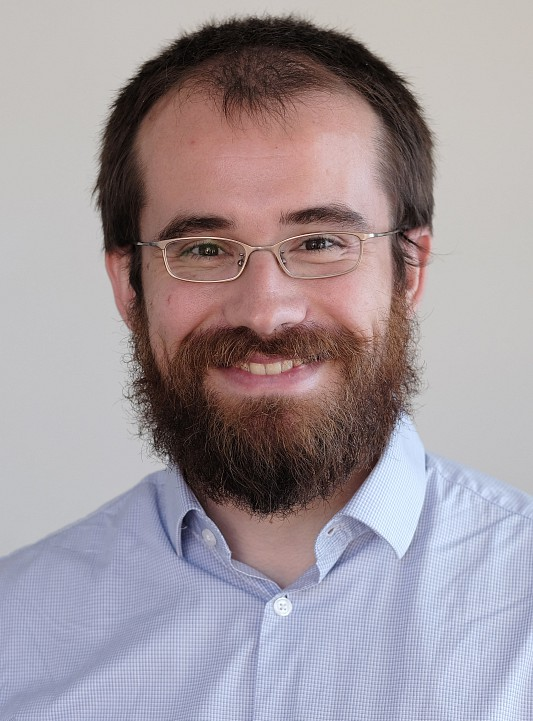
\includegraphics[height=2.5cm]{figures/team_rufus_lawrence.jpg}\hspace{1mm}%
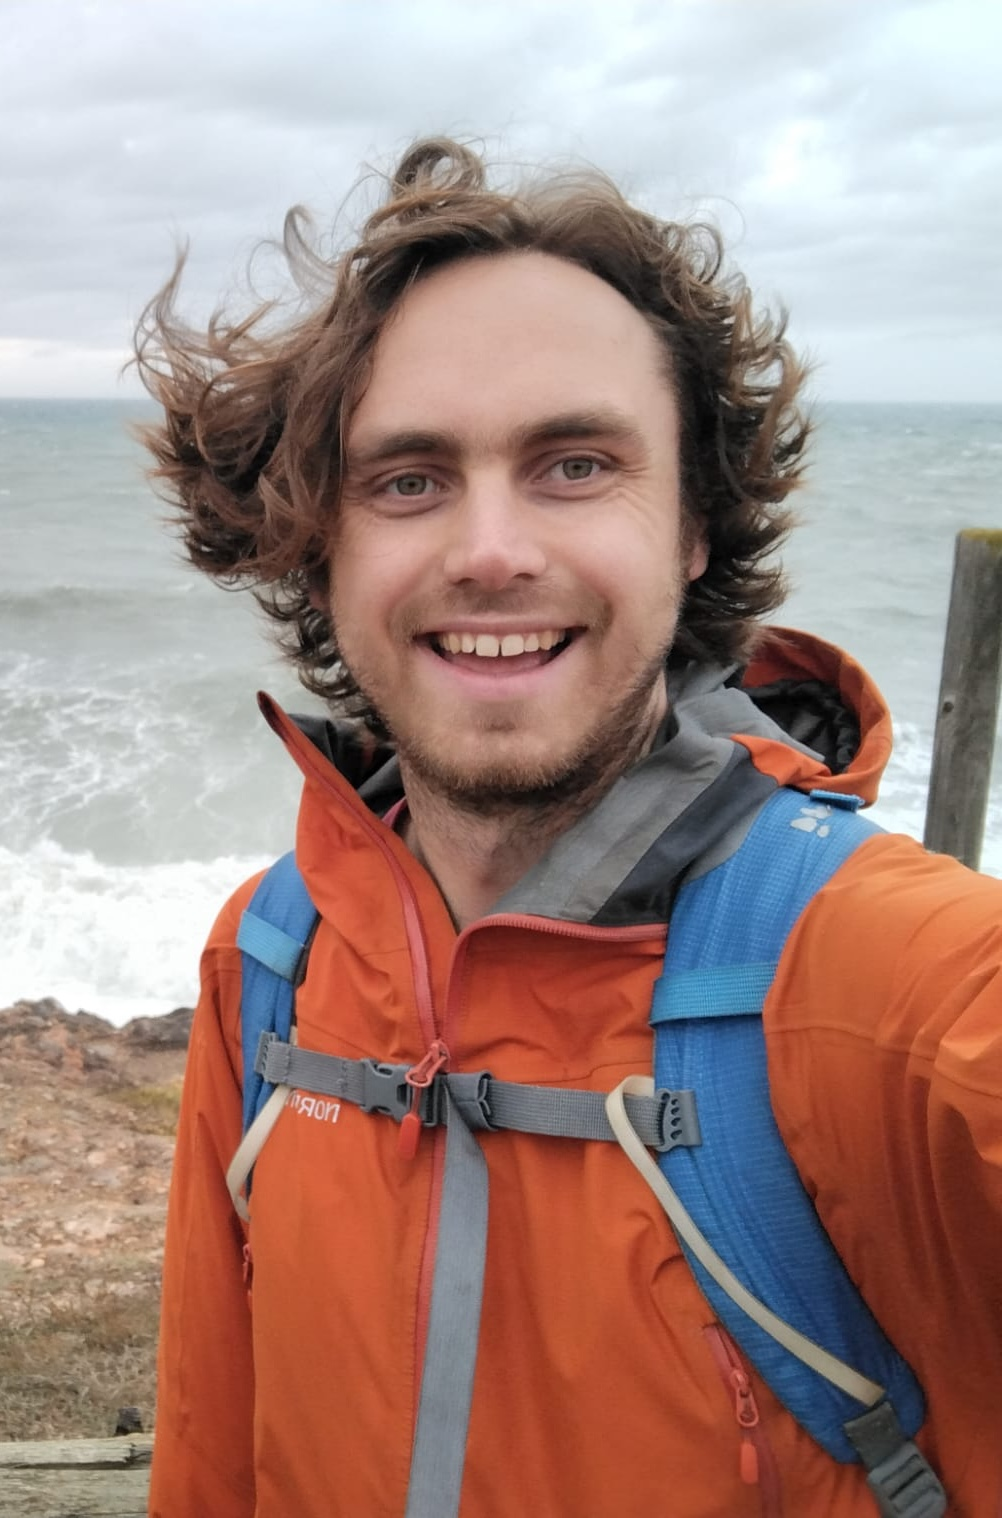
\includegraphics[height=2.5cm]{figures/team_waqas_parvaiz.jpg}}
\end{column}
\end{columns}
\medskip
\textbf{Lectures/Tutorials:} Wednesdays, 11:00--12:30 and 12:45--14:15, room KN:A-311.
\ona{\todo{Confirm the roles of the team members for this year (in particular Lloren{\c c}'s), and that the portraits are attributed correctly; no portrait of Lloren{\c c} yet.}}
\end{frame}

\begin{frame}\ft{Prerequisites}
\ona{We assume linear algebra (including the spectral theorem and tensor products), basic probability, and the rudiments of ordinary differential equations. No prior knowledge of quantum mechanics or of control theory is assumed; \Chap~\ref{C.Closed} summarises what is needed of the former, and the classical control-theoretic notions are introduced alongside their quantum counterparts. Familiarity with conic optimization at the level of today's second half suffices. Three courses are natural companions but not prerequisites: BQM36PMO, \emph{Conic optimization}, from which the second half of this \chap{} is drawn; BE3M35ORR, \emph{Optimal and Robust Control}, whose classical theory (Pontryagin's principle, linear-quadratic and robust design) is the counterpart of \Chaps~\ref{C.GeometryControl} and~\ref{C.AlgControl}; and BQM36QEC, \emph{Quantum Error Correction}, which takes the noise models of \Chap~\ref{C.Open} as its starting point.}
\onp{\begin{itemize}
    \item Prerequisites: linear algebra, probability, ODEs. \emph{No} quantum mechanics or control theory assumed.
    \item Related courses (companions, not prerequisites): \alert{BQM36PMO} \emph{Conic optimization}, \alert{BE3M35ORR} \emph{Optimal and Robust Control}, and \alert{BQM36QEC} \emph{Quantum Error Correction}; today's refresher covers what is needed of the first.
    \item Materials: slides and handouts share one source; figures and code are Python scripts in \texttt{code/}.
    \item Optional (not required) reading: \citet{dalessandro2021introduction}, \citet{borzi2017formulation}, and \citet{nie2023moment} for the polynomial optimization.
\end{itemize}}
\ona{Optional reading material is available in the textbook of \citet{dalessandro2021introduction}, \emph{Introduction to Quantum Control and Dynamics}, in the SIAM book of \citet{borzi2017formulation}, \emph{Formulation and Numerical Solution of Quantum Control Problems}, and, for the polynomial optimization used in the algorithmic \chaps{}, in \citet{nie2023moment}, \emph{Moment and Polynomial Optimization}; none of them is required, and these notes are self-contained.}
\end{frame}

\begin{frame}\ft{Assessment}
In total, you can earn a maximum of 100 points for the course and receive a grade from A to F ($<50$ points $=$ F, 50--59 $=$ E, 60--69 $=$ D, 70--79 $=$ C, 80--89 $=$ B, 90--100 $=$ A).
Points are earned through semester activities (up to 60 points in total) and the exam (up to 40 points).

\textbf{Course credit: semester activity (max.\ 60 points).}
You can earn semester points by completing assignments\ona{ (see the \texttt{exercises/} folder; they build up, step by step, a simulator and an identification and control toolbox for small open quantum systems in Python)}.
For all assignments, the last submitted solution is the one considered for grading.
To receive course credit, you must earn at least 30 out of 60 points and attend the practical classes regularly. One absence is permitted.

\textbf{Exam (max.\ 40 points).}
Theoretical part of the exam (max.\ 40 points)\ona{, covering \Chaps~\ref{C.Closed}--\ref{C.AlgControl}}. If multiple successful attempts are made, the highest score achieved is considered.
\end{frame}

\section{Why quantum optimal control?}

\begin{frame}\ft{Why control quantum systems?}
\ona{Every quantum technology---computers, sensors, clocks, communication links---is, at the level of the hardware, a driven quantum system: a handful of two-level atoms, superconducting circuits, or trapped ions, steered by classical electromagnetic fields that an engineer shapes in time. The promise of the technology rests on our ability to steer these systems precisely, and to know precisely what we are steering. This course is about both halves of that sentence: \emph{identification} (learning the model from measurement data) and \emph{control} (shaping the fields), and about the geometry that ties the two together.}

\ona{We adopt the point of view of a control engineer. A quantum device is a dynamical system with inputs, outputs, and an internal state. The peculiarity is that the state is never observed directly: a measurement returns one sample from a probability distribution determined by the state, and destroys the state in the process. The classical questions of systems theory---controllability, observability, identifiability, sample complexity, optimality---all need to be asked again.}

\onp{\begin{itemize}\setlength\itemsep{1em}
    \item Quantum hardware $=$ a driven dynamical system with classical inputs $u(t)$.
    \item State (density operator $\rho$) is never observed directly; measurements are destructive and statistical.
    \item Two questions: \alert{identification} (what is the system?) and \alert{control} (how do we steer it?).
    \item Bridge between them: the \alert{geometry} of states, channels, and control landscapes.
\end{itemize}}
\end{frame}

\begin{frame}\ft{Outline}
\ona{After the plan of the course, the first half of this \chap{} introduces six examples, each taken from a research paper whose results we will meet later in the course. We keep the mathematics to a minimum; the point is to see what kinds of questions are asked. The second half is a compact refresher of conic optimization---the computational tool behind several of the algorithms of \Chaps~\ref{C.AlgTomography} and~\ref{C.AlgControl}---which doubles as a first exposure for those who have not taken the conic optimization course.}

\onp{Outline of today's lecture:
\begin{itemize}\setlength\itemsep{0.5em}
    \item A short tour of the hardware: what is in a quantum computer, and what the control field is.
    \item Six examples: state tomography; a driven qubit; gate synthesis with traps; a noisy qubit; identifying a two-qubit open system; gates from local interactions.
    \item Conic optimization, a refresher: cones and solvers, duality, sums of squares, the moment-SOS hierarchy.
\end{itemize}}
\ona{\medskip\noindent\textit{Sources.} This \chap{} draws on \citep{ansel2024introduction,bondar2025globally,lawrence2026geometric,parvaiz2025identifiability,lawrence2026penalised,parvaiz2026survey}; passages from these papers are reproduced with light editing, whereas material from the tutorial of \citet{ansel2024introduction} is paraphrased.}
\onp{\vfill{\scriptsize Sources: \citep{ansel2024introduction,bondar2025globally,lawrence2026geometric,parvaiz2025identifiability,lawrence2026penalised,parvaiz2026survey}.}}
\end{frame}

\begin{frame}<presentation>\ft{Agenda}
\qocAgendaBody{2}
\end{frame}

\section{Qubits and how to implement them}

\begin{frame}\ft{Most quantum computers so far look like this}
\ona{Before the abstractions, a look at the hardware whose behaviour the models of \Chaps~\ref{C.Closed}--\ref{C.Open} are meant to capture. A superconducting quantum computer is a dilution cryostat cooled to about 10\,mK, holding a chip with the qubits on a circuit board, connected through very special (and fragile) wiring to room-temperature electronics: signal sources, FPGA-based pulse-shaping units, and digitisers. \emph{The control field $u(t)$ of this course is the pulse produced by those units}; what physical form it takes (microwave, laser, voltage, magnetic field) depends on the architecture, and its imperfections, together with the wiring, are a large part of the noise.}
\onp{\begin{columns}[T]
\begin{column}{0.38\textwidth}
\begin{itemize}\setlength\itemsep{0.3em}
    \item A very expensive cryostat (Bluefors), $\approx 10$\,mK.
    \item Very special wires (easy to break at $<1$\,K).
    \item Qubits on a chip, on a circuit board.
    \item Room-temperature electronics: signal sources, FPGA-based pulse shaping, digitisation.
    \item \alert{$u(t)$ of this course $=$ the shaped pulse}, whatever its physical carrier in a given architecture.
\end{itemize}
\end{column}
\begin{column}{0.60\textwidth}
\centering
\resizebox{!}{0.8\textheight}{% Generated by code/ch01_hardware.py -- do not edit by hand.
\definecolor{qocA}{rgb}{0.00,0.45,0.70}
\definecolor{qocB}{rgb}{0.90,0.60,0.00}
\definecolor{qocC}{rgb}{0.00,0.62,0.45}
\definecolor{qocD}{rgb}{0.80,0.40,0.00}
\definecolor{qocE}{rgb}{0.80,0.60,0.70}
\definecolor{qocF}{rgb}{0.35,0.70,0.90}
\begin{tikzpicture}[x=1cm,y=1cm]

% background: the cryostat
\node[anchor=south west, inner sep=0] (cryo) at (0,0) {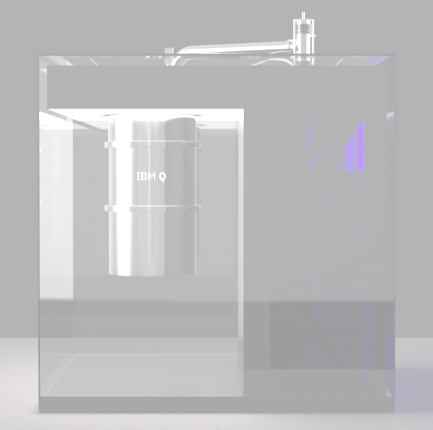
\includegraphics[width=8.00cm]{figures/hw_cryostat.png}};
% wiring stages, seen inside the can (left-centre of the photograph)
\node[anchor=center, inner sep=0, draw=white, line width=0.6pt] (wires) at (2.40,5.04) {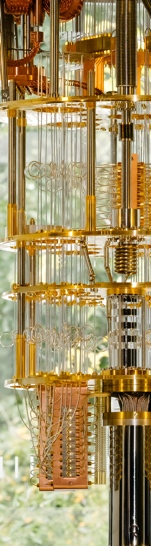
\includegraphics[height=2.72cm]{figures/hw_wires.jpg}};
% zoom 1: the printed circuit board at the bottom of the cryostat
\node[anchor=center, inner sep=0, draw=qocB, line width=1pt] (pcb) at (2.72,2.08) {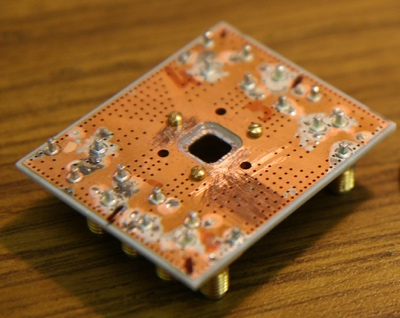
\includegraphics[width=3.20cm]{figures/hw_board.jpg}};
% zoom 2: the qubit chip at the centre of the board
\node[anchor=center, inner sep=0, draw=qocA, line width=1pt] (chip) at (pcb.center) {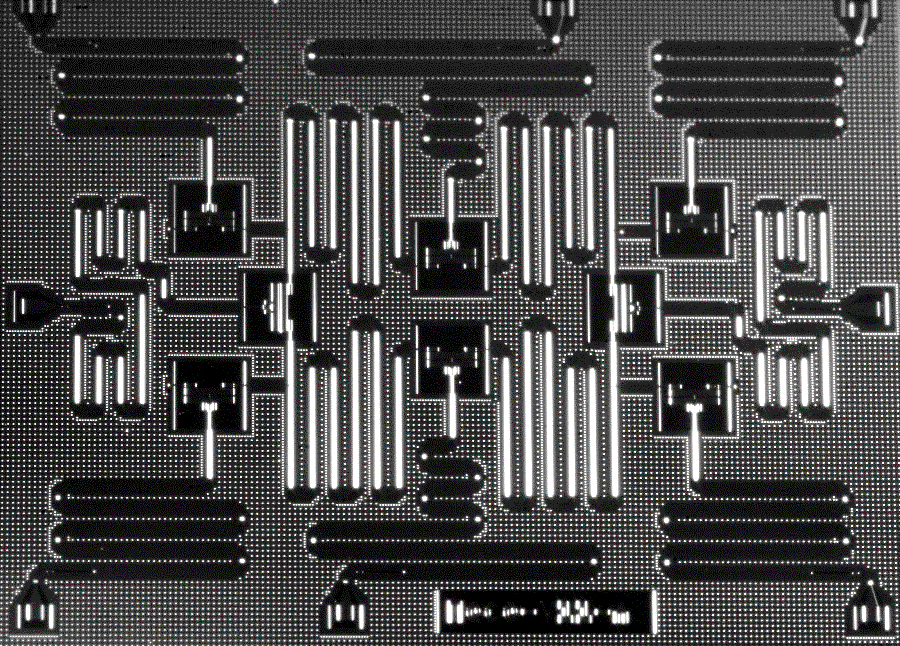
\includegraphics[width=1.36cm]{figures/hw_chip.png}};
% zoom lines
\draw[qocB, thick, dashed] (wires.south west) -- (pcb.north west);
\draw[qocB, thick, dashed] (wires.south east) -- (pcb.north east);
\draw[qocA, thick, dashed] ($(pcb.center)+(-0.12,-0.10)$) -- (chip.south west);
\draw[qocA, thick, dashed] ($(pcb.center)+(0.12,-0.10)$) -- (chip.south east);
% room-temperature electronics, placed over the right half of the cabinet
\node[anchor=south, inner sep=0, draw=white, line width=0.6pt] (rack) at (6.08,2.40) {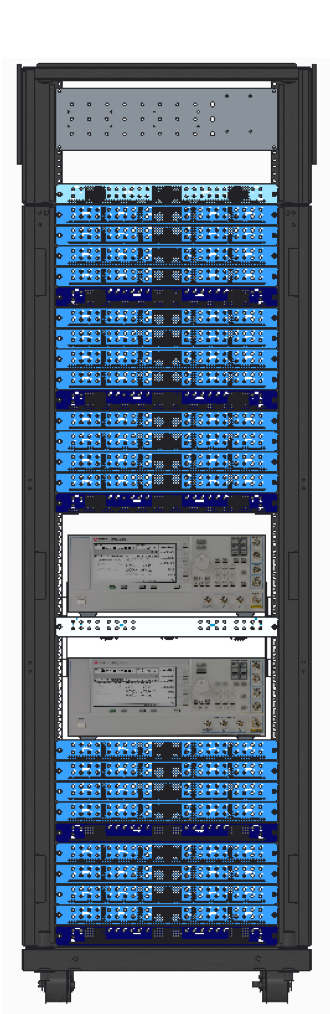
\includegraphics[height=4.80cm]{figures/hw_electronics.png}};
% labels
\small
\node[anchor=north west, align=left, font=\small\bfseries, fill=white, fill opacity=0.8, text opacity=1, inner sep=1.5pt] at (0.05,7.95) {dilution cryostat (Bluefors),\\ about 10\,mK};
\node[anchor=west, align=left, fill=white, fill opacity=0.8, text opacity=1, inner sep=1pt, font=\footnotesize] at ($(wires.east)+(0.06,0.5)$) {wiring and\\ filtering stages\\ (fragile below 1\,K)};
\node[anchor=north, align=center, fill=white, fill opacity=0.8, text opacity=1, inner sep=1pt, text=qocB] at ($(pcb.south)+(0,-0.05)$) {circuit board (zoom)};
\node[anchor=south, align=center, fill=white, fill opacity=0.8, text opacity=1, inner sep=1pt, text=qocA] at ($(chip.north)+(0,0.03)$) {qubit chip (zoom)};
\node[anchor=north, align=center, font=\small, text width=2.88cm, fill=white, fill opacity=0.85, text opacity=1, inner sep=2pt] at ($(rack.south)+(0,-0.08)$) {room-temperature electronics: signal sources, FPGA pulse shaping, digitisers -- \alert{this is where $u(t)$ is made}};
\node[anchor=north east, font=\tiny, fill=white, fill opacity=0.8, text opacity=1, inner sep=1pt] at (8.00-0.05,7.95) {Image credit: IBM.};
\end{tikzpicture}
}
\end{column}
\end{columns}}
\ona{\begin{figure}[h]\centering\resizebox{0.62\linewidth}{!}{% Generated by code/ch01_hardware.py -- do not edit by hand.
\definecolor{qocA}{rgb}{0.00,0.45,0.70}
\definecolor{qocB}{rgb}{0.90,0.60,0.00}
\definecolor{qocC}{rgb}{0.00,0.62,0.45}
\definecolor{qocD}{rgb}{0.80,0.40,0.00}
\definecolor{qocE}{rgb}{0.80,0.60,0.70}
\definecolor{qocF}{rgb}{0.35,0.70,0.90}
\begin{tikzpicture}[x=1cm,y=1cm]

% background: the cryostat
\node[anchor=south west, inner sep=0] (cryo) at (0,0) {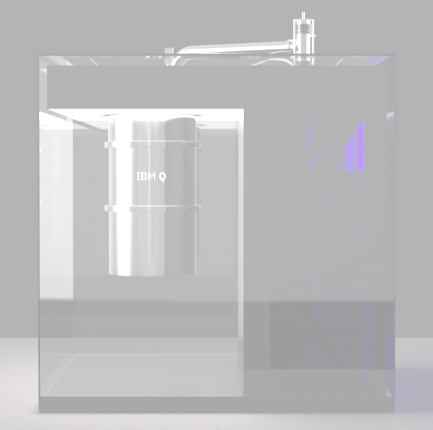
\includegraphics[width=8.00cm]{figures/hw_cryostat.png}};
% wiring stages, seen inside the can (left-centre of the photograph)
\node[anchor=center, inner sep=0, draw=white, line width=0.6pt] (wires) at (2.40,5.04) {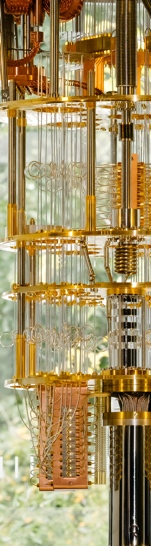
\includegraphics[height=2.72cm]{figures/hw_wires.jpg}};
% zoom 1: the printed circuit board at the bottom of the cryostat
\node[anchor=center, inner sep=0, draw=qocB, line width=1pt] (pcb) at (2.72,2.08) {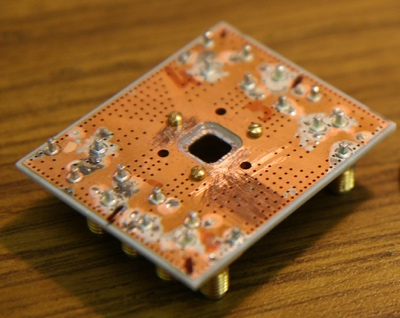
\includegraphics[width=3.20cm]{figures/hw_board.jpg}};
% zoom 2: the qubit chip at the centre of the board
\node[anchor=center, inner sep=0, draw=qocA, line width=1pt] (chip) at (pcb.center) {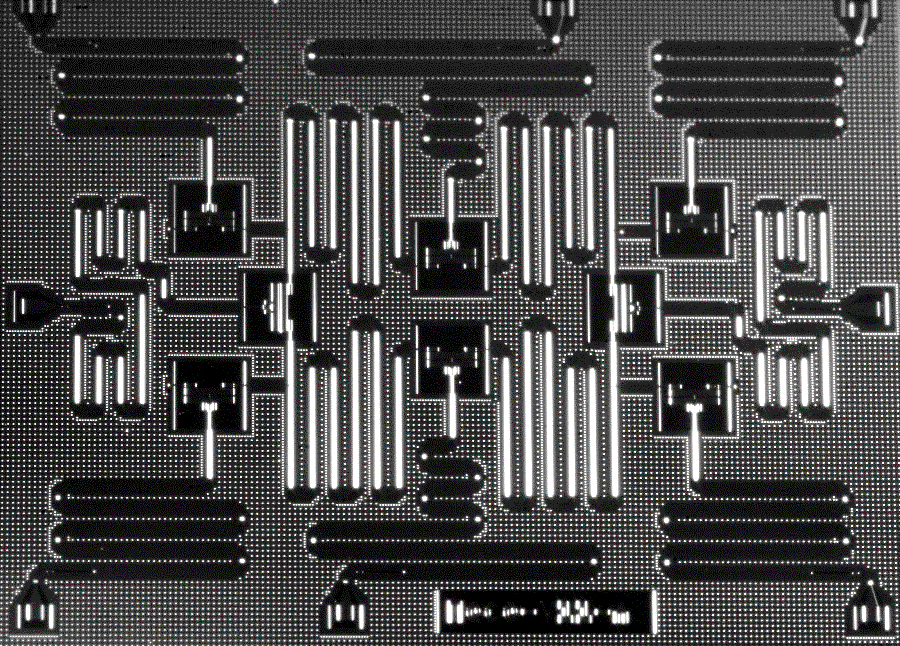
\includegraphics[width=1.36cm]{figures/hw_chip.png}};
% zoom lines
\draw[qocB, thick, dashed] (wires.south west) -- (pcb.north west);
\draw[qocB, thick, dashed] (wires.south east) -- (pcb.north east);
\draw[qocA, thick, dashed] ($(pcb.center)+(-0.12,-0.10)$) -- (chip.south west);
\draw[qocA, thick, dashed] ($(pcb.center)+(0.12,-0.10)$) -- (chip.south east);
% room-temperature electronics, placed over the right half of the cabinet
\node[anchor=south, inner sep=0, draw=white, line width=0.6pt] (rack) at (6.08,2.40) {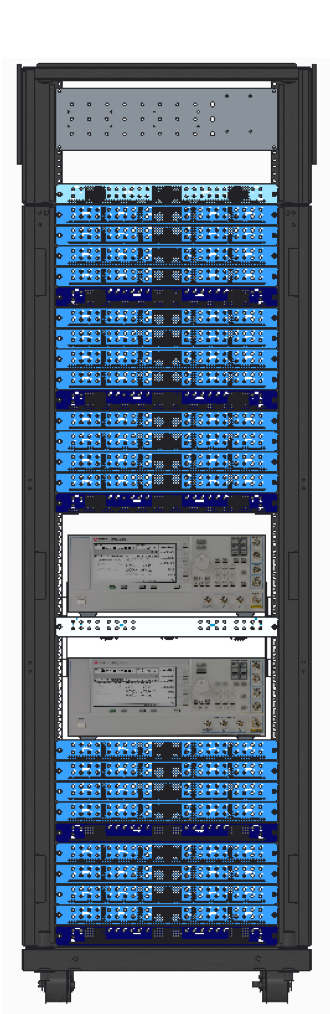
\includegraphics[height=4.80cm]{figures/hw_electronics.png}};
% labels
\small
\node[anchor=north west, align=left, font=\small\bfseries, fill=white, fill opacity=0.8, text opacity=1, inner sep=1.5pt] at (0.05,7.95) {dilution cryostat (Bluefors),\\ about 10\,mK};
\node[anchor=west, align=left, fill=white, fill opacity=0.8, text opacity=1, inner sep=1pt, font=\footnotesize] at ($(wires.east)+(0.06,0.5)$) {wiring and\\ filtering stages\\ (fragile below 1\,K)};
\node[anchor=north, align=center, fill=white, fill opacity=0.8, text opacity=1, inner sep=1pt, text=qocB] at ($(pcb.south)+(0,-0.05)$) {circuit board (zoom)};
\node[anchor=south, align=center, fill=white, fill opacity=0.8, text opacity=1, inner sep=1pt, text=qocA] at ($(chip.north)+(0,0.03)$) {qubit chip (zoom)};
\node[anchor=north, align=center, font=\small, text width=2.88cm, fill=white, fill opacity=0.85, text opacity=1, inner sep=2pt] at ($(rack.south)+(0,-0.08)$) {room-temperature electronics: signal sources, FPGA pulse shaping, digitisers -- \alert{this is where $u(t)$ is made}};
\node[anchor=north east, font=\tiny, fill=white, fill opacity=0.8, text opacity=1, inner sep=1pt] at (8.00-0.05,7.95) {Image credit: IBM.};
\end{tikzpicture}
}\caption{A superconducting quantum computer, from the outside in: the dilution cryostat, the wiring and filtering stages inside the can, the printed circuit board at its bottom (zoom), and the qubit chip at the centre of the board (zoom); to the right, the room-temperature electronics that generate the control pulses. Photographs: IBM; composition by \texttt{code/ch01\_hardware.py}.}\label{fig:ch01:hardware}\end{figure}}
\end{frame}

\begin{frame}\ft{``What is on the chip'' differs}
\onp{\begin{columns}[T]
\begin{column}{0.45\textwidth}
\begin{itemize}\setlength\itemsep{0.4em}
    \item Superconducting qubits (transmon, \ldots)
    \item Double quantum dots (in Si, Ge, \ldots)
    \item Photonic qubits
    \item Ions and neutral atoms
    \item Fullerenes, carbon nanotubes, etc.
\end{itemize}
\end{column}
\begin{column}{0.53\textwidth}
\centering
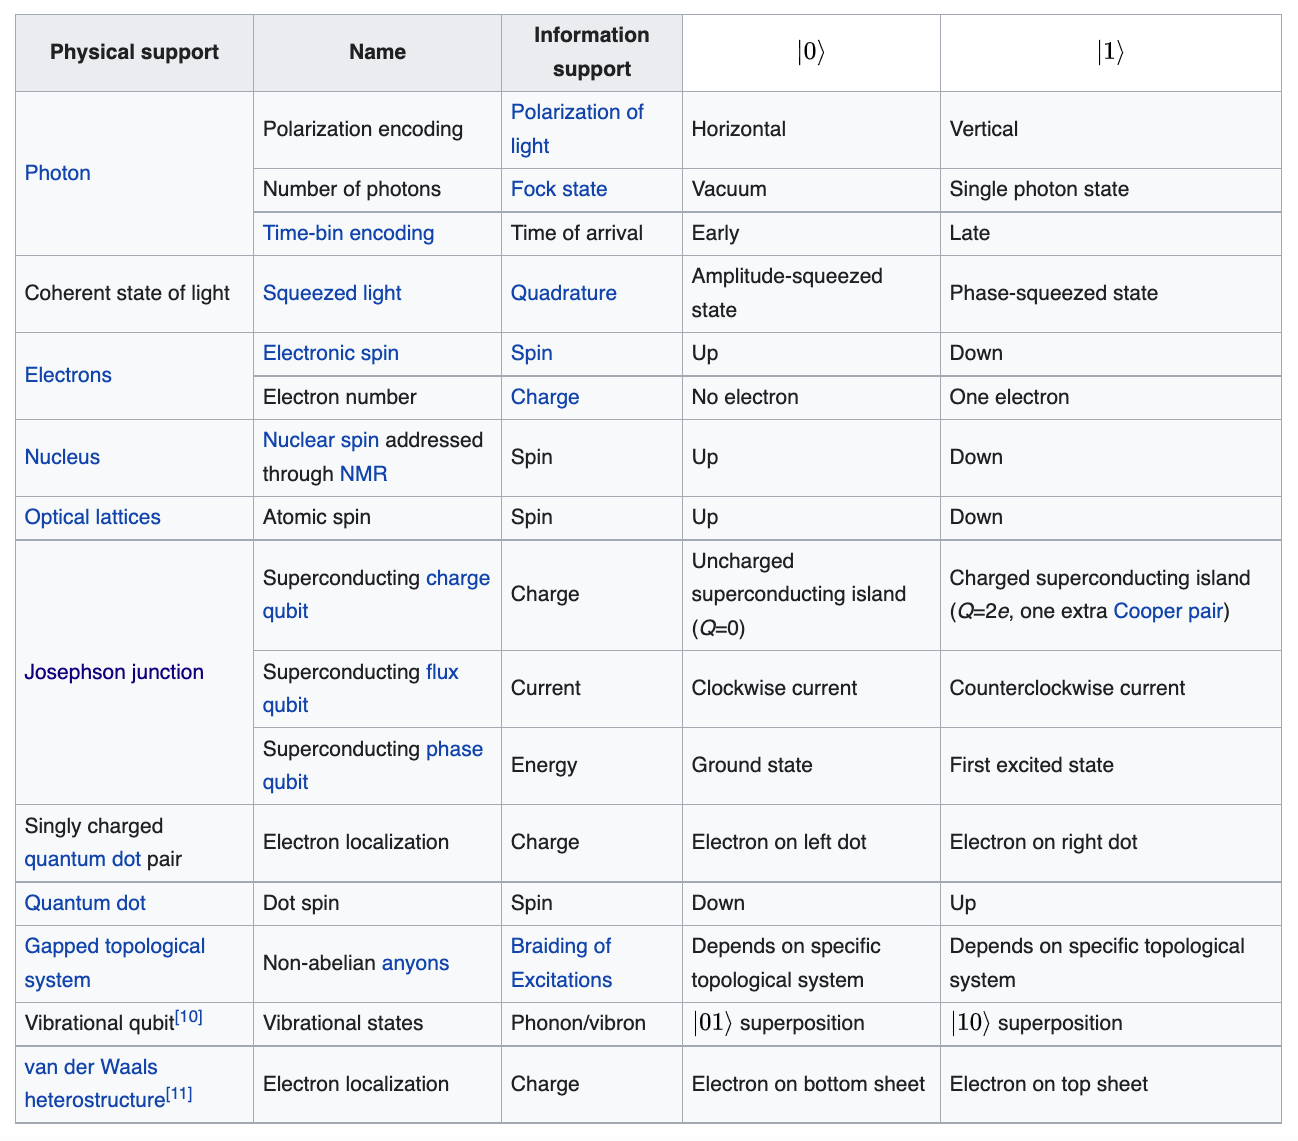
\includegraphics[width=\linewidth]{figures/hw_qubit_table_wikipedia.png}\\
{\tiny \url{https://en.wikipedia.org/wiki/Qubit}}
\end{column}
\end{columns}}
\ona{What sits on the chip differs from one architecture to the next:
\begin{itemize}\setlength\itemsep{0.4em}
    \item Superconducting qubits (transmon, \ldots)
    \item Double quantum dots (in Si, Ge, \ldots)
    \item Photonic qubits
    \item Ions and neutral atoms
    \item Fullerenes, carbon nanotubes, etc.
\end{itemize}
Each platform realises the same abstract object, a two-level system with a controllable Hamiltonian and its own decoherence channels, with vastly different time scales: gate times from nanoseconds (superconducting) to microseconds (atoms), and coherence times from microseconds to seconds. The models we build are platform-agnostic; the numbers plugged into them are not.
\begin{figure}[h]\centering
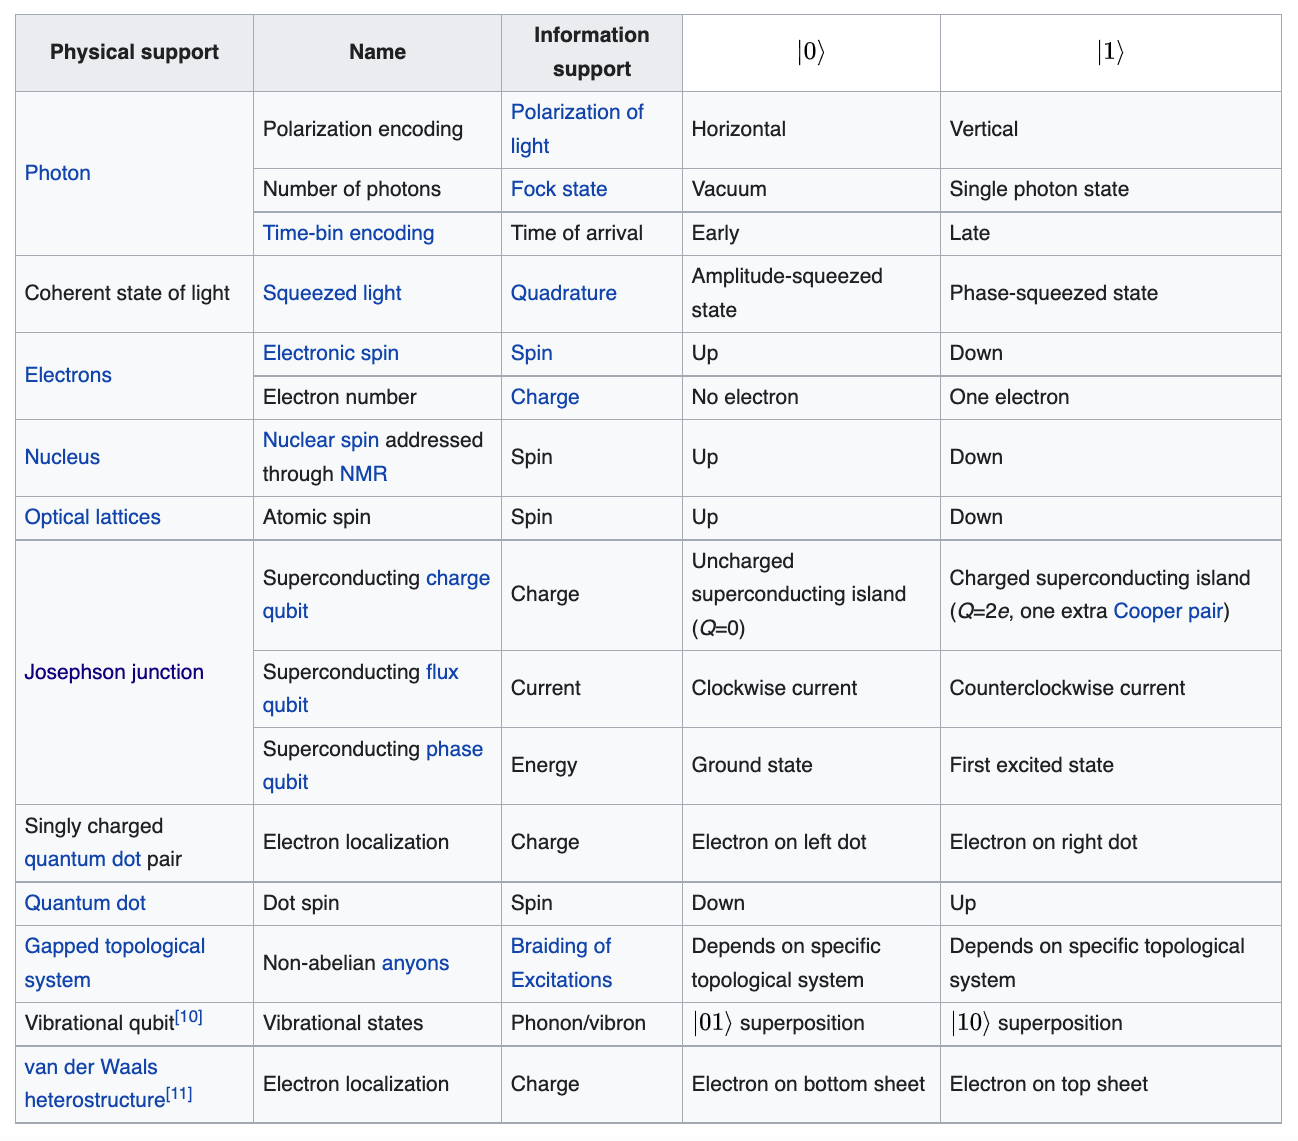
\includegraphics[width=0.75\linewidth]{figures/hw_qubit_table_wikipedia.png}
\caption{Physical realisations of qubits and their characteristic time scales. Source: \url{https://en.wikipedia.org/wiki/Qubit}.}\label{fig:ch01:qubit_table}
\end{figure}}
\end{frame}

\begin{frame}\ft{``What is on the chip'' differs: the industry view}
\onp{\begin{center}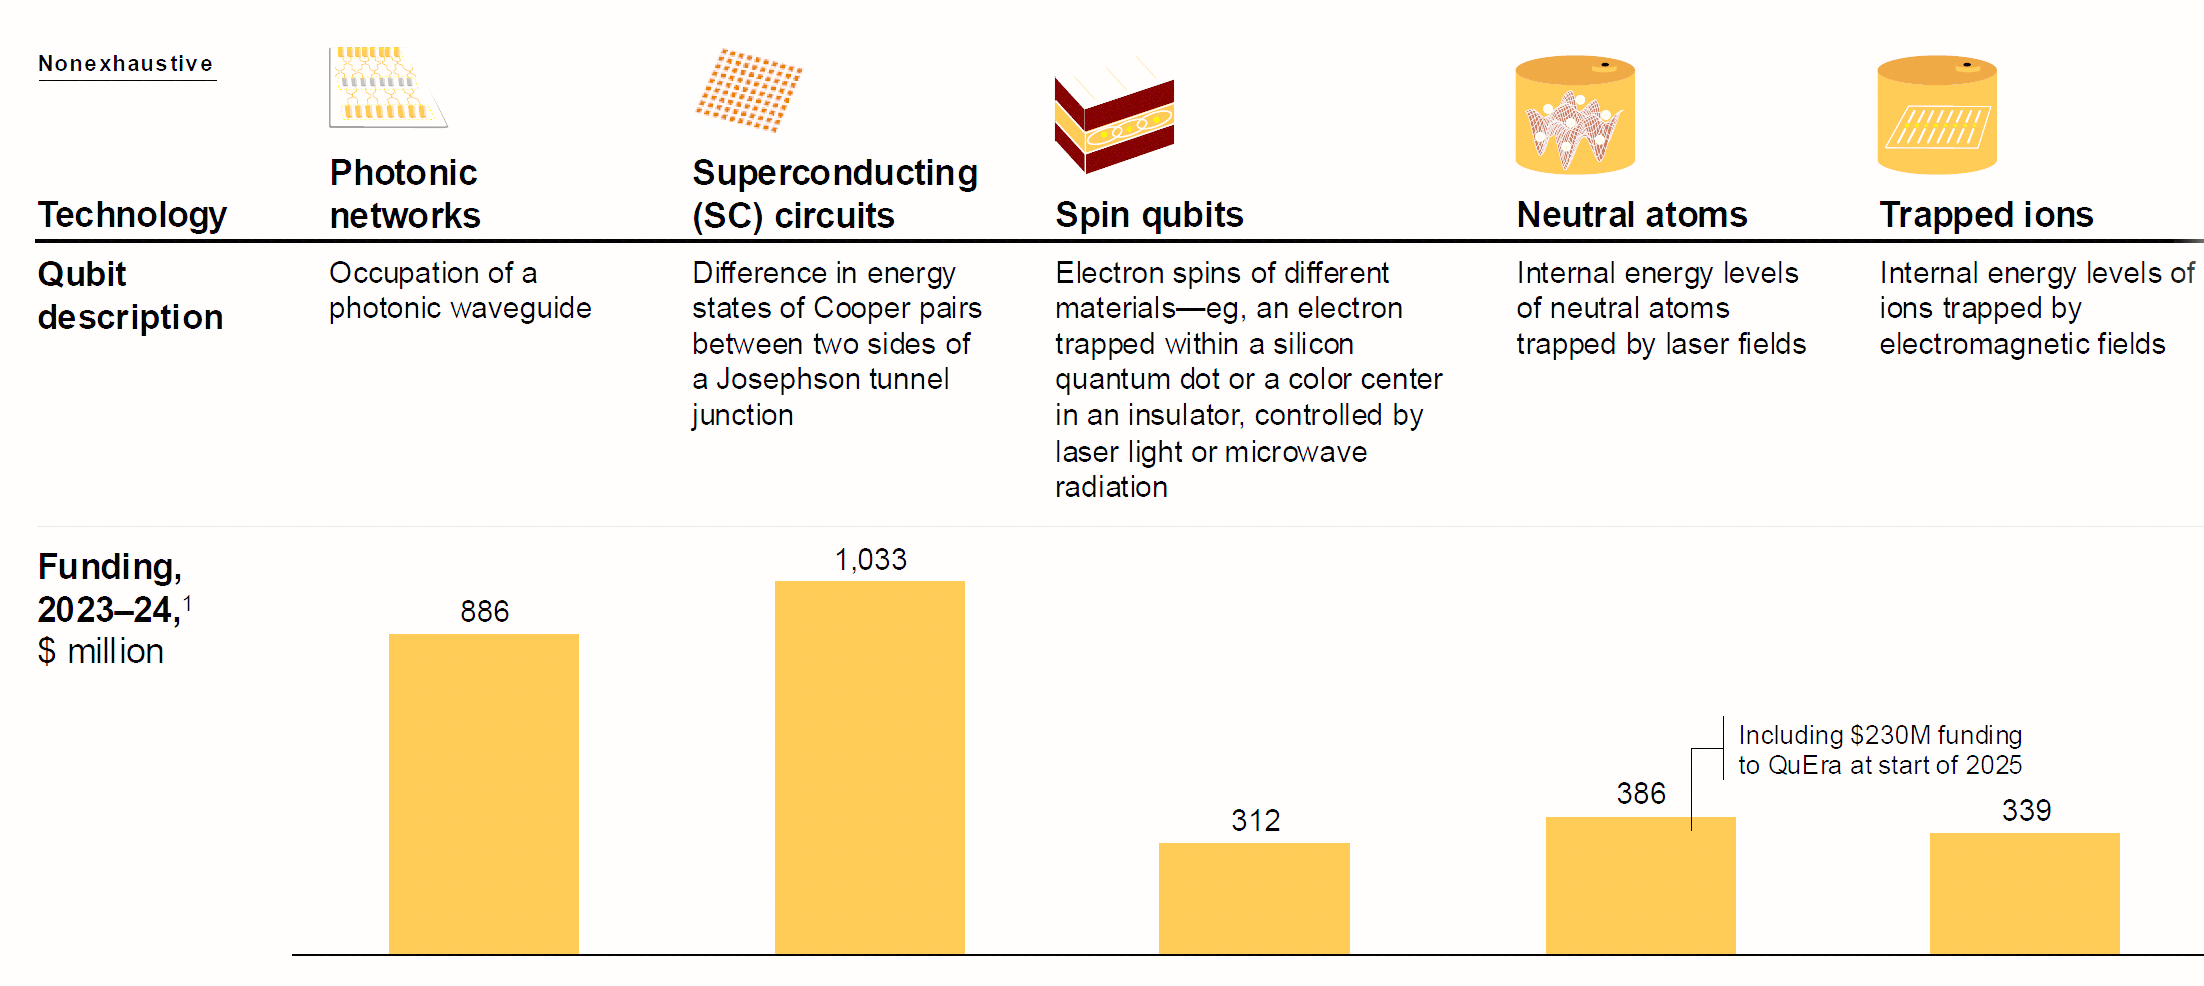
\includegraphics[width=0.95\linewidth]{figures/hw_mckinsey_2025.png}\\
{\tiny \url{https://www.mckinsey.com/capabilities/tech-and-ai/our-insights/the-year-of-quantum-from-concept-to-reality-in-2025}}\end{center}}
\ona{Figure~\ref{fig:ch01:mckinsey} summarises where the main industrial players place their bets across these platforms.
\begin{figure}[h]\centering
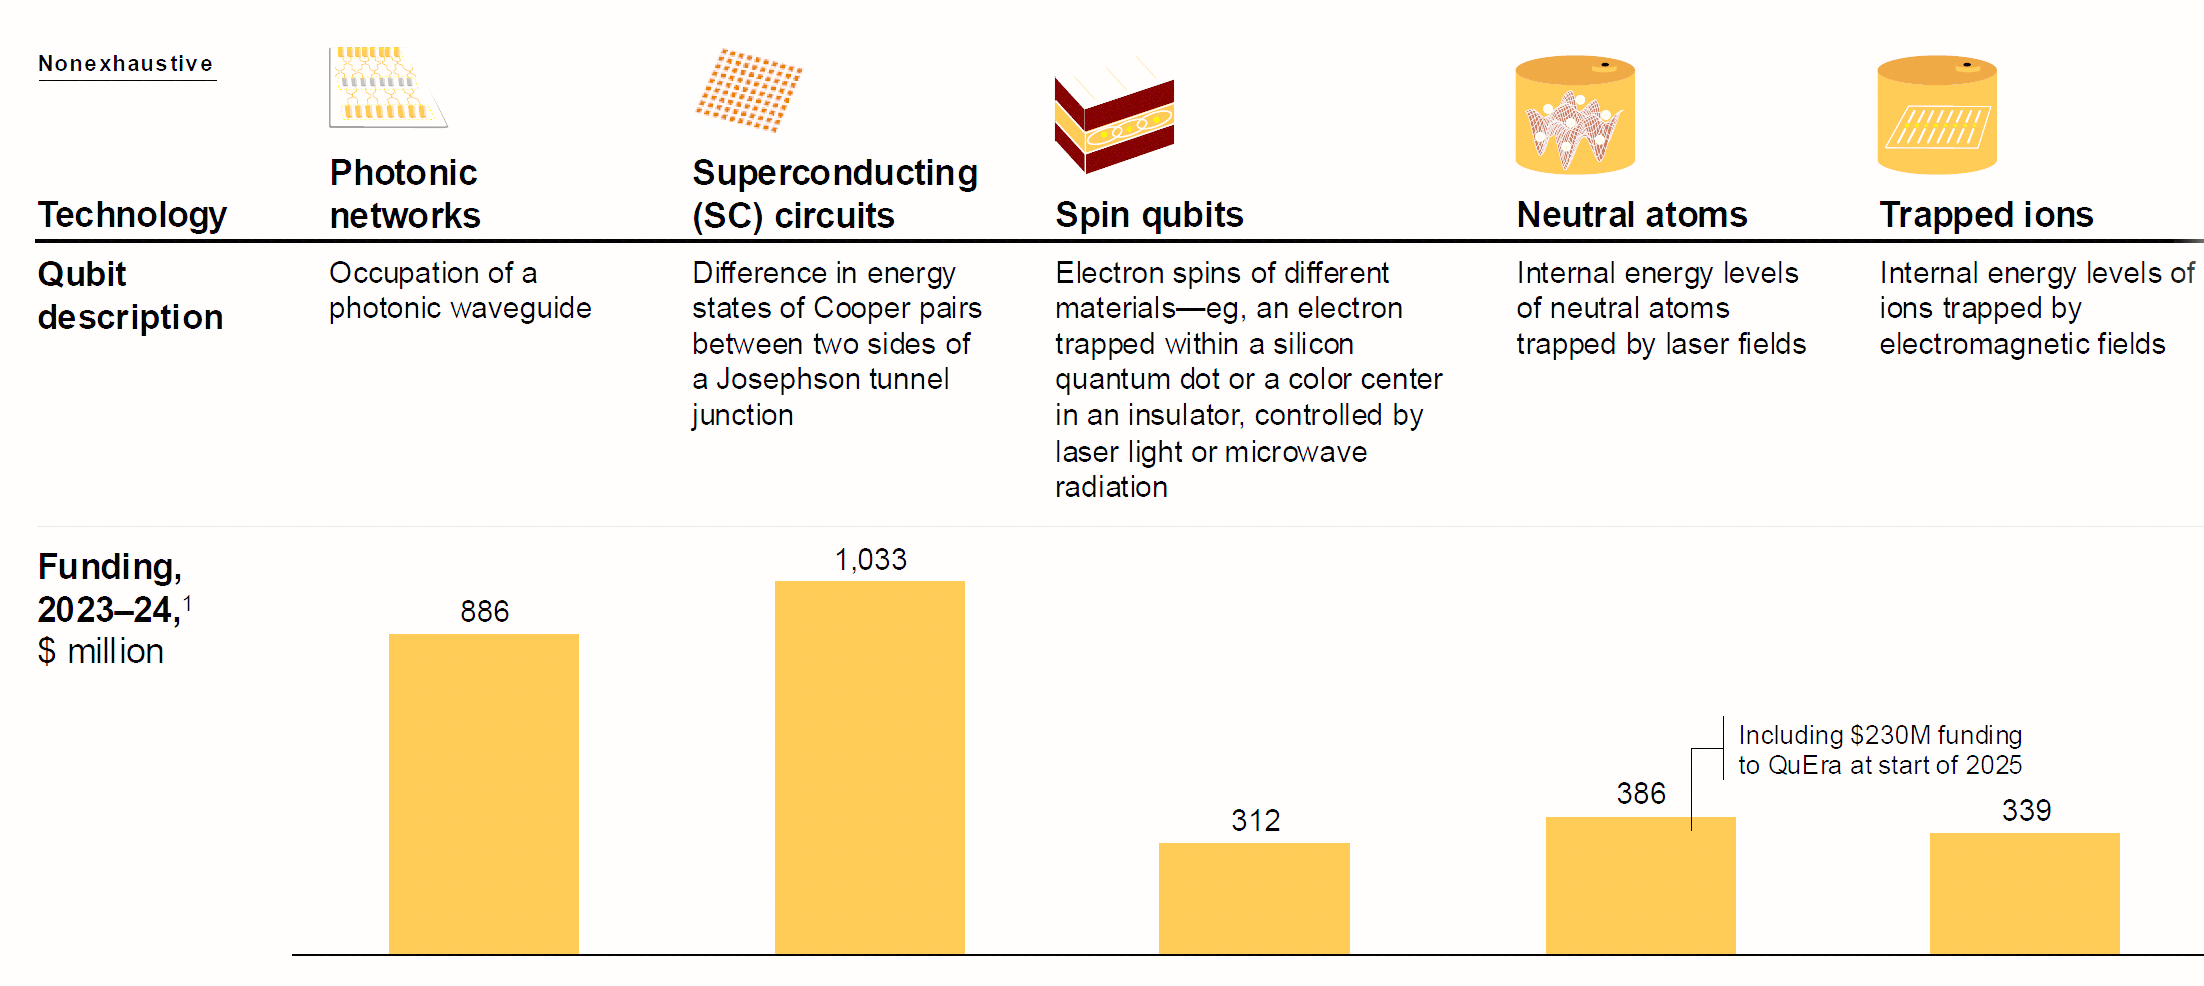
\includegraphics[width=0.8\linewidth]{figures/hw_mckinsey_2025.png}
\caption{The industry view of the qubit platforms. Source: McKinsey, \emph{The year of quantum: from concept to reality in 2025}, \url{https://www.mckinsey.com/capabilities/tech-and-ai/our-insights/the-year-of-quantum-from-concept-to-reality-in-2025}.}\label{fig:ch01:mckinsey}
\end{figure}}
\end{frame}

\begin{frame}\ft{Superconducting qubits}
\onp{\begin{columns}[T]
\begin{column}{0.5\textwidth}
\begin{itemize}\setlength\itemsep{0.4em}
    \item 1962: Josephson effect, tunnelling of superconducting Cooper pairs (Nobel Prize in Physics, 1973).
    \item 1990s: superconducting qubits (Nobel Prize in Physics, 2025).
    \item Based on the Josephson junction, superconducting qubits essentially implement a (weakly anharmonic) quantum oscillator.
    \item Transmon qubits at IBM, Xmon at Google; operated at about 10\,mK.
\end{itemize}
\end{column}
\begin{column}{0.48\textwidth}
\centering
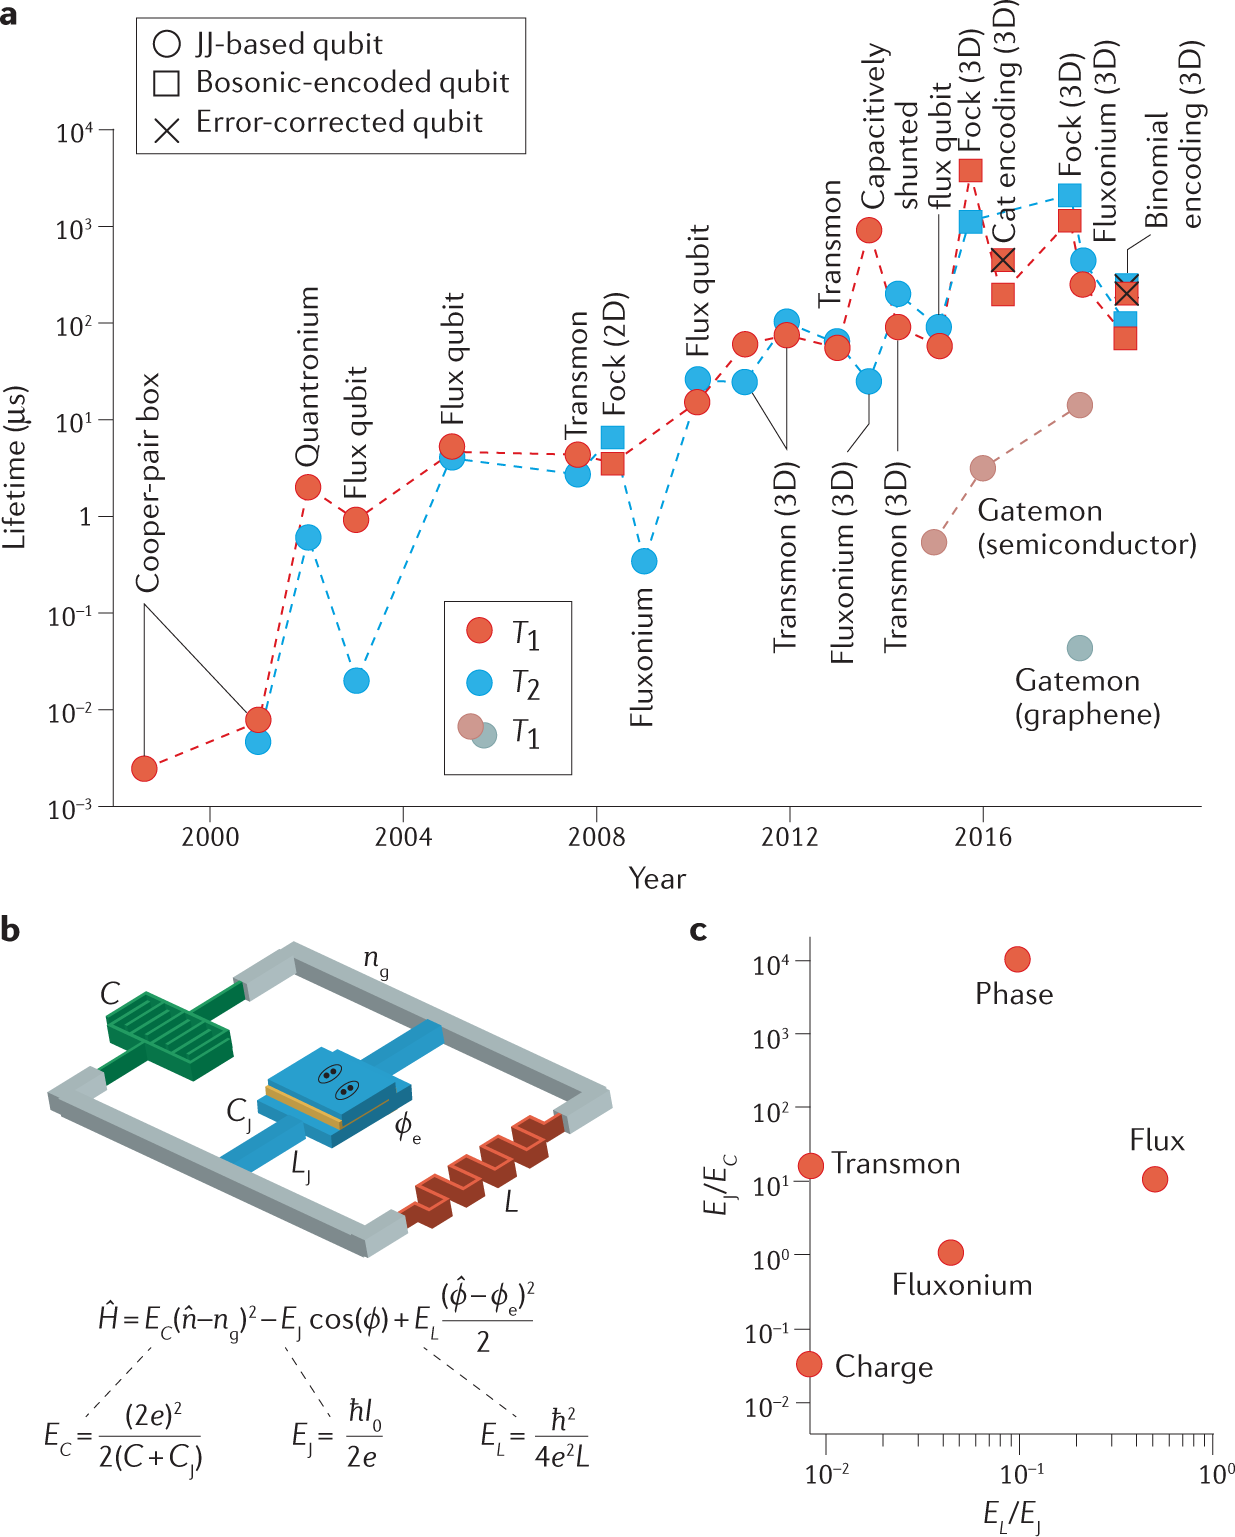
\includegraphics[height=0.62\textheight]{figures/hw_superconducting_nature.png}\\
{\tiny \url{https://www.nature.com/articles/s41578-021-00370-4}}
\end{column}
\end{columns}}
\ona{\begin{itemize}\setlength\itemsep{0.4em}
    \item 1962: Josephson effect, tunnelling of superconducting Cooper pairs (Nobel Prize in Physics, 1973).
    \item 1990s: superconducting qubits (Nobel Prize in Physics, 2025).
    \item Based on the Josephson junction, superconducting qubits essentially implement a (weakly anharmonic) quantum oscillator.
    \item Transmon qubits at IBM, Xmon at Google; operated at about 10\,mK.
\end{itemize}
The anharmonicity is what makes the two lowest levels addressable as a qubit; leakage to the third level is one of the control errors that optimal pulse shaping (\Chap~\ref{C.AlgControl}) is designed to suppress, and the three-level model of Example~C is exactly this system.
\begin{figure}[h]\centering
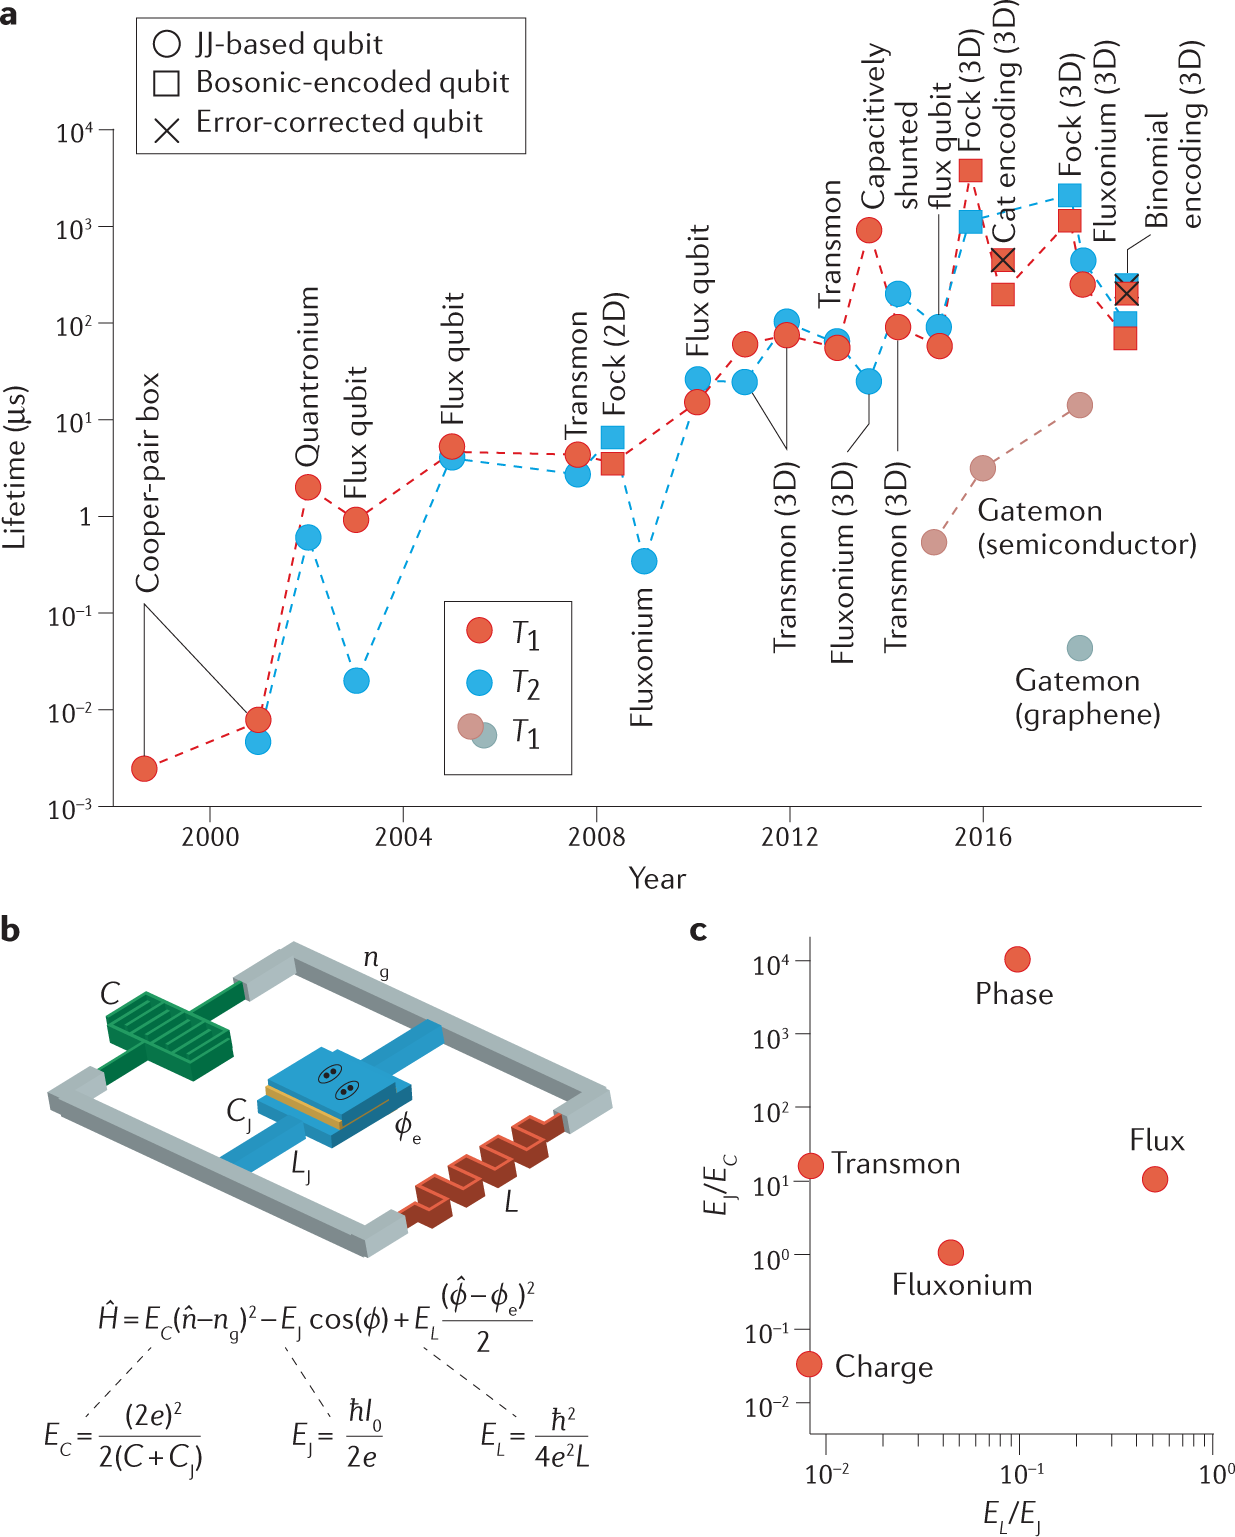
\includegraphics[height=7cm]{figures/hw_superconducting_nature.png}
\caption{Superconducting qubits: from the Josephson junction to the transmon. Source: \url{https://www.nature.com/articles/s41578-021-00370-4}.}\label{fig:ch01:superconducting}
\end{figure}}
\end{frame}

\begin{frame}\ft{Spin qubits in quantum dots}
\onp{\begin{columns}[T]
\begin{column}{0.5\textwidth}
\begin{itemize}\setlength\itemsep{0.3em}
    \item 1963: quantum well with discrete energy values (Kroemer, Alferov, Kazarinov).
    \item Double quantum dots at Intel and elsewhere; operated at about 1\,K, up to 20\,K (Myronov).
\end{itemize}
{\scriptsize
\begin{tabular}{@{}lcc@{}}
 & holes in Ge & electrons in Si\\\hline
effective mass ($m_0$) & 0.035 & 0.19\\
$T_2^*$ & 150\,$\mu$s & 120\,$\mu$s$^{\dagger}$\\
Rabi frequency & 140\,MHz & 10\,MHz\\
1-qubit fidelity & 99.3\,\% & 99.9\,\%\\
\end{tabular}\\ {\tiny $^\dagger$ the community accepts 20\,$\mu$s}}
\end{column}
\begin{column}{0.48\textwidth}
\centering
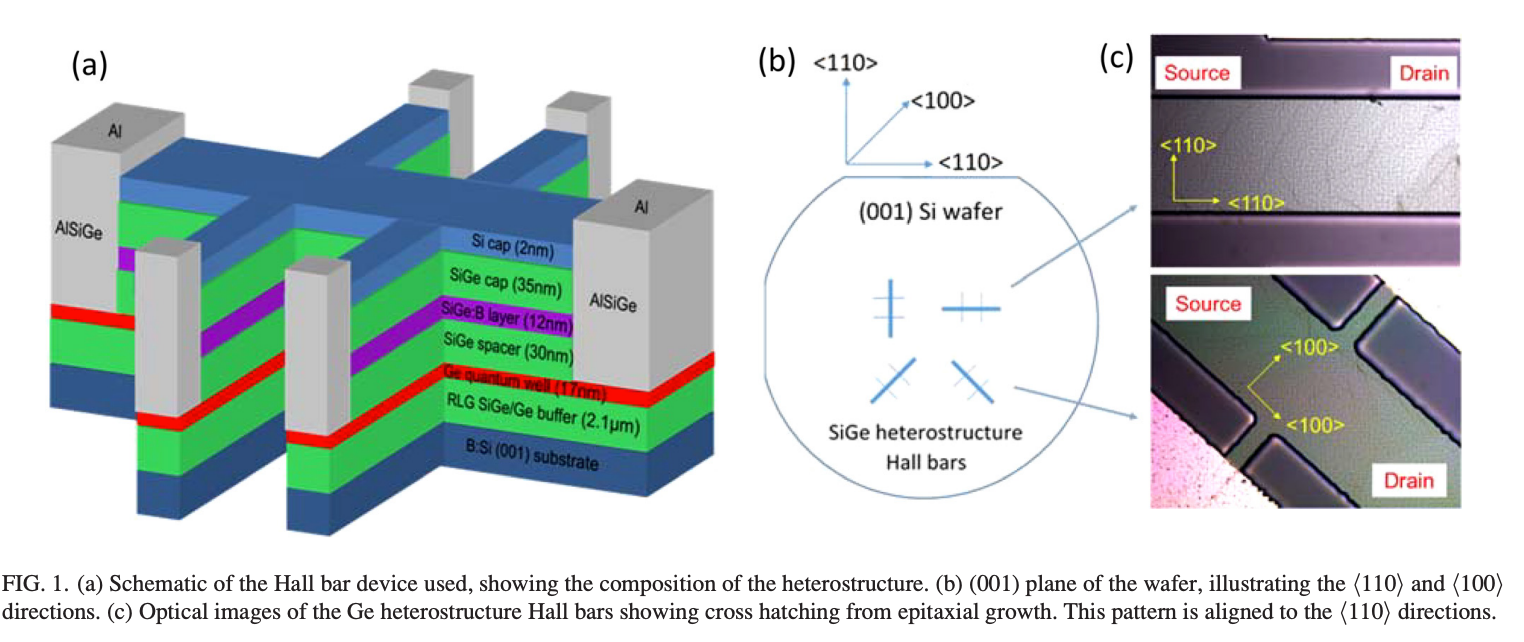
\includegraphics[width=\linewidth]{figures/hw_quantum_dots.png}\\
{\tiny \url{https://aip.scitation.org/doi/full/10.1063/1.5010933}}
\end{column}
\end{columns}}
\ona{\begin{itemize}\setlength\itemsep{0.3em}
    \item 1963: quantum well with discrete energy values (Kroemer, Alferov, Kazarinov).
    \item Double quantum dots at Intel and elsewhere; operated at about 1\,K, up to 20\,K (Myronov).
\end{itemize}
The table is a first encounter with the quantities that identification (\Chaps~\ref{C.StateSpace}--\ref{C.SampleComplexity}) estimates and control (\Chaps~\ref{C.GeometryControl}--\ref{C.AlgControl}) fights against: the Rabi frequency sets how fast $u(t)$ can rotate the state, $T_2^*$ sets how long it has.
\begin{table}[h]\centering\footnotesize
\begin{tabular}{@{}lcc@{}}
 & holes in Ge & electrons in Si\\\hline
effective mass ($m_0$) & 0.035 & 0.19\\
$T_2^*$ & 150\,$\mu$s & 120\,$\mu$s$^{\dagger}$\\
Rabi frequency & 140\,MHz & 10\,MHz\\
1-qubit fidelity & 99.3\,\% & 99.9\,\%\\
\end{tabular}
\caption{Spin qubits in quantum dots: holes in strained germanium versus electrons in silicon. $^\dagger$The community accepts $20\,\mu$s. Source: \url{https://aip.scitation.org/doi/full/10.1063/1.5010933}.}\label{tab:ch01:quantum_dots}
\end{table}
\begin{figure}[h]\centering
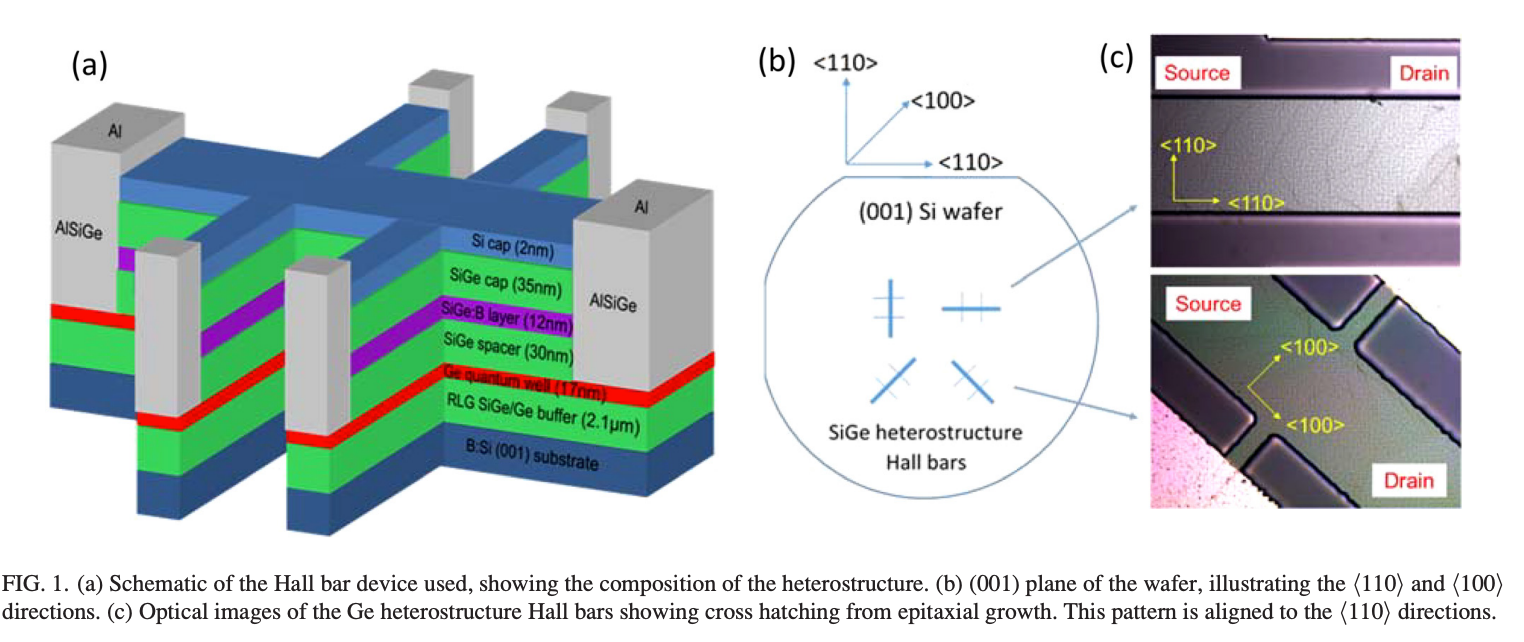
\includegraphics[width=0.8\linewidth]{figures/hw_quantum_dots.png}
\caption{Double quantum dots. Source: \url{https://aip.scitation.org/doi/full/10.1063/1.5010933}.}\label{fig:ch01:quantum_dots}
\end{figure}}
\end{frame}

\begin{frame}\ft{Neutral atoms and ions}
\onp{\begin{columns}[T]
\begin{column}{0.45\textwidth}
\begin{itemize}\setlength\itemsep{0.4em}
    \item Neutral atoms at QuEra, Amazon, Harvard, \ldots: a 2D optical-tweezer array at about 25\,$\mu$K; entangled atoms about 110\,$\mu$m apart.
    \item Ions at IonQ, Alpine Quantum Technologies, Innsbruck, \ldots
\end{itemize}
\end{column}
\begin{column}{0.53\textwidth}
\centering
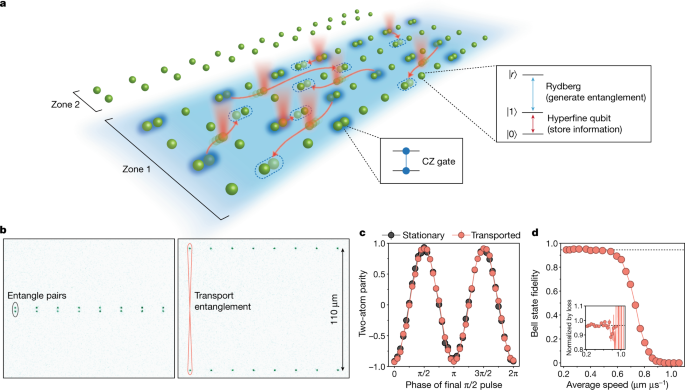
\includegraphics[width=\linewidth]{figures/hw_neutral_atoms.png}\\
{\tiny \url{https://www.nature.com/articles/s41586-022-04592-6}}
\end{column}
\end{columns}}
\ona{\begin{itemize}\setlength\itemsep{0.4em}
    \item Neutral atoms at QuEra, Amazon, Harvard, \ldots: a 2D optical-tweezer array at about 25\,$\mu$K; entangled atoms about 110\,$\mu$m apart.
    \item Ions at IonQ, Alpine Quantum Technologies, Innsbruck, \ldots
\end{itemize}
Here the control fields are laser pulses, the drift Hamiltonian is set by the trap and the atomic structure, and gates are slow but coherence times are long. The same bilinear model of \Chap~\ref{C.Closed} applies, with different numbers.
\begin{figure}[h]\centering
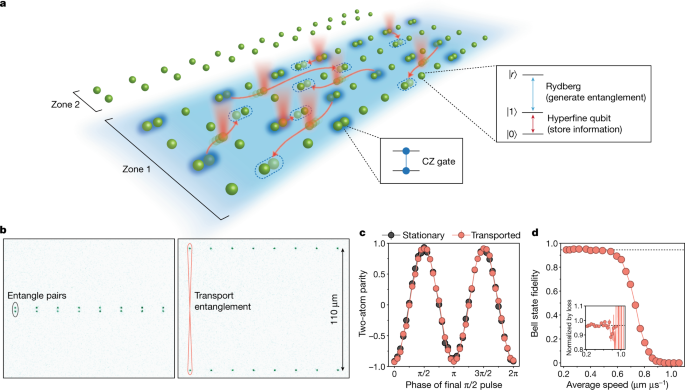
\includegraphics[width=0.8\linewidth]{figures/hw_neutral_atoms.png}
\caption{A two-dimensional array of neutral atoms in optical tweezers. Source: \url{https://www.nature.com/articles/s41586-022-04592-6}.}\label{fig:ch01:neutral_atoms}
\end{figure}}
\end{frame}

\section{Quantum systems as controlled dynamical systems}

\begin{frame}\ft{The minimum in theory}
\mop{\small}
\ona{A finite-level quantum system lives in a Hilbert space $\Hil=\C^d$. Its pure state is a unit vector $\ket{\psi}$, and both the state and the operator $U(T)$ that evolves the system to time $T$ obey the Schr\"odinger equation \cite{NielsenChuang}:}
\onp{Hilbert space $\Hil=\C^d$, state $\ket\psi$ (unit vector), propagator $U(t)$ (unitary):}
\begin{equation}\label{eq:ch01:schrodinger}
    \dd{t}\ket{\psi(t)} = A(t)\ket{\psi(t)},\qquad \dd{t}U(t) = A(t)\,U(t),\quad U(0)=\Id,\qquad A(t)=-\imath H(t).
\end{equation}
\ona{Here $H(t)$ is the Hamiltonian, a Hermitian $d\times d$ matrix, and we set $\hbar=1$. To control the system, we change one or more terms of the Hamiltonian with time, $H(t)=\Hdrift+u(t)V$: the constant part $\Hdrift$ is called the \emph{drift}, $V$ the \emph{control Hamiltonian}, and $u(t)$ the control function. When the system is not isolated, its state is a \emph{density operator} $\rho$ (a positive semidefinite matrix with unit trace) and the Schr\"odinger equation is replaced by a \emph{master equation}, \Chap~\ref{C.Open}. Measuring an observable $M$ returns one of its eigenvalues at random, with mean $\Tr(M\rho)$.}
\onp{\begin{itemize}
    \item Control: $H(t)=\Hdrift+u(t)V$ (drift $+$ control field $\times$ control Hamiltonian).
    \item Noisy systems: density operator $\rho\succeq0$, $\Tr\rho=1$; master equation (\Chap~\ref{C.Open}).
    \item Measurement of $M$: a random eigenvalue with mean $\Tr(M\rho)$. One sample per experiment!
\end{itemize}}
\end{frame}

\begin{frame}<presentation>\ft{Agenda}
\qocAgendaBody{3}
\end{frame}

\section{Example A: quantum state tomography}

\begin{frame}\ft{Example A: the inverse problem of measurement}
\ona{Measurements return samples, not states. \emph{Quantum state tomography} is the inverse problem: given the outcome frequencies of a collection of measurements on many identically prepared copies of an unknown $\rho$, reconstruct $\rho$. It is the most basic identification problem of the course, and it sits underneath everything else: the identification of a dynamical model in Example~E consumes state estimates at many times, and the fidelity that control (Example~B, C) optimises is, in the laboratory, a quantity that has to be estimated from data. Later \chaps{} take tomography as a black box (\Chap~\ref{C.SampleComplexity} quantifies its cost, \Chap~\ref{C.AlgTomography} lists the algorithms), so this is where the basics are covered.}
\begin{defn}[Informationally complete measurement]\label{def:ch01:ic}
A family of POVMs $\{E^{(m)}_k\}$ is \emph{informationally complete} if the map $\rho\mapsto\big(\Tr(E^{(m)}_k\rho)\big)_{m,k}$ is injective on density operators.
\end{defn}
\ona{For a qubit, the three Pauli measurements are informationally complete: writing $\rho=\tfrac12(\Id+\Bloch\cdot\vec\sigma)$ with the Bloch vector $\Bloch\in\R^3$, $\norm{\Bloch}\le1$, the expectation $\Tr(\rho\sigma_j)=r_j$ is the difference of the two outcome probabilities of measuring $\sigma_j$. For $n$ qubits the $4^n-1$ non-identity Pauli strings play the same role.}
\onp{\begin{itemize}
    \item Data: frequencies of outcomes of a few measurement settings on many copies of $\rho$.
    \item Qubit: $\rho=\tfrac12(\Id+\Bloch\cdot\vec\sigma)$, $r_j=\Tr(\rho\sigma_j)=\Prob(+1)-\Prob(-1)$ for $\sigma_x,\sigma_y,\sigma_z$.
    \item $n$ qubits: $4^n-1$ Pauli expectations $\Rightarrow$ $\rho=2^{-n}\sum_P \Tr(\rho P)\,P$.
    \item Later \chaps{} use tomography as a black box; here are the basics.
\end{itemize}}
\end{frame}

\begin{frame}\ft{An informationally complete set of measurements}
\onp{\begin{center}\resizebox{!}{0.62\textheight}{% Generated by code/ch01_pauli_bases.py -- do not edit by hand.
\definecolor{qocA}{rgb}{0.00,0.45,0.70}
\definecolor{qocB}{rgb}{0.90,0.60,0.00}
\definecolor{qocC}{rgb}{0.00,0.62,0.45}
\definecolor{qocD}{rgb}{0.80,0.40,0.00}
\definecolor{qocE}{rgb}{0.80,0.60,0.70}
\definecolor{qocF}{rgb}{0.35,0.70,0.90}
\begin{tikzpicture}[]
\draw[thick] (0,0) circle (1.800);
\draw[dashed] (0,0) ellipse (1.800 and 0.630);
\draw[->] (0,0) -- (0,2.250) node[above] {$\ket{0}$};
\draw[->] (0,0) -- (0,-2.250) node[below] {$\ket{1}$};
\draw[->] (0,0) -- (2.025,0.000) node[right] {$x$};
\draw[->] (0,0) -- (-1.012,-0.450) node[above left] {$y$};
\fill (1.620,0.000) circle (1.5pt) node[above right, font=\small] {$\ket{+}$};
\fill (-1.620,0.000) circle (1.5pt) node[above right, font=\small] {$\ket{-}$};
\fill (-0.810,-0.360) circle (1.5pt) node[above right, font=\small] {$\ket{+i}$};
\fill (0.810,0.360) circle (1.5pt) node[above right, font=\small] {$\ket{-i}$};
\draw[very thick, qocA, <->] (1.620,0.000) -- (-1.620,0.000);
\node[text=qocA, font=\small] at (1.141,0.250) {$\sigma_x$};
\draw[very thick, qocB, <->] (-0.810,-0.360) -- (0.810,0.360);
\node[text=qocB, font=\small] at (-0.196,0.052) {$\sigma_y$};
\draw[very thick, qocC, <->] (0.000,1.800) -- (0.000,-1.800);
\node[text=qocC, font=\small] at (0.250,1.240) {$\sigma_z$};
\node[font=\small, align=left, anchor=west] at (3.0,1.4) {three measurement axes,\\ six outcomes: an\\ \emph{informationally complete}\\ set for one qubit};
\node[font=\small, align=left, anchor=west] at (3.0,-0.6) {$\rho=\tfrac12\big(\Id+r_x\sigma_x+r_y\sigma_y+r_z\sigma_z\big)$,\\ $r_j=\Tr(\rho\sigma_j)=\Prob(+1)-\Prob(-1)$};
\end{tikzpicture}
}\end{center}}
\ona{\begin{figure}[h]\centering\resizebox{0.55\linewidth}{!}{% Generated by code/ch01_pauli_bases.py -- do not edit by hand.
\definecolor{qocA}{rgb}{0.00,0.45,0.70}
\definecolor{qocB}{rgb}{0.90,0.60,0.00}
\definecolor{qocC}{rgb}{0.00,0.62,0.45}
\definecolor{qocD}{rgb}{0.80,0.40,0.00}
\definecolor{qocE}{rgb}{0.80,0.60,0.70}
\definecolor{qocF}{rgb}{0.35,0.70,0.90}
\begin{tikzpicture}[]
\draw[thick] (0,0) circle (1.800);
\draw[dashed] (0,0) ellipse (1.800 and 0.630);
\draw[->] (0,0) -- (0,2.250) node[above] {$\ket{0}$};
\draw[->] (0,0) -- (0,-2.250) node[below] {$\ket{1}$};
\draw[->] (0,0) -- (2.025,0.000) node[right] {$x$};
\draw[->] (0,0) -- (-1.012,-0.450) node[above left] {$y$};
\fill (1.620,0.000) circle (1.5pt) node[above right, font=\small] {$\ket{+}$};
\fill (-1.620,0.000) circle (1.5pt) node[above right, font=\small] {$\ket{-}$};
\fill (-0.810,-0.360) circle (1.5pt) node[above right, font=\small] {$\ket{+i}$};
\fill (0.810,0.360) circle (1.5pt) node[above right, font=\small] {$\ket{-i}$};
\draw[very thick, qocA, <->] (1.620,0.000) -- (-1.620,0.000);
\node[text=qocA, font=\small] at (1.141,0.250) {$\sigma_x$};
\draw[very thick, qocB, <->] (-0.810,-0.360) -- (0.810,0.360);
\node[text=qocB, font=\small] at (-0.196,0.052) {$\sigma_y$};
\draw[very thick, qocC, <->] (0.000,1.800) -- (0.000,-1.800);
\node[text=qocC, font=\small] at (0.250,1.240) {$\sigma_z$};
\node[font=\small, align=left, anchor=west] at (3.0,1.4) {three measurement axes,\\ six outcomes: an\\ \emph{informationally complete}\\ set for one qubit};
\node[font=\small, align=left, anchor=west] at (3.0,-0.6) {$\rho=\tfrac12\big(\Id+r_x\sigma_x+r_y\sigma_y+r_z\sigma_z\big)$,\\ $r_j=\Tr(\rho\sigma_j)=\Prob(+1)-\Prob(-1)$};
\end{tikzpicture}
}\caption{The three Pauli measurements of a qubit and their six eigenstates on the Bloch sphere. Their outcome statistics determine the Bloch vector, hence the state. Generated by \texttt{code/ch01\_pauli\_bases.py}.}\label{fig:ch01:pauli_bases}\end{figure}}
\end{frame}

\begin{frame}\ft{Question A: how do we reconstruct the state, and at what cost?}
\ona{The simplest estimator inverts the linear map of Definition~\ref{def:ch01:ic}: replace each probability by the observed frequency and solve for $\rho$. For a qubit this is $\hat r_j=\hat p_j(+1)-\hat p_j(-1)$, and in general a least-squares solve. Linear inversion is unbiased and its error decreases as $1/\sqrt N$ with the number of shots $N$ per setting. Its defect is visible in Figure~\ref{fig:ch01:tomography_cloud}: for states near the boundary of the state space (nearly pure states, which is where interesting states live), a sizeable fraction of the estimates lies \emph{outside} the Bloch ball, i.e.\ has a negative eigenvalue and is not a density operator at all. Such an estimate cannot be fed to anything that needs a state: it has no fidelity, no entropy, no purification.}
\begin{equation}\label{eq:ch01:lininv}
    \hat\rho_{\mathrm{LI}} = \tfrac12\Big(\Id+\sum_{j}\hat r_j\sigma_j\Big),\qquad \hat r_j = \hat p_j(+1)-\hat p_j(-1);\qquad \Expect\,\hat\rho_{\mathrm{LI}}=\rho .
\end{equation}
\onp{\begin{itemize}
    \item Unbiased, error $\bigO{1/\sqrt N}$ per expectation value.
    \item But: near pure states, many estimates have $\norm{\hat\Bloch}>1$, i.e.\ \alert{a negative eigenvalue}: not a state.
    \item Fix: project onto the state space, or maximise the likelihood \alert{subject to $\rho\succeq0$}: conic optimization (second half of today).
\end{itemize}}
\end{frame}

\begin{frame}\ft{Linear inversion: estimates in the Bloch ball}
\onp{\begin{center}\resizebox{!}{0.7\textheight}{% Generated by code/ch01_tomography_cloud.py -- do not edit by hand.
\definecolor{qocA}{rgb}{0.00,0.45,0.70}
\definecolor{qocB}{rgb}{0.90,0.60,0.00}
\definecolor{qocC}{rgb}{0.00,0.62,0.45}
\definecolor{qocD}{rgb}{0.80,0.40,0.00}
\definecolor{qocE}{rgb}{0.80,0.60,0.70}
\definecolor{qocF}{rgb}{0.35,0.70,0.90}
\begin{tikzpicture}[]
\begin{scope}[shift={(0.00,0)}, x=1.9cm, y=1.9cm]
\draw[thick] (0,0) circle (1); \draw[->, gray] (-1.25,0) -- (1.25,0) node[right, font=\scriptsize] {$r_x$}; \draw[->, gray] (0,-1.25) -- (0,1.25) node[above, font=\scriptsize] {$r_z$};
\fill[qocD, opacity=0.6] (0.667,0.867) circle (0.9pt);
\fill[qocA, opacity=0.6] (0.333,0.800) circle (0.9pt);
\fill[qocA, opacity=0.6] (0.467,0.867) circle (0.9pt);
\fill[qocD, opacity=0.6] (0.667,0.733) circle (0.9pt);
\fill[qocA, opacity=0.6] (0.600,0.667) circle (0.9pt);
\fill[qocD, opacity=0.6] (0.667,0.867) circle (0.9pt);
\fill[qocA, opacity=0.6] (0.533,0.800) circle (0.9pt);
\fill[qocD, opacity=0.6] (0.667,0.867) circle (0.9pt);
\fill[qocD, opacity=0.6] (0.600,0.933) circle (0.9pt);
\fill[qocA, opacity=0.6] (0.267,0.867) circle (0.9pt);
\fill[qocD, opacity=0.6] (0.800,0.733) circle (0.9pt);
\fill[qocA, opacity=0.6] (0.467,0.800) circle (0.9pt);
\fill[qocD, opacity=0.6] (0.933,0.800) circle (0.9pt);
\fill[qocA, opacity=0.6] (0.200,0.733) circle (0.9pt);
\fill[qocD, opacity=0.6] (0.400,1.000) circle (0.9pt);
\fill[qocD, opacity=0.6] (0.600,0.867) circle (0.9pt);
\fill[qocA, opacity=0.6] (0.400,0.733) circle (0.9pt);
\fill[qocD, opacity=0.6] (0.533,0.933) circle (0.9pt);
\fill[qocA, opacity=0.6] (0.733,0.600) circle (0.9pt);
\fill[qocA, opacity=0.6] (0.533,0.800) circle (0.9pt);
\fill[qocA, opacity=0.6] (0.533,0.667) circle (0.9pt);
\fill[qocD, opacity=0.6] (0.333,0.933) circle (0.9pt);
\fill[qocD, opacity=0.6] (0.600,0.800) circle (0.9pt);
\fill[qocA, opacity=0.6] (0.400,0.867) circle (0.9pt);
\fill[qocA, opacity=0.6] (0.600,0.733) circle (0.9pt);
\fill[qocD, opacity=0.6] (0.600,0.800) circle (0.9pt);
\fill[qocA, opacity=0.6] (0.533,0.600) circle (0.9pt);
\fill[qocD, opacity=0.6] (0.733,0.867) circle (0.9pt);
\fill[qocD, opacity=0.6] (0.733,0.800) circle (0.9pt);
\fill[qocD, opacity=0.6] (0.267,1.000) circle (0.9pt);
\fill[qocA, opacity=0.6] (0.400,0.800) circle (0.9pt);
\fill[qocA, opacity=0.6] (0.400,0.800) circle (0.9pt);
\fill[qocA, opacity=0.6] (0.400,0.800) circle (0.9pt);
\fill[qocD, opacity=0.6] (0.600,0.733) circle (0.9pt);
\fill[qocD, opacity=0.6] (0.800,0.800) circle (0.9pt);
\fill[qocA, opacity=0.6] (0.467,0.867) circle (0.9pt);
\fill[qocA, opacity=0.6] (0.333,0.867) circle (0.9pt);
\fill[qocA, opacity=0.6] (0.333,0.933) circle (0.9pt);
\fill[qocA, opacity=0.6] (0.533,0.667) circle (0.9pt);
\fill[qocA, opacity=0.6] (0.267,0.733) circle (0.9pt);
\fill[qocA, opacity=0.6] (0.467,0.733) circle (0.9pt);
\fill[qocA, opacity=0.6] (0.267,0.933) circle (0.9pt);
\fill[qocD, opacity=0.6] (0.667,0.867) circle (0.9pt);
\fill[qocA, opacity=0.6] (0.400,0.800) circle (0.9pt);
\fill[qocD, opacity=0.6] (0.400,0.933) circle (0.9pt);
\fill[qocD, opacity=0.6] (0.667,0.733) circle (0.9pt);
\fill[qocA, opacity=0.6] (0.667,0.733) circle (0.9pt);
\fill[qocA, opacity=0.6] (0.400,0.667) circle (0.9pt);
\fill[qocD, opacity=0.6] (0.800,0.800) circle (0.9pt);
\fill[qocD, opacity=0.6] (0.667,0.733) circle (0.9pt);
\fill[qocA, opacity=0.6] (0.200,0.800) circle (0.9pt);
\fill[qocD, opacity=0.6] (0.533,0.867) circle (0.9pt);
\fill[qocD, opacity=0.6] (0.800,0.867) circle (0.9pt);
\fill[qocA, opacity=0.6] (0.333,0.800) circle (0.9pt);
\fill[qocA, opacity=0.6] (0.533,0.600) circle (0.9pt);
\fill[qocA, opacity=0.6] (0.400,0.867) circle (0.9pt);
\fill[qocA, opacity=0.6] (0.533,0.733) circle (0.9pt);
\fill[qocA, opacity=0.6] (0.133,0.800) circle (0.9pt);
\fill[qocD, opacity=0.6] (0.600,0.867) circle (0.9pt);
\fill[qocD, opacity=0.6] (0.533,0.867) circle (0.9pt);
\fill[qocD, opacity=0.6] (0.733,0.933) circle (0.9pt);
\fill[qocD, opacity=0.6] (0.600,0.800) circle (0.9pt);
\fill[qocA, opacity=0.6] (0.067,0.800) circle (0.9pt);
\fill[qocA, opacity=0.6] (0.467,0.800) circle (0.9pt);
\fill[qocD, opacity=0.6] (0.533,0.867) circle (0.9pt);
\fill[qocA, opacity=0.6] (0.467,0.867) circle (0.9pt);
\fill[qocD, opacity=0.6] (0.667,0.867) circle (0.9pt);
\fill[qocD, opacity=0.6] (0.867,0.933) circle (0.9pt);
\fill[qocD, opacity=0.6] (0.667,0.800) circle (0.9pt);
\fill[qocD, opacity=0.6] (0.467,0.933) circle (0.9pt);
\fill[qocA, opacity=0.6] (0.333,0.800) circle (0.9pt);
\fill[qocD, opacity=0.6] (0.467,0.933) circle (0.9pt);
\fill[qocA, opacity=0.6] (0.533,0.733) circle (0.9pt);
\fill[qocA, opacity=0.6] (0.667,0.600) circle (0.9pt);
\fill[qocA, opacity=0.6] (0.333,0.733) circle (0.9pt);
\fill[qocD, opacity=0.6] (0.733,0.867) circle (0.9pt);
\fill[qocD, opacity=0.6] (0.733,1.000) circle (0.9pt);
\fill[qocA, opacity=0.6] (0.400,0.733) circle (0.9pt);
\fill[qocA, opacity=0.6] (0.533,0.800) circle (0.9pt);
\fill[qocA, opacity=0.6] (0.267,0.800) circle (0.9pt);
\fill[qocD, opacity=0.6] (0.600,0.867) circle (0.9pt);
\fill[qocA, opacity=0.6] (0.400,0.867) circle (0.9pt);
\fill[qocD, opacity=0.6] (0.600,0.867) circle (0.9pt);
\fill[qocA, opacity=0.6] (0.400,0.867) circle (0.9pt);
\fill[qocA, opacity=0.6] (0.400,0.800) circle (0.9pt);
\fill[qocA, opacity=0.6] (0.333,0.867) circle (0.9pt);
\fill[qocD, opacity=0.6] (0.867,0.733) circle (0.9pt);
\fill[qocA, opacity=0.6] (0.400,0.800) circle (0.9pt);
\fill[qocA, opacity=0.6] (0.333,0.867) circle (0.9pt);
\fill[qocA, opacity=0.6] (0.600,0.533) circle (0.9pt);
\fill[qocA, opacity=0.6] (0.533,0.733) circle (0.9pt);
\fill[qocD, opacity=0.6] (0.533,0.867) circle (0.9pt);
\fill[qocD, opacity=0.6] (0.467,0.933) circle (0.9pt);
\fill[qocD, opacity=0.6] (0.667,0.867) circle (0.9pt);
\fill[qocD, opacity=0.6] (0.667,0.933) circle (0.9pt);
\fill[qocD, opacity=0.6] (0.600,0.800) circle (0.9pt);
\fill[qocD, opacity=0.6] (0.600,0.867) circle (0.9pt);
\fill[qocD, opacity=0.6] (0.733,0.667) circle (0.9pt);
\fill[qocD, opacity=0.6] (0.467,0.933) circle (0.9pt);
\fill[qocD, opacity=0.6] (0.600,0.800) circle (0.9pt);
\fill[qocD, opacity=0.6] (0.333,1.000) circle (0.9pt);
\fill[qocD, opacity=0.6] (0.600,0.867) circle (0.9pt);
\fill[qocD, opacity=0.6] (0.600,0.867) circle (0.9pt);
\fill[qocA, opacity=0.6] (0.800,0.400) circle (0.9pt);
\fill[qocD, opacity=0.6] (0.800,0.800) circle (0.9pt);
\fill[qocD, opacity=0.6] (0.867,0.800) circle (0.9pt);
\fill[qocD, opacity=0.6] (0.733,0.867) circle (0.9pt);
\fill[qocA, opacity=0.6] (0.267,0.867) circle (0.9pt);
\fill[qocA, opacity=0.6] (0.333,0.733) circle (0.9pt);
\fill[qocD, opacity=0.6] (0.733,0.800) circle (0.9pt);
\fill[qocA, opacity=0.6] (0.400,0.733) circle (0.9pt);
\fill[qocA, opacity=0.6] (0.467,0.800) circle (0.9pt);
\fill[qocD, opacity=0.6] (0.533,0.867) circle (0.9pt);
\fill[qocA, opacity=0.6] (0.333,0.733) circle (0.9pt);
\fill[qocA, opacity=0.6] (0.400,0.733) circle (0.9pt);
\fill[qocD, opacity=0.6] (0.467,0.867) circle (0.9pt);
\fill[qocD, opacity=0.6] (0.467,0.867) circle (0.9pt);
\fill[qocA, opacity=0.6] (0.667,0.733) circle (0.9pt);
\fill[qocD, opacity=0.6] (0.667,0.867) circle (0.9pt);
\fill[qocA, opacity=0.6] (0.467,0.800) circle (0.9pt);
\fill[qocA, opacity=0.6] (0.400,0.800) circle (0.9pt);
\fill[qocD, opacity=0.6] (0.600,0.933) circle (0.9pt);
\fill[qocD, opacity=0.6] (0.533,0.867) circle (0.9pt);
\fill[qocD, opacity=0.6] (0.667,0.867) circle (0.9pt);
\fill[qocA, opacity=0.6] (0.600,0.667) circle (0.9pt);
\fill[qocA, opacity=0.6] (0.333,0.667) circle (0.9pt);
\fill[qocD, opacity=0.6] (0.533,0.933) circle (0.9pt);
\fill[qocA, opacity=0.6] (0.467,0.800) circle (0.9pt);
\fill[qocA, opacity=0.6] (0.467,0.667) circle (0.9pt);
\fill[qocD, opacity=0.6] (0.600,0.800) circle (0.9pt);
\fill[qocD, opacity=0.6] (0.800,0.800) circle (0.9pt);
\fill[qocA, opacity=0.6] (0.600,0.600) circle (0.9pt);
\fill[qocA, opacity=0.6] (0.400,0.867) circle (0.9pt);
\fill[qocA, opacity=0.6] (0.267,0.667) circle (0.9pt);
\fill[qocA, opacity=0.6] (0.533,0.667) circle (0.9pt);
\fill[qocD, opacity=0.6] (0.800,0.933) circle (0.9pt);
\fill[qocD, opacity=0.6] (0.800,0.667) circle (0.9pt);
\fill[qocA, opacity=0.6] (0.667,0.600) circle (0.9pt);
\fill[qocA, opacity=0.6] (0.533,0.733) circle (0.9pt);
\fill[qocA, opacity=0.6] (0.400,0.867) circle (0.9pt);
\fill[qocA, opacity=0.6] (0.600,0.600) circle (0.9pt);
\fill[qocD, opacity=0.6] (0.667,0.800) circle (0.9pt);
\fill[qocA, opacity=0.6] (0.400,0.867) circle (0.9pt);
\fill[qocD, opacity=0.6] (0.867,0.933) circle (0.9pt);
\fill[qocA, opacity=0.6] (0.667,0.667) circle (0.9pt);
\fill[qocD, opacity=0.6] (0.733,0.733) circle (0.9pt);
\fill[qocD, opacity=0.6] (0.667,0.800) circle (0.9pt);
\fill[qocD, opacity=0.6] (0.867,0.867) circle (0.9pt);
\fill[qocA, opacity=0.6] (0.667,0.667) circle (0.9pt);
\fill[qocD, opacity=0.6] (0.600,1.000) circle (0.9pt);
\fill[qocC] (0.550,0.800) circle (2pt) node[below left, font=\scriptsize, text=qocC] {true $\rho$};
\draw[->, qocD, thick] (0.667,0.867) -- (0.600,0.780);
\node[font=\small, align=center] at (0,-1.55) {$N=30$ shots per axis\\ 74 of 150 estimates unphysical};
\end{scope}
\begin{scope}[shift={(5.20,0)}, x=1.9cm, y=1.9cm]
\draw[thick] (0,0) circle (1); \draw[->, gray] (-1.25,0) -- (1.25,0) node[right, font=\scriptsize] {$r_x$}; \draw[->, gray] (0,-1.25) -- (0,1.25) node[above, font=\scriptsize] {$r_z$};
\fill[qocA, opacity=0.6] (0.570,0.792) circle (0.9pt);
\fill[qocA, opacity=0.6] (0.582,0.804) circle (0.9pt);
\fill[qocD, opacity=0.6] (0.578,0.826) circle (0.9pt);
\fill[qocA, opacity=0.6] (0.562,0.798) circle (0.9pt);
\fill[qocA, opacity=0.6] (0.590,0.794) circle (0.9pt);
\fill[qocA, opacity=0.6] (0.596,0.802) circle (0.9pt);
\fill[qocA, opacity=0.6] (0.534,0.792) circle (0.9pt);
\fill[qocA, opacity=0.6] (0.602,0.778) circle (0.9pt);
\fill[qocA, opacity=0.6] (0.548,0.772) circle (0.9pt);
\fill[qocA, opacity=0.6] (0.552,0.814) circle (0.9pt);
\fill[qocA, opacity=0.6] (0.572,0.800) circle (0.9pt);
\fill[qocA, opacity=0.6] (0.578,0.786) circle (0.9pt);
\fill[qocA, opacity=0.6] (0.570,0.808) circle (0.9pt);
\fill[qocA, opacity=0.6] (0.548,0.808) circle (0.9pt);
\fill[qocA, opacity=0.6] (0.506,0.802) circle (0.9pt);
\fill[qocA, opacity=0.6] (0.536,0.814) circle (0.9pt);
\fill[qocA, opacity=0.6] (0.580,0.802) circle (0.9pt);
\fill[qocA, opacity=0.6] (0.534,0.822) circle (0.9pt);
\fill[qocA, opacity=0.6] (0.520,0.764) circle (0.9pt);
\fill[qocA, opacity=0.6] (0.500,0.796) circle (0.9pt);
\fill[qocA, opacity=0.6] (0.558,0.780) circle (0.9pt);
\fill[qocA, opacity=0.6] (0.580,0.804) circle (0.9pt);
\fill[qocA, opacity=0.6] (0.554,0.806) circle (0.9pt);
\fill[qocA, opacity=0.6] (0.556,0.818) circle (0.9pt);
\fill[qocA, opacity=0.6] (0.522,0.838) circle (0.9pt);
\fill[qocA, opacity=0.6] (0.534,0.784) circle (0.9pt);
\fill[qocA, opacity=0.6] (0.528,0.798) circle (0.9pt);
\fill[qocA, opacity=0.6] (0.548,0.828) circle (0.9pt);
\fill[qocA, opacity=0.6] (0.542,0.802) circle (0.9pt);
\fill[qocA, opacity=0.6] (0.554,0.772) circle (0.9pt);
\fill[qocA, opacity=0.6] (0.554,0.796) circle (0.9pt);
\fill[qocA, opacity=0.6] (0.566,0.810) circle (0.9pt);
\fill[qocA, opacity=0.6] (0.550,0.786) circle (0.9pt);
\fill[qocA, opacity=0.6] (0.514,0.812) circle (0.9pt);
\fill[qocA, opacity=0.6] (0.534,0.802) circle (0.9pt);
\fill[qocA, opacity=0.6] (0.542,0.820) circle (0.9pt);
\fill[qocA, opacity=0.6] (0.544,0.788) circle (0.9pt);
\fill[qocA, opacity=0.6] (0.542,0.780) circle (0.9pt);
\fill[qocA, opacity=0.6] (0.510,0.822) circle (0.9pt);
\fill[qocD, opacity=0.6] (0.616,0.794) circle (0.9pt);
\fill[qocA, opacity=0.6] (0.576,0.804) circle (0.9pt);
\fill[qocA, opacity=0.6] (0.574,0.782) circle (0.9pt);
\fill[qocA, opacity=0.6] (0.534,0.822) circle (0.9pt);
\fill[qocA, opacity=0.6] (0.552,0.776) circle (0.9pt);
\fill[qocA, opacity=0.6] (0.544,0.802) circle (0.9pt);
\fill[qocA, opacity=0.6] (0.560,0.826) circle (0.9pt);
\fill[qocA, opacity=0.6] (0.520,0.814) circle (0.9pt);
\fill[qocA, opacity=0.6] (0.564,0.796) circle (0.9pt);
\fill[qocA, opacity=0.6] (0.534,0.804) circle (0.9pt);
\fill[qocA, opacity=0.6] (0.554,0.808) circle (0.9pt);
\fill[qocA, opacity=0.6] (0.574,0.768) circle (0.9pt);
\fill[qocA, opacity=0.6] (0.534,0.810) circle (0.9pt);
\fill[qocA, opacity=0.6] (0.534,0.768) circle (0.9pt);
\fill[qocA, opacity=0.6] (0.542,0.792) circle (0.9pt);
\fill[qocA, opacity=0.6] (0.548,0.764) circle (0.9pt);
\fill[qocA, opacity=0.6] (0.490,0.818) circle (0.9pt);
\fill[qocA, opacity=0.6] (0.540,0.768) circle (0.9pt);
\fill[qocA, opacity=0.6] (0.574,0.796) circle (0.9pt);
\fill[qocA, opacity=0.6] (0.562,0.764) circle (0.9pt);
\fill[qocA, opacity=0.6] (0.584,0.784) circle (0.9pt);
\fill[qocA, opacity=0.6] (0.580,0.770) circle (0.9pt);
\fill[qocA, opacity=0.6] (0.492,0.780) circle (0.9pt);
\fill[qocD, opacity=0.6] (0.590,0.816) circle (0.9pt);
\fill[qocD, opacity=0.6] (0.584,0.838) circle (0.9pt);
\fill[qocA, opacity=0.6] (0.554,0.802) circle (0.9pt);
\fill[qocA, opacity=0.6] (0.512,0.814) circle (0.9pt);
\fill[qocA, opacity=0.6] (0.552,0.794) circle (0.9pt);
\fill[qocA, opacity=0.6] (0.512,0.816) circle (0.9pt);
\fill[qocA, opacity=0.6] (0.542,0.802) circle (0.9pt);
\fill[qocA, opacity=0.6] (0.556,0.826) circle (0.9pt);
\fill[qocA, opacity=0.6] (0.512,0.818) circle (0.9pt);
\fill[qocA, opacity=0.6] (0.552,0.800) circle (0.9pt);
\fill[qocA, opacity=0.6] (0.576,0.784) circle (0.9pt);
\fill[qocA, opacity=0.6] (0.512,0.780) circle (0.9pt);
\fill[qocA, opacity=0.6] (0.540,0.804) circle (0.9pt);
\fill[qocA, opacity=0.6] (0.532,0.792) circle (0.9pt);
\fill[qocA, opacity=0.6] (0.538,0.776) circle (0.9pt);
\fill[qocA, opacity=0.6] (0.566,0.786) circle (0.9pt);
\fill[qocA, opacity=0.6] (0.590,0.790) circle (0.9pt);
\fill[qocA, opacity=0.6] (0.584,0.794) circle (0.9pt);
\fill[qocA, opacity=0.6] (0.576,0.816) circle (0.9pt);
\fill[qocA, opacity=0.6] (0.574,0.804) circle (0.9pt);
\fill[qocA, opacity=0.6] (0.514,0.792) circle (0.9pt);
\fill[qocA, opacity=0.6] (0.524,0.822) circle (0.9pt);
\fill[qocA, opacity=0.6] (0.566,0.818) circle (0.9pt);
\fill[qocA, opacity=0.6] (0.498,0.808) circle (0.9pt);
\fill[qocD, opacity=0.6] (0.582,0.818) circle (0.9pt);
\fill[qocA, opacity=0.6] (0.562,0.802) circle (0.9pt);
\fill[qocD, opacity=0.6] (0.568,0.824) circle (0.9pt);
\fill[qocA, opacity=0.6] (0.564,0.818) circle (0.9pt);
\fill[qocA, opacity=0.6] (0.530,0.824) circle (0.9pt);
\fill[qocA, opacity=0.6] (0.554,0.784) circle (0.9pt);
\fill[qocA, opacity=0.6] (0.512,0.784) circle (0.9pt);
\fill[qocA, opacity=0.6] (0.506,0.766) circle (0.9pt);
\fill[qocA, opacity=0.6] (0.580,0.792) circle (0.9pt);
\fill[qocA, opacity=0.6] (0.550,0.802) circle (0.9pt);
\fill[qocA, opacity=0.6] (0.570,0.810) circle (0.9pt);
\fill[qocA, opacity=0.6] (0.570,0.780) circle (0.9pt);
\fill[qocA, opacity=0.6] (0.516,0.778) circle (0.9pt);
\fill[qocA, opacity=0.6] (0.514,0.774) circle (0.9pt);
\fill[qocA, opacity=0.6] (0.540,0.806) circle (0.9pt);
\fill[qocA, opacity=0.6] (0.548,0.798) circle (0.9pt);
\fill[qocA, opacity=0.6] (0.534,0.814) circle (0.9pt);
\fill[qocD, opacity=0.6] (0.544,0.850) circle (0.9pt);
\fill[qocD, opacity=0.6] (0.568,0.844) circle (0.9pt);
\fill[qocA, opacity=0.6] (0.522,0.758) circle (0.9pt);
\fill[qocA, opacity=0.6] (0.572,0.786) circle (0.9pt);
\fill[qocA, opacity=0.6] (0.550,0.800) circle (0.9pt);
\fill[qocA, opacity=0.6] (0.526,0.836) circle (0.9pt);
\fill[qocA, opacity=0.6] (0.560,0.770) circle (0.9pt);
\fill[qocA, opacity=0.6] (0.546,0.782) circle (0.9pt);
\fill[qocA, opacity=0.6] (0.566,0.778) circle (0.9pt);
\fill[qocA, opacity=0.6] (0.528,0.774) circle (0.9pt);
\fill[qocA, opacity=0.6] (0.562,0.774) circle (0.9pt);
\fill[qocA, opacity=0.6] (0.528,0.778) circle (0.9pt);
\fill[qocA, opacity=0.6] (0.534,0.780) circle (0.9pt);
\fill[qocA, opacity=0.6] (0.588,0.774) circle (0.9pt);
\fill[qocA, opacity=0.6] (0.542,0.820) circle (0.9pt);
\fill[qocA, opacity=0.6] (0.538,0.812) circle (0.9pt);
\fill[qocA, opacity=0.6] (0.520,0.826) circle (0.9pt);
\fill[qocA, opacity=0.6] (0.520,0.790) circle (0.9pt);
\fill[qocD, opacity=0.6] (0.580,0.812) circle (0.9pt);
\fill[qocA, opacity=0.6] (0.542,0.802) circle (0.9pt);
\fill[qocA, opacity=0.6] (0.530,0.820) circle (0.9pt);
\fill[qocA, opacity=0.6] (0.536,0.832) circle (0.9pt);
\fill[qocA, opacity=0.6] (0.528,0.806) circle (0.9pt);
\fill[qocA, opacity=0.6] (0.556,0.794) circle (0.9pt);
\fill[qocA, opacity=0.6] (0.486,0.806) circle (0.9pt);
\fill[qocA, opacity=0.6] (0.560,0.818) circle (0.9pt);
\fill[qocA, opacity=0.6] (0.600,0.762) circle (0.9pt);
\fill[qocA, opacity=0.6] (0.526,0.808) circle (0.9pt);
\fill[qocA, opacity=0.6] (0.560,0.810) circle (0.9pt);
\fill[qocA, opacity=0.6] (0.580,0.800) circle (0.9pt);
\fill[qocA, opacity=0.6] (0.560,0.794) circle (0.9pt);
\fill[qocA, opacity=0.6] (0.564,0.814) circle (0.9pt);
\fill[qocA, opacity=0.6] (0.522,0.792) circle (0.9pt);
\fill[qocA, opacity=0.6] (0.550,0.794) circle (0.9pt);
\fill[qocA, opacity=0.6] (0.560,0.814) circle (0.9pt);
\fill[qocA, opacity=0.6] (0.538,0.790) circle (0.9pt);
\fill[qocA, opacity=0.6] (0.542,0.806) circle (0.9pt);
\fill[qocA, opacity=0.6] (0.504,0.810) circle (0.9pt);
\fill[qocA, opacity=0.6] (0.554,0.818) circle (0.9pt);
\fill[qocA, opacity=0.6] (0.546,0.778) circle (0.9pt);
\fill[qocA, opacity=0.6] (0.552,0.798) circle (0.9pt);
\fill[qocA, opacity=0.6] (0.516,0.796) circle (0.9pt);
\fill[qocA, opacity=0.6] (0.536,0.798) circle (0.9pt);
\fill[qocA, opacity=0.6] (0.558,0.810) circle (0.9pt);
\fill[qocA, opacity=0.6] (0.508,0.818) circle (0.9pt);
\fill[qocA, opacity=0.6] (0.524,0.808) circle (0.9pt);
\fill[qocA, opacity=0.6] (0.540,0.792) circle (0.9pt);
\fill[qocC] (0.550,0.800) circle (2pt) node[below left, font=\scriptsize, text=qocC] {true $\rho$};
\draw[->, qocD, thick] (0.578,0.826) -- (0.573,0.819);
\node[font=\small, align=center] at (0,-1.55) {$N=1000$ shots per axis\\ 9 of 150 estimates unphysical};
\end{scope}
\end{tikzpicture}
}\end{center}}
\ona{\begin{figure}[h]\centering\resizebox{0.65\linewidth}{!}{% Generated by code/ch01_tomography_cloud.py -- do not edit by hand.
\definecolor{qocA}{rgb}{0.00,0.45,0.70}
\definecolor{qocB}{rgb}{0.90,0.60,0.00}
\definecolor{qocC}{rgb}{0.00,0.62,0.45}
\definecolor{qocD}{rgb}{0.80,0.40,0.00}
\definecolor{qocE}{rgb}{0.80,0.60,0.70}
\definecolor{qocF}{rgb}{0.35,0.70,0.90}
\begin{tikzpicture}[]
\begin{scope}[shift={(0.00,0)}, x=1.9cm, y=1.9cm]
\draw[thick] (0,0) circle (1); \draw[->, gray] (-1.25,0) -- (1.25,0) node[right, font=\scriptsize] {$r_x$}; \draw[->, gray] (0,-1.25) -- (0,1.25) node[above, font=\scriptsize] {$r_z$};
\fill[qocD, opacity=0.6] (0.667,0.867) circle (0.9pt);
\fill[qocA, opacity=0.6] (0.333,0.800) circle (0.9pt);
\fill[qocA, opacity=0.6] (0.467,0.867) circle (0.9pt);
\fill[qocD, opacity=0.6] (0.667,0.733) circle (0.9pt);
\fill[qocA, opacity=0.6] (0.600,0.667) circle (0.9pt);
\fill[qocD, opacity=0.6] (0.667,0.867) circle (0.9pt);
\fill[qocA, opacity=0.6] (0.533,0.800) circle (0.9pt);
\fill[qocD, opacity=0.6] (0.667,0.867) circle (0.9pt);
\fill[qocD, opacity=0.6] (0.600,0.933) circle (0.9pt);
\fill[qocA, opacity=0.6] (0.267,0.867) circle (0.9pt);
\fill[qocD, opacity=0.6] (0.800,0.733) circle (0.9pt);
\fill[qocA, opacity=0.6] (0.467,0.800) circle (0.9pt);
\fill[qocD, opacity=0.6] (0.933,0.800) circle (0.9pt);
\fill[qocA, opacity=0.6] (0.200,0.733) circle (0.9pt);
\fill[qocD, opacity=0.6] (0.400,1.000) circle (0.9pt);
\fill[qocD, opacity=0.6] (0.600,0.867) circle (0.9pt);
\fill[qocA, opacity=0.6] (0.400,0.733) circle (0.9pt);
\fill[qocD, opacity=0.6] (0.533,0.933) circle (0.9pt);
\fill[qocA, opacity=0.6] (0.733,0.600) circle (0.9pt);
\fill[qocA, opacity=0.6] (0.533,0.800) circle (0.9pt);
\fill[qocA, opacity=0.6] (0.533,0.667) circle (0.9pt);
\fill[qocD, opacity=0.6] (0.333,0.933) circle (0.9pt);
\fill[qocD, opacity=0.6] (0.600,0.800) circle (0.9pt);
\fill[qocA, opacity=0.6] (0.400,0.867) circle (0.9pt);
\fill[qocA, opacity=0.6] (0.600,0.733) circle (0.9pt);
\fill[qocD, opacity=0.6] (0.600,0.800) circle (0.9pt);
\fill[qocA, opacity=0.6] (0.533,0.600) circle (0.9pt);
\fill[qocD, opacity=0.6] (0.733,0.867) circle (0.9pt);
\fill[qocD, opacity=0.6] (0.733,0.800) circle (0.9pt);
\fill[qocD, opacity=0.6] (0.267,1.000) circle (0.9pt);
\fill[qocA, opacity=0.6] (0.400,0.800) circle (0.9pt);
\fill[qocA, opacity=0.6] (0.400,0.800) circle (0.9pt);
\fill[qocA, opacity=0.6] (0.400,0.800) circle (0.9pt);
\fill[qocD, opacity=0.6] (0.600,0.733) circle (0.9pt);
\fill[qocD, opacity=0.6] (0.800,0.800) circle (0.9pt);
\fill[qocA, opacity=0.6] (0.467,0.867) circle (0.9pt);
\fill[qocA, opacity=0.6] (0.333,0.867) circle (0.9pt);
\fill[qocA, opacity=0.6] (0.333,0.933) circle (0.9pt);
\fill[qocA, opacity=0.6] (0.533,0.667) circle (0.9pt);
\fill[qocA, opacity=0.6] (0.267,0.733) circle (0.9pt);
\fill[qocA, opacity=0.6] (0.467,0.733) circle (0.9pt);
\fill[qocA, opacity=0.6] (0.267,0.933) circle (0.9pt);
\fill[qocD, opacity=0.6] (0.667,0.867) circle (0.9pt);
\fill[qocA, opacity=0.6] (0.400,0.800) circle (0.9pt);
\fill[qocD, opacity=0.6] (0.400,0.933) circle (0.9pt);
\fill[qocD, opacity=0.6] (0.667,0.733) circle (0.9pt);
\fill[qocA, opacity=0.6] (0.667,0.733) circle (0.9pt);
\fill[qocA, opacity=0.6] (0.400,0.667) circle (0.9pt);
\fill[qocD, opacity=0.6] (0.800,0.800) circle (0.9pt);
\fill[qocD, opacity=0.6] (0.667,0.733) circle (0.9pt);
\fill[qocA, opacity=0.6] (0.200,0.800) circle (0.9pt);
\fill[qocD, opacity=0.6] (0.533,0.867) circle (0.9pt);
\fill[qocD, opacity=0.6] (0.800,0.867) circle (0.9pt);
\fill[qocA, opacity=0.6] (0.333,0.800) circle (0.9pt);
\fill[qocA, opacity=0.6] (0.533,0.600) circle (0.9pt);
\fill[qocA, opacity=0.6] (0.400,0.867) circle (0.9pt);
\fill[qocA, opacity=0.6] (0.533,0.733) circle (0.9pt);
\fill[qocA, opacity=0.6] (0.133,0.800) circle (0.9pt);
\fill[qocD, opacity=0.6] (0.600,0.867) circle (0.9pt);
\fill[qocD, opacity=0.6] (0.533,0.867) circle (0.9pt);
\fill[qocD, opacity=0.6] (0.733,0.933) circle (0.9pt);
\fill[qocD, opacity=0.6] (0.600,0.800) circle (0.9pt);
\fill[qocA, opacity=0.6] (0.067,0.800) circle (0.9pt);
\fill[qocA, opacity=0.6] (0.467,0.800) circle (0.9pt);
\fill[qocD, opacity=0.6] (0.533,0.867) circle (0.9pt);
\fill[qocA, opacity=0.6] (0.467,0.867) circle (0.9pt);
\fill[qocD, opacity=0.6] (0.667,0.867) circle (0.9pt);
\fill[qocD, opacity=0.6] (0.867,0.933) circle (0.9pt);
\fill[qocD, opacity=0.6] (0.667,0.800) circle (0.9pt);
\fill[qocD, opacity=0.6] (0.467,0.933) circle (0.9pt);
\fill[qocA, opacity=0.6] (0.333,0.800) circle (0.9pt);
\fill[qocD, opacity=0.6] (0.467,0.933) circle (0.9pt);
\fill[qocA, opacity=0.6] (0.533,0.733) circle (0.9pt);
\fill[qocA, opacity=0.6] (0.667,0.600) circle (0.9pt);
\fill[qocA, opacity=0.6] (0.333,0.733) circle (0.9pt);
\fill[qocD, opacity=0.6] (0.733,0.867) circle (0.9pt);
\fill[qocD, opacity=0.6] (0.733,1.000) circle (0.9pt);
\fill[qocA, opacity=0.6] (0.400,0.733) circle (0.9pt);
\fill[qocA, opacity=0.6] (0.533,0.800) circle (0.9pt);
\fill[qocA, opacity=0.6] (0.267,0.800) circle (0.9pt);
\fill[qocD, opacity=0.6] (0.600,0.867) circle (0.9pt);
\fill[qocA, opacity=0.6] (0.400,0.867) circle (0.9pt);
\fill[qocD, opacity=0.6] (0.600,0.867) circle (0.9pt);
\fill[qocA, opacity=0.6] (0.400,0.867) circle (0.9pt);
\fill[qocA, opacity=0.6] (0.400,0.800) circle (0.9pt);
\fill[qocA, opacity=0.6] (0.333,0.867) circle (0.9pt);
\fill[qocD, opacity=0.6] (0.867,0.733) circle (0.9pt);
\fill[qocA, opacity=0.6] (0.400,0.800) circle (0.9pt);
\fill[qocA, opacity=0.6] (0.333,0.867) circle (0.9pt);
\fill[qocA, opacity=0.6] (0.600,0.533) circle (0.9pt);
\fill[qocA, opacity=0.6] (0.533,0.733) circle (0.9pt);
\fill[qocD, opacity=0.6] (0.533,0.867) circle (0.9pt);
\fill[qocD, opacity=0.6] (0.467,0.933) circle (0.9pt);
\fill[qocD, opacity=0.6] (0.667,0.867) circle (0.9pt);
\fill[qocD, opacity=0.6] (0.667,0.933) circle (0.9pt);
\fill[qocD, opacity=0.6] (0.600,0.800) circle (0.9pt);
\fill[qocD, opacity=0.6] (0.600,0.867) circle (0.9pt);
\fill[qocD, opacity=0.6] (0.733,0.667) circle (0.9pt);
\fill[qocD, opacity=0.6] (0.467,0.933) circle (0.9pt);
\fill[qocD, opacity=0.6] (0.600,0.800) circle (0.9pt);
\fill[qocD, opacity=0.6] (0.333,1.000) circle (0.9pt);
\fill[qocD, opacity=0.6] (0.600,0.867) circle (0.9pt);
\fill[qocD, opacity=0.6] (0.600,0.867) circle (0.9pt);
\fill[qocA, opacity=0.6] (0.800,0.400) circle (0.9pt);
\fill[qocD, opacity=0.6] (0.800,0.800) circle (0.9pt);
\fill[qocD, opacity=0.6] (0.867,0.800) circle (0.9pt);
\fill[qocD, opacity=0.6] (0.733,0.867) circle (0.9pt);
\fill[qocA, opacity=0.6] (0.267,0.867) circle (0.9pt);
\fill[qocA, opacity=0.6] (0.333,0.733) circle (0.9pt);
\fill[qocD, opacity=0.6] (0.733,0.800) circle (0.9pt);
\fill[qocA, opacity=0.6] (0.400,0.733) circle (0.9pt);
\fill[qocA, opacity=0.6] (0.467,0.800) circle (0.9pt);
\fill[qocD, opacity=0.6] (0.533,0.867) circle (0.9pt);
\fill[qocA, opacity=0.6] (0.333,0.733) circle (0.9pt);
\fill[qocA, opacity=0.6] (0.400,0.733) circle (0.9pt);
\fill[qocD, opacity=0.6] (0.467,0.867) circle (0.9pt);
\fill[qocD, opacity=0.6] (0.467,0.867) circle (0.9pt);
\fill[qocA, opacity=0.6] (0.667,0.733) circle (0.9pt);
\fill[qocD, opacity=0.6] (0.667,0.867) circle (0.9pt);
\fill[qocA, opacity=0.6] (0.467,0.800) circle (0.9pt);
\fill[qocA, opacity=0.6] (0.400,0.800) circle (0.9pt);
\fill[qocD, opacity=0.6] (0.600,0.933) circle (0.9pt);
\fill[qocD, opacity=0.6] (0.533,0.867) circle (0.9pt);
\fill[qocD, opacity=0.6] (0.667,0.867) circle (0.9pt);
\fill[qocA, opacity=0.6] (0.600,0.667) circle (0.9pt);
\fill[qocA, opacity=0.6] (0.333,0.667) circle (0.9pt);
\fill[qocD, opacity=0.6] (0.533,0.933) circle (0.9pt);
\fill[qocA, opacity=0.6] (0.467,0.800) circle (0.9pt);
\fill[qocA, opacity=0.6] (0.467,0.667) circle (0.9pt);
\fill[qocD, opacity=0.6] (0.600,0.800) circle (0.9pt);
\fill[qocD, opacity=0.6] (0.800,0.800) circle (0.9pt);
\fill[qocA, opacity=0.6] (0.600,0.600) circle (0.9pt);
\fill[qocA, opacity=0.6] (0.400,0.867) circle (0.9pt);
\fill[qocA, opacity=0.6] (0.267,0.667) circle (0.9pt);
\fill[qocA, opacity=0.6] (0.533,0.667) circle (0.9pt);
\fill[qocD, opacity=0.6] (0.800,0.933) circle (0.9pt);
\fill[qocD, opacity=0.6] (0.800,0.667) circle (0.9pt);
\fill[qocA, opacity=0.6] (0.667,0.600) circle (0.9pt);
\fill[qocA, opacity=0.6] (0.533,0.733) circle (0.9pt);
\fill[qocA, opacity=0.6] (0.400,0.867) circle (0.9pt);
\fill[qocA, opacity=0.6] (0.600,0.600) circle (0.9pt);
\fill[qocD, opacity=0.6] (0.667,0.800) circle (0.9pt);
\fill[qocA, opacity=0.6] (0.400,0.867) circle (0.9pt);
\fill[qocD, opacity=0.6] (0.867,0.933) circle (0.9pt);
\fill[qocA, opacity=0.6] (0.667,0.667) circle (0.9pt);
\fill[qocD, opacity=0.6] (0.733,0.733) circle (0.9pt);
\fill[qocD, opacity=0.6] (0.667,0.800) circle (0.9pt);
\fill[qocD, opacity=0.6] (0.867,0.867) circle (0.9pt);
\fill[qocA, opacity=0.6] (0.667,0.667) circle (0.9pt);
\fill[qocD, opacity=0.6] (0.600,1.000) circle (0.9pt);
\fill[qocC] (0.550,0.800) circle (2pt) node[below left, font=\scriptsize, text=qocC] {true $\rho$};
\draw[->, qocD, thick] (0.667,0.867) -- (0.600,0.780);
\node[font=\small, align=center] at (0,-1.55) {$N=30$ shots per axis\\ 74 of 150 estimates unphysical};
\end{scope}
\begin{scope}[shift={(5.20,0)}, x=1.9cm, y=1.9cm]
\draw[thick] (0,0) circle (1); \draw[->, gray] (-1.25,0) -- (1.25,0) node[right, font=\scriptsize] {$r_x$}; \draw[->, gray] (0,-1.25) -- (0,1.25) node[above, font=\scriptsize] {$r_z$};
\fill[qocA, opacity=0.6] (0.570,0.792) circle (0.9pt);
\fill[qocA, opacity=0.6] (0.582,0.804) circle (0.9pt);
\fill[qocD, opacity=0.6] (0.578,0.826) circle (0.9pt);
\fill[qocA, opacity=0.6] (0.562,0.798) circle (0.9pt);
\fill[qocA, opacity=0.6] (0.590,0.794) circle (0.9pt);
\fill[qocA, opacity=0.6] (0.596,0.802) circle (0.9pt);
\fill[qocA, opacity=0.6] (0.534,0.792) circle (0.9pt);
\fill[qocA, opacity=0.6] (0.602,0.778) circle (0.9pt);
\fill[qocA, opacity=0.6] (0.548,0.772) circle (0.9pt);
\fill[qocA, opacity=0.6] (0.552,0.814) circle (0.9pt);
\fill[qocA, opacity=0.6] (0.572,0.800) circle (0.9pt);
\fill[qocA, opacity=0.6] (0.578,0.786) circle (0.9pt);
\fill[qocA, opacity=0.6] (0.570,0.808) circle (0.9pt);
\fill[qocA, opacity=0.6] (0.548,0.808) circle (0.9pt);
\fill[qocA, opacity=0.6] (0.506,0.802) circle (0.9pt);
\fill[qocA, opacity=0.6] (0.536,0.814) circle (0.9pt);
\fill[qocA, opacity=0.6] (0.580,0.802) circle (0.9pt);
\fill[qocA, opacity=0.6] (0.534,0.822) circle (0.9pt);
\fill[qocA, opacity=0.6] (0.520,0.764) circle (0.9pt);
\fill[qocA, opacity=0.6] (0.500,0.796) circle (0.9pt);
\fill[qocA, opacity=0.6] (0.558,0.780) circle (0.9pt);
\fill[qocA, opacity=0.6] (0.580,0.804) circle (0.9pt);
\fill[qocA, opacity=0.6] (0.554,0.806) circle (0.9pt);
\fill[qocA, opacity=0.6] (0.556,0.818) circle (0.9pt);
\fill[qocA, opacity=0.6] (0.522,0.838) circle (0.9pt);
\fill[qocA, opacity=0.6] (0.534,0.784) circle (0.9pt);
\fill[qocA, opacity=0.6] (0.528,0.798) circle (0.9pt);
\fill[qocA, opacity=0.6] (0.548,0.828) circle (0.9pt);
\fill[qocA, opacity=0.6] (0.542,0.802) circle (0.9pt);
\fill[qocA, opacity=0.6] (0.554,0.772) circle (0.9pt);
\fill[qocA, opacity=0.6] (0.554,0.796) circle (0.9pt);
\fill[qocA, opacity=0.6] (0.566,0.810) circle (0.9pt);
\fill[qocA, opacity=0.6] (0.550,0.786) circle (0.9pt);
\fill[qocA, opacity=0.6] (0.514,0.812) circle (0.9pt);
\fill[qocA, opacity=0.6] (0.534,0.802) circle (0.9pt);
\fill[qocA, opacity=0.6] (0.542,0.820) circle (0.9pt);
\fill[qocA, opacity=0.6] (0.544,0.788) circle (0.9pt);
\fill[qocA, opacity=0.6] (0.542,0.780) circle (0.9pt);
\fill[qocA, opacity=0.6] (0.510,0.822) circle (0.9pt);
\fill[qocD, opacity=0.6] (0.616,0.794) circle (0.9pt);
\fill[qocA, opacity=0.6] (0.576,0.804) circle (0.9pt);
\fill[qocA, opacity=0.6] (0.574,0.782) circle (0.9pt);
\fill[qocA, opacity=0.6] (0.534,0.822) circle (0.9pt);
\fill[qocA, opacity=0.6] (0.552,0.776) circle (0.9pt);
\fill[qocA, opacity=0.6] (0.544,0.802) circle (0.9pt);
\fill[qocA, opacity=0.6] (0.560,0.826) circle (0.9pt);
\fill[qocA, opacity=0.6] (0.520,0.814) circle (0.9pt);
\fill[qocA, opacity=0.6] (0.564,0.796) circle (0.9pt);
\fill[qocA, opacity=0.6] (0.534,0.804) circle (0.9pt);
\fill[qocA, opacity=0.6] (0.554,0.808) circle (0.9pt);
\fill[qocA, opacity=0.6] (0.574,0.768) circle (0.9pt);
\fill[qocA, opacity=0.6] (0.534,0.810) circle (0.9pt);
\fill[qocA, opacity=0.6] (0.534,0.768) circle (0.9pt);
\fill[qocA, opacity=0.6] (0.542,0.792) circle (0.9pt);
\fill[qocA, opacity=0.6] (0.548,0.764) circle (0.9pt);
\fill[qocA, opacity=0.6] (0.490,0.818) circle (0.9pt);
\fill[qocA, opacity=0.6] (0.540,0.768) circle (0.9pt);
\fill[qocA, opacity=0.6] (0.574,0.796) circle (0.9pt);
\fill[qocA, opacity=0.6] (0.562,0.764) circle (0.9pt);
\fill[qocA, opacity=0.6] (0.584,0.784) circle (0.9pt);
\fill[qocA, opacity=0.6] (0.580,0.770) circle (0.9pt);
\fill[qocA, opacity=0.6] (0.492,0.780) circle (0.9pt);
\fill[qocD, opacity=0.6] (0.590,0.816) circle (0.9pt);
\fill[qocD, opacity=0.6] (0.584,0.838) circle (0.9pt);
\fill[qocA, opacity=0.6] (0.554,0.802) circle (0.9pt);
\fill[qocA, opacity=0.6] (0.512,0.814) circle (0.9pt);
\fill[qocA, opacity=0.6] (0.552,0.794) circle (0.9pt);
\fill[qocA, opacity=0.6] (0.512,0.816) circle (0.9pt);
\fill[qocA, opacity=0.6] (0.542,0.802) circle (0.9pt);
\fill[qocA, opacity=0.6] (0.556,0.826) circle (0.9pt);
\fill[qocA, opacity=0.6] (0.512,0.818) circle (0.9pt);
\fill[qocA, opacity=0.6] (0.552,0.800) circle (0.9pt);
\fill[qocA, opacity=0.6] (0.576,0.784) circle (0.9pt);
\fill[qocA, opacity=0.6] (0.512,0.780) circle (0.9pt);
\fill[qocA, opacity=0.6] (0.540,0.804) circle (0.9pt);
\fill[qocA, opacity=0.6] (0.532,0.792) circle (0.9pt);
\fill[qocA, opacity=0.6] (0.538,0.776) circle (0.9pt);
\fill[qocA, opacity=0.6] (0.566,0.786) circle (0.9pt);
\fill[qocA, opacity=0.6] (0.590,0.790) circle (0.9pt);
\fill[qocA, opacity=0.6] (0.584,0.794) circle (0.9pt);
\fill[qocA, opacity=0.6] (0.576,0.816) circle (0.9pt);
\fill[qocA, opacity=0.6] (0.574,0.804) circle (0.9pt);
\fill[qocA, opacity=0.6] (0.514,0.792) circle (0.9pt);
\fill[qocA, opacity=0.6] (0.524,0.822) circle (0.9pt);
\fill[qocA, opacity=0.6] (0.566,0.818) circle (0.9pt);
\fill[qocA, opacity=0.6] (0.498,0.808) circle (0.9pt);
\fill[qocD, opacity=0.6] (0.582,0.818) circle (0.9pt);
\fill[qocA, opacity=0.6] (0.562,0.802) circle (0.9pt);
\fill[qocD, opacity=0.6] (0.568,0.824) circle (0.9pt);
\fill[qocA, opacity=0.6] (0.564,0.818) circle (0.9pt);
\fill[qocA, opacity=0.6] (0.530,0.824) circle (0.9pt);
\fill[qocA, opacity=0.6] (0.554,0.784) circle (0.9pt);
\fill[qocA, opacity=0.6] (0.512,0.784) circle (0.9pt);
\fill[qocA, opacity=0.6] (0.506,0.766) circle (0.9pt);
\fill[qocA, opacity=0.6] (0.580,0.792) circle (0.9pt);
\fill[qocA, opacity=0.6] (0.550,0.802) circle (0.9pt);
\fill[qocA, opacity=0.6] (0.570,0.810) circle (0.9pt);
\fill[qocA, opacity=0.6] (0.570,0.780) circle (0.9pt);
\fill[qocA, opacity=0.6] (0.516,0.778) circle (0.9pt);
\fill[qocA, opacity=0.6] (0.514,0.774) circle (0.9pt);
\fill[qocA, opacity=0.6] (0.540,0.806) circle (0.9pt);
\fill[qocA, opacity=0.6] (0.548,0.798) circle (0.9pt);
\fill[qocA, opacity=0.6] (0.534,0.814) circle (0.9pt);
\fill[qocD, opacity=0.6] (0.544,0.850) circle (0.9pt);
\fill[qocD, opacity=0.6] (0.568,0.844) circle (0.9pt);
\fill[qocA, opacity=0.6] (0.522,0.758) circle (0.9pt);
\fill[qocA, opacity=0.6] (0.572,0.786) circle (0.9pt);
\fill[qocA, opacity=0.6] (0.550,0.800) circle (0.9pt);
\fill[qocA, opacity=0.6] (0.526,0.836) circle (0.9pt);
\fill[qocA, opacity=0.6] (0.560,0.770) circle (0.9pt);
\fill[qocA, opacity=0.6] (0.546,0.782) circle (0.9pt);
\fill[qocA, opacity=0.6] (0.566,0.778) circle (0.9pt);
\fill[qocA, opacity=0.6] (0.528,0.774) circle (0.9pt);
\fill[qocA, opacity=0.6] (0.562,0.774) circle (0.9pt);
\fill[qocA, opacity=0.6] (0.528,0.778) circle (0.9pt);
\fill[qocA, opacity=0.6] (0.534,0.780) circle (0.9pt);
\fill[qocA, opacity=0.6] (0.588,0.774) circle (0.9pt);
\fill[qocA, opacity=0.6] (0.542,0.820) circle (0.9pt);
\fill[qocA, opacity=0.6] (0.538,0.812) circle (0.9pt);
\fill[qocA, opacity=0.6] (0.520,0.826) circle (0.9pt);
\fill[qocA, opacity=0.6] (0.520,0.790) circle (0.9pt);
\fill[qocD, opacity=0.6] (0.580,0.812) circle (0.9pt);
\fill[qocA, opacity=0.6] (0.542,0.802) circle (0.9pt);
\fill[qocA, opacity=0.6] (0.530,0.820) circle (0.9pt);
\fill[qocA, opacity=0.6] (0.536,0.832) circle (0.9pt);
\fill[qocA, opacity=0.6] (0.528,0.806) circle (0.9pt);
\fill[qocA, opacity=0.6] (0.556,0.794) circle (0.9pt);
\fill[qocA, opacity=0.6] (0.486,0.806) circle (0.9pt);
\fill[qocA, opacity=0.6] (0.560,0.818) circle (0.9pt);
\fill[qocA, opacity=0.6] (0.600,0.762) circle (0.9pt);
\fill[qocA, opacity=0.6] (0.526,0.808) circle (0.9pt);
\fill[qocA, opacity=0.6] (0.560,0.810) circle (0.9pt);
\fill[qocA, opacity=0.6] (0.580,0.800) circle (0.9pt);
\fill[qocA, opacity=0.6] (0.560,0.794) circle (0.9pt);
\fill[qocA, opacity=0.6] (0.564,0.814) circle (0.9pt);
\fill[qocA, opacity=0.6] (0.522,0.792) circle (0.9pt);
\fill[qocA, opacity=0.6] (0.550,0.794) circle (0.9pt);
\fill[qocA, opacity=0.6] (0.560,0.814) circle (0.9pt);
\fill[qocA, opacity=0.6] (0.538,0.790) circle (0.9pt);
\fill[qocA, opacity=0.6] (0.542,0.806) circle (0.9pt);
\fill[qocA, opacity=0.6] (0.504,0.810) circle (0.9pt);
\fill[qocA, opacity=0.6] (0.554,0.818) circle (0.9pt);
\fill[qocA, opacity=0.6] (0.546,0.778) circle (0.9pt);
\fill[qocA, opacity=0.6] (0.552,0.798) circle (0.9pt);
\fill[qocA, opacity=0.6] (0.516,0.796) circle (0.9pt);
\fill[qocA, opacity=0.6] (0.536,0.798) circle (0.9pt);
\fill[qocA, opacity=0.6] (0.558,0.810) circle (0.9pt);
\fill[qocA, opacity=0.6] (0.508,0.818) circle (0.9pt);
\fill[qocA, opacity=0.6] (0.524,0.808) circle (0.9pt);
\fill[qocA, opacity=0.6] (0.540,0.792) circle (0.9pt);
\fill[qocC] (0.550,0.800) circle (2pt) node[below left, font=\scriptsize, text=qocC] {true $\rho$};
\draw[->, qocD, thick] (0.578,0.826) -- (0.573,0.819);
\node[font=\small, align=center] at (0,-1.55) {$N=1000$ shots per axis\\ 9 of 150 estimates unphysical};
\end{scope}
\end{tikzpicture}
}\caption{Linear-inversion estimates of the Bloch vector of a nearly pure qubit state from $N$ shots per Pauli axis ($150$ repetitions, $(r_x,r_z)$ plane). Red points lie outside the Bloch ball and are not density operators; the arrow shows the projection of one of them back onto the ball. Generated by \texttt{code/ch01\_tomography\_cloud.py}.}\label{fig:ch01:tomography_cloud}\end{figure}}
\end{frame}

\begin{frame}\ft{Physical estimates are conic programs}
\ona{Two standard remedies both amount to convex optimization over the cone of positive semidefinite matrices, which is why the second half of this \chap{} matters already here. \emph{Projected least squares} takes the linear-inversion estimate and finds the closest density operator; \emph{maximum likelihood} maximises the log-likelihood of the observed counts $n_{m,k}$ over density operators. Both are convex problems with a semidefinite constraint, solvable to global optimality by interior-point methods for a few qubits; both are consistent, and the projection removes the negativity at essentially no statistical cost (Figure~\ref{fig:ch01:tomography_shots}).}
\begin{align}
    \hat\rho_{\mathrm{PLS}} &= \arg\min\big\{\HSnorm{\rho-\hat\rho_{\mathrm{LI}}}^2 : \rho\succeq0,\ \Tr\rho=1\big\},\label{eq:ch01:pls}\\
    \hat\rho_{\mathrm{ML}} &= \arg\max\Big\{\sum_{m,k} n_{m,k}\log\Tr(E^{(m)}_k\rho) : \rho\succeq0,\ \Tr\rho=1\Big\}.\label{eq:ch01:mle}
\end{align}
\onp{\begin{itemize}
    \item Both are \alert{convex} with a \alert{PSD constraint}: semidefinite (conic) programs.
    \item Projection removes negativity at no statistical cost; maximum likelihood is the statistician's default.
    \item Solvers: interior-point methods for a few qubits; iterative $R\rho R$ / gradient methods beyond (\Chap~\ref{C.AlgTomography}).
\end{itemize}}
\end{frame}

\begin{frame}\ft{Error versus number of shots}
\onp{\begin{center}% Generated by code/ch01_tomography_shots.py -- do not edit by hand.
\definecolor{qocA}{rgb}{0.00,0.45,0.70}
\definecolor{qocB}{rgb}{0.90,0.60,0.00}
\definecolor{qocC}{rgb}{0.00,0.62,0.45}
\definecolor{qocD}{rgb}{0.80,0.40,0.00}
\definecolor{qocE}{rgb}{0.80,0.60,0.70}
\definecolor{qocF}{rgb}{0.35,0.70,0.90}
\begin{tikzpicture}[]
\begin{axis}[width=0.85\linewidth, height=0.45\linewidth, xlabel={shots per axis $N$}, ylabel={mean trace distance to $\rho$}, legend pos=south west, legend style={font=\footnotesize}, tick label style={font=\footnotesize}, label style={font=\small}, grid=major, grid style={gray!20}, xmode=log, ymode=log]
\addplot[thick, qocA, mark=*] coordinates {(10,0.19339) (20,0.13517) (50,0.090284) (100,0.063372) (200,0.043791) (500,0.029062) (1000,0.02065) (2000,0.013952) (5000,0.0088645) (10000,0.006167)};
\addplot[thick, qocB, mark=*, dashed] coordinates {(10,0.17721) (20,0.12893) (50,0.088342) (100,0.062681) (200,0.043546) (500,0.028997) (1000,0.020626) (2000,0.013944) (5000,0.0088626) (10000,0.0061663)};
\addplot[thick, qocC, mark=square*] coordinates {(10,0.23677) (20,0.17174) (50,0.10739) (100,0.073013) (200,0.05366) (500,0.03451) (1000,0.024209) (2000,0.016813) (5000,0.010728) (10000,0.0079462)};
\addplot[thick, qocD, mark=square*, dashed] coordinates {(10,0.23137) (20,0.17138) (50,0.10739) (100,0.073013) (200,0.05366) (500,0.03451) (1000,0.024209) (2000,0.016813) (5000,0.010728) (10000,0.0079462)};
\addplot[thick, qocE, gray, thin] coordinates {(10,0.31623) (20,0.22361) (50,0.14142) (100,0.1) (200,0.070711) (500,0.044721) (1000,0.031623) (2000,0.022361) (5000,0.014142) (10000,0.01)};
\legend{{pure state, linear inversion}, {pure state, projected}, {mixed state, linear inversion}, {mixed state, projected}, {$1/\sqrt{N}$}}
\end{axis}
\end{tikzpicture}
\end{center}}
\ona{\begin{figure}[h]\centering\resizebox{0.6\linewidth}{!}{% Generated by code/ch01_tomography_shots.py -- do not edit by hand.
\definecolor{qocA}{rgb}{0.00,0.45,0.70}
\definecolor{qocB}{rgb}{0.90,0.60,0.00}
\definecolor{qocC}{rgb}{0.00,0.62,0.45}
\definecolor{qocD}{rgb}{0.80,0.40,0.00}
\definecolor{qocE}{rgb}{0.80,0.60,0.70}
\definecolor{qocF}{rgb}{0.35,0.70,0.90}
\begin{tikzpicture}[]
\begin{axis}[width=0.85\linewidth, height=0.45\linewidth, xlabel={shots per axis $N$}, ylabel={mean trace distance to $\rho$}, legend pos=south west, legend style={font=\footnotesize}, tick label style={font=\footnotesize}, label style={font=\small}, grid=major, grid style={gray!20}, xmode=log, ymode=log]
\addplot[thick, qocA, mark=*] coordinates {(10,0.19339) (20,0.13517) (50,0.090284) (100,0.063372) (200,0.043791) (500,0.029062) (1000,0.02065) (2000,0.013952) (5000,0.0088645) (10000,0.006167)};
\addplot[thick, qocB, mark=*, dashed] coordinates {(10,0.17721) (20,0.12893) (50,0.088342) (100,0.062681) (200,0.043546) (500,0.028997) (1000,0.020626) (2000,0.013944) (5000,0.0088626) (10000,0.0061663)};
\addplot[thick, qocC, mark=square*] coordinates {(10,0.23677) (20,0.17174) (50,0.10739) (100,0.073013) (200,0.05366) (500,0.03451) (1000,0.024209) (2000,0.016813) (5000,0.010728) (10000,0.0079462)};
\addplot[thick, qocD, mark=square*, dashed] coordinates {(10,0.23137) (20,0.17138) (50,0.10739) (100,0.073013) (200,0.05366) (500,0.03451) (1000,0.024209) (2000,0.016813) (5000,0.010728) (10000,0.0079462)};
\addplot[thick, qocE, gray, thin] coordinates {(10,0.31623) (20,0.22361) (50,0.14142) (100,0.1) (200,0.070711) (500,0.044721) (1000,0.031623) (2000,0.022361) (5000,0.014142) (10000,0.01)};
\legend{{pure state, linear inversion}, {pure state, projected}, {mixed state, linear inversion}, {mixed state, projected}, {$1/\sqrt{N}$}}
\end{axis}
\end{tikzpicture}
}\caption{Mean trace distance between the estimate and the true qubit state as a function of the number of shots per axis, for a pure and for a mixed state, with and without projection onto the Bloch ball. The error follows the $1/\sqrt N$ law of Monte-Carlo estimation; the projection helps for the pure state and is neutral for the mixed one. Generated by \texttt{code/ch01\_tomography\_shots.py}.}\label{fig:ch01:tomography_shots}\end{figure}}
\end{frame}

\begin{frame}\ft{The cost of tomography, and why models are needed}
\ona{A density operator on $n$ qubits has $4^n-1$ real parameters, each of which has to be estimated to precision $\epsilon$ from $\bigO{\epsilon^{-2}}$ shots; the sample-optimal procedures need $\bigO{4^n\epsilon^{-2}}$ copies in total \citep{Haah2016}, and no procedure can do fundamentally better without prior knowledge. Figure~\ref{fig:ch01:tomography_scaling} shows what this means: beyond a dozen qubits full tomography is out of reach regardless of algorithmic cleverness. The way out is structure: states with low rank \citep{Flammia2012}, states generated by local dynamics \citep{Cramer2010}, and, most relevant for this course, \emph{dynamical models} with few parameters, whose identification (Example~E, \Chaps~\ref{C.StateSpace}--\ref{C.SampleComplexity}) replaces the estimation of exponentially many numbers by the estimation of a few Hamiltonian and dissipation coefficients.}
\onp{\begin{itemize}
    \item $4^n-1$ parameters, each to precision $\epsilon$: $\bigO{4^n\epsilon^{-2}}$ shots, and this is optimal \citep{Haah2016}.
    \item Beyond $\approx 12$ qubits full tomography is hopeless.
    \item Way out: \alert{structure}: low rank \citep{Flammia2012}, locality \citep{Cramer2010}, or a \alert{dynamical model with few parameters}: identification (Example~E).
\end{itemize}}
\end{frame}

\begin{frame}\ft{The cost of tomography with the number of qubits}
\onp{\begin{center}% Generated by code/ch01_tomography_scaling.py -- do not edit by hand.
\definecolor{qocA}{rgb}{0.00,0.45,0.70}
\definecolor{qocB}{rgb}{0.90,0.60,0.00}
\definecolor{qocC}{rgb}{0.00,0.62,0.45}
\definecolor{qocD}{rgb}{0.80,0.40,0.00}
\definecolor{qocE}{rgb}{0.80,0.60,0.70}
\definecolor{qocF}{rgb}{0.35,0.70,0.90}
\begin{tikzpicture}[]
\begin{axis}[width=0.85\linewidth, height=0.45\linewidth, xlabel={number of qubits $n$}, ylabel={}, legend pos=north west, legend style={font=\footnotesize}, tick label style={font=\footnotesize}, label style={font=\small}, grid=major, grid style={gray!20}, ymode=log, xtick=data]
\addplot[thick, qocA, mark=*] coordinates {(1,3) (2,15) (3,63) (4,255) (5,1023) (6,4095) (7,16383) (8,65535) (9,2.6214e+05) (10,1.0486e+06) (11,4.1943e+06) (12,1.6777e+07)};
\addplot[thick, qocB, mark=square*] coordinates {(1,30000) (2,1.5e+05) (3,6.3e+05) (4,2.55e+06) (5,1.023e+07) (6,4.095e+07) (7,1.6383e+08) (8,6.5535e+08) (9,2.6214e+09) (10,1.0486e+10) (11,4.1943e+10) (12,1.6777e+11)};
\addplot[thick, qocC, gray, dashed] coordinates {(1,1e+09) (2,1e+09) (3,1e+09) (4,1e+09) (5,1e+09) (6,1e+09) (7,1e+09) (8,1e+09) (9,1e+09) (10,1e+09) (11,1e+09) (12,1e+09)};
\legend{{parameters $4^n-1$}, {shots for precision $\epsilon=10^{-2}$ (order of magnitude)}, {$10^{9}$ shots ($\approx$ a day at $10\,$kHz)}}
\end{axis}
\end{tikzpicture}
\end{center}}
\ona{\begin{figure}[h]\centering\resizebox{0.6\linewidth}{!}{% Generated by code/ch01_tomography_scaling.py -- do not edit by hand.
\definecolor{qocA}{rgb}{0.00,0.45,0.70}
\definecolor{qocB}{rgb}{0.90,0.60,0.00}
\definecolor{qocC}{rgb}{0.00,0.62,0.45}
\definecolor{qocD}{rgb}{0.80,0.40,0.00}
\definecolor{qocE}{rgb}{0.80,0.60,0.70}
\definecolor{qocF}{rgb}{0.35,0.70,0.90}
\begin{tikzpicture}[]
\begin{axis}[width=0.85\linewidth, height=0.45\linewidth, xlabel={number of qubits $n$}, ylabel={}, legend pos=north west, legend style={font=\footnotesize}, tick label style={font=\footnotesize}, label style={font=\small}, grid=major, grid style={gray!20}, ymode=log, xtick=data]
\addplot[thick, qocA, mark=*] coordinates {(1,3) (2,15) (3,63) (4,255) (5,1023) (6,4095) (7,16383) (8,65535) (9,2.6214e+05) (10,1.0486e+06) (11,4.1943e+06) (12,1.6777e+07)};
\addplot[thick, qocB, mark=square*] coordinates {(1,30000) (2,1.5e+05) (3,6.3e+05) (4,2.55e+06) (5,1.023e+07) (6,4.095e+07) (7,1.6383e+08) (8,6.5535e+08) (9,2.6214e+09) (10,1.0486e+10) (11,4.1943e+10) (12,1.6777e+11)};
\addplot[thick, qocC, gray, dashed] coordinates {(1,1e+09) (2,1e+09) (3,1e+09) (4,1e+09) (5,1e+09) (6,1e+09) (7,1e+09) (8,1e+09) (9,1e+09) (10,1e+09) (11,1e+09) (12,1e+09)};
\legend{{parameters $4^n-1$}, {shots for precision $\epsilon=10^{-2}$ (order of magnitude)}, {$10^{9}$ shots ($\approx$ a day at $10\,$kHz)}}
\end{axis}
\end{tikzpicture}
}\caption{Number of real parameters of an $n$-qubit density operator and an order-of-magnitude count of the shots needed to estimate them to precision $10^{-2}$, against a budget of $10^9$ shots. Generated by \texttt{code/ch01\_tomography\_scaling.py}.}\label{fig:ch01:tomography_scaling}\end{figure}}
\end{frame}

\begin{frame}<presentation>\ft{Agenda}
\qocAgendaBody{4}
\end{frame}

\section{Example B: a driven qubit}

\begin{frame}\ft{The minimum in practice}
\ona{The simplest quantum system is a qubit, $d=2$. Write $\sigma_x,\sigma_y,\sigma_z$ for the Pauli matrices. A qubit with transition frequency $\omega$ driven by a field of amplitude $u$ has}
\onp{Qubit $d=2$, Pauli matrices $\sigma_x,\sigma_y,\sigma_z$; drive of amplitude $u(t)$:}
\begin{equation}\label{eq:ch01:rabi}
    H(t) = \frac{\omega}{2}\sigma_z + u(t)\,\sigma_x .
\end{equation}
\ona{With a constant drive resonant with the qubit, the population oscillates between $\ket0$ and $\ket1$ (Figure~\ref{fig:ch01:rabi}): a \emph{Rabi oscillation}. The state can be pictured as a point on the \emph{Bloch sphere}, the unit sphere in $\R^3$ with coordinates $(\Tr\rho\sigma_x,\Tr\rho\sigma_y,\Tr\rho\sigma_z)$, and the drive rotates this point about an axis fixed by the field. Two facts are already visible: the equation is linear in the state and \emph{bilinear} in (state, control), and the Hamiltonians we can generate are spanned by $\sigma_z$ and $\sigma_x$, whose commutator produces $\sigma_y$. This is the germ of the Lie-algebraic theory of controllability of \Chap~\ref{C.StateSpace}.}
\onp{\begin{itemize}
    \item Constant resonant drive: population oscillates $\ket0\leftrightarrow\ket1$ (Rabi oscillation).
    \item Bloch sphere: $(\Tr\rho\sigma_x,\Tr\rho\sigma_y,\Tr\rho\sigma_z)\in S^2$; the drive is a rotation.
    \item $\comm{\sigma_z}{\sigma_x}=2\imath\sigma_y$: two controls generate all of $\liesu[2]$ $\Rightarrow$ \alert{controllability} (\Chap~\ref{C.StateSpace}).
\end{itemize}}
\end{frame}

\begin{frame}\ft{Example B: the simulation}
\onp{\begin{center}\resizebox{!}{0.62\textheight}{% Generated by code/ch01_rabi.py -- do not edit by hand.
\definecolor{qocA}{rgb}{0.00,0.45,0.70}
\definecolor{qocB}{rgb}{0.90,0.60,0.00}
\definecolor{qocC}{rgb}{0.00,0.62,0.45}
\definecolor{qocD}{rgb}{0.80,0.40,0.00}
\definecolor{qocE}{rgb}{0.80,0.60,0.70}
\definecolor{qocF}{rgb}{0.35,0.70,0.90}
\begin{tikzpicture}[]
\begin{axis}[width=0.85\linewidth, height=0.5\linewidth, xlabel={time $t$}, ylabel={$|\langle 1|\psi(t)\rangle|^2$}, legend pos=north east, legend style={font=\footnotesize}, tick label style={font=\footnotesize}, label style={font=\small}, grid=major, grid style={gray!20}, ymin=0, ymax=1.05, legend pos=north east]
\addplot[thick, qocA] coordinates {(0,0) (0.031495,0.00024796) (0.062989,0.00099159) (0.094484,0.0022301) (0.12598,0.0039624) (0.15747,0.0061867) (0.18897,0.0089007) (0.22046,0.012102) (0.25196,0.015787) (0.28345,0.019952) (0.31495,0.024594) (0.34644,0.029706) (0.37794,0.035286) (0.40943,0.041326) (0.44093,0.047821) (0.47242,0.054765) (0.50391,0.06215) (0.53541,0.06997) (0.5669,0.078216) (0.5984,0.086881) (0.62989,0.095955) (0.66139,0.10543) (0.69288,0.1153) (0.72438,0.12554) (0.75587,0.13616) (0.78737,0.14714) (0.81886,0.15847) (0.85036,0.17014) (0.88185,0.18214) (0.91335,0.19445) (0.94484,0.20706) (0.97633,0.21997) (1.0078,0.23315) (1.0393,0.2466) (1.0708,0.2603) (1.1023,0.27423) (1.1338,0.28839) (1.1653,0.30276) (1.1968,0.31733) (1.2283,0.33208) (1.2598,0.34699) (1.2913,0.36206) (1.3228,0.37726) (1.3543,0.39258) (1.3858,0.40801) (1.4173,0.42353) (1.4488,0.43913) (1.4802,0.45479) (1.5117,0.47049) (1.5432,0.48622) (1.5747,0.50197) (1.6062,0.51771) (1.6377,0.53344) (1.6692,0.54913) (1.7007,0.56478) (1.7322,0.58036) (1.7637,0.59586) (1.7952,0.61126) (1.8267,0.62656) (1.8582,0.64172) (1.8897,0.65675) (1.9212,0.67163) (1.9527,0.68633) (1.9842,0.70085) (2.0157,0.71517) (2.0472,0.72927) (2.0786,0.74315) (2.1101,0.75679) (2.1416,0.77017) (2.1731,0.78328) (2.2046,0.79612) (2.2361,0.80866) (2.2676,0.82089) (2.2991,0.83281) (2.3306,0.84439) (2.3621,0.85564) (2.3936,0.86653) (2.4251,0.87705) (2.4566,0.88721) (2.4881,0.89698) (2.5196,0.90635) (2.5511,0.91532) (2.5826,0.92388) (2.6141,0.93203) (2.6456,0.93974) (2.677,0.94701) (2.7085,0.95384) (2.74,0.96023) (2.7715,0.96615) (2.803,0.97162) (2.8345,0.97661) (2.866,0.98113) (2.8975,0.98518) (2.929,0.98874) (2.9605,0.99182) (2.992,0.99442) (3.0235,0.99652) (3.055,0.99813) (3.0865,0.99924) (3.118,0.99986) (3.1495,0.99998) (3.181,0.99961) (3.2125,0.99875) (3.244,0.99738) (3.2754,0.99553) (3.3069,0.99318) (3.3384,0.99034) (3.3699,0.98702) (3.4014,0.98322) (3.4329,0.97893) (3.4644,0.97417) (3.4959,0.96894) (3.5274,0.96325) (3.5589,0.95709) (3.5904,0.95048) (3.6219,0.94343) (3.6534,0.93594) (3.6849,0.92801) (3.7164,0.91966) (3.7479,0.91089) (3.7794,0.90171) (3.8109,0.89214) (3.8423,0.88218) (3.8738,0.87184) (3.9053,0.86113) (3.9368,0.85006) (3.9683,0.83864) (3.9998,0.82689) (4.0313,0.81481) (4.0628,0.80242) (4.0943,0.78974) (4.1258,0.77676) (4.1573,0.76351) (4.1888,0.75) (4.2203,0.73624) (4.2518,0.72225) (4.2833,0.70803) (4.3148,0.69361) (4.3463,0.679) (4.3778,0.66421) (4.4093,0.64926) (4.4407,0.63416) (4.4722,0.61892) (4.5037,0.60357) (4.5352,0.58812) (4.5667,0.57257) (4.5982,0.55696) (4.6297,0.54129) (4.6612,0.52558) (4.6927,0.50984) (4.7242,0.49409) (4.7557,0.47835) (4.7872,0.46263) (4.8187,0.44695) (4.8502,0.43132) (4.8817,0.41576) (4.9132,0.40028) (4.9447,0.3849) (4.9762,0.36964) (5.0077,0.3545) (5.0391,0.33951) (5.0706,0.32468) (5.1021,0.31002) (5.1336,0.29555) (5.1651,0.28129) (5.1966,0.26724) (5.2281,0.25342) (5.2596,0.23984) (5.2911,0.22653) (5.3226,0.21348) (5.3541,0.20072) (5.3856,0.18826) (5.4171,0.1761) (5.4486,0.16427) (5.4801,0.15277) (5.5116,0.14161) (5.5431,0.13081) (5.5746,0.12037) (5.6061,0.11031) (5.6375,0.10064) (5.669,0.091367) (5.7005,0.082497) (5.732,0.07404) (5.7635,0.066006) (5.795,0.058403) (5.8265,0.051238) (5.858,0.044517) (5.8895,0.038249) (5.921,0.032438) (5.9525,0.027091) (5.984,0.022214) (6.0155,0.01781) (6.047,0.013884) (6.0785,0.010441) (6.11,0.0074826) (6.1415,0.0050132) (6.173,0.0030347) (6.2044,0.0015491) (6.2359,0.00055785) (6.2674,6.1993e-05) (6.2989,6.1993e-05) (6.3304,0.00055785) (6.3619,0.0015491) (6.3934,0.0030347) (6.4249,0.0050132) (6.4564,0.0074826) (6.4879,0.010441) (6.5194,0.013884) (6.5509,0.01781) (6.5824,0.022214) (6.6139,0.027091) (6.6454,0.032438) (6.6769,0.038249) (6.7084,0.044517) (6.7399,0.051238) (6.7714,0.058403) (6.8028,0.066006) (6.8343,0.07404) (6.8658,0.082497) (6.8973,0.091367) (6.9288,0.10064) (6.9603,0.11031) (6.9918,0.12037) (7.0233,0.13081) (7.0548,0.14161) (7.0863,0.15277) (7.1178,0.16427) (7.1493,0.1761) (7.1808,0.18826) (7.2123,0.20072) (7.2438,0.21348) (7.2753,0.22653) (7.3068,0.23984) (7.3383,0.25342) (7.3698,0.26724) (7.4012,0.28129) (7.4327,0.29555) (7.4642,0.31002) (7.4957,0.32468) (7.5272,0.33951) (7.5587,0.3545) (7.5902,0.36964) (7.6217,0.3849) (7.6532,0.40028) (7.6847,0.41576) (7.7162,0.43132) (7.7477,0.44695) (7.7792,0.46263) (7.8107,0.47835) (7.8422,0.49409) (7.8737,0.50984) (7.9052,0.52558) (7.9367,0.54129) (7.9681,0.55696) (7.9996,0.57257) (8.0311,0.58812) (8.0626,0.60357) (8.0941,0.61892) (8.1256,0.63416) (8.1571,0.64926) (8.1886,0.66421) (8.2201,0.679) (8.2516,0.69361) (8.2831,0.70803) (8.3146,0.72225) (8.3461,0.73624) (8.3776,0.75) (8.4091,0.76351) (8.4406,0.77676) (8.4721,0.78974) (8.5036,0.80242) (8.5351,0.81481) (8.5665,0.82689) (8.598,0.83864) (8.6295,0.85006) (8.661,0.86113) (8.6925,0.87184) (8.724,0.88218) (8.7555,0.89214) (8.787,0.90171) (8.8185,0.91089) (8.85,0.91966) (8.8815,0.92801) (8.913,0.93594) (8.9445,0.94343) (8.976,0.95048) (9.0075,0.95709) (9.039,0.96325) (9.0705,0.96894) (9.102,0.97417) (9.1335,0.97893) (9.1649,0.98322) (9.1964,0.98702) (9.2279,0.99034) (9.2594,0.99318) (9.2909,0.99553) (9.3224,0.99738) (9.3539,0.99875) (9.3854,0.99961) (9.4169,0.99998) (9.4484,0.99986) (9.4799,0.99924) (9.5114,0.99813) (9.5429,0.99652) (9.5744,0.99442) (9.6059,0.99182) (9.6374,0.98874) (9.6689,0.98518) (9.7004,0.98113) (9.7319,0.97661) (9.7633,0.97162) (9.7948,0.96615) (9.8263,0.96023) (9.8578,0.95384) (9.8893,0.94701) (9.9208,0.93974) (9.9523,0.93203) (9.9838,0.92388) (10.015,0.91532) (10.047,0.90635) (10.078,0.89698) (10.11,0.88721) (10.141,0.87705) (10.173,0.86653) (10.204,0.85564) (10.236,0.84439) (10.267,0.83281) (10.299,0.82089) (10.33,0.80866) (10.362,0.79612) (10.393,0.78328) (10.425,0.77017) (10.456,0.75679) (10.488,0.74315) (10.519,0.72927) (10.551,0.71517) (10.582,0.70085) (10.614,0.68633) (10.645,0.67163) (10.677,0.65675) (10.708,0.64172) (10.74,0.62656) (10.771,0.61126) (10.803,0.59586) (10.834,0.58036) (10.866,0.56478) (10.897,0.54913) (10.929,0.53344) (10.96,0.51771) (10.992,0.50197) (11.023,0.48622) (11.055,0.47049) (11.086,0.45479) (11.118,0.43913) (11.149,0.42353) (11.181,0.40801) (11.212,0.39258) (11.244,0.37726) (11.275,0.36206) (11.307,0.34699) (11.338,0.33208) (11.37,0.31733) (11.401,0.30276) (11.433,0.28839) (11.464,0.27423) (11.496,0.2603) (11.527,0.2466) (11.559,0.23315) (11.59,0.21997) (11.622,0.20706) (11.653,0.19445) (11.685,0.18214) (11.716,0.17014) (11.748,0.15847) (11.779,0.14714) (11.81,0.13616) (11.842,0.12554) (11.873,0.1153) (11.905,0.10543) (11.936,0.095955) (11.968,0.086881) (11.999,0.078216) (12.031,0.06997) (12.062,0.06215) (12.094,0.054765) (12.125,0.047821) (12.157,0.041326) (12.188,0.035286) (12.22,0.029706) (12.251,0.024594) (12.283,0.019952) (12.314,0.015787) (12.346,0.012102) (12.377,0.0089007) (12.409,0.0061867) (12.44,0.0039624) (12.472,0.0022301) (12.503,0.00099159) (12.535,0.00024796) (12.566,2.2114e-31)};
\addplot[thick, qocB, dashed] coordinates {(0,0) (0.031495,0.00024794) (0.062989,0.00099126) (0.094484,0.0022285) (0.12598,0.0039572) (0.15747,0.0061739) (0.18897,0.0088742) (0.22046,0.012053) (0.25196,0.015703) (0.28345,0.019819) (0.31495,0.024391) (0.34644,0.02941) (0.37794,0.034867) (0.40943,0.04075) (0.44093,0.047049) (0.47242,0.05375) (0.50391,0.060841) (0.53541,0.068307) (0.5669,0.076133) (0.5984,0.084304) (0.62989,0.092803) (0.66139,0.10161) (0.69288,0.11072) (0.72438,0.1201) (0.75587,0.12974) (0.78737,0.13962) (0.81886,0.14972) (0.85036,0.16001) (0.88185,0.17049) (0.91335,0.18112) (0.94484,0.19189) (0.97633,0.20277) (1.0078,0.21375) (1.0393,0.2248) (1.0708,0.2359) (1.1023,0.24703) (1.1338,0.25816) (1.1653,0.26928) (1.1968,0.28036) (1.2283,0.29138) (1.2598,0.30231) (1.2913,0.31315) (1.3228,0.32385) (1.3543,0.33442) (1.3858,0.34481) (1.4173,0.35502) (1.4488,0.36501) (1.4802,0.37478) (1.5117,0.3843) (1.5432,0.39356) (1.5747,0.40253) (1.6062,0.4112) (1.6377,0.41955) (1.6692,0.42756) (1.7007,0.43522) (1.7322,0.44251) (1.7637,0.44942) (1.7952,0.45594) (1.8267,0.46204) (1.8582,0.46773) (1.8897,0.47298) (1.9212,0.4778) (1.9527,0.48216) (1.9842,0.48606) (2.0157,0.48949) (2.0472,0.49244) (2.0786,0.49492) (2.1101,0.49691) (2.1416,0.49841) (2.1731,0.49942) (2.2046,0.49993) (2.2361,0.49995) (2.2676,0.49947) (2.2991,0.49849) (2.3306,0.49703) (2.3621,0.49507) (2.3936,0.49263) (2.4251,0.4897) (2.4566,0.4863) (2.4881,0.48244) (2.5196,0.47811) (2.5511,0.47332) (2.5826,0.4681) (2.6141,0.46244) (2.6456,0.45636) (2.677,0.44988) (2.7085,0.44299) (2.74,0.43573) (2.7715,0.42809) (2.803,0.4201) (2.8345,0.41177) (2.866,0.40313) (2.8975,0.39418) (2.929,0.38494) (2.9605,0.37544) (2.992,0.36568) (3.0235,0.3557) (3.055,0.34551) (3.0865,0.33513) (3.118,0.32458) (3.1495,0.31388) (3.181,0.30305) (3.2125,0.29212) (3.244,0.28111) (3.2754,0.27003) (3.3069,0.25892) (3.3384,0.24778) (3.3699,0.23665) (3.4014,0.22555) (3.4329,0.2145) (3.4644,0.20351) (3.4959,0.19262) (3.5274,0.18185) (3.5589,0.1712) (3.5904,0.16072) (3.6219,0.15041) (3.6534,0.1403) (3.6849,0.1304) (3.7164,0.12075) (3.7479,0.11135) (3.7794,0.10222) (3.8109,0.093391) (3.8423,0.08487) (3.8738,0.076676) (3.9053,0.068826) (3.9368,0.061335) (3.9683,0.054219) (3.9998,0.047491) (4.0313,0.041165) (4.0628,0.035252) (4.0943,0.029766) (4.1258,0.024717) (4.1573,0.020114) (4.1888,0.015968) (4.2203,0.012286) (4.2518,0.0090747) (4.2833,0.0063417) (4.3148,0.0040921) (4.3463,0.0023302) (4.3778,0.0010596) (4.4093,0.00028269) (4.4407,1.14e-06) (4.4722,0.00021546) (4.5037,0.00092523) (4.5352,0.002129) (4.5667,0.0038245) (4.5982,0.0060082) (4.6297,0.0086759) (4.6612,0.011822) (4.6927,0.015441) (4.7242,0.019525) (4.7557,0.024066) (4.7872,0.029056) (4.8187,0.034483) (4.8502,0.040338) (4.8817,0.046609) (4.9132,0.053284) (4.9447,0.060348) (4.9762,0.067789) (5.0077,0.075591) (5.0391,0.083739) (5.0706,0.092217) (5.1021,0.10101) (5.1336,0.11009) (5.1651,0.11946) (5.1966,0.12908) (5.2281,0.13894) (5.2596,0.14903) (5.2911,0.15931) (5.3226,0.16977) (5.3541,0.18039) (5.3856,0.19115) (5.4171,0.20203) (5.4486,0.213) (5.4801,0.22405) (5.5116,0.23515) (5.5431,0.24627) (5.5746,0.25741) (5.6061,0.26853) (5.6375,0.27961) (5.669,0.29063) (5.7005,0.30157) (5.732,0.31242) (5.7635,0.32313) (5.795,0.3337) (5.8265,0.34411) (5.858,0.35433) (5.8895,0.36434) (5.921,0.37413) (5.9525,0.38367) (5.984,0.39294) (6.0155,0.40193) (6.047,0.41062) (6.0785,0.41899) (6.11,0.42703) (6.1415,0.43471) (6.173,0.44203) (6.2044,0.44897) (6.2359,0.45551) (6.2674,0.46164) (6.2989,0.46736) (6.3304,0.47264) (6.3619,0.47748) (6.3934,0.48188) (6.4249,0.48581) (6.4564,0.48927) (6.4879,0.49226) (6.5194,0.49477) (6.5509,0.49679) (6.5824,0.49832) (6.6139,0.49936) (6.6454,0.49991) (6.6769,0.49996) (6.7084,0.49952) (6.7399,0.49858) (6.7714,0.49714) (6.8028,0.49522) (6.8343,0.49281) (6.8658,0.48992) (6.8973,0.48655) (6.9288,0.48271) (6.9603,0.47841) (6.9918,0.47366) (7.0233,0.46847) (7.0548,0.46284) (7.0863,0.45679) (7.1178,0.45033) (7.1493,0.44347) (7.1808,0.43623) (7.2123,0.42862) (7.2438,0.42065) (7.2753,0.41235) (7.3068,0.40372) (7.3383,0.39479) (7.3698,0.38558) (7.4012,0.37609) (7.4327,0.36635) (7.4642,0.35638) (7.4957,0.3462) (7.5272,0.33584) (7.5587,0.3253) (7.5902,0.31461) (7.6217,0.30379) (7.6532,0.29286) (7.6847,0.28186) (7.7162,0.27078) (7.7477,0.25967) (7.7792,0.24854) (7.8107,0.23741) (7.8422,0.2263) (7.8737,0.21525) (7.9052,0.20426) (7.9367,0.19336) (7.9681,0.18257) (7.9996,0.17192) (8.0311,0.16142) (8.0626,0.1511) (8.0941,0.14098) (8.1256,0.13107) (8.1571,0.12139) (8.1886,0.11198) (8.2201,0.10283) (8.2516,0.09398) (8.2831,0.085437) (8.3146,0.077221) (8.3461,0.069347) (8.3776,0.061832) (8.4091,0.054689) (8.4406,0.047935) (8.4721,0.041581) (8.5036,0.03564) (8.5351,0.030125) (8.5665,0.025045) (8.598,0.020412) (8.6295,0.016234) (8.661,0.01252) (8.6925,0.0092774) (8.724,0.0065118) (8.7555,0.0042293) (8.787,0.0024342) (8.8185,0.0011301) (8.85,0.00031972) (8.8815,4.56e-06) (8.913,0.00018526) (8.9445,0.00086147) (8.976,0.0020318) (9.0075,0.0036941) (9.039,0.0058448) (9.0705,0.0084799) (9.102,0.011594) (9.1335,0.015181) (9.1649,0.019234) (9.1964,0.023744) (9.2279,0.028703) (9.2594,0.034102) (9.2909,0.039928) (9.3224,0.046171) (9.3539,0.052819) (9.3854,0.059857) (9.4169,0.067273) (9.4484,0.075051) (9.4799,0.083176) (9.5114,0.091632) (9.5429,0.1004) (9.5744,0.10947) (9.6059,0.11881) (9.6374,0.12842) (9.6689,0.13827) (9.7004,0.14834) (9.7319,0.15861) (9.7633,0.16906) (9.7948,0.17967) (9.8263,0.19042) (9.8578,0.20129) (9.8893,0.21226) (9.9208,0.2233) (9.9523,0.23439) (9.9838,0.24552) (10.015,0.25665) (10.047,0.26777) (10.078,0.27886) (10.11,0.28989) (10.141,0.30084) (10.173,0.31168) (10.204,0.32241) (10.236,0.33299) (10.267,0.34341) (10.299,0.35364) (10.33,0.36367) (10.362,0.37347) (10.393,0.38303) (10.425,0.39232) (10.456,0.40133) (10.488,0.41004) (10.519,0.41843) (10.551,0.42649) (10.582,0.4342) (10.614,0.44154) (10.645,0.44851) (10.677,0.45508) (10.708,0.46124) (10.74,0.46698) (10.771,0.4723) (10.803,0.47717) (10.834,0.48159) (10.866,0.48555) (10.897,0.48905) (10.929,0.49207) (10.96,0.49461) (10.992,0.49667) (11.023,0.49823) (11.055,0.49931) (11.086,0.49989) (11.118,0.49997) (11.149,0.49956) (11.181,0.49865) (11.212,0.49725) (11.244,0.49536) (11.275,0.49299) (11.307,0.49013) (11.338,0.48679) (11.37,0.48299) (11.401,0.47872) (11.433,0.474) (11.464,0.46883) (11.496,0.46324) (11.527,0.45721) (11.559,0.45078) (11.59,0.44395) (11.622,0.43673) (11.653,0.42915) (11.685,0.4212) (11.716,0.41292) (11.748,0.40432) (11.779,0.39541) (11.81,0.38621) (11.842,0.37674) (11.873,0.36702) (11.905,0.35707) (11.936,0.3469) (11.968,0.33654) (11.999,0.32601) (12.031,0.31534) (12.062,0.30453) (12.094,0.29361) (12.125,0.2826) (12.157,0.27154) (12.188,0.26042) (12.22,0.24929) (12.251,0.23816) (12.283,0.22705) (12.314,0.21599) (12.346,0.205) (12.377,0.19409) (12.409,0.1833) (12.44,0.17264) (12.472,0.16213) (12.503,0.1518) (12.535,0.14166) (12.566,0.13173)};
\legend{resonant drive, detuned drive ($\omega=2u$)}
\end{axis}
\end{tikzpicture}
}\end{center}}
\ona{\begin{figure}[h]\centering
\begin{minipage}{0.58\linewidth}\centering\resizebox{\linewidth}{!}{% Generated by code/ch01_rabi.py -- do not edit by hand.
\definecolor{qocA}{rgb}{0.00,0.45,0.70}
\definecolor{qocB}{rgb}{0.90,0.60,0.00}
\definecolor{qocC}{rgb}{0.00,0.62,0.45}
\definecolor{qocD}{rgb}{0.80,0.40,0.00}
\definecolor{qocE}{rgb}{0.80,0.60,0.70}
\definecolor{qocF}{rgb}{0.35,0.70,0.90}
\begin{tikzpicture}[]
\begin{axis}[width=0.85\linewidth, height=0.5\linewidth, xlabel={time $t$}, ylabel={$|\langle 1|\psi(t)\rangle|^2$}, legend pos=north east, legend style={font=\footnotesize}, tick label style={font=\footnotesize}, label style={font=\small}, grid=major, grid style={gray!20}, ymin=0, ymax=1.05, legend pos=north east]
\addplot[thick, qocA] coordinates {(0,0) (0.031495,0.00024796) (0.062989,0.00099159) (0.094484,0.0022301) (0.12598,0.0039624) (0.15747,0.0061867) (0.18897,0.0089007) (0.22046,0.012102) (0.25196,0.015787) (0.28345,0.019952) (0.31495,0.024594) (0.34644,0.029706) (0.37794,0.035286) (0.40943,0.041326) (0.44093,0.047821) (0.47242,0.054765) (0.50391,0.06215) (0.53541,0.06997) (0.5669,0.078216) (0.5984,0.086881) (0.62989,0.095955) (0.66139,0.10543) (0.69288,0.1153) (0.72438,0.12554) (0.75587,0.13616) (0.78737,0.14714) (0.81886,0.15847) (0.85036,0.17014) (0.88185,0.18214) (0.91335,0.19445) (0.94484,0.20706) (0.97633,0.21997) (1.0078,0.23315) (1.0393,0.2466) (1.0708,0.2603) (1.1023,0.27423) (1.1338,0.28839) (1.1653,0.30276) (1.1968,0.31733) (1.2283,0.33208) (1.2598,0.34699) (1.2913,0.36206) (1.3228,0.37726) (1.3543,0.39258) (1.3858,0.40801) (1.4173,0.42353) (1.4488,0.43913) (1.4802,0.45479) (1.5117,0.47049) (1.5432,0.48622) (1.5747,0.50197) (1.6062,0.51771) (1.6377,0.53344) (1.6692,0.54913) (1.7007,0.56478) (1.7322,0.58036) (1.7637,0.59586) (1.7952,0.61126) (1.8267,0.62656) (1.8582,0.64172) (1.8897,0.65675) (1.9212,0.67163) (1.9527,0.68633) (1.9842,0.70085) (2.0157,0.71517) (2.0472,0.72927) (2.0786,0.74315) (2.1101,0.75679) (2.1416,0.77017) (2.1731,0.78328) (2.2046,0.79612) (2.2361,0.80866) (2.2676,0.82089) (2.2991,0.83281) (2.3306,0.84439) (2.3621,0.85564) (2.3936,0.86653) (2.4251,0.87705) (2.4566,0.88721) (2.4881,0.89698) (2.5196,0.90635) (2.5511,0.91532) (2.5826,0.92388) (2.6141,0.93203) (2.6456,0.93974) (2.677,0.94701) (2.7085,0.95384) (2.74,0.96023) (2.7715,0.96615) (2.803,0.97162) (2.8345,0.97661) (2.866,0.98113) (2.8975,0.98518) (2.929,0.98874) (2.9605,0.99182) (2.992,0.99442) (3.0235,0.99652) (3.055,0.99813) (3.0865,0.99924) (3.118,0.99986) (3.1495,0.99998) (3.181,0.99961) (3.2125,0.99875) (3.244,0.99738) (3.2754,0.99553) (3.3069,0.99318) (3.3384,0.99034) (3.3699,0.98702) (3.4014,0.98322) (3.4329,0.97893) (3.4644,0.97417) (3.4959,0.96894) (3.5274,0.96325) (3.5589,0.95709) (3.5904,0.95048) (3.6219,0.94343) (3.6534,0.93594) (3.6849,0.92801) (3.7164,0.91966) (3.7479,0.91089) (3.7794,0.90171) (3.8109,0.89214) (3.8423,0.88218) (3.8738,0.87184) (3.9053,0.86113) (3.9368,0.85006) (3.9683,0.83864) (3.9998,0.82689) (4.0313,0.81481) (4.0628,0.80242) (4.0943,0.78974) (4.1258,0.77676) (4.1573,0.76351) (4.1888,0.75) (4.2203,0.73624) (4.2518,0.72225) (4.2833,0.70803) (4.3148,0.69361) (4.3463,0.679) (4.3778,0.66421) (4.4093,0.64926) (4.4407,0.63416) (4.4722,0.61892) (4.5037,0.60357) (4.5352,0.58812) (4.5667,0.57257) (4.5982,0.55696) (4.6297,0.54129) (4.6612,0.52558) (4.6927,0.50984) (4.7242,0.49409) (4.7557,0.47835) (4.7872,0.46263) (4.8187,0.44695) (4.8502,0.43132) (4.8817,0.41576) (4.9132,0.40028) (4.9447,0.3849) (4.9762,0.36964) (5.0077,0.3545) (5.0391,0.33951) (5.0706,0.32468) (5.1021,0.31002) (5.1336,0.29555) (5.1651,0.28129) (5.1966,0.26724) (5.2281,0.25342) (5.2596,0.23984) (5.2911,0.22653) (5.3226,0.21348) (5.3541,0.20072) (5.3856,0.18826) (5.4171,0.1761) (5.4486,0.16427) (5.4801,0.15277) (5.5116,0.14161) (5.5431,0.13081) (5.5746,0.12037) (5.6061,0.11031) (5.6375,0.10064) (5.669,0.091367) (5.7005,0.082497) (5.732,0.07404) (5.7635,0.066006) (5.795,0.058403) (5.8265,0.051238) (5.858,0.044517) (5.8895,0.038249) (5.921,0.032438) (5.9525,0.027091) (5.984,0.022214) (6.0155,0.01781) (6.047,0.013884) (6.0785,0.010441) (6.11,0.0074826) (6.1415,0.0050132) (6.173,0.0030347) (6.2044,0.0015491) (6.2359,0.00055785) (6.2674,6.1993e-05) (6.2989,6.1993e-05) (6.3304,0.00055785) (6.3619,0.0015491) (6.3934,0.0030347) (6.4249,0.0050132) (6.4564,0.0074826) (6.4879,0.010441) (6.5194,0.013884) (6.5509,0.01781) (6.5824,0.022214) (6.6139,0.027091) (6.6454,0.032438) (6.6769,0.038249) (6.7084,0.044517) (6.7399,0.051238) (6.7714,0.058403) (6.8028,0.066006) (6.8343,0.07404) (6.8658,0.082497) (6.8973,0.091367) (6.9288,0.10064) (6.9603,0.11031) (6.9918,0.12037) (7.0233,0.13081) (7.0548,0.14161) (7.0863,0.15277) (7.1178,0.16427) (7.1493,0.1761) (7.1808,0.18826) (7.2123,0.20072) (7.2438,0.21348) (7.2753,0.22653) (7.3068,0.23984) (7.3383,0.25342) (7.3698,0.26724) (7.4012,0.28129) (7.4327,0.29555) (7.4642,0.31002) (7.4957,0.32468) (7.5272,0.33951) (7.5587,0.3545) (7.5902,0.36964) (7.6217,0.3849) (7.6532,0.40028) (7.6847,0.41576) (7.7162,0.43132) (7.7477,0.44695) (7.7792,0.46263) (7.8107,0.47835) (7.8422,0.49409) (7.8737,0.50984) (7.9052,0.52558) (7.9367,0.54129) (7.9681,0.55696) (7.9996,0.57257) (8.0311,0.58812) (8.0626,0.60357) (8.0941,0.61892) (8.1256,0.63416) (8.1571,0.64926) (8.1886,0.66421) (8.2201,0.679) (8.2516,0.69361) (8.2831,0.70803) (8.3146,0.72225) (8.3461,0.73624) (8.3776,0.75) (8.4091,0.76351) (8.4406,0.77676) (8.4721,0.78974) (8.5036,0.80242) (8.5351,0.81481) (8.5665,0.82689) (8.598,0.83864) (8.6295,0.85006) (8.661,0.86113) (8.6925,0.87184) (8.724,0.88218) (8.7555,0.89214) (8.787,0.90171) (8.8185,0.91089) (8.85,0.91966) (8.8815,0.92801) (8.913,0.93594) (8.9445,0.94343) (8.976,0.95048) (9.0075,0.95709) (9.039,0.96325) (9.0705,0.96894) (9.102,0.97417) (9.1335,0.97893) (9.1649,0.98322) (9.1964,0.98702) (9.2279,0.99034) (9.2594,0.99318) (9.2909,0.99553) (9.3224,0.99738) (9.3539,0.99875) (9.3854,0.99961) (9.4169,0.99998) (9.4484,0.99986) (9.4799,0.99924) (9.5114,0.99813) (9.5429,0.99652) (9.5744,0.99442) (9.6059,0.99182) (9.6374,0.98874) (9.6689,0.98518) (9.7004,0.98113) (9.7319,0.97661) (9.7633,0.97162) (9.7948,0.96615) (9.8263,0.96023) (9.8578,0.95384) (9.8893,0.94701) (9.9208,0.93974) (9.9523,0.93203) (9.9838,0.92388) (10.015,0.91532) (10.047,0.90635) (10.078,0.89698) (10.11,0.88721) (10.141,0.87705) (10.173,0.86653) (10.204,0.85564) (10.236,0.84439) (10.267,0.83281) (10.299,0.82089) (10.33,0.80866) (10.362,0.79612) (10.393,0.78328) (10.425,0.77017) (10.456,0.75679) (10.488,0.74315) (10.519,0.72927) (10.551,0.71517) (10.582,0.70085) (10.614,0.68633) (10.645,0.67163) (10.677,0.65675) (10.708,0.64172) (10.74,0.62656) (10.771,0.61126) (10.803,0.59586) (10.834,0.58036) (10.866,0.56478) (10.897,0.54913) (10.929,0.53344) (10.96,0.51771) (10.992,0.50197) (11.023,0.48622) (11.055,0.47049) (11.086,0.45479) (11.118,0.43913) (11.149,0.42353) (11.181,0.40801) (11.212,0.39258) (11.244,0.37726) (11.275,0.36206) (11.307,0.34699) (11.338,0.33208) (11.37,0.31733) (11.401,0.30276) (11.433,0.28839) (11.464,0.27423) (11.496,0.2603) (11.527,0.2466) (11.559,0.23315) (11.59,0.21997) (11.622,0.20706) (11.653,0.19445) (11.685,0.18214) (11.716,0.17014) (11.748,0.15847) (11.779,0.14714) (11.81,0.13616) (11.842,0.12554) (11.873,0.1153) (11.905,0.10543) (11.936,0.095955) (11.968,0.086881) (11.999,0.078216) (12.031,0.06997) (12.062,0.06215) (12.094,0.054765) (12.125,0.047821) (12.157,0.041326) (12.188,0.035286) (12.22,0.029706) (12.251,0.024594) (12.283,0.019952) (12.314,0.015787) (12.346,0.012102) (12.377,0.0089007) (12.409,0.0061867) (12.44,0.0039624) (12.472,0.0022301) (12.503,0.00099159) (12.535,0.00024796) (12.566,2.2114e-31)};
\addplot[thick, qocB, dashed] coordinates {(0,0) (0.031495,0.00024794) (0.062989,0.00099126) (0.094484,0.0022285) (0.12598,0.0039572) (0.15747,0.0061739) (0.18897,0.0088742) (0.22046,0.012053) (0.25196,0.015703) (0.28345,0.019819) (0.31495,0.024391) (0.34644,0.02941) (0.37794,0.034867) (0.40943,0.04075) (0.44093,0.047049) (0.47242,0.05375) (0.50391,0.060841) (0.53541,0.068307) (0.5669,0.076133) (0.5984,0.084304) (0.62989,0.092803) (0.66139,0.10161) (0.69288,0.11072) (0.72438,0.1201) (0.75587,0.12974) (0.78737,0.13962) (0.81886,0.14972) (0.85036,0.16001) (0.88185,0.17049) (0.91335,0.18112) (0.94484,0.19189) (0.97633,0.20277) (1.0078,0.21375) (1.0393,0.2248) (1.0708,0.2359) (1.1023,0.24703) (1.1338,0.25816) (1.1653,0.26928) (1.1968,0.28036) (1.2283,0.29138) (1.2598,0.30231) (1.2913,0.31315) (1.3228,0.32385) (1.3543,0.33442) (1.3858,0.34481) (1.4173,0.35502) (1.4488,0.36501) (1.4802,0.37478) (1.5117,0.3843) (1.5432,0.39356) (1.5747,0.40253) (1.6062,0.4112) (1.6377,0.41955) (1.6692,0.42756) (1.7007,0.43522) (1.7322,0.44251) (1.7637,0.44942) (1.7952,0.45594) (1.8267,0.46204) (1.8582,0.46773) (1.8897,0.47298) (1.9212,0.4778) (1.9527,0.48216) (1.9842,0.48606) (2.0157,0.48949) (2.0472,0.49244) (2.0786,0.49492) (2.1101,0.49691) (2.1416,0.49841) (2.1731,0.49942) (2.2046,0.49993) (2.2361,0.49995) (2.2676,0.49947) (2.2991,0.49849) (2.3306,0.49703) (2.3621,0.49507) (2.3936,0.49263) (2.4251,0.4897) (2.4566,0.4863) (2.4881,0.48244) (2.5196,0.47811) (2.5511,0.47332) (2.5826,0.4681) (2.6141,0.46244) (2.6456,0.45636) (2.677,0.44988) (2.7085,0.44299) (2.74,0.43573) (2.7715,0.42809) (2.803,0.4201) (2.8345,0.41177) (2.866,0.40313) (2.8975,0.39418) (2.929,0.38494) (2.9605,0.37544) (2.992,0.36568) (3.0235,0.3557) (3.055,0.34551) (3.0865,0.33513) (3.118,0.32458) (3.1495,0.31388) (3.181,0.30305) (3.2125,0.29212) (3.244,0.28111) (3.2754,0.27003) (3.3069,0.25892) (3.3384,0.24778) (3.3699,0.23665) (3.4014,0.22555) (3.4329,0.2145) (3.4644,0.20351) (3.4959,0.19262) (3.5274,0.18185) (3.5589,0.1712) (3.5904,0.16072) (3.6219,0.15041) (3.6534,0.1403) (3.6849,0.1304) (3.7164,0.12075) (3.7479,0.11135) (3.7794,0.10222) (3.8109,0.093391) (3.8423,0.08487) (3.8738,0.076676) (3.9053,0.068826) (3.9368,0.061335) (3.9683,0.054219) (3.9998,0.047491) (4.0313,0.041165) (4.0628,0.035252) (4.0943,0.029766) (4.1258,0.024717) (4.1573,0.020114) (4.1888,0.015968) (4.2203,0.012286) (4.2518,0.0090747) (4.2833,0.0063417) (4.3148,0.0040921) (4.3463,0.0023302) (4.3778,0.0010596) (4.4093,0.00028269) (4.4407,1.14e-06) (4.4722,0.00021546) (4.5037,0.00092523) (4.5352,0.002129) (4.5667,0.0038245) (4.5982,0.0060082) (4.6297,0.0086759) (4.6612,0.011822) (4.6927,0.015441) (4.7242,0.019525) (4.7557,0.024066) (4.7872,0.029056) (4.8187,0.034483) (4.8502,0.040338) (4.8817,0.046609) (4.9132,0.053284) (4.9447,0.060348) (4.9762,0.067789) (5.0077,0.075591) (5.0391,0.083739) (5.0706,0.092217) (5.1021,0.10101) (5.1336,0.11009) (5.1651,0.11946) (5.1966,0.12908) (5.2281,0.13894) (5.2596,0.14903) (5.2911,0.15931) (5.3226,0.16977) (5.3541,0.18039) (5.3856,0.19115) (5.4171,0.20203) (5.4486,0.213) (5.4801,0.22405) (5.5116,0.23515) (5.5431,0.24627) (5.5746,0.25741) (5.6061,0.26853) (5.6375,0.27961) (5.669,0.29063) (5.7005,0.30157) (5.732,0.31242) (5.7635,0.32313) (5.795,0.3337) (5.8265,0.34411) (5.858,0.35433) (5.8895,0.36434) (5.921,0.37413) (5.9525,0.38367) (5.984,0.39294) (6.0155,0.40193) (6.047,0.41062) (6.0785,0.41899) (6.11,0.42703) (6.1415,0.43471) (6.173,0.44203) (6.2044,0.44897) (6.2359,0.45551) (6.2674,0.46164) (6.2989,0.46736) (6.3304,0.47264) (6.3619,0.47748) (6.3934,0.48188) (6.4249,0.48581) (6.4564,0.48927) (6.4879,0.49226) (6.5194,0.49477) (6.5509,0.49679) (6.5824,0.49832) (6.6139,0.49936) (6.6454,0.49991) (6.6769,0.49996) (6.7084,0.49952) (6.7399,0.49858) (6.7714,0.49714) (6.8028,0.49522) (6.8343,0.49281) (6.8658,0.48992) (6.8973,0.48655) (6.9288,0.48271) (6.9603,0.47841) (6.9918,0.47366) (7.0233,0.46847) (7.0548,0.46284) (7.0863,0.45679) (7.1178,0.45033) (7.1493,0.44347) (7.1808,0.43623) (7.2123,0.42862) (7.2438,0.42065) (7.2753,0.41235) (7.3068,0.40372) (7.3383,0.39479) (7.3698,0.38558) (7.4012,0.37609) (7.4327,0.36635) (7.4642,0.35638) (7.4957,0.3462) (7.5272,0.33584) (7.5587,0.3253) (7.5902,0.31461) (7.6217,0.30379) (7.6532,0.29286) (7.6847,0.28186) (7.7162,0.27078) (7.7477,0.25967) (7.7792,0.24854) (7.8107,0.23741) (7.8422,0.2263) (7.8737,0.21525) (7.9052,0.20426) (7.9367,0.19336) (7.9681,0.18257) (7.9996,0.17192) (8.0311,0.16142) (8.0626,0.1511) (8.0941,0.14098) (8.1256,0.13107) (8.1571,0.12139) (8.1886,0.11198) (8.2201,0.10283) (8.2516,0.09398) (8.2831,0.085437) (8.3146,0.077221) (8.3461,0.069347) (8.3776,0.061832) (8.4091,0.054689) (8.4406,0.047935) (8.4721,0.041581) (8.5036,0.03564) (8.5351,0.030125) (8.5665,0.025045) (8.598,0.020412) (8.6295,0.016234) (8.661,0.01252) (8.6925,0.0092774) (8.724,0.0065118) (8.7555,0.0042293) (8.787,0.0024342) (8.8185,0.0011301) (8.85,0.00031972) (8.8815,4.56e-06) (8.913,0.00018526) (8.9445,0.00086147) (8.976,0.0020318) (9.0075,0.0036941) (9.039,0.0058448) (9.0705,0.0084799) (9.102,0.011594) (9.1335,0.015181) (9.1649,0.019234) (9.1964,0.023744) (9.2279,0.028703) (9.2594,0.034102) (9.2909,0.039928) (9.3224,0.046171) (9.3539,0.052819) (9.3854,0.059857) (9.4169,0.067273) (9.4484,0.075051) (9.4799,0.083176) (9.5114,0.091632) (9.5429,0.1004) (9.5744,0.10947) (9.6059,0.11881) (9.6374,0.12842) (9.6689,0.13827) (9.7004,0.14834) (9.7319,0.15861) (9.7633,0.16906) (9.7948,0.17967) (9.8263,0.19042) (9.8578,0.20129) (9.8893,0.21226) (9.9208,0.2233) (9.9523,0.23439) (9.9838,0.24552) (10.015,0.25665) (10.047,0.26777) (10.078,0.27886) (10.11,0.28989) (10.141,0.30084) (10.173,0.31168) (10.204,0.32241) (10.236,0.33299) (10.267,0.34341) (10.299,0.35364) (10.33,0.36367) (10.362,0.37347) (10.393,0.38303) (10.425,0.39232) (10.456,0.40133) (10.488,0.41004) (10.519,0.41843) (10.551,0.42649) (10.582,0.4342) (10.614,0.44154) (10.645,0.44851) (10.677,0.45508) (10.708,0.46124) (10.74,0.46698) (10.771,0.4723) (10.803,0.47717) (10.834,0.48159) (10.866,0.48555) (10.897,0.48905) (10.929,0.49207) (10.96,0.49461) (10.992,0.49667) (11.023,0.49823) (11.055,0.49931) (11.086,0.49989) (11.118,0.49997) (11.149,0.49956) (11.181,0.49865) (11.212,0.49725) (11.244,0.49536) (11.275,0.49299) (11.307,0.49013) (11.338,0.48679) (11.37,0.48299) (11.401,0.47872) (11.433,0.474) (11.464,0.46883) (11.496,0.46324) (11.527,0.45721) (11.559,0.45078) (11.59,0.44395) (11.622,0.43673) (11.653,0.42915) (11.685,0.4212) (11.716,0.41292) (11.748,0.40432) (11.779,0.39541) (11.81,0.38621) (11.842,0.37674) (11.873,0.36702) (11.905,0.35707) (11.936,0.3469) (11.968,0.33654) (11.999,0.32601) (12.031,0.31534) (12.062,0.30453) (12.094,0.29361) (12.125,0.2826) (12.157,0.27154) (12.188,0.26042) (12.22,0.24929) (12.251,0.23816) (12.283,0.22705) (12.314,0.21599) (12.346,0.205) (12.377,0.19409) (12.409,0.1833) (12.44,0.17264) (12.472,0.16213) (12.503,0.1518) (12.535,0.14166) (12.566,0.13173)};
\legend{resonant drive, detuned drive ($\omega=2u$)}
\end{axis}
\end{tikzpicture}
}\end{minipage}\hfill
\begin{minipage}{0.38\linewidth}\centering\resizebox{\linewidth}{!}{% Generated by code/ch01_rabi.py -- do not edit by hand.
\definecolor{qocA}{rgb}{0.00,0.45,0.70}
\definecolor{qocB}{rgb}{0.90,0.60,0.00}
\definecolor{qocC}{rgb}{0.00,0.62,0.45}
\definecolor{qocD}{rgb}{0.80,0.40,0.00}
\definecolor{qocE}{rgb}{0.80,0.60,0.70}
\definecolor{qocF}{rgb}{0.35,0.70,0.90}
\begin{tikzpicture}[scale=0.9]
\draw[thick] (0,0) circle (2.500);
\draw[dashed] (0,0) ellipse (2.500 and 0.875);
\draw[->] (0,0) -- (0,3.125) node[above] {$\ket{0}$};
\draw[->] (0,0) -- (0,-3.125) node[below] {$\ket{1}$};
\draw[->] (0,0) -- (2.812,0.000) node[right] {$x$};
\draw[->] (0,0) -- (-1.406,-0.625) node[above left] {$y$};
\draw[very thick, qocA] (0.000,2.500) -- (0.035,2.515) -- (0.071,2.527) -- (0.106,2.536) -- (0.141,2.543) -- (0.176,2.547) -- (0.211,2.549) -- (0.246,2.549) -- (0.280,2.546) -- (0.315,2.540) -- (0.348,2.532) -- (0.382,2.521) -- (0.415,2.508) -- (0.448,2.492) -- (0.480,2.474) -- (0.512,2.454) -- (0.543,2.431) -- (0.574,2.405) -- (0.604,2.377) -- (0.634,2.347) -- (0.663,2.315) -- (0.691,2.280) -- (0.719,2.243) -- (0.746,2.204) -- (0.772,2.162) -- (0.797,2.119) -- (0.822,2.073) -- (0.845,2.025) -- (0.868,1.975) -- (0.890,1.924) -- (0.912,1.870) -- (0.932,1.814) -- (0.951,1.757) -- (0.970,1.698) -- (0.987,1.637) -- (1.004,1.575) -- (1.019,1.511) -- (1.034,1.446) -- (1.047,1.379) -- (1.060,1.311) -- (1.071,1.241) -- (1.081,1.170) -- (1.091,1.098) -- (1.099,1.025) -- (1.106,0.951) -- (1.112,0.876) -- (1.117,0.801) -- (1.120,0.724) -- (1.123,0.647) -- (1.125,0.569) -- (1.125,0.490) -- (1.124,0.411) -- (1.122,0.332) -- (1.120,0.252) -- (1.116,0.172) -- (1.110,0.092) -- (1.104,0.011) -- (1.097,-0.069) -- (1.088,-0.149) -- (1.079,-0.229) -- (1.068,-0.309) -- (1.057,-0.389) -- (1.044,-0.468) -- (1.030,-0.546) -- (1.016,-0.624) -- (1.000,-0.702) -- (0.983,-0.779) -- (0.965,-0.855) -- (0.947,-0.930) -- (0.927,-1.004) -- (0.906,-1.078) -- (0.885,-1.150) -- (0.863,-1.221) -- (0.840,-1.291) -- (0.816,-1.359) -- (0.791,-1.427) -- (0.765,-1.493) -- (0.739,-1.557) -- (0.712,-1.620) -- (0.684,-1.681) -- (0.656,-1.740) -- (0.626,-1.798) -- (0.597,-1.854) -- (0.566,-1.908) -- (0.535,-1.961) -- (0.504,-2.011) -- (0.472,-2.059) -- (0.440,-2.106) -- (0.407,-2.150) -- (0.374,-2.192) -- (0.340,-2.232) -- (0.306,-2.270) -- (0.272,-2.305) -- (0.237,-2.338) -- (0.203,-2.369) -- (0.168,-2.398) -- (0.133,-2.424) -- (0.097,-2.447) -- (0.062,-2.469) -- (0.027,-2.487) -- (-0.009,-2.504) -- (-0.044,-2.518) -- (-0.080,-2.529) -- (-0.115,-2.538) -- (-0.150,-2.544) -- (-0.185,-2.548) -- (-0.220,-2.550) -- (-0.255,-2.548) -- (-0.289,-2.545) -- (-0.323,-2.538) -- (-0.357,-2.529) -- (-0.390,-2.518) -- (-0.423,-2.504) -- (-0.456,-2.488) -- (-0.488,-2.469) -- (-0.520,-2.448) -- (-0.551,-2.425) -- (-0.582,-2.399) -- (-0.612,-2.370) -- (-0.641,-2.339) -- (-0.670,-2.306) -- (-0.698,-2.271) -- (-0.725,-2.233) -- (-0.752,-2.193) -- (-0.778,-2.151) -- (-0.803,-2.107) -- (-0.828,-2.061) -- (-0.851,-2.013) -- (-0.874,-1.963) -- (-0.896,-1.910) -- (-0.917,-1.856) -- (-0.937,-1.800) -- (-0.956,-1.742) -- (-0.974,-1.683) -- (-0.992,-1.622) -- (-1.008,-1.559) -- (-1.023,-1.495) -- (-1.037,-1.429) -- (-1.050,-1.362) -- (-1.063,-1.293) -- (-1.074,-1.223) -- (-1.084,-1.152) -- (-1.093,-1.080) -- (-1.101,-1.007) -- (-1.107,-0.933) -- (-1.113,-0.858) -- (-1.118,-0.782) -- (-1.121,-0.705) -- (-1.124,-0.627) -- (-1.125,-0.549) -- (-1.125,-0.470) -- (-1.124,-0.391) -- (-1.122,-0.312) -- (-1.119,-0.232) -- (-1.114,-0.152) -- (-1.109,-0.072) -- (-1.102,0.009) -- (-1.095,0.089) -- (-1.086,0.169) -- (-1.076,0.249) -- (-1.065,0.329) -- (-1.054,0.408) -- (-1.041,0.487) -- (-1.027,0.566) -- (-1.012,0.644) -- (-0.996,0.721) -- (-0.979,0.798) -- (-0.961,0.874) -- (-0.942,0.949) -- (-0.922,1.023) -- (-0.901,1.096) -- (-0.880,1.168) -- (-0.857,1.239) -- (-0.834,1.308) -- (-0.809,1.376) -- (-0.784,1.443) -- (-0.759,1.509) -- (-0.732,1.573) -- (-0.705,1.635) -- (-0.677,1.696) -- (-0.648,1.755) -- (-0.619,1.812) -- (-0.589,1.868) -- (-0.559,1.922) -- (-0.528,1.973) -- (-0.496,2.023) -- (-0.464,2.071) -- (-0.432,2.117) -- (-0.399,2.161) -- (-0.365,2.202) -- (-0.332,2.242) -- (-0.298,2.279) -- (-0.263,2.314) -- (-0.229,2.346) -- (-0.194,2.376) -- (-0.159,2.404) -- (-0.124,2.430) -- (-0.088,2.453) -- (-0.053,2.474) -- (-0.018,2.492);
\fill[qocA] (-0.018,2.492) circle (2pt);
\draw[very thick, qocB] (0.000,2.500) -- (0.037,2.515) -- (0.116,2.536) -- (0.159,2.543) -- (0.203,2.547) -- (0.298,2.548) -- (0.348,2.545) -- (0.400,2.539) -- (0.507,2.519) -- (0.562,2.506) -- (0.619,2.490) -- (0.735,2.450) -- (0.794,2.427) -- (0.854,2.401) -- (0.975,2.343) -- (1.036,2.311) -- (1.097,2.276) -- (1.220,2.202) -- (1.281,2.161) -- (1.342,2.119) -- (1.462,2.030) -- (1.521,1.983) -- (1.580,1.934) -- (1.694,1.833) -- (1.749,1.781) -- (1.803,1.728) -- (1.907,1.618) -- (1.957,1.563) -- (2.005,1.506) -- (2.096,1.392) -- (2.138,1.334) -- (2.179,1.276) -- (2.254,1.161) -- (2.288,1.103) -- (2.319,1.046) -- (2.376,0.932) -- (2.400,0.877) -- (2.422,0.822) -- (2.458,0.714) -- (2.473,0.662) -- (2.484,0.611) -- (2.499,0.513) -- (2.502,0.466) -- (2.503,0.421) -- (2.496,0.335) -- (2.488,0.295) -- (2.478,0.257) -- (2.449,0.186) -- (2.431,0.154) -- (2.410,0.124) -- (2.361,0.071) -- (2.332,0.048) -- (2.302,0.027) -- (2.233,-0.007) -- (2.196,-0.020) -- (2.156,-0.031) -- (2.071,-0.045) -- (2.025,-0.048) -- (1.978,-0.049) -- (1.878,-0.042) -- (1.826,-0.035) -- (1.772,-0.026) -- (1.662,0.001) -- (1.605,0.019) -- (1.547,0.038) -- (1.428,0.085) -- (1.368,0.111) -- (1.307,0.140) -- (1.185,0.205) -- (1.124,0.240) -- (1.063,0.278) -- (0.940,0.358) -- (0.880,0.401) -- (0.820,0.446) -- (0.701,0.540) -- (0.643,0.589) -- (0.586,0.639) -- (0.476,0.744) -- (0.422,0.797) -- (0.370,0.852) -- (0.271,0.964) -- (0.223,1.020) -- (0.178,1.078) -- (0.093,1.193) -- (0.053,1.251) -- (0.015,1.308) -- (-0.053,1.424) -- (-0.083,1.481) -- (-0.112,1.538) -- (-0.161,1.649) -- (-0.182,1.704) -- (-0.200,1.757) -- (-0.228,1.862) -- (-0.238,1.912) -- (-0.246,1.961) -- (-0.253,2.055) -- (-0.252,2.100) -- (-0.249,2.143) -- (-0.234,2.223) -- (-0.222,2.260) -- (-0.208,2.296) -- (-0.172,2.360) -- (-0.150,2.389) -- (-0.125,2.416) -- (-0.068,2.462) -- (-0.037,2.482) -- (-0.002,2.499) -- (0.073,2.526) -- (0.113,2.535) -- (0.156,2.542) -- (0.247,2.549) -- (0.295,2.548) -- (0.345,2.545) -- (0.449,2.531) -- (0.503,2.520) -- (0.558,2.507) -- (0.672,2.473) -- (0.731,2.452) -- (0.790,2.429) -- (0.910,2.375) -- (0.971,2.345) -- (1.032,2.313) -- (1.155,2.243) -- (1.216,2.204) -- (1.277,2.164) -- (1.398,2.078) -- (1.458,2.033) -- (1.517,1.986) -- (1.633,1.888) -- (1.690,1.837) -- (1.745,1.785) -- (1.852,1.677) -- (1.904,1.622) -- (1.953,1.566) -- (2.048,1.453) -- (2.093,1.396) -- (2.135,1.338) -- (2.215,1.222) -- (2.251,1.165) -- (2.285,1.107) -- (2.347,0.993) -- (2.374,0.936) -- (2.399,0.880) -- (2.440,0.771) -- (2.457,0.718) -- (2.472,0.666) -- (2.492,0.565) -- (2.498,0.516) -- (2.502,0.469) -- (2.501,0.380) -- (2.496,0.338) -- (2.479,0.259) -- (2.466,0.223) -- (2.450,0.188) -- (2.412,0.126) -- (2.388,0.098) -- (2.363,0.073) -- (2.304,0.028) -- (2.271,0.010) -- (2.236,-0.006) -- (2.159,-0.031) -- (2.117,-0.039) -- (2.074,-0.045) -- (1.981,-0.049) -- (1.932,-0.047) -- (1.882,-0.043) -- (1.776,-0.026) -- (1.721,-0.014) -- (1.665,0.000) -- (1.551,0.037) -- (1.492,0.059) -- (1.432,0.083) -- (1.312,0.138) -- (1.251,0.169) -- (1.189,0.203) -- (1.067,0.275) -- (1.005,0.314) -- (0.944,0.355) -- (0.824,0.443) -- (0.764,0.489) -- (0.705,0.536) -- (0.590,0.636) -- (0.534,0.687) -- (0.479,0.740) -- (0.374,0.848) -- (0.323,0.904) -- (0.274,0.960) -- (0.181,1.074) -- (0.137,1.131) -- (0.095,1.189) -- (0.018,1.305) -- (-0.017,1.362) -- (-0.051,1.420) -- (-0.110,1.534) -- (-0.136,1.590) -- (-0.159,1.645) -- (-0.199,1.754) -- (-0.214,1.807) -- (-0.227,1.858) -- (-0.246,1.958) -- (-0.250,2.006) -- (-0.253,2.052) -- (-0.249,2.140) -- (-0.243,2.181) -- (-0.234,2.221) -- (-0.209,2.293) -- (-0.192,2.327) -- (-0.173,2.358) -- (-0.127,2.414) -- (-0.100,2.439) -- (-0.070,2.461) -- (-0.005,2.498) -- (0.031,2.513) -- (0.070,2.525) -- (0.153,2.542) -- (0.197,2.547) -- (0.244,2.549) -- (0.341,2.545) -- (0.393,2.540) -- (0.445,2.532) -- (0.555,2.508) -- (0.611,2.492) -- (0.668,2.474) -- (0.786,2.430) -- (0.846,2.405) -- (0.906,2.377) -- (1.028,2.315) -- (1.089,2.281) -- (1.151,2.245) -- (1.273,2.167) -- (1.334,2.125) -- (1.394,2.081) -- (1.513,1.989) -- (1.572,1.941) -- (1.629,1.891) -- (1.742,1.788) -- (1.796,1.735) -- (1.849,1.681) -- (1.950,1.570) -- (1.998,1.514) -- (2.045,1.457) -- (2.133,1.342) -- (2.173,1.284) -- (2.212,1.226) -- (2.283,1.111) -- (2.315,1.054) -- (2.345,0.997) -- (2.397,0.884) -- (2.419,0.829) -- (2.439,0.775) -- (2.471,0.669) -- (2.483,0.618) -- (2.492,0.568) -- (2.502,0.472) -- (2.503,0.427) -- (2.501,0.383) -- (2.489,0.300) -- (2.479,0.262) -- (2.467,0.225) -- (2.434,0.158) -- (2.413,0.128) -- (2.390,0.100) -- (2.336,0.051) -- (2.306,0.030) -- (2.273,0.011) -- (2.201,-0.019) -- (2.162,-0.030) -- (2.120,-0.039) -- (2.031,-0.048) -- (1.984,-0.049) -- (1.935,-0.047) -- (1.833,-0.036) -- (1.780,-0.027) -- (1.725,-0.015) -- (1.612,0.016) -- (1.555,0.035) -- (1.496,0.057) -- (1.376,0.108) -- (1.316,0.136) -- (1.255,0.167) -- (1.132,0.235) -- (1.071,0.272) -- (1.010,0.312) -- (0.888,0.395) -- (0.828,0.440) -- (0.768,0.486) -- (0.651,0.582) -- (0.594,0.632) -- (0.538,0.684) -- (0.429,0.790) -- (0.377,0.845) -- (0.326,0.900) -- (0.230,1.013) -- (0.184,1.070) -- (0.140,1.127) -- (0.058,1.243) -- (0.020,1.301) -- (-0.015,1.358) -- (-0.079,1.473) -- (-0.108,1.530);
\fill[qocB] (-0.108,1.530) circle (2pt);
\fill (0.000,2.500) circle (1.5pt) node[above right, font=\small] {};
\fill (0.000,-2.500) circle (1.5pt) node[above right, font=\small] {};
\end{tikzpicture}
}\end{minipage}
\caption{Left: excited-state population of the qubit \eqref{eq:ch01:rabi} under a constant drive $u=0.5$, on resonance (solid) and detuned by $\omega=2u$ (dashed). Right: the corresponding Bloch-sphere trajectories, from the north pole $\ket0$: on resonance, a great circle to the south pole $\ket1$; detuned, a smaller circle that never reaches $\ket1$. Generated by \texttt{code/ch01\_rabi.py}.}
\label{fig:ch01:rabi}
\end{figure}}
\end{frame}

\begin{frame}\ft{Question B: the fastest transfer of a \emph{single} qubit}
\begin{probl}[Time-optimal state transfer, one qubit]\label{prob:ch01:transfer}
For a \emph{single qubit} with Hamiltonian $H(t)=\tfrac{u_z(t)}{2}\sigma_z+\tfrac{u_x(t)}{2}\sigma_x$ and a bounded field, $u_x^2+u_z^2\le u_0^2$, find controls that take $\ket0$ to $\ket1$ (up to a phase) in the least possible time.
\end{probl}
\ona{Everything on this slide is about \emph{one} qubit, a two-dimensional Hilbert space: the closed-form answer below relies on that, and already for two coupled qubits (Example~C, Fxample~D) there is no such formula. This problem, treated in the tutorial of \citet{ansel2024introduction} and originally in \cite{boscain2002,d2001optimal}, has a closed-form answer. The component $u_z$ only changes relative phases and cannot move population, so all the available amplitude should go into $u_x$: the optimal control is $u_x\equiv\pm u_0$, $u_z\equiv 0$, and the transfer time is $t^\star=\pi/u_0$, a \emph{$\pi$-pulse}. The way one \emph{proves} this---the Pontryagin maximum principle, with a co-state $\ket{\chi}$ and the switching functions $H_{x,z}=\tfrac12\operatorname{Im}\braket{\chi|\sigma_{x,z}|\psi}$---is the subject of \Chap~\ref{C.GeometryControl}. If a drift $\tfrac\Delta2\sigma_z$ is added and only $u_x\in[-u_0,u_0]$ is available, the solution becomes \emph{bang-bang}: $u_x$ jumps between $\pm u_0$ at switching times determined by the drift. The minimal time is an instance of a \emph{quantum speed limit}.}
\onp{\begin{itemize}
    \item \alert{One qubit only:} $\Hil=\C^2$. The closed form below does not extend to two or more qubits (Examples~C, E).
    \item Answer: $u_x\equiv\pm u_0$, $u_z\equiv0$, $t^\star=\pi/u_0$: a \alert{$\pi$-pulse} \cite{boscain2002,d2001optimal}.
    \item Proof: Pontryagin maximum principle; geodesics on the sphere (\Chap~\ref{C.GeometryControl}).
    \item With a drift $\tfrac\Delta2\sigma_z$ and one control: \alert{bang-bang} switching between $\pm u_0$.
    \item Minimal time $=$ a \alert{quantum speed limit}.
\end{itemize}}
\end{frame}

\begin{frame}\ft{Question B: two pulses that flip a single qubit}
\onp{\begin{center}\resizebox{0.49\linewidth}{!}{% Generated by code/ch01_bangbang.py -- do not edit by hand.
\definecolor{qocA}{rgb}{0.00,0.45,0.70}
\definecolor{qocB}{rgb}{0.90,0.60,0.00}
\definecolor{qocC}{rgb}{0.00,0.62,0.45}
\definecolor{qocD}{rgb}{0.80,0.40,0.00}
\definecolor{qocE}{rgb}{0.80,0.60,0.70}
\definecolor{qocF}{rgb}{0.35,0.70,0.90}
\begin{tikzpicture}[]
\begin{axis}[width=0.48\linewidth, height=0.32\linewidth, xlabel={$t$}, ylabel={$u(t)$}, legend pos=south east, legend style={font=\footnotesize}, tick label style={font=\footnotesize}, label style={font=\small}, grid=major, grid style={gray!20}]
\addplot[thick, qocA] coordinates {(0,0.8) (0.01309,0.79993) (0.019635,0.79985) (0.032725,0.79957) (0.03927,0.79938) (0.05236,0.7989) (0.058905,0.79861) (0.071995,0.79793) (0.07854,0.79753) (0.09163,0.79664) (0.098175,0.79615) (0.11126,0.79505) (0.11781,0.79445) (0.1309,0.79316) (0.13744,0.79246) (0.15053,0.79095) (0.15708,0.79015) (0.17017,0.78844) (0.17671,0.78754) (0.1898,0.78563) (0.19635,0.78463) (0.20944,0.78252) (0.21598,0.78141) (0.22907,0.7791) (0.23562,0.7779) (0.24871,0.77538) (0.25525,0.77408) (0.26834,0.77137) (0.27489,0.76996) (0.28798,0.76706) (0.29452,0.76555) (0.30761,0.76245) (0.31416,0.76085) (0.32725,0.75754) (0.33379,0.75584) (0.34688,0.75235) (0.35343,0.75055) (0.36652,0.74686) (0.37306,0.74497) (0.38615,0.74109) (0.3927,0.7391) (0.40579,0.73503) (0.41233,0.73295) (0.42542,0.72869) (0.43197,0.72651) (0.44506,0.72207) (0.4516,0.7198) (0.46469,0.71517) (0.47124,0.71281) (0.48433,0.70799) (0.49087,0.70554) (0.50396,0.70054) (0.51051,0.698) (0.5236,0.69282) (0.53014,0.69019) (0.54323,0.68483) (0.54978,0.68211) (0.56287,0.67658) (0.56941,0.67377) (0.5825,0.66807) (0.58905,0.66518) (0.60214,0.6593) (0.60868,0.65632) (0.62177,0.65028) (0.62832,0.64721) (0.64141,0.641) (0.64795,0.63786) (0.66104,0.63148) (0.66759,0.62825) (0.68068,0.62172) (0.68722,0.61841) (0.70031,0.61171) (0.70686,0.60832) (0.71995,0.60147) (0.72649,0.59801) (0.73958,0.591) (0.74613,0.58746) (0.75922,0.5803) (0.76576,0.57668) (0.77885,0.56938) (0.7854,0.56569) (0.79849,0.55823) (0.80503,0.55447) (0.81812,0.54687) (0.82467,0.54304) (0.83776,0.5353) (0.8443,0.5314) (0.85739,0.52353) (0.86394,0.51956) (0.87703,0.51155) (0.88357,0.50751) (0.89666,0.49938) (0.90321,0.49528) (0.9163,0.48701) (0.92284,0.48284) (0.93593,0.47445) (0.94248,0.47023) (0.95557,0.46172) (0.96211,0.45743) (0.9752,0.4488) (0.98175,0.44446) (0.99484,0.43571) (1.0014,0.43131) (1.0145,0.42245) (1.021,0.418) (1.0341,0.40903) (1.0407,0.40453) (1.0537,0.39546) (1.0603,0.3909) (1.0734,0.38173) (1.0799,0.37712) (1.093,0.36785) (1.0996,0.36319) (1.1126,0.35383) (1.1192,0.34913) (1.1323,0.33968) (1.1388,0.33493) (1.1519,0.32539) (1.1585,0.3206) (1.1716,0.31098) (1.1781,0.30615) (1.1912,0.29645) (1.1977,0.29158) (1.2108,0.2818) (1.2174,0.27689) (1.2305,0.26705) (1.237,0.2621) (1.2501,0.25219) (1.2566,0.24721) (1.2697,0.23723) (1.2763,0.23223) (1.2894,0.22219) (1.2959,0.21715) (1.309,0.20706) (1.3155,0.20199) (1.3286,0.19184) (1.3352,0.18676) (1.3483,0.17656) (1.3548,0.17145) (1.3679,0.1612) (1.3744,0.15607) (1.3875,0.14579) (1.3941,0.14064) (1.4072,0.13032) (1.4137,0.12515) (1.4268,0.11479) (1.4334,0.10961) (1.4464,0.099228) (1.453,0.09403) (1.4661,0.083623) (1.4726,0.078414) (1.4857,0.067986) (1.4923,0.062767) (1.5053,0.052323) (1.5119,0.047097) (1.525,0.036639) (1.5315,0.031408) (1.5446,0.020942) (1.5512,0.015707) (1.5643,0.005236) (1.5708,4.8986e-17) (1.5839,-0.010472) (1.5904,-0.015707) (1.6035,-0.026175) (1.6101,-0.031408) (1.6232,-0.041869) (1.6297,-0.047097) (1.6428,-0.057546) (1.6493,-0.062767) (1.6624,-0.073201) (1.669,-0.078414) (1.6821,-0.088828) (1.6886,-0.09403) (1.7017,-0.10442) (1.7082,-0.10961) (1.7213,-0.11997) (1.7279,-0.12515) (1.741,-0.13548) (1.7475,-0.14064) (1.7606,-0.15093) (1.7671,-0.15607) (1.7802,-0.16633) (1.7868,-0.17145) (1.7999,-0.18166) (1.8064,-0.18676) (1.8195,-0.19692) (1.8261,-0.20199) (1.8391,-0.21211) (1.8457,-0.21715) (1.8588,-0.22721) (1.8653,-0.23223) (1.8784,-0.24223) (1.885,-0.24721) (1.898,-0.25715) (1.9046,-0.2621) (1.9177,-0.27198) (1.9242,-0.27689) (1.9373,-0.28669) (1.9439,-0.29158) (1.957,-0.3013) (1.9635,-0.30615) (1.9766,-0.3158) (1.9831,-0.3206) (1.9962,-0.33017) (2.0028,-0.33493) (2.0159,-0.34441) (2.0224,-0.34913) (2.0355,-0.35852) (2.042,-0.36319) (2.0551,-0.37249) (2.0617,-0.37712) (2.0748,-0.38632) (2.0813,-0.3909) (2.0944,-0.4) (2.1009,-0.40453) (2.114,-0.41353) (2.1206,-0.418) (2.1337,-0.42689) (2.1402,-0.43131) (2.1533,-0.44009) (2.1598,-0.44446) (2.1729,-0.45312) (2.1795,-0.45743) (2.1926,-0.46598) (2.1991,-0.47023) (2.2122,-0.47866) (2.2187,-0.48284) (2.2318,-0.49115) (2.2384,-0.49528) (2.2515,-0.50346) (2.258,-0.50751) (2.2711,-0.51557) (2.2777,-0.51956) (2.2907,-0.52748) (2.2973,-0.5314) (2.3104,-0.53918) (2.3169,-0.54304) (2.33,-0.55068) (2.3366,-0.55447) (2.3496,-0.56197) (2.3562,-0.56569) (2.3693,-0.57304) (2.3758,-0.57668) (2.3889,-0.58389) (2.3955,-0.58746) (2.4086,-0.59452) (2.4151,-0.59801) (2.4282,-0.60491) (2.4347,-0.60832) (2.4478,-0.61507) (2.4544,-0.61841) (2.4675,-0.625) (2.474,-0.62825) (2.4871,-0.63468) (2.4936,-0.63786) (2.5067,-0.64412) (2.5133,-0.64721) (2.5264,-0.65331) (2.5329,-0.65632) (2.546,-0.66225) (2.5525,-0.66518) (2.5656,-0.67094) (2.5722,-0.67377) (2.5853,-0.67936) (2.5918,-0.68211) (2.6049,-0.68753) (2.6114,-0.69019) (2.6245,-0.69542) (2.6311,-0.698) (2.6442,-0.70305) (2.6507,-0.70554) (2.6638,-0.71041) (2.6704,-0.71281) (2.6834,-0.7175) (2.69,-0.7198) (2.7031,-0.72431) (2.7096,-0.72651) (2.7227,-0.73084) (2.7293,-0.73295) (2.7423,-0.73708) (2.7489,-0.7391) (2.762,-0.74305) (2.7685,-0.74497) (2.7816,-0.74872) (2.7882,-0.75055) (2.8013,-0.75411) (2.8078,-0.75584) (2.8209,-0.75921) (2.8274,-0.76085) (2.8405,-0.76402) (2.8471,-0.76555) (2.8602,-0.76853) (2.8667,-0.76996) (2.8798,-0.77274) (2.8863,-0.77408) (2.8994,-0.77666) (2.906,-0.7779) (2.9191,-0.78027) (2.9256,-0.78141) (2.9387,-0.78359) (2.9452,-0.78463) (2.9583,-0.7866) (2.9649,-0.78754) (2.978,-0.78931) (2.9845,-0.79015) (2.9976,-0.79172) (3.0041,-0.79246) (3.0172,-0.79382) (3.0238,-0.79445) (3.0369,-0.79562) (3.0434,-0.79615) (3.0565,-0.79711) (3.0631,-0.79753) (3.0761,-0.79829) (3.0827,-0.79861) (3.0958,-0.79916) (3.1023,-0.79938) (3.1154,-0.79973) (3.122,-0.79985) (3.135,-0.79998) (3.1416,-0.8) (3.1547,-0.79993) (3.1612,-0.79985) (3.1743,-0.79957) (3.1809,-0.79938) (3.194,-0.7989) (3.2005,-0.79861) (3.2136,-0.79793) (3.2201,-0.79753) (3.2332,-0.79664) (3.2398,-0.79615) (3.2529,-0.79505) (3.2594,-0.79445) (3.2725,-0.79316) (3.279,-0.79246) (3.2921,-0.79095) (3.2987,-0.79015) (3.3118,-0.78844) (3.3183,-0.78754) (3.3314,-0.78563) (3.3379,-0.78463) (3.351,-0.78252) (3.3576,-0.78141) (3.3707,-0.7791) (3.3772,-0.7779) (3.3903,-0.77538) (3.3968,-0.77408) (3.4099,-0.77137) (3.4165,-0.76996) (3.4296,-0.76706) (3.4361,-0.76555) (3.4492,-0.76245) (3.4558,-0.76085) (3.4688,-0.75754) (3.4754,-0.75584) (3.4885,-0.75235) (3.495,-0.75055) (3.5081,-0.74686) (3.5147,-0.74497) (3.5277,-0.74109) (3.5343,-0.7391) (3.5474,-0.73503) (3.5539,-0.73295) (3.567,-0.72869) (3.5736,-0.72651) (3.5867,-0.72207) (3.5932,-0.7198) (3.6063,-0.71517) (3.6128,-0.71281) (3.6259,-0.70799) (3.6325,-0.70554) (3.6456,-0.70054) (3.6521,-0.698) (3.6652,-0.69282) (3.6717,-0.69019) (3.6848,-0.68483) (3.6914,-0.68211) (3.7045,-0.67658) (3.711,-0.67377) (3.7241,-0.66807) (3.7306,-0.66518) (3.7437,-0.6593) (3.7503,-0.65632) (3.7634,-0.65028) (3.7699,-0.64721) (3.783,-0.641) (3.7895,-0.63786) (3.8026,-0.63148) (3.8092,-0.62825) (3.8223,-0.62172) (3.8288,-0.61841) (3.8419,-0.61171) (3.8485,-0.60832) (3.8615,-0.60147) (3.8681,-0.59801) (3.8812,-0.591) (3.8877,-0.58746) (3.9008,-0.5803) (3.9074,-0.57668) (3.9204,-0.56938)};
\addplot[thick, qocB, dashed, const plot] coordinates {(0,0.4) (0.05,0.4) (0.1,0.4) (0.15,0.4) (0.2,0.4) (0.25,0.4) (0.3,0.4) (0.35,0.4) (0.4,0.4) (0.45,0.4) (0.5,0.4) (0.55,0.4) (0.6,0.4) (0.65,0.4) (0.7,0.4) (0.75,0.4) (0.8,0.4) (0.85,0.4) (0.9,0.4) (0.95,0.4) (1,0.4) (1.05,0.4) (1.1,0.4) (1.15,0.4) (1.2,0.4) (1.25,0.4) (1.3,0.4) (1.35,0.4) (1.4,0.4) (1.45,0.4) (1.5,0.4) (1.55,0.4) (1.6,0.4) (1.65,-0.4) (1.7,-0.4) (1.75,-0.4) (1.8,-0.4) (1.85,-0.4) (1.9,-0.4) (1.95,-0.4) (2,-0.4) (2.05,-0.4) (2.1,-0.4) (2.15,-0.4) (2.2,-0.4) (2.25,-0.4) (2.3,-0.4) (2.35,-0.4) (2.4,-0.4) (2.45,-0.4) (2.5,-0.4) (2.55,-0.4) (2.6,-0.4) (2.65,-0.4) (2.7,-0.4) (2.75,-0.4) (2.8,-0.4) (2.85,-0.4) (2.9,-0.4) (2.95,-0.4) (3,-0.4) (3.05,-0.4) (3.1,-0.4) (3.15,-0.4) (3.2,-0.4) (3.25,-0.4) (3.3,-0.4) (3.35,-0.4) (3.4,-0.4) (3.45,-0.4) (3.5,-0.4) (3.55,-0.4) (3.6,-0.4) (3.65,-0.4) (3.7,-0.4) (3.75,-0.4) (3.8,-0.4) (3.85,-0.4) (3.9,-0.4) (3.95,-0.4) (4,-0.4) (4.05,-0.4) (4.1,-0.4) (4.15,-0.4) (4.2,-0.4) (4.25,-0.4) (4.3,-0.4) (4.35,-0.4) (4.4,-0.4) (4.45,-0.4) (4.5,-0.4) (4.55,-0.4) (4.6,0.4) (4.65,0.4) (4.7,0.4) (4.75,0.4) (4.8,0.4) (4.85,0.4) (4.9,0.4) (4.95,0.4) (5,0.4) (5.05,0.4) (5.1,0.4) (5.15,0.4) (5.2,0.4) (5.25,0.4) (5.3,0.4) (5.35,0.4) (5.4,0.4) (5.45,0.4) (5.5,0.4) (5.55,0.4) (5.6,0.4) (5.65,0.4) (5.7,0.4) (5.75,0.4) (5.8,0.4) (5.85,0.4) (5.9,0.4) (5.95,0.4) (6,0.4) (6.05,0.4) (6.1,0.4) (6.15,0.4) (6.2,0.4)};
\legend{{resonant $u(t)=2u_0\cos\omega t$}, {bang-bang, $|u|=u_0$}}
\end{axis}
\end{tikzpicture}
}\hfill\resizebox{0.49\linewidth}{!}{% Generated by code/ch01_bangbang.py -- do not edit by hand.
\definecolor{qocA}{rgb}{0.00,0.45,0.70}
\definecolor{qocB}{rgb}{0.90,0.60,0.00}
\definecolor{qocC}{rgb}{0.00,0.62,0.45}
\definecolor{qocD}{rgb}{0.80,0.40,0.00}
\definecolor{qocE}{rgb}{0.80,0.60,0.70}
\definecolor{qocF}{rgb}{0.35,0.70,0.90}
\begin{tikzpicture}[]
\begin{axis}[width=0.48\linewidth, height=0.32\linewidth, xlabel={$t$}, ylabel={$|\langle 1|\psi(t)\rangle|^2$}, legend pos=south east, legend style={font=\footnotesize}, tick label style={font=\footnotesize}, label style={font=\small}, grid=major, grid style={gray!20}]
\addplot[thick, qocA] coordinates {(0,0) (0.01309,0.00010965) (0.019635,0.00024669) (0.032725,0.000685) (0.03927,0.00098612) (0.05236,0.0017519) (0.058905,0.0022162) (0.071995,0.0033072) (0.07854,0.0039335) (0.09163,0.0053467) (0.098175,0.0061331) (0.11126,0.0078644) (0.11781,0.0088087) (0.1309,0.010853) (0.13744,0.011953) (0.15053,0.014305) (0.15708,0.015556) (0.17017,0.018209) (0.17671,0.019609) (0.1898,0.022554) (0.19635,0.024099) (0.20944,0.02733) (0.21598,0.029014) (0.22907,0.032521) (0.23562,0.034341) (0.24871,0.038113) (0.25525,0.040064) (0.26834,0.044092) (0.27489,0.046168) (0.28798,0.05044) (0.29452,0.052635) (0.30761,0.05714) (0.31416,0.059448) (0.32725,0.064174) (0.33379,0.06659) (0.34688,0.071523) (0.35343,0.074039) (0.36652,0.079167) (0.37306,0.081778) (0.38615,0.087087) (0.3927,0.089784) (0.40579,0.095261) (0.41233,0.098039) (0.42542,0.10367) (0.43197,0.10652) (0.44506,0.11229) (0.4516,0.11521) (0.46469,0.1211) (0.47124,0.12408) (0.48433,0.13008) (0.49087,0.13311) (0.50396,0.13921) (0.51051,0.14228) (0.5236,0.14846) (0.53014,0.15157) (0.54323,0.15781) (0.54978,0.16095) (0.56287,0.16725) (0.56941,0.17041) (0.5825,0.17675) (0.58905,0.17993) (0.60214,0.18629) (0.60868,0.18947) (0.62177,0.19584) (0.62832,0.19903) (0.64141,0.2054) (0.64795,0.20858) (0.66104,0.21493) (0.66759,0.2181) (0.68068,0.22442) (0.68722,0.22757) (0.70031,0.23385) (0.70686,0.23698) (0.71995,0.24321) (0.72649,0.2463) (0.73958,0.25246) (0.74613,0.25553) (0.75922,0.26161) (0.76576,0.26463) (0.77885,0.27063) (0.7854,0.27361) (0.79849,0.27951) (0.80503,0.28243) (0.81812,0.28823) (0.82467,0.29109) (0.83776,0.29677) (0.8443,0.29958) (0.85739,0.30514) (0.86394,0.30788) (0.87703,0.31331) (0.88357,0.31599) (0.89666,0.32127) (0.90321,0.32388) (0.9163,0.32902) (0.92284,0.33155) (0.93593,0.33654) (0.94248,0.339) (0.95557,0.34383) (0.96211,0.34621) (0.9752,0.35088) (0.98175,0.35317) (0.99484,0.35768) (1.0014,0.35989) (1.0145,0.36422) (1.021,0.36635) (1.0341,0.37051) (1.0407,0.37255) (1.0537,0.37654) (1.0603,0.37849) (1.0734,0.3823) (1.0799,0.38416) (1.093,0.3878) (1.0996,0.38957) (1.1126,0.39302) (1.1192,0.3947) (1.1323,0.39798) (1.1388,0.39957) (1.1519,0.40266) (1.1585,0.40417) (1.1716,0.40708) (1.1781,0.4085) (1.1912,0.41123) (1.1977,0.41256) (1.2108,0.41512) (1.2174,0.41636) (1.2305,0.41874) (1.237,0.41989) (1.2501,0.42211) (1.2566,0.42317) (1.2697,0.42522) (1.2763,0.4262) (1.2894,0.42808) (1.2959,0.42898) (1.309,0.43069) (1.3221,0.4323) (1.3286,0.43307) (1.3417,0.43452) (1.3483,0.43521) (1.3614,0.43652) (1.3679,0.43713) (1.381,0.43829) (1.3875,0.43883) (1.4006,0.43984) (1.4072,0.44032) (1.4203,0.4412) (1.4268,0.4416) (1.4399,0.44235) (1.4464,0.44269) (1.4595,0.44332) (1.4661,0.4436) (1.4792,0.44411) (1.4857,0.44433) (1.4988,0.44472) (1.5053,0.44489) (1.5184,0.44518) (1.525,0.4453) (1.5381,0.44549) (1.5446,0.44556) (1.5577,0.44566) (1.5643,0.44569) (1.5773,0.4457) (1.5839,0.44569) (1.597,0.44562) (1.6035,0.44557) (1.6166,0.44544) (1.6232,0.44536) (1.6362,0.44516) (1.6428,0.44505) (1.6559,0.4448) (1.6624,0.44467) (1.6755,0.44437) (1.6821,0.44421) (1.6952,0.44388) (1.7017,0.44371) (1.7148,0.44334) (1.7213,0.44316) (1.7344,0.44277) (1.741,0.44257) (1.7541,0.44218) (1.7606,0.44198) (1.7737,0.44157) (1.7802,0.44137) (1.7933,0.44097) (1.7999,0.44078) (1.813,0.44039) (1.8195,0.4402) (1.8326,0.43983) (1.8391,0.43966) (1.8522,0.43932) (1.8588,0.43916) (1.8719,0.43886) (1.8784,0.43872) (1.8915,0.43847) (1.898,0.43836) (1.9111,0.43816) (1.9177,0.43807) (1.9308,0.43794) (1.9373,0.43789) (1.9504,0.43782) (1.957,0.43781) (1.97,0.43783) (1.9766,0.43786) (1.9897,0.43796) (1.9962,0.43804) (2.0093,0.43824) (2.0159,0.43837) (2.0289,0.43867) (2.0355,0.43885) (2.0486,0.43927) (2.0551,0.43951) (2.0682,0.44005) (2.0748,0.44035) (2.0879,0.44101) (2.0944,0.44138) (2.1075,0.44218) (2.114,0.44261) (2.1271,0.44355) (2.1337,0.44406) (2.1468,0.44515) (2.1533,0.44573) (2.1664,0.44698) (2.1729,0.44764) (2.186,0.44904) (2.1926,0.44979) (2.2057,0.45136) (2.2122,0.45219) (2.2253,0.45393) (2.2318,0.45485) (2.2449,0.45677) (2.2515,0.45778) (2.2646,0.45988) (2.2711,0.46098) (2.2842,0.46327) (2.2907,0.46446) (2.3038,0.46694) (2.3104,0.46823) (2.3235,0.4709) (2.33,0.47229) (2.3431,0.47516) (2.3496,0.47664) (2.3627,0.47971) (2.3693,0.48129) (2.3824,0.48456) (2.3889,0.48624) (2.402,0.48971) (2.4086,0.4915) (2.4216,0.49517) (2.4282,0.49706) (2.4413,0.50093) (2.4478,0.50292) (2.4609,0.50699) (2.4675,0.50908) (2.4805,0.51336) (2.4871,0.51554) (2.5002,0.52002) (2.5067,0.5223) (2.5198,0.52697) (2.5264,0.52936) (2.5395,0.53422) (2.546,0.5367) (2.5591,0.54175) (2.5656,0.54432) (2.5787,0.54956) (2.5853,0.55222) (2.5984,0.55764) (2.6049,0.56039) (2.618,0.56598) (2.6311,0.57169) (2.6376,0.57458) (2.6507,0.58045) (2.6573,0.58342) (2.6704,0.58944) (2.6769,0.59249) (2.69,0.59866) (2.6965,0.60178) (2.7096,0.60809) (2.7162,0.61128) (2.7293,0.61772) (2.7358,0.62097) (2.7489,0.62753) (2.7554,0.63084) (2.7685,0.63752) (2.7751,0.64088) (2.7882,0.64765) (2.7947,0.65106) (2.8078,0.65792) (2.8143,0.66137) (2.8274,0.66831) (2.834,0.6718) (2.8471,0.67881) (2.8536,0.68232) (2.8667,0.68938) (2.8732,0.69292) (2.8863,0.70003) (2.8929,0.70358) (2.906,0.71071) (2.9125,0.71428) (2.9256,0.72143) (2.9322,0.725) (2.9452,0.73215) (2.9518,0.73573) (2.9649,0.74286) (2.9714,0.74643) (2.9845,0.75354) (2.9911,0.75709) (3.0041,0.76417) (3.0107,0.7677) (3.0238,0.77473) (3.0303,0.77823) (3.0434,0.78519) (3.05,0.78866) (3.0631,0.79555) (3.0696,0.79897) (3.0827,0.80577) (3.0892,0.80915) (3.1023,0.81585) (3.1089,0.81917) (3.122,0.82576) (3.1285,0.82902) (3.1416,0.83549) (3.1481,0.83868) (3.1612,0.84501) (3.1678,0.84814) (3.1809,0.85432) (3.1874,0.85737) (3.2005,0.86339) (3.207,0.86636) (3.2201,0.87221) (3.2267,0.87509) (3.2398,0.88077) (3.2463,0.88356) (3.2594,0.88905) (3.2659,0.89175) (3.279,0.89704) (3.2856,0.89964) (3.2987,0.90473) (3.3052,0.90722) (3.3183,0.91211) (3.3249,0.91449) (3.3379,0.91916) (3.3445,0.92144) (3.3576,0.92589) (3.3641,0.92805) (3.3772,0.93227) (3.3838,0.93433) (3.3968,0.93832) (3.4034,0.94025) (3.4165,0.94401) (3.423,0.94583) (3.4361,0.94935) (3.4427,0.95105) (3.4558,0.95433) (3.4623,0.95591) (3.4754,0.95896) (3.4819,0.96042) (3.495,0.96322) (3.5016,0.96457) (3.5147,0.96713) (3.5212,0.96835) (3.5343,0.97068) (3.5408,0.97178) (3.5539,0.97388) (3.5605,0.97486) (3.5736,0.97672) (3.5801,0.97759) (3.5932,0.97922) (3.5997,0.97997) (3.6128,0.98137) (3.6194,0.98202) (3.6325,0.98319) (3.639,0.98373) (3.6521,0.98469) (3.6586,0.98511) (3.6717,0.98586) (3.6783,0.98618) (3.6914,0.98673) (3.6979,0.98695) (3.711,0.98729) (3.7176,0.98741) (3.7306,0.98757) (3.7372,0.98759) (3.7503,0.98756) (3.7568,0.9875) (3.7699,0.98729) (3.7765,0.98714) (3.7895,0.98676) (3.7961,0.98653) (3.8092,0.98599) (3.8157,0.98568) (3.8288,0.98499) (3.8354,0.98461) (3.8485,0.98378) (3.855,0.98333) (3.8681,0.98236) (3.8746,0.98185) (3.8877,0.98076) (3.8943,0.98018) (3.9074,0.97898) (3.9139,0.97835) (3.927,0.97704)};
\addplot[thick, qocB, dashed] coordinates {(0,0) (0.05,0.00039986) (0.1,0.0015978) (0.15,0.0035889) (0.2,0.0063651) (0.25,0.0099149) (0.3,0.014224) (0.35,0.019274) (0.4,0.025045) (0.45,0.031513) (0.5,0.038652) (0.55,0.046432) (0.6,0.054821) (0.65,0.063786) (0.7,0.073288) (0.75,0.083291) (0.8,0.093751) (0.85,0.10463) (0.9,0.11587) (0.95,0.12745) (1,0.13929) (1.05,0.15137) (1.1,0.16363) (1.15,0.17602) (1.2,0.18848) (1.25,0.20097) (1.3,0.21344) (1.35,0.22583) (1.4,0.2381) (1.45,0.25019) (1.5,0.26205) (1.55,0.27365) (1.6,0.28491) (1.65,0.29581) (1.7,0.28565) (1.75,0.2766) (1.8,0.26869) (1.85,0.26196) (1.9,0.25643) (1.95,0.25213) (2,0.24907) (2.05,0.24728) (2.1,0.24674) (2.15,0.24748) (2.2,0.24947) (2.25,0.25273) (2.3,0.25722) (2.35,0.26294) (2.4,0.26986) (2.45,0.27796) (2.5,0.28719) (2.55,0.29752) (2.6,0.30891) (2.65,0.32132) (2.7,0.33468) (2.75,0.34896) (2.8,0.36408) (2.85,0.37998) (2.9,0.39661) (2.95,0.41389) (3,0.43175) (3.05,0.45012) (3.1,0.46893) (3.15,0.48809) (3.2,0.50753) (3.25,0.52716) (3.3,0.54692) (3.35,0.56671) (3.4,0.58645) (3.45,0.60607) (3.5,0.62549) (3.55,0.64462) (3.6,0.66338) (3.65,0.68171) (3.7,0.69952) (3.75,0.71674) (3.8,0.7333) (3.85,0.74914) (3.9,0.76418) (3.95,0.77837) (4,0.79164) (4.05,0.80395) (4.1,0.81525) (4.15,0.82548) (4.2,0.8346) (4.25,0.84259) (4.3,0.84939) (4.35,0.855) (4.4,0.85938) (4.45,0.86251) (4.5,0.86439) (4.55,0.865) (4.6,0.86435) (4.65,0.86569) (4.7,0.86711) (4.75,0.86863) (4.8,0.87023) (4.85,0.8719) (4.9,0.87364) (4.95,0.87544) (5,0.87729) (5.05,0.87919) (5.1,0.88113) (5.15,0.8831) (5.2,0.88509) (5.25,0.88709) (5.3,0.8891) (5.35,0.89111) (5.4,0.8931) (5.45,0.89508) (5.5,0.89703) (5.55,0.89894) (5.6,0.90081) (5.65,0.90263) (5.7,0.9044) (5.75,0.90609) (5.8,0.90772) (5.85,0.90926) (5.9,0.91072) (5.95,0.91209) (6,0.91337) (6.05,0.91454) (6.1,0.9156) (6.15,0.91655) (6.2,0.91739) (6.25,0.91811)};
\legend{{resonant}, {bang-bang}}
\end{axis}
\end{tikzpicture}
}\end{center}}
\ona{\begin{figure}[h]\centering\resizebox{0.45\linewidth}{!}{% Generated by code/ch01_bangbang.py -- do not edit by hand.
\definecolor{qocA}{rgb}{0.00,0.45,0.70}
\definecolor{qocB}{rgb}{0.90,0.60,0.00}
\definecolor{qocC}{rgb}{0.00,0.62,0.45}
\definecolor{qocD}{rgb}{0.80,0.40,0.00}
\definecolor{qocE}{rgb}{0.80,0.60,0.70}
\definecolor{qocF}{rgb}{0.35,0.70,0.90}
\begin{tikzpicture}[]
\begin{axis}[width=0.48\linewidth, height=0.32\linewidth, xlabel={$t$}, ylabel={$u(t)$}, legend pos=south east, legend style={font=\footnotesize}, tick label style={font=\footnotesize}, label style={font=\small}, grid=major, grid style={gray!20}]
\addplot[thick, qocA] coordinates {(0,0.8) (0.01309,0.79993) (0.019635,0.79985) (0.032725,0.79957) (0.03927,0.79938) (0.05236,0.7989) (0.058905,0.79861) (0.071995,0.79793) (0.07854,0.79753) (0.09163,0.79664) (0.098175,0.79615) (0.11126,0.79505) (0.11781,0.79445) (0.1309,0.79316) (0.13744,0.79246) (0.15053,0.79095) (0.15708,0.79015) (0.17017,0.78844) (0.17671,0.78754) (0.1898,0.78563) (0.19635,0.78463) (0.20944,0.78252) (0.21598,0.78141) (0.22907,0.7791) (0.23562,0.7779) (0.24871,0.77538) (0.25525,0.77408) (0.26834,0.77137) (0.27489,0.76996) (0.28798,0.76706) (0.29452,0.76555) (0.30761,0.76245) (0.31416,0.76085) (0.32725,0.75754) (0.33379,0.75584) (0.34688,0.75235) (0.35343,0.75055) (0.36652,0.74686) (0.37306,0.74497) (0.38615,0.74109) (0.3927,0.7391) (0.40579,0.73503) (0.41233,0.73295) (0.42542,0.72869) (0.43197,0.72651) (0.44506,0.72207) (0.4516,0.7198) (0.46469,0.71517) (0.47124,0.71281) (0.48433,0.70799) (0.49087,0.70554) (0.50396,0.70054) (0.51051,0.698) (0.5236,0.69282) (0.53014,0.69019) (0.54323,0.68483) (0.54978,0.68211) (0.56287,0.67658) (0.56941,0.67377) (0.5825,0.66807) (0.58905,0.66518) (0.60214,0.6593) (0.60868,0.65632) (0.62177,0.65028) (0.62832,0.64721) (0.64141,0.641) (0.64795,0.63786) (0.66104,0.63148) (0.66759,0.62825) (0.68068,0.62172) (0.68722,0.61841) (0.70031,0.61171) (0.70686,0.60832) (0.71995,0.60147) (0.72649,0.59801) (0.73958,0.591) (0.74613,0.58746) (0.75922,0.5803) (0.76576,0.57668) (0.77885,0.56938) (0.7854,0.56569) (0.79849,0.55823) (0.80503,0.55447) (0.81812,0.54687) (0.82467,0.54304) (0.83776,0.5353) (0.8443,0.5314) (0.85739,0.52353) (0.86394,0.51956) (0.87703,0.51155) (0.88357,0.50751) (0.89666,0.49938) (0.90321,0.49528) (0.9163,0.48701) (0.92284,0.48284) (0.93593,0.47445) (0.94248,0.47023) (0.95557,0.46172) (0.96211,0.45743) (0.9752,0.4488) (0.98175,0.44446) (0.99484,0.43571) (1.0014,0.43131) (1.0145,0.42245) (1.021,0.418) (1.0341,0.40903) (1.0407,0.40453) (1.0537,0.39546) (1.0603,0.3909) (1.0734,0.38173) (1.0799,0.37712) (1.093,0.36785) (1.0996,0.36319) (1.1126,0.35383) (1.1192,0.34913) (1.1323,0.33968) (1.1388,0.33493) (1.1519,0.32539) (1.1585,0.3206) (1.1716,0.31098) (1.1781,0.30615) (1.1912,0.29645) (1.1977,0.29158) (1.2108,0.2818) (1.2174,0.27689) (1.2305,0.26705) (1.237,0.2621) (1.2501,0.25219) (1.2566,0.24721) (1.2697,0.23723) (1.2763,0.23223) (1.2894,0.22219) (1.2959,0.21715) (1.309,0.20706) (1.3155,0.20199) (1.3286,0.19184) (1.3352,0.18676) (1.3483,0.17656) (1.3548,0.17145) (1.3679,0.1612) (1.3744,0.15607) (1.3875,0.14579) (1.3941,0.14064) (1.4072,0.13032) (1.4137,0.12515) (1.4268,0.11479) (1.4334,0.10961) (1.4464,0.099228) (1.453,0.09403) (1.4661,0.083623) (1.4726,0.078414) (1.4857,0.067986) (1.4923,0.062767) (1.5053,0.052323) (1.5119,0.047097) (1.525,0.036639) (1.5315,0.031408) (1.5446,0.020942) (1.5512,0.015707) (1.5643,0.005236) (1.5708,4.8986e-17) (1.5839,-0.010472) (1.5904,-0.015707) (1.6035,-0.026175) (1.6101,-0.031408) (1.6232,-0.041869) (1.6297,-0.047097) (1.6428,-0.057546) (1.6493,-0.062767) (1.6624,-0.073201) (1.669,-0.078414) (1.6821,-0.088828) (1.6886,-0.09403) (1.7017,-0.10442) (1.7082,-0.10961) (1.7213,-0.11997) (1.7279,-0.12515) (1.741,-0.13548) (1.7475,-0.14064) (1.7606,-0.15093) (1.7671,-0.15607) (1.7802,-0.16633) (1.7868,-0.17145) (1.7999,-0.18166) (1.8064,-0.18676) (1.8195,-0.19692) (1.8261,-0.20199) (1.8391,-0.21211) (1.8457,-0.21715) (1.8588,-0.22721) (1.8653,-0.23223) (1.8784,-0.24223) (1.885,-0.24721) (1.898,-0.25715) (1.9046,-0.2621) (1.9177,-0.27198) (1.9242,-0.27689) (1.9373,-0.28669) (1.9439,-0.29158) (1.957,-0.3013) (1.9635,-0.30615) (1.9766,-0.3158) (1.9831,-0.3206) (1.9962,-0.33017) (2.0028,-0.33493) (2.0159,-0.34441) (2.0224,-0.34913) (2.0355,-0.35852) (2.042,-0.36319) (2.0551,-0.37249) (2.0617,-0.37712) (2.0748,-0.38632) (2.0813,-0.3909) (2.0944,-0.4) (2.1009,-0.40453) (2.114,-0.41353) (2.1206,-0.418) (2.1337,-0.42689) (2.1402,-0.43131) (2.1533,-0.44009) (2.1598,-0.44446) (2.1729,-0.45312) (2.1795,-0.45743) (2.1926,-0.46598) (2.1991,-0.47023) (2.2122,-0.47866) (2.2187,-0.48284) (2.2318,-0.49115) (2.2384,-0.49528) (2.2515,-0.50346) (2.258,-0.50751) (2.2711,-0.51557) (2.2777,-0.51956) (2.2907,-0.52748) (2.2973,-0.5314) (2.3104,-0.53918) (2.3169,-0.54304) (2.33,-0.55068) (2.3366,-0.55447) (2.3496,-0.56197) (2.3562,-0.56569) (2.3693,-0.57304) (2.3758,-0.57668) (2.3889,-0.58389) (2.3955,-0.58746) (2.4086,-0.59452) (2.4151,-0.59801) (2.4282,-0.60491) (2.4347,-0.60832) (2.4478,-0.61507) (2.4544,-0.61841) (2.4675,-0.625) (2.474,-0.62825) (2.4871,-0.63468) (2.4936,-0.63786) (2.5067,-0.64412) (2.5133,-0.64721) (2.5264,-0.65331) (2.5329,-0.65632) (2.546,-0.66225) (2.5525,-0.66518) (2.5656,-0.67094) (2.5722,-0.67377) (2.5853,-0.67936) (2.5918,-0.68211) (2.6049,-0.68753) (2.6114,-0.69019) (2.6245,-0.69542) (2.6311,-0.698) (2.6442,-0.70305) (2.6507,-0.70554) (2.6638,-0.71041) (2.6704,-0.71281) (2.6834,-0.7175) (2.69,-0.7198) (2.7031,-0.72431) (2.7096,-0.72651) (2.7227,-0.73084) (2.7293,-0.73295) (2.7423,-0.73708) (2.7489,-0.7391) (2.762,-0.74305) (2.7685,-0.74497) (2.7816,-0.74872) (2.7882,-0.75055) (2.8013,-0.75411) (2.8078,-0.75584) (2.8209,-0.75921) (2.8274,-0.76085) (2.8405,-0.76402) (2.8471,-0.76555) (2.8602,-0.76853) (2.8667,-0.76996) (2.8798,-0.77274) (2.8863,-0.77408) (2.8994,-0.77666) (2.906,-0.7779) (2.9191,-0.78027) (2.9256,-0.78141) (2.9387,-0.78359) (2.9452,-0.78463) (2.9583,-0.7866) (2.9649,-0.78754) (2.978,-0.78931) (2.9845,-0.79015) (2.9976,-0.79172) (3.0041,-0.79246) (3.0172,-0.79382) (3.0238,-0.79445) (3.0369,-0.79562) (3.0434,-0.79615) (3.0565,-0.79711) (3.0631,-0.79753) (3.0761,-0.79829) (3.0827,-0.79861) (3.0958,-0.79916) (3.1023,-0.79938) (3.1154,-0.79973) (3.122,-0.79985) (3.135,-0.79998) (3.1416,-0.8) (3.1547,-0.79993) (3.1612,-0.79985) (3.1743,-0.79957) (3.1809,-0.79938) (3.194,-0.7989) (3.2005,-0.79861) (3.2136,-0.79793) (3.2201,-0.79753) (3.2332,-0.79664) (3.2398,-0.79615) (3.2529,-0.79505) (3.2594,-0.79445) (3.2725,-0.79316) (3.279,-0.79246) (3.2921,-0.79095) (3.2987,-0.79015) (3.3118,-0.78844) (3.3183,-0.78754) (3.3314,-0.78563) (3.3379,-0.78463) (3.351,-0.78252) (3.3576,-0.78141) (3.3707,-0.7791) (3.3772,-0.7779) (3.3903,-0.77538) (3.3968,-0.77408) (3.4099,-0.77137) (3.4165,-0.76996) (3.4296,-0.76706) (3.4361,-0.76555) (3.4492,-0.76245) (3.4558,-0.76085) (3.4688,-0.75754) (3.4754,-0.75584) (3.4885,-0.75235) (3.495,-0.75055) (3.5081,-0.74686) (3.5147,-0.74497) (3.5277,-0.74109) (3.5343,-0.7391) (3.5474,-0.73503) (3.5539,-0.73295) (3.567,-0.72869) (3.5736,-0.72651) (3.5867,-0.72207) (3.5932,-0.7198) (3.6063,-0.71517) (3.6128,-0.71281) (3.6259,-0.70799) (3.6325,-0.70554) (3.6456,-0.70054) (3.6521,-0.698) (3.6652,-0.69282) (3.6717,-0.69019) (3.6848,-0.68483) (3.6914,-0.68211) (3.7045,-0.67658) (3.711,-0.67377) (3.7241,-0.66807) (3.7306,-0.66518) (3.7437,-0.6593) (3.7503,-0.65632) (3.7634,-0.65028) (3.7699,-0.64721) (3.783,-0.641) (3.7895,-0.63786) (3.8026,-0.63148) (3.8092,-0.62825) (3.8223,-0.62172) (3.8288,-0.61841) (3.8419,-0.61171) (3.8485,-0.60832) (3.8615,-0.60147) (3.8681,-0.59801) (3.8812,-0.591) (3.8877,-0.58746) (3.9008,-0.5803) (3.9074,-0.57668) (3.9204,-0.56938)};
\addplot[thick, qocB, dashed, const plot] coordinates {(0,0.4) (0.05,0.4) (0.1,0.4) (0.15,0.4) (0.2,0.4) (0.25,0.4) (0.3,0.4) (0.35,0.4) (0.4,0.4) (0.45,0.4) (0.5,0.4) (0.55,0.4) (0.6,0.4) (0.65,0.4) (0.7,0.4) (0.75,0.4) (0.8,0.4) (0.85,0.4) (0.9,0.4) (0.95,0.4) (1,0.4) (1.05,0.4) (1.1,0.4) (1.15,0.4) (1.2,0.4) (1.25,0.4) (1.3,0.4) (1.35,0.4) (1.4,0.4) (1.45,0.4) (1.5,0.4) (1.55,0.4) (1.6,0.4) (1.65,-0.4) (1.7,-0.4) (1.75,-0.4) (1.8,-0.4) (1.85,-0.4) (1.9,-0.4) (1.95,-0.4) (2,-0.4) (2.05,-0.4) (2.1,-0.4) (2.15,-0.4) (2.2,-0.4) (2.25,-0.4) (2.3,-0.4) (2.35,-0.4) (2.4,-0.4) (2.45,-0.4) (2.5,-0.4) (2.55,-0.4) (2.6,-0.4) (2.65,-0.4) (2.7,-0.4) (2.75,-0.4) (2.8,-0.4) (2.85,-0.4) (2.9,-0.4) (2.95,-0.4) (3,-0.4) (3.05,-0.4) (3.1,-0.4) (3.15,-0.4) (3.2,-0.4) (3.25,-0.4) (3.3,-0.4) (3.35,-0.4) (3.4,-0.4) (3.45,-0.4) (3.5,-0.4) (3.55,-0.4) (3.6,-0.4) (3.65,-0.4) (3.7,-0.4) (3.75,-0.4) (3.8,-0.4) (3.85,-0.4) (3.9,-0.4) (3.95,-0.4) (4,-0.4) (4.05,-0.4) (4.1,-0.4) (4.15,-0.4) (4.2,-0.4) (4.25,-0.4) (4.3,-0.4) (4.35,-0.4) (4.4,-0.4) (4.45,-0.4) (4.5,-0.4) (4.55,-0.4) (4.6,0.4) (4.65,0.4) (4.7,0.4) (4.75,0.4) (4.8,0.4) (4.85,0.4) (4.9,0.4) (4.95,0.4) (5,0.4) (5.05,0.4) (5.1,0.4) (5.15,0.4) (5.2,0.4) (5.25,0.4) (5.3,0.4) (5.35,0.4) (5.4,0.4) (5.45,0.4) (5.5,0.4) (5.55,0.4) (5.6,0.4) (5.65,0.4) (5.7,0.4) (5.75,0.4) (5.8,0.4) (5.85,0.4) (5.9,0.4) (5.95,0.4) (6,0.4) (6.05,0.4) (6.1,0.4) (6.15,0.4) (6.2,0.4)};
\legend{{resonant $u(t)=2u_0\cos\omega t$}, {bang-bang, $|u|=u_0$}}
\end{axis}
\end{tikzpicture}
}\hfill\resizebox{0.45\linewidth}{!}{% Generated by code/ch01_bangbang.py -- do not edit by hand.
\definecolor{qocA}{rgb}{0.00,0.45,0.70}
\definecolor{qocB}{rgb}{0.90,0.60,0.00}
\definecolor{qocC}{rgb}{0.00,0.62,0.45}
\definecolor{qocD}{rgb}{0.80,0.40,0.00}
\definecolor{qocE}{rgb}{0.80,0.60,0.70}
\definecolor{qocF}{rgb}{0.35,0.70,0.90}
\begin{tikzpicture}[]
\begin{axis}[width=0.48\linewidth, height=0.32\linewidth, xlabel={$t$}, ylabel={$|\langle 1|\psi(t)\rangle|^2$}, legend pos=south east, legend style={font=\footnotesize}, tick label style={font=\footnotesize}, label style={font=\small}, grid=major, grid style={gray!20}]
\addplot[thick, qocA] coordinates {(0,0) (0.01309,0.00010965) (0.019635,0.00024669) (0.032725,0.000685) (0.03927,0.00098612) (0.05236,0.0017519) (0.058905,0.0022162) (0.071995,0.0033072) (0.07854,0.0039335) (0.09163,0.0053467) (0.098175,0.0061331) (0.11126,0.0078644) (0.11781,0.0088087) (0.1309,0.010853) (0.13744,0.011953) (0.15053,0.014305) (0.15708,0.015556) (0.17017,0.018209) (0.17671,0.019609) (0.1898,0.022554) (0.19635,0.024099) (0.20944,0.02733) (0.21598,0.029014) (0.22907,0.032521) (0.23562,0.034341) (0.24871,0.038113) (0.25525,0.040064) (0.26834,0.044092) (0.27489,0.046168) (0.28798,0.05044) (0.29452,0.052635) (0.30761,0.05714) (0.31416,0.059448) (0.32725,0.064174) (0.33379,0.06659) (0.34688,0.071523) (0.35343,0.074039) (0.36652,0.079167) (0.37306,0.081778) (0.38615,0.087087) (0.3927,0.089784) (0.40579,0.095261) (0.41233,0.098039) (0.42542,0.10367) (0.43197,0.10652) (0.44506,0.11229) (0.4516,0.11521) (0.46469,0.1211) (0.47124,0.12408) (0.48433,0.13008) (0.49087,0.13311) (0.50396,0.13921) (0.51051,0.14228) (0.5236,0.14846) (0.53014,0.15157) (0.54323,0.15781) (0.54978,0.16095) (0.56287,0.16725) (0.56941,0.17041) (0.5825,0.17675) (0.58905,0.17993) (0.60214,0.18629) (0.60868,0.18947) (0.62177,0.19584) (0.62832,0.19903) (0.64141,0.2054) (0.64795,0.20858) (0.66104,0.21493) (0.66759,0.2181) (0.68068,0.22442) (0.68722,0.22757) (0.70031,0.23385) (0.70686,0.23698) (0.71995,0.24321) (0.72649,0.2463) (0.73958,0.25246) (0.74613,0.25553) (0.75922,0.26161) (0.76576,0.26463) (0.77885,0.27063) (0.7854,0.27361) (0.79849,0.27951) (0.80503,0.28243) (0.81812,0.28823) (0.82467,0.29109) (0.83776,0.29677) (0.8443,0.29958) (0.85739,0.30514) (0.86394,0.30788) (0.87703,0.31331) (0.88357,0.31599) (0.89666,0.32127) (0.90321,0.32388) (0.9163,0.32902) (0.92284,0.33155) (0.93593,0.33654) (0.94248,0.339) (0.95557,0.34383) (0.96211,0.34621) (0.9752,0.35088) (0.98175,0.35317) (0.99484,0.35768) (1.0014,0.35989) (1.0145,0.36422) (1.021,0.36635) (1.0341,0.37051) (1.0407,0.37255) (1.0537,0.37654) (1.0603,0.37849) (1.0734,0.3823) (1.0799,0.38416) (1.093,0.3878) (1.0996,0.38957) (1.1126,0.39302) (1.1192,0.3947) (1.1323,0.39798) (1.1388,0.39957) (1.1519,0.40266) (1.1585,0.40417) (1.1716,0.40708) (1.1781,0.4085) (1.1912,0.41123) (1.1977,0.41256) (1.2108,0.41512) (1.2174,0.41636) (1.2305,0.41874) (1.237,0.41989) (1.2501,0.42211) (1.2566,0.42317) (1.2697,0.42522) (1.2763,0.4262) (1.2894,0.42808) (1.2959,0.42898) (1.309,0.43069) (1.3221,0.4323) (1.3286,0.43307) (1.3417,0.43452) (1.3483,0.43521) (1.3614,0.43652) (1.3679,0.43713) (1.381,0.43829) (1.3875,0.43883) (1.4006,0.43984) (1.4072,0.44032) (1.4203,0.4412) (1.4268,0.4416) (1.4399,0.44235) (1.4464,0.44269) (1.4595,0.44332) (1.4661,0.4436) (1.4792,0.44411) (1.4857,0.44433) (1.4988,0.44472) (1.5053,0.44489) (1.5184,0.44518) (1.525,0.4453) (1.5381,0.44549) (1.5446,0.44556) (1.5577,0.44566) (1.5643,0.44569) (1.5773,0.4457) (1.5839,0.44569) (1.597,0.44562) (1.6035,0.44557) (1.6166,0.44544) (1.6232,0.44536) (1.6362,0.44516) (1.6428,0.44505) (1.6559,0.4448) (1.6624,0.44467) (1.6755,0.44437) (1.6821,0.44421) (1.6952,0.44388) (1.7017,0.44371) (1.7148,0.44334) (1.7213,0.44316) (1.7344,0.44277) (1.741,0.44257) (1.7541,0.44218) (1.7606,0.44198) (1.7737,0.44157) (1.7802,0.44137) (1.7933,0.44097) (1.7999,0.44078) (1.813,0.44039) (1.8195,0.4402) (1.8326,0.43983) (1.8391,0.43966) (1.8522,0.43932) (1.8588,0.43916) (1.8719,0.43886) (1.8784,0.43872) (1.8915,0.43847) (1.898,0.43836) (1.9111,0.43816) (1.9177,0.43807) (1.9308,0.43794) (1.9373,0.43789) (1.9504,0.43782) (1.957,0.43781) (1.97,0.43783) (1.9766,0.43786) (1.9897,0.43796) (1.9962,0.43804) (2.0093,0.43824) (2.0159,0.43837) (2.0289,0.43867) (2.0355,0.43885) (2.0486,0.43927) (2.0551,0.43951) (2.0682,0.44005) (2.0748,0.44035) (2.0879,0.44101) (2.0944,0.44138) (2.1075,0.44218) (2.114,0.44261) (2.1271,0.44355) (2.1337,0.44406) (2.1468,0.44515) (2.1533,0.44573) (2.1664,0.44698) (2.1729,0.44764) (2.186,0.44904) (2.1926,0.44979) (2.2057,0.45136) (2.2122,0.45219) (2.2253,0.45393) (2.2318,0.45485) (2.2449,0.45677) (2.2515,0.45778) (2.2646,0.45988) (2.2711,0.46098) (2.2842,0.46327) (2.2907,0.46446) (2.3038,0.46694) (2.3104,0.46823) (2.3235,0.4709) (2.33,0.47229) (2.3431,0.47516) (2.3496,0.47664) (2.3627,0.47971) (2.3693,0.48129) (2.3824,0.48456) (2.3889,0.48624) (2.402,0.48971) (2.4086,0.4915) (2.4216,0.49517) (2.4282,0.49706) (2.4413,0.50093) (2.4478,0.50292) (2.4609,0.50699) (2.4675,0.50908) (2.4805,0.51336) (2.4871,0.51554) (2.5002,0.52002) (2.5067,0.5223) (2.5198,0.52697) (2.5264,0.52936) (2.5395,0.53422) (2.546,0.5367) (2.5591,0.54175) (2.5656,0.54432) (2.5787,0.54956) (2.5853,0.55222) (2.5984,0.55764) (2.6049,0.56039) (2.618,0.56598) (2.6311,0.57169) (2.6376,0.57458) (2.6507,0.58045) (2.6573,0.58342) (2.6704,0.58944) (2.6769,0.59249) (2.69,0.59866) (2.6965,0.60178) (2.7096,0.60809) (2.7162,0.61128) (2.7293,0.61772) (2.7358,0.62097) (2.7489,0.62753) (2.7554,0.63084) (2.7685,0.63752) (2.7751,0.64088) (2.7882,0.64765) (2.7947,0.65106) (2.8078,0.65792) (2.8143,0.66137) (2.8274,0.66831) (2.834,0.6718) (2.8471,0.67881) (2.8536,0.68232) (2.8667,0.68938) (2.8732,0.69292) (2.8863,0.70003) (2.8929,0.70358) (2.906,0.71071) (2.9125,0.71428) (2.9256,0.72143) (2.9322,0.725) (2.9452,0.73215) (2.9518,0.73573) (2.9649,0.74286) (2.9714,0.74643) (2.9845,0.75354) (2.9911,0.75709) (3.0041,0.76417) (3.0107,0.7677) (3.0238,0.77473) (3.0303,0.77823) (3.0434,0.78519) (3.05,0.78866) (3.0631,0.79555) (3.0696,0.79897) (3.0827,0.80577) (3.0892,0.80915) (3.1023,0.81585) (3.1089,0.81917) (3.122,0.82576) (3.1285,0.82902) (3.1416,0.83549) (3.1481,0.83868) (3.1612,0.84501) (3.1678,0.84814) (3.1809,0.85432) (3.1874,0.85737) (3.2005,0.86339) (3.207,0.86636) (3.2201,0.87221) (3.2267,0.87509) (3.2398,0.88077) (3.2463,0.88356) (3.2594,0.88905) (3.2659,0.89175) (3.279,0.89704) (3.2856,0.89964) (3.2987,0.90473) (3.3052,0.90722) (3.3183,0.91211) (3.3249,0.91449) (3.3379,0.91916) (3.3445,0.92144) (3.3576,0.92589) (3.3641,0.92805) (3.3772,0.93227) (3.3838,0.93433) (3.3968,0.93832) (3.4034,0.94025) (3.4165,0.94401) (3.423,0.94583) (3.4361,0.94935) (3.4427,0.95105) (3.4558,0.95433) (3.4623,0.95591) (3.4754,0.95896) (3.4819,0.96042) (3.495,0.96322) (3.5016,0.96457) (3.5147,0.96713) (3.5212,0.96835) (3.5343,0.97068) (3.5408,0.97178) (3.5539,0.97388) (3.5605,0.97486) (3.5736,0.97672) (3.5801,0.97759) (3.5932,0.97922) (3.5997,0.97997) (3.6128,0.98137) (3.6194,0.98202) (3.6325,0.98319) (3.639,0.98373) (3.6521,0.98469) (3.6586,0.98511) (3.6717,0.98586) (3.6783,0.98618) (3.6914,0.98673) (3.6979,0.98695) (3.711,0.98729) (3.7176,0.98741) (3.7306,0.98757) (3.7372,0.98759) (3.7503,0.98756) (3.7568,0.9875) (3.7699,0.98729) (3.7765,0.98714) (3.7895,0.98676) (3.7961,0.98653) (3.8092,0.98599) (3.8157,0.98568) (3.8288,0.98499) (3.8354,0.98461) (3.8485,0.98378) (3.855,0.98333) (3.8681,0.98236) (3.8746,0.98185) (3.8877,0.98076) (3.8943,0.98018) (3.9074,0.97898) (3.9139,0.97835) (3.927,0.97704)};
\addplot[thick, qocB, dashed] coordinates {(0,0) (0.05,0.00039986) (0.1,0.0015978) (0.15,0.0035889) (0.2,0.0063651) (0.25,0.0099149) (0.3,0.014224) (0.35,0.019274) (0.4,0.025045) (0.45,0.031513) (0.5,0.038652) (0.55,0.046432) (0.6,0.054821) (0.65,0.063786) (0.7,0.073288) (0.75,0.083291) (0.8,0.093751) (0.85,0.10463) (0.9,0.11587) (0.95,0.12745) (1,0.13929) (1.05,0.15137) (1.1,0.16363) (1.15,0.17602) (1.2,0.18848) (1.25,0.20097) (1.3,0.21344) (1.35,0.22583) (1.4,0.2381) (1.45,0.25019) (1.5,0.26205) (1.55,0.27365) (1.6,0.28491) (1.65,0.29581) (1.7,0.28565) (1.75,0.2766) (1.8,0.26869) (1.85,0.26196) (1.9,0.25643) (1.95,0.25213) (2,0.24907) (2.05,0.24728) (2.1,0.24674) (2.15,0.24748) (2.2,0.24947) (2.25,0.25273) (2.3,0.25722) (2.35,0.26294) (2.4,0.26986) (2.45,0.27796) (2.5,0.28719) (2.55,0.29752) (2.6,0.30891) (2.65,0.32132) (2.7,0.33468) (2.75,0.34896) (2.8,0.36408) (2.85,0.37998) (2.9,0.39661) (2.95,0.41389) (3,0.43175) (3.05,0.45012) (3.1,0.46893) (3.15,0.48809) (3.2,0.50753) (3.25,0.52716) (3.3,0.54692) (3.35,0.56671) (3.4,0.58645) (3.45,0.60607) (3.5,0.62549) (3.55,0.64462) (3.6,0.66338) (3.65,0.68171) (3.7,0.69952) (3.75,0.71674) (3.8,0.7333) (3.85,0.74914) (3.9,0.76418) (3.95,0.77837) (4,0.79164) (4.05,0.80395) (4.1,0.81525) (4.15,0.82548) (4.2,0.8346) (4.25,0.84259) (4.3,0.84939) (4.35,0.855) (4.4,0.85938) (4.45,0.86251) (4.5,0.86439) (4.55,0.865) (4.6,0.86435) (4.65,0.86569) (4.7,0.86711) (4.75,0.86863) (4.8,0.87023) (4.85,0.8719) (4.9,0.87364) (4.95,0.87544) (5,0.87729) (5.05,0.87919) (5.1,0.88113) (5.15,0.8831) (5.2,0.88509) (5.25,0.88709) (5.3,0.8891) (5.35,0.89111) (5.4,0.8931) (5.45,0.89508) (5.5,0.89703) (5.55,0.89894) (5.6,0.90081) (5.65,0.90263) (5.7,0.9044) (5.75,0.90609) (5.8,0.90772) (5.85,0.90926) (5.9,0.91072) (5.95,0.91209) (6,0.91337) (6.05,0.91454) (6.1,0.9156) (6.15,0.91655) (6.2,0.91739) (6.25,0.91811)};
\legend{{resonant}, {bang-bang}}
\end{axis}
\end{tikzpicture}
}\caption{A resonant pulse and a bang-bang pulse of bounded amplitude $u_0$ for $H=\tfrac{\omega}{2}\sigma_z+u(t)\sigma_x$ (left), and the population of $\ket 1$ they produce (right). With a bound on $u$, the bang-bang pulse is the shape that the Pontryagin maximum principle of \Chap~\ref{C.GeometryControl} predicts. Generated by \texttt{code/ch01\_bangbang.py}.}\label{fig:ch01:bangbang}\end{figure}}
\end{frame}

\begin{frame}<presentation>\ft{Agenda}
\qocAgendaBody{5}
\end{frame}

\section{Example C: synthesising a gate in a landscape full of traps}

\begin{frame}\ft{Fixed-time gate synthesis}
\ona{The vast majority of control problems for quantum systems are of the following four kinds \cite{rabitz_quantum_2004}. The first is \emph{fixed-time} control: find $u(t)$ that generates, as nearly as possible, a target unitary $U^\star$ at a given time $T$,}
\onp{Most quantum control problems are of four kinds. \alert{Fixed-time gate synthesis:}}
\begin{equation}\label{eq:ch01:fixedtime}
    \min_{u(\cdot)}\ F[U(T),U^\star]\quad\text{s.t.}\quad \dd{t}U=-\imath\big(\Hdrift+u(t)V\big)U,\ U(0)=\Id,
\end{equation}
\ona{where $F$ is a function minimised at $U=U^\star$; two common choices are the Hilbert--Schmidt distance $F=\norm{U(T)-U^\star}^2$ and the \emph{infidelity} $F=1-\abs{\Tr(U(T)^\dagger U^\star)}/d$. The second kind replaces the unitary by a state $\ket{\psi(t)}$ and asks to maximise, e.g., the expectation $\braket{\psi(T)|O|\psi(T)}$ of an observable. The third is \emph{minimum-time} control: reach $U^\star$ to accuracy $\varepsilon$ as fast as possible. The fourth is the state version of the third, the quantum brachistochrone. In all four, the map $u\mapsto F$ is called the \emph{control landscape}, and its local minima are called \emph{traps}.}
\onp{\begin{itemize}
    \item $F=\norm{U(T)-U^\star}^2$ or infidelity $1-\abs{\Tr(U(T)^\dagger U^\star)}/d$.
    \item Variants: maximise $\braket{\psi(T)|O|\psi(T)}$; minimum time for a gate; minimum time for a state.
    \item $u\mapsto F$ is the \alert{control landscape}; its local minima are \alert{traps}.
\end{itemize}}
\end{frame}

\begin{frame}\ft{A landscape with a trap}
\ona{\citet{pechen_are_2011} give a three-level example in which the trap is fully understood. The drift $\Hdrift$ has eigenstates $\ket1,\ket2,\ket3$, the system starts in $\ket1$, and the goal is to maximise the expectation of an observable $O$ that takes the values $0.1$, $0$, $1$ on the three states. The control Hamiltonian $V$ couples $\ket1\leftrightarrow\ket3$ and $\ket3\leftrightarrow\ket2$ only, and its amplitude $\lambda$ is held constant over the time $T=1$. For small $\abs\lambda$ the system leaks into $\ket2$, where $O=0$, before reaching $\ket3$, so the objective \emph{decreases} away from $\lambda=0$ before it increases: $\lambda=0$ is a local maximum, and a gradient method started near it never leaves.}
\onp{\begin{itemize}
    \item \citet{pechen_are_2011}: three levels, $O(\ket1,\ket2,\ket3)=(0.1,0,1)$, start in $\ket1$.
    \item $V$ couples $1\leftrightarrow3$ and $3\leftrightarrow2$; one constant control $\lambda$.
    \item Small $\lambda$: leak into $\ket2$ first, so $O$ decreases: $\lambda=0$ is a \alert{trap}.
    \item Gradient methods started near $0$ never leave.
\end{itemize}}
\ona{Figure~\ref{fig:ch01:landscape} shows a related two-parameter landscape for the three-level system with IBM-inspired Hamiltonians used in \cite{bondar_uncomputability_2020}: $\Hdrift=\operatorname{diag}(0,\,0.516,\,1)$ with $V$ coupling $1\leftrightarrow2$ and $2\leftrightarrow3$, and a two-segment piecewise-constant control.}
\end{frame}

\begin{frame}[fragile]\ft{Example C: a two-parameter landscape}
\onp{\begin{center}\resizebox{!}{0.6\textheight}{% Generated by code/ch01_landscape.py -- do not edit by hand.
\definecolor{qocA}{rgb}{0.00,0.45,0.70}
\definecolor{qocB}{rgb}{0.90,0.60,0.00}
\definecolor{qocC}{rgb}{0.00,0.62,0.45}
\definecolor{qocD}{rgb}{0.80,0.40,0.00}
\definecolor{qocE}{rgb}{0.80,0.60,0.70}
\definecolor{qocF}{rgb}{0.35,0.70,0.90}
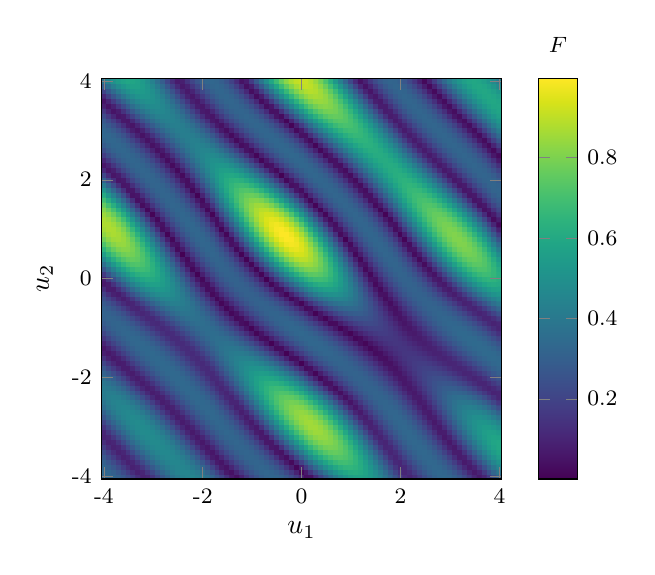
\begin{tikzpicture}[]
\begin{axis}[width=0.55\linewidth, height=0.55\linewidth, xlabel={$u_1$}, ylabel={$u_2$}, colormap/viridis, enlargelimits=false, axis on top, tick label style={font=\footnotesize}, colorbar, xtick={0,20,40,60,80}, xticklabels={-4,-2,0,2,4}, ytick={0,20,40,60,80}, yticklabels={-4,-2,0,2,4}, colorbar style={title=$F$, font=\footnotesize}]
\addplot[matrix plot*, point meta=explicit, mesh/cols=81] table[meta=z] {
x y z
0 0 0.33256
1 0 0.33624
2 0 0.32679
3 0 0.3047
4 0 0.27106
5 0 0.22769
6 0 0.1776
7 0 0.12685
8 0 0.091698
9 0 0.10201
10 0 0.1506
11 0 0.21074
12 0 0.271
13 0 0.32642
14 0 0.37396
15 0 0.41148
16 0 0.4374
17 0 0.45067
18 0 0.45071
19 0 0.43747
20 0 0.41135
21 0 0.37323
22 0 0.32445
23 0 0.26676
24 0 0.20232
25 0 0.13396
26 0 0.06708
27 0 0.039404
28 0 0.092786
29 0 0.15431
30 0 0.21026
31 0 0.25732
32 0 0.29339
33 0 0.317
34 0 0.32713
35 0 0.32326
36 0 0.30534
37 0 0.27382
38 0 0.22959
39 0 0.17402
40 0 0.10885
41 0 0.036437
42 0 0.0428
43 0 0.12327
44 0 0.20415
45 0 0.28256
46 0 0.35592
47 0 0.42184
48 0 0.47814
49 0 0.52299
50 0 0.55493
51 0 0.57293
52 0 0.57641
53 0 0.5653
54 0 0.54005
55 0 0.50157
56 0 0.45131
57 0 0.39122
58 0 0.32378
59 0 0.25235
60 0 0.18206
61 0 0.12367
62 0 0.10244
63 0 0.13206
64 0 0.18268
65 0 0.2335
66 0 0.27684
67 0 0.30923
68 0 0.32876
69 0 0.33441
70 0 0.32582
71 0 0.30326
72 0 0.26763
73 0 0.22052
74 0 0.1647
75 0 0.10636
76 0 0.069586
77 0 0.10141
78 0 0.16948
79 0 0.24406
80 0 0.31708
0 1 0.33624
1 1 0.32666
2 1 0.30439
3 1 0.27054
4 1 0.22693
5 1 0.17664
6 1 0.12582
7 1 0.091222
8 1 0.10284
9 1 0.15223
10 1 0.21274
11 1 0.27317
12 1 0.32863
13 1 0.37611
14 1 0.41346
15 1 0.43912
16 1 0.45202
17 1 0.45163
18 1 0.43787
19 1 0.4112
20 1 0.37251
21 1 0.32317
22 1 0.26498
23 1 0.2002
24 1 0.13182
25 1 0.066114
26 1 0.044158
27 1 0.097592
28 1 0.15852
29 1 0.21383
30 1 0.26004
31 1 0.29504
32 1 0.31731
33 1 0.32585
34 1 0.32012
35 1 0.3001
36 1 0.26625
37 1 0.21953
38 1 0.16132
39 1 0.09351
40 1 0.02003
41 1 0.064459
42 1 0.14763
43 1 0.23115
44 1 0.31206
45 1 0.3877
46 1 0.45563
47 1 0.51362
48 1 0.55979
49 1 0.59263
50 1 0.6111
51 1 0.61461
52 1 0.60307
53 1 0.57692
54 1 0.53709
55 1 0.48503
56 1 0.42267
57 1 0.3525
58 1 0.2777
59 1 0.20289
60 1 0.13695
61 1 0.10222
62 1 0.12255
63 1 0.17227
64 1 0.22474
65 1 0.27031
66 1 0.30494
67 1 0.32653
68 1 0.33393
69 1 0.32675
70 1 0.30522
71 1 0.27019
72 1 0.22324
73 1 0.16708
74 1 0.10768
75 1 0.068701
76 1 0.10019
77 1 0.16969
78 1 0.24593
79 1 0.32072
80 1 0.39012
0 2 0.32669
1 2 0.30431
2 2 0.27028
3 2 0.22645
4 2 0.17592
5 2 0.12498
6 2 0.090817
7 2 0.10365
8 2 0.15388
9 2 0.21487
10 2 0.27564
11 2 0.33133
12 2 0.37895
13 2 0.41634
14 2 0.44194
15 2 0.45469
16 2 0.45404
17 2 0.43996
18 2 0.41288
19 2 0.37375
20 2 0.32395
21 2 0.26532
22 2 0.20021
23 2 0.13179
24 2 0.067107
25 2 0.048307
26 2 0.10102
27 2 0.16145
28 2 0.2163
29 2 0.26193
30 2 0.29614
31 2 0.31738
32 2 0.32463
33 2 0.31735
34 2 0.29552
35 2 0.25964
36 2 0.21068
37 2 0.15009
38 2 0.079999
39 2 0.014024
40 2 0.084576
41 2 0.17042
42 2 0.25662
43 2 0.34013
44 2 0.41823
45 2 0.48837
46 2 0.54831
47 2 0.59609
48 2 0.63017
49 2 0.64946
50 2 0.65334
51 2 0.64172
52 2 0.615
53 2 0.57413
54 2 0.52055
55 2 0.45619
56 2 0.3835
57 2 0.30556
58 2 0.22657
59 2 0.15392
60 2 0.10603
61 2 0.11353
62 2 0.16078
63 2 0.21474
64 2 0.26272
65 2 0.29991
66 2 0.32392
67 2 0.3335
68 2 0.32817
69 2 0.30809
70 2 0.27409
71 2 0.22769
72 2 0.17147
73 2 0.11102
74 2 0.068157
75 2 0.0966
76 2 0.1668
77 2 0.24447
78 2 0.32094
79 2 0.39217
80 2 0.45525
0 3 0.30451
1 3 0.27037
2 3 0.22637
3 3 0.17562
4 3 0.12449
5 3 0.090569
6 3 0.10434
7 3 0.15533
8 3 0.21688
9 3 0.2781
10 3 0.33417
11 3 0.3821
12 3 0.41973
13 3 0.44547
14 3 0.45828
15 3 0.45759
16 3 0.44336
17 3 0.41606
18 3 0.37663
19 3 0.32648
20 3 0.2675
21 3 0.2021
22 3 0.13361
23 3 0.069675
24 3 0.051836
25 3 0.10322
26 3 0.16324
27 3 0.21784
28 3 0.26314
29 3 0.29686
30 3 0.3174
31 3 0.32371
32 3 0.31523
33 3 0.29196
34 3 0.25439
35 3 0.20352
36 3 0.14091
37 3 0.069122
38 3 0.02336
39 3 0.10246
40 3 0.19086
41 3 0.27972
42 3 0.36589
43 3 0.44655
44 3 0.5191
45 3 0.5812
46 3 0.63088
47 3 0.66652
48 3 0.68698
49 3 0.69162
50 3 0.68029
51 3 0.6534
52 3 0.61187
53 3 0.55712
54 3 0.49109
55 3 0.41618
56 3 0.3354
57 3 0.25264
58 3 0.17413
59 3 0.11445
60 3 0.10604
61 3 0.14847
62 3 0.20349
63 3 0.25397
64 3 0.29397
65 3 0.32077
66 3 0.33293
67 3 0.32988
68 3 0.31172
69 3 0.27921
70 3 0.23379
71 3 0.17792
72 3 0.11661
73 3 0.068725
74 3 0.090772
75 3 0.1607
76 3 0.23944
77 3 0.31742
78 3 0.39041
79 3 0.45541
80 3 0.51001
0 4 0.27089
1 4 0.22679
2 4 0.17586
3 4 0.12451
4 4 0.090558
5 4 0.10481
6 4 0.1564
7 4 0.21849
8 4 0.28024
9 4 0.33681
10 4 0.38521
11 4 0.42324
12 4 0.44933
13 4 0.46239
14 4 0.46186
15 4 0.44769
16 4 0.42035
17 4 0.38079
18 4 0.33043
19 4 0.27121
20 4 0.20556
21 4 0.13699
22 4 0.073473
23 4 0.054846
24 4 0.10436
25 4 0.16401
26 4 0.21856
27 4 0.2638
28 4 0.29733
29 4 0.31752
30 4 0.32326
31 4 0.31398
32 4 0.28967
33 4 0.25081
34 4 0.19845
35 4 0.13427
36 4 0.061629
37 4 0.035132
38 4 0.1175
39 4 0.20825
40 4 0.29967
41 4 0.38846
42 4 0.47173
43 4 0.5468
44 4 0.61127
45 4 0.66309
46 4 0.7006
47 4 0.72259
48 4 0.72836
49 4 0.71775
50 4 0.69112
51 4 0.64935
52 4 0.59385
53 4 0.52655
54 4 0.44982
55 4 0.36658
56 4 0.28049
57 4 0.19696
58 4 0.12733
59 4 0.10143
60 4 0.1357
61 4 0.19102
62 4 0.24398
63 4 0.28699
64 4 0.31687
65 4 0.33199
66 4 0.33165
67 4 0.31587
68 4 0.28532
69 4 0.24138
70 4 0.18631
71 4 0.12456
72 4 0.071404
73 4 0.08319
74 4 0.15143
75 4 0.23076
76 4 0.30997
77 4 0.38455
78 4 0.4514
79 4 0.50803
80 4 0.55244
0 5 0.22777
1 5 0.17673
2 5 0.12516
3 5 0.090857
4 5 0.105
5 5 0.15689
6 5 0.21946
7 5 0.28176
8 5 0.33891
9 5 0.38789
10 5 0.42648
11 5 0.45308
12 5 0.46658
13 5 0.46642
14 5 0.45252
15 5 0.42534
16 5 0.38583
17 5 0.33543
18 5 0.27608
19 5 0.21028
20 5 0.14162
21 5 0.078203
22 5 0.057484
23 5 0.10458
24 5 0.16388
25 5 0.21853
26 5 0.26395
27 5 0.29761
28 5 0.3178
29 5 0.32336
30 5 0.3137
31 5 0.28878
32 5 0.24909
33 5 0.19572
34 5 0.1305
35 5 0.058016
36 5 0.045219
37 5 0.12921
38 5 0.22199
39 5 0.31576
40 5 0.40707
41 5 0.49292
42 5 0.57055
43 5 0.63752
44 5 0.69168
45 5 0.73131
46 5 0.75515
47 5 0.76245
48 5 0.75297
49 5 0.72704
50 5 0.6855
51 5 0.62974
52 5 0.56164
53 5 0.48354
54 5 0.3983
55 5 0.3094
56 5 0.22163
57 5 0.14395
58 5 0.10098
59 5 0.12304
60 5 0.17744
61 5 0.2327
62 5 0.27883
63 5 0.31202
64 5 0.33041
65 5 0.33316
66 5 0.32019
67 5 0.29209
68 5 0.25012
69 5 0.1964
70 5 0.13478
71 5 0.077074
72 5 0.074839
73 5 0.13927
74 5 0.21851
75 5 0.29856
76 5 0.37446
77 5 0.44299
78 5 0.50158
79 5 0.54812
80 5 0.58104
0 6 0.1783
1 6 0.12651
2 6 0.091534
3 6 0.10484
4 6 0.15667
5 6 0.21959
6 6 0.28241
7 6 0.34017
8 6 0.3898
9 6 0.42906
10 6 0.45632
11 6 0.47044
12 6 0.47083
13 6 0.4574
14 6 0.43058
15 6 0.39132
16 6 0.34106
17 6 0.28174
18 6 0.2159
19 6 0.14717
20 6 0.083608
21 6 0.059908
22 6 0.10402
23 6 0.16293
24 6 0.21782
25 6 0.26364
26 6 0.29771
27 6 0.31823
28 6 0.324
29 6 0.31439
30 6 0.28933
31 6 0.24931
32 6 0.19545
33 6 0.12977
34 6 0.0583
35 6 0.052895
36 6 0.13729
37 6 0.23165
38 6 0.32746
39 6 0.42107
40 6 0.50936
41 6 0.58952
42 6 0.65901
43 6 0.71564
44 6 0.7576
45 6 0.78358
46 6 0.79275
47 6 0.78481
48 6 0.76003
49 6 0.71921
50 6 0.6637
51 6 0.59532
52 6 0.51638
53 6 0.42967
54 6 0.33853
55 6 0.24729
56 6 0.16322
57 6 0.10538
58 6 0.11132
59 6 0.16296
60 6 0.22016
61 6 0.26941
62 6 0.30605
63 6 0.32795
64 6 0.33411
65 6 0.32434
66 6 0.29912
67 6 0.25962
68 6 0.20778
69 6 0.14697
70 6 0.0861
71 6 0.067425
72 6 0.12471
73 6 0.20297
74 6 0.28334
75 6 0.36021
76 6 0.43016
77 6 0.49052
78 6 0.53911
79 6 0.57427
80 6 0.5948
0 7 0.1286
1 7 0.09265
2 7 0.10435
3 7 0.15564
4 7 0.21871
5 7 0.28195
6 7 0.3403
7 7 0.39062
8 7 0.43063
9 7 0.45865
10 7 0.47354
11 7 0.47465
12 7 0.46188
13 7 0.43563
14 7 0.39682
15 7 0.3469
16 7 0.28779
17 7 0.22203
18 7 0.1533
19 7 0.089443
20 7 0.062262
21 7 0.10284
22 7 0.16127
23 7 0.21648
24 7 0.26287
25 7 0.29759
26 7 0.31875
27 7 0.32511
28 7 0.31597
29 7 0.29124
30 7 0.2514
31 7 0.19758
32 7 0.13203
33 7 0.062019
34 7 0.05819
35 7 0.14163
36 7 0.23698
37 7 0.33441
38 7 0.42998
39 7 0.52048
40 7 0.60302
41 7 0.67499
42 7 0.73411
43 7 0.77854
44 7 0.80686
45 7 0.81818
46 7 0.81214
47 7 0.78895
48 7 0.74934
49 7 0.69459
50 7 0.62648
51 7 0.54728
52 7 0.4597
53 7 0.36694
54 7 0.27302
55 7 0.18399
56 7 0.11427
57 7 0.10157
58 7 0.14789
59 7 0.20649
60 7 0.25873
61 7 0.29886
62 7 0.3244
63 7 0.3342
64 7 0.32793
65 7 0.30598
66 7 0.2694
67 7 0.21997
68 7 0.16066
69 7 0.098205
70 7 0.063427
71 7 0.10861
72 7 0.1846
73 7 0.26467
74 7 0.34204
75 7 0.41304
76 7 0.47489
77 7 0.52535
78 7 0.56266
79 7 0.58555
80 7 0.59328
0 8 0.094258
1 8 0.10356
2 8 0.15376
3 8 0.21671
4 8 0.28025
5 8 0.33911
6 8 0.39009
7 8 0.43087
8 8 0.45973
9 8 0.47548
10 8 0.47745
11 8 0.4655
12 8 0.44001
13 8 0.40187
14 8 0.35248
15 8 0.29378
16 8 0.22828
17 8 0.15965
18 8 0.095464
19 8 0.064653
20 8 0.10119
21 8 0.159
22 8 0.21455
23 8 0.26163
24 8 0.29719
25 8 0.31927
26 8 0.32654
27 8 0.31827
28 8 0.29432
29 8 0.25514
30 8 0.20191
31 8 0.13703
32 8 0.068534
33 8 0.061557
34 8 0.14235
35 8 0.23795
36 8 0.33646
37 8 0.43356
38 8 0.52593
39 8 0.61059
40 8 0.68486
41 8 0.74641
42 8 0.79331
43 8 0.82409
44 8 0.83778
45 8 0.83395
46 8 0.81272
47 8 0.77476
48 8 0.72129
49 8 0.65402
50 8 0.57515
51 8 0.48732
52 8 0.39362
53 8 0.2978
54 8 0.20508
55 8 0.12642
56 8 0.094845
57 8 0.13266
58 8 0.19188
59 8 0.24688
60 8 0.29042
61 8 0.31964
62 8 0.33319
63 8 0.33064
64 8 0.31225
65 8 0.27897
66 8 0.23242
67 8 0.17523
68 8 0.11266
69 8 0.065227
70 8 0.092252
71 8 0.1641
72 8 0.24306
73 8 0.32036
74 8 0.39196
75 8 0.45495
76 8 0.50699
77 8 0.54625
78 8 0.57139
79 8 0.58158
80 8 0.57654
0 9 0.10257
1 9 0.15107
2 9 0.21358
3 9 0.27721
4 9 0.33645
5 9 0.38802
6 9 0.42953
7 9 0.45925
8 9 0.47592
9 9 0.47886
10 9 0.46788
11 9 0.44331
12 9 0.40602
13 9 0.35737
14 9 0.29927
15 9 0.23424
16 9 0.16586
17 9 0.10141
18 9 0.067128
19 9 0.099259
20 9 0.15625
21 9 0.21212
22 9 0.25994
23 9 0.29648
24 9 0.31967
25 9 0.32812
26 9 0.32105
27 9 0.29828
28 9 0.26024
29 9 0.2081
30 9 0.14438
31 9 0.077271
32 9 0.063808
33 9 0.13979
34 9 0.23474
35 9 0.33368
36 9 0.43178
37 9 0.52556
38 9 0.61197
39 9 0.68827
40 9 0.75206
41 9 0.80136
42 9 0.83461
43 9 0.85078
44 9 0.84936
45 9 0.83039
46 9 0.79448
47 9 0.74275
48 9 0.67686
49 9 0.59891
50 9 0.51147
51 9 0.41753
52 9 0.3206
53 9 0.22533
54 9 0.14026
55 9 0.091811
56 9 0.11776
57 9 0.17666
58 9 0.23409
59 9 0.28084
60 9 0.31363
61 9 0.33093
62 9 0.33219
63 9 0.31755
64 9 0.28785
65 9 0.24457
66 9 0.19005
67 9 0.12854
68 9 0.073346
69 9 0.077641
70 9 0.14235
71 9 0.21921
72 9 0.2958
73 9 0.36746
74 9 0.43112
75 9 0.48436
76 9 0.52528
77 9 0.55245
78 9 0.56498
79 9 0.56251
80 9 0.54519
0 10 0.14765
1 10 0.20936
2 10 0.27283
3 10 0.33228
4 10 0.3843
5 10 0.42647
6 10 0.45699
7 10 0.47461
8 10 0.47856
9 10 0.46863
10 10 0.44512
11 10 0.40884
12 10 0.36113
13 10 0.30385
14 10 0.23947
15 10 0.17154
16 10 0.10699
17 10 0.06966
18 10 0.09723
19 10 0.15321
20 10 0.20929
21 10 0.25784
22 10 0.29541
23 10 0.31983
24 10 0.32967
25 10 0.32408
26 10 0.30283
27 10 0.26632
28 10 0.21572
29 10 0.15357
30 10 0.087765
31 10 0.066017
32 10 0.13454
33 10 0.22777
34 10 0.32639
35 10 0.42487
36 10 0.51951
37 10 0.6072
38 10 0.68513
39 10 0.75086
40 10 0.80234
41 10 0.83795
42 10 0.8566
43 10 0.85769
44 10 0.8412
45 10 0.80764
46 10 0.75805
47 10 0.69401
48 10 0.61755
49 10 0.53113
50 10 0.43763
51 10 0.3404
52 10 0.24362
53 10 0.15418
54 10 0.092259
55 10 0.10373
56 10 0.16124
57 10 0.22068
58 10 0.27035
59 10 0.30649
60 10 0.3274
61 10 0.33242
62 10 0.32159
63 10 0.29563
64 10 0.25589
65 10 0.20448
66 10 0.14492
67 10 0.08617
68 10 0.067621
69 10 0.12052
70 10 0.19398
71 10 0.2691
72 10 0.34022
73 10 0.40402
74 10 0.458
75 10 0.50018
76 10 0.52909
77 10 0.54374
78 10 0.54369
79 10 0.52904
80 10 0.50038
0 11 0.20416
1 11 0.26719
2 11 0.32662
3 11 0.37892
4 11 0.42161
5 11 0.45285
6 11 0.47135
7 11 0.47631
8 11 0.46749
9 11 0.44512
10 11 0.40999
11 11 0.36338
12 11 0.30711
13 11 0.2436
14 11 0.17632
15 11 0.11192
16 11 0.072147
17 11 0.095292
18 11 0.15005
19 11 0.20623
20 11 0.25542
21 11 0.294
22 11 0.3197
23 11 0.33103
24 11 0.3271
25 11 0.30763
26 11 0.27298
27 11 0.22429
28 11 0.16406
29 11 0.099592
30 11 0.069304
31 11 0.12742
32 11 0.21763
33 11 0.3151
34 11 0.41325
35 11 0.50814
36 11 0.59654
37 11 0.67562
38 11 0.74287
39 11 0.7962
40 11 0.83395
41 11 0.85495
42 11 0.85854
43 11 0.84461
44 11 0.8136
45 11 0.76646
46 11 0.70468
47 11 0.63019
48 11 0.54537
49 11 0.45299
50 11 0.35621
51 11 0.25888
52 11 0.16675
53 11 0.095048
54 11 0.090983
55 11 0.14608
56 11 0.20711
57 11 0.25931
58 11 0.29845
59 11 0.3227
60 11 0.3313
61 11 0.3242
62 11 0.302
63 11 0.26594
64 11 0.21792
65 11 0.16097
66 11 0.10148
67 11 0.065048
68 11 0.10007
69 11 0.16834
70 11 0.24113
71 11 0.31106
72 11 0.37443
73 11 0.42862
74 11 0.4716
75 11 0.50183
76 11 0.51828
77 11 0.52043
78 11 0.50829
79 11 0.48239
80 11 0.44378
0 12 0.26045
1 12 0.3196
2 12 0.37195
3 12 0.41497
4 12 0.44679
5 12 0.46606
6 12 0.47198
7 12 0.46425
8 12 0.44307
9 12 0.40916
10 12 0.36378
11 12 0.30868
12 12 0.24624
13 12 0.17985
14 12 0.11588
15 12 0.074429
16 12 0.093614
17 12 0.14702
18 12 0.20312
19 12 0.25282
20 12 0.2923
21 12 0.31924
22 12 0.33209
23 12 0.32991
24 12 0.31239
25 12 0.27983
26 12 0.23332
27 12 0.1753
28 12 0.11231
29 12 0.074488
30 12 0.11941
31 12 0.20508
32 12 0.30049
33 12 0.39756
34 12 0.49201
35 12 0.5805
36 12 0.66015
37 12 0.72842
38 12 0.78318
39 12 0.82272
40 12 0.84582
41 12 0.85177
42 12 0.84037
43 12 0.81198
44 12 0.76748
45 12 0.70826
46 12 0.63615
47 12 0.55344
48 12 0.46277
49 12 0.36716
50 12 0.27017
51 12 0.17674
52 12 0.098522
53 12 0.079746
54 12 0.13171
55 12 0.19393
56 12 0.2482
57 12 0.28989
58 12 0.31708
59 12 0.32894
60 12 0.32533
61 12 0.30678
62 12 0.27439
63 12 0.22991
64 12 0.17597
65 12 0.11747
66 12 0.070333
67 12 0.082899
68 12 0.14335
69 12 0.21285
70 12 0.28089
71 12 0.34322
72 12 0.39706
73 12 0.44032
74 12 0.47141
75 12 0.48926
76 12 0.49328
77 12 0.48341
78 12 0.46011
79 12 0.42434
80 12 0.37759
0 13 0.31142
1 13 0.36357
2 13 0.4067
3 13 0.43889
4 13 0.45879
5 13 0.46555
6 13 0.45883
7 13 0.43881
8 13 0.40617
9 13 0.36209
10 13 0.3083
11 13 0.2471
12 13 0.18182
13 13 0.11861
14 13 0.076314
15 13 0.092336
16 13 0.14436
17 13 0.20019
18 13 0.25021
19 13 0.29043
20 13 0.31848
21 13 0.33278
22 13 0.33236
23 13 0.31684
24 13 0.2865
25 13 0.24237
26 13 0.18674
27 13 0.12546
28 13 0.08182
29 13 0.11165
30 13 0.19099
31 13 0.28338
32 13 0.3786
33 13 0.4719
34 13 0.55981
35 13 0.6394
36 13 0.7081
37 13 0.76376
38 13 0.80465
39 13 0.8295
40 13 0.83753
41 13 0.8285
42 13 0.80269
43 13 0.76089
44 13 0.70441
45 13 0.63498
46 13 0.55478
47 13 0.46633
48 13 0.37252
49 13 0.27667
50 13 0.18311
51 13 0.10101
52 13 0.06989
53 13 0.11867
54 13 0.1818
55 13 0.23762
56 13 0.28131
57 13 0.31092
58 13 0.32558
59 13 0.32511
60 13 0.30993
61 13 0.28106
62 13 0.24009
63 13 0.18937
64 13 0.13285
65 13 0.080839
66 13 0.071178
67 13 0.12015
68 13 0.1852
69 13 0.25065
70 13 0.31134
71 13 0.36426
72 13 0.40725
73 13 0.43868
74 13 0.45745
75 13 0.46293
76 13 0.45501
77 13 0.43406
78 13 0.40099
79 13 0.35719
80 13 0.30462
0 14 0.35403
1 14 0.397
2 14 0.42933
3 14 0.44965
4 14 0.45708
5 14 0.45126
6 14 0.43232
7 14 0.40091
8 14 0.35817
9 14 0.30576
10 14 0.24594
11 14 0.18197
12 14 0.11987
13 14 0.077623
14 14 0.091567
15 14 0.14229
16 14 0.19769
17 14 0.2478
18 14 0.28854
19 14 0.31752
20 14 0.33312
21 14 0.33434
22 14 0.3208
23 14 0.2927
24 14 0.25103
25 14 0.19793
26 14 0.13856
27 14 0.090985
28 14 0.10527
29 14 0.17632
30 14 0.26467
31 14 0.35726
32 14 0.4487
33 14 0.53535
34 14 0.61421
35 14 0.68272
36 14 0.7387
37 14 0.78041
38 14 0.80653
39 14 0.81628
40 14 0.80934
41 14 0.78593
42 14 0.74677
43 14 0.69308
44 14 0.6265
45 14 0.5491
46 14 0.46328
47 14 0.37181
48 14 0.27777
49 14 0.18506
50 14 0.10112
51 14 0.060969
52 14 0.10758
53 14 0.17141
54 14 0.22822
55 14 0.27328
56 14 0.30469
57 14 0.32159
58 14 0.32375
59 14 0.31156
60 14 0.28591
61 14 0.24827
62 14 0.20079
63 14 0.14677
64 14 0.093391
65 14 0.066493
66 14 0.099883
67 14 0.15911
68 14 0.22128
69 14 0.27973
70 14 0.33117
71 14 0.37334
72 14 0.4046
73 14 0.42379
74 14 0.43028
75 14 0.42389
76 14 0.40497
77 14 0.37435
78 14 0.33337
79 14 0.28393
80 14 0.22867
0 15 0.38617
1 15 0.41839
2 15 0.43888
3 15 0.44676
4 15 0.44166
5 15 0.42368
6 15 0.39342
7 15 0.35199
8 15 0.30098
9 15 0.24263
10 15 0.18014
11 15 0.11948
12 15 0.078231
13 15 0.091394
14 15 0.14104
15 15 0.19586
16 15 0.24581
17 15 0.28683
18 15 0.31648
19 15 0.33316
20 15 0.33586
21 15 0.32416
22 15 0.29823
23 15 0.259
24 15 0.20847
25 15 0.15119
26 15 0.10133
27 15 0.10119
28 15 0.162
29 15 0.24526
30 15 0.33449
31 15 0.4234
32 15 0.50812
33 15 0.5856
34 15 0.65326
35 15 0.70894
36 15 0.75087
37 15 0.77775
38 15 0.78874
39 15 0.7835
40 15 0.76221
41 15 0.7255
42 15 0.67452
43 15 0.61082
44 15 0.53638
45 15 0.45348
46 15 0.36474
47 15 0.27308
48 15 0.18203
49 15 0.097823
50 15 0.052428
51 15 0.099159
52 15 0.16351
53 15 0.2207
54 15 0.26642
55 15 0.29894
56 15 0.31742
57 15 0.32163
58 15 0.31188
59 15 0.28903
60 15 0.25442
61 15 0.21001
62 15 0.15867
63 15 0.10579
64 15 0.068266
65 15 0.083638
66 15 0.13536
67 15 0.19358
68 15 0.2493
69 15 0.29875
70 15 0.33959
71 15 0.37014
72 15 0.38925
73 15 0.39625
74 15 0.39097
75 15 0.3737
76 15 0.34524
77 15 0.30688
78 15 0.26049
79 15 0.20878
80 15 0.15611
0 16 0.40639
1 16 0.42679
2 16 0.43489
3 16 0.43029
4 16 0.41307
5 16 0.38383
6 16 0.34361
7 16 0.29399
8 16 0.23715
9 16 0.17627
10 16 0.11738
11 16 0.078108
12 16 0.091899
13 16 0.14079
14 16 0.19491
15 16 0.24448
16 16 0.28548
17 16 0.31553
18 16 0.33301
19 16 0.33694
20 16 0.32687
21 16 0.30296
22 16 0.26606
23 16 0.21805
24 16 0.16296
25 16 0.11212
26 16 0.099879
27 16 0.14892
28 16 0.22606
29 16 0.31122
30 16 0.39697
31 16 0.47915
32 16 0.55463
33 16 0.62081
34 16 0.67555
35 16 0.7171
36 16 0.74415
37 16 0.75586
38 16 0.75186
39 16 0.73229
40 16 0.69773
41 16 0.64926
42 16 0.58836
43 16 0.5169
44 16 0.43706
45 16 0.35134
46 16 0.26248
47 16 0.17372
48 16 0.090455
49 16 0.044089
50 16 0.094245
51 16 0.15881
52 16 0.2157
53 16 0.26135
54 16 0.29424
55 16 0.31357
56 16 0.31914
57 16 0.31123
58 16 0.29063
59 16 0.25861
60 16 0.21697
61 16 0.16826
62 16 0.11677
63 16 0.073881
64 16 0.072142
65 16 0.11459
66 16 0.16824
67 16 0.2208
68 16 0.26785
69 16 0.30691
70 16 0.33628
71 16 0.35482
72 16 0.36187
73 16 0.35723
74 16 0.34121
75 16 0.31457
76 16 0.27859
77 16 0.23518
78 16 0.18718
79 16 0.13953
80 16 0.10291
0 17 0.41377
1 17 0.42181
2 17 0.41746
3 17 0.40079
4 17 0.37237
5 17 0.33323
6 17 0.28491
7 17 0.22957
8 17 0.17039
9 17 0.11359
10 17 0.077353
11 17 0.093179
12 17 0.14168
13 17 0.19502
14 17 0.24398
15 17 0.28469
16 17 0.31482
17 17 0.33281
18 17 0.33767
19 17 0.32896
20 17 0.30682
21 17 0.27206
22 17 0.22644
23 17 0.17356
24 17 0.1227
25 17 0.10121
26 17 0.13777
27 17 0.20785
28 17 0.28833
29 17 0.3704
30 17 0.44949
31 17 0.5224
32 17 0.58652
33 17 0.63972
34 17 0.68028
35 17 0.7069
36 17 0.71876
37 17 0.71548
38 17 0.69716
39 17 0.66437
40 17 0.61811
41 17 0.5598
42 17 0.49122
43 17 0.41446
44 17 0.3319
45 17 0.24613
46 17 0.16013
47 17 0.078721
48 17 0.037054
49 17 0.09373
50 17 0.1579
51 17 0.21375
52 17 0.25858
53 17 0.29107
54 17 0.31052
55 17 0.31673
56 17 0.30999
57 17 0.29103
58 17 0.26106
59 17 0.22176
60 17 0.17543
61 17 0.12567
62 17 0.080598
63 17 0.065334
64 17 0.097138
65 17 0.14574
66 17 0.19485
67 17 0.23919
68 17 0.27611
69 17 0.30391
70 17 0.32144
71 17 0.32809
72 17 0.32367
73 17 0.30849
74 17 0.28333
75 17 0.2495
76 17 0.20902
77 17 0.16505
78 17 0.12349
79 17 0.097095
80 17 0.103
0 18 0.40794
1 18 0.40356
2 18 0.38719
3 18 0.35938
4 18 0.32113
5 18 0.27399
6 18 0.22007
7 18 0.16265
8 18 0.10826
9 18 0.076212
10 18 0.09534
11 18 0.14378
12 18 0.19628
13 18 0.24444
14 18 0.2846
15 18 0.31452
16 18 0.33269
17 18 0.33815
18 18 0.33048
19 18 0.30983
20 18 0.27696
21 18 0.23352
22 18 0.18279
23 18 0.13254
24 18 0.10456
25 18 0.12903
26 18 0.1913
27 18 0.26661
28 18 0.34456
29 18 0.42013
30 18 0.48998
31 18 0.55151
32 18 0.60262
33 18 0.64161
34 18 0.66723
35 18 0.67867
36 18 0.67555
37 18 0.65798
38 18 0.6265
39 18 0.58207
40 18 0.52605
41 18 0.46015
42 18 0.38637
43 18 0.30698
44 18 0.22444
45 18 0.14151
46 18 0.062675
47 18 0.034917
48 18 0.098249
49 18 0.16112
50 18 0.21519
51 18 0.25847
52 18 0.28983
53 18 0.30866
54 18 0.31479
55 18 0.30851
56 18 0.29053
57 18 0.26202
58 18 0.22454
59 18 0.18023
60 18 0.1322
61 18 0.086599
62 18 0.062113
63 18 0.083004
64 18 0.12629
65 18 0.17184
66 18 0.21331
67 18 0.24785
68 18 0.27376
69 18 0.28994
70 18 0.2958
71 18 0.29122
72 18 0.27652
73 18 0.25254
74 18 0.22069
75 18 0.1832
76 18 0.14383
77 18 0.11003
78 18 0.096188
79 18 0.1129
80 18 0.14937
0 19 0.38904
1 19 0.3727
2 19 0.34524
3 19 0.30768
4 19 0.26153
5 19 0.20894
6 19 0.15329
7 19 0.10167
8 19 0.075067
9 19 0.098483
10 19 0.14711
11 19 0.19873
12 19 0.24593
13 19 0.28529
14 19 0.31471
15 19 0.33274
16 19 0.33847
17 19 0.33152
18 19 0.31202
19 19 0.28072
20 19 0.23922
21 19 0.1905
22 19 0.14125
23 19 0.10909
24 19 0.12282
25 19 0.1769
26 19 0.24669
27 19 0.32022
28 19 0.39193
29 19 0.45835
30 19 0.51686
31 19 0.5654
32 19 0.60231
33 19 0.62639
34 19 0.63685
35 19 0.63336
36 19 0.61602
37 19 0.58536
38 19 0.54232
39 19 0.48821
40 19 0.4247
41 19 0.3537
42 19 0.27738
43 19 0.19808
44 19 0.1184
45 19 0.04276
46 19 0.041895
47 19 0.10786
48 19 0.16847
49 19 0.22007
50 19 0.26114
51 19 0.29071
52 19 0.30823
53 19 0.31359
54 19 0.30709
55 19 0.28944
56 19 0.26175
57 19 0.22555
58 19 0.1828
59 19 0.13627
60 19 0.090908
61 19 0.06075
62 19 0.071808
63 19 0.1099
64 19 0.15198
65 19 0.19055
66 19 0.22259
67 19 0.24641
68 19 0.26098
69 19 0.26576
70 19 0.26069
71 19 0.24618
72 19 0.22316
73 19 0.19323
74 19 0.159
75 19 0.12526
76 19 0.10145
77 19 0.1012
78 19 0.12627
79 19 0.16426
80 19 0.20533
0 20 0.35777
1 20 0.3304
2 20 0.29328
3 20 0.24792
4 20 0.19652
5 20 0.14264
6 20 0.09421
7 20 0.074391
8 20 0.10267
9 20 0.1516
10 20 0.20231
11 20 0.24841
12 20 0.28679
13 20 0.31545
14 20 0.33304
15 20 0.33871
16 20 0.33212
17 20 0.31343
18 20 0.28339
19 20 0.24351
20 20 0.19662
21 20 0.14858
22 20 0.11398
23 20 0.11895
24 20 0.16495
25 20 0.22907
26 20 0.29801
27 20 0.36565
28 20 0.42837
29 20 0.48353
30 20 0.52911
31 20 0.56351
32 20 0.58557
33 20 0.59457
34 20 0.59019
35 20 0.57256
36 20 0.54222
37 20 0.50011
38 20 0.44751
39 20 0.38602
40 20 0.31752
41 20 0.24408
42 20 0.16794
43 20 0.091546
44 20 0.020333
45 20 0.057378
46 20 0.12199
47 20 0.17958
48 20 0.22817
49 20 0.26649
50 20 0.29369
51 20 0.3093
52 20 0.31326
53 20 0.30591
54 20 0.28795
55 20 0.26049
56 20 0.22498
57 20 0.1833
58 20 0.13795
59 20 0.093072
60 20 0.059624
61 20 0.062861
62 20 0.096368
63 20 0.13529
64 20 0.17109
65 20 0.20062
66 20 0.22225
67 20 0.23503
68 20 0.23851
69 20 0.23272
70 20 0.21819
71 20 0.19602
72 20 0.1681
73 20 0.13774
74 20 0.11118
75 20 0.099416
76 20 0.11148
77 20 0.14206
78 20 0.18049
79 20 0.21991
80 20 0.2564
0 21 0.31532
1 21 0.27838
2 21 0.23358
3 21 0.1832
4 21 0.13106
5 21 0.086354
6 21 0.074651
7 21 0.10786
8 21 0.15711
9 21 0.20689
10 21 0.2518
11 21 0.28901
12 21 0.31669
13 21 0.33357
14 21 0.33888
15 21 0.33233
16 21 0.3141
17 21 0.28497
18 21 0.24642
19 21 0.20111
20 21 0.15437
21 21 0.1186
22 21 0.11698
23 21 0.15552
24 21 0.21407
25 21 0.27841
26 21 0.3419
27 21 0.40076
28 21 0.45235
29 21 0.49469
30 21 0.52623
31 21 0.54588
32 21 0.55297
33 21 0.54724
34 21 0.52886
35 21 0.49837
36 21 0.45673
37 21 0.40519
38 21 0.34535
39 21 0.27902
40 21 0.2082
41 21 0.13505
42 21 0.061873
43 21 0.012986
44 21 0.078172
45 21 0.13969
46 21 0.19379
47 21 0.23897
48 21 0.27413
49 21 0.2985
50 21 0.31171
51 21 0.31375
52 21 0.30498
53 21 0.28615
54 21 0.25835
55 21 0.22299
56 21 0.18188
57 21 0.13733
58 21 0.092913
59 21 0.057595
60 21 0.05537
61 21 0.085419
62 21 0.12171
63 21 0.15497
64 21 0.18208
65 21 0.2015
66 21 0.21239
67 21 0.21443
68 21 0.20776
69 21 0.19308
70 21 0.17174
71 21 0.14612
72 21 0.12057
73 21 0.10302
74 21 0.10384
75 21 0.12525
76 21 0.15906
77 21 0.19725
78 21 0.2349
79 21 0.26896
80 21 0.29733
0 22 0.26342
1 22 0.21895
2 22 0.16939
3 22 0.11896
4 22 0.078667
5 22 0.076184
6 22 0.11396
7 22 0.16343
8 22 0.21226
9 22 0.2559
10 22 0.29182
11 22 0.31833
12 22 0.33427
13 22 0.33895
14 22 0.33212
15 22 0.31403
16 22 0.28547
17 22 0.24792
18 22 0.20397
19 22 0.15851
20 22 0.12247
21 22 0.11634
22 22 0.14854
23 22 0.20187
24 22 0.26174
25 22 0.32112
26 22 0.37608
27 22 0.42399
28 22 0.4629
29 22 0.49133
30 22 0.50827
31 22 0.5131
32 22 0.50563
33 22 0.48607
34 22 0.45501
35 22 0.4134
36 22 0.36252
37 22 0.30392
38 22 0.2394
39 22 0.1709
40 22 0.1005
41 22 0.030432
42 22 0.038183
43 22 0.10193
44 22 0.15983
45 22 0.21021
46 22 0.25176
47 22 0.28347
48 22 0.30469
49 22 0.3151
50 22 0.31477
51 22 0.30413
52 22 0.28394
53 22 0.2553
54 22 0.21961
55 22 0.17862
56 22 0.13447
57 22 0.090371
58 22 0.053987
59 22 0.048698
60 22 0.076876
61 22 0.11118
62 22 0.1422
63 22 0.16702
64 22 0.18425
65 22 0.1932
66 22 0.19368
67 22 0.18602
68 22 0.17111
69 22 0.15068
70 22 0.12783
71 22 0.10825
72 22 0.10097
73 22 0.11285
74 22 0.14056
75 22 0.17614
76 22 0.21373
77 22 0.24962
78 22 0.28134
79 22 0.30707
80 22 0.32548
0 23 0.20444
1 23 0.1555
2 23 0.10677
3 23 0.071742
4 23 0.079091
5 23 0.12074
6 23 0.1703
7 23 0.21816
8 23 0.26048
9 23 0.29501
10 23 0.3202
11 23 0.33501
12 23 0.3388
13 23 0.33142
14 23 0.31316
15 23 0.28487
16 23 0.24802
17 23 0.20516
18 23 0.16096
19 23 0.12531
20 23 0.11651
21 23 0.1438
22 23 0.19251
23 23 0.24822
24 23 0.30364
25 23 0.35477
26 23 0.39898
27 23 0.43436
28 23 0.45953
29 23 0.47353
30 23 0.47584
31 23 0.46631
32 23 0.44523
33 23 0.41321
34 23 0.37124
35 23 0.32062
36 23 0.2629
37 23 0.19983
38 23 0.13333
39 23 0.065422
40 23 0.0027831
41 23 0.066746
42 23 0.12707
43 23 0.18128
44 23 0.22788
45 23 0.26568
46 23 0.29377
47 23 0.3116
48 23 0.31893
49 23 0.31591
50 23 0.30302
51 23 0.28106
52 23 0.25117
53 23 0.21474
54 23 0.17345
55 23 0.12937
56 23 0.085388
57 23 0.048422
58 23 0.042645
59 23 0.070836
60 23 0.1038
61 23 0.13285
62 23 0.15548
63 23 0.17054
64 23 0.17749
65 23 0.17631
66 23 0.16752
67 23 0.15231
68 23 0.13288
69 23 0.11332
70 23 0.10072
71 23 0.10365
72 23 0.12406
73 23 0.15583
74 23 0.19235
75 23 0.22919
76 23 0.26342
77 23 0.29293
78 23 0.31615
79 23 0.33191
80 23 0.33941
0 24 0.14189
1 24 0.094848
2 24 0.066129
3 24 0.083216
4 24 0.12791
5 24 0.17742
6 24 0.22429
7 24 0.26526
8 24 0.29833
9 24 0.32209
10 24 0.33559
11 24 0.33829
12 24 0.33011
13 24 0.31142
14 24 0.28309
15 24 0.24666
16 24 0.20467
17 24 0.16166
18 24 0.12695
19 24 0.1171
20 24 0.14105
21 24 0.18596
22 24 0.23795
23 24 0.28968
24 24 0.33712
25 24 0.37769
26 24 0.40954
27 24 0.43137
28 24 0.4423
29 24 0.44189
30 24 0.43007
31 24 0.40717
32 24 0.37389
33 24 0.33123
34 24 0.28053
35 24 0.22332
36 24 0.16138
37 24 0.096579
38 24 0.030885
39 24 0.033786
40 24 0.095455
41 24 0.15238
42 24 0.20296
43 24 0.24581
44 24 0.27982
45 24 0.30421
46 24 0.31848
47 24 0.32253
48 24 0.31657
49 24 0.30114
50 24 0.27711
51 24 0.24563
52 24 0.20811
53 24 0.16621
54 24 0.1219
55 24 0.07785
56 24 0.040698
57 24 0.037803
58 24 0.067804
59 24 0.099852
60 24 0.1271
61 24 0.14761
62 24 0.16045
63 24 0.1653
64 24 0.16231
65 24 0.1522
66 24 0.13651
67 24 0.11809
68 24 0.10218
69 24 0.097009
70 24 0.10891
71 24 0.13546
72 24 0.16992
73 24 0.20694
74 24 0.24303
75 24 0.27573
76 24 0.30321
77 24 0.32407
78 24 0.33728
79 24 0.34217
80 24 0.33841
0 25 0.083548
1 25 0.062226
2 25 0.088222
3 25 0.13519
4 25 0.18451
5 25 0.23036
6 25 0.26997
7 25 0.30153
8 25 0.32376
9 25 0.3358
10 25 0.33723
11 25 0.32803
12 25 0.30864
13 25 0.28002
14 25 0.24376
15 25 0.20243
16 25 0.16061
17 25 0.1273
18 25 0.11785
19 25 0.14008
20 25 0.18217
21 25 0.23098
22 25 0.27934
23 25 0.32332
24 25 0.36038
25 25 0.38877
26 25 0.40725
27 25 0.41504
28 25 0.41178
29 25 0.3975
30 25 0.37257
31 25 0.33777
32 25 0.29416
33 25 0.24307
34 25 0.18609
35 25 0.12497
36 25 0.061574
37 25 0.0023714
38 25 0.064377
39 25 0.12316
40 25 0.17685
41 25 0.22391
42 25 0.26306
43 25 0.2933
44 25 0.31392
45 25 0.32457
46 25 0.32519
47 25 0.3161
48 25 0.29791
49 25 0.27156
50 25 0.23823
51 25 0.19935
52 25 0.15658
53 25 0.1118
54 25 0.067545
55 25 0.030827
56 25 0.035983
57 25 0.06864
58 25 0.099846
59 25 0.12531
60 25 0.14363
61 25 0.15417
62 25 0.15674
63 25 0.15168
64 25 0.13995
65 25 0.12345
66 25 0.10581
67 25 0.09362
68 25 0.095571
69 25 0.11474
70 25 0.14572
71 25 0.18208
72 25 0.21941
73 25 0.2548
74 25 0.28611
75 25 0.31173
76 25 0.33039
77 25 0.34119
78 25 0.34357
79 25 0.33731
80 25 0.32251
0 26 0.060156
1 26 0.093697
2 26 0.14228
3 26 0.19129
4 26 0.23611
5 26 0.27434
6 26 0.30434
7 26 0.32496
8 26 0.33543
9 26 0.33542
10 26 0.325
11 26 0.30469
12 26 0.27554
13 26 0.2392
14 26 0.19838
15 26 0.15776
16 26 0.12639
17 26 0.1187
18 26 0.14079
19 26 0.18107
20 26 0.22731
21 26 0.27271
22 26 0.3135
23 26 0.34723
24 26 0.37226
25 26 0.38744
26 26 0.39208
27 26 0.38591
28 26 0.36903
29 26 0.34193
30 26 0.30541
31 26 0.2606
32 26 0.20889
33 26 0.15188
34 26 0.091323
35 26 0.029108
36 26 0.033011
37 26 0.09294
38 26 0.14903
39 26 0.19962
40 26 0.24327
41 26 0.2788
42 26 0.30529
43 26 0.32214
44 26 0.32909
45 26 0.32618
46 26 0.31382
47 26 0.29271
48 26 0.26384
49 26 0.22845
50 26 0.188
51 26 0.14414
52 26 0.098726
53 26 0.054163
54 26 0.01979
55 26 0.03982
56 26 0.07425
57 26 0.10434
58 26 0.12788
59 26 0.14391
60 26 0.15196
61 26 0.15202
62 26 0.14456
63 26 0.13077
64 26 0.11293
65 26 0.095518
66 26 0.086627
67 26 0.094873
68 26 0.11976
69 26 0.15407
70 26 0.19188
71 26 0.22945
72 26 0.26422
73 26 0.29431
74 26 0.31822
75 26 0.33483
76 26 0.34335
77 26 0.34331
78 26 0.3346
79 26 0.31744
80 26 0.29241
0 27 0.099246
1 27 0.14893
2 27 0.19754
3 27 0.24133
4 27 0.27817
5 27 0.30658
6 27 0.3255
7 27 0.33428
8 27 0.33267
9 27 0.32084
10 27 0.2994
11 27 0.26948
12 27 0.23288
13 27 0.19243
14 27 0.15312
15 27 0.12435
16 27 0.11979
17 27 0.14318
18 27 0.18266
19 27 0.22696
20 27 0.26983
21 27 0.30773
22 27 0.33835
23 27 0.36016
24 27 0.37212
25 27 0.37363
26 27 0.36451
27 27 0.34497
28 27 0.31556
29 27 0.27717
30 27 0.23099
31 27 0.17845
32 27 0.12119
33 27 0.060992
34 27 0.0027151
35 27 0.060976
36 27 0.11886
37 27 0.17241
38 27 0.22005
39 27 0.2604
40 27 0.29237
41 27 0.31514
42 27 0.3282
43 27 0.33139
44 27 0.32488
45 27 0.30913
46 27 0.28494
47 27 0.25338
48 27 0.21575
49 27 0.17355
50 27 0.12844
51 27 0.082239
52 27 0.037338
53 27 0.015328
54 27 0.050679
55 27 0.085198
56 27 0.1138
57 27 0.13524
58 27 0.14881
59 27 0.15419
60 27 0.15146
61 27 0.14124
62 27 0.12485
63 27 0.10491
64 27 0.08677
65 27 0.080274
66 27 0.093746
67 27 0.12317
68 27 0.16014
69 27 0.19917
70 27 0.23697
71 27 0.27123
72 27 0.30021
73 27 0.32256
74 27 0.33725
75 27 0.34358
76 27 0.34121
77 27 0.33012
78 27 0.31063
79 27 0.28345
80 27 0.24964
0 28 0.15498
1 28 0.20313
2 28 0.24588
3 28 0.28132
4 28 0.30809
5 28 0.32524
6 28 0.33221
7 28 0.32886
8 28 0.31543
9 28 0.29264
10 28 0.26175
11 28 0.22468
12 28 0.18453
13 28 0.14676
14 28 0.12144
15 28 0.12147
16 28 0.14744
17 28 0.187
18 28 0.22997
19 28 0.27074
20 28 0.30606
21 28 0.33381
22 28 0.35256
23 28 0.36139
24 28 0.35981
25 28 0.34774
26 28 0.32548
27 28 0.29366
28 28 0.25327
29 28 0.20556
30 28 0.15201
31 28 0.094319
32 28 0.034376
33 28 0.026724
34 28 0.085741
35 28 0.14175
36 28 0.19291
37 28 0.23771
38 28 0.27485
39 28 0.3033
40 28 0.32236
41 28 0.33162
42 28 0.331
43 28 0.32077
44 28 0.30151
45 28 0.2741
46 28 0.23969
47 28 0.19965
48 28 0.15553
49 28 0.10901
50 28 0.061898
51 28 0.016841
52 28 0.029282
53 28 0.068083
54 28 0.10165
55 28 0.12851
56 28 0.14772
57 28 0.1587
58 28 0.16122
59 28 0.15546
60 28 0.14211
61 28 0.12256
62 28 0.099631
63 28 0.079412
64 28 0.073879
65 28 0.091456
66 28 0.12459
67 28 0.16382
68 28 0.20398
69 28 0.24205
70 28 0.27589
71 28 0.3039
72 28 0.3248
73 28 0.33767
74 28 0.34191
75 28 0.33726
76 28 0.32382
77 28 0.30204
78 28 0.27273
79 28 0.23714
80 28 0.19702
0 29 0.20797
1 29 0.2497
2 29 0.28374
3 29 0.30883
4 29 0.32414
5 29 0.32919
6 29 0.32392
7 29 0.30869
8 29 0.28435
9 29 0.25225
10 29 0.21454
11 29 0.17467
12 29 0.13884
13 29 0.11818
14 29 0.12427
15 29 0.15386
16 29 0.19423
17 29 0.23641
18 29 0.2755
19 29 0.30855
20 29 0.33366
21 29 0.34952
22 29 0.35533
23 29 0.35071
24 29 0.33568
25 29 0.31064
26 29 0.27634
27 29 0.23382
28 29 0.18442
29 29 0.1297
30 29 0.071429
31 29 0.012244
32 29 0.049209
33 29 0.10714
34 29 0.16142
35 29 0.21033
36 29 0.25239
37 29 0.28639
38 29 0.31137
39 29 0.32671
40 29 0.33212
41 29 0.32761
42 29 0.31356
43 29 0.29065
44 29 0.25986
45 29 0.22243
46 29 0.17979
47 29 0.13356
48 29 0.085466
49 29 0.037308
50 29 0.0099722
51 29 0.052852
52 29 0.091295
53 29 0.12359
54 29 0.14861
55 29 0.16553
56 29 0.17383
57 29 0.17336
58 29 0.16437
59 29 0.14759
60 29 0.12442
61 29 0.097639
62 29 0.07371
63 29 0.067086
64 29 0.087609
65 29 0.12391
66 29 0.16522
67 29 0.2065
68 29 0.24491
69 29 0.27845
70 29 0.30559
71 29 0.32515
72 29 0.33629
73 29 0.33849
74 29 0.3316
75 29 0.31583
76 29 0.29174
77 29 0.26033
78 29 0.22302
79 29 0.18195
80 29 0.14052
0 30 0.25279
1 30 0.28544
2 30 0.30884
3 30 0.32223
4 30 0.32523
5 30 0.31789
6 30 0.30067
7 30 0.27453
8 30 0.241
9 30 0.20248
10 30 0.16294
11 30 0.12972
12 30 0.11533
13 30 0.1289
14 30 0.16282
15 30 0.20453
16 30 0.24638
17 30 0.28415
18 30 0.31524
19 30 0.33794
20 30 0.35108
21 30 0.35397
22 30 0.34636
23 30 0.32837
24 30 0.30051
25 30 0.26361
26 30 0.21884
27 30 0.1676
28 30 0.11154
29 30 0.052553
30 30 0.010355
31 30 0.068197
32 30 0.12518
33 30 0.17791
34 30 0.22469
35 30 0.26412
36 30 0.29503
37 30 0.31656
38 30 0.32817
39 30 0.32966
40 30 0.32117
41 30 0.30317
42 30 0.27645
43 30 0.24209
44 30 0.20142
45 30 0.15597
46 30 0.10743
47 30 0.057559
48 30 0.0081847
49 30 0.038984
50 30 0.082205
51 30 0.11998
52 30 0.15101
53 30 0.1742
54 30 0.18881
55 30 0.19439
56 30 0.19084
57 30 0.17848
58 30 0.15806
59 30 0.13093
60 30 0.099676
61 30 0.070447
62 30 0.05992
63 30 0.082027
64 30 0.12115
65 30 0.16449
66 30 0.20697
67 30 0.24586
68 30 0.27924
69 30 0.30564
70 30 0.32397
71 30 0.33344
72 30 0.33365
73 30 0.32452
74 30 0.30639
75 30 0.27998
76 30 0.24645
77 30 0.20752
78 30 0.16587
79 30 0.12618
80 30 0.097997
0 31 0.28654
1 31 0.30824
2 31 0.31966
3 31 0.32051
4 31 0.31093
5 31 0.2915
6 31 0.26332
7 31 0.22811
8 31 0.18861
9 31 0.14957
10 31 0.12004
11 31 0.11396
12 31 0.13611
13 31 0.17468
14 31 0.21808
15 31 0.25996
16 31 0.29676
17 31 0.32618
18 31 0.3467
19 31 0.35728
20 31 0.35737
21 31 0.34681
22 31 0.32585
23 31 0.2951
24 31 0.2555
25 31 0.20832
26 31 0.15506
27 31 0.097469
28 31 0.037667
29 31 0.025002
30 31 0.083787
31 31 0.14002
32 31 0.19137
33 31 0.23618
34 31 0.27309
35 31 0.30099
36 31 0.31909
37 31 0.32695
38 31 0.32447
39 31 0.31188
40 31 0.28977
41 31 0.25904
42 31 0.22089
43 31 0.17675
44 31 0.12823
45 31 0.077116
46 31 0.025238
47 31 0.025584
48 31 0.073488
49 31 0.11682
50 31 0.15406
51 31 0.18392
52 31 0.20536
53 31 0.21769
54 31 0.22052
55 31 0.21383
56 31 0.19799
57 31 0.17377
58 31 0.14251
59 31 0.10646
60 31 0.070859
61 31 0.052934
62 31 0.074645
63 31 0.11637
64 31 0.16183
65 31 0.20568
66 31 0.24523
67 31 0.27863
68 31 0.30447
69 31 0.32169
70 31 0.32958
71 31 0.32782
72 31 0.31646
73 31 0.29593
74 31 0.26713
75 31 0.23144
76 31 0.19098
77 31 0.14928
78 31 0.11314
79 31 0.096007
80 31 0.10928
0 32 0.30722
1 32 0.31664
2 32 0.31525
3 32 0.30328
4 32 0.28144
5 32 0.25096
6 32 0.2138
7 32 0.17317
8 32 0.13496
9 32 0.11081
10 32 0.11534
11 32 0.14652
12 32 0.18972
13 32 0.23501
14 32 0.27723
15 32 0.31335
16 32 0.34139
17 32 0.35995
18 32 0.36815
19 32 0.36554
20 32 0.35208
21 32 0.32813
22 32 0.29442
23 32 0.252
24 32 0.20224
25 32 0.14675
26 32 0.087392
27 32 0.026729
28 32 0.037047
29 32 0.096172
30 32 0.1519
31 32 0.20209
32 32 0.24512
33 32 0.27966
34 32 0.30465
35 32 0.31938
36 32 0.32348
37 32 0.31696
38 32 0.30015
39 32 0.27377
40 32 0.23884
41 32 0.19665
42 32 0.14874
43 32 0.096864
44 32 0.042865
45 32 0.011421
46 32 0.063885
47 32 0.11284
48 32 0.15654
49 32 0.19345
50 32 0.22231
51 32 0.24212
52 32 0.25223
53 32 0.25231
54 32 0.24243
55 32 0.22302
56 32 0.19491
57 32 0.15939
58 32 0.11848
59 32 0.076247
60 32 0.04758
61 32 0.065467
62 32 0.10959
63 32 0.15736
64 32 0.20284
65 32 0.24334
66 32 0.27702
67 32 0.30251
68 32 0.31879
69 32 0.32522
70 32 0.32156
71 32 0.30795
72 32 0.28497
73 32 0.25368
74 32 0.21575
75 32 0.17386
76 32 0.13284
77 32 0.10292
78 32 0.10062
79 32 0.12823
80 32 0.16982
0 33 0.31347
1 33 0.30978
2 33 0.2953
3 33 0.27084
4 33 0.23779
5 33 0.19841
6 33 0.15651
7 33 0.11976
8 33 0.10348
9 33 0.12054
10 33 0.16046
11 33 0.20805
12 33 0.25532
13 33 0.29814
14 33 0.3339
15 33 0.36083
16 33 0.37769
17 33 0.38369
18 33 0.37851
19 33 0.36221
20 33 0.33526
21 33 0.2985
22 33 0.25311
23 33 0.20058
24 33 0.14262
25 33 0.081222
26 33 0.019656
27 33 0.045924
28 33 0.10557
29 33 0.16109
30 33 0.21041
31 33 0.25192
32 33 0.28428
33 33 0.30652
34 33 0.31797
35 33 0.31835
36 33 0.30775
37 33 0.28664
38 33 0.25583
39 33 0.21646
40 33 0.16996
41 33 0.118
42 33 0.062414
43 33 0.0052306
44 33 0.051768
45 33 0.10635
46 33 0.1567
47 33 0.20108
48 33 0.23795
49 33 0.26604
50 33 0.28439
51 33 0.29239
52 33 0.28979
53 33 0.27671
54 33 0.25366
55 33 0.22155
56 33 0.18169
57 33 0.13593
58 33 0.087418
59 33 0.04657
60 33 0.05464
61 33 0.10075
62 33 0.15112
63 33 0.1986
64 33 0.24041
65 33 0.27472
66 33 0.30016
67 33 0.31575
68 33 0.3209
69 33 0.31544
70 33 0.29961
71 33 0.27412
72 33 0.24023
73 33 0.19994
74 33 0.15668
75 33 0.11735
76 33 0.097022
77 33 0.11143
78 33 0.15085
79 33 0.19854
80 33 0.24604
0 34 0.30448
1 34 0.28741
2 34 0.26016
3 34 0.2243
4 34 0.18239
5 34 0.13912
6 34 0.10492
7 34 0.099729
8 34 0.13012
9 34 0.17787
10 34 0.22952
11 34 0.27889
12 34 0.32256
13 34 0.35827
14 34 0.3844
15 34 0.39982
16 34 0.40384
17 34 0.39624
18 34 0.37717
19 34 0.34723
20 34 0.30736
21 34 0.25887
22 34 0.20335
23 34 0.14266
24 34 0.078895
25 34 0.016141
26 34 0.051682
27 34 0.11218
28 34 0.16787
29 34 0.21668
30 34 0.25697
31 34 0.28746
32 34 0.30716
33 34 0.31549
34 34 0.31225
35 34 0.2976
36 34 0.27213
37 34 0.23676
38 34 0.19276
39 34 0.14169
40 34 0.085348
41 34 0.02569
42 34 0.035219
43 34 0.095247
44 34 0.15233
45 34 0.2045
46 34 0.24996
47 34 0.28715
48 34 0.31479
49 34 0.33194
50 34 0.33802
51 34 0.33284
52 34 0.31661
53 34 0.28991
54 34 0.25374
55 34 0.20945
56 34 0.15884
57 34 0.10451
58 34 0.052848
59 34 0.042816
60 34 0.089717
61 34 0.14304
62 34 0.19297
63 34 0.23656
64 34 0.27194
65 34 0.29773
66 34 0.31297
67 34 0.31711
68 34 0.31003
69 34 0.29207
70 34 0.26405
71 34 0.22743
72 34 0.1846
73 34 0.13996
74 34 0.10358
75 34 0.096277
76 34 0.12666
77 34 0.17549
78 34 0.22847
79 34 0.2793
80 34 0.32454
0 35 0.28005
1 35 0.2499
2 35 0.21101
3 35 0.16629
4 35 0.1216
5 35 0.091687
6 35 0.10088
7 35 0.14382
8 35 0.19832
9 35 0.25377
10 35 0.30536
11 35 0.35019
12 35 0.3862
13 35 0.41187
14 35 0.42616
15 35 0.42847
16 35 0.41864
17 35 0.39693
18 35 0.36403
19 35 0.32101
20 35 0.26929
21 35 0.21059
22 35 0.14688
23 35 0.080393
24 35 0.01559
25 35 0.054378
26 35 0.11614
27 35 0.17245
28 35 0.22118
29 35 0.26068
30 35 0.28965
31 35 0.30714
32 35 0.31261
33 35 0.30592
34 35 0.28732
35 35 0.2575
36 35 0.21751
37 35 0.16873
38 35 0.11286
39 35 0.051823
40 35 0.012281
41 35 0.077249
42 35 0.14086
43 35 0.20092
44 35 0.2554
45 35 0.30241
46 35 0.34037
47 35 0.36797
48 35 0.38427
49 35 0.38873
50 35 0.3812
51 35 0.36195
52 35 0.33166
53 35 0.29141
54 35 0.24263
55 35 0.18715
56 35 0.12731
57 35 0.067217
58 35 0.032598
59 35 0.076302
60 35 0.13292
61 35 0.18583
62 35 0.23174
63 35 0.26872
64 35 0.29537
65 35 0.31072
66 35 0.31423
67 35 0.30583
68 35 0.28591
69 35 0.25541
70 35 0.21597
71 35 0.17036
72 35 0.12422
73 35 0.092144
74 35 0.10012
75 35 0.14413
76 35 0.20067
77 35 0.25857
78 35 0.31288
79 35 0.3606
80 35 0.39961
0 36 0.24061
1 36 0.19852
2 36 0.15071
3 36 0.10458
4 36 0.081554
5 36 0.10713
6 36 0.16076
7 36 0.2211
8 36 0.28021
9 36 0.33423
10 36 0.38055
11 36 0.41725
12 36 0.44286
13 36 0.4564
14 36 0.45732
15 36 0.44552
16 36 0.42135
17 36 0.38559
18 36 0.33943
19 36 0.28439
20 36 0.22232
21 36 0.15532
22 36 0.085754
23 36 0.017776
24 36 0.054019
25 36 0.11752
26 36 0.17495
27 36 0.22412
28 36 0.26333
29 36 0.29125
30 36 0.30696
31 36 0.30994
32 36 0.30008
33 36 0.27774
34 36 0.24369
35 36 0.19908
36 36 0.14544
37 36 0.084596
38 36 0.018605
39 36 0.050288
40 36 0.11974
41 36 0.1874
42 36 0.25097
43 36 0.30829
44 36 0.35741
45 36 0.39668
46 36 0.42475
47 36 0.44067
48 36 0.44391
49 36 0.43436
50 36 0.41235
51 36 0.37862
52 36 0.33436
53 36 0.28109
54 36 0.22072
55 36 0.15551
56 36 0.088598
57 36 0.031672
58 36 0.060376
59 36 0.1205
60 36 0.17694
61 36 0.22579
62 36 0.265
63 36 0.29311
64 36 0.30913
65 36 0.3125
66 36 0.30318
67 36 0.28161
68 36 0.2488
69 36 0.20652
70 36 0.15788
71 36 0.10987
72 36 0.083238
73 36 0.10682
74 36 0.1619
75 36 0.22511
76 36 0.28779
77 36 0.34581
78 36 0.39643
79 36 0.43756
80 36 0.46763
0 37 0.18743
1 37 0.13627
2 37 0.088743
3 37 0.075757
4 37 0.11741
5 37 0.17972
6 37 0.24526
7 37 0.30806
8 37 0.36478
9 37 0.413
10 37 0.45083
11 37 0.47685
12 37 0.49008
13 37 0.48999
14 37 0.47656
15 37 0.45019
16 37 0.41174
17 37 0.3625
18 37 0.30412
19 37 0.23856
20 37 0.16805
21 37 0.095053
22 37 0.023194
23 37 0.050548
24 37 0.1163
25 37 0.17542
26 37 0.2256
27 37 0.2651
28 37 0.29256
29 37 0.30701
30 37 0.30796
31 37 0.29536
32 37 0.26961
33 37 0.23155
34 37 0.18247
35 37 0.12399
36 37 0.058079
37 37 0.013058
38 37 0.087029
39 37 0.16135
40 37 0.23352
41 37 0.30112
42 37 0.36185
43 37 0.41369
44 37 0.45488
45 37 0.48402
46 37 0.50014
47 37 0.50268
48 37 0.49157
49 37 0.46716
50 37 0.4303
51 37 0.38222
52 37 0.32457
53 37 0.25933
54 37 0.18883
55 37 0.11584
56 37 0.045812
57 37 0.042217
58 37 0.10545
59 37 0.166
60 37 0.21843
61 37 0.26053
62 37 0.29078
63 37 0.30812
64 37 0.31198
65 37 0.30229
66 37 0.27951
67 37 0.2447
68 37 0.19968
69 37 0.14777
70 37 0.097252
71 37 0.076437
72 37 0.1143
73 37 0.17841
74 37 0.24764
75 37 0.3151
76 37 0.3771
77 37 0.43103
78 37 0.47479
79 37 0.50678
80 37 0.52584
0 38 0.12358
1 38 0.074642
2 38 0.07451
3 38 0.12994
4 38 0.19938
5 38 0.26978
6 38 0.33638
7 38 0.39614
8 38 0.4467
9 38 0.48618
10 38 0.51312
11 38 0.52654
12 38 0.52593
13 38 0.51129
14 38 0.48306
15 38 0.44219
16 38 0.39004
17 38 0.32836
18 38 0.25926
19 38 0.18507
20 38 0.10837
21 38 0.032392
22 38 0.043873
23 38 0.11237
24 38 0.17377
25 38 0.22562
26 38 0.26606
27 38 0.2937
28 38 0.30753
29 38 0.30706
30 38 0.29224
31 38 0.26353
32 38 0.22185
33 38 0.16855
34 38 0.10538
35 38 0.034444
36 38 0.041921
37 38 0.12117
38 38 0.20067
39 38 0.27777
40 38 0.34989
41 38 0.41462
42 38 0.46979
43 38 0.51355
44 38 0.54444
45 38 0.56141
46 38 0.5639
47 38 0.5518
48 38 0.52552
49 38 0.48595
50 38 0.43439
51 38 0.37259
52 38 0.30264
53 38 0.22693
54 38 0.14819
55 38 0.070077
56 38 0.024583
57 38 0.08752
58 38 0.15266
59 38 0.20929
60 38 0.25499
61 38 0.28809
62 38 0.30748
63 38 0.31253
64 38 0.30313
65 38 0.27973
66 38 0.24339
67 38 0.19592
68 38 0.14067
69 38 0.086684
70 38 0.070778
71 38 0.12074
72 38 0.19239
73 38 0.26724
74 38 0.33951
75 38 0.40576
76 38 0.4634
77 38 0.51029
78 38 0.54476
79 38 0.56558
80 38 0.57202
0 39 0.062659
1 39 0.076613
2 39 0.14291
3 39 0.21846
4 39 0.29356
5 39 0.36416
6 39 0.42733
7 39 0.48072
8 39 0.52237
9 39 0.5508
10 39 0.56499
11 39 0.56441
12 39 0.54906
13 39 0.51942
14 39 0.47648
15 39 0.42169
16 39 0.35689
17 39 0.28428
18 39 0.20634
19 39 0.12576
20 39 0.045572
21 39 0.0339
22 39 0.1056
23 39 0.16988
24 39 0.22403
25 39 0.26612
26 39 0.29466
27 39 0.3086
28 39 0.3074
29 39 0.29103
30 39 0.25995
31 39 0.21515
32 39 0.15805
33 39 0.090498
34 39 0.014711
35 39 0.066833
36 39 0.15144
37 39 0.23632
38 39 0.31867
39 39 0.39575
40 39 0.465
41 39 0.52412
42 39 0.57113
43 39 0.60448
44 39 0.62303
45 39 0.62618
46 39 0.61379
47 39 0.58629
48 39 0.54457
49 39 0.49002
50 39 0.42445
51 39 0.35007
52 39 0.26935
53 39 0.18509
54 39 0.10047
55 39 0.024371
56 39 0.066552
57 39 0.13661
58 39 0.19803
59 39 0.24797
60 39 0.28465
61 39 0.30684
62 39 0.31384
63 39 0.30548
64 39 0.28218
65 39 0.24493
66 39 0.19552
67 39 0.13709
68 39 0.078616
69 39 0.065071
70 39 0.12479
71 39 0.20289
72 39 0.28304
73 39 0.36013
74 39 0.43086
75 39 0.49256
76 39 0.54304
77 39 0.58052
78 39 0.60371
79 39 0.6118
80 39 0.6045
0 40 0.080066
1 40 0.15479
2 40 0.23579
3 40 0.31555
4 40 0.39035
5 40 0.45731
6 40 0.51399
7 40 0.55837
8 40 0.58889
9 40 0.60447
10 40 0.60453
11 40 0.58906
12 40 0.55855
13 40 0.51401
14 40 0.45696
15 40 0.38931
16 40 0.31336
17 40 0.23171
18 40 0.14716
19 40 0.062726
20 40 0.020667
21 40 0.095829
22 40 0.16353
23 40 0.22064
24 40 0.26509
25 40 0.29529
26 40 0.31012
27 40 0.30898
28 40 0.29182
29 40 0.2591
30 40 0.21182
31 40 0.15148
32 40 0.080002
33 40 0.00042674
34 40 0.08681
35 40 0.17671
36 40 0.26704
37 40 0.35484
38 40 0.43721
39 40 0.51143
40 40 0.57506
41 40 0.62597
42 40 0.66249
43 40 0.68339
44 40 0.68797
45 40 0.67607
46 40 0.64808
47 40 0.60492
48 40 0.54801
49 40 0.47922
50 40 0.40084
51 40 0.31546
52 40 0.22595
53 40 0.13543
54 40 0.048187
55 40 0.042771
56 40 0.11764
57 40 0.18431
58 40 0.23909
59 40 0.28002
60 40 0.30576
61 40 0.31548
62 40 0.30897
63 40 0.28654
64 40 0.24917
65 40 0.19849
66 40 0.13738
67 40 0.073749
68 40 0.058281
69 40 0.12556
70 40 0.20924
71 40 0.29436
72 40 0.37623
73 40 0.45156
74 40 0.51761
75 40 0.57208
76 40 0.61308
77 40 0.6392
78 40 0.64956
79 40 0.64379
80 40 0.6221
0 41 0.16435
1 41 0.25035
2 41 0.33473
3 41 0.41393
4 41 0.485
5 41 0.54542
6 41 0.59307
7 41 0.62629
8 41 0.64389
9 41 0.64526
10 41 0.63032
11 41 0.59956
12 41 0.554
13 41 0.49517
14 41 0.42507
15 41 0.34608
16 41 0.26089
17 41 0.17241
18 41 0.083738
19 41 0.0063005
20 41 0.082913
21 41 0.15454
22 41 0.2152
23 41 0.26269
24 41 0.29532
25 41 0.31185
26 41 0.31162
27 41 0.2945
28 41 0.26096
29 41 0.21199
30 41 0.14911
31 41 0.074317
32 41 0.0099987
33 41 0.1011
34 41 0.19604
35 41 0.29173
36 41 0.38503
37 41 0.4729
38 41 0.55243
39 41 0.62103
40 41 0.67642
41 41 0.71678
42 41 0.74077
43 41 0.74759
44 41 0.73701
45 41 0.70937
46 41 0.66557
47 41 0.60705
48 41 0.53572
49 41 0.45394
50 41 0.36439
51 41 0.27003
52 41 0.17404
53 41 0.079963
54 41 0.018685
55 41 0.095683
56 41 0.16794
57 41 0.22803
58 41 0.2738
59 41 0.30375
60 41 0.31696
61 41 0.31308
62 41 0.29237
63 41 0.25569
64 41 0.20459
65 41 0.14159
66 41 0.072965
67 41 0.049807
68 41 0.12251
69 41 0.21101
70 41 0.30074
71 41 0.38724
72 41 0.4672
73 41 0.53779
74 41 0.59656
75 41 0.64149
76 41 0.67106
77 41 0.68428
78 41 0.68069
79 41 0.66043
80 41 0.62418
0 42 0.26133
1 42 0.35026
2 42 0.43396
3 42 0.50941
4 42 0.57396
5 42 0.62536
6 42 0.66184
7 42 0.68211
8 42 0.68546
9 42 0.67175
10 42 0.64142
11 42 0.59548
12 42 0.53548
13 42 0.46345
14 42 0.38183
15 42 0.29341
16 42 0.2012
17 42 0.10838
18 42 0.018541
19 42 0.066795
20 42 0.14273
21 42 0.20745
22 42 0.25862
23 42 0.29439
24 42 0.31343
25 42 0.31496
26 42 0.29879
27 42 0.26532
28 42 0.21553
29 42 0.15094
30 42 0.073589
31 42 0.014073
32 42 0.10922
33 42 0.2088
34 42 0.30957
35 42 0.40826
36 42 0.50165
37 42 0.58669
38 42 0.66059
39 42 0.72093
40 42 0.76573
41 42 0.7935
42 42 0.80335
43 42 0.79492
44 42 0.76849
45 42 0.72493
46 42 0.66565
47 42 0.59259
48 42 0.50814
49 42 0.41507
50 42 0.31642
51 42 0.21546
52 42 0.11562
53 42 0.022716
54 42 0.070881
55 42 0.14885
56 42 0.21458
57 42 0.26565
58 42 0.30039
59 42 0.31775
60 42 0.31726
61 42 0.29907
62 42 0.26395
63 42 0.21332
64 42 0.14942
65 42 0.076907
66 42 0.039722
67 42 0.1155
68 42 0.20806
69 42 0.30194
70 42 0.39281
71 42 0.47732
72 42 0.5525
73 42 0.61576
74 42 0.66495
75 42 0.69842
76 42 0.71502
77 42 0.71421
78 42 0.69603
79 42 0.66111
80 42 0.61063
0 43 0.36143
1 43 0.44964
2 43 0.52962
3 43 0.59859
4 43 0.65416
5 43 0.69441
6 43 0.71795
7 43 0.72395
8 43 0.71217
9 43 0.683
10 43 0.6374
11 43 0.57691
12 43 0.50357
13 43 0.41986
14 43 0.32864
15 43 0.23302
16 43 0.13628
17 43 0.041807
18 43 0.047526
19 43 0.12801
20 43 0.19719
21 43 0.25257
22 43 0.29214
23 43 0.31444
24 43 0.31857
25 43 0.30425
26 43 0.27178
27 43 0.2221
28 43 0.15673
29 43 0.077689
30 43 0.01252
31 43 0.11101
32 43 0.21463
33 43 0.32004
34 43 0.42381
35 43 0.52258
36 43 0.61313
37 43 0.69251
38 43 0.75813
39 43 0.80784
40 43 0.84001
41 43 0.85358
42 43 0.84811
43 43 0.82376
44 43 0.78133
45 43 0.72221
46 43 0.64831
47 43 0.56205
48 43 0.46624
49 43 0.36401
50 43 0.25869
51 43 0.15376
52 43 0.0531
53 43 0.043657
54 43 0.12718
55 43 0.1987
56 43 0.25536
57 43 0.29532
58 43 0.31738
59 43 0.32094
60 43 0.30602
61 43 0.27328
62 43 0.22402
63 43 0.16027
64 43 0.085492
65 43 0.029434
66 43 0.10464
67 43 0.20048
68 43 0.29798
69 43 0.39285
70 43 0.48168
71 43 0.56137
72 43 0.62919
73 43 0.68285
74 43 0.72052
75 43 0.74095
76 43 0.74345
77 43 0.72796
78 43 0.69503
79 43 0.64577
80 43 0.58188
0 44 0.46035
1 44 0.5449
2 44 0.61846
3 44 0.6785
4 44 0.72295
5 44 0.75028
6 44 0.75954
7 44 0.75038
8 44 0.72309
9 44 0.67857
10 44 0.61833
11 44 0.54438
12 44 0.45924
13 44 0.3658
14 44 0.26724
15 44 0.16693
16 44 0.068324
17 44 0.025299
18 44 0.11044
19 44 0.18432
20 44 0.24429
21 44 0.2882
22 44 0.31443
23 44 0.32194
24 44 0.31032
25 44 0.27978
26 44 0.23119
27 44 0.166
28 44 0.086232
29 44 0.0056139
30 44 0.10661
31 44 0.21353
32 44 0.32294
33 44 0.43131
34 44 0.53512
35 44 0.63101
36 44 0.71587
37 44 0.78692
38 44 0.84186
39 44 0.87888
40 44 0.89679
41 44 0.89499
42 44 0.87354
43 44 0.83313
44 44 0.77509
45 44 0.7013
46 44 0.61416
47 44 0.5165
48 44 0.41151
49 44 0.3026
50 44 0.1933
51 44 0.087282
52 44 0.015529
53 44 0.10325
54 44 0.18052
55 44 0.24289
56 44 0.28834
57 44 0.31551
58 44 0.32364
59 44 0.31263
60 44 0.28301
61 44 0.23596
62 44 0.17333
63 44 0.097913
64 44 0.023853
65 44 0.090302
66 44 0.18863
67 44 0.2891
68 44 0.3875
69 44 0.48029
70 44 0.56427
71 44 0.63658
72 44 0.69476
73 44 0.73685
74 44 0.76142
75 44 0.76767
76 44 0.7554
77 44 0.72506
78 44 0.67768
79 44 0.6149
80 44 0.53886
0 45 0.55471
1 45 0.63289
2 45 0.69757
3 45 0.74653
4 45 0.77808
5 45 0.79113
6 45 0.78521
7 45 0.7605
8 45 0.71781
9 45 0.65857
10 45 0.58478
11 45 0.49893
12 45 0.40393
13 45 0.30301
14 45 0.19962
15 45 0.097308
16 45 0.00085389
17 45 0.090187
18 45 0.16885
19 45 0.23366
20 45 0.2823
21 45 0.31299
22 45 0.32455
23 45 0.31641
24 45 0.28868
25 45 0.24212
26 45 0.17811
27 45 0.098612
28 45 0.0061202
29 45 0.09644
30 45 0.20579
31 45 0.31844
32 45 0.43074
33 45 0.53908
34 45 0.63995
35 45 0.73007
36 45 0.80652
37 45 0.86682
38 45 0.90901
39 45 0.93171
40 45 0.93418
41 45 0.91634
42 45 0.87878
43 45 0.82272
44 45 0.74998
45 45 0.66293
46 45 0.56439
47 45 0.45757
48 45 0.34591
49 45 0.23305
50 45 0.12266
51 45 0.019183
52 45 0.077608
53 45 0.16039
54 45 0.22839
55 45 0.2794
56 45 0.31191
57 45 0.32498
58 45 0.31838
59 45 0.2925
60 45 0.2484
61 45 0.18777
62 45 0.11304
63 45 0.030029
64 45 0.073042
65 45 0.17303
66 45 0.27579
67 45 0.37711
68 45 0.47339
69 45 0.56132
70 45 0.6379
71 45 0.70053
72 45 0.74708
73 45 0.77599
74 45 0.7863
75 45 0.77768
76 45 0.75045
77 45 0.70555
78 45 0.64454
79 45 0.5695
80 45 0.48301
0 46 0.64143
1 46 0.71077
2 46 0.76439
3 46 0.80046
4 46 0.81773
5 46 0.81559
6 46 0.79409
7 46 0.75393
8 46 0.69645
9 46 0.62358
10 46 0.53779
11 46 0.44198
12 46 0.3394
13 46 0.23354
14 46 0.12803
15 46 0.02648
16 46 0.067607
17 46 0.15097
18 46 0.22068
19 46 0.27427
20 46 0.30981
21 46 0.32594
22 46 0.32195
23 46 0.29782
24 46 0.25417
25 46 0.19228
26 46 0.11406
27 46 0.021932
28 46 0.081182
29 46 0.192
30 46 0.30698
31 46 0.42242
32 46 0.5346
33 46 0.63989
34 46 0.7349
35 46 0.81653
36 46 0.88213
37 46 0.9296
38 46 0.95737
39 46 0.96455
40 46 0.95092
41 46 0.91692
42 46 0.86366
43 46 0.79288
44 46 0.70687
45 46 0.60843
46 46 0.50075
47 46 0.38731
48 46 0.27179
49 46 0.1579
50 46 0.049427
51 46 0.050979
52 46 0.13885
53 46 0.2122
54 46 0.26866
55 46 0.30653
56 46 0.32473
57 46 0.32287
58 46 0.30119
59 46 0.26064
60 46 0.20275
61 46 0.12975
62 46 0.045008
63 46 0.053553
64 46 0.15438
65 46 0.25868
66 46 0.36225
67 46 0.46145
68 46 0.55287
69 46 0.63337
70 46 0.70022
71 46 0.75114
72 46 0.78444
73 46 0.79899
74 46 0.79432
75 46 0.77062
76 46 0.72871
77 46 0.67006
78 46 0.59667
79 46 0.51107
80 46 0.41619
0 47 0.71772
1 47 0.77603
2 47 0.81677
3 47 0.83855
4 47 0.8406
5 47 0.82284
6 47 0.78583
7 47 0.73082
8 47 0.65964
9 47 0.5747
10 47 0.47885
11 47 0.37536
12 47 0.26774
13 47 0.15966
14 47 0.054811
15 47 0.043211
16 47 0.13099
17 47 0.2055
18 47 0.2641
19 47 0.30468
20 47 0.32575
21 47 0.32644
22 47 0.30655
23 47 0.26658
24 47 0.2077
25 47 0.1317
26 47 0.040939
27 47 0.061707
28 47 0.17298
29 47 0.28931
30 47 0.40698
31 47 0.52218
32 47 0.6312
33 47 0.73051
34 47 0.8169
35 47 0.88756
36 47 0.94022
37 47 0.97316
38 47 0.98532
39 47 0.97632
40 47 0.94645
41 47 0.8967
42 47 0.82868
43 47 0.74461
44 47 0.64722
45 47 0.53968
46 47 0.42545
47 47 0.30823
48 47 0.1918
49 47 0.079891
50 47 0.024241
51 47 0.11659
52 47 0.19484
53 47 0.25642
54 47 0.2995
55 47 0.32284
56 47 0.32587
57 47 0.3087
58 47 0.27211
59 47 0.21755
60 47 0.14705
61 47 0.063338
62 47 0.032615
63 47 0.13346
64 47 0.23856
65 47 0.34367
66 47 0.44514
67 47 0.53947
68 47 0.62343
69 47 0.69415
70 47 0.74923
71 47 0.78681
72 47 0.80564
73 47 0.80508
74 47 0.7852
75 47 0.74668
76 47 0.69088
77 47 0.61971
78 47 0.53563
79 47 0.44153
80 47 0.34065
0 48 0.78117
1 48 0.82658
2 48 0.85301
3 48 0.85953
4 48 0.84591
5 48 0.81259
6 48 0.76066
7 48 0.69187
8 48 0.60852
9 48 0.51344
10 48 0.40983
11 48 0.30121
12 48 0.19127
13 48 0.083762
14 48 0.017655
15 48 0.10944
16 48 0.18845
17 48 0.25191
18 48 0.29757
19 48 0.32376
20 48 0.32946
21 48 0.31431
22 48 0.27866
23 48 0.22354
24 48 0.15062
25 48 0.062171
26 48 0.039015
27 48 0.14972
28 48 0.2664
29 48 0.3853
30 48 0.50261
31 48 0.61452
32 48 0.71742
33 48 0.80798
34 48 0.88327
35 48 0.94085
36 48 0.97886
37 48 0.99607
38 48 0.99193
39 48 0.9666
40 48 0.9209
41 48 0.85634
42 48 0.77501
43 48 0.67956
44 48 0.5731
45 48 0.45906
46 48 0.34114
47 48 0.22313
48 48 0.10882
49 48 0.002266
50 48 0.094447
51 48 0.17696
52 48 0.24319
53 48 0.29114
54 48 0.31941
55 48 0.32729
56 48 0.31474
57 48 0.2824
58 48 0.23156
59 48 0.16414
60 48 0.082623
61 48 0.011153
62 48 0.11113
63 48 0.21627
64 48 0.32221
65 48 0.42527
66 48 0.52188
67 48 0.60874
68 48 0.68287
69 48 0.74175
70 48 0.78339
71 48 0.80638
72 48 0.80996
73 48 0.79404
74 48 0.75918
75 48 0.70661
76 48 0.63814
77 48 0.55613
78 48 0.46341
79 48 0.36319
80 48 0.25893
0 49 0.82972
1 49 0.86078
2 49 0.8719
3 49 0.86269
4 49 0.83343
5 49 0.7851
6 49 0.71931
7 49 0.63826
8 49 0.54469
9 49 0.44175
10 49 0.33292
11 49 0.2219
12 49 0.11245
13 49 0.0083281
14 49 0.086922
15 49 0.17
16 49 0.23803
17 49 0.2886
18 49 0.31991
19 49 0.33077
20 49 0.32068
21 49 0.28981
22 49 0.23905
23 49 0.16995
24 49 0.084646
25 49 0.014163
26 49 0.12332
27 49 0.23934
28 49 0.35848
29 49 0.47691
30 49 0.5908
31 49 0.69646
32 49 0.79047
33 49 0.86978
34 49 0.93183
35 49 0.97462
36 49 0.99675
37 49 0.99754
38 49 0.97696
39 49 0.9357
40 49 0.87511
41 49 0.79718
42 49 0.70445
43 49 0.59994
44 49 0.48703
45 49 0.36938
46 49 0.25078
47 49 0.13504
48 49 0.025859
49 49 0.07331
50 49 0.15934
51 49 0.22957
52 49 0.28187
53 49 0.31472
54 49 0.32724
55 49 0.31924
56 49 0.29122
57 49 0.24434
58 49 0.18038
59 49 0.10169
60 49 0.011134
61 49 0.088223
62 49 0.19272
63 49 0.29878
64 49 0.40272
65 49 0.50095
66 49 0.59009
67 49 0.66709
68 49 0.72932
69 49 0.77466
70 49 0.80158
71 49 0.80918
72 49 0.79723
73 49 0.76616
74 49 0.71707
75 49 0.65165
76 49 0.57217
77 49 0.48137
78 49 0.38239
79 49 0.27867
80 49 0.17393
0 50 0.8618
1 50 0.87749
2 50 0.87279
3 50 0.84786
4 50 0.8035
5 50 0.74121
6 50 0.66306
7 50 0.57168
8 50 0.47015
9 50 0.36189
10 50 0.25058
11 50 0.13997
12 50 0.033853
13 50 0.064198
14 50 0.15077
15 50 0.2229
16 50 0.27806
17 50 0.3143
18 50 0.3303
19 50 0.32538
20 50 0.29957
21 50 0.25362
22 50 0.1889
23 50 0.10744
24 50 0.011821
25 50 0.094917
26 50 0.20933
27 50 0.32773
28 50 0.4463
29 50 0.5612
30 50 0.66871
31 50 0.76534
32 50 0.84796
33 50 0.91388
34 50 0.96098
35 50 0.98774
36 50 0.9933
37 50 0.97749
38 50 0.94086
39 50 0.88461
40 50 0.81058
41 50 0.72121
42 50 0.61939
43 50 0.50845
44 50 0.39198
45 50 0.27374
46 50 0.15755
47 50 0.04714
48 50 0.054096
49 50 0.14278
50 50 0.21626
51 50 0.27227
52 50 0.30917
53 50 0.32594
54 50 0.32226
55 50 0.29847
56 50 0.25559
57 50 0.19529
58 50 0.11979
59 50 0.031842
60 50 0.065542
61 50 0.16876
62 50 0.27429
63 50 0.37845
64 50 0.47763
65 50 0.56841
66 50 0.64768
67 50 0.71272
68 50 0.76131
69 50 0.79181
70 50 0.80319
71 50 0.79509
72 50 0.76781
73 50 0.72231
74 50 0.66017
75 50 0.58355
76 50 0.4951
77 50 0.39787
78 50 0.29526
79 50 0.19091
80 50 0.089161
0 51 0.87634
1 51 0.87612
2 51 0.8556
3 51 0.81545
4 51 0.75701
5 51 0.68224
6 51 0.59364
7 51 0.49419
8 51 0.38724
9 51 0.27641
10 51 0.16544
11 51 0.05812
12 51 0.042119
13 51 0.13146
14 51 0.2071
15 51 0.26637
16 51 0.30719
17 51 0.32811
18 51 0.3283
19 51 0.30766
20 51 0.26674
21 51 0.2068
22 51 0.12972
23 51 0.037938
24 51 0.065599
25 51 0.17755
26 51 0.2943
27 51 0.41206
28 51 0.52703
29 51 0.63545
30 51 0.73381
31 51 0.81891
32 51 0.88799
33 51 0.9388
34 51 0.96972
35 51 0.97974
36 51 0.96856
37 51 0.93656
38 51 0.88481
39 51 0.81501
40 51 0.72946
41 51 0.63094
42 51 0.52269
43 51 0.4082
44 51 0.29121
45 51 0.17549
46 51 0.064784
47 51 0.037674
48 51 0.12806
49 51 0.20395
50 51 0.26293
51 51 0.30323
52 51 0.32374
53 51 0.32397
54 51 0.30416
55 51 0.26518
56 51 0.20857
57 51 0.13643
58 51 0.051458
59 51 0.043846
60 51 0.1452
61 51 0.24962
62 51 0.35338
63 51 0.45288
64 51 0.54466
65 51 0.62557
66 51 0.69284
67 51 0.74417
68 51 0.7778
69 51 0.79261
70 51 0.78812
71 51 0.76449
72 51 0.72257
73 51 0.66382
74 51 0.59027
75 51 0.50447
76 51 0.4094
77 51 0.30838
78 51 0.205
79 51 0.10344
80 51 0.022629
0 52 0.87281
1 52 0.85665
2 52 0.82079
3 52 0.76642
4 52 0.69537
5 52 0.61001
6 52 0.51321
7 52 0.40823
8 52 0.2986
9 52 0.18803
10 52 0.080321
11 52 0.021884
12 52 0.11285
13 52 0.19129
14 52 0.25407
15 52 0.29898
16 52 0.32445
17 52 0.32952
18 52 0.31394
19 52 0.27812
20 52 0.22317
21 52 0.15081
22 52 0.063364
23 52 0.036361
24 52 0.14513
25 52 0.25942
26 52 0.37551
27 52 0.48962
28 52 0.59804
29 52 0.69723
30 52 0.78395
31 52 0.85539
32 52 0.90922
33 52 0.9437
34 52 0.95772
35 52 0.95084
36 52 0.92331
37 52 0.87605
38 52 0.81062
39 52 0.72919
40 52 0.63441
41 52 0.52941
42 52 0.4176
43 52 0.30262
44 52 0.1882
45 52 0.078087
46 52 0.024824
47 52 0.1159
48 52 0.19333
49 52 0.25446
50 52 0.29745
51 52 0.32105
52 52 0.32468
53 52 0.30845
54 52 0.27311
55 52 0.22006
56 52 0.1513
57 52 0.069405
58 52 0.024004
59 52 0.12273
60 52 0.22557
61 52 0.3284
62 52 0.42763
63 52 0.51981
64 52 0.60176
65 52 0.67066
66 52 0.72415
67 52 0.76042
68 52 0.77824
69 52 0.777
70 52 0.75679
71 52 0.71831
72 52 0.66291
73 52 0.59251
74 52 0.50957
75 52 0.41695
76 52 0.31789
77 52 0.21595
78 52 0.1152
79 52 0.028395
80 52 0.08007
0 53 0.85126
1 53 0.81962
2 53 0.7694
3 53 0.70227
4 53 0.62048
5 53 0.52678
6 53 0.42431
7 53 0.31653
8 53 0.20707
9 53 0.099748
10 53 0.0090144
11 53 0.095749
12 53 0.17618
13 53 0.24176
14 53 0.29016
15 53 0.31967
16 53 0.32923
17 53 0.31845
18 53 0.28762
19 53 0.23767
20 53 0.17022
21 53 0.08741
22 53 0.0080576
23 53 0.11308
24 53 0.22424
25 53 0.3379
26 53 0.45034
27 53 0.55789
28 53 0.65702
29 53 0.7445
30 53 0.81748
31 53 0.87355
32 53 0.91092
33 53 0.92836
34 53 0.92533
35 53 0.90194
36 53 0.859
37 53 0.79791
38 53 0.72072
39 53 0.62996
40 53 0.52861
41 53 0.42
42 53 0.30767
43 53 0.1953
44 53 0.086559
45 53 0.016171
46 53 0.10685
47 53 0.18496
48 53 0.24742
49 53 0.29231
50 53 0.3183
51 53 0.32473
52 53 0.31157
53 53 0.27947
54 53 0.22972
55 53 0.16419
56 53 0.085365
57 53 0.0092041
58 53 0.10194
59 53 0.20283
60 53 0.3043
61 53 0.40276
62 53 0.49478
63 53 0.57719
64 53 0.64714
65 53 0.70224
66 53 0.7406
67 53 0.76093
68 53 0.76254
69 53 0.7454
70 53 0.71012
71 53 0.65794
72 53 0.59066
73 53 0.51064
74 53 0.42064
75 53 0.32383
76 53 0.22369
77 53 0.12426
78 53 0.035965
79 53 0.071968
80 53 0.15005
0 54 0.8123
1 54 0.76615
2 54 0.703
3 54 0.62497
4 54 0.53467
5 54 0.43515
6 54 0.32975
7 54 0.22205
8 54 0.11583
9 54 0.018487
10 54 0.080997
11 54 0.16248
12 54 0.2301
13 54 0.28129
14 54 0.31423
15 54 0.32777
16 54 0.32139
17 54 0.29525
18 54 0.25017
19 54 0.1876
20 54 0.10957
21 54 0.018633
22 54 0.082258
23 54 0.18976
24 54 0.30037
25 54 0.41043
26 54 0.51635
27 54 0.61462
28 54 0.70203
29 54 0.77571
30 54 0.83325
31 54 0.87276
32 54 0.89297
33 54 0.89323
34 54 0.87355
35 54 0.83459
36 54 0.77768
37 54 0.70468
38 54 0.61803
39 54 0.52058
40 54 0.41555
41 54 0.30637
42 54 0.19663
43 54 0.08995
44 54 0.011946
45 54 0.10132
46 54 0.1793
47 54 0.24228
48 54 0.28827
49 54 0.31592
50 54 0.32446
51 54 0.31379
52 54 0.28445
53 54 0.23761
54 54 0.17506
55 54 0.099149
56 54 0.015195
57 54 0.083313
58 54 0.18196
59 54 0.28175
60 54 0.37904
61 54 0.47044
62 54 0.55279
63 54 0.62324
64 54 0.67938
65 54 0.71929
66 54 0.74162
67 54 0.74561
68 54 0.73114
69 54 0.69874
70 54 0.64953
71 54 0.58524
72 54 0.50809
73 54 0.42078
74 54 0.32639
75 54 0.22832
76 54 0.13061
77 54 0.042877
78 54 0.066429
79 54 0.14337
80 54 0.21113
0 55 0.75709
1 55 0.69785
2 55 0.62362
3 55 0.53692
4 55 0.44064
5 55 0.33804
6 55 0.23262
7 55 0.12816
8 55 0.031386
9 55 0.069403
10 55 0.15083
11 55 0.21968
12 55 0.27292
13 55 0.30862
14 55 0.32553
15 55 0.32303
16 55 0.30118
17 55 0.26067
18 55 0.20282
19 55 0.12952
20 55 0.043214
21 55 0.053346
22 55 0.15684
23 55 0.26392
24 55 0.37105
25 55 0.47467
26 55 0.57137
27 55 0.65795
28 55 0.73157
29 55 0.78979
30 55 0.83071
31 55 0.85299
32 55 0.85591
33 55 0.83939
34 55 0.80401
35 55 0.75095
36 55 0.68197
37 55 0.59939
38 55 0.50592
39 55 0.40467
40 55 0.29898
41 55 0.19233
42 55 0.088263
43 55 0.011688
44 55 0.099495
45 55 0.1766
46 55 0.23933
47 55 0.28568
48 55 0.31424
49 55 0.32419
50 55 0.31537
51 55 0.28823
52 55 0.24385
53 55 0.18391
54 55 0.11067
55 55 0.028064
56 55 0.067193
57 55 0.16343
58 55 0.26131
59 55 0.35714
60 55 0.44753
61 55 0.52937
62 55 0.59983
63 55 0.6565
64 55 0.69743
65 55 0.72124
66 55 0.72711
67 55 0.71487
68 55 0.68496
69 55 0.63842
70 55 0.57688
71 55 0.50248
72 55 0.41781
73 55 0.32589
74 55 0.23007
75 55 0.13438
76 55 0.048428
77 55 0.063502
78 55 0.13862
79 55 0.20617
80 55 0.26051
0 56 0.68731
1 56 0.61682
2 56 0.53375
3 56 0.44089
4 56 0.34139
5 56 0.23867
6 56 0.13652
7 56 0.041842
8 56 0.061652
9 56 0.14178
10 56 0.21104
11 56 0.26558
12 56 0.30333
13 56 0.32294
14 56 0.32374
15 56 0.30566
16 56 0.2693
17 56 0.21586
18 56 0.14711
19 56 0.06537
20 56 0.026932
21 56 0.12613
22 56 0.22938
23 56 0.33314
24 56 0.43396
25 56 0.52849
26 56 0.61359
27 56 0.68644
28 56 0.74463
29 56 0.78623
30 56 0.80988
31 56 0.81481
32 56 0.80088
33 56 0.76855
34 56 0.71894
35 56 0.65369
36 56 0.57498
37 56 0.48545
38 56 0.38806
39 56 0.28604
40 56 0.18279
41 56 0.081746
42 56 0.015159
43 56 0.10136
44 56 0.17696
45 56 0.23875
46 56 0.28474
47 56 0.31349
48 56 0.32417
49 56 0.31654
50 56 0.29101
51 56 0.24857
52 56 0.19081
53 56 0.1199
54 56 0.039291
55 56 0.053837
56 56 0.14754
57 56 0.24342
58 56 0.33758
59 56 0.42669
60 56 0.50766
61 56 0.57771
62 56 0.63444
63 56 0.6759
64 56 0.70068
65 56 0.70795
66 56 0.69747
67 56 0.66962
68 56 0.62538
69 56 0.56629
70 56 0.49441
71 56 0.41227
72 56 0.32279
73 56 0.22928
74 56 0.13586
75 56 0.052568
76 56 0.06301
77 56 0.13585
78 56 0.20274
79 56 0.25711
80 56 0.29641
0 57 0.60512
1 57 0.52561
2 57 0.43622
3 57 0.33999
4 57 0.24028
5 57 0.14091
6 57 0.049344
7 57 0.05806
8 57 0.1357
9 57 0.2046
10 57 0.25971
11 57 0.29879
12 57 0.32043
13 57 0.32387
14 57 0.30899
15 57 0.27627
16 57 0.22682
17 57 0.16232
18 57 0.08495
19 57 0.0055945
20 57 0.098145
21 57 0.19738
22 57 0.2975
23 57 0.39515
24 57 0.48704
25 57 0.57012
26 57 0.6416
27 57 0.69911
28 57 0.74073
29 57 0.76509
30 57 0.77138
31 57 0.75942
32 57 0.72961
33 57 0.68296
34 57 0.62105
35 57 0.54595
36 57 0.46017
37 57 0.36658
38 57 0.2683
39 57 0.16861
40 57 0.070869
41 57 0.022576
42 57 0.1067
43 57 0.18026
44 57 0.24052
45 57 0.28551
46 57 0.3138
47 57 0.32455
48 57 0.31748
49 57 0.29296
50 57 0.25191
51 57 0.19586
52 57 0.12688
53 57 0.04817
54 57 0.043405
55 57 0.13453
56 57 0.22839
57 57 0.32079
58 57 0.40842
59 57 0.48826
60 57 0.55756
61 57 0.61394
62 57 0.65549
63 57 0.68078
64 57 0.68897
65 57 0.67978
66 57 0.65355
67 57 0.61121
68 57 0.55423
69 57 0.48459
70 57 0.40477
71 57 0.31761
72 57 0.22642
73 57 0.1354
74 57 0.055526
75 57 0.064593
76 57 0.13495
77 57 0.20083
78 57 0.25487
79 57 0.29435
80 57 0.31761
0 58 0.51309
1 58 0.42711
2 58 0.33421
3 58 0.23771
4 58 0.14149
5 58 0.054
6 58 0.058361
7 58 0.13274
8 58 0.2006
9 58 0.25562
10 58 0.29536
11 58 0.31836
12 58 0.32379
13 58 0.31148
14 58 0.28184
15 58 0.2359
16 58 0.17523
17 58 0.10194
18 58 0.019445
19 58 0.073274
20 58 0.16838
21 58 0.26473
22 58 0.35897
23 58 0.4479
24 58 0.52853
25 58 0.59816
26 58 0.65444
27 58 0.69549
28 58 0.71995
29 58 0.72699
30 58 0.7164
31 58 0.68854
32 58 0.64436
33 58 0.58534
34 58 0.51349
35 58 0.4312
36 58 0.34125
37 58 0.24664
38 58 0.15057
39 58 0.056278
40 58 0.033629
41 58 0.11513
42 58 0.18623
43 58 0.24446
44 58 0.2879
45 58 0.31515
46 58 0.32536
47 58 0.31826
48 58 0.29416
49 58 0.25396
50 58 0.19911
51 58 0.13164
52 58 0.054567
53 58 0.035945
54 58 0.12453
55 58 0.21646
56 58 0.30708
57 58 0.39314
58 58 0.47166
59 58 0.53994
60 58 0.59565
61 58 0.6369
62 58 0.66228
63 58 0.67094
64 58 0.66259
65 58 0.63754
66 58 0.59668
67 58 0.54142
68 58 0.47371
69 58 0.39593
70 58 0.31092
71 58 0.22196
72 58 0.13344
73 58 0.057655
74 58 0.067797
75 58 0.13572
76 58 0.20035
77 58 0.25376
78 58 0.29308
79 58 0.31663
80 58 0.32341
0 59 0.41418
1 59 0.32458
2 59 0.23137
3 59 0.13861
4 59 0.056228
5 59 0.061823
6 59 0.13281
7 59 0.19912
8 59 0.25346
9 59 0.29326
10 59 0.31698
11 59 0.32378
12 59 0.31343
13 59 0.28629
14 59 0.24332
15 59 0.18601
16 59 0.1164
17 59 0.037555
18 59 0.051928
19 59 0.14273
20 59 0.23527
21 59 0.32598
22 59 0.41175
23 59 0.48965
24 59 0.55705
25 59 0.61166
26 59 0.65165
27 59 0.67566
28 59 0.6829
29 59 0.67313
30 59 0.64667
31 59 0.60444
32 59 0.54786
33 59 0.47884
34 59 0.39971
35 59 0.31315
36 59 0.22207
37 59 0.12955
38 59 0.038748
39 59 0.047612
40 59 0.12612
41 59 0.19443
42 59 0.25025
43 59 0.29169
44 59 0.3174
45 59 0.32655
46 59 0.31886
47 59 0.29464
48 59 0.25476
49 59 0.20062
50 59 0.13421
51 59 0.05845
52 59 0.03136
53 59 0.11762
54 59 0.20778
55 59 0.29668
56 59 0.38114
57 59 0.45822
58 59 0.5253
59 59 0.58008
60 59 0.62071
61 59 0.64581
62 59 0.65454
63 59 0.64661
64 59 0.62232
65 59 0.58251
66 59 0.52858
67 59 0.46243
68 59 0.38641
69 59 0.30331
70 59 0.21645
71 59 0.13045
72 59 0.059337
73 59 0.072155
74 59 0.13786
75 59 0.20112
76 59 0.25368
77 59 0.29259
78 59 0.31612
79 59 0.32326
80 59 0.31365
0 60 0.31172
1 60 0.22182
2 60 0.13275
3 60 0.056715
4 60 0.067632
5 60 0.13561
6 60 0.20001
7 60 0.25323
8 60 0.29256
9 60 0.31646
10 60 0.32404
11 60 0.31505
12 60 0.28983
13 60 0.24928
14 60 0.19483
15 60 0.12848
16 60 0.053157
17 60 0.034866
18 60 0.12067
19 60 0.20941
20 60 0.29659
21 60 0.3791
22 60 0.45409
23 60 0.519
24 60 0.57161
25 60 0.61014
26 60 0.63327
27 60 0.64022
28 60 0.63075
29 60 0.60519
30 60 0.56441
31 60 0.50979
32 60 0.44318
33 60 0.36685
34 60 0.28338
35 60 0.1956
36 60 0.1065
37 60 0.019126
38 60 0.063721
39 60 0.13903
40 60 0.20435
41 60 0.25745
42 60 0.29654
43 60 0.3203
44 60 0.32793
45 60 0.31918
46 60 0.29435
47 60 0.25429
48 60 0.2004
49 60 0.13462
50 60 0.059814
51 60 0.029427
52 60 0.11384
53 60 0.20243
54 60 0.28975
55 60 0.37264
56 60 0.44825
57 60 0.514
58 60 0.56766
59 60 0.60741
60 60 0.63191
61 60 0.64035
62 60 0.63246
63 60 0.60851
64 60 0.56935
65 60 0.51636
66 60 0.45141
67 60 0.37681
68 60 0.29534
69 60 0.21038
70 60 0.12688
71 60 0.0609
72 60 0.077235
73 60 0.14104
74 60 0.20289
75 60 0.25448
76 60 0.29278
77 60 0.31605
78 60 0.32329
79 60 0.3141
80 60 0.2887
0 61 0.20969
1 61 0.12454
2 61 0.056387
3 61 0.075149
4 61 0.14069
5 61 0.20303
6 61 0.25478
7 61 0.29323
8 61 0.3168
9 61 0.32464
10 61 0.31648
11 61 0.29263
12 61 0.25396
13 61 0.20187
14 61 0.13831
15 61 0.06619
16 61 0.024008
17 61 0.10237
18 61 0.18735
19 61 0.27106
20 61 0.35032
21 61 0.42233
22 61 0.48459
23 61 0.53497
24 61 0.57173
25 61 0.59362
26 61 0.59987
27 61 0.59027
28 61 0.56515
29 61 0.52535
30 61 0.47224
31 61 0.40762
32 61 0.3337
33 61 0.25299
34 61 0.16825
35 61 0.082366
36 61 0.001732
37 61 0.081146
38 61 0.15318
39 61 0.21537
40 61 0.26556
41 61 0.30204
42 61 0.32353
43 61 0.32927
44 61 0.31904
45 61 0.29317
46 61 0.2525
47 61 0.19842
48 61 0.13284
49 61 0.05866
50 61 0.029944
51 61 0.1132
52 61 0.20048
53 61 0.28638
54 61 0.36779
55 61 0.44193
56 61 0.50629
57 61 0.55869
58 61 0.59736
59 61 0.62101
60 61 0.62886
61 61 0.62064
62 61 0.59667
63 61 0.55778
64 61 0.50533
65 61 0.4412
66 61 0.36767
67 61 0.28754
68 61 0.20423
69 61 0.12313
70 61 0.062557
71 61 0.082644
72 61 0.14489
73 61 0.20537
74 61 0.25594
75 61 0.29352
76 61 0.31637
77 61 0.32347
78 61 0.31445
79 61 0.28952
80 61 0.24943
0 62 0.11467
1 62 0.056327
2 62 0.083925
3 62 0.14756
4 62 0.20778
5 62 0.25784
6 62 0.29507
7 62 0.31794
8 62 0.32558
9 62 0.31776
10 62 0.29477
11 62 0.25747
12 62 0.20725
13 62 0.14603
14 62 0.07674
15 62 0.022117
16 62 0.087996
17 62 0.16919
18 62 0.24955
19 62 0.32563
20 62 0.39466
21 62 0.45421
22 62 0.50222
23 62 0.537
24 62 0.55736
25 62 0.56259
26 62 0.55248
27 62 0.5274
28 62 0.48817
29 62 0.43615
30 62 0.37311
31 62 0.30122
32 62 0.22292
33 62 0.14093
34 62 0.058054
35 62 0.023011
36 62 0.099115
37 62 0.16789
38 62 0.2269
39 62 0.27407
40 62 0.30775
41 62 0.32672
42 62 0.33027
43 62 0.31823
44 62 0.29094
45 62 0.24928
46 62 0.19461
47 62 0.12886
48 62 0.054997
49 62 0.032912
50 62 0.11572
51 62 0.20196
52 62 0.28662
53 62 0.36668
54 62 0.43941
55 62 0.50236
56 62 0.55341
57 62 0.59085
58 62 0.61344
59 62 0.62042
60 62 0.61158
61 62 0.58724
62 62 0.54825
63 62 0.49599
64 62 0.43229
65 62 0.35948
66 62 0.28035
67 62 0.19843
68 62 0.11956
69 62 0.064385
70 62 0.088039
71 62 0.14904
72 62 0.20829
73 62 0.25784
74 62 0.29465
75 62 0.31696
76 62 0.32378
77 62 0.31474
78 62 0.29004
79 62 0.25044
80 62 0.19723
0 63 0.057578
1 63 0.093614
2 63 0.15569
3 63 0.21383
4 63 0.26206
5 63 0.29784
6 63 0.31968
7 63 0.32675
8 63 0.31884
9 63 0.29626
10 63 0.25987
11 63 0.21105
12 63 0.15173
13 63 0.0849
14 63 0.026908
15 63 0.07763
16 63 0.15499
17 63 0.23213
18 63 0.30516
19 63 0.37128
20 63 0.42813
21 63 0.4737
22 63 0.50637
23 63 0.52501
24 63 0.52895
25 63 0.51804
26 63 0.49264
27 63 0.45362
28 63 0.40231
29 63 0.34047
30 63 0.27023
31 63 0.19402
32 63 0.11447
33 63 0.03449
34 63 0.043986
35 63 0.11694
36 63 0.18253
37 63 0.23838
38 63 0.28248
39 63 0.31323
40 63 0.32951
41 63 0.33066
42 63 0.31653
43 63 0.28752
44 63 0.24451
45 63 0.18891
46 63 0.12264
47 63 0.048859
48 63 0.038519
49 63 0.12138
50 63 0.20686
51 63 0.2905
52 63 0.36935
53 63 0.44075
54 63 0.50231
55 63 0.55197
56 63 0.58808
57 63 0.60944
58 63 0.61535
59 63 0.60561
60 63 0.5806
61 63 0.54118
62 63 0.48873
63 63 0.42511
64 63 0.35266
65 63 0.27418
66 63 0.19333
67 63 0.11643
68 63 0.066335
69 63 0.093118
70 63 0.15318
71 63 0.21134
72 63 0.25996
73 63 0.296
74 63 0.31772
75 63 0.32415
76 63 0.31493
77 63 0.29028
78 63 0.25097
79 63 0.19827
80 63 0.13399
0 64 0.10391
1 64 0.16463
2 64 0.22074
3 64 0.26708
4 64 0.30123
5 64 0.32179
6 64 0.32798
7 64 0.31962
8 64 0.29705
9 64 0.26115
10 64 0.2133
11 64 0.15546
12 64 0.09074
13 64 0.033255
14 64 0.071212
15 64 0.1447
16 64 0.21881
17 64 0.28896
18 64 0.35231
19 64 0.40652
20 64 0.44963
21 64 0.48013
22 64 0.49691
23 64 0.49937
24 64 0.4874
25 64 0.46141
26 64 0.42227
27 64 0.37133
28 64 0.31034
29 64 0.24142
30 64 0.16696
31 64 0.089617
32 64 0.013547
33 64 0.064052
34 64 0.13403
35 64 0.19656
36 64 0.24931
37 64 0.29034
38 64 0.31813
39 64 0.3316
40 64 0.33016
41 64 0.31373
42 64 0.28274
43 64 0.23811
44 64 0.18127
45 64 0.11417
46 64 0.040365
47 64 0.046953
48 64 0.13018
49 64 0.21516
50 64 0.29799
51 64 0.3758
52 64 0.44599
53 64 0.50621
54 64 0.55448
55 64 0.58918
56 64 0.60919
57 64 0.61383
58 64 0.60297
59 64 0.57701
60 64 0.53685
61 64 0.48388
62 64 0.42
63 64 0.34754
64 64 0.26935
65 64 0.18921
66 64 0.11393
67 64 0.068277
68 64 0.097627
69 64 0.157
70 64 0.21429
71 64 0.26209
72 64 0.29741
73 64 0.31853
74 64 0.32452
75 64 0.31502
76 64 0.29028
77 64 0.25108
78 64 0.19871
79 64 0.13497
80 64 0.062466
0 65 0.17396
1 65 0.22812
2 65 0.27251
3 65 0.30492
4 65 0.32401
5 65 0.32907
6 65 0.31995
7 65 0.29705
8 65 0.26125
9 65 0.21397
10 65 0.15723
11 65 0.094304
12 65 0.038842
13 65 0.06843
14 65 0.13822
15 65 0.20953
16 65 0.27702
17 65 0.33775
18 65 0.38943
19 65 0.43015
20 65 0.45844
21 65 0.47328
22 65 0.47412
23 65 0.46091
24 65 0.43408
25 65 0.39455
26 65 0.34367
27 65 0.28322
28 65 0.2153
29 65 0.14232
30 65 0.06705
31 65 0.013731
32 65 0.082745
33 65 0.14995
34 65 0.20957
35 65 0.25932
36 65 0.29733
37 65 0.32214
38 65 0.33274
39 65 0.3286
40 65 0.30971
41 65 0.27653
42 65 0.23003
43 65 0.17168
44 65 0.10349
45 65 0.029876
46 65 0.058268
47 65 0.14203
48 65 0.22677
49 65 0.30902
50 65 0.38597
51 65 0.45507
52 65 0.51404
53 65 0.56093
54 65 0.5942
55 65 0.61276
56 65 0.616
57 65 0.60383
58 65 0.57668
59 65 0.53549
60 65 0.4817
61 65 0.41721
62 65 0.34439
63 65 0.26613
64 65 0.1863
65 65 0.11218
66 65 0.07005
67 65 0.10136
68 65 0.16029
69 65 0.21691
70 65 0.26405
71 65 0.29874
72 65 0.31931
73 65 0.32483
74 65 0.315
75 65 0.29007
76 65 0.25085
77 65 0.19863
78 65 0.13526
79 65 0.063439
80 65 0.024117
0 66 0.2356
1 66 0.27805
2 66 0.30863
3 66 0.3261
4 66 0.32982
5 66 0.31969
6 66 0.29614
7 66 0.26011
8 66 0.21305
9 66 0.15705
10 66 0.095629
11 66 0.043036
12 66 0.068743
13 66 0.13534
14 66 0.20417
15 66 0.26925
16 66 0.32758
17 66 0.37686
18 66 0.41527
19 66 0.44139
20 66 0.45426
21 66 0.45339
22 66 0.43878
23 66 0.41092
24 66 0.37075
25 66 0.31968
26 66 0.25947
27 66 0.19227
28 66 0.12055
29 66 0.047605
30 66 0.031336
31 66 0.099745
32 66 0.16439
33 66 0.22128
34 66 0.26816
35 66 0.30323
36 66 0.32509
37 66 0.3328
38 66 0.32589
39 66 0.30441
40 66 0.26887
41 66 0.22031
42 66 0.16021
43 66 0.090685
44 66 0.018801
45 66 0.072363
46 66 0.1568
47 66 0.24156
48 66 0.32345
49 66 0.39973
50 66 0.4679
51 66 0.52571
52 66 0.57129
53 66 0.60313
54 66 0.62019
55 66 0.62192
56 66 0.60827
57 66 0.57973
58 66 0.53728
59 66 0.48237
60 66 0.41696
61 66 0.34343
62 66 0.26472
63 66 0.1848
64 66 0.11127
65 66 0.071506
66 66 0.10415
67 66 0.16285
68 66 0.21904
69 66 0.26569
70 66 0.29989
71 66 0.31998
72 66 0.32507
73 66 0.31488
74 66 0.28969
75 66 0.25034
76 66 0.19815
77 66 0.13499
78 66 0.063707
79 66 0.025139
80 66 0.10277
0 67 0.28342
1 67 0.31213
2 67 0.32787
3 67 0.33007
4 67 0.3187
5 67 0.29424
6 67 0.25767
7 67 0.2105
8 67 0.15492
9 67 0.094767
10 67 0.045832
11 67 0.071566
12 67 0.13581
13 67 0.20256
14 67 0.26553
15 67 0.32168
16 67 0.36877
17 67 0.40499
18 67 0.42899
19 67 0.43989
20 67 0.43725
21 67 0.42113
22 67 0.39207
23 67 0.35107
24 67 0.29956
25 67 0.23935
26 67 0.17264
27 67 0.10205
28 67 0.032805
29 67 0.048204
30 67 0.11487
31 67 0.17717
32 67 0.23153
33 67 0.27571
34 67 0.30795
35 67 0.32693
36 67 0.33177
37 67 0.32206
38 67 0.29789
39 67 0.25987
40 67 0.20907
41 67 0.14703
42 67 0.075961
43 67 0.014483
44 67 0.089008
45 67 0.17428
46 67 0.2593
47 67 0.34106
48 67 0.41688
49 67 0.48428
50 67 0.54108
51 67 0.58542
52 67 0.61586
53 67 0.63141
54 67 0.63156
55 67 0.61632
56 67 0.58622
57 67 0.54228
58 67 0.48601
59 67 0.41938
60 67 0.34482
61 67 0.26529
62 67 0.18483
63 67 0.11126
64 67 0.072541
65 67 0.10589
66 67 0.16455
67 67 0.22054
68 67 0.26692
69 67 0.30077
70 67 0.32049
71 67 0.3252
72 67 0.31467
73 67 0.28921
74 67 0.24966
75 67 0.19739
76 67 0.1343
77 67 0.063429
78 67 0.026676
79 67 0.10319
80 67 0.18636
0 68 0.31525
1 68 0.32918
2 68 0.32973
3 68 0.31693
4 68 0.29131
5 68 0.25392
6 68 0.20634
7 68 0.15088
8 68 0.091818
9 68 0.047571
10 68 0.076457
11 68 0.13934
12 68 0.20447
13 68 0.26567
14 68 0.31993
15 68 0.36502
16 68 0.3992
17 68 0.42119
18 68 0.43014
19 68 0.4257
20 68 0.40799
21 68 0.37761
22 68 0.3356
23 68 0.28344
24 68 0.22301
25 68 0.15659
26 68 0.08716
27 68 0.025689
28 68 0.063136
29 68 0.12805
30 68 0.18826
31 68 0.2403
32 68 0.28196
33 68 0.31153
34 68 0.32773
35 68 0.32975
36 68 0.31723
37 68 0.29035
38 68 0.24975
39 68 0.19655
40 68 0.13239
41 68 0.059624
42 68 0.025647
43 68 0.10785
44 68 0.19414
45 68 0.27966
46 68 0.36154
47 68 0.43711
48 68 0.50395
49 68 0.55989
50 68 0.60312
51 68 0.63223
52 68 0.64628
53 68 0.64482
54 68 0.62791
55 68 0.59612
56 68 0.55051
57 68 0.49265
58 68 0.42454
59 68 0.34864
60 68 0.26796
61 68 0.18653
62 68 0.11222
63 68 0.073111
64 68 0.10648
65 68 0.16528
66 68 0.22133
67 68 0.26764
68 68 0.30134
69 68 0.32082
70 68 0.32526
71 68 0.31443
72 68 0.28868
73 68 0.2489
74 68 0.19648
75 68 0.13336
76 68 0.062775
77 68 0.028471
78 68 0.10431
79 68 0.18703
80 68 0.26851
0 69 0.32997
1 69 0.32876
2 69 0.31436
3 69 0.28738
4 69 0.24892
5 69 0.20064
6 69 0.14502
7 69 0.086969
8 69 0.0489
9 69 0.08319
10 69 0.14565
11 69 0.20966
12 69 0.26947
13 69 0.32213
14 69 0.36546
15 69 0.39778
16 69 0.41787
17 69 0.42494
18 69 0.41871
19 69 0.39935
20 69 0.36753
21 69 0.32435
22 69 0.27137
23 69 0.21052
24 69 0.14425
25 69 0.076173
26 69 0.027866
27 69 0.075976
28 69 0.13931
29 69 0.19767
30 69 0.24765
31 69 0.28702
32 69 0.3141
33 69 0.32767
34 69 0.32695
35 69 0.31168
36 69 0.28206
37 69 0.23882
38 69 0.18313
39 69 0.11667
40 69 0.042112
41 69 0.043162
42 69 0.12843
43 69 0.21593
44 69 0.3022
45 69 0.38445
46 69 0.46003
47 69 0.52652
48 69 0.58178
49 69 0.62405
50 69 0.65194
51 69 0.66457
52 69 0.66152
53 69 0.6429
54 69 0.60933
55 69 0.56193
56 69 0.5023
57 69 0.43248
58 69 0.35497
59 69 0.27279
60 69 0.18997
61 69 0.11426
62 69 0.073253
63 69 0.10587
64 69 0.16496
65 69 0.22132
66 69 0.26782
67 69 0.30156
68 69 0.32097
69 69 0.32525
70 69 0.31421
71 69 0.28822
72 69 0.2482
73 69 0.19557
74 69 0.13234
75 69 0.061925
76 69 0.030314
77 69 0.10585
78 69 0.18831
79 69 0.2695
80 69 0.34624
0 70 0.32721
1 70 0.31109
2 70 0.28256
3 70 0.2428
4 70 0.19356
5 70 0.13753
6 70 0.080536
7 70 0.050732
8 70 0.091697
9 70 0.15449
10 70 0.21787
11 70 0.27667
12 70 0.32805
13 70 0.36988
14 70 0.40054
15 70 0.41887
16 70 0.42415
17 70 0.41615
18 70 0.39512
19 70 0.36178
20 70 0.3173
21 70 0.26332
22 70 0.20187
23 70 0.13561
24 70 0.069194
25 70 0.034942
26 70 0.086724
27 70 0.1487
28 70 0.20552
29 70 0.25371
30 70 0.29105
31 70 0.31587
32 70 0.32699
33 70 0.32368
34 70 0.30573
35 70 0.27342
36 70 0.22751
37 70 0.16925
38 70 0.10038
39 70 0.024078
40 70 0.062662
41 70 0.15018
42 70 0.23909
43 70 0.32637
44 70 0.40925
45 70 0.48509
46 70 0.55147
47 70 0.60629
48 70 0.64778
49 70 0.67462
50 70 0.68593
51 70 0.68136
52 70 0.66105
53 70 0.62568
54 70 0.5764
55 70 0.51486
56 70 0.44315
57 70 0.36379
58 70 0.27982
59 70 0.19524
60 70 0.11748
61 70 0.073091
62 70 0.10402
63 70 0.16355
64 70 0.22047
65 70 0.2674
66 70 0.30141
67 70 0.32095
68 70 0.32522
69 70 0.31407
70 70 0.28791
71 70 0.24767
72 70 0.19483
73 70 0.13143
74 70 0.061066
75 70 0.03202
76 70 0.10755
77 70 0.18994
78 70 0.27099
79 70 0.34752
80 70 0.41684
0 71 0.30725
1 71 0.27702
2 71 0.23576
3 71 0.18533
4 71 0.12868
5 71 0.073005
6 71 0.054068
7 71 0.10196
8 71 0.16562
9 71 0.22882
10 71 0.28699
11 71 0.3374
12 71 0.37801
13 71 0.40725
14 71 0.42399
15 71 0.42759
16 71 0.41788
17 71 0.39517
18 71 0.36024
19 71 0.31435
20 71 0.25921
21 71 0.19697
22 71 0.13057
23 71 0.066
24 71 0.042735
25 71 0.095418
26 71 0.15631
27 71 0.2119
28 71 0.25863
29 71 0.29424
30 71 0.31708
31 71 0.32598
32 71 0.32028
33 71 0.2998
34 71 0.26488
35 71 0.21634
36 71 0.15548
37 71 0.084072
38 71 0.0077459
39 71 0.082796
40 71 0.17243
41 71 0.26296
42 71 0.3515
43 71 0.43527
44 71 0.51164
45 71 0.57819
46 71 0.63282
47 71 0.67377
48 71 0.69975
49 71 0.70992
50 71 0.70394
51 71 0.68202
52 71 0.64486
53 71 0.59367
54 71 0.53015
55 71 0.45642
56 71 0.37503
57 71 0.28904
58 71 0.20237
59 71 0.12203
60 71 0.072853
61 71 0.10093
62 71 0.16098
63 71 0.21873
64 71 0.26635
65 71 0.30087
66 71 0.32075
67 71 0.3252
68 71 0.31408
69 71 0.28784
70 71 0.24745
71 71 0.1944
72 71 0.13079
73 71 0.060382
74 71 0.03341
75 71 0.10912
76 71 0.1916
77 71 0.27269
78 71 0.34919
79 71 0.41839
80 71 0.47795
0 72 0.27101
1 72 0.22809
2 72 0.17627
3 72 0.11883
4 72 0.065091
5 72 0.059652
6 72 0.11389
7 72 0.17878
8 72 0.24219
9 72 0.30008
10 72 0.34987
11 72 0.38955
12 72 0.4176
13 72 0.43296
14 72 0.43503
15 72 0.42368
16 72 0.39931
17 72 0.36276
18 72 0.31536
19 72 0.2589
20 72 0.19569
21 72 0.12893
22 72 0.065999
23 72 0.049622
24 72 0.10209
25 72 0.1622
26 72 0.21693
27 72 0.26256
28 72 0.29679
29 72 0.31797
30 72 0.32496
31 72 0.31711
32 72 0.29431
33 72 0.25693
34 72 0.20584
35 72 0.14241
36 72 0.068432
37 72 0.014566
38 72 0.10267
39 72 0.19445
40 72 0.28678
41 72 0.37682
42 72 0.46175
43 72 0.53894
44 72 0.60594
45 72 0.66066
46 72 0.70134
47 72 0.72671
48 72 0.73594
49 72 0.72874
50 72 0.70534
51 72 0.66649
52 72 0.61344
53 72 0.54791
54 72 0.4721
55 72 0.38856
56 72 0.30037
57 72 0.21134
58 72 0.12802
59 72 0.072875
60 72 0.096614
61 72 0.15724
62 72 0.21605
63 72 0.26463
64 72 0.29992
65 72 0.32036
66 72 0.32519
67 72 0.31428
68 72 0.2881
69 72 0.24763
70 72 0.19443
71 72 0.13061
72 72 0.060054
73 72 0.034321
74 72 0.11032
75 72 0.19302
76 72 0.2743
77 72 0.35091
78 72 0.42017
79 72 0.47969
80 72 0.52749
0 73 0.22011
1 73 0.16674
2 73 0.10843
3 73 0.057785
4 73 0.067676
5 73 0.12729
6 73 0.19363
7 73 0.2576
8 73 0.31557
9 73 0.36506
10 73 0.40412
11 73 0.43126
12 73 0.44546
13 73 0.44616
14 73 0.4333
15 73 0.40732
16 73 0.36913
17 73 0.32015
18 73 0.26224
19 73 0.19783
20 73 0.13042
21 73 0.068436
22 73 0.055078
23 73 0.10676
24 73 0.1664
25 73 0.22065
26 73 0.26559
27 73 0.29886
28 73 0.31876
29 73 0.32419
30 73 0.31452
31 73 0.28966
32 73 0.25004
33 73 0.19659
34 73 0.1307
35 73 0.054214
36 73 0.03068
37 73 0.12147
38 73 0.21544
39 73 0.30974
40 73 0.40149
41 73 0.48784
42 73 0.56612
43 73 0.63388
44 73 0.68898
45 73 0.72971
46 73 0.75475
47 73 0.76332
48 73 0.75513
49 73 0.73045
50 73 0.69006
51 73 0.63525
52 73 0.56779
53 73 0.48989
54 73 0.40416
55 73 0.31365
56 73 0.22211
57 73 0.13554
58 73 0.073587
59 73 0.091145
60 73 0.1523
61 73 0.21242
62 73 0.26222
63 73 0.29853
64 73 0.31977
65 73 0.3252
66 73 0.31469
67 73 0.28871
68 73 0.24831
69 73 0.19502
70 73 0.13103
71 73 0.060245
72 73 0.034605
73 73 0.11089
74 73 0.19392
75 73 0.27551
76 73 0.35239
77 73 0.42185
78 73 0.48151
79 73 0.52936
80 73 0.56381
0 74 0.15718
1 74 0.097999
2 74 0.052319
3 74 0.077776
4 74 0.14181
5 74 0.20977
6 74 0.2746
7 74 0.33299
8 74 0.38252
9 74 0.42127
10 74 0.4478
11 74 0.46109
12 74 0.46063
13 74 0.44641
14 74 0.41891
15 74 0.37912
16 74 0.32849
17 74 0.269
18 74 0.20318
19 74 0.13474
20 74 0.072678
21 74 0.05898
22 74 0.10942
23 74 0.16889
24 74 0.22309
25 74 0.26778
26 74 0.30052
27 74 0.31959
28 74 0.32387
29 74 0.31276
30 74 0.2862
31 74 0.24464
32 74 0.18908
33 74 0.12096
34 74 0.042318
35 74 0.045508
36 74 0.13845
37 74 0.23463
38 74 0.33101
39 74 0.42464
40 74 0.51264
41 74 0.59228
42 74 0.66109
43 74 0.71691
44 74 0.75798
45 74 0.78303
46 74 0.79124
47 74 0.78236
48 74 0.75666
49 74 0.71495
50 74 0.65857
51 74 0.5893
52 74 0.5094
53 74 0.42151
54 74 0.32867
55 74 0.23454
56 74 0.1446
57 74 0.075458
58 74 0.084649
59 74 0.14617
60 74 0.20781
61 74 0.25907
62 74 0.29665
63 74 0.31895
64 74 0.32519
65 74 0.31529
66 74 0.28971
67 74 0.24952
68 74 0.19627
69 74 0.13216
70 74 0.061094
71 74 0.034153
72 74 0.11064
73 74 0.19407
74 74 0.27606
75 74 0.35333
76 74 0.42313
77 74 0.48308
78 74 0.53114
79 74 0.56573
80 74 0.58571
0 75 0.088074
1 75 0.049849
2 75 0.089264
3 75 0.15697
4 75 0.22669
5 75 0.29267
6 75 0.3518
7 75 0.40171
8 75 0.44049
9 75 0.46671
10 75 0.47938
11 75 0.47801
12 75 0.46262
13 75 0.43375
14 75 0.39241
15 75 0.34015
16 75 0.27898
17 75 0.21154
18 75 0.14166
19 75 0.07838
20 75 0.061429
21 75 0.11003
22 75 0.16964
23 75 0.2242
24 75 0.26911
25 75 0.30179
26 75 0.32052
27 75 0.32412
28 75 0.31202
29 75 0.28417
30 75 0.24107
31 75 0.18374
32 75 0.11375
33 75 0.033837
34 75 0.058069
35 75 0.15293
36 75 0.25127
37 75 0.34978
38 75 0.44543
39 75 0.53526
40 75 0.6165
41 75 0.68663
42 75 0.74347
43 75 0.78524
44 75 0.81062
45 75 0.81882
46 75 0.80958
47 75 0.78318
48 75 0.74045
49 75 0.68273
50 75 0.61188
51 75 0.53014
52 75 0.4402
53 75 0.34509
54 75 0.24839
55 75 0.15512
56 75 0.078895
57 75 0.077339
58 75 0.13888
59 75 0.20223
60 75 0.25517
61 75 0.29425
62 75 0.31783
63 75 0.32513
64 75 0.31604
65 75 0.29107
66 75 0.25125
67 75 0.19819
68 75 0.13406
69 75 0.062706
70 75 0.03291
71 75 0.10941
72 75 0.19325
73 75 0.27571
74 75 0.35346
75 75 0.42372
76 75 0.48409
77 75 0.53252
78 75 0.5674
79 75 0.5876
80 75 0.59247
0 76 0.050798
1 76 0.10135
2 76 0.17222
3 76 0.24382
4 76 0.31121
5 76 0.3714
6 76 0.42202
7 76 0.46117
8 76 0.48742
9 76 0.49978
10 76 0.49779
11 76 0.48148
12 76 0.45141
13 76 0.40865
14 76 0.3548
15 76 0.29191
16 76 0.2227
17 76 0.15101
18 76 0.085488
19 76 0.062735
20 76 0.1086
21 76 0.16857
22 76 0.2239
23 76 0.26948
24 76 0.30262
25 76 0.3215
26 76 0.32494
27 76 0.31236
28 76 0.28371
29 76 0.23951
30 76 0.18086
31 76 0.10946
32 76 0.029814
33 76 0.067836
34 76 0.16433
35 76 0.26471
36 76 0.36533
37 76 0.46304
38 76 0.55483
39 76 0.63786
40 76 0.70956
41 76 0.76771
42 76 0.81049
43 76 0.83657
44 76 0.84513
45 76 0.83589
46 76 0.80914
47 76 0.76572
48 76 0.707
49 76 0.63483
50 76 0.55151
51 76 0.45971
52 76 0.3625
53 76 0.26336
54 76 0.1669
55 76 0.084123
56 76 0.069553
57 76 0.13053
58 76 0.19571
59 76 0.25052
60 76 0.2913
61 76 0.31637
62 76 0.32494
63 76 0.31689
64 76 0.29272
65 76 0.25348
66 76 0.20076
67 76 0.13675
68 76 0.065144
69 76 0.030897
70 76 0.10709
71 76 0.19134
72 76 0.27429
73 76 0.35257
74 76 0.42337
75 76 0.48428
76 76 0.53321
77 76 0.56853
78 76 0.5891
79 76 0.59426
80 76 0.58391
0 77 0.11326
1 77 0.18697
2 77 0.26057
3 77 0.3296
4 77 0.39112
5 77 0.44278
6 77 0.48265
7 77 0.50927
8 77 0.52167
9 77 0.51937
10 77 0.50242
11 77 0.4714
12 77 0.42741
13 77 0.37207
14 77 0.3075
15 77 0.23642
16 77 0.16265
17 77 0.094136
18 77 0.063457
19 77 0.10517
20 77 0.1656
21 77 0.22207
22 77 0.26878
23 77 0.30286
24 77 0.32242
25 77 0.32624
26 77 0.31371
27 77 0.28479
28 77 0.24002
29 77 0.18055
30 77 0.10829
31 77 0.030318
32 77 0.074477
33 77 0.17219
34 77 0.2744
35 77 0.37702
36 77 0.47678
37 77 0.57059
38 77 0.65554
39 77 0.729
40 77 0.78871
41 77 0.83281
42 77 0.85991
43 77 0.86918
44 77 0.86033
45 77 0.83363
46 77 0.78991
47 77 0.73055
48 77 0.65742
49 77 0.57282
50 77 0.47945
51 77 0.38037
52 77 0.279
53 77 0.17964
54 77 0.091103
55 77 0.061792
56 77 0.12126
57 77 0.18835
58 77 0.24515
59 77 0.28778
60 77 0.31452
61 77 0.32455
62 77 0.31774
63 77 0.29458
64 77 0.25611
65 77 0.20391
66 77 0.14018
67 77 0.068415
68 77 0.028247
69 77 0.10365
70 77 0.18825
71 77 0.27168
72 77 0.3505
73 77 0.4219
74 77 0.48342
75 77 0.53295
76 77 0.56884
77 77 0.58992
78 77 0.59552
79 77 0.58553
80 77 0.56037
0 78 0.20063
1 78 0.27631
2 78 0.34717
3 78 0.41029
4 78 0.46328
5 78 0.5042
6 78 0.53156
7 78 0.54434
8 78 0.54208
9 78 0.52482
10 78 0.49313
11 78 0.44816
12 78 0.39152
13 78 0.32537
14 78 0.25244
15 78 0.17645
16 78 0.10452
17 78 0.064432
18 78 0.099892
19 78 0.16072
20 78 0.21862
21 78 0.26687
22 78 0.30236
23 78 0.3231
24 78 0.32783
25 78 0.31591
26 78 0.28728
27 78 0.24249
28 78 0.18275
29 78 0.11018
30 78 0.03414
31 78 0.077852
32 78 0.17625
33 78 0.27998
34 78 0.3844
35 78 0.4861
36 78 0.58189
37 78 0.66881
38 78 0.74417
39 78 0.80563
40 78 0.85129
41 78 0.87973
42 78 0.89006
43 78 0.88197
44 78 0.85571
45 78 0.81211
46 78 0.75252
47 78 0.67882
48 78 0.59332
49 78 0.49874
50 78 0.39811
51 78 0.29482
52 78 0.19291
53 78 0.099536
54 78 0.05475
55 78 0.11126
56 78 0.18029
57 78 0.23916
58 78 0.28374
59 78 0.31227
60 78 0.32391
61 78 0.31851
62 78 0.29654
63 78 0.25902
64 78 0.20753
65 78 0.14424
66 78 0.072468
67 78 0.025246
68 78 0.099115
69 78 0.18398
70 78 0.26782
71 78 0.34718
72 78 0.41919
73 78 0.48136
74 78 0.53156
75 78 0.56812
76 78 0.58983
77 78 0.59601
78 78 0.58651
79 78 0.56176
80 78 0.5227
0 79 0.29047
1 79 0.3633
2 79 0.42823
3 79 0.48283
4 79 0.5251
5 79 0.55352
6 79 0.56706
7 79 0.56519
8 79 0.54797
9 79 0.51596
10 79 0.4703
11 79 0.41262
12 79 0.34508
13 79 0.27041
14 79 0.19219
15 79 0.11675
16 79 0.066702
17 79 0.093057
18 79 0.15395
19 79 0.2135
20 79 0.26363
21 79 0.30093
22 79 0.32333
23 79 0.32948
24 79 0.31871
25 79 0.29092
26 79 0.24669
27 79 0.18723
28 79 0.11488
29 79 0.040052
30 79 0.078029
31 79 0.1764
32 79 0.28124
33 79 0.38717
34 79 0.49061
35 79 0.58827
36 79 0.67713
37 79 0.75442
38 79 0.81775
39 79 0.86517
40 79 0.89519
41 79 0.9069
42 79 0.89993
43 79 0.8745
44 79 0.83142
45 79 0.77203
46 79 0.69819
47 79 0.61222
48 79 0.51683
49 79 0.41505
50 79 0.31022
51 79 0.2062
52 79 0.10892
53 79 0.049273
54 79 0.10082
55 79 0.17175
56 79 0.23268
57 79 0.27923
58 79 0.30962
59 79 0.32297
60 79 0.31911
61 79 0.29848
62 79 0.26208
63 79 0.21148
64 79 0.14881
65 79 0.077194
66 79 0.022398
67 79 0.093583
68 79 0.17859
69 79 0.26277
70 79 0.34259
71 79 0.41518
72 79 0.47801
73 79 0.52892
74 79 0.56621
75 79 0.58864
76 79 0.5955
77 79 0.58664
78 79 0.56244
79 79 0.52384
80 79 0.4723
0 80 0.37744
1 80 0.44432
2 80 0.50074
3 80 0.54463
4 80 0.57443
5 80 0.58905
6 80 0.58795
7 80 0.57113
8 80 0.53917
9 80 0.49316
10 80 0.43475
11 80 0.36609
12 80 0.28987
13 80 0.20958
14 80 0.13081
15 80 0.071254
16 80 0.085177
17 80 0.14542
18 80 0.2067
19 80 0.25896
20 80 0.29843
21 80 0.32289
22 80 0.33092
23 80 0.3218
24 80 0.2954
25 80 0.25226
26 80 0.19363
27 80 0.12196
28 80 0.047516
29 80 0.075307
30 80 0.17271
31 80 0.27818
32 80 0.38524
33 80 0.49012
34 80 0.58945
35 80 0.68011
36 80 0.75929
37 80 0.82454
38 80 0.87382
39 80 0.90562
40 80 0.91896
41 80 0.91341
42 80 0.88918
43 80 0.84702
44 80 0.78825
45 80 0.71472
46 80 0.62873
47 80 0.53298
48 80 0.43049
49 80 0.32457
50 80 0.21891
51 80 0.11862
52 80 0.04613
53 80 0.090273
54 80 0.163
55 80 0.22591
56 80 0.2744
57 80 0.30664
58 80 0.32173
59 80 0.31948
60 80 0.30029
61 80 0.26515
62 80 0.21559
63 80 0.1537
64 80 0.082434
65 80 0.020469
66 80 0.087205
67 80 0.17222
68 80 0.25661
69 80 0.33681
70 80 0.40992
71 80 0.47337
72 80 0.52499
73 80 0.56303
74 80 0.58623
75 80 0.59385
76 80 0.58572
77 80 0.56219
78 80 0.52419
79 80 0.47315
80 80 0.41103
};
\end{axis}
\end{tikzpicture}
}\end{center}}
\ona{\begin{figure}[h]\centering
\begin{minipage}{0.5\linewidth}\centering\resizebox{\linewidth}{!}{% Generated by code/ch01_landscape.py -- do not edit by hand.
\definecolor{qocA}{rgb}{0.00,0.45,0.70}
\definecolor{qocB}{rgb}{0.90,0.60,0.00}
\definecolor{qocC}{rgb}{0.00,0.62,0.45}
\definecolor{qocD}{rgb}{0.80,0.40,0.00}
\definecolor{qocE}{rgb}{0.80,0.60,0.70}
\definecolor{qocF}{rgb}{0.35,0.70,0.90}
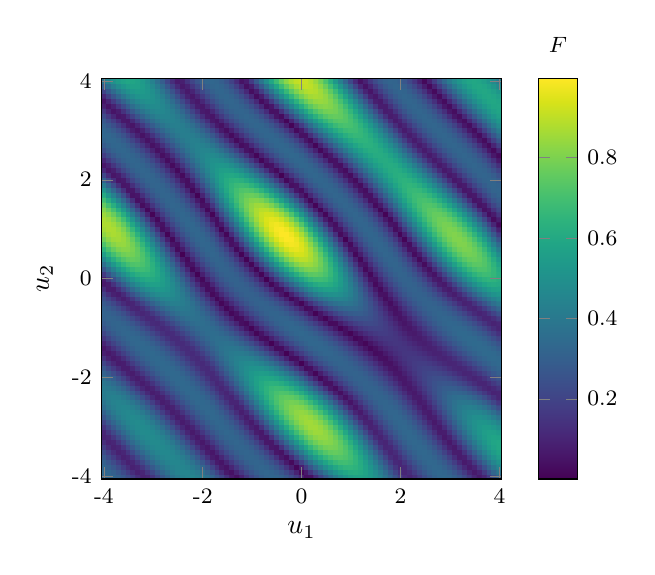
\begin{tikzpicture}[]
\begin{axis}[width=0.55\linewidth, height=0.55\linewidth, xlabel={$u_1$}, ylabel={$u_2$}, colormap/viridis, enlargelimits=false, axis on top, tick label style={font=\footnotesize}, colorbar, xtick={0,20,40,60,80}, xticklabels={-4,-2,0,2,4}, ytick={0,20,40,60,80}, yticklabels={-4,-2,0,2,4}, colorbar style={title=$F$, font=\footnotesize}]
\addplot[matrix plot*, point meta=explicit, mesh/cols=81] table[meta=z] {
x y z
0 0 0.33256
1 0 0.33624
2 0 0.32679
3 0 0.3047
4 0 0.27106
5 0 0.22769
6 0 0.1776
7 0 0.12685
8 0 0.091698
9 0 0.10201
10 0 0.1506
11 0 0.21074
12 0 0.271
13 0 0.32642
14 0 0.37396
15 0 0.41148
16 0 0.4374
17 0 0.45067
18 0 0.45071
19 0 0.43747
20 0 0.41135
21 0 0.37323
22 0 0.32445
23 0 0.26676
24 0 0.20232
25 0 0.13396
26 0 0.06708
27 0 0.039404
28 0 0.092786
29 0 0.15431
30 0 0.21026
31 0 0.25732
32 0 0.29339
33 0 0.317
34 0 0.32713
35 0 0.32326
36 0 0.30534
37 0 0.27382
38 0 0.22959
39 0 0.17402
40 0 0.10885
41 0 0.036437
42 0 0.0428
43 0 0.12327
44 0 0.20415
45 0 0.28256
46 0 0.35592
47 0 0.42184
48 0 0.47814
49 0 0.52299
50 0 0.55493
51 0 0.57293
52 0 0.57641
53 0 0.5653
54 0 0.54005
55 0 0.50157
56 0 0.45131
57 0 0.39122
58 0 0.32378
59 0 0.25235
60 0 0.18206
61 0 0.12367
62 0 0.10244
63 0 0.13206
64 0 0.18268
65 0 0.2335
66 0 0.27684
67 0 0.30923
68 0 0.32876
69 0 0.33441
70 0 0.32582
71 0 0.30326
72 0 0.26763
73 0 0.22052
74 0 0.1647
75 0 0.10636
76 0 0.069586
77 0 0.10141
78 0 0.16948
79 0 0.24406
80 0 0.31708
0 1 0.33624
1 1 0.32666
2 1 0.30439
3 1 0.27054
4 1 0.22693
5 1 0.17664
6 1 0.12582
7 1 0.091222
8 1 0.10284
9 1 0.15223
10 1 0.21274
11 1 0.27317
12 1 0.32863
13 1 0.37611
14 1 0.41346
15 1 0.43912
16 1 0.45202
17 1 0.45163
18 1 0.43787
19 1 0.4112
20 1 0.37251
21 1 0.32317
22 1 0.26498
23 1 0.2002
24 1 0.13182
25 1 0.066114
26 1 0.044158
27 1 0.097592
28 1 0.15852
29 1 0.21383
30 1 0.26004
31 1 0.29504
32 1 0.31731
33 1 0.32585
34 1 0.32012
35 1 0.3001
36 1 0.26625
37 1 0.21953
38 1 0.16132
39 1 0.09351
40 1 0.02003
41 1 0.064459
42 1 0.14763
43 1 0.23115
44 1 0.31206
45 1 0.3877
46 1 0.45563
47 1 0.51362
48 1 0.55979
49 1 0.59263
50 1 0.6111
51 1 0.61461
52 1 0.60307
53 1 0.57692
54 1 0.53709
55 1 0.48503
56 1 0.42267
57 1 0.3525
58 1 0.2777
59 1 0.20289
60 1 0.13695
61 1 0.10222
62 1 0.12255
63 1 0.17227
64 1 0.22474
65 1 0.27031
66 1 0.30494
67 1 0.32653
68 1 0.33393
69 1 0.32675
70 1 0.30522
71 1 0.27019
72 1 0.22324
73 1 0.16708
74 1 0.10768
75 1 0.068701
76 1 0.10019
77 1 0.16969
78 1 0.24593
79 1 0.32072
80 1 0.39012
0 2 0.32669
1 2 0.30431
2 2 0.27028
3 2 0.22645
4 2 0.17592
5 2 0.12498
6 2 0.090817
7 2 0.10365
8 2 0.15388
9 2 0.21487
10 2 0.27564
11 2 0.33133
12 2 0.37895
13 2 0.41634
14 2 0.44194
15 2 0.45469
16 2 0.45404
17 2 0.43996
18 2 0.41288
19 2 0.37375
20 2 0.32395
21 2 0.26532
22 2 0.20021
23 2 0.13179
24 2 0.067107
25 2 0.048307
26 2 0.10102
27 2 0.16145
28 2 0.2163
29 2 0.26193
30 2 0.29614
31 2 0.31738
32 2 0.32463
33 2 0.31735
34 2 0.29552
35 2 0.25964
36 2 0.21068
37 2 0.15009
38 2 0.079999
39 2 0.014024
40 2 0.084576
41 2 0.17042
42 2 0.25662
43 2 0.34013
44 2 0.41823
45 2 0.48837
46 2 0.54831
47 2 0.59609
48 2 0.63017
49 2 0.64946
50 2 0.65334
51 2 0.64172
52 2 0.615
53 2 0.57413
54 2 0.52055
55 2 0.45619
56 2 0.3835
57 2 0.30556
58 2 0.22657
59 2 0.15392
60 2 0.10603
61 2 0.11353
62 2 0.16078
63 2 0.21474
64 2 0.26272
65 2 0.29991
66 2 0.32392
67 2 0.3335
68 2 0.32817
69 2 0.30809
70 2 0.27409
71 2 0.22769
72 2 0.17147
73 2 0.11102
74 2 0.068157
75 2 0.0966
76 2 0.1668
77 2 0.24447
78 2 0.32094
79 2 0.39217
80 2 0.45525
0 3 0.30451
1 3 0.27037
2 3 0.22637
3 3 0.17562
4 3 0.12449
5 3 0.090569
6 3 0.10434
7 3 0.15533
8 3 0.21688
9 3 0.2781
10 3 0.33417
11 3 0.3821
12 3 0.41973
13 3 0.44547
14 3 0.45828
15 3 0.45759
16 3 0.44336
17 3 0.41606
18 3 0.37663
19 3 0.32648
20 3 0.2675
21 3 0.2021
22 3 0.13361
23 3 0.069675
24 3 0.051836
25 3 0.10322
26 3 0.16324
27 3 0.21784
28 3 0.26314
29 3 0.29686
30 3 0.3174
31 3 0.32371
32 3 0.31523
33 3 0.29196
34 3 0.25439
35 3 0.20352
36 3 0.14091
37 3 0.069122
38 3 0.02336
39 3 0.10246
40 3 0.19086
41 3 0.27972
42 3 0.36589
43 3 0.44655
44 3 0.5191
45 3 0.5812
46 3 0.63088
47 3 0.66652
48 3 0.68698
49 3 0.69162
50 3 0.68029
51 3 0.6534
52 3 0.61187
53 3 0.55712
54 3 0.49109
55 3 0.41618
56 3 0.3354
57 3 0.25264
58 3 0.17413
59 3 0.11445
60 3 0.10604
61 3 0.14847
62 3 0.20349
63 3 0.25397
64 3 0.29397
65 3 0.32077
66 3 0.33293
67 3 0.32988
68 3 0.31172
69 3 0.27921
70 3 0.23379
71 3 0.17792
72 3 0.11661
73 3 0.068725
74 3 0.090772
75 3 0.1607
76 3 0.23944
77 3 0.31742
78 3 0.39041
79 3 0.45541
80 3 0.51001
0 4 0.27089
1 4 0.22679
2 4 0.17586
3 4 0.12451
4 4 0.090558
5 4 0.10481
6 4 0.1564
7 4 0.21849
8 4 0.28024
9 4 0.33681
10 4 0.38521
11 4 0.42324
12 4 0.44933
13 4 0.46239
14 4 0.46186
15 4 0.44769
16 4 0.42035
17 4 0.38079
18 4 0.33043
19 4 0.27121
20 4 0.20556
21 4 0.13699
22 4 0.073473
23 4 0.054846
24 4 0.10436
25 4 0.16401
26 4 0.21856
27 4 0.2638
28 4 0.29733
29 4 0.31752
30 4 0.32326
31 4 0.31398
32 4 0.28967
33 4 0.25081
34 4 0.19845
35 4 0.13427
36 4 0.061629
37 4 0.035132
38 4 0.1175
39 4 0.20825
40 4 0.29967
41 4 0.38846
42 4 0.47173
43 4 0.5468
44 4 0.61127
45 4 0.66309
46 4 0.7006
47 4 0.72259
48 4 0.72836
49 4 0.71775
50 4 0.69112
51 4 0.64935
52 4 0.59385
53 4 0.52655
54 4 0.44982
55 4 0.36658
56 4 0.28049
57 4 0.19696
58 4 0.12733
59 4 0.10143
60 4 0.1357
61 4 0.19102
62 4 0.24398
63 4 0.28699
64 4 0.31687
65 4 0.33199
66 4 0.33165
67 4 0.31587
68 4 0.28532
69 4 0.24138
70 4 0.18631
71 4 0.12456
72 4 0.071404
73 4 0.08319
74 4 0.15143
75 4 0.23076
76 4 0.30997
77 4 0.38455
78 4 0.4514
79 4 0.50803
80 4 0.55244
0 5 0.22777
1 5 0.17673
2 5 0.12516
3 5 0.090857
4 5 0.105
5 5 0.15689
6 5 0.21946
7 5 0.28176
8 5 0.33891
9 5 0.38789
10 5 0.42648
11 5 0.45308
12 5 0.46658
13 5 0.46642
14 5 0.45252
15 5 0.42534
16 5 0.38583
17 5 0.33543
18 5 0.27608
19 5 0.21028
20 5 0.14162
21 5 0.078203
22 5 0.057484
23 5 0.10458
24 5 0.16388
25 5 0.21853
26 5 0.26395
27 5 0.29761
28 5 0.3178
29 5 0.32336
30 5 0.3137
31 5 0.28878
32 5 0.24909
33 5 0.19572
34 5 0.1305
35 5 0.058016
36 5 0.045219
37 5 0.12921
38 5 0.22199
39 5 0.31576
40 5 0.40707
41 5 0.49292
42 5 0.57055
43 5 0.63752
44 5 0.69168
45 5 0.73131
46 5 0.75515
47 5 0.76245
48 5 0.75297
49 5 0.72704
50 5 0.6855
51 5 0.62974
52 5 0.56164
53 5 0.48354
54 5 0.3983
55 5 0.3094
56 5 0.22163
57 5 0.14395
58 5 0.10098
59 5 0.12304
60 5 0.17744
61 5 0.2327
62 5 0.27883
63 5 0.31202
64 5 0.33041
65 5 0.33316
66 5 0.32019
67 5 0.29209
68 5 0.25012
69 5 0.1964
70 5 0.13478
71 5 0.077074
72 5 0.074839
73 5 0.13927
74 5 0.21851
75 5 0.29856
76 5 0.37446
77 5 0.44299
78 5 0.50158
79 5 0.54812
80 5 0.58104
0 6 0.1783
1 6 0.12651
2 6 0.091534
3 6 0.10484
4 6 0.15667
5 6 0.21959
6 6 0.28241
7 6 0.34017
8 6 0.3898
9 6 0.42906
10 6 0.45632
11 6 0.47044
12 6 0.47083
13 6 0.4574
14 6 0.43058
15 6 0.39132
16 6 0.34106
17 6 0.28174
18 6 0.2159
19 6 0.14717
20 6 0.083608
21 6 0.059908
22 6 0.10402
23 6 0.16293
24 6 0.21782
25 6 0.26364
26 6 0.29771
27 6 0.31823
28 6 0.324
29 6 0.31439
30 6 0.28933
31 6 0.24931
32 6 0.19545
33 6 0.12977
34 6 0.0583
35 6 0.052895
36 6 0.13729
37 6 0.23165
38 6 0.32746
39 6 0.42107
40 6 0.50936
41 6 0.58952
42 6 0.65901
43 6 0.71564
44 6 0.7576
45 6 0.78358
46 6 0.79275
47 6 0.78481
48 6 0.76003
49 6 0.71921
50 6 0.6637
51 6 0.59532
52 6 0.51638
53 6 0.42967
54 6 0.33853
55 6 0.24729
56 6 0.16322
57 6 0.10538
58 6 0.11132
59 6 0.16296
60 6 0.22016
61 6 0.26941
62 6 0.30605
63 6 0.32795
64 6 0.33411
65 6 0.32434
66 6 0.29912
67 6 0.25962
68 6 0.20778
69 6 0.14697
70 6 0.0861
71 6 0.067425
72 6 0.12471
73 6 0.20297
74 6 0.28334
75 6 0.36021
76 6 0.43016
77 6 0.49052
78 6 0.53911
79 6 0.57427
80 6 0.5948
0 7 0.1286
1 7 0.09265
2 7 0.10435
3 7 0.15564
4 7 0.21871
5 7 0.28195
6 7 0.3403
7 7 0.39062
8 7 0.43063
9 7 0.45865
10 7 0.47354
11 7 0.47465
12 7 0.46188
13 7 0.43563
14 7 0.39682
15 7 0.3469
16 7 0.28779
17 7 0.22203
18 7 0.1533
19 7 0.089443
20 7 0.062262
21 7 0.10284
22 7 0.16127
23 7 0.21648
24 7 0.26287
25 7 0.29759
26 7 0.31875
27 7 0.32511
28 7 0.31597
29 7 0.29124
30 7 0.2514
31 7 0.19758
32 7 0.13203
33 7 0.062019
34 7 0.05819
35 7 0.14163
36 7 0.23698
37 7 0.33441
38 7 0.42998
39 7 0.52048
40 7 0.60302
41 7 0.67499
42 7 0.73411
43 7 0.77854
44 7 0.80686
45 7 0.81818
46 7 0.81214
47 7 0.78895
48 7 0.74934
49 7 0.69459
50 7 0.62648
51 7 0.54728
52 7 0.4597
53 7 0.36694
54 7 0.27302
55 7 0.18399
56 7 0.11427
57 7 0.10157
58 7 0.14789
59 7 0.20649
60 7 0.25873
61 7 0.29886
62 7 0.3244
63 7 0.3342
64 7 0.32793
65 7 0.30598
66 7 0.2694
67 7 0.21997
68 7 0.16066
69 7 0.098205
70 7 0.063427
71 7 0.10861
72 7 0.1846
73 7 0.26467
74 7 0.34204
75 7 0.41304
76 7 0.47489
77 7 0.52535
78 7 0.56266
79 7 0.58555
80 7 0.59328
0 8 0.094258
1 8 0.10356
2 8 0.15376
3 8 0.21671
4 8 0.28025
5 8 0.33911
6 8 0.39009
7 8 0.43087
8 8 0.45973
9 8 0.47548
10 8 0.47745
11 8 0.4655
12 8 0.44001
13 8 0.40187
14 8 0.35248
15 8 0.29378
16 8 0.22828
17 8 0.15965
18 8 0.095464
19 8 0.064653
20 8 0.10119
21 8 0.159
22 8 0.21455
23 8 0.26163
24 8 0.29719
25 8 0.31927
26 8 0.32654
27 8 0.31827
28 8 0.29432
29 8 0.25514
30 8 0.20191
31 8 0.13703
32 8 0.068534
33 8 0.061557
34 8 0.14235
35 8 0.23795
36 8 0.33646
37 8 0.43356
38 8 0.52593
39 8 0.61059
40 8 0.68486
41 8 0.74641
42 8 0.79331
43 8 0.82409
44 8 0.83778
45 8 0.83395
46 8 0.81272
47 8 0.77476
48 8 0.72129
49 8 0.65402
50 8 0.57515
51 8 0.48732
52 8 0.39362
53 8 0.2978
54 8 0.20508
55 8 0.12642
56 8 0.094845
57 8 0.13266
58 8 0.19188
59 8 0.24688
60 8 0.29042
61 8 0.31964
62 8 0.33319
63 8 0.33064
64 8 0.31225
65 8 0.27897
66 8 0.23242
67 8 0.17523
68 8 0.11266
69 8 0.065227
70 8 0.092252
71 8 0.1641
72 8 0.24306
73 8 0.32036
74 8 0.39196
75 8 0.45495
76 8 0.50699
77 8 0.54625
78 8 0.57139
79 8 0.58158
80 8 0.57654
0 9 0.10257
1 9 0.15107
2 9 0.21358
3 9 0.27721
4 9 0.33645
5 9 0.38802
6 9 0.42953
7 9 0.45925
8 9 0.47592
9 9 0.47886
10 9 0.46788
11 9 0.44331
12 9 0.40602
13 9 0.35737
14 9 0.29927
15 9 0.23424
16 9 0.16586
17 9 0.10141
18 9 0.067128
19 9 0.099259
20 9 0.15625
21 9 0.21212
22 9 0.25994
23 9 0.29648
24 9 0.31967
25 9 0.32812
26 9 0.32105
27 9 0.29828
28 9 0.26024
29 9 0.2081
30 9 0.14438
31 9 0.077271
32 9 0.063808
33 9 0.13979
34 9 0.23474
35 9 0.33368
36 9 0.43178
37 9 0.52556
38 9 0.61197
39 9 0.68827
40 9 0.75206
41 9 0.80136
42 9 0.83461
43 9 0.85078
44 9 0.84936
45 9 0.83039
46 9 0.79448
47 9 0.74275
48 9 0.67686
49 9 0.59891
50 9 0.51147
51 9 0.41753
52 9 0.3206
53 9 0.22533
54 9 0.14026
55 9 0.091811
56 9 0.11776
57 9 0.17666
58 9 0.23409
59 9 0.28084
60 9 0.31363
61 9 0.33093
62 9 0.33219
63 9 0.31755
64 9 0.28785
65 9 0.24457
66 9 0.19005
67 9 0.12854
68 9 0.073346
69 9 0.077641
70 9 0.14235
71 9 0.21921
72 9 0.2958
73 9 0.36746
74 9 0.43112
75 9 0.48436
76 9 0.52528
77 9 0.55245
78 9 0.56498
79 9 0.56251
80 9 0.54519
0 10 0.14765
1 10 0.20936
2 10 0.27283
3 10 0.33228
4 10 0.3843
5 10 0.42647
6 10 0.45699
7 10 0.47461
8 10 0.47856
9 10 0.46863
10 10 0.44512
11 10 0.40884
12 10 0.36113
13 10 0.30385
14 10 0.23947
15 10 0.17154
16 10 0.10699
17 10 0.06966
18 10 0.09723
19 10 0.15321
20 10 0.20929
21 10 0.25784
22 10 0.29541
23 10 0.31983
24 10 0.32967
25 10 0.32408
26 10 0.30283
27 10 0.26632
28 10 0.21572
29 10 0.15357
30 10 0.087765
31 10 0.066017
32 10 0.13454
33 10 0.22777
34 10 0.32639
35 10 0.42487
36 10 0.51951
37 10 0.6072
38 10 0.68513
39 10 0.75086
40 10 0.80234
41 10 0.83795
42 10 0.8566
43 10 0.85769
44 10 0.8412
45 10 0.80764
46 10 0.75805
47 10 0.69401
48 10 0.61755
49 10 0.53113
50 10 0.43763
51 10 0.3404
52 10 0.24362
53 10 0.15418
54 10 0.092259
55 10 0.10373
56 10 0.16124
57 10 0.22068
58 10 0.27035
59 10 0.30649
60 10 0.3274
61 10 0.33242
62 10 0.32159
63 10 0.29563
64 10 0.25589
65 10 0.20448
66 10 0.14492
67 10 0.08617
68 10 0.067621
69 10 0.12052
70 10 0.19398
71 10 0.2691
72 10 0.34022
73 10 0.40402
74 10 0.458
75 10 0.50018
76 10 0.52909
77 10 0.54374
78 10 0.54369
79 10 0.52904
80 10 0.50038
0 11 0.20416
1 11 0.26719
2 11 0.32662
3 11 0.37892
4 11 0.42161
5 11 0.45285
6 11 0.47135
7 11 0.47631
8 11 0.46749
9 11 0.44512
10 11 0.40999
11 11 0.36338
12 11 0.30711
13 11 0.2436
14 11 0.17632
15 11 0.11192
16 11 0.072147
17 11 0.095292
18 11 0.15005
19 11 0.20623
20 11 0.25542
21 11 0.294
22 11 0.3197
23 11 0.33103
24 11 0.3271
25 11 0.30763
26 11 0.27298
27 11 0.22429
28 11 0.16406
29 11 0.099592
30 11 0.069304
31 11 0.12742
32 11 0.21763
33 11 0.3151
34 11 0.41325
35 11 0.50814
36 11 0.59654
37 11 0.67562
38 11 0.74287
39 11 0.7962
40 11 0.83395
41 11 0.85495
42 11 0.85854
43 11 0.84461
44 11 0.8136
45 11 0.76646
46 11 0.70468
47 11 0.63019
48 11 0.54537
49 11 0.45299
50 11 0.35621
51 11 0.25888
52 11 0.16675
53 11 0.095048
54 11 0.090983
55 11 0.14608
56 11 0.20711
57 11 0.25931
58 11 0.29845
59 11 0.3227
60 11 0.3313
61 11 0.3242
62 11 0.302
63 11 0.26594
64 11 0.21792
65 11 0.16097
66 11 0.10148
67 11 0.065048
68 11 0.10007
69 11 0.16834
70 11 0.24113
71 11 0.31106
72 11 0.37443
73 11 0.42862
74 11 0.4716
75 11 0.50183
76 11 0.51828
77 11 0.52043
78 11 0.50829
79 11 0.48239
80 11 0.44378
0 12 0.26045
1 12 0.3196
2 12 0.37195
3 12 0.41497
4 12 0.44679
5 12 0.46606
6 12 0.47198
7 12 0.46425
8 12 0.44307
9 12 0.40916
10 12 0.36378
11 12 0.30868
12 12 0.24624
13 12 0.17985
14 12 0.11588
15 12 0.074429
16 12 0.093614
17 12 0.14702
18 12 0.20312
19 12 0.25282
20 12 0.2923
21 12 0.31924
22 12 0.33209
23 12 0.32991
24 12 0.31239
25 12 0.27983
26 12 0.23332
27 12 0.1753
28 12 0.11231
29 12 0.074488
30 12 0.11941
31 12 0.20508
32 12 0.30049
33 12 0.39756
34 12 0.49201
35 12 0.5805
36 12 0.66015
37 12 0.72842
38 12 0.78318
39 12 0.82272
40 12 0.84582
41 12 0.85177
42 12 0.84037
43 12 0.81198
44 12 0.76748
45 12 0.70826
46 12 0.63615
47 12 0.55344
48 12 0.46277
49 12 0.36716
50 12 0.27017
51 12 0.17674
52 12 0.098522
53 12 0.079746
54 12 0.13171
55 12 0.19393
56 12 0.2482
57 12 0.28989
58 12 0.31708
59 12 0.32894
60 12 0.32533
61 12 0.30678
62 12 0.27439
63 12 0.22991
64 12 0.17597
65 12 0.11747
66 12 0.070333
67 12 0.082899
68 12 0.14335
69 12 0.21285
70 12 0.28089
71 12 0.34322
72 12 0.39706
73 12 0.44032
74 12 0.47141
75 12 0.48926
76 12 0.49328
77 12 0.48341
78 12 0.46011
79 12 0.42434
80 12 0.37759
0 13 0.31142
1 13 0.36357
2 13 0.4067
3 13 0.43889
4 13 0.45879
5 13 0.46555
6 13 0.45883
7 13 0.43881
8 13 0.40617
9 13 0.36209
10 13 0.3083
11 13 0.2471
12 13 0.18182
13 13 0.11861
14 13 0.076314
15 13 0.092336
16 13 0.14436
17 13 0.20019
18 13 0.25021
19 13 0.29043
20 13 0.31848
21 13 0.33278
22 13 0.33236
23 13 0.31684
24 13 0.2865
25 13 0.24237
26 13 0.18674
27 13 0.12546
28 13 0.08182
29 13 0.11165
30 13 0.19099
31 13 0.28338
32 13 0.3786
33 13 0.4719
34 13 0.55981
35 13 0.6394
36 13 0.7081
37 13 0.76376
38 13 0.80465
39 13 0.8295
40 13 0.83753
41 13 0.8285
42 13 0.80269
43 13 0.76089
44 13 0.70441
45 13 0.63498
46 13 0.55478
47 13 0.46633
48 13 0.37252
49 13 0.27667
50 13 0.18311
51 13 0.10101
52 13 0.06989
53 13 0.11867
54 13 0.1818
55 13 0.23762
56 13 0.28131
57 13 0.31092
58 13 0.32558
59 13 0.32511
60 13 0.30993
61 13 0.28106
62 13 0.24009
63 13 0.18937
64 13 0.13285
65 13 0.080839
66 13 0.071178
67 13 0.12015
68 13 0.1852
69 13 0.25065
70 13 0.31134
71 13 0.36426
72 13 0.40725
73 13 0.43868
74 13 0.45745
75 13 0.46293
76 13 0.45501
77 13 0.43406
78 13 0.40099
79 13 0.35719
80 13 0.30462
0 14 0.35403
1 14 0.397
2 14 0.42933
3 14 0.44965
4 14 0.45708
5 14 0.45126
6 14 0.43232
7 14 0.40091
8 14 0.35817
9 14 0.30576
10 14 0.24594
11 14 0.18197
12 14 0.11987
13 14 0.077623
14 14 0.091567
15 14 0.14229
16 14 0.19769
17 14 0.2478
18 14 0.28854
19 14 0.31752
20 14 0.33312
21 14 0.33434
22 14 0.3208
23 14 0.2927
24 14 0.25103
25 14 0.19793
26 14 0.13856
27 14 0.090985
28 14 0.10527
29 14 0.17632
30 14 0.26467
31 14 0.35726
32 14 0.4487
33 14 0.53535
34 14 0.61421
35 14 0.68272
36 14 0.7387
37 14 0.78041
38 14 0.80653
39 14 0.81628
40 14 0.80934
41 14 0.78593
42 14 0.74677
43 14 0.69308
44 14 0.6265
45 14 0.5491
46 14 0.46328
47 14 0.37181
48 14 0.27777
49 14 0.18506
50 14 0.10112
51 14 0.060969
52 14 0.10758
53 14 0.17141
54 14 0.22822
55 14 0.27328
56 14 0.30469
57 14 0.32159
58 14 0.32375
59 14 0.31156
60 14 0.28591
61 14 0.24827
62 14 0.20079
63 14 0.14677
64 14 0.093391
65 14 0.066493
66 14 0.099883
67 14 0.15911
68 14 0.22128
69 14 0.27973
70 14 0.33117
71 14 0.37334
72 14 0.4046
73 14 0.42379
74 14 0.43028
75 14 0.42389
76 14 0.40497
77 14 0.37435
78 14 0.33337
79 14 0.28393
80 14 0.22867
0 15 0.38617
1 15 0.41839
2 15 0.43888
3 15 0.44676
4 15 0.44166
5 15 0.42368
6 15 0.39342
7 15 0.35199
8 15 0.30098
9 15 0.24263
10 15 0.18014
11 15 0.11948
12 15 0.078231
13 15 0.091394
14 15 0.14104
15 15 0.19586
16 15 0.24581
17 15 0.28683
18 15 0.31648
19 15 0.33316
20 15 0.33586
21 15 0.32416
22 15 0.29823
23 15 0.259
24 15 0.20847
25 15 0.15119
26 15 0.10133
27 15 0.10119
28 15 0.162
29 15 0.24526
30 15 0.33449
31 15 0.4234
32 15 0.50812
33 15 0.5856
34 15 0.65326
35 15 0.70894
36 15 0.75087
37 15 0.77775
38 15 0.78874
39 15 0.7835
40 15 0.76221
41 15 0.7255
42 15 0.67452
43 15 0.61082
44 15 0.53638
45 15 0.45348
46 15 0.36474
47 15 0.27308
48 15 0.18203
49 15 0.097823
50 15 0.052428
51 15 0.099159
52 15 0.16351
53 15 0.2207
54 15 0.26642
55 15 0.29894
56 15 0.31742
57 15 0.32163
58 15 0.31188
59 15 0.28903
60 15 0.25442
61 15 0.21001
62 15 0.15867
63 15 0.10579
64 15 0.068266
65 15 0.083638
66 15 0.13536
67 15 0.19358
68 15 0.2493
69 15 0.29875
70 15 0.33959
71 15 0.37014
72 15 0.38925
73 15 0.39625
74 15 0.39097
75 15 0.3737
76 15 0.34524
77 15 0.30688
78 15 0.26049
79 15 0.20878
80 15 0.15611
0 16 0.40639
1 16 0.42679
2 16 0.43489
3 16 0.43029
4 16 0.41307
5 16 0.38383
6 16 0.34361
7 16 0.29399
8 16 0.23715
9 16 0.17627
10 16 0.11738
11 16 0.078108
12 16 0.091899
13 16 0.14079
14 16 0.19491
15 16 0.24448
16 16 0.28548
17 16 0.31553
18 16 0.33301
19 16 0.33694
20 16 0.32687
21 16 0.30296
22 16 0.26606
23 16 0.21805
24 16 0.16296
25 16 0.11212
26 16 0.099879
27 16 0.14892
28 16 0.22606
29 16 0.31122
30 16 0.39697
31 16 0.47915
32 16 0.55463
33 16 0.62081
34 16 0.67555
35 16 0.7171
36 16 0.74415
37 16 0.75586
38 16 0.75186
39 16 0.73229
40 16 0.69773
41 16 0.64926
42 16 0.58836
43 16 0.5169
44 16 0.43706
45 16 0.35134
46 16 0.26248
47 16 0.17372
48 16 0.090455
49 16 0.044089
50 16 0.094245
51 16 0.15881
52 16 0.2157
53 16 0.26135
54 16 0.29424
55 16 0.31357
56 16 0.31914
57 16 0.31123
58 16 0.29063
59 16 0.25861
60 16 0.21697
61 16 0.16826
62 16 0.11677
63 16 0.073881
64 16 0.072142
65 16 0.11459
66 16 0.16824
67 16 0.2208
68 16 0.26785
69 16 0.30691
70 16 0.33628
71 16 0.35482
72 16 0.36187
73 16 0.35723
74 16 0.34121
75 16 0.31457
76 16 0.27859
77 16 0.23518
78 16 0.18718
79 16 0.13953
80 16 0.10291
0 17 0.41377
1 17 0.42181
2 17 0.41746
3 17 0.40079
4 17 0.37237
5 17 0.33323
6 17 0.28491
7 17 0.22957
8 17 0.17039
9 17 0.11359
10 17 0.077353
11 17 0.093179
12 17 0.14168
13 17 0.19502
14 17 0.24398
15 17 0.28469
16 17 0.31482
17 17 0.33281
18 17 0.33767
19 17 0.32896
20 17 0.30682
21 17 0.27206
22 17 0.22644
23 17 0.17356
24 17 0.1227
25 17 0.10121
26 17 0.13777
27 17 0.20785
28 17 0.28833
29 17 0.3704
30 17 0.44949
31 17 0.5224
32 17 0.58652
33 17 0.63972
34 17 0.68028
35 17 0.7069
36 17 0.71876
37 17 0.71548
38 17 0.69716
39 17 0.66437
40 17 0.61811
41 17 0.5598
42 17 0.49122
43 17 0.41446
44 17 0.3319
45 17 0.24613
46 17 0.16013
47 17 0.078721
48 17 0.037054
49 17 0.09373
50 17 0.1579
51 17 0.21375
52 17 0.25858
53 17 0.29107
54 17 0.31052
55 17 0.31673
56 17 0.30999
57 17 0.29103
58 17 0.26106
59 17 0.22176
60 17 0.17543
61 17 0.12567
62 17 0.080598
63 17 0.065334
64 17 0.097138
65 17 0.14574
66 17 0.19485
67 17 0.23919
68 17 0.27611
69 17 0.30391
70 17 0.32144
71 17 0.32809
72 17 0.32367
73 17 0.30849
74 17 0.28333
75 17 0.2495
76 17 0.20902
77 17 0.16505
78 17 0.12349
79 17 0.097095
80 17 0.103
0 18 0.40794
1 18 0.40356
2 18 0.38719
3 18 0.35938
4 18 0.32113
5 18 0.27399
6 18 0.22007
7 18 0.16265
8 18 0.10826
9 18 0.076212
10 18 0.09534
11 18 0.14378
12 18 0.19628
13 18 0.24444
14 18 0.2846
15 18 0.31452
16 18 0.33269
17 18 0.33815
18 18 0.33048
19 18 0.30983
20 18 0.27696
21 18 0.23352
22 18 0.18279
23 18 0.13254
24 18 0.10456
25 18 0.12903
26 18 0.1913
27 18 0.26661
28 18 0.34456
29 18 0.42013
30 18 0.48998
31 18 0.55151
32 18 0.60262
33 18 0.64161
34 18 0.66723
35 18 0.67867
36 18 0.67555
37 18 0.65798
38 18 0.6265
39 18 0.58207
40 18 0.52605
41 18 0.46015
42 18 0.38637
43 18 0.30698
44 18 0.22444
45 18 0.14151
46 18 0.062675
47 18 0.034917
48 18 0.098249
49 18 0.16112
50 18 0.21519
51 18 0.25847
52 18 0.28983
53 18 0.30866
54 18 0.31479
55 18 0.30851
56 18 0.29053
57 18 0.26202
58 18 0.22454
59 18 0.18023
60 18 0.1322
61 18 0.086599
62 18 0.062113
63 18 0.083004
64 18 0.12629
65 18 0.17184
66 18 0.21331
67 18 0.24785
68 18 0.27376
69 18 0.28994
70 18 0.2958
71 18 0.29122
72 18 0.27652
73 18 0.25254
74 18 0.22069
75 18 0.1832
76 18 0.14383
77 18 0.11003
78 18 0.096188
79 18 0.1129
80 18 0.14937
0 19 0.38904
1 19 0.3727
2 19 0.34524
3 19 0.30768
4 19 0.26153
5 19 0.20894
6 19 0.15329
7 19 0.10167
8 19 0.075067
9 19 0.098483
10 19 0.14711
11 19 0.19873
12 19 0.24593
13 19 0.28529
14 19 0.31471
15 19 0.33274
16 19 0.33847
17 19 0.33152
18 19 0.31202
19 19 0.28072
20 19 0.23922
21 19 0.1905
22 19 0.14125
23 19 0.10909
24 19 0.12282
25 19 0.1769
26 19 0.24669
27 19 0.32022
28 19 0.39193
29 19 0.45835
30 19 0.51686
31 19 0.5654
32 19 0.60231
33 19 0.62639
34 19 0.63685
35 19 0.63336
36 19 0.61602
37 19 0.58536
38 19 0.54232
39 19 0.48821
40 19 0.4247
41 19 0.3537
42 19 0.27738
43 19 0.19808
44 19 0.1184
45 19 0.04276
46 19 0.041895
47 19 0.10786
48 19 0.16847
49 19 0.22007
50 19 0.26114
51 19 0.29071
52 19 0.30823
53 19 0.31359
54 19 0.30709
55 19 0.28944
56 19 0.26175
57 19 0.22555
58 19 0.1828
59 19 0.13627
60 19 0.090908
61 19 0.06075
62 19 0.071808
63 19 0.1099
64 19 0.15198
65 19 0.19055
66 19 0.22259
67 19 0.24641
68 19 0.26098
69 19 0.26576
70 19 0.26069
71 19 0.24618
72 19 0.22316
73 19 0.19323
74 19 0.159
75 19 0.12526
76 19 0.10145
77 19 0.1012
78 19 0.12627
79 19 0.16426
80 19 0.20533
0 20 0.35777
1 20 0.3304
2 20 0.29328
3 20 0.24792
4 20 0.19652
5 20 0.14264
6 20 0.09421
7 20 0.074391
8 20 0.10267
9 20 0.1516
10 20 0.20231
11 20 0.24841
12 20 0.28679
13 20 0.31545
14 20 0.33304
15 20 0.33871
16 20 0.33212
17 20 0.31343
18 20 0.28339
19 20 0.24351
20 20 0.19662
21 20 0.14858
22 20 0.11398
23 20 0.11895
24 20 0.16495
25 20 0.22907
26 20 0.29801
27 20 0.36565
28 20 0.42837
29 20 0.48353
30 20 0.52911
31 20 0.56351
32 20 0.58557
33 20 0.59457
34 20 0.59019
35 20 0.57256
36 20 0.54222
37 20 0.50011
38 20 0.44751
39 20 0.38602
40 20 0.31752
41 20 0.24408
42 20 0.16794
43 20 0.091546
44 20 0.020333
45 20 0.057378
46 20 0.12199
47 20 0.17958
48 20 0.22817
49 20 0.26649
50 20 0.29369
51 20 0.3093
52 20 0.31326
53 20 0.30591
54 20 0.28795
55 20 0.26049
56 20 0.22498
57 20 0.1833
58 20 0.13795
59 20 0.093072
60 20 0.059624
61 20 0.062861
62 20 0.096368
63 20 0.13529
64 20 0.17109
65 20 0.20062
66 20 0.22225
67 20 0.23503
68 20 0.23851
69 20 0.23272
70 20 0.21819
71 20 0.19602
72 20 0.1681
73 20 0.13774
74 20 0.11118
75 20 0.099416
76 20 0.11148
77 20 0.14206
78 20 0.18049
79 20 0.21991
80 20 0.2564
0 21 0.31532
1 21 0.27838
2 21 0.23358
3 21 0.1832
4 21 0.13106
5 21 0.086354
6 21 0.074651
7 21 0.10786
8 21 0.15711
9 21 0.20689
10 21 0.2518
11 21 0.28901
12 21 0.31669
13 21 0.33357
14 21 0.33888
15 21 0.33233
16 21 0.3141
17 21 0.28497
18 21 0.24642
19 21 0.20111
20 21 0.15437
21 21 0.1186
22 21 0.11698
23 21 0.15552
24 21 0.21407
25 21 0.27841
26 21 0.3419
27 21 0.40076
28 21 0.45235
29 21 0.49469
30 21 0.52623
31 21 0.54588
32 21 0.55297
33 21 0.54724
34 21 0.52886
35 21 0.49837
36 21 0.45673
37 21 0.40519
38 21 0.34535
39 21 0.27902
40 21 0.2082
41 21 0.13505
42 21 0.061873
43 21 0.012986
44 21 0.078172
45 21 0.13969
46 21 0.19379
47 21 0.23897
48 21 0.27413
49 21 0.2985
50 21 0.31171
51 21 0.31375
52 21 0.30498
53 21 0.28615
54 21 0.25835
55 21 0.22299
56 21 0.18188
57 21 0.13733
58 21 0.092913
59 21 0.057595
60 21 0.05537
61 21 0.085419
62 21 0.12171
63 21 0.15497
64 21 0.18208
65 21 0.2015
66 21 0.21239
67 21 0.21443
68 21 0.20776
69 21 0.19308
70 21 0.17174
71 21 0.14612
72 21 0.12057
73 21 0.10302
74 21 0.10384
75 21 0.12525
76 21 0.15906
77 21 0.19725
78 21 0.2349
79 21 0.26896
80 21 0.29733
0 22 0.26342
1 22 0.21895
2 22 0.16939
3 22 0.11896
4 22 0.078667
5 22 0.076184
6 22 0.11396
7 22 0.16343
8 22 0.21226
9 22 0.2559
10 22 0.29182
11 22 0.31833
12 22 0.33427
13 22 0.33895
14 22 0.33212
15 22 0.31403
16 22 0.28547
17 22 0.24792
18 22 0.20397
19 22 0.15851
20 22 0.12247
21 22 0.11634
22 22 0.14854
23 22 0.20187
24 22 0.26174
25 22 0.32112
26 22 0.37608
27 22 0.42399
28 22 0.4629
29 22 0.49133
30 22 0.50827
31 22 0.5131
32 22 0.50563
33 22 0.48607
34 22 0.45501
35 22 0.4134
36 22 0.36252
37 22 0.30392
38 22 0.2394
39 22 0.1709
40 22 0.1005
41 22 0.030432
42 22 0.038183
43 22 0.10193
44 22 0.15983
45 22 0.21021
46 22 0.25176
47 22 0.28347
48 22 0.30469
49 22 0.3151
50 22 0.31477
51 22 0.30413
52 22 0.28394
53 22 0.2553
54 22 0.21961
55 22 0.17862
56 22 0.13447
57 22 0.090371
58 22 0.053987
59 22 0.048698
60 22 0.076876
61 22 0.11118
62 22 0.1422
63 22 0.16702
64 22 0.18425
65 22 0.1932
66 22 0.19368
67 22 0.18602
68 22 0.17111
69 22 0.15068
70 22 0.12783
71 22 0.10825
72 22 0.10097
73 22 0.11285
74 22 0.14056
75 22 0.17614
76 22 0.21373
77 22 0.24962
78 22 0.28134
79 22 0.30707
80 22 0.32548
0 23 0.20444
1 23 0.1555
2 23 0.10677
3 23 0.071742
4 23 0.079091
5 23 0.12074
6 23 0.1703
7 23 0.21816
8 23 0.26048
9 23 0.29501
10 23 0.3202
11 23 0.33501
12 23 0.3388
13 23 0.33142
14 23 0.31316
15 23 0.28487
16 23 0.24802
17 23 0.20516
18 23 0.16096
19 23 0.12531
20 23 0.11651
21 23 0.1438
22 23 0.19251
23 23 0.24822
24 23 0.30364
25 23 0.35477
26 23 0.39898
27 23 0.43436
28 23 0.45953
29 23 0.47353
30 23 0.47584
31 23 0.46631
32 23 0.44523
33 23 0.41321
34 23 0.37124
35 23 0.32062
36 23 0.2629
37 23 0.19983
38 23 0.13333
39 23 0.065422
40 23 0.0027831
41 23 0.066746
42 23 0.12707
43 23 0.18128
44 23 0.22788
45 23 0.26568
46 23 0.29377
47 23 0.3116
48 23 0.31893
49 23 0.31591
50 23 0.30302
51 23 0.28106
52 23 0.25117
53 23 0.21474
54 23 0.17345
55 23 0.12937
56 23 0.085388
57 23 0.048422
58 23 0.042645
59 23 0.070836
60 23 0.1038
61 23 0.13285
62 23 0.15548
63 23 0.17054
64 23 0.17749
65 23 0.17631
66 23 0.16752
67 23 0.15231
68 23 0.13288
69 23 0.11332
70 23 0.10072
71 23 0.10365
72 23 0.12406
73 23 0.15583
74 23 0.19235
75 23 0.22919
76 23 0.26342
77 23 0.29293
78 23 0.31615
79 23 0.33191
80 23 0.33941
0 24 0.14189
1 24 0.094848
2 24 0.066129
3 24 0.083216
4 24 0.12791
5 24 0.17742
6 24 0.22429
7 24 0.26526
8 24 0.29833
9 24 0.32209
10 24 0.33559
11 24 0.33829
12 24 0.33011
13 24 0.31142
14 24 0.28309
15 24 0.24666
16 24 0.20467
17 24 0.16166
18 24 0.12695
19 24 0.1171
20 24 0.14105
21 24 0.18596
22 24 0.23795
23 24 0.28968
24 24 0.33712
25 24 0.37769
26 24 0.40954
27 24 0.43137
28 24 0.4423
29 24 0.44189
30 24 0.43007
31 24 0.40717
32 24 0.37389
33 24 0.33123
34 24 0.28053
35 24 0.22332
36 24 0.16138
37 24 0.096579
38 24 0.030885
39 24 0.033786
40 24 0.095455
41 24 0.15238
42 24 0.20296
43 24 0.24581
44 24 0.27982
45 24 0.30421
46 24 0.31848
47 24 0.32253
48 24 0.31657
49 24 0.30114
50 24 0.27711
51 24 0.24563
52 24 0.20811
53 24 0.16621
54 24 0.1219
55 24 0.07785
56 24 0.040698
57 24 0.037803
58 24 0.067804
59 24 0.099852
60 24 0.1271
61 24 0.14761
62 24 0.16045
63 24 0.1653
64 24 0.16231
65 24 0.1522
66 24 0.13651
67 24 0.11809
68 24 0.10218
69 24 0.097009
70 24 0.10891
71 24 0.13546
72 24 0.16992
73 24 0.20694
74 24 0.24303
75 24 0.27573
76 24 0.30321
77 24 0.32407
78 24 0.33728
79 24 0.34217
80 24 0.33841
0 25 0.083548
1 25 0.062226
2 25 0.088222
3 25 0.13519
4 25 0.18451
5 25 0.23036
6 25 0.26997
7 25 0.30153
8 25 0.32376
9 25 0.3358
10 25 0.33723
11 25 0.32803
12 25 0.30864
13 25 0.28002
14 25 0.24376
15 25 0.20243
16 25 0.16061
17 25 0.1273
18 25 0.11785
19 25 0.14008
20 25 0.18217
21 25 0.23098
22 25 0.27934
23 25 0.32332
24 25 0.36038
25 25 0.38877
26 25 0.40725
27 25 0.41504
28 25 0.41178
29 25 0.3975
30 25 0.37257
31 25 0.33777
32 25 0.29416
33 25 0.24307
34 25 0.18609
35 25 0.12497
36 25 0.061574
37 25 0.0023714
38 25 0.064377
39 25 0.12316
40 25 0.17685
41 25 0.22391
42 25 0.26306
43 25 0.2933
44 25 0.31392
45 25 0.32457
46 25 0.32519
47 25 0.3161
48 25 0.29791
49 25 0.27156
50 25 0.23823
51 25 0.19935
52 25 0.15658
53 25 0.1118
54 25 0.067545
55 25 0.030827
56 25 0.035983
57 25 0.06864
58 25 0.099846
59 25 0.12531
60 25 0.14363
61 25 0.15417
62 25 0.15674
63 25 0.15168
64 25 0.13995
65 25 0.12345
66 25 0.10581
67 25 0.09362
68 25 0.095571
69 25 0.11474
70 25 0.14572
71 25 0.18208
72 25 0.21941
73 25 0.2548
74 25 0.28611
75 25 0.31173
76 25 0.33039
77 25 0.34119
78 25 0.34357
79 25 0.33731
80 25 0.32251
0 26 0.060156
1 26 0.093697
2 26 0.14228
3 26 0.19129
4 26 0.23611
5 26 0.27434
6 26 0.30434
7 26 0.32496
8 26 0.33543
9 26 0.33542
10 26 0.325
11 26 0.30469
12 26 0.27554
13 26 0.2392
14 26 0.19838
15 26 0.15776
16 26 0.12639
17 26 0.1187
18 26 0.14079
19 26 0.18107
20 26 0.22731
21 26 0.27271
22 26 0.3135
23 26 0.34723
24 26 0.37226
25 26 0.38744
26 26 0.39208
27 26 0.38591
28 26 0.36903
29 26 0.34193
30 26 0.30541
31 26 0.2606
32 26 0.20889
33 26 0.15188
34 26 0.091323
35 26 0.029108
36 26 0.033011
37 26 0.09294
38 26 0.14903
39 26 0.19962
40 26 0.24327
41 26 0.2788
42 26 0.30529
43 26 0.32214
44 26 0.32909
45 26 0.32618
46 26 0.31382
47 26 0.29271
48 26 0.26384
49 26 0.22845
50 26 0.188
51 26 0.14414
52 26 0.098726
53 26 0.054163
54 26 0.01979
55 26 0.03982
56 26 0.07425
57 26 0.10434
58 26 0.12788
59 26 0.14391
60 26 0.15196
61 26 0.15202
62 26 0.14456
63 26 0.13077
64 26 0.11293
65 26 0.095518
66 26 0.086627
67 26 0.094873
68 26 0.11976
69 26 0.15407
70 26 0.19188
71 26 0.22945
72 26 0.26422
73 26 0.29431
74 26 0.31822
75 26 0.33483
76 26 0.34335
77 26 0.34331
78 26 0.3346
79 26 0.31744
80 26 0.29241
0 27 0.099246
1 27 0.14893
2 27 0.19754
3 27 0.24133
4 27 0.27817
5 27 0.30658
6 27 0.3255
7 27 0.33428
8 27 0.33267
9 27 0.32084
10 27 0.2994
11 27 0.26948
12 27 0.23288
13 27 0.19243
14 27 0.15312
15 27 0.12435
16 27 0.11979
17 27 0.14318
18 27 0.18266
19 27 0.22696
20 27 0.26983
21 27 0.30773
22 27 0.33835
23 27 0.36016
24 27 0.37212
25 27 0.37363
26 27 0.36451
27 27 0.34497
28 27 0.31556
29 27 0.27717
30 27 0.23099
31 27 0.17845
32 27 0.12119
33 27 0.060992
34 27 0.0027151
35 27 0.060976
36 27 0.11886
37 27 0.17241
38 27 0.22005
39 27 0.2604
40 27 0.29237
41 27 0.31514
42 27 0.3282
43 27 0.33139
44 27 0.32488
45 27 0.30913
46 27 0.28494
47 27 0.25338
48 27 0.21575
49 27 0.17355
50 27 0.12844
51 27 0.082239
52 27 0.037338
53 27 0.015328
54 27 0.050679
55 27 0.085198
56 27 0.1138
57 27 0.13524
58 27 0.14881
59 27 0.15419
60 27 0.15146
61 27 0.14124
62 27 0.12485
63 27 0.10491
64 27 0.08677
65 27 0.080274
66 27 0.093746
67 27 0.12317
68 27 0.16014
69 27 0.19917
70 27 0.23697
71 27 0.27123
72 27 0.30021
73 27 0.32256
74 27 0.33725
75 27 0.34358
76 27 0.34121
77 27 0.33012
78 27 0.31063
79 27 0.28345
80 27 0.24964
0 28 0.15498
1 28 0.20313
2 28 0.24588
3 28 0.28132
4 28 0.30809
5 28 0.32524
6 28 0.33221
7 28 0.32886
8 28 0.31543
9 28 0.29264
10 28 0.26175
11 28 0.22468
12 28 0.18453
13 28 0.14676
14 28 0.12144
15 28 0.12147
16 28 0.14744
17 28 0.187
18 28 0.22997
19 28 0.27074
20 28 0.30606
21 28 0.33381
22 28 0.35256
23 28 0.36139
24 28 0.35981
25 28 0.34774
26 28 0.32548
27 28 0.29366
28 28 0.25327
29 28 0.20556
30 28 0.15201
31 28 0.094319
32 28 0.034376
33 28 0.026724
34 28 0.085741
35 28 0.14175
36 28 0.19291
37 28 0.23771
38 28 0.27485
39 28 0.3033
40 28 0.32236
41 28 0.33162
42 28 0.331
43 28 0.32077
44 28 0.30151
45 28 0.2741
46 28 0.23969
47 28 0.19965
48 28 0.15553
49 28 0.10901
50 28 0.061898
51 28 0.016841
52 28 0.029282
53 28 0.068083
54 28 0.10165
55 28 0.12851
56 28 0.14772
57 28 0.1587
58 28 0.16122
59 28 0.15546
60 28 0.14211
61 28 0.12256
62 28 0.099631
63 28 0.079412
64 28 0.073879
65 28 0.091456
66 28 0.12459
67 28 0.16382
68 28 0.20398
69 28 0.24205
70 28 0.27589
71 28 0.3039
72 28 0.3248
73 28 0.33767
74 28 0.34191
75 28 0.33726
76 28 0.32382
77 28 0.30204
78 28 0.27273
79 28 0.23714
80 28 0.19702
0 29 0.20797
1 29 0.2497
2 29 0.28374
3 29 0.30883
4 29 0.32414
5 29 0.32919
6 29 0.32392
7 29 0.30869
8 29 0.28435
9 29 0.25225
10 29 0.21454
11 29 0.17467
12 29 0.13884
13 29 0.11818
14 29 0.12427
15 29 0.15386
16 29 0.19423
17 29 0.23641
18 29 0.2755
19 29 0.30855
20 29 0.33366
21 29 0.34952
22 29 0.35533
23 29 0.35071
24 29 0.33568
25 29 0.31064
26 29 0.27634
27 29 0.23382
28 29 0.18442
29 29 0.1297
30 29 0.071429
31 29 0.012244
32 29 0.049209
33 29 0.10714
34 29 0.16142
35 29 0.21033
36 29 0.25239
37 29 0.28639
38 29 0.31137
39 29 0.32671
40 29 0.33212
41 29 0.32761
42 29 0.31356
43 29 0.29065
44 29 0.25986
45 29 0.22243
46 29 0.17979
47 29 0.13356
48 29 0.085466
49 29 0.037308
50 29 0.0099722
51 29 0.052852
52 29 0.091295
53 29 0.12359
54 29 0.14861
55 29 0.16553
56 29 0.17383
57 29 0.17336
58 29 0.16437
59 29 0.14759
60 29 0.12442
61 29 0.097639
62 29 0.07371
63 29 0.067086
64 29 0.087609
65 29 0.12391
66 29 0.16522
67 29 0.2065
68 29 0.24491
69 29 0.27845
70 29 0.30559
71 29 0.32515
72 29 0.33629
73 29 0.33849
74 29 0.3316
75 29 0.31583
76 29 0.29174
77 29 0.26033
78 29 0.22302
79 29 0.18195
80 29 0.14052
0 30 0.25279
1 30 0.28544
2 30 0.30884
3 30 0.32223
4 30 0.32523
5 30 0.31789
6 30 0.30067
7 30 0.27453
8 30 0.241
9 30 0.20248
10 30 0.16294
11 30 0.12972
12 30 0.11533
13 30 0.1289
14 30 0.16282
15 30 0.20453
16 30 0.24638
17 30 0.28415
18 30 0.31524
19 30 0.33794
20 30 0.35108
21 30 0.35397
22 30 0.34636
23 30 0.32837
24 30 0.30051
25 30 0.26361
26 30 0.21884
27 30 0.1676
28 30 0.11154
29 30 0.052553
30 30 0.010355
31 30 0.068197
32 30 0.12518
33 30 0.17791
34 30 0.22469
35 30 0.26412
36 30 0.29503
37 30 0.31656
38 30 0.32817
39 30 0.32966
40 30 0.32117
41 30 0.30317
42 30 0.27645
43 30 0.24209
44 30 0.20142
45 30 0.15597
46 30 0.10743
47 30 0.057559
48 30 0.0081847
49 30 0.038984
50 30 0.082205
51 30 0.11998
52 30 0.15101
53 30 0.1742
54 30 0.18881
55 30 0.19439
56 30 0.19084
57 30 0.17848
58 30 0.15806
59 30 0.13093
60 30 0.099676
61 30 0.070447
62 30 0.05992
63 30 0.082027
64 30 0.12115
65 30 0.16449
66 30 0.20697
67 30 0.24586
68 30 0.27924
69 30 0.30564
70 30 0.32397
71 30 0.33344
72 30 0.33365
73 30 0.32452
74 30 0.30639
75 30 0.27998
76 30 0.24645
77 30 0.20752
78 30 0.16587
79 30 0.12618
80 30 0.097997
0 31 0.28654
1 31 0.30824
2 31 0.31966
3 31 0.32051
4 31 0.31093
5 31 0.2915
6 31 0.26332
7 31 0.22811
8 31 0.18861
9 31 0.14957
10 31 0.12004
11 31 0.11396
12 31 0.13611
13 31 0.17468
14 31 0.21808
15 31 0.25996
16 31 0.29676
17 31 0.32618
18 31 0.3467
19 31 0.35728
20 31 0.35737
21 31 0.34681
22 31 0.32585
23 31 0.2951
24 31 0.2555
25 31 0.20832
26 31 0.15506
27 31 0.097469
28 31 0.037667
29 31 0.025002
30 31 0.083787
31 31 0.14002
32 31 0.19137
33 31 0.23618
34 31 0.27309
35 31 0.30099
36 31 0.31909
37 31 0.32695
38 31 0.32447
39 31 0.31188
40 31 0.28977
41 31 0.25904
42 31 0.22089
43 31 0.17675
44 31 0.12823
45 31 0.077116
46 31 0.025238
47 31 0.025584
48 31 0.073488
49 31 0.11682
50 31 0.15406
51 31 0.18392
52 31 0.20536
53 31 0.21769
54 31 0.22052
55 31 0.21383
56 31 0.19799
57 31 0.17377
58 31 0.14251
59 31 0.10646
60 31 0.070859
61 31 0.052934
62 31 0.074645
63 31 0.11637
64 31 0.16183
65 31 0.20568
66 31 0.24523
67 31 0.27863
68 31 0.30447
69 31 0.32169
70 31 0.32958
71 31 0.32782
72 31 0.31646
73 31 0.29593
74 31 0.26713
75 31 0.23144
76 31 0.19098
77 31 0.14928
78 31 0.11314
79 31 0.096007
80 31 0.10928
0 32 0.30722
1 32 0.31664
2 32 0.31525
3 32 0.30328
4 32 0.28144
5 32 0.25096
6 32 0.2138
7 32 0.17317
8 32 0.13496
9 32 0.11081
10 32 0.11534
11 32 0.14652
12 32 0.18972
13 32 0.23501
14 32 0.27723
15 32 0.31335
16 32 0.34139
17 32 0.35995
18 32 0.36815
19 32 0.36554
20 32 0.35208
21 32 0.32813
22 32 0.29442
23 32 0.252
24 32 0.20224
25 32 0.14675
26 32 0.087392
27 32 0.026729
28 32 0.037047
29 32 0.096172
30 32 0.1519
31 32 0.20209
32 32 0.24512
33 32 0.27966
34 32 0.30465
35 32 0.31938
36 32 0.32348
37 32 0.31696
38 32 0.30015
39 32 0.27377
40 32 0.23884
41 32 0.19665
42 32 0.14874
43 32 0.096864
44 32 0.042865
45 32 0.011421
46 32 0.063885
47 32 0.11284
48 32 0.15654
49 32 0.19345
50 32 0.22231
51 32 0.24212
52 32 0.25223
53 32 0.25231
54 32 0.24243
55 32 0.22302
56 32 0.19491
57 32 0.15939
58 32 0.11848
59 32 0.076247
60 32 0.04758
61 32 0.065467
62 32 0.10959
63 32 0.15736
64 32 0.20284
65 32 0.24334
66 32 0.27702
67 32 0.30251
68 32 0.31879
69 32 0.32522
70 32 0.32156
71 32 0.30795
72 32 0.28497
73 32 0.25368
74 32 0.21575
75 32 0.17386
76 32 0.13284
77 32 0.10292
78 32 0.10062
79 32 0.12823
80 32 0.16982
0 33 0.31347
1 33 0.30978
2 33 0.2953
3 33 0.27084
4 33 0.23779
5 33 0.19841
6 33 0.15651
7 33 0.11976
8 33 0.10348
9 33 0.12054
10 33 0.16046
11 33 0.20805
12 33 0.25532
13 33 0.29814
14 33 0.3339
15 33 0.36083
16 33 0.37769
17 33 0.38369
18 33 0.37851
19 33 0.36221
20 33 0.33526
21 33 0.2985
22 33 0.25311
23 33 0.20058
24 33 0.14262
25 33 0.081222
26 33 0.019656
27 33 0.045924
28 33 0.10557
29 33 0.16109
30 33 0.21041
31 33 0.25192
32 33 0.28428
33 33 0.30652
34 33 0.31797
35 33 0.31835
36 33 0.30775
37 33 0.28664
38 33 0.25583
39 33 0.21646
40 33 0.16996
41 33 0.118
42 33 0.062414
43 33 0.0052306
44 33 0.051768
45 33 0.10635
46 33 0.1567
47 33 0.20108
48 33 0.23795
49 33 0.26604
50 33 0.28439
51 33 0.29239
52 33 0.28979
53 33 0.27671
54 33 0.25366
55 33 0.22155
56 33 0.18169
57 33 0.13593
58 33 0.087418
59 33 0.04657
60 33 0.05464
61 33 0.10075
62 33 0.15112
63 33 0.1986
64 33 0.24041
65 33 0.27472
66 33 0.30016
67 33 0.31575
68 33 0.3209
69 33 0.31544
70 33 0.29961
71 33 0.27412
72 33 0.24023
73 33 0.19994
74 33 0.15668
75 33 0.11735
76 33 0.097022
77 33 0.11143
78 33 0.15085
79 33 0.19854
80 33 0.24604
0 34 0.30448
1 34 0.28741
2 34 0.26016
3 34 0.2243
4 34 0.18239
5 34 0.13912
6 34 0.10492
7 34 0.099729
8 34 0.13012
9 34 0.17787
10 34 0.22952
11 34 0.27889
12 34 0.32256
13 34 0.35827
14 34 0.3844
15 34 0.39982
16 34 0.40384
17 34 0.39624
18 34 0.37717
19 34 0.34723
20 34 0.30736
21 34 0.25887
22 34 0.20335
23 34 0.14266
24 34 0.078895
25 34 0.016141
26 34 0.051682
27 34 0.11218
28 34 0.16787
29 34 0.21668
30 34 0.25697
31 34 0.28746
32 34 0.30716
33 34 0.31549
34 34 0.31225
35 34 0.2976
36 34 0.27213
37 34 0.23676
38 34 0.19276
39 34 0.14169
40 34 0.085348
41 34 0.02569
42 34 0.035219
43 34 0.095247
44 34 0.15233
45 34 0.2045
46 34 0.24996
47 34 0.28715
48 34 0.31479
49 34 0.33194
50 34 0.33802
51 34 0.33284
52 34 0.31661
53 34 0.28991
54 34 0.25374
55 34 0.20945
56 34 0.15884
57 34 0.10451
58 34 0.052848
59 34 0.042816
60 34 0.089717
61 34 0.14304
62 34 0.19297
63 34 0.23656
64 34 0.27194
65 34 0.29773
66 34 0.31297
67 34 0.31711
68 34 0.31003
69 34 0.29207
70 34 0.26405
71 34 0.22743
72 34 0.1846
73 34 0.13996
74 34 0.10358
75 34 0.096277
76 34 0.12666
77 34 0.17549
78 34 0.22847
79 34 0.2793
80 34 0.32454
0 35 0.28005
1 35 0.2499
2 35 0.21101
3 35 0.16629
4 35 0.1216
5 35 0.091687
6 35 0.10088
7 35 0.14382
8 35 0.19832
9 35 0.25377
10 35 0.30536
11 35 0.35019
12 35 0.3862
13 35 0.41187
14 35 0.42616
15 35 0.42847
16 35 0.41864
17 35 0.39693
18 35 0.36403
19 35 0.32101
20 35 0.26929
21 35 0.21059
22 35 0.14688
23 35 0.080393
24 35 0.01559
25 35 0.054378
26 35 0.11614
27 35 0.17245
28 35 0.22118
29 35 0.26068
30 35 0.28965
31 35 0.30714
32 35 0.31261
33 35 0.30592
34 35 0.28732
35 35 0.2575
36 35 0.21751
37 35 0.16873
38 35 0.11286
39 35 0.051823
40 35 0.012281
41 35 0.077249
42 35 0.14086
43 35 0.20092
44 35 0.2554
45 35 0.30241
46 35 0.34037
47 35 0.36797
48 35 0.38427
49 35 0.38873
50 35 0.3812
51 35 0.36195
52 35 0.33166
53 35 0.29141
54 35 0.24263
55 35 0.18715
56 35 0.12731
57 35 0.067217
58 35 0.032598
59 35 0.076302
60 35 0.13292
61 35 0.18583
62 35 0.23174
63 35 0.26872
64 35 0.29537
65 35 0.31072
66 35 0.31423
67 35 0.30583
68 35 0.28591
69 35 0.25541
70 35 0.21597
71 35 0.17036
72 35 0.12422
73 35 0.092144
74 35 0.10012
75 35 0.14413
76 35 0.20067
77 35 0.25857
78 35 0.31288
79 35 0.3606
80 35 0.39961
0 36 0.24061
1 36 0.19852
2 36 0.15071
3 36 0.10458
4 36 0.081554
5 36 0.10713
6 36 0.16076
7 36 0.2211
8 36 0.28021
9 36 0.33423
10 36 0.38055
11 36 0.41725
12 36 0.44286
13 36 0.4564
14 36 0.45732
15 36 0.44552
16 36 0.42135
17 36 0.38559
18 36 0.33943
19 36 0.28439
20 36 0.22232
21 36 0.15532
22 36 0.085754
23 36 0.017776
24 36 0.054019
25 36 0.11752
26 36 0.17495
27 36 0.22412
28 36 0.26333
29 36 0.29125
30 36 0.30696
31 36 0.30994
32 36 0.30008
33 36 0.27774
34 36 0.24369
35 36 0.19908
36 36 0.14544
37 36 0.084596
38 36 0.018605
39 36 0.050288
40 36 0.11974
41 36 0.1874
42 36 0.25097
43 36 0.30829
44 36 0.35741
45 36 0.39668
46 36 0.42475
47 36 0.44067
48 36 0.44391
49 36 0.43436
50 36 0.41235
51 36 0.37862
52 36 0.33436
53 36 0.28109
54 36 0.22072
55 36 0.15551
56 36 0.088598
57 36 0.031672
58 36 0.060376
59 36 0.1205
60 36 0.17694
61 36 0.22579
62 36 0.265
63 36 0.29311
64 36 0.30913
65 36 0.3125
66 36 0.30318
67 36 0.28161
68 36 0.2488
69 36 0.20652
70 36 0.15788
71 36 0.10987
72 36 0.083238
73 36 0.10682
74 36 0.1619
75 36 0.22511
76 36 0.28779
77 36 0.34581
78 36 0.39643
79 36 0.43756
80 36 0.46763
0 37 0.18743
1 37 0.13627
2 37 0.088743
3 37 0.075757
4 37 0.11741
5 37 0.17972
6 37 0.24526
7 37 0.30806
8 37 0.36478
9 37 0.413
10 37 0.45083
11 37 0.47685
12 37 0.49008
13 37 0.48999
14 37 0.47656
15 37 0.45019
16 37 0.41174
17 37 0.3625
18 37 0.30412
19 37 0.23856
20 37 0.16805
21 37 0.095053
22 37 0.023194
23 37 0.050548
24 37 0.1163
25 37 0.17542
26 37 0.2256
27 37 0.2651
28 37 0.29256
29 37 0.30701
30 37 0.30796
31 37 0.29536
32 37 0.26961
33 37 0.23155
34 37 0.18247
35 37 0.12399
36 37 0.058079
37 37 0.013058
38 37 0.087029
39 37 0.16135
40 37 0.23352
41 37 0.30112
42 37 0.36185
43 37 0.41369
44 37 0.45488
45 37 0.48402
46 37 0.50014
47 37 0.50268
48 37 0.49157
49 37 0.46716
50 37 0.4303
51 37 0.38222
52 37 0.32457
53 37 0.25933
54 37 0.18883
55 37 0.11584
56 37 0.045812
57 37 0.042217
58 37 0.10545
59 37 0.166
60 37 0.21843
61 37 0.26053
62 37 0.29078
63 37 0.30812
64 37 0.31198
65 37 0.30229
66 37 0.27951
67 37 0.2447
68 37 0.19968
69 37 0.14777
70 37 0.097252
71 37 0.076437
72 37 0.1143
73 37 0.17841
74 37 0.24764
75 37 0.3151
76 37 0.3771
77 37 0.43103
78 37 0.47479
79 37 0.50678
80 37 0.52584
0 38 0.12358
1 38 0.074642
2 38 0.07451
3 38 0.12994
4 38 0.19938
5 38 0.26978
6 38 0.33638
7 38 0.39614
8 38 0.4467
9 38 0.48618
10 38 0.51312
11 38 0.52654
12 38 0.52593
13 38 0.51129
14 38 0.48306
15 38 0.44219
16 38 0.39004
17 38 0.32836
18 38 0.25926
19 38 0.18507
20 38 0.10837
21 38 0.032392
22 38 0.043873
23 38 0.11237
24 38 0.17377
25 38 0.22562
26 38 0.26606
27 38 0.2937
28 38 0.30753
29 38 0.30706
30 38 0.29224
31 38 0.26353
32 38 0.22185
33 38 0.16855
34 38 0.10538
35 38 0.034444
36 38 0.041921
37 38 0.12117
38 38 0.20067
39 38 0.27777
40 38 0.34989
41 38 0.41462
42 38 0.46979
43 38 0.51355
44 38 0.54444
45 38 0.56141
46 38 0.5639
47 38 0.5518
48 38 0.52552
49 38 0.48595
50 38 0.43439
51 38 0.37259
52 38 0.30264
53 38 0.22693
54 38 0.14819
55 38 0.070077
56 38 0.024583
57 38 0.08752
58 38 0.15266
59 38 0.20929
60 38 0.25499
61 38 0.28809
62 38 0.30748
63 38 0.31253
64 38 0.30313
65 38 0.27973
66 38 0.24339
67 38 0.19592
68 38 0.14067
69 38 0.086684
70 38 0.070778
71 38 0.12074
72 38 0.19239
73 38 0.26724
74 38 0.33951
75 38 0.40576
76 38 0.4634
77 38 0.51029
78 38 0.54476
79 38 0.56558
80 38 0.57202
0 39 0.062659
1 39 0.076613
2 39 0.14291
3 39 0.21846
4 39 0.29356
5 39 0.36416
6 39 0.42733
7 39 0.48072
8 39 0.52237
9 39 0.5508
10 39 0.56499
11 39 0.56441
12 39 0.54906
13 39 0.51942
14 39 0.47648
15 39 0.42169
16 39 0.35689
17 39 0.28428
18 39 0.20634
19 39 0.12576
20 39 0.045572
21 39 0.0339
22 39 0.1056
23 39 0.16988
24 39 0.22403
25 39 0.26612
26 39 0.29466
27 39 0.3086
28 39 0.3074
29 39 0.29103
30 39 0.25995
31 39 0.21515
32 39 0.15805
33 39 0.090498
34 39 0.014711
35 39 0.066833
36 39 0.15144
37 39 0.23632
38 39 0.31867
39 39 0.39575
40 39 0.465
41 39 0.52412
42 39 0.57113
43 39 0.60448
44 39 0.62303
45 39 0.62618
46 39 0.61379
47 39 0.58629
48 39 0.54457
49 39 0.49002
50 39 0.42445
51 39 0.35007
52 39 0.26935
53 39 0.18509
54 39 0.10047
55 39 0.024371
56 39 0.066552
57 39 0.13661
58 39 0.19803
59 39 0.24797
60 39 0.28465
61 39 0.30684
62 39 0.31384
63 39 0.30548
64 39 0.28218
65 39 0.24493
66 39 0.19552
67 39 0.13709
68 39 0.078616
69 39 0.065071
70 39 0.12479
71 39 0.20289
72 39 0.28304
73 39 0.36013
74 39 0.43086
75 39 0.49256
76 39 0.54304
77 39 0.58052
78 39 0.60371
79 39 0.6118
80 39 0.6045
0 40 0.080066
1 40 0.15479
2 40 0.23579
3 40 0.31555
4 40 0.39035
5 40 0.45731
6 40 0.51399
7 40 0.55837
8 40 0.58889
9 40 0.60447
10 40 0.60453
11 40 0.58906
12 40 0.55855
13 40 0.51401
14 40 0.45696
15 40 0.38931
16 40 0.31336
17 40 0.23171
18 40 0.14716
19 40 0.062726
20 40 0.020667
21 40 0.095829
22 40 0.16353
23 40 0.22064
24 40 0.26509
25 40 0.29529
26 40 0.31012
27 40 0.30898
28 40 0.29182
29 40 0.2591
30 40 0.21182
31 40 0.15148
32 40 0.080002
33 40 0.00042674
34 40 0.08681
35 40 0.17671
36 40 0.26704
37 40 0.35484
38 40 0.43721
39 40 0.51143
40 40 0.57506
41 40 0.62597
42 40 0.66249
43 40 0.68339
44 40 0.68797
45 40 0.67607
46 40 0.64808
47 40 0.60492
48 40 0.54801
49 40 0.47922
50 40 0.40084
51 40 0.31546
52 40 0.22595
53 40 0.13543
54 40 0.048187
55 40 0.042771
56 40 0.11764
57 40 0.18431
58 40 0.23909
59 40 0.28002
60 40 0.30576
61 40 0.31548
62 40 0.30897
63 40 0.28654
64 40 0.24917
65 40 0.19849
66 40 0.13738
67 40 0.073749
68 40 0.058281
69 40 0.12556
70 40 0.20924
71 40 0.29436
72 40 0.37623
73 40 0.45156
74 40 0.51761
75 40 0.57208
76 40 0.61308
77 40 0.6392
78 40 0.64956
79 40 0.64379
80 40 0.6221
0 41 0.16435
1 41 0.25035
2 41 0.33473
3 41 0.41393
4 41 0.485
5 41 0.54542
6 41 0.59307
7 41 0.62629
8 41 0.64389
9 41 0.64526
10 41 0.63032
11 41 0.59956
12 41 0.554
13 41 0.49517
14 41 0.42507
15 41 0.34608
16 41 0.26089
17 41 0.17241
18 41 0.083738
19 41 0.0063005
20 41 0.082913
21 41 0.15454
22 41 0.2152
23 41 0.26269
24 41 0.29532
25 41 0.31185
26 41 0.31162
27 41 0.2945
28 41 0.26096
29 41 0.21199
30 41 0.14911
31 41 0.074317
32 41 0.0099987
33 41 0.1011
34 41 0.19604
35 41 0.29173
36 41 0.38503
37 41 0.4729
38 41 0.55243
39 41 0.62103
40 41 0.67642
41 41 0.71678
42 41 0.74077
43 41 0.74759
44 41 0.73701
45 41 0.70937
46 41 0.66557
47 41 0.60705
48 41 0.53572
49 41 0.45394
50 41 0.36439
51 41 0.27003
52 41 0.17404
53 41 0.079963
54 41 0.018685
55 41 0.095683
56 41 0.16794
57 41 0.22803
58 41 0.2738
59 41 0.30375
60 41 0.31696
61 41 0.31308
62 41 0.29237
63 41 0.25569
64 41 0.20459
65 41 0.14159
66 41 0.072965
67 41 0.049807
68 41 0.12251
69 41 0.21101
70 41 0.30074
71 41 0.38724
72 41 0.4672
73 41 0.53779
74 41 0.59656
75 41 0.64149
76 41 0.67106
77 41 0.68428
78 41 0.68069
79 41 0.66043
80 41 0.62418
0 42 0.26133
1 42 0.35026
2 42 0.43396
3 42 0.50941
4 42 0.57396
5 42 0.62536
6 42 0.66184
7 42 0.68211
8 42 0.68546
9 42 0.67175
10 42 0.64142
11 42 0.59548
12 42 0.53548
13 42 0.46345
14 42 0.38183
15 42 0.29341
16 42 0.2012
17 42 0.10838
18 42 0.018541
19 42 0.066795
20 42 0.14273
21 42 0.20745
22 42 0.25862
23 42 0.29439
24 42 0.31343
25 42 0.31496
26 42 0.29879
27 42 0.26532
28 42 0.21553
29 42 0.15094
30 42 0.073589
31 42 0.014073
32 42 0.10922
33 42 0.2088
34 42 0.30957
35 42 0.40826
36 42 0.50165
37 42 0.58669
38 42 0.66059
39 42 0.72093
40 42 0.76573
41 42 0.7935
42 42 0.80335
43 42 0.79492
44 42 0.76849
45 42 0.72493
46 42 0.66565
47 42 0.59259
48 42 0.50814
49 42 0.41507
50 42 0.31642
51 42 0.21546
52 42 0.11562
53 42 0.022716
54 42 0.070881
55 42 0.14885
56 42 0.21458
57 42 0.26565
58 42 0.30039
59 42 0.31775
60 42 0.31726
61 42 0.29907
62 42 0.26395
63 42 0.21332
64 42 0.14942
65 42 0.076907
66 42 0.039722
67 42 0.1155
68 42 0.20806
69 42 0.30194
70 42 0.39281
71 42 0.47732
72 42 0.5525
73 42 0.61576
74 42 0.66495
75 42 0.69842
76 42 0.71502
77 42 0.71421
78 42 0.69603
79 42 0.66111
80 42 0.61063
0 43 0.36143
1 43 0.44964
2 43 0.52962
3 43 0.59859
4 43 0.65416
5 43 0.69441
6 43 0.71795
7 43 0.72395
8 43 0.71217
9 43 0.683
10 43 0.6374
11 43 0.57691
12 43 0.50357
13 43 0.41986
14 43 0.32864
15 43 0.23302
16 43 0.13628
17 43 0.041807
18 43 0.047526
19 43 0.12801
20 43 0.19719
21 43 0.25257
22 43 0.29214
23 43 0.31444
24 43 0.31857
25 43 0.30425
26 43 0.27178
27 43 0.2221
28 43 0.15673
29 43 0.077689
30 43 0.01252
31 43 0.11101
32 43 0.21463
33 43 0.32004
34 43 0.42381
35 43 0.52258
36 43 0.61313
37 43 0.69251
38 43 0.75813
39 43 0.80784
40 43 0.84001
41 43 0.85358
42 43 0.84811
43 43 0.82376
44 43 0.78133
45 43 0.72221
46 43 0.64831
47 43 0.56205
48 43 0.46624
49 43 0.36401
50 43 0.25869
51 43 0.15376
52 43 0.0531
53 43 0.043657
54 43 0.12718
55 43 0.1987
56 43 0.25536
57 43 0.29532
58 43 0.31738
59 43 0.32094
60 43 0.30602
61 43 0.27328
62 43 0.22402
63 43 0.16027
64 43 0.085492
65 43 0.029434
66 43 0.10464
67 43 0.20048
68 43 0.29798
69 43 0.39285
70 43 0.48168
71 43 0.56137
72 43 0.62919
73 43 0.68285
74 43 0.72052
75 43 0.74095
76 43 0.74345
77 43 0.72796
78 43 0.69503
79 43 0.64577
80 43 0.58188
0 44 0.46035
1 44 0.5449
2 44 0.61846
3 44 0.6785
4 44 0.72295
5 44 0.75028
6 44 0.75954
7 44 0.75038
8 44 0.72309
9 44 0.67857
10 44 0.61833
11 44 0.54438
12 44 0.45924
13 44 0.3658
14 44 0.26724
15 44 0.16693
16 44 0.068324
17 44 0.025299
18 44 0.11044
19 44 0.18432
20 44 0.24429
21 44 0.2882
22 44 0.31443
23 44 0.32194
24 44 0.31032
25 44 0.27978
26 44 0.23119
27 44 0.166
28 44 0.086232
29 44 0.0056139
30 44 0.10661
31 44 0.21353
32 44 0.32294
33 44 0.43131
34 44 0.53512
35 44 0.63101
36 44 0.71587
37 44 0.78692
38 44 0.84186
39 44 0.87888
40 44 0.89679
41 44 0.89499
42 44 0.87354
43 44 0.83313
44 44 0.77509
45 44 0.7013
46 44 0.61416
47 44 0.5165
48 44 0.41151
49 44 0.3026
50 44 0.1933
51 44 0.087282
52 44 0.015529
53 44 0.10325
54 44 0.18052
55 44 0.24289
56 44 0.28834
57 44 0.31551
58 44 0.32364
59 44 0.31263
60 44 0.28301
61 44 0.23596
62 44 0.17333
63 44 0.097913
64 44 0.023853
65 44 0.090302
66 44 0.18863
67 44 0.2891
68 44 0.3875
69 44 0.48029
70 44 0.56427
71 44 0.63658
72 44 0.69476
73 44 0.73685
74 44 0.76142
75 44 0.76767
76 44 0.7554
77 44 0.72506
78 44 0.67768
79 44 0.6149
80 44 0.53886
0 45 0.55471
1 45 0.63289
2 45 0.69757
3 45 0.74653
4 45 0.77808
5 45 0.79113
6 45 0.78521
7 45 0.7605
8 45 0.71781
9 45 0.65857
10 45 0.58478
11 45 0.49893
12 45 0.40393
13 45 0.30301
14 45 0.19962
15 45 0.097308
16 45 0.00085389
17 45 0.090187
18 45 0.16885
19 45 0.23366
20 45 0.2823
21 45 0.31299
22 45 0.32455
23 45 0.31641
24 45 0.28868
25 45 0.24212
26 45 0.17811
27 45 0.098612
28 45 0.0061202
29 45 0.09644
30 45 0.20579
31 45 0.31844
32 45 0.43074
33 45 0.53908
34 45 0.63995
35 45 0.73007
36 45 0.80652
37 45 0.86682
38 45 0.90901
39 45 0.93171
40 45 0.93418
41 45 0.91634
42 45 0.87878
43 45 0.82272
44 45 0.74998
45 45 0.66293
46 45 0.56439
47 45 0.45757
48 45 0.34591
49 45 0.23305
50 45 0.12266
51 45 0.019183
52 45 0.077608
53 45 0.16039
54 45 0.22839
55 45 0.2794
56 45 0.31191
57 45 0.32498
58 45 0.31838
59 45 0.2925
60 45 0.2484
61 45 0.18777
62 45 0.11304
63 45 0.030029
64 45 0.073042
65 45 0.17303
66 45 0.27579
67 45 0.37711
68 45 0.47339
69 45 0.56132
70 45 0.6379
71 45 0.70053
72 45 0.74708
73 45 0.77599
74 45 0.7863
75 45 0.77768
76 45 0.75045
77 45 0.70555
78 45 0.64454
79 45 0.5695
80 45 0.48301
0 46 0.64143
1 46 0.71077
2 46 0.76439
3 46 0.80046
4 46 0.81773
5 46 0.81559
6 46 0.79409
7 46 0.75393
8 46 0.69645
9 46 0.62358
10 46 0.53779
11 46 0.44198
12 46 0.3394
13 46 0.23354
14 46 0.12803
15 46 0.02648
16 46 0.067607
17 46 0.15097
18 46 0.22068
19 46 0.27427
20 46 0.30981
21 46 0.32594
22 46 0.32195
23 46 0.29782
24 46 0.25417
25 46 0.19228
26 46 0.11406
27 46 0.021932
28 46 0.081182
29 46 0.192
30 46 0.30698
31 46 0.42242
32 46 0.5346
33 46 0.63989
34 46 0.7349
35 46 0.81653
36 46 0.88213
37 46 0.9296
38 46 0.95737
39 46 0.96455
40 46 0.95092
41 46 0.91692
42 46 0.86366
43 46 0.79288
44 46 0.70687
45 46 0.60843
46 46 0.50075
47 46 0.38731
48 46 0.27179
49 46 0.1579
50 46 0.049427
51 46 0.050979
52 46 0.13885
53 46 0.2122
54 46 0.26866
55 46 0.30653
56 46 0.32473
57 46 0.32287
58 46 0.30119
59 46 0.26064
60 46 0.20275
61 46 0.12975
62 46 0.045008
63 46 0.053553
64 46 0.15438
65 46 0.25868
66 46 0.36225
67 46 0.46145
68 46 0.55287
69 46 0.63337
70 46 0.70022
71 46 0.75114
72 46 0.78444
73 46 0.79899
74 46 0.79432
75 46 0.77062
76 46 0.72871
77 46 0.67006
78 46 0.59667
79 46 0.51107
80 46 0.41619
0 47 0.71772
1 47 0.77603
2 47 0.81677
3 47 0.83855
4 47 0.8406
5 47 0.82284
6 47 0.78583
7 47 0.73082
8 47 0.65964
9 47 0.5747
10 47 0.47885
11 47 0.37536
12 47 0.26774
13 47 0.15966
14 47 0.054811
15 47 0.043211
16 47 0.13099
17 47 0.2055
18 47 0.2641
19 47 0.30468
20 47 0.32575
21 47 0.32644
22 47 0.30655
23 47 0.26658
24 47 0.2077
25 47 0.1317
26 47 0.040939
27 47 0.061707
28 47 0.17298
29 47 0.28931
30 47 0.40698
31 47 0.52218
32 47 0.6312
33 47 0.73051
34 47 0.8169
35 47 0.88756
36 47 0.94022
37 47 0.97316
38 47 0.98532
39 47 0.97632
40 47 0.94645
41 47 0.8967
42 47 0.82868
43 47 0.74461
44 47 0.64722
45 47 0.53968
46 47 0.42545
47 47 0.30823
48 47 0.1918
49 47 0.079891
50 47 0.024241
51 47 0.11659
52 47 0.19484
53 47 0.25642
54 47 0.2995
55 47 0.32284
56 47 0.32587
57 47 0.3087
58 47 0.27211
59 47 0.21755
60 47 0.14705
61 47 0.063338
62 47 0.032615
63 47 0.13346
64 47 0.23856
65 47 0.34367
66 47 0.44514
67 47 0.53947
68 47 0.62343
69 47 0.69415
70 47 0.74923
71 47 0.78681
72 47 0.80564
73 47 0.80508
74 47 0.7852
75 47 0.74668
76 47 0.69088
77 47 0.61971
78 47 0.53563
79 47 0.44153
80 47 0.34065
0 48 0.78117
1 48 0.82658
2 48 0.85301
3 48 0.85953
4 48 0.84591
5 48 0.81259
6 48 0.76066
7 48 0.69187
8 48 0.60852
9 48 0.51344
10 48 0.40983
11 48 0.30121
12 48 0.19127
13 48 0.083762
14 48 0.017655
15 48 0.10944
16 48 0.18845
17 48 0.25191
18 48 0.29757
19 48 0.32376
20 48 0.32946
21 48 0.31431
22 48 0.27866
23 48 0.22354
24 48 0.15062
25 48 0.062171
26 48 0.039015
27 48 0.14972
28 48 0.2664
29 48 0.3853
30 48 0.50261
31 48 0.61452
32 48 0.71742
33 48 0.80798
34 48 0.88327
35 48 0.94085
36 48 0.97886
37 48 0.99607
38 48 0.99193
39 48 0.9666
40 48 0.9209
41 48 0.85634
42 48 0.77501
43 48 0.67956
44 48 0.5731
45 48 0.45906
46 48 0.34114
47 48 0.22313
48 48 0.10882
49 48 0.002266
50 48 0.094447
51 48 0.17696
52 48 0.24319
53 48 0.29114
54 48 0.31941
55 48 0.32729
56 48 0.31474
57 48 0.2824
58 48 0.23156
59 48 0.16414
60 48 0.082623
61 48 0.011153
62 48 0.11113
63 48 0.21627
64 48 0.32221
65 48 0.42527
66 48 0.52188
67 48 0.60874
68 48 0.68287
69 48 0.74175
70 48 0.78339
71 48 0.80638
72 48 0.80996
73 48 0.79404
74 48 0.75918
75 48 0.70661
76 48 0.63814
77 48 0.55613
78 48 0.46341
79 48 0.36319
80 48 0.25893
0 49 0.82972
1 49 0.86078
2 49 0.8719
3 49 0.86269
4 49 0.83343
5 49 0.7851
6 49 0.71931
7 49 0.63826
8 49 0.54469
9 49 0.44175
10 49 0.33292
11 49 0.2219
12 49 0.11245
13 49 0.0083281
14 49 0.086922
15 49 0.17
16 49 0.23803
17 49 0.2886
18 49 0.31991
19 49 0.33077
20 49 0.32068
21 49 0.28981
22 49 0.23905
23 49 0.16995
24 49 0.084646
25 49 0.014163
26 49 0.12332
27 49 0.23934
28 49 0.35848
29 49 0.47691
30 49 0.5908
31 49 0.69646
32 49 0.79047
33 49 0.86978
34 49 0.93183
35 49 0.97462
36 49 0.99675
37 49 0.99754
38 49 0.97696
39 49 0.9357
40 49 0.87511
41 49 0.79718
42 49 0.70445
43 49 0.59994
44 49 0.48703
45 49 0.36938
46 49 0.25078
47 49 0.13504
48 49 0.025859
49 49 0.07331
50 49 0.15934
51 49 0.22957
52 49 0.28187
53 49 0.31472
54 49 0.32724
55 49 0.31924
56 49 0.29122
57 49 0.24434
58 49 0.18038
59 49 0.10169
60 49 0.011134
61 49 0.088223
62 49 0.19272
63 49 0.29878
64 49 0.40272
65 49 0.50095
66 49 0.59009
67 49 0.66709
68 49 0.72932
69 49 0.77466
70 49 0.80158
71 49 0.80918
72 49 0.79723
73 49 0.76616
74 49 0.71707
75 49 0.65165
76 49 0.57217
77 49 0.48137
78 49 0.38239
79 49 0.27867
80 49 0.17393
0 50 0.8618
1 50 0.87749
2 50 0.87279
3 50 0.84786
4 50 0.8035
5 50 0.74121
6 50 0.66306
7 50 0.57168
8 50 0.47015
9 50 0.36189
10 50 0.25058
11 50 0.13997
12 50 0.033853
13 50 0.064198
14 50 0.15077
15 50 0.2229
16 50 0.27806
17 50 0.3143
18 50 0.3303
19 50 0.32538
20 50 0.29957
21 50 0.25362
22 50 0.1889
23 50 0.10744
24 50 0.011821
25 50 0.094917
26 50 0.20933
27 50 0.32773
28 50 0.4463
29 50 0.5612
30 50 0.66871
31 50 0.76534
32 50 0.84796
33 50 0.91388
34 50 0.96098
35 50 0.98774
36 50 0.9933
37 50 0.97749
38 50 0.94086
39 50 0.88461
40 50 0.81058
41 50 0.72121
42 50 0.61939
43 50 0.50845
44 50 0.39198
45 50 0.27374
46 50 0.15755
47 50 0.04714
48 50 0.054096
49 50 0.14278
50 50 0.21626
51 50 0.27227
52 50 0.30917
53 50 0.32594
54 50 0.32226
55 50 0.29847
56 50 0.25559
57 50 0.19529
58 50 0.11979
59 50 0.031842
60 50 0.065542
61 50 0.16876
62 50 0.27429
63 50 0.37845
64 50 0.47763
65 50 0.56841
66 50 0.64768
67 50 0.71272
68 50 0.76131
69 50 0.79181
70 50 0.80319
71 50 0.79509
72 50 0.76781
73 50 0.72231
74 50 0.66017
75 50 0.58355
76 50 0.4951
77 50 0.39787
78 50 0.29526
79 50 0.19091
80 50 0.089161
0 51 0.87634
1 51 0.87612
2 51 0.8556
3 51 0.81545
4 51 0.75701
5 51 0.68224
6 51 0.59364
7 51 0.49419
8 51 0.38724
9 51 0.27641
10 51 0.16544
11 51 0.05812
12 51 0.042119
13 51 0.13146
14 51 0.2071
15 51 0.26637
16 51 0.30719
17 51 0.32811
18 51 0.3283
19 51 0.30766
20 51 0.26674
21 51 0.2068
22 51 0.12972
23 51 0.037938
24 51 0.065599
25 51 0.17755
26 51 0.2943
27 51 0.41206
28 51 0.52703
29 51 0.63545
30 51 0.73381
31 51 0.81891
32 51 0.88799
33 51 0.9388
34 51 0.96972
35 51 0.97974
36 51 0.96856
37 51 0.93656
38 51 0.88481
39 51 0.81501
40 51 0.72946
41 51 0.63094
42 51 0.52269
43 51 0.4082
44 51 0.29121
45 51 0.17549
46 51 0.064784
47 51 0.037674
48 51 0.12806
49 51 0.20395
50 51 0.26293
51 51 0.30323
52 51 0.32374
53 51 0.32397
54 51 0.30416
55 51 0.26518
56 51 0.20857
57 51 0.13643
58 51 0.051458
59 51 0.043846
60 51 0.1452
61 51 0.24962
62 51 0.35338
63 51 0.45288
64 51 0.54466
65 51 0.62557
66 51 0.69284
67 51 0.74417
68 51 0.7778
69 51 0.79261
70 51 0.78812
71 51 0.76449
72 51 0.72257
73 51 0.66382
74 51 0.59027
75 51 0.50447
76 51 0.4094
77 51 0.30838
78 51 0.205
79 51 0.10344
80 51 0.022629
0 52 0.87281
1 52 0.85665
2 52 0.82079
3 52 0.76642
4 52 0.69537
5 52 0.61001
6 52 0.51321
7 52 0.40823
8 52 0.2986
9 52 0.18803
10 52 0.080321
11 52 0.021884
12 52 0.11285
13 52 0.19129
14 52 0.25407
15 52 0.29898
16 52 0.32445
17 52 0.32952
18 52 0.31394
19 52 0.27812
20 52 0.22317
21 52 0.15081
22 52 0.063364
23 52 0.036361
24 52 0.14513
25 52 0.25942
26 52 0.37551
27 52 0.48962
28 52 0.59804
29 52 0.69723
30 52 0.78395
31 52 0.85539
32 52 0.90922
33 52 0.9437
34 52 0.95772
35 52 0.95084
36 52 0.92331
37 52 0.87605
38 52 0.81062
39 52 0.72919
40 52 0.63441
41 52 0.52941
42 52 0.4176
43 52 0.30262
44 52 0.1882
45 52 0.078087
46 52 0.024824
47 52 0.1159
48 52 0.19333
49 52 0.25446
50 52 0.29745
51 52 0.32105
52 52 0.32468
53 52 0.30845
54 52 0.27311
55 52 0.22006
56 52 0.1513
57 52 0.069405
58 52 0.024004
59 52 0.12273
60 52 0.22557
61 52 0.3284
62 52 0.42763
63 52 0.51981
64 52 0.60176
65 52 0.67066
66 52 0.72415
67 52 0.76042
68 52 0.77824
69 52 0.777
70 52 0.75679
71 52 0.71831
72 52 0.66291
73 52 0.59251
74 52 0.50957
75 52 0.41695
76 52 0.31789
77 52 0.21595
78 52 0.1152
79 52 0.028395
80 52 0.08007
0 53 0.85126
1 53 0.81962
2 53 0.7694
3 53 0.70227
4 53 0.62048
5 53 0.52678
6 53 0.42431
7 53 0.31653
8 53 0.20707
9 53 0.099748
10 53 0.0090144
11 53 0.095749
12 53 0.17618
13 53 0.24176
14 53 0.29016
15 53 0.31967
16 53 0.32923
17 53 0.31845
18 53 0.28762
19 53 0.23767
20 53 0.17022
21 53 0.08741
22 53 0.0080576
23 53 0.11308
24 53 0.22424
25 53 0.3379
26 53 0.45034
27 53 0.55789
28 53 0.65702
29 53 0.7445
30 53 0.81748
31 53 0.87355
32 53 0.91092
33 53 0.92836
34 53 0.92533
35 53 0.90194
36 53 0.859
37 53 0.79791
38 53 0.72072
39 53 0.62996
40 53 0.52861
41 53 0.42
42 53 0.30767
43 53 0.1953
44 53 0.086559
45 53 0.016171
46 53 0.10685
47 53 0.18496
48 53 0.24742
49 53 0.29231
50 53 0.3183
51 53 0.32473
52 53 0.31157
53 53 0.27947
54 53 0.22972
55 53 0.16419
56 53 0.085365
57 53 0.0092041
58 53 0.10194
59 53 0.20283
60 53 0.3043
61 53 0.40276
62 53 0.49478
63 53 0.57719
64 53 0.64714
65 53 0.70224
66 53 0.7406
67 53 0.76093
68 53 0.76254
69 53 0.7454
70 53 0.71012
71 53 0.65794
72 53 0.59066
73 53 0.51064
74 53 0.42064
75 53 0.32383
76 53 0.22369
77 53 0.12426
78 53 0.035965
79 53 0.071968
80 53 0.15005
0 54 0.8123
1 54 0.76615
2 54 0.703
3 54 0.62497
4 54 0.53467
5 54 0.43515
6 54 0.32975
7 54 0.22205
8 54 0.11583
9 54 0.018487
10 54 0.080997
11 54 0.16248
12 54 0.2301
13 54 0.28129
14 54 0.31423
15 54 0.32777
16 54 0.32139
17 54 0.29525
18 54 0.25017
19 54 0.1876
20 54 0.10957
21 54 0.018633
22 54 0.082258
23 54 0.18976
24 54 0.30037
25 54 0.41043
26 54 0.51635
27 54 0.61462
28 54 0.70203
29 54 0.77571
30 54 0.83325
31 54 0.87276
32 54 0.89297
33 54 0.89323
34 54 0.87355
35 54 0.83459
36 54 0.77768
37 54 0.70468
38 54 0.61803
39 54 0.52058
40 54 0.41555
41 54 0.30637
42 54 0.19663
43 54 0.08995
44 54 0.011946
45 54 0.10132
46 54 0.1793
47 54 0.24228
48 54 0.28827
49 54 0.31592
50 54 0.32446
51 54 0.31379
52 54 0.28445
53 54 0.23761
54 54 0.17506
55 54 0.099149
56 54 0.015195
57 54 0.083313
58 54 0.18196
59 54 0.28175
60 54 0.37904
61 54 0.47044
62 54 0.55279
63 54 0.62324
64 54 0.67938
65 54 0.71929
66 54 0.74162
67 54 0.74561
68 54 0.73114
69 54 0.69874
70 54 0.64953
71 54 0.58524
72 54 0.50809
73 54 0.42078
74 54 0.32639
75 54 0.22832
76 54 0.13061
77 54 0.042877
78 54 0.066429
79 54 0.14337
80 54 0.21113
0 55 0.75709
1 55 0.69785
2 55 0.62362
3 55 0.53692
4 55 0.44064
5 55 0.33804
6 55 0.23262
7 55 0.12816
8 55 0.031386
9 55 0.069403
10 55 0.15083
11 55 0.21968
12 55 0.27292
13 55 0.30862
14 55 0.32553
15 55 0.32303
16 55 0.30118
17 55 0.26067
18 55 0.20282
19 55 0.12952
20 55 0.043214
21 55 0.053346
22 55 0.15684
23 55 0.26392
24 55 0.37105
25 55 0.47467
26 55 0.57137
27 55 0.65795
28 55 0.73157
29 55 0.78979
30 55 0.83071
31 55 0.85299
32 55 0.85591
33 55 0.83939
34 55 0.80401
35 55 0.75095
36 55 0.68197
37 55 0.59939
38 55 0.50592
39 55 0.40467
40 55 0.29898
41 55 0.19233
42 55 0.088263
43 55 0.011688
44 55 0.099495
45 55 0.1766
46 55 0.23933
47 55 0.28568
48 55 0.31424
49 55 0.32419
50 55 0.31537
51 55 0.28823
52 55 0.24385
53 55 0.18391
54 55 0.11067
55 55 0.028064
56 55 0.067193
57 55 0.16343
58 55 0.26131
59 55 0.35714
60 55 0.44753
61 55 0.52937
62 55 0.59983
63 55 0.6565
64 55 0.69743
65 55 0.72124
66 55 0.72711
67 55 0.71487
68 55 0.68496
69 55 0.63842
70 55 0.57688
71 55 0.50248
72 55 0.41781
73 55 0.32589
74 55 0.23007
75 55 0.13438
76 55 0.048428
77 55 0.063502
78 55 0.13862
79 55 0.20617
80 55 0.26051
0 56 0.68731
1 56 0.61682
2 56 0.53375
3 56 0.44089
4 56 0.34139
5 56 0.23867
6 56 0.13652
7 56 0.041842
8 56 0.061652
9 56 0.14178
10 56 0.21104
11 56 0.26558
12 56 0.30333
13 56 0.32294
14 56 0.32374
15 56 0.30566
16 56 0.2693
17 56 0.21586
18 56 0.14711
19 56 0.06537
20 56 0.026932
21 56 0.12613
22 56 0.22938
23 56 0.33314
24 56 0.43396
25 56 0.52849
26 56 0.61359
27 56 0.68644
28 56 0.74463
29 56 0.78623
30 56 0.80988
31 56 0.81481
32 56 0.80088
33 56 0.76855
34 56 0.71894
35 56 0.65369
36 56 0.57498
37 56 0.48545
38 56 0.38806
39 56 0.28604
40 56 0.18279
41 56 0.081746
42 56 0.015159
43 56 0.10136
44 56 0.17696
45 56 0.23875
46 56 0.28474
47 56 0.31349
48 56 0.32417
49 56 0.31654
50 56 0.29101
51 56 0.24857
52 56 0.19081
53 56 0.1199
54 56 0.039291
55 56 0.053837
56 56 0.14754
57 56 0.24342
58 56 0.33758
59 56 0.42669
60 56 0.50766
61 56 0.57771
62 56 0.63444
63 56 0.6759
64 56 0.70068
65 56 0.70795
66 56 0.69747
67 56 0.66962
68 56 0.62538
69 56 0.56629
70 56 0.49441
71 56 0.41227
72 56 0.32279
73 56 0.22928
74 56 0.13586
75 56 0.052568
76 56 0.06301
77 56 0.13585
78 56 0.20274
79 56 0.25711
80 56 0.29641
0 57 0.60512
1 57 0.52561
2 57 0.43622
3 57 0.33999
4 57 0.24028
5 57 0.14091
6 57 0.049344
7 57 0.05806
8 57 0.1357
9 57 0.2046
10 57 0.25971
11 57 0.29879
12 57 0.32043
13 57 0.32387
14 57 0.30899
15 57 0.27627
16 57 0.22682
17 57 0.16232
18 57 0.08495
19 57 0.0055945
20 57 0.098145
21 57 0.19738
22 57 0.2975
23 57 0.39515
24 57 0.48704
25 57 0.57012
26 57 0.6416
27 57 0.69911
28 57 0.74073
29 57 0.76509
30 57 0.77138
31 57 0.75942
32 57 0.72961
33 57 0.68296
34 57 0.62105
35 57 0.54595
36 57 0.46017
37 57 0.36658
38 57 0.2683
39 57 0.16861
40 57 0.070869
41 57 0.022576
42 57 0.1067
43 57 0.18026
44 57 0.24052
45 57 0.28551
46 57 0.3138
47 57 0.32455
48 57 0.31748
49 57 0.29296
50 57 0.25191
51 57 0.19586
52 57 0.12688
53 57 0.04817
54 57 0.043405
55 57 0.13453
56 57 0.22839
57 57 0.32079
58 57 0.40842
59 57 0.48826
60 57 0.55756
61 57 0.61394
62 57 0.65549
63 57 0.68078
64 57 0.68897
65 57 0.67978
66 57 0.65355
67 57 0.61121
68 57 0.55423
69 57 0.48459
70 57 0.40477
71 57 0.31761
72 57 0.22642
73 57 0.1354
74 57 0.055526
75 57 0.064593
76 57 0.13495
77 57 0.20083
78 57 0.25487
79 57 0.29435
80 57 0.31761
0 58 0.51309
1 58 0.42711
2 58 0.33421
3 58 0.23771
4 58 0.14149
5 58 0.054
6 58 0.058361
7 58 0.13274
8 58 0.2006
9 58 0.25562
10 58 0.29536
11 58 0.31836
12 58 0.32379
13 58 0.31148
14 58 0.28184
15 58 0.2359
16 58 0.17523
17 58 0.10194
18 58 0.019445
19 58 0.073274
20 58 0.16838
21 58 0.26473
22 58 0.35897
23 58 0.4479
24 58 0.52853
25 58 0.59816
26 58 0.65444
27 58 0.69549
28 58 0.71995
29 58 0.72699
30 58 0.7164
31 58 0.68854
32 58 0.64436
33 58 0.58534
34 58 0.51349
35 58 0.4312
36 58 0.34125
37 58 0.24664
38 58 0.15057
39 58 0.056278
40 58 0.033629
41 58 0.11513
42 58 0.18623
43 58 0.24446
44 58 0.2879
45 58 0.31515
46 58 0.32536
47 58 0.31826
48 58 0.29416
49 58 0.25396
50 58 0.19911
51 58 0.13164
52 58 0.054567
53 58 0.035945
54 58 0.12453
55 58 0.21646
56 58 0.30708
57 58 0.39314
58 58 0.47166
59 58 0.53994
60 58 0.59565
61 58 0.6369
62 58 0.66228
63 58 0.67094
64 58 0.66259
65 58 0.63754
66 58 0.59668
67 58 0.54142
68 58 0.47371
69 58 0.39593
70 58 0.31092
71 58 0.22196
72 58 0.13344
73 58 0.057655
74 58 0.067797
75 58 0.13572
76 58 0.20035
77 58 0.25376
78 58 0.29308
79 58 0.31663
80 58 0.32341
0 59 0.41418
1 59 0.32458
2 59 0.23137
3 59 0.13861
4 59 0.056228
5 59 0.061823
6 59 0.13281
7 59 0.19912
8 59 0.25346
9 59 0.29326
10 59 0.31698
11 59 0.32378
12 59 0.31343
13 59 0.28629
14 59 0.24332
15 59 0.18601
16 59 0.1164
17 59 0.037555
18 59 0.051928
19 59 0.14273
20 59 0.23527
21 59 0.32598
22 59 0.41175
23 59 0.48965
24 59 0.55705
25 59 0.61166
26 59 0.65165
27 59 0.67566
28 59 0.6829
29 59 0.67313
30 59 0.64667
31 59 0.60444
32 59 0.54786
33 59 0.47884
34 59 0.39971
35 59 0.31315
36 59 0.22207
37 59 0.12955
38 59 0.038748
39 59 0.047612
40 59 0.12612
41 59 0.19443
42 59 0.25025
43 59 0.29169
44 59 0.3174
45 59 0.32655
46 59 0.31886
47 59 0.29464
48 59 0.25476
49 59 0.20062
50 59 0.13421
51 59 0.05845
52 59 0.03136
53 59 0.11762
54 59 0.20778
55 59 0.29668
56 59 0.38114
57 59 0.45822
58 59 0.5253
59 59 0.58008
60 59 0.62071
61 59 0.64581
62 59 0.65454
63 59 0.64661
64 59 0.62232
65 59 0.58251
66 59 0.52858
67 59 0.46243
68 59 0.38641
69 59 0.30331
70 59 0.21645
71 59 0.13045
72 59 0.059337
73 59 0.072155
74 59 0.13786
75 59 0.20112
76 59 0.25368
77 59 0.29259
78 59 0.31612
79 59 0.32326
80 59 0.31365
0 60 0.31172
1 60 0.22182
2 60 0.13275
3 60 0.056715
4 60 0.067632
5 60 0.13561
6 60 0.20001
7 60 0.25323
8 60 0.29256
9 60 0.31646
10 60 0.32404
11 60 0.31505
12 60 0.28983
13 60 0.24928
14 60 0.19483
15 60 0.12848
16 60 0.053157
17 60 0.034866
18 60 0.12067
19 60 0.20941
20 60 0.29659
21 60 0.3791
22 60 0.45409
23 60 0.519
24 60 0.57161
25 60 0.61014
26 60 0.63327
27 60 0.64022
28 60 0.63075
29 60 0.60519
30 60 0.56441
31 60 0.50979
32 60 0.44318
33 60 0.36685
34 60 0.28338
35 60 0.1956
36 60 0.1065
37 60 0.019126
38 60 0.063721
39 60 0.13903
40 60 0.20435
41 60 0.25745
42 60 0.29654
43 60 0.3203
44 60 0.32793
45 60 0.31918
46 60 0.29435
47 60 0.25429
48 60 0.2004
49 60 0.13462
50 60 0.059814
51 60 0.029427
52 60 0.11384
53 60 0.20243
54 60 0.28975
55 60 0.37264
56 60 0.44825
57 60 0.514
58 60 0.56766
59 60 0.60741
60 60 0.63191
61 60 0.64035
62 60 0.63246
63 60 0.60851
64 60 0.56935
65 60 0.51636
66 60 0.45141
67 60 0.37681
68 60 0.29534
69 60 0.21038
70 60 0.12688
71 60 0.0609
72 60 0.077235
73 60 0.14104
74 60 0.20289
75 60 0.25448
76 60 0.29278
77 60 0.31605
78 60 0.32329
79 60 0.3141
80 60 0.2887
0 61 0.20969
1 61 0.12454
2 61 0.056387
3 61 0.075149
4 61 0.14069
5 61 0.20303
6 61 0.25478
7 61 0.29323
8 61 0.3168
9 61 0.32464
10 61 0.31648
11 61 0.29263
12 61 0.25396
13 61 0.20187
14 61 0.13831
15 61 0.06619
16 61 0.024008
17 61 0.10237
18 61 0.18735
19 61 0.27106
20 61 0.35032
21 61 0.42233
22 61 0.48459
23 61 0.53497
24 61 0.57173
25 61 0.59362
26 61 0.59987
27 61 0.59027
28 61 0.56515
29 61 0.52535
30 61 0.47224
31 61 0.40762
32 61 0.3337
33 61 0.25299
34 61 0.16825
35 61 0.082366
36 61 0.001732
37 61 0.081146
38 61 0.15318
39 61 0.21537
40 61 0.26556
41 61 0.30204
42 61 0.32353
43 61 0.32927
44 61 0.31904
45 61 0.29317
46 61 0.2525
47 61 0.19842
48 61 0.13284
49 61 0.05866
50 61 0.029944
51 61 0.1132
52 61 0.20048
53 61 0.28638
54 61 0.36779
55 61 0.44193
56 61 0.50629
57 61 0.55869
58 61 0.59736
59 61 0.62101
60 61 0.62886
61 61 0.62064
62 61 0.59667
63 61 0.55778
64 61 0.50533
65 61 0.4412
66 61 0.36767
67 61 0.28754
68 61 0.20423
69 61 0.12313
70 61 0.062557
71 61 0.082644
72 61 0.14489
73 61 0.20537
74 61 0.25594
75 61 0.29352
76 61 0.31637
77 61 0.32347
78 61 0.31445
79 61 0.28952
80 61 0.24943
0 62 0.11467
1 62 0.056327
2 62 0.083925
3 62 0.14756
4 62 0.20778
5 62 0.25784
6 62 0.29507
7 62 0.31794
8 62 0.32558
9 62 0.31776
10 62 0.29477
11 62 0.25747
12 62 0.20725
13 62 0.14603
14 62 0.07674
15 62 0.022117
16 62 0.087996
17 62 0.16919
18 62 0.24955
19 62 0.32563
20 62 0.39466
21 62 0.45421
22 62 0.50222
23 62 0.537
24 62 0.55736
25 62 0.56259
26 62 0.55248
27 62 0.5274
28 62 0.48817
29 62 0.43615
30 62 0.37311
31 62 0.30122
32 62 0.22292
33 62 0.14093
34 62 0.058054
35 62 0.023011
36 62 0.099115
37 62 0.16789
38 62 0.2269
39 62 0.27407
40 62 0.30775
41 62 0.32672
42 62 0.33027
43 62 0.31823
44 62 0.29094
45 62 0.24928
46 62 0.19461
47 62 0.12886
48 62 0.054997
49 62 0.032912
50 62 0.11572
51 62 0.20196
52 62 0.28662
53 62 0.36668
54 62 0.43941
55 62 0.50236
56 62 0.55341
57 62 0.59085
58 62 0.61344
59 62 0.62042
60 62 0.61158
61 62 0.58724
62 62 0.54825
63 62 0.49599
64 62 0.43229
65 62 0.35948
66 62 0.28035
67 62 0.19843
68 62 0.11956
69 62 0.064385
70 62 0.088039
71 62 0.14904
72 62 0.20829
73 62 0.25784
74 62 0.29465
75 62 0.31696
76 62 0.32378
77 62 0.31474
78 62 0.29004
79 62 0.25044
80 62 0.19723
0 63 0.057578
1 63 0.093614
2 63 0.15569
3 63 0.21383
4 63 0.26206
5 63 0.29784
6 63 0.31968
7 63 0.32675
8 63 0.31884
9 63 0.29626
10 63 0.25987
11 63 0.21105
12 63 0.15173
13 63 0.0849
14 63 0.026908
15 63 0.07763
16 63 0.15499
17 63 0.23213
18 63 0.30516
19 63 0.37128
20 63 0.42813
21 63 0.4737
22 63 0.50637
23 63 0.52501
24 63 0.52895
25 63 0.51804
26 63 0.49264
27 63 0.45362
28 63 0.40231
29 63 0.34047
30 63 0.27023
31 63 0.19402
32 63 0.11447
33 63 0.03449
34 63 0.043986
35 63 0.11694
36 63 0.18253
37 63 0.23838
38 63 0.28248
39 63 0.31323
40 63 0.32951
41 63 0.33066
42 63 0.31653
43 63 0.28752
44 63 0.24451
45 63 0.18891
46 63 0.12264
47 63 0.048859
48 63 0.038519
49 63 0.12138
50 63 0.20686
51 63 0.2905
52 63 0.36935
53 63 0.44075
54 63 0.50231
55 63 0.55197
56 63 0.58808
57 63 0.60944
58 63 0.61535
59 63 0.60561
60 63 0.5806
61 63 0.54118
62 63 0.48873
63 63 0.42511
64 63 0.35266
65 63 0.27418
66 63 0.19333
67 63 0.11643
68 63 0.066335
69 63 0.093118
70 63 0.15318
71 63 0.21134
72 63 0.25996
73 63 0.296
74 63 0.31772
75 63 0.32415
76 63 0.31493
77 63 0.29028
78 63 0.25097
79 63 0.19827
80 63 0.13399
0 64 0.10391
1 64 0.16463
2 64 0.22074
3 64 0.26708
4 64 0.30123
5 64 0.32179
6 64 0.32798
7 64 0.31962
8 64 0.29705
9 64 0.26115
10 64 0.2133
11 64 0.15546
12 64 0.09074
13 64 0.033255
14 64 0.071212
15 64 0.1447
16 64 0.21881
17 64 0.28896
18 64 0.35231
19 64 0.40652
20 64 0.44963
21 64 0.48013
22 64 0.49691
23 64 0.49937
24 64 0.4874
25 64 0.46141
26 64 0.42227
27 64 0.37133
28 64 0.31034
29 64 0.24142
30 64 0.16696
31 64 0.089617
32 64 0.013547
33 64 0.064052
34 64 0.13403
35 64 0.19656
36 64 0.24931
37 64 0.29034
38 64 0.31813
39 64 0.3316
40 64 0.33016
41 64 0.31373
42 64 0.28274
43 64 0.23811
44 64 0.18127
45 64 0.11417
46 64 0.040365
47 64 0.046953
48 64 0.13018
49 64 0.21516
50 64 0.29799
51 64 0.3758
52 64 0.44599
53 64 0.50621
54 64 0.55448
55 64 0.58918
56 64 0.60919
57 64 0.61383
58 64 0.60297
59 64 0.57701
60 64 0.53685
61 64 0.48388
62 64 0.42
63 64 0.34754
64 64 0.26935
65 64 0.18921
66 64 0.11393
67 64 0.068277
68 64 0.097627
69 64 0.157
70 64 0.21429
71 64 0.26209
72 64 0.29741
73 64 0.31853
74 64 0.32452
75 64 0.31502
76 64 0.29028
77 64 0.25108
78 64 0.19871
79 64 0.13497
80 64 0.062466
0 65 0.17396
1 65 0.22812
2 65 0.27251
3 65 0.30492
4 65 0.32401
5 65 0.32907
6 65 0.31995
7 65 0.29705
8 65 0.26125
9 65 0.21397
10 65 0.15723
11 65 0.094304
12 65 0.038842
13 65 0.06843
14 65 0.13822
15 65 0.20953
16 65 0.27702
17 65 0.33775
18 65 0.38943
19 65 0.43015
20 65 0.45844
21 65 0.47328
22 65 0.47412
23 65 0.46091
24 65 0.43408
25 65 0.39455
26 65 0.34367
27 65 0.28322
28 65 0.2153
29 65 0.14232
30 65 0.06705
31 65 0.013731
32 65 0.082745
33 65 0.14995
34 65 0.20957
35 65 0.25932
36 65 0.29733
37 65 0.32214
38 65 0.33274
39 65 0.3286
40 65 0.30971
41 65 0.27653
42 65 0.23003
43 65 0.17168
44 65 0.10349
45 65 0.029876
46 65 0.058268
47 65 0.14203
48 65 0.22677
49 65 0.30902
50 65 0.38597
51 65 0.45507
52 65 0.51404
53 65 0.56093
54 65 0.5942
55 65 0.61276
56 65 0.616
57 65 0.60383
58 65 0.57668
59 65 0.53549
60 65 0.4817
61 65 0.41721
62 65 0.34439
63 65 0.26613
64 65 0.1863
65 65 0.11218
66 65 0.07005
67 65 0.10136
68 65 0.16029
69 65 0.21691
70 65 0.26405
71 65 0.29874
72 65 0.31931
73 65 0.32483
74 65 0.315
75 65 0.29007
76 65 0.25085
77 65 0.19863
78 65 0.13526
79 65 0.063439
80 65 0.024117
0 66 0.2356
1 66 0.27805
2 66 0.30863
3 66 0.3261
4 66 0.32982
5 66 0.31969
6 66 0.29614
7 66 0.26011
8 66 0.21305
9 66 0.15705
10 66 0.095629
11 66 0.043036
12 66 0.068743
13 66 0.13534
14 66 0.20417
15 66 0.26925
16 66 0.32758
17 66 0.37686
18 66 0.41527
19 66 0.44139
20 66 0.45426
21 66 0.45339
22 66 0.43878
23 66 0.41092
24 66 0.37075
25 66 0.31968
26 66 0.25947
27 66 0.19227
28 66 0.12055
29 66 0.047605
30 66 0.031336
31 66 0.099745
32 66 0.16439
33 66 0.22128
34 66 0.26816
35 66 0.30323
36 66 0.32509
37 66 0.3328
38 66 0.32589
39 66 0.30441
40 66 0.26887
41 66 0.22031
42 66 0.16021
43 66 0.090685
44 66 0.018801
45 66 0.072363
46 66 0.1568
47 66 0.24156
48 66 0.32345
49 66 0.39973
50 66 0.4679
51 66 0.52571
52 66 0.57129
53 66 0.60313
54 66 0.62019
55 66 0.62192
56 66 0.60827
57 66 0.57973
58 66 0.53728
59 66 0.48237
60 66 0.41696
61 66 0.34343
62 66 0.26472
63 66 0.1848
64 66 0.11127
65 66 0.071506
66 66 0.10415
67 66 0.16285
68 66 0.21904
69 66 0.26569
70 66 0.29989
71 66 0.31998
72 66 0.32507
73 66 0.31488
74 66 0.28969
75 66 0.25034
76 66 0.19815
77 66 0.13499
78 66 0.063707
79 66 0.025139
80 66 0.10277
0 67 0.28342
1 67 0.31213
2 67 0.32787
3 67 0.33007
4 67 0.3187
5 67 0.29424
6 67 0.25767
7 67 0.2105
8 67 0.15492
9 67 0.094767
10 67 0.045832
11 67 0.071566
12 67 0.13581
13 67 0.20256
14 67 0.26553
15 67 0.32168
16 67 0.36877
17 67 0.40499
18 67 0.42899
19 67 0.43989
20 67 0.43725
21 67 0.42113
22 67 0.39207
23 67 0.35107
24 67 0.29956
25 67 0.23935
26 67 0.17264
27 67 0.10205
28 67 0.032805
29 67 0.048204
30 67 0.11487
31 67 0.17717
32 67 0.23153
33 67 0.27571
34 67 0.30795
35 67 0.32693
36 67 0.33177
37 67 0.32206
38 67 0.29789
39 67 0.25987
40 67 0.20907
41 67 0.14703
42 67 0.075961
43 67 0.014483
44 67 0.089008
45 67 0.17428
46 67 0.2593
47 67 0.34106
48 67 0.41688
49 67 0.48428
50 67 0.54108
51 67 0.58542
52 67 0.61586
53 67 0.63141
54 67 0.63156
55 67 0.61632
56 67 0.58622
57 67 0.54228
58 67 0.48601
59 67 0.41938
60 67 0.34482
61 67 0.26529
62 67 0.18483
63 67 0.11126
64 67 0.072541
65 67 0.10589
66 67 0.16455
67 67 0.22054
68 67 0.26692
69 67 0.30077
70 67 0.32049
71 67 0.3252
72 67 0.31467
73 67 0.28921
74 67 0.24966
75 67 0.19739
76 67 0.1343
77 67 0.063429
78 67 0.026676
79 67 0.10319
80 67 0.18636
0 68 0.31525
1 68 0.32918
2 68 0.32973
3 68 0.31693
4 68 0.29131
5 68 0.25392
6 68 0.20634
7 68 0.15088
8 68 0.091818
9 68 0.047571
10 68 0.076457
11 68 0.13934
12 68 0.20447
13 68 0.26567
14 68 0.31993
15 68 0.36502
16 68 0.3992
17 68 0.42119
18 68 0.43014
19 68 0.4257
20 68 0.40799
21 68 0.37761
22 68 0.3356
23 68 0.28344
24 68 0.22301
25 68 0.15659
26 68 0.08716
27 68 0.025689
28 68 0.063136
29 68 0.12805
30 68 0.18826
31 68 0.2403
32 68 0.28196
33 68 0.31153
34 68 0.32773
35 68 0.32975
36 68 0.31723
37 68 0.29035
38 68 0.24975
39 68 0.19655
40 68 0.13239
41 68 0.059624
42 68 0.025647
43 68 0.10785
44 68 0.19414
45 68 0.27966
46 68 0.36154
47 68 0.43711
48 68 0.50395
49 68 0.55989
50 68 0.60312
51 68 0.63223
52 68 0.64628
53 68 0.64482
54 68 0.62791
55 68 0.59612
56 68 0.55051
57 68 0.49265
58 68 0.42454
59 68 0.34864
60 68 0.26796
61 68 0.18653
62 68 0.11222
63 68 0.073111
64 68 0.10648
65 68 0.16528
66 68 0.22133
67 68 0.26764
68 68 0.30134
69 68 0.32082
70 68 0.32526
71 68 0.31443
72 68 0.28868
73 68 0.2489
74 68 0.19648
75 68 0.13336
76 68 0.062775
77 68 0.028471
78 68 0.10431
79 68 0.18703
80 68 0.26851
0 69 0.32997
1 69 0.32876
2 69 0.31436
3 69 0.28738
4 69 0.24892
5 69 0.20064
6 69 0.14502
7 69 0.086969
8 69 0.0489
9 69 0.08319
10 69 0.14565
11 69 0.20966
12 69 0.26947
13 69 0.32213
14 69 0.36546
15 69 0.39778
16 69 0.41787
17 69 0.42494
18 69 0.41871
19 69 0.39935
20 69 0.36753
21 69 0.32435
22 69 0.27137
23 69 0.21052
24 69 0.14425
25 69 0.076173
26 69 0.027866
27 69 0.075976
28 69 0.13931
29 69 0.19767
30 69 0.24765
31 69 0.28702
32 69 0.3141
33 69 0.32767
34 69 0.32695
35 69 0.31168
36 69 0.28206
37 69 0.23882
38 69 0.18313
39 69 0.11667
40 69 0.042112
41 69 0.043162
42 69 0.12843
43 69 0.21593
44 69 0.3022
45 69 0.38445
46 69 0.46003
47 69 0.52652
48 69 0.58178
49 69 0.62405
50 69 0.65194
51 69 0.66457
52 69 0.66152
53 69 0.6429
54 69 0.60933
55 69 0.56193
56 69 0.5023
57 69 0.43248
58 69 0.35497
59 69 0.27279
60 69 0.18997
61 69 0.11426
62 69 0.073253
63 69 0.10587
64 69 0.16496
65 69 0.22132
66 69 0.26782
67 69 0.30156
68 69 0.32097
69 69 0.32525
70 69 0.31421
71 69 0.28822
72 69 0.2482
73 69 0.19557
74 69 0.13234
75 69 0.061925
76 69 0.030314
77 69 0.10585
78 69 0.18831
79 69 0.2695
80 69 0.34624
0 70 0.32721
1 70 0.31109
2 70 0.28256
3 70 0.2428
4 70 0.19356
5 70 0.13753
6 70 0.080536
7 70 0.050732
8 70 0.091697
9 70 0.15449
10 70 0.21787
11 70 0.27667
12 70 0.32805
13 70 0.36988
14 70 0.40054
15 70 0.41887
16 70 0.42415
17 70 0.41615
18 70 0.39512
19 70 0.36178
20 70 0.3173
21 70 0.26332
22 70 0.20187
23 70 0.13561
24 70 0.069194
25 70 0.034942
26 70 0.086724
27 70 0.1487
28 70 0.20552
29 70 0.25371
30 70 0.29105
31 70 0.31587
32 70 0.32699
33 70 0.32368
34 70 0.30573
35 70 0.27342
36 70 0.22751
37 70 0.16925
38 70 0.10038
39 70 0.024078
40 70 0.062662
41 70 0.15018
42 70 0.23909
43 70 0.32637
44 70 0.40925
45 70 0.48509
46 70 0.55147
47 70 0.60629
48 70 0.64778
49 70 0.67462
50 70 0.68593
51 70 0.68136
52 70 0.66105
53 70 0.62568
54 70 0.5764
55 70 0.51486
56 70 0.44315
57 70 0.36379
58 70 0.27982
59 70 0.19524
60 70 0.11748
61 70 0.073091
62 70 0.10402
63 70 0.16355
64 70 0.22047
65 70 0.2674
66 70 0.30141
67 70 0.32095
68 70 0.32522
69 70 0.31407
70 70 0.28791
71 70 0.24767
72 70 0.19483
73 70 0.13143
74 70 0.061066
75 70 0.03202
76 70 0.10755
77 70 0.18994
78 70 0.27099
79 70 0.34752
80 70 0.41684
0 71 0.30725
1 71 0.27702
2 71 0.23576
3 71 0.18533
4 71 0.12868
5 71 0.073005
6 71 0.054068
7 71 0.10196
8 71 0.16562
9 71 0.22882
10 71 0.28699
11 71 0.3374
12 71 0.37801
13 71 0.40725
14 71 0.42399
15 71 0.42759
16 71 0.41788
17 71 0.39517
18 71 0.36024
19 71 0.31435
20 71 0.25921
21 71 0.19697
22 71 0.13057
23 71 0.066
24 71 0.042735
25 71 0.095418
26 71 0.15631
27 71 0.2119
28 71 0.25863
29 71 0.29424
30 71 0.31708
31 71 0.32598
32 71 0.32028
33 71 0.2998
34 71 0.26488
35 71 0.21634
36 71 0.15548
37 71 0.084072
38 71 0.0077459
39 71 0.082796
40 71 0.17243
41 71 0.26296
42 71 0.3515
43 71 0.43527
44 71 0.51164
45 71 0.57819
46 71 0.63282
47 71 0.67377
48 71 0.69975
49 71 0.70992
50 71 0.70394
51 71 0.68202
52 71 0.64486
53 71 0.59367
54 71 0.53015
55 71 0.45642
56 71 0.37503
57 71 0.28904
58 71 0.20237
59 71 0.12203
60 71 0.072853
61 71 0.10093
62 71 0.16098
63 71 0.21873
64 71 0.26635
65 71 0.30087
66 71 0.32075
67 71 0.3252
68 71 0.31408
69 71 0.28784
70 71 0.24745
71 71 0.1944
72 71 0.13079
73 71 0.060382
74 71 0.03341
75 71 0.10912
76 71 0.1916
77 71 0.27269
78 71 0.34919
79 71 0.41839
80 71 0.47795
0 72 0.27101
1 72 0.22809
2 72 0.17627
3 72 0.11883
4 72 0.065091
5 72 0.059652
6 72 0.11389
7 72 0.17878
8 72 0.24219
9 72 0.30008
10 72 0.34987
11 72 0.38955
12 72 0.4176
13 72 0.43296
14 72 0.43503
15 72 0.42368
16 72 0.39931
17 72 0.36276
18 72 0.31536
19 72 0.2589
20 72 0.19569
21 72 0.12893
22 72 0.065999
23 72 0.049622
24 72 0.10209
25 72 0.1622
26 72 0.21693
27 72 0.26256
28 72 0.29679
29 72 0.31797
30 72 0.32496
31 72 0.31711
32 72 0.29431
33 72 0.25693
34 72 0.20584
35 72 0.14241
36 72 0.068432
37 72 0.014566
38 72 0.10267
39 72 0.19445
40 72 0.28678
41 72 0.37682
42 72 0.46175
43 72 0.53894
44 72 0.60594
45 72 0.66066
46 72 0.70134
47 72 0.72671
48 72 0.73594
49 72 0.72874
50 72 0.70534
51 72 0.66649
52 72 0.61344
53 72 0.54791
54 72 0.4721
55 72 0.38856
56 72 0.30037
57 72 0.21134
58 72 0.12802
59 72 0.072875
60 72 0.096614
61 72 0.15724
62 72 0.21605
63 72 0.26463
64 72 0.29992
65 72 0.32036
66 72 0.32519
67 72 0.31428
68 72 0.2881
69 72 0.24763
70 72 0.19443
71 72 0.13061
72 72 0.060054
73 72 0.034321
74 72 0.11032
75 72 0.19302
76 72 0.2743
77 72 0.35091
78 72 0.42017
79 72 0.47969
80 72 0.52749
0 73 0.22011
1 73 0.16674
2 73 0.10843
3 73 0.057785
4 73 0.067676
5 73 0.12729
6 73 0.19363
7 73 0.2576
8 73 0.31557
9 73 0.36506
10 73 0.40412
11 73 0.43126
12 73 0.44546
13 73 0.44616
14 73 0.4333
15 73 0.40732
16 73 0.36913
17 73 0.32015
18 73 0.26224
19 73 0.19783
20 73 0.13042
21 73 0.068436
22 73 0.055078
23 73 0.10676
24 73 0.1664
25 73 0.22065
26 73 0.26559
27 73 0.29886
28 73 0.31876
29 73 0.32419
30 73 0.31452
31 73 0.28966
32 73 0.25004
33 73 0.19659
34 73 0.1307
35 73 0.054214
36 73 0.03068
37 73 0.12147
38 73 0.21544
39 73 0.30974
40 73 0.40149
41 73 0.48784
42 73 0.56612
43 73 0.63388
44 73 0.68898
45 73 0.72971
46 73 0.75475
47 73 0.76332
48 73 0.75513
49 73 0.73045
50 73 0.69006
51 73 0.63525
52 73 0.56779
53 73 0.48989
54 73 0.40416
55 73 0.31365
56 73 0.22211
57 73 0.13554
58 73 0.073587
59 73 0.091145
60 73 0.1523
61 73 0.21242
62 73 0.26222
63 73 0.29853
64 73 0.31977
65 73 0.3252
66 73 0.31469
67 73 0.28871
68 73 0.24831
69 73 0.19502
70 73 0.13103
71 73 0.060245
72 73 0.034605
73 73 0.11089
74 73 0.19392
75 73 0.27551
76 73 0.35239
77 73 0.42185
78 73 0.48151
79 73 0.52936
80 73 0.56381
0 74 0.15718
1 74 0.097999
2 74 0.052319
3 74 0.077776
4 74 0.14181
5 74 0.20977
6 74 0.2746
7 74 0.33299
8 74 0.38252
9 74 0.42127
10 74 0.4478
11 74 0.46109
12 74 0.46063
13 74 0.44641
14 74 0.41891
15 74 0.37912
16 74 0.32849
17 74 0.269
18 74 0.20318
19 74 0.13474
20 74 0.072678
21 74 0.05898
22 74 0.10942
23 74 0.16889
24 74 0.22309
25 74 0.26778
26 74 0.30052
27 74 0.31959
28 74 0.32387
29 74 0.31276
30 74 0.2862
31 74 0.24464
32 74 0.18908
33 74 0.12096
34 74 0.042318
35 74 0.045508
36 74 0.13845
37 74 0.23463
38 74 0.33101
39 74 0.42464
40 74 0.51264
41 74 0.59228
42 74 0.66109
43 74 0.71691
44 74 0.75798
45 74 0.78303
46 74 0.79124
47 74 0.78236
48 74 0.75666
49 74 0.71495
50 74 0.65857
51 74 0.5893
52 74 0.5094
53 74 0.42151
54 74 0.32867
55 74 0.23454
56 74 0.1446
57 74 0.075458
58 74 0.084649
59 74 0.14617
60 74 0.20781
61 74 0.25907
62 74 0.29665
63 74 0.31895
64 74 0.32519
65 74 0.31529
66 74 0.28971
67 74 0.24952
68 74 0.19627
69 74 0.13216
70 74 0.061094
71 74 0.034153
72 74 0.11064
73 74 0.19407
74 74 0.27606
75 74 0.35333
76 74 0.42313
77 74 0.48308
78 74 0.53114
79 74 0.56573
80 74 0.58571
0 75 0.088074
1 75 0.049849
2 75 0.089264
3 75 0.15697
4 75 0.22669
5 75 0.29267
6 75 0.3518
7 75 0.40171
8 75 0.44049
9 75 0.46671
10 75 0.47938
11 75 0.47801
12 75 0.46262
13 75 0.43375
14 75 0.39241
15 75 0.34015
16 75 0.27898
17 75 0.21154
18 75 0.14166
19 75 0.07838
20 75 0.061429
21 75 0.11003
22 75 0.16964
23 75 0.2242
24 75 0.26911
25 75 0.30179
26 75 0.32052
27 75 0.32412
28 75 0.31202
29 75 0.28417
30 75 0.24107
31 75 0.18374
32 75 0.11375
33 75 0.033837
34 75 0.058069
35 75 0.15293
36 75 0.25127
37 75 0.34978
38 75 0.44543
39 75 0.53526
40 75 0.6165
41 75 0.68663
42 75 0.74347
43 75 0.78524
44 75 0.81062
45 75 0.81882
46 75 0.80958
47 75 0.78318
48 75 0.74045
49 75 0.68273
50 75 0.61188
51 75 0.53014
52 75 0.4402
53 75 0.34509
54 75 0.24839
55 75 0.15512
56 75 0.078895
57 75 0.077339
58 75 0.13888
59 75 0.20223
60 75 0.25517
61 75 0.29425
62 75 0.31783
63 75 0.32513
64 75 0.31604
65 75 0.29107
66 75 0.25125
67 75 0.19819
68 75 0.13406
69 75 0.062706
70 75 0.03291
71 75 0.10941
72 75 0.19325
73 75 0.27571
74 75 0.35346
75 75 0.42372
76 75 0.48409
77 75 0.53252
78 75 0.5674
79 75 0.5876
80 75 0.59247
0 76 0.050798
1 76 0.10135
2 76 0.17222
3 76 0.24382
4 76 0.31121
5 76 0.3714
6 76 0.42202
7 76 0.46117
8 76 0.48742
9 76 0.49978
10 76 0.49779
11 76 0.48148
12 76 0.45141
13 76 0.40865
14 76 0.3548
15 76 0.29191
16 76 0.2227
17 76 0.15101
18 76 0.085488
19 76 0.062735
20 76 0.1086
21 76 0.16857
22 76 0.2239
23 76 0.26948
24 76 0.30262
25 76 0.3215
26 76 0.32494
27 76 0.31236
28 76 0.28371
29 76 0.23951
30 76 0.18086
31 76 0.10946
32 76 0.029814
33 76 0.067836
34 76 0.16433
35 76 0.26471
36 76 0.36533
37 76 0.46304
38 76 0.55483
39 76 0.63786
40 76 0.70956
41 76 0.76771
42 76 0.81049
43 76 0.83657
44 76 0.84513
45 76 0.83589
46 76 0.80914
47 76 0.76572
48 76 0.707
49 76 0.63483
50 76 0.55151
51 76 0.45971
52 76 0.3625
53 76 0.26336
54 76 0.1669
55 76 0.084123
56 76 0.069553
57 76 0.13053
58 76 0.19571
59 76 0.25052
60 76 0.2913
61 76 0.31637
62 76 0.32494
63 76 0.31689
64 76 0.29272
65 76 0.25348
66 76 0.20076
67 76 0.13675
68 76 0.065144
69 76 0.030897
70 76 0.10709
71 76 0.19134
72 76 0.27429
73 76 0.35257
74 76 0.42337
75 76 0.48428
76 76 0.53321
77 76 0.56853
78 76 0.5891
79 76 0.59426
80 76 0.58391
0 77 0.11326
1 77 0.18697
2 77 0.26057
3 77 0.3296
4 77 0.39112
5 77 0.44278
6 77 0.48265
7 77 0.50927
8 77 0.52167
9 77 0.51937
10 77 0.50242
11 77 0.4714
12 77 0.42741
13 77 0.37207
14 77 0.3075
15 77 0.23642
16 77 0.16265
17 77 0.094136
18 77 0.063457
19 77 0.10517
20 77 0.1656
21 77 0.22207
22 77 0.26878
23 77 0.30286
24 77 0.32242
25 77 0.32624
26 77 0.31371
27 77 0.28479
28 77 0.24002
29 77 0.18055
30 77 0.10829
31 77 0.030318
32 77 0.074477
33 77 0.17219
34 77 0.2744
35 77 0.37702
36 77 0.47678
37 77 0.57059
38 77 0.65554
39 77 0.729
40 77 0.78871
41 77 0.83281
42 77 0.85991
43 77 0.86918
44 77 0.86033
45 77 0.83363
46 77 0.78991
47 77 0.73055
48 77 0.65742
49 77 0.57282
50 77 0.47945
51 77 0.38037
52 77 0.279
53 77 0.17964
54 77 0.091103
55 77 0.061792
56 77 0.12126
57 77 0.18835
58 77 0.24515
59 77 0.28778
60 77 0.31452
61 77 0.32455
62 77 0.31774
63 77 0.29458
64 77 0.25611
65 77 0.20391
66 77 0.14018
67 77 0.068415
68 77 0.028247
69 77 0.10365
70 77 0.18825
71 77 0.27168
72 77 0.3505
73 77 0.4219
74 77 0.48342
75 77 0.53295
76 77 0.56884
77 77 0.58992
78 77 0.59552
79 77 0.58553
80 77 0.56037
0 78 0.20063
1 78 0.27631
2 78 0.34717
3 78 0.41029
4 78 0.46328
5 78 0.5042
6 78 0.53156
7 78 0.54434
8 78 0.54208
9 78 0.52482
10 78 0.49313
11 78 0.44816
12 78 0.39152
13 78 0.32537
14 78 0.25244
15 78 0.17645
16 78 0.10452
17 78 0.064432
18 78 0.099892
19 78 0.16072
20 78 0.21862
21 78 0.26687
22 78 0.30236
23 78 0.3231
24 78 0.32783
25 78 0.31591
26 78 0.28728
27 78 0.24249
28 78 0.18275
29 78 0.11018
30 78 0.03414
31 78 0.077852
32 78 0.17625
33 78 0.27998
34 78 0.3844
35 78 0.4861
36 78 0.58189
37 78 0.66881
38 78 0.74417
39 78 0.80563
40 78 0.85129
41 78 0.87973
42 78 0.89006
43 78 0.88197
44 78 0.85571
45 78 0.81211
46 78 0.75252
47 78 0.67882
48 78 0.59332
49 78 0.49874
50 78 0.39811
51 78 0.29482
52 78 0.19291
53 78 0.099536
54 78 0.05475
55 78 0.11126
56 78 0.18029
57 78 0.23916
58 78 0.28374
59 78 0.31227
60 78 0.32391
61 78 0.31851
62 78 0.29654
63 78 0.25902
64 78 0.20753
65 78 0.14424
66 78 0.072468
67 78 0.025246
68 78 0.099115
69 78 0.18398
70 78 0.26782
71 78 0.34718
72 78 0.41919
73 78 0.48136
74 78 0.53156
75 78 0.56812
76 78 0.58983
77 78 0.59601
78 78 0.58651
79 78 0.56176
80 78 0.5227
0 79 0.29047
1 79 0.3633
2 79 0.42823
3 79 0.48283
4 79 0.5251
5 79 0.55352
6 79 0.56706
7 79 0.56519
8 79 0.54797
9 79 0.51596
10 79 0.4703
11 79 0.41262
12 79 0.34508
13 79 0.27041
14 79 0.19219
15 79 0.11675
16 79 0.066702
17 79 0.093057
18 79 0.15395
19 79 0.2135
20 79 0.26363
21 79 0.30093
22 79 0.32333
23 79 0.32948
24 79 0.31871
25 79 0.29092
26 79 0.24669
27 79 0.18723
28 79 0.11488
29 79 0.040052
30 79 0.078029
31 79 0.1764
32 79 0.28124
33 79 0.38717
34 79 0.49061
35 79 0.58827
36 79 0.67713
37 79 0.75442
38 79 0.81775
39 79 0.86517
40 79 0.89519
41 79 0.9069
42 79 0.89993
43 79 0.8745
44 79 0.83142
45 79 0.77203
46 79 0.69819
47 79 0.61222
48 79 0.51683
49 79 0.41505
50 79 0.31022
51 79 0.2062
52 79 0.10892
53 79 0.049273
54 79 0.10082
55 79 0.17175
56 79 0.23268
57 79 0.27923
58 79 0.30962
59 79 0.32297
60 79 0.31911
61 79 0.29848
62 79 0.26208
63 79 0.21148
64 79 0.14881
65 79 0.077194
66 79 0.022398
67 79 0.093583
68 79 0.17859
69 79 0.26277
70 79 0.34259
71 79 0.41518
72 79 0.47801
73 79 0.52892
74 79 0.56621
75 79 0.58864
76 79 0.5955
77 79 0.58664
78 79 0.56244
79 79 0.52384
80 79 0.4723
0 80 0.37744
1 80 0.44432
2 80 0.50074
3 80 0.54463
4 80 0.57443
5 80 0.58905
6 80 0.58795
7 80 0.57113
8 80 0.53917
9 80 0.49316
10 80 0.43475
11 80 0.36609
12 80 0.28987
13 80 0.20958
14 80 0.13081
15 80 0.071254
16 80 0.085177
17 80 0.14542
18 80 0.2067
19 80 0.25896
20 80 0.29843
21 80 0.32289
22 80 0.33092
23 80 0.3218
24 80 0.2954
25 80 0.25226
26 80 0.19363
27 80 0.12196
28 80 0.047516
29 80 0.075307
30 80 0.17271
31 80 0.27818
32 80 0.38524
33 80 0.49012
34 80 0.58945
35 80 0.68011
36 80 0.75929
37 80 0.82454
38 80 0.87382
39 80 0.90562
40 80 0.91896
41 80 0.91341
42 80 0.88918
43 80 0.84702
44 80 0.78825
45 80 0.71472
46 80 0.62873
47 80 0.53298
48 80 0.43049
49 80 0.32457
50 80 0.21891
51 80 0.11862
52 80 0.04613
53 80 0.090273
54 80 0.163
55 80 0.22591
56 80 0.2744
57 80 0.30664
58 80 0.32173
59 80 0.31948
60 80 0.30029
61 80 0.26515
62 80 0.21559
63 80 0.1537
64 80 0.082434
65 80 0.020469
66 80 0.087205
67 80 0.17222
68 80 0.25661
69 80 0.33681
70 80 0.40992
71 80 0.47337
72 80 0.52499
73 80 0.56303
74 80 0.58623
75 80 0.59385
76 80 0.58572
77 80 0.56219
78 80 0.52419
79 80 0.47315
80 80 0.41103
};
\end{axis}
\end{tikzpicture}
}\end{minipage}\hfill
\begin{minipage}{0.47\linewidth}
\lstinputlisting[style=python,firstline=22,lastline=31]{code/ch01_landscape.py}
\end{minipage}
\caption{Fidelity $F=\abs{\Tr(U^{\star\dagger}U(u_1,u_2))}/3$ of a two-segment piecewise-constant control for the three-level system $\Hdrift=\operatorname{diag}(0,0.516,1)$, $V_{12}=1/\sqrt2$, $V_{23}=1$ of \cite{bondar_uncomputability_2020}, for a target reachable at $(u_1,u_2)\approx(-0.33,0.88)$. The landscape has many ridges and local maxima. Right: the ten lines of Python that compute $U(T)$ and $F$. Generated by \texttt{code/ch01\_landscape.py}.}
\label{fig:ch01:landscape}
\end{figure}}
\end{frame}

\begin{frame}\ft{Question C: can we find the global optimum?}
\ona{The paper \emph{Globally optimal control of quantum dynamics} \citep{bondar2025globally} answers yes, by casting the problem as \emph{polynomial optimization}. Three approximations do the work: the Magnus expansion writes $U(T)=\exp(\Lambda_n)$ with $\Lambda_n$ a sum of iterated integrals of commutators of $A(t)$ \cite{Magnus1954}; the Chebyshev expansion approximates the matrix exponential by a polynomial in $\Lambda_n$; and the control is expanded in a finite basis, $u(t)=\sum_{k<m}x_kt^k$. Then $U(T)$, and hence $F$, is a polynomial in the unknowns $x_k$, and}
\onp{QCPOP \citep{bondar2025globally}: Magnus expansion $+$ Chebyshev polynomial for $\exp$ $+$ $u(t)=\sum_k x_k t^k$ $\Rightarrow$ $F$ is a \alert{polynomial} in $x$:}
\begin{equation}\label{eq:ch01:qcpop}
    \min_{x\in\R^m}\ \big\lVert \ee^{\Lambda_n(x)/2} - \ee^{-\Lambda_n(x)/2}U^\star\big\rVert^2
\end{equation}
\ona{is solved \emph{globally} by the moment-SOS hierarchy (second half of this lecture) or by homotopy continuation. On the Pechen--Tannor problem this finds all extrema, trap included; on 1000 random three-level gate-synthesis problems it beats GRAPE and CRAB; and on a resonator-to-resonator state transfer in a time $T=\tau/50$, where traps are so dense that a gradient search needs a thousand restarts \cite{jacobs_fast_2016}, it finds a $1\%$-infidelity protocol in a single run. \Chap~\ref{C.AlgControl} presents the method; \Chap~\ref{C.GeometryControl} explains where traps come from.}
\onp{\begin{itemize}
    \item Solved globally by the \alert{moment-SOS hierarchy} (today, second half) or homotopy continuation.
    \item Finds all extrema of the Pechen--Tannor problem; beats GRAPE/CRAB on 1000 random gates; one run where gradient search needs $10^3$ restarts \cite{jacobs_fast_2016}.
    \item Method: \Chap~\ref{C.AlgControl}. Where traps come from: \Chap~\ref{C.GeometryControl}.
\end{itemize}}
\end{frame}

\begin{frame}\ft{Question C: a trap, seen along one line}
\onp{\begin{center}% Generated by code/ch01_trap_slice.py -- do not edit by hand.
\definecolor{qocA}{rgb}{0.00,0.45,0.70}
\definecolor{qocB}{rgb}{0.90,0.60,0.00}
\definecolor{qocC}{rgb}{0.00,0.62,0.45}
\definecolor{qocD}{rgb}{0.80,0.40,0.00}
\definecolor{qocE}{rgb}{0.80,0.60,0.70}
\definecolor{qocF}{rgb}{0.35,0.70,0.90}
\begin{tikzpicture}[]
\begin{axis}[width=0.8\linewidth, height=0.4\linewidth, xlabel={position on the segment ($0=$ trap, $1=$ global optimum)}, ylabel={fidelity $F$}, legend pos=north west, legend style={font=\footnotesize}, tick label style={font=\footnotesize}, label style={font=\small}, grid=major, grid style={gray!20}, ymin=0, ymax=1.05]
\addplot[thick, qocA] coordinates {(-0.3,0.14514) (-0.29599,0.14794) (-0.29198,0.15049) (-0.28797,0.15276) (-0.28396,0.15473) (-0.27995,0.15639) (-0.27594,0.15772) (-0.27193,0.15871) (-0.26792,0.15938) (-0.26391,0.15972) (-0.2599,0.15974) (-0.25589,0.15948) (-0.25188,0.15894) (-0.24787,0.15816) (-0.24386,0.15718) (-0.23985,0.15603) (-0.23584,0.15476) (-0.23183,0.15341) (-0.22782,0.15204) (-0.22381,0.15069) (-0.2198,0.14943) (-0.21579,0.1483) (-0.21178,0.14738) (-0.20777,0.14671) (-0.20376,0.14636) (-0.19975,0.14638) (-0.19574,0.14683) (-0.19173,0.14778) (-0.18772,0.14926) (-0.18371,0.15133) (-0.1797,0.15404) (-0.17569,0.15743) (-0.17168,0.16154) (-0.16767,0.1664) (-0.16366,0.17204) (-0.15965,0.17848) (-0.15564,0.18575) (-0.15163,0.19384) (-0.14762,0.20277) (-0.14361,0.21254) (-0.1396,0.22312) (-0.13559,0.23452) (-0.13158,0.2467) (-0.12757,0.25963) (-0.12356,0.27329) (-0.11955,0.28762) (-0.11554,0.30259) (-0.11153,0.31813) (-0.10752,0.33418) (-0.10351,0.35069) (-0.099499,0.36758) (-0.095489,0.38477) (-0.091479,0.4022) (-0.087469,0.41977) (-0.083459,0.43741) (-0.079449,0.45502) (-0.075439,0.47252) (-0.071429,0.48982) (-0.067419,0.50684) (-0.063409,0.52347) (-0.059398,0.53964) (-0.055388,0.55525) (-0.051378,0.57023) (-0.047368,0.58448) (-0.043358,0.59794) (-0.039348,0.61052) (-0.035338,0.62216) (-0.031328,0.63279) (-0.027318,0.64235) (-0.023308,0.65078) (-0.019298,0.65805) (-0.015288,0.6641) (-0.011278,0.6689) (-0.0072682,0.67242) (-0.0032581,0.67465) (0.00075188,0.67556) (0.0047619,0.67517) (0.0087719,0.67346) (0.012782,0.67044) (0.016792,0.66614) (0.020802,0.66057) (0.024812,0.65377) (0.028822,0.64578) (0.032832,0.63663) (0.036842,0.62639) (0.040852,0.6151) (0.044862,0.60283) (0.048872,0.58965) (0.052882,0.57562) (0.056892,0.56082) (0.060902,0.54534) (0.064912,0.52924) (0.068922,0.51262) (0.072932,0.49555) (0.076942,0.47813) (0.080952,0.46045) (0.084962,0.44258) (0.088972,0.42461) (0.092982,0.40663) (0.096992,0.38872) (0.101,0.37095) (0.10501,0.35341) (0.10902,0.33617) (0.11303,0.3193) (0.11704,0.30285) (0.12105,0.2869) (0.12506,0.27149) (0.12907,0.25668) (0.13308,0.24251) (0.13709,0.22901) (0.1411,0.21622) (0.14511,0.20416) (0.14912,0.19285) (0.15313,0.18231) (0.15714,0.17253) (0.16115,0.16353) (0.16516,0.15529) (0.16917,0.14781) (0.17318,0.14106) (0.17719,0.13503) (0.1812,0.12968) (0.18521,0.12499) (0.18922,0.12092) (0.19323,0.11743) (0.19724,0.11447) (0.20125,0.112) (0.20526,0.10998) (0.20927,0.10834) (0.21328,0.10705) (0.21729,0.10604) (0.2213,0.10526) (0.22531,0.10466) (0.22932,0.10419) (0.23333,0.10379) (0.23734,0.10343) (0.24135,0.10304) (0.24536,0.10259) (0.24937,0.10203) (0.25338,0.10132) (0.25739,0.10044) (0.2614,0.099344) (0.26541,0.098015) (0.26942,0.096428) (0.27343,0.094567) (0.27744,0.092421) (0.28145,0.089984) (0.28546,0.087253) (0.28947,0.084233) (0.29348,0.080932) (0.29749,0.077366) (0.3015,0.073553) (0.30551,0.069518) (0.30952,0.065288) (0.31353,0.060898) (0.31754,0.056384) (0.32155,0.051788) (0.32556,0.047153) (0.32957,0.042529) (0.33358,0.037964) (0.33759,0.033512) (0.3416,0.029228) (0.34561,0.025166) (0.34962,0.021385) (0.35363,0.01794) (0.35764,0.01489) (0.36165,0.01229) (0.36566,0.010197) (0.36967,0.0086636) (0.37368,0.0077423) (0.37769,0.0074826) (0.3817,0.0079309) (0.38571,0.0091305) (0.38972,0.011121) (0.39373,0.013938) (0.39774,0.017612) (0.40175,0.02217) (0.40576,0.027634) (0.40977,0.034018) (0.41378,0.041335) (0.41779,0.049589) (0.4218,0.058781) (0.42581,0.068903) (0.42982,0.079944) (0.43383,0.091887) (0.43784,0.10471) (0.44185,0.11838) (0.44586,0.13286) (0.44987,0.14812) (0.45388,0.16412) (0.45789,0.18079) (0.4619,0.19809) (0.46591,0.21597) (0.46992,0.23435) (0.47393,0.25317) (0.47794,0.27237) (0.48195,0.29188) (0.48596,0.31162) (0.48997,0.33151) (0.49398,0.35148) (0.49799,0.37146) (0.50201,0.39136) (0.50602,0.41111) (0.51003,0.43064) (0.51404,0.44986) (0.51805,0.4687) (0.52206,0.4871) (0.52607,0.50497) (0.53008,0.52227) (0.53409,0.53891) (0.5381,0.55484) (0.54211,0.57) (0.54612,0.58434) (0.55013,0.59782) (0.55414,0.61038) (0.55815,0.622) (0.56216,0.63263) (0.56617,0.64225) (0.57018,0.65083) (0.57419,0.65836) (0.5782,0.66482) (0.58221,0.67021) (0.58622,0.67452) (0.59023,0.67777) (0.59424,0.67995) (0.59825,0.68108) (0.60226,0.68118) (0.60627,0.68027) (0.61028,0.67838) (0.61429,0.67554) (0.6183,0.6718) (0.62231,0.66718) (0.62632,0.66173) (0.63033,0.65551) (0.63434,0.64855) (0.63835,0.64091) (0.64236,0.63265) (0.64637,0.62382) (0.65038,0.61449) (0.65439,0.6047) (0.6584,0.59452) (0.66241,0.58401) (0.66642,0.57323) (0.67043,0.56225) (0.67444,0.55112) (0.67845,0.53991) (0.68246,0.52867) (0.68647,0.51746) (0.69048,0.50634) (0.69449,0.49537) (0.6985,0.4846) (0.70251,0.47408) (0.70652,0.46386) (0.71053,0.45399) (0.71454,0.44451) (0.71855,0.43547) (0.72256,0.42691) (0.72657,0.41886) (0.73058,0.41136) (0.73459,0.40445) (0.7386,0.39815) (0.74261,0.39248) (0.74662,0.38748) (0.75063,0.38316) (0.75464,0.37955) (0.75865,0.37665) (0.76266,0.37448) (0.76667,0.37306) (0.77068,0.37239) (0.77469,0.37248) (0.7787,0.37333) (0.78271,0.37494) (0.78672,0.37731) (0.79073,0.38044) (0.79474,0.38433) (0.79875,0.38896) (0.80276,0.39434) (0.80677,0.40044) (0.81078,0.40725) (0.81479,0.41477) (0.8188,0.42298) (0.82281,0.43185) (0.82682,0.44137) (0.83083,0.45152) (0.83484,0.46228) (0.83885,0.47362) (0.84286,0.48551) (0.84687,0.49794) (0.85088,0.51087) (0.85489,0.52427) (0.8589,0.53811) (0.86291,0.55236) (0.86692,0.56699) (0.87093,0.58195) (0.87494,0.59721) (0.87895,0.61274) (0.88296,0.62848) (0.88697,0.64441) (0.89098,0.66047) (0.89499,0.67663) (0.899,0.69283) (0.90301,0.70904) (0.90702,0.72519) (0.91103,0.74125) (0.91504,0.75716) (0.91905,0.77287) (0.92306,0.78833) (0.92707,0.80349) (0.93108,0.8183) (0.93509,0.83269) (0.9391,0.84662) (0.94311,0.86003) (0.94712,0.87288) (0.95113,0.8851) (0.95514,0.89664) (0.95915,0.90746) (0.96316,0.91751) (0.96717,0.92672) (0.97118,0.93507) (0.97519,0.9425) (0.9792,0.94896) (0.98321,0.95442) (0.98722,0.95885) (0.99123,0.96219) (0.99524,0.96443) (0.99925,0.96553) (1.0033,0.96546) (1.0073,0.96421) (1.0113,0.96176) (1.0153,0.95809) (1.0193,0.9532) (1.0233,0.94708) (1.0273,0.93972) (1.0313,0.93115) (1.0353,0.92135) (1.0393,0.91036) (1.0434,0.89819) (1.0474,0.88485) (1.0514,0.87039) (1.0554,0.85483) (1.0594,0.83822) (1.0634,0.82059) (1.0674,0.802) (1.0714,0.7825) (1.0754,0.76213) (1.0794,0.74097) (1.0835,0.71908) (1.0875,0.69651) (1.0915,0.67335) (1.0955,0.64966) (1.0995,0.62552) (1.1035,0.601) (1.1075,0.57618) (1.1115,0.55115) (1.1155,0.52597) (1.1195,0.50073) (1.1236,0.47551) (1.1276,0.4504) (1.1316,0.42545) (1.1356,0.40077) (1.1396,0.3764) (1.1436,0.35244) (1.1476,0.32895) (1.1516,0.306) (1.1556,0.28364) (1.1596,0.26195) (1.1637,0.24096) (1.1677,0.22075) (1.1717,0.20134) (1.1757,0.18279) (1.1797,0.16513) (1.1837,0.14838) (1.1877,0.13259) (1.1917,0.11776) (1.1957,0.1039) (1.1997,0.091042) (1.2038,0.079174) (1.2078,0.068296) (1.2118,0.058401) (1.2158,0.049477) (1.2198,0.041507) (1.2238,0.034467) (1.2278,0.028331) (1.2318,0.023067) (1.2358,0.018639) (1.2398,0.015009) (1.2439,0.012134) (1.2479,0.0099691) (1.2519,0.0084655) (1.2559,0.0075737) (1.2599,0.007242) (1.2639,0.0074176) (1.2679,0.008047) (1.2719,0.0090763) (1.2759,0.010452) (1.2799,0.012121) (1.284,0.014031) (1.288,0.016132) (1.292,0.018376) (1.296,0.020717) (1.3,0.023111)};
\legend{{$F$ along the segment trap $\rightarrow$ optimum}}
\addplot[only marks, mark=*, qocD] coordinates {(0,0.6756)} node[above right, font=\scriptsize] {local trap};
\addplot[only marks, mark=*, qocC] coordinates {(1,0.9655)} node[above left, font=\scriptsize] {global optimum};
\end{axis}
\end{tikzpicture}
\end{center}}
\ona{\begin{figure}[h]\centering\resizebox{0.6\linewidth}{!}{% Generated by code/ch01_trap_slice.py -- do not edit by hand.
\definecolor{qocA}{rgb}{0.00,0.45,0.70}
\definecolor{qocB}{rgb}{0.90,0.60,0.00}
\definecolor{qocC}{rgb}{0.00,0.62,0.45}
\definecolor{qocD}{rgb}{0.80,0.40,0.00}
\definecolor{qocE}{rgb}{0.80,0.60,0.70}
\definecolor{qocF}{rgb}{0.35,0.70,0.90}
\begin{tikzpicture}[]
\begin{axis}[width=0.8\linewidth, height=0.4\linewidth, xlabel={position on the segment ($0=$ trap, $1=$ global optimum)}, ylabel={fidelity $F$}, legend pos=north west, legend style={font=\footnotesize}, tick label style={font=\footnotesize}, label style={font=\small}, grid=major, grid style={gray!20}, ymin=0, ymax=1.05]
\addplot[thick, qocA] coordinates {(-0.3,0.14514) (-0.29599,0.14794) (-0.29198,0.15049) (-0.28797,0.15276) (-0.28396,0.15473) (-0.27995,0.15639) (-0.27594,0.15772) (-0.27193,0.15871) (-0.26792,0.15938) (-0.26391,0.15972) (-0.2599,0.15974) (-0.25589,0.15948) (-0.25188,0.15894) (-0.24787,0.15816) (-0.24386,0.15718) (-0.23985,0.15603) (-0.23584,0.15476) (-0.23183,0.15341) (-0.22782,0.15204) (-0.22381,0.15069) (-0.2198,0.14943) (-0.21579,0.1483) (-0.21178,0.14738) (-0.20777,0.14671) (-0.20376,0.14636) (-0.19975,0.14638) (-0.19574,0.14683) (-0.19173,0.14778) (-0.18772,0.14926) (-0.18371,0.15133) (-0.1797,0.15404) (-0.17569,0.15743) (-0.17168,0.16154) (-0.16767,0.1664) (-0.16366,0.17204) (-0.15965,0.17848) (-0.15564,0.18575) (-0.15163,0.19384) (-0.14762,0.20277) (-0.14361,0.21254) (-0.1396,0.22312) (-0.13559,0.23452) (-0.13158,0.2467) (-0.12757,0.25963) (-0.12356,0.27329) (-0.11955,0.28762) (-0.11554,0.30259) (-0.11153,0.31813) (-0.10752,0.33418) (-0.10351,0.35069) (-0.099499,0.36758) (-0.095489,0.38477) (-0.091479,0.4022) (-0.087469,0.41977) (-0.083459,0.43741) (-0.079449,0.45502) (-0.075439,0.47252) (-0.071429,0.48982) (-0.067419,0.50684) (-0.063409,0.52347) (-0.059398,0.53964) (-0.055388,0.55525) (-0.051378,0.57023) (-0.047368,0.58448) (-0.043358,0.59794) (-0.039348,0.61052) (-0.035338,0.62216) (-0.031328,0.63279) (-0.027318,0.64235) (-0.023308,0.65078) (-0.019298,0.65805) (-0.015288,0.6641) (-0.011278,0.6689) (-0.0072682,0.67242) (-0.0032581,0.67465) (0.00075188,0.67556) (0.0047619,0.67517) (0.0087719,0.67346) (0.012782,0.67044) (0.016792,0.66614) (0.020802,0.66057) (0.024812,0.65377) (0.028822,0.64578) (0.032832,0.63663) (0.036842,0.62639) (0.040852,0.6151) (0.044862,0.60283) (0.048872,0.58965) (0.052882,0.57562) (0.056892,0.56082) (0.060902,0.54534) (0.064912,0.52924) (0.068922,0.51262) (0.072932,0.49555) (0.076942,0.47813) (0.080952,0.46045) (0.084962,0.44258) (0.088972,0.42461) (0.092982,0.40663) (0.096992,0.38872) (0.101,0.37095) (0.10501,0.35341) (0.10902,0.33617) (0.11303,0.3193) (0.11704,0.30285) (0.12105,0.2869) (0.12506,0.27149) (0.12907,0.25668) (0.13308,0.24251) (0.13709,0.22901) (0.1411,0.21622) (0.14511,0.20416) (0.14912,0.19285) (0.15313,0.18231) (0.15714,0.17253) (0.16115,0.16353) (0.16516,0.15529) (0.16917,0.14781) (0.17318,0.14106) (0.17719,0.13503) (0.1812,0.12968) (0.18521,0.12499) (0.18922,0.12092) (0.19323,0.11743) (0.19724,0.11447) (0.20125,0.112) (0.20526,0.10998) (0.20927,0.10834) (0.21328,0.10705) (0.21729,0.10604) (0.2213,0.10526) (0.22531,0.10466) (0.22932,0.10419) (0.23333,0.10379) (0.23734,0.10343) (0.24135,0.10304) (0.24536,0.10259) (0.24937,0.10203) (0.25338,0.10132) (0.25739,0.10044) (0.2614,0.099344) (0.26541,0.098015) (0.26942,0.096428) (0.27343,0.094567) (0.27744,0.092421) (0.28145,0.089984) (0.28546,0.087253) (0.28947,0.084233) (0.29348,0.080932) (0.29749,0.077366) (0.3015,0.073553) (0.30551,0.069518) (0.30952,0.065288) (0.31353,0.060898) (0.31754,0.056384) (0.32155,0.051788) (0.32556,0.047153) (0.32957,0.042529) (0.33358,0.037964) (0.33759,0.033512) (0.3416,0.029228) (0.34561,0.025166) (0.34962,0.021385) (0.35363,0.01794) (0.35764,0.01489) (0.36165,0.01229) (0.36566,0.010197) (0.36967,0.0086636) (0.37368,0.0077423) (0.37769,0.0074826) (0.3817,0.0079309) (0.38571,0.0091305) (0.38972,0.011121) (0.39373,0.013938) (0.39774,0.017612) (0.40175,0.02217) (0.40576,0.027634) (0.40977,0.034018) (0.41378,0.041335) (0.41779,0.049589) (0.4218,0.058781) (0.42581,0.068903) (0.42982,0.079944) (0.43383,0.091887) (0.43784,0.10471) (0.44185,0.11838) (0.44586,0.13286) (0.44987,0.14812) (0.45388,0.16412) (0.45789,0.18079) (0.4619,0.19809) (0.46591,0.21597) (0.46992,0.23435) (0.47393,0.25317) (0.47794,0.27237) (0.48195,0.29188) (0.48596,0.31162) (0.48997,0.33151) (0.49398,0.35148) (0.49799,0.37146) (0.50201,0.39136) (0.50602,0.41111) (0.51003,0.43064) (0.51404,0.44986) (0.51805,0.4687) (0.52206,0.4871) (0.52607,0.50497) (0.53008,0.52227) (0.53409,0.53891) (0.5381,0.55484) (0.54211,0.57) (0.54612,0.58434) (0.55013,0.59782) (0.55414,0.61038) (0.55815,0.622) (0.56216,0.63263) (0.56617,0.64225) (0.57018,0.65083) (0.57419,0.65836) (0.5782,0.66482) (0.58221,0.67021) (0.58622,0.67452) (0.59023,0.67777) (0.59424,0.67995) (0.59825,0.68108) (0.60226,0.68118) (0.60627,0.68027) (0.61028,0.67838) (0.61429,0.67554) (0.6183,0.6718) (0.62231,0.66718) (0.62632,0.66173) (0.63033,0.65551) (0.63434,0.64855) (0.63835,0.64091) (0.64236,0.63265) (0.64637,0.62382) (0.65038,0.61449) (0.65439,0.6047) (0.6584,0.59452) (0.66241,0.58401) (0.66642,0.57323) (0.67043,0.56225) (0.67444,0.55112) (0.67845,0.53991) (0.68246,0.52867) (0.68647,0.51746) (0.69048,0.50634) (0.69449,0.49537) (0.6985,0.4846) (0.70251,0.47408) (0.70652,0.46386) (0.71053,0.45399) (0.71454,0.44451) (0.71855,0.43547) (0.72256,0.42691) (0.72657,0.41886) (0.73058,0.41136) (0.73459,0.40445) (0.7386,0.39815) (0.74261,0.39248) (0.74662,0.38748) (0.75063,0.38316) (0.75464,0.37955) (0.75865,0.37665) (0.76266,0.37448) (0.76667,0.37306) (0.77068,0.37239) (0.77469,0.37248) (0.7787,0.37333) (0.78271,0.37494) (0.78672,0.37731) (0.79073,0.38044) (0.79474,0.38433) (0.79875,0.38896) (0.80276,0.39434) (0.80677,0.40044) (0.81078,0.40725) (0.81479,0.41477) (0.8188,0.42298) (0.82281,0.43185) (0.82682,0.44137) (0.83083,0.45152) (0.83484,0.46228) (0.83885,0.47362) (0.84286,0.48551) (0.84687,0.49794) (0.85088,0.51087) (0.85489,0.52427) (0.8589,0.53811) (0.86291,0.55236) (0.86692,0.56699) (0.87093,0.58195) (0.87494,0.59721) (0.87895,0.61274) (0.88296,0.62848) (0.88697,0.64441) (0.89098,0.66047) (0.89499,0.67663) (0.899,0.69283) (0.90301,0.70904) (0.90702,0.72519) (0.91103,0.74125) (0.91504,0.75716) (0.91905,0.77287) (0.92306,0.78833) (0.92707,0.80349) (0.93108,0.8183) (0.93509,0.83269) (0.9391,0.84662) (0.94311,0.86003) (0.94712,0.87288) (0.95113,0.8851) (0.95514,0.89664) (0.95915,0.90746) (0.96316,0.91751) (0.96717,0.92672) (0.97118,0.93507) (0.97519,0.9425) (0.9792,0.94896) (0.98321,0.95442) (0.98722,0.95885) (0.99123,0.96219) (0.99524,0.96443) (0.99925,0.96553) (1.0033,0.96546) (1.0073,0.96421) (1.0113,0.96176) (1.0153,0.95809) (1.0193,0.9532) (1.0233,0.94708) (1.0273,0.93972) (1.0313,0.93115) (1.0353,0.92135) (1.0393,0.91036) (1.0434,0.89819) (1.0474,0.88485) (1.0514,0.87039) (1.0554,0.85483) (1.0594,0.83822) (1.0634,0.82059) (1.0674,0.802) (1.0714,0.7825) (1.0754,0.76213) (1.0794,0.74097) (1.0835,0.71908) (1.0875,0.69651) (1.0915,0.67335) (1.0955,0.64966) (1.0995,0.62552) (1.1035,0.601) (1.1075,0.57618) (1.1115,0.55115) (1.1155,0.52597) (1.1195,0.50073) (1.1236,0.47551) (1.1276,0.4504) (1.1316,0.42545) (1.1356,0.40077) (1.1396,0.3764) (1.1436,0.35244) (1.1476,0.32895) (1.1516,0.306) (1.1556,0.28364) (1.1596,0.26195) (1.1637,0.24096) (1.1677,0.22075) (1.1717,0.20134) (1.1757,0.18279) (1.1797,0.16513) (1.1837,0.14838) (1.1877,0.13259) (1.1917,0.11776) (1.1957,0.1039) (1.1997,0.091042) (1.2038,0.079174) (1.2078,0.068296) (1.2118,0.058401) (1.2158,0.049477) (1.2198,0.041507) (1.2238,0.034467) (1.2278,0.028331) (1.2318,0.023067) (1.2358,0.018639) (1.2398,0.015009) (1.2439,0.012134) (1.2479,0.0099691) (1.2519,0.0084655) (1.2559,0.0075737) (1.2599,0.007242) (1.2639,0.0074176) (1.2679,0.008047) (1.2719,0.0090763) (1.2759,0.010452) (1.2799,0.012121) (1.284,0.014031) (1.288,0.016132) (1.292,0.018376) (1.296,0.020717) (1.3,0.023111)};
\legend{{$F$ along the segment trap $\rightarrow$ optimum}}
\addplot[only marks, mark=*, qocD] coordinates {(0,0.6756)} node[above right, font=\scriptsize] {local trap};
\addplot[only marks, mark=*, qocC] coordinates {(1,0.9655)} node[above left, font=\scriptsize] {global optimum};
\end{axis}
\end{tikzpicture}
}\caption{The fidelity of the three-level transfer along the straight segment from a local maximum of the landscape (a trap) to the global optimum. A gradient method started near the trap stays there. Generated by \texttt{code/ch01\_trap\_slice.py}.}\label{fig:ch01:ch01_trap_slice}\end{figure}}
\end{frame}

\begin{frame}\ft{Question C$'$: the same trick identifies a Hamiltonian}
\ona{Swap the roles of known and unknown. If $H=\Hdrift+u(t)V$ with $\Hdrift$ known but the couplings in $V$ unknown, $V=\begin{psmallmatrix}0&z_1&0\\ z_1&0&z_2\\ 0&z_2&0\end{psmallmatrix}$, then (i) choose and apply a known control $u(t)$, (ii) measure the resulting unitary $U^\star$ by process tomography, and (iii) solve}
\onp{Swap known and unknown: known control $u$, unknown couplings $z=(z_1,z_2)$ in $V$; measure $U^\star$, then solve}
\begin{equation}\label{eq:ch01:hamid}
    \min_{z\in\R^2}\ \big\lVert \ee^{\Lambda_n(z)/2} - \ee^{-\Lambda_n(z)/2}U^\star\big\rVert^2 ,
\end{equation}
\ona{a polynomial optimization in $z$. In the paper's experiments a \emph{single} pair $u\mapsto U^\star$ recovers $z$ to high accuracy. The zero pattern of $V$ is dictated by the physics (selection rules), so it is reasonable to assume it known; the eigenenergies on the diagonal of $\Hdrift$ are easy to measure. Identification of this kind---parametric, from a known model class---is the topic of \Chaps~\ref{C.StateSpace}--\ref{C.SampleComplexity}, and the algorithms are in \Chap~\ref{C.AlgTomography}.}
\onp{\begin{itemize}
    \item A polynomial optimization in $z$; a \alert{single} experiment suffices in practice.
    \item Zero pattern of $V$ from selection rules; diagonal of $\Hdrift$ from spectroscopy.
    \item Parametric identification: \Chaps~\ref{C.StateSpace}--\ref{C.SampleComplexity}; algorithms: \Chap~\ref{C.AlgTomography}.
\end{itemize}}
\end{frame}

\begin{frame}<presentation>\ft{Agenda}
\qocAgendaBody{6}
\end{frame}

\section{Example D: a qubit with random noise}

\begin{frame}\ft{The random Schr\"odinger equation}
\ona{Real control fields are noisy, and real qubits feel fluctuating stray fields. A model that sits between the noiseless Schr\"odinger equation and the full machinery of open systems is the \emph{random Schr\"odinger equation} of \citet{lawrence2026geometric}: the Hamiltonian acquires a random, time-varying, Hermitian term,}
\onp{Between unitary and open dynamics: a random Hermitian noise term \citep{lawrence2026geometric}}
\begin{equation}\label{eq:ch01:rse}
    \dd{t}U_S(t,\omega) = -\imath\big(H_{0,S}(t) + H_{1,S}(t,\omega)\big)U_S(t,\omega),\qquad U_S(0,\omega)=\Id,
\end{equation}
\ona{where $H_{0,S}(t)$ is the deterministic (controlled) Hamiltonian and $H_{1,S}(t,\omega)$ a Hermitian-matrix-valued stochastic process; $\omega$ labels the random outcome. Each realisation is a perfectly good unitary evolution; averaging over $\omega$ produces mixed states and, in suitable limits, the master equations of \Chap~\ref{C.Open}. The first result of the paper is a worst-case bound: if $\norm{H_{1,S}(t,\omega)}\le K$ then $\norm{U_S(t,\omega)-U_{0,S}(t)}\le Kt$, and a sharper, \emph{geometric} version bounds the error by $\int_0^t\Lambda(s)\,\mathrm{d}s$ where $\Lambda(t)$ is the largest Frobenius norm of the noise at time $t$. Under a \emph{worst-case noise condition}, this bound is tight with positive probability.}
\onp{\begin{itemize}
    \item Each realisation $\omega$: a unitary evolution; the average: a mixed state (\Chap~\ref{C.Open}).
    \item Bound: $\norm{H_{1,S}}\le K\ \Rightarrow\ \norm{U_S(t,\omega)-U_{0,S}(t)}\le Kt$; geometric refinement $\le\int_0^t\Lambda(s)\,\mathrm{d}s$.
    \item Tight for Markovian noise (worst-case noise condition).
\end{itemize}}
\end{frame}

\begin{frame}\ft{Example D: sample paths and their average}
\onp{\begin{center}% Generated by code/ch01_rse_paths.py -- do not edit by hand.
\definecolor{qocA}{rgb}{0.00,0.45,0.70}
\definecolor{qocB}{rgb}{0.90,0.60,0.00}
\definecolor{qocC}{rgb}{0.00,0.62,0.45}
\definecolor{qocD}{rgb}{0.80,0.40,0.00}
\definecolor{qocE}{rgb}{0.80,0.60,0.70}
\definecolor{qocF}{rgb}{0.35,0.70,0.90}
\begin{tikzpicture}[]
\begin{axis}[width=0.85\linewidth, height=0.42\linewidth, xlabel={$t$}, ylabel={}, legend pos=south west, legend style={font=\footnotesize}, tick label style={font=\footnotesize}, label style={font=\small}, grid=major, grid style={gray!20}]
\addplot[thick, qocA, thin, opacity=0.6] coordinates {(0,1) (0.02,0.98144) (0.04,0.9619) (0.06,0.92346) (0.08,0.88035) (0.1,0.84531) (0.12,0.90661) (0.14,0.83906) (0.16,0.81004) (0.18,0.74728) (0.2,0.873) (0.22,0.92418) (0.24,0.82147) (0.26,0.90791) (0.28,0.93706) (0.3,0.89574) (0.32,0.93882) (0.34,0.91292) (0.36,0.90389) (0.38,0.89163) (0.4,0.86646) (0.42,0.7926) (0.44,0.69793) (0.46,0.67388) (0.48,0.79294) (0.5,0.84976) (0.52,0.86186) (0.54,0.79299) (0.56,0.76438) (0.58,0.73577) (0.6,0.72656) (0.62,0.7045) (0.64,0.6735) (0.66,0.53085) (0.68,0.52158) (0.7,0.42124) (0.72,0.50023) (0.74,0.32439) (0.76,0.31241) (0.78,0.40847) (0.8,0.41581) (0.82,0.42236) (0.84,0.39182) (0.86,0.32784) (0.88,0.28401) (0.9,0.31498) (0.92,0.46263) (0.94,0.61129) (0.96,0.54309) (0.98,0.59834) (1,0.62459) (1.02,0.50929) (1.04,0.5107) (1.06,0.63621) (1.08,0.51779) (1.1,0.29278) (1.12,0.15008) (1.14,0.19643) (1.16,0.15768) (1.18,0.22181) (1.2,0.11765) (1.22,0.15204) (1.24,0.020871) (1.26,0.15456) (1.28,0.04574) (1.3,-0.10398) (1.32,-0.38651) (1.34,-0.45631) (1.36,-0.61349) (1.38,-0.55497) (1.4,-0.63022) (1.42,-0.60601) (1.44,-0.57145) (1.46,-0.54976) (1.48,-0.58052) (1.5,-0.59331) (1.52,-0.5587) (1.54,-0.51361) (1.56,-0.426) (1.58,-0.36325) (1.6,-0.39539) (1.62,-0.52497) (1.64,-0.4911) (1.66,-0.60283) (1.68,-0.55769) (1.7,-0.52927) (1.72,-0.61218) (1.74,-0.57628) (1.76,-0.7279) (1.78,-0.77761) (1.8,-0.8174) (1.82,-0.74313) (1.84,-0.68998) (1.86,-0.70712) (1.88,-0.75845) (1.9,-0.75887) (1.92,-0.72981) (1.94,-0.65122) (1.96,-0.55517) (1.98,-0.4661) (2,-0.32491) (2.02,-0.34833) (2.04,-0.26257) (2.06,-0.1272) (2.08,-0.20842) (2.1,-0.14208) (2.12,0.11192) (2.14,0.12213) (2.16,0.053041) (2.18,0.085643) (2.2,0.22252) (2.22,0.23739) (2.24,0.18566) (2.26,0.13124) (2.28,0.24734) (2.3,0.11419) (2.32,0.10342) (2.34,0.19084) (2.36,0.32489) (2.38,0.33787) (2.4,0.35336) (2.42,0.45559) (2.44,0.47461) (2.46,0.50901) (2.48,0.33549) (2.5,0.36122) (2.52,0.26539) (2.54,0.29005) (2.56,0.30037) (2.58,0.0057003) (2.6,0.012399) (2.62,0.052037) (2.64,0.03455) (2.66,0.066752) (2.68,0.18512) (2.7,0.085927) (2.72,-0.0077861) (2.74,0.062349) (2.76,0.18028) (2.78,0.20388) (2.8,0.1658) (2.82,0.13114) (2.84,0.085664) (2.86,-0.038678) (2.88,-0.048918) (2.9,-0.041296) (2.92,-0.10018) (2.94,-0.049688) (2.96,0.036815) (2.98,0.11132) (3,0.15672) (3.02,0.14829) (3.04,0.11507) (3.06,0.36936) (3.08,0.415) (3.1,0.32587) (3.12,0.43956) (3.14,0.46919) (3.16,0.50337) (3.18,0.41328) (3.2,0.32073) (3.22,0.42253) (3.24,0.53226) (3.26,0.50541) (3.28,0.54595) (3.3,0.64915) (3.32,0.6835) (3.34,0.5994) (3.36,0.45324) (3.38,0.3823) (3.4,0.36999) (3.42,0.39448) (3.44,0.18339) (3.46,0.18801) (3.48,0.24171) (3.5,0.22512) (3.52,0.31209) (3.54,0.34352) (3.56,0.42223) (3.58,0.499) (3.6,0.54939) (3.62,0.52842) (3.64,0.45115) (3.66,0.45209) (3.68,0.4446) (3.7,0.48413) (3.72,0.53014) (3.74,0.44778) (3.76,0.41791) (3.78,0.5975) (3.8,0.61666) (3.82,0.57516) (3.84,0.6999) (3.86,0.6831) (3.88,0.66381) (3.9,0.71367) (3.92,0.7636) (3.94,0.80673) (3.96,0.85943) (3.98,0.88413) (4.02,0.8766) (4.04,0.82609) (4.06,0.76489) (4.08,0.76154) (4.1,0.6967) (4.12,0.72283) (4.14,0.69987) (4.16,0.62103) (4.18,0.54504) (4.2,0.61624) (4.22,0.62294) (4.24,0.57737) (4.26,0.68542) (4.28,0.62793) (4.3,0.71347) (4.32,0.66354) (4.34,0.63904) (4.36,0.60239) (4.38,0.4965) (4.4,0.40188) (4.42,0.52471) (4.44,0.50664) (4.46,0.46169) (4.48,0.60294) (4.5,0.56573) (4.52,0.66613) (4.54,0.63247) (4.56,0.64292) (4.58,0.77596) (4.6,0.69483) (4.62,0.73557) (4.64,0.79439) (4.66,0.79868) (4.68,0.81866) (4.7,0.7595) (4.72,0.71301) (4.74,0.66255) (4.76,0.66785) (4.78,0.57547) (4.8,0.65447) (4.82,0.76383) (4.84,0.71285) (4.86,0.66744) (4.88,0.77538) (4.9,0.7381) (4.92,0.68352) (4.94,0.60928) (4.96,0.69346) (4.98,0.8303) (5,0.69407) (5.02,0.51115) (5.04,0.59355) (5.06,0.60458) (5.08,0.46204) (5.1,0.41917) (5.12,0.33206) (5.14,0.40618) (5.16,0.41299) (5.18,0.5183) (5.2,0.50425) (5.22,0.50154) (5.24,0.53244) (5.26,0.51791) (5.28,0.46168) (5.3,0.41854) (5.32,0.44335) (5.34,0.45541) (5.36,0.49071) (5.38,0.45205) (5.4,0.50763) (5.42,0.50153) (5.44,0.45534) (5.46,0.36935) (5.48,0.36254) (5.5,0.24739) (5.52,0.27396) (5.54,0.31563) (5.56,0.28912) (5.58,0.32831) (5.6,0.41058) (5.62,0.34034) (5.64,0.39075) (5.66,0.22124) (5.68,0.022325) (5.7,-0.13327) (5.72,-0.098871) (5.74,-0.13453) (5.76,-0.19255) (5.78,-0.27096) (5.8,-0.10383) (5.82,-0.093666) (5.84,-0.02514) (5.86,-0.050323) (5.88,0.029955) (5.9,-0.040474) (5.92,-0.12595) (5.94,-0.017192) (5.96,0.060667) (5.98,0.086055) (6,0.2317) (6.02,0.28207) (6.04,0.2197) (6.06,0.19268) (6.08,0.050469) (6.1,-0.01237) (6.12,0.068351) (6.14,0.058703) (6.16,-0.17304) (6.18,-0.090869) (6.2,-0.13646) (6.22,-0.17484) (6.24,-0.25958) (6.26,-0.14887) (6.28,-0.25438) (6.3,-0.40629) (6.32,-0.48485) (6.34,-0.40932) (6.36,-0.3445) (6.38,-0.30796) (6.4,-0.39159) (6.42,-0.4349) (6.44,-0.53908) (6.46,-0.43717) (6.48,-0.39614) (6.5,-0.28256) (6.52,-0.18698) (6.54,-0.26672) (6.56,-0.23402) (6.58,-0.42238) (6.6,-0.47753) (6.62,-0.44244) (6.64,-0.30771) (6.66,-0.23266) (6.68,-0.32777) (6.7,-0.2828) (6.72,-0.14999) (6.74,-0.032324) (6.76,-0.044546) (6.78,-0.10467) (6.8,-0.28802) (6.82,-0.19656) (6.84,-0.21794) (6.86,-0.23973) (6.88,-0.30417) (6.9,-0.25737) (6.92,-0.21255) (6.94,-0.090736) (6.96,-0.14524) (6.98,-0.18604) (7,-0.17529) (7.02,-0.29393) (7.04,-0.31459) (7.06,-0.26398) (7.08,-0.24933) (7.1,-0.098829) (7.12,-0.1805) (7.14,-0.11698) (7.16,-0.051452) (7.18,-0.013072) (7.2,0.15623) (7.22,0.32793) (7.24,0.38394) (7.26,0.51448) (7.28,0.43019) (7.3,0.34974) (7.32,0.38126) (7.34,0.23573) (7.36,0.27211) (7.38,0.24756) (7.4,0.12302) (7.42,0.041016) (7.44,0.012259) (7.46,-0.084677) (7.48,-0.20165) (7.5,-0.16687) (7.52,-0.12481) (7.54,-0.17716) (7.56,-0.24986) (7.58,-0.25187) (7.6,-0.24553) (7.62,-0.27933) (7.64,-0.39076) (7.66,-0.32829) (7.68,-0.35771) (7.7,-0.37521) (7.72,-0.22536) (7.74,-0.048922) (7.76,-0.030424) (7.78,-0.055481) (7.8,-0.10254) (7.82,0.12556) (7.84,0.10283) (7.86,0.14887) (7.88,0.12332) (7.9,-0.061037) (7.92,-0.1622) (7.94,-0.13278) (7.96,-0.10774) (7.98,-0.074482) (8,-0.22261)};
\addplot[thick, qocB, thin, opacity=0.6] coordinates {(0,1) (0.02,0.9961) (0.04,0.99784) (0.06,0.99815) (0.08,0.99004) (0.1,0.99272) (0.12,0.99747) (0.14,0.99975) (0.16,0.99413) (0.18,0.98563) (0.2,0.97813) (0.22,0.95431) (0.24,0.96204) (0.26,0.95336) (0.28,0.90195) (0.3,0.88072) (0.32,0.79008) (0.34,0.78089) (0.36,0.79133) (0.38,0.76251) (0.4,0.77312) (0.42,0.67795) (0.44,0.64284) (0.46,0.58775) (0.48,0.51063) (0.5,0.42537) (0.52,0.41922) (0.54,0.30531) (0.56,0.17729) (0.58,0.30854) (0.6,0.34432) (0.62,0.30231) (0.64,0.16039) (0.66,-0.0017882) (0.68,-0.2087) (0.7,-0.26582) (0.72,-0.24524) (0.74,-0.33405) (0.76,-0.36921) (0.78,-0.37223) (0.8,-0.56255) (0.82,-0.50125) (0.84,-0.4243) (0.86,-0.53744) (0.88,-0.41876) (0.9,-0.54851) (0.92,-0.67139) (0.94,-0.71044) (0.96,-0.72344) (0.98,-0.68209) (1,-0.73646) (1.02,-0.7944) (1.04,-0.76813) (1.06,-0.77729) (1.08,-0.72852) (1.1,-0.79661) (1.12,-0.8907) (1.14,-0.92708) (1.16,-0.95343) (1.18,-0.96792) (1.2,-0.96585) (1.22,-0.92972) (1.24,-0.91454) (1.26,-0.95577) (1.28,-0.93991) (1.3,-0.96025) (1.32,-0.96202) (1.34,-0.96562) (1.36,-0.93351) (1.38,-0.96375) (1.4,-0.99168) (1.42,-0.98026) (1.44,-0.98962) (1.46,-0.99018) (1.48,-0.96254) (1.5,-0.94456) (1.52,-0.90194) (1.54,-0.87404) (1.56,-0.70421) (1.58,-0.70498) (1.6,-0.66606) (1.62,-0.80803) (1.64,-0.7207) (1.66,-0.5982) (1.68,-0.54846) (1.7,-0.56421) (1.72,-0.61427) (1.74,-0.505) (1.76,-0.35661) (1.78,-0.12447) (1.8,-0.18713) (1.82,-0.066527) (1.84,-0.020395) (1.86,-0.012282) (1.88,-0.006805) (1.9,-0.015062) (1.92,-0.064402) (1.94,-0.057956) (1.96,-0.10017) (1.98,-0.099671) (2,0.02325) (2.02,0.05622) (2.04,0.084855) (2.06,0.034594) (2.08,-0.0046352) (2.1,0.028904) (2.12,0.038666) (2.14,0.060753) (2.16,0.14977) (2.18,0.3242) (2.2,0.44696) (2.22,0.38471) (2.24,0.51359) (2.26,0.47304) (2.28,0.41562) (2.3,0.37274) (2.32,0.42833) (2.34,0.43485) (2.36,0.47686) (2.38,0.66775) (2.4,0.68737) (2.42,0.68933) (2.44,0.82576) (2.46,0.88488) (2.48,0.95998) (2.5,0.95517) (2.52,0.93814) (2.54,0.9395) (2.56,0.91166) (2.58,0.99873) (2.6,0.99077) (2.62,0.96572) (2.64,0.99897) (2.66,0.98771) (2.68,0.98337) (2.7,0.97997) (2.72,0.95424) (2.74,0.92567) (2.76,0.91931) (2.78,0.97013) (2.8,0.90989) (2.82,0.93748) (2.84,0.95149) (2.86,0.92881) (2.88,0.86726) (2.9,0.84888) (2.92,0.82222) (2.94,0.7646) (2.96,0.68207) (2.98,0.61183) (3,0.66146) (3.02,0.68138) (3.04,0.72989) (3.06,0.84486) (3.08,0.79991) (3.1,0.76525) (3.12,0.86597) (3.14,0.8673) (3.16,0.851) (3.18,0.90625) (3.2,0.84834) (3.22,0.8618) (3.24,0.82994) (3.26,0.73821) (3.28,0.72248) (3.3,0.64317) (3.32,0.56914) (3.34,0.55628) (3.36,0.51065) (3.38,0.64617) (3.4,0.55262) (3.42,0.49637) (3.44,0.52984) (3.46,0.54352) (3.48,0.57731) (3.5,0.59294) (3.52,0.57803) (3.54,0.61073) (3.56,0.50239) (3.58,0.52734) (3.6,0.50563) (3.62,0.5453) (3.64,0.51457) (3.66,0.52931) (3.68,0.70131) (3.7,0.61856) (3.72,0.64321) (3.74,0.69809) (3.76,0.68687) (3.78,0.71135) (3.8,0.67401) (3.82,0.65073) (3.84,0.6539) (3.86,0.66181) (3.88,0.66078) (3.9,0.72412) (3.92,0.71188) (3.94,0.65396) (3.96,0.64277) (3.98,0.6515) (4.02,0.72144) (4.04,0.69894) (4.06,0.67384) (4.08,0.70441) (4.1,0.63182) (4.12,0.56655) (4.14,0.58013) (4.16,0.59382) (4.18,0.62406) (4.2,0.5501) (4.22,0.6036) (4.24,0.51494) (4.26,0.52297) (4.28,0.51822) (4.3,0.5368) (4.32,0.58717) (4.34,0.50251) (4.36,0.58456) (4.38,0.46796) (4.4,0.44666) (4.42,0.37903) (4.44,0.48596) (4.46,0.55286) (4.48,0.69877) (4.5,0.58776) (4.52,0.62717) (4.54,0.74269) (4.56,0.7581) (4.58,0.77232) (4.6,0.82813) (4.62,0.84106) (4.64,0.77213) (4.66,0.85258) (4.68,0.80903) (4.7,0.83492) (4.72,0.79993) (4.74,0.71802) (4.76,0.70041) (4.78,0.77528) (4.8,0.77255) (4.82,0.843) (4.84,0.82153) (4.86,0.81211) (4.88,0.77953) (4.9,0.75565) (4.92,0.77715) (4.94,0.67529) (4.96,0.5964) (4.98,0.55196) (5,0.53364) (5.02,0.5067) (5.04,0.54492) (5.06,0.55296) (5.08,0.53381) (5.1,0.62576) (5.12,0.57103) (5.14,0.62579) (5.16,0.71105) (5.18,0.6421) (5.2,0.62299) (5.22,0.55715) (5.24,0.58234) (5.26,0.65724) (5.28,0.64214) (5.3,0.64651) (5.32,0.7849) (5.34,0.77211) (5.36,0.71385) (5.38,0.77892) (5.4,0.72253) (5.42,0.72294) (5.44,0.68866) (5.46,0.81752) (5.48,0.71813) (5.5,0.62878) (5.52,0.53618) (5.54,0.55878) (5.56,0.48461) (5.58,0.35172) (5.6,0.43362) (5.62,0.36345) (5.64,0.23) (5.66,0.26205) (5.68,0.45368) (5.7,0.35262) (5.72,0.36617) (5.74,0.058605) (5.76,0.015815) (5.78,0.091214) (5.8,0.16165) (5.82,0.12778) (5.84,0.17552) (5.86,0.22464) (5.88,0.079891) (5.9,0.074156) (5.92,-0.053216) (5.94,-0.034676) (5.96,-0.051747) (5.98,0.048962) (6,0.023558) (6.02,-0.028212) (6.04,0.0058759) (6.06,0.0048305) (6.08,-0.086838) (6.1,-0.26773) (6.12,-0.22494) (6.14,-0.16502) (6.16,-0.1627) (6.18,-0.0064046) (6.2,0.017309) (6.22,-0.018094) (6.24,-0.16415) (6.26,-0.066423) (6.28,0.069752) (6.3,0.10235) (6.32,0.049116) (6.34,-0.046742) (6.36,-0.14509) (6.38,-0.13212) (6.4,-0.22137) (6.42,-0.2654) (6.44,-0.18095) (6.46,-0.1094) (6.48,-0.10083) (6.5,-0.29385) (6.52,-0.32722) (6.54,-0.34776) (6.56,-0.47549) (6.58,-0.44523) (6.6,-0.53725) (6.62,-0.57963) (6.64,-0.64571) (6.66,-0.59989) (6.68,-0.72221) (6.7,-0.82128) (6.72,-0.92) (6.74,-0.89414) (6.76,-0.79182) (6.78,-0.64914) (6.8,-0.69083) (6.82,-0.74056) (6.84,-0.6709) (6.86,-0.62744) (6.88,-0.58589) (6.9,-0.4101) (6.92,-0.37568) (6.94,-0.33314) (6.96,-0.55129) (6.98,-0.49931) (7,-0.43342) (7.02,-0.4008) (7.04,-0.39451) (7.06,-0.35952) (7.08,-0.4725) (7.1,-0.54999) (7.12,-0.64675) (7.14,-0.64286) (7.16,-0.65664) (7.18,-0.77513) (7.2,-0.73227) (7.22,-0.56849) (7.24,-0.61178) (7.26,-0.52884) (7.28,-0.57171) (7.3,-0.52643) (7.32,-0.5726) (7.34,-0.60056) (7.36,-0.57546) (7.38,-0.64584) (7.4,-0.77275) (7.42,-0.79151) (7.44,-0.82271) (7.46,-0.75022) (7.48,-0.78615) (7.5,-0.86095) (7.52,-0.79544) (7.54,-0.81863) (7.56,-0.90081) (7.58,-0.923) (7.6,-0.91323) (7.62,-0.90507) (7.64,-0.90708) (7.66,-0.9533) (7.68,-0.96937) (7.7,-0.94984) (7.72,-0.92092) (7.74,-0.94495) (7.76,-0.95181) (7.78,-0.89133) (7.8,-0.88377) (7.82,-0.90085) (7.84,-0.87159) (7.86,-0.85331) (7.88,-0.81845) (7.9,-0.83246) (7.92,-0.79919) (7.94,-0.79204) (7.96,-0.65575) (7.98,-0.6847) (8,-0.75335)};
\addplot[thick, qocC, thin, opacity=0.6] coordinates {(0,1) (0.02,0.97661) (0.04,0.96746) (0.06,0.99879) (0.08,0.98262) (0.1,0.94909) (0.12,0.96155) (0.14,0.94009) (0.16,0.92956) (0.18,0.85162) (0.2,0.81552) (0.22,0.86869) (0.24,0.89528) (0.26,0.82763) (0.28,0.69317) (0.3,0.60944) (0.32,0.64391) (0.34,0.62182) (0.36,0.61101) (0.38,0.53869) (0.4,0.60009) (0.42,0.67738) (0.44,0.57506) (0.46,0.54277) (0.48,0.53504) (0.5,0.6344) (0.52,0.67986) (0.54,0.70858) (0.56,0.83706) (0.58,0.79734) (0.6,0.76339) (0.62,0.74791) (0.64,0.76746) (0.66,0.67838) (0.68,0.65232) (0.7,0.62752) (0.72,0.61626) (0.74,0.53874) (0.76,0.53507) (0.78,0.3667) (0.8,0.19508) (0.82,0.017774) (0.84,-0.10096) (0.86,0.047522) (0.88,0.26921) (0.9,0.19139) (0.92,0.072941) (0.94,0.0061548) (0.96,-0.048463) (0.98,-0.1344) (1,-0.22519) (1.02,-0.38405) (1.04,-0.4334) (1.06,-0.34195) (1.08,-0.46352) (1.1,-0.49785) (1.12,-0.7195) (1.14,-0.75849) (1.16,-0.76577) (1.18,-0.80572) (1.2,-0.83316) (1.22,-0.77874) (1.24,-0.71961) (1.26,-0.69385) (1.28,-0.82998) (1.3,-0.83703) (1.32,-0.87085) (1.34,-0.83046) (1.36,-0.81097) (1.38,-0.89814) (1.4,-0.87789) (1.42,-0.88854) (1.44,-0.86076) (1.46,-0.86617) (1.48,-0.84439) (1.5,-0.76566) (1.52,-0.76409) (1.54,-0.81628) (1.56,-0.76244) (1.58,-0.78583) (1.6,-0.76935) (1.62,-0.80491) (1.64,-0.74123) (1.66,-0.69766) (1.68,-0.54178) (1.7,-0.53918) (1.72,-0.5601) (1.74,-0.56879) (1.76,-0.6129) (1.78,-0.54683) (1.8,-0.59565) (1.82,-0.38239) (1.84,-0.24454) (1.86,-0.3187) (1.88,-0.21547) (1.9,-0.29677) (1.92,-0.17999) (1.94,-0.27999) (1.96,-0.25508) (1.98,-0.41972) (2,-0.1616) (2.02,-0.21017) (2.04,-0.27407) (2.06,-0.1651) (2.08,-0.20623) (2.1,-0.24647) (2.12,-0.34905) (2.14,-0.23788) (2.16,-0.23895) (2.18,-0.22744) (2.2,-0.29158) (2.22,-0.35429) (2.24,-0.51144) (2.26,-0.48574) (2.28,-0.42496) (2.3,-0.37535) (2.32,-0.30352) (2.34,-0.34621) (2.36,-0.41449) (2.38,-0.33837) (2.4,-0.45581) (2.42,-0.33434) (2.44,-0.44091) (2.46,-0.54383) (2.48,-0.48889) (2.5,-0.54594) (2.52,-0.568) (2.54,-0.4887) (2.56,-0.58119) (2.58,-0.66381) (2.6,-0.68162) (2.62,-0.65832) (2.64,-0.69769) (2.66,-0.73937) (2.68,-0.66716) (2.7,-0.67446) (2.72,-0.61308) (2.74,-0.60112) (2.76,-0.44707) (2.78,-0.4085) (2.8,-0.47651) (2.82,-0.21379) (2.84,-0.28286) (2.86,-0.41604) (2.88,-0.39221) (2.9,-0.39457) (2.92,-0.46873) (2.94,-0.42584) (2.96,-0.43882) (2.98,-0.53794) (3,-0.58981) (3.02,-0.63681) (3.04,-0.69957) (3.06,-0.65415) (3.08,-0.64003) (3.1,-0.65278) (3.12,-0.63586) (3.14,-0.7051) (3.16,-0.60026) (3.18,-0.6172) (3.2,-0.6299) (3.22,-0.67023) (3.24,-0.42806) (3.26,-0.35723) (3.28,-0.4386) (3.3,-0.51115) (3.32,-0.33275) (3.34,-0.21288) (3.36,-0.1845) (3.38,-0.2053) (3.4,-0.23874) (3.42,-0.25427) (3.44,0.0049155) (3.46,-0.023551) (3.48,-0.11453) (3.5,-0.26553) (3.52,-0.45241) (3.54,-0.41381) (3.56,-0.45701) (3.58,-0.38059) (3.6,-0.3906) (3.62,-0.52798) (3.64,-0.51013) (3.66,-0.42455) (3.68,-0.34753) (3.7,-0.4605) (3.72,-0.42354) (3.74,-0.44785) (3.76,-0.43232) (3.78,-0.57614) (3.8,-0.60544) (3.82,-0.52251) (3.84,-0.53582) (3.86,-0.54173) (3.88,-0.56189) (3.9,-0.57568) (3.92,-0.64029) (3.94,-0.62166) (3.96,-0.58789) (3.98,-0.67082) (4.02,-0.68979) (4.04,-0.6557) (4.06,-0.64139) (4.08,-0.75223) (4.1,-0.78536) (4.12,-0.73935) (4.14,-0.79053) (4.16,-0.8826) (4.18,-0.81938) (4.2,-0.78831) (4.22,-0.73281) (4.24,-0.72847) (4.26,-0.73617) (4.28,-0.77281) (4.3,-0.73866) (4.32,-0.47423) (4.34,-0.52486) (4.36,-0.50086) (4.38,-0.43957) (4.4,-0.47996) (4.42,-0.39287) (4.44,-0.40836) (4.46,-0.45501) (4.48,-0.38621) (4.5,-0.31594) (4.52,-0.28061) (4.54,-0.21917) (4.56,-0.29957) (4.58,-0.42002) (4.6,-0.46847) (4.62,-0.50859) (4.64,-0.4372) (4.66,-0.49059) (4.68,-0.63733) (4.7,-0.65755) (4.72,-0.71048) (4.74,-0.63035) (4.76,-0.55202) (4.78,-0.54501) (4.8,-0.68543) (4.82,-0.47652) (4.84,-0.52293) (4.86,-0.4703) (4.88,-0.39575) (4.9,-0.44321) (4.92,-0.41449) (4.94,-0.50787) (4.96,-0.36575) (4.98,-0.3289) (5,-0.30559) (5.02,-0.42855) (5.04,-0.51794) (5.06,-0.60654) (5.08,-0.66424) (5.1,-0.73729) (5.12,-0.77636) (5.14,-0.69634) (5.16,-0.69384) (5.18,-0.75503) (5.2,-0.71881) (5.22,-0.61786) (5.24,-0.57753) (5.26,-0.51885) (5.28,-0.60442) (5.3,-0.65946) (5.32,-0.55745) (5.34,-0.60989) (5.36,-0.58189) (5.38,-0.54671) (5.4,-0.52388) (5.42,-0.49454) (5.44,-0.49956) (5.46,-0.40763) (5.48,-0.37483) (5.5,-0.59989) (5.52,-0.76784) (5.54,-0.7321) (5.56,-0.70515) (5.58,-0.67749) (5.6,-0.53357) (5.62,-0.4556) (5.64,-0.45317) (5.66,-0.28663) (5.68,-0.38771) (5.7,-0.24744) (5.72,-0.20137) (5.74,-0.27178) (5.76,-0.1983) (5.78,-0.081767) (5.8,-0.17044) (5.82,-0.27295) (5.84,-0.26933) (5.86,-0.32493) (5.88,-0.24807) (5.9,-0.36211) (5.92,-0.47306) (5.94,-0.41159) (5.96,-0.53582) (5.98,-0.69919) (6,-0.67132) (6.02,-0.50972) (6.04,-0.4916) (6.06,-0.562) (6.08,-0.58568) (6.1,-0.59092) (6.12,-0.70382) (6.14,-0.6622) (6.16,-0.59833) (6.18,-0.70373) (6.2,-0.73817) (6.22,-0.84942) (6.24,-0.87298) (6.26,-0.85839) (6.28,-0.90039) (6.3,-0.89174) (6.32,-0.92312) (6.34,-0.93816) (6.36,-0.94376) (6.38,-0.89467) (6.4,-0.92828) (6.42,-0.94083) (6.44,-0.87427) (6.46,-0.86397) (6.48,-0.87046) (6.5,-0.86989) (6.52,-0.82005) (6.54,-0.80504) (6.56,-0.74041) (6.58,-0.66678) (6.6,-0.64415) (6.62,-0.56442) (6.64,-0.50131) (6.66,-0.36966) (6.68,-0.49359) (6.7,-0.5289) (6.72,-0.65) (6.74,-0.71501) (6.76,-0.77733) (6.78,-0.74319) (6.8,-0.76353) (6.82,-0.86624) (6.84,-0.7971) (6.86,-0.66228) (6.88,-0.70509) (6.9,-0.68395) (6.92,-0.73461) (6.94,-0.55675) (6.96,-0.61471) (6.98,-0.6427) (7,-0.74617) (7.02,-0.79426) (7.04,-0.84674) (7.06,-0.84026) (7.08,-0.81796) (7.1,-0.81171) (7.12,-0.83883) (7.14,-0.80041) (7.16,-0.79533) (7.18,-0.78515) (7.2,-0.78487) (7.22,-0.79059) (7.24,-0.83308) (7.26,-0.89268) (7.28,-0.87306) (7.3,-0.90865) (7.32,-0.94087) (7.34,-0.86824) (7.36,-0.91243) (7.38,-0.9272) (7.4,-0.93467) (7.42,-0.96404) (7.44,-0.96921) (7.46,-0.98729) (7.48,-0.9922) (7.5,-0.97061) (7.52,-0.92532) (7.54,-0.89266) (7.56,-0.92051) (7.58,-0.9414) (7.6,-0.92287) (7.62,-0.95945) (7.64,-0.97874) (7.66,-0.98734) (7.68,-0.98986) (7.7,-0.99738) (7.72,-0.98234) (7.74,-0.99235) (7.76,-0.9779) (7.78,-0.95783) (7.8,-0.96658) (7.82,-0.96746) (7.84,-0.97902) (7.86,-0.91126) (7.88,-0.87861) (7.9,-0.95435) (7.92,-0.90582) (7.94,-0.93711) (7.96,-0.93391) (7.98,-0.85722) (8,-0.80476)};
\addplot[thick, qocD, thin, opacity=0.6] coordinates {(0,1) (0.02,0.99579) (0.04,0.99867) (0.06,0.98733) (0.08,0.99789) (0.1,0.98423) (0.12,0.99951) (0.14,0.98305) (0.16,0.99809) (0.18,0.99797) (0.2,0.97207) (0.22,0.97402) (0.24,0.98594) (0.26,0.99315) (0.28,0.98914) (0.3,0.97776) (0.32,0.91905) (0.34,0.97258) (0.36,0.96554) (0.38,0.98119) (0.4,0.98648) (0.42,0.99719) (0.44,0.99955) (0.46,0.99288) (0.48,0.99193) (0.5,0.93848) (0.52,0.88439) (0.54,0.93476) (0.56,0.92021) (0.58,0.92975) (0.6,0.84059) (0.62,0.85624) (0.64,0.82129) (0.66,0.70104) (0.68,0.76066) (0.7,0.80384) (0.72,0.77047) (0.74,0.71812) (0.76,0.65278) (0.78,0.64154) (0.8,0.60651) (0.82,0.64519) (0.84,0.71429) (0.86,0.64197) (0.88,0.68701) (0.9,0.77544) (0.92,0.73837) (0.94,0.7442) (0.96,0.71599) (0.98,0.77851) (1,0.77786) (1.02,0.72078) (1.04,0.60573) (1.06,0.55046) (1.08,0.64888) (1.1,0.60201) (1.12,0.57877) (1.14,0.479) (1.16,0.49698) (1.18,0.57599) (1.2,0.68081) (1.22,0.69818) (1.24,0.74658) (1.26,0.7841) (1.28,0.69171) (1.3,0.64414) (1.32,0.63974) (1.34,0.60252) (1.36,0.72335) (1.38,0.71635) (1.4,0.62716) (1.42,0.48247) (1.44,0.52182) (1.46,0.40891) (1.48,0.55431) (1.5,0.61477) (1.52,0.71149) (1.54,0.73398) (1.56,0.72085) (1.58,0.69985) (1.6,0.62624) (1.62,0.63104) (1.64,0.52062) (1.66,0.56976) (1.68,0.56495) (1.7,0.39578) (1.72,0.43453) (1.74,0.36228) (1.76,0.45834) (1.78,0.39874) (1.8,0.42156) (1.82,0.4555) (1.84,0.48296) (1.86,0.53703) (1.88,0.46053) (1.9,0.45618) (1.92,0.44279) (1.94,0.2879) (1.96,0.40182) (1.98,0.2982) (2,0.33358) (2.02,0.36421) (2.04,0.20624) (2.06,0.088819) (2.08,0.036516) (2.1,0.0068924) (2.12,0.038605) (2.14,0.065279) (2.16,0.074422) (2.18,0.24863) (2.2,0.23489) (2.22,0.22225) (2.24,0.29894) (2.26,0.16659) (2.28,0.043953) (2.3,-0.075569) (2.32,0.022938) (2.34,-0.0041555) (2.36,-0.15233) (2.38,-0.17255) (2.4,-0.042817) (2.42,-0.085935) (2.44,-0.13764) (2.46,-0.2402) (2.48,-0.40239) (2.5,-0.36001) (2.52,-0.24771) (2.54,-0.34857) (2.56,-0.25171) (2.58,-0.19719) (2.6,-0.22983) (2.62,-0.31021) (2.64,-0.39551) (2.66,-0.53076) (2.68,-0.63342) (2.7,-0.62477) (2.72,-0.58917) (2.74,-0.65492) (2.76,-0.79697) (2.78,-0.87562) (2.8,-0.84539) (2.82,-0.79467) (2.84,-0.82144) (2.86,-0.82649) (2.88,-0.8378) (2.9,-0.77246) (2.92,-0.82859) (2.94,-0.80258) (2.96,-0.72054) (2.98,-0.75433) (3,-0.72217) (3.02,-0.7177) (3.04,-0.70949) (3.06,-0.76464) (3.08,-0.63984) (3.1,-0.55082) (3.12,-0.68115) (3.14,-0.59259) (3.16,-0.53168) (3.18,-0.63217) (3.2,-0.63703) (3.22,-0.73166) (3.24,-0.68159) (3.26,-0.77311) (3.28,-0.7802) (3.3,-0.8133) (3.32,-0.70472) (3.34,-0.69612) (3.36,-0.73761) (3.38,-0.79591) (3.4,-0.8023) (3.42,-0.88907) (3.44,-0.8611) (3.46,-0.81491) (3.48,-0.89228) (3.5,-0.9234) (3.52,-0.82576) (3.54,-0.727) (3.56,-0.74371) (3.58,-0.69925) (3.6,-0.63504) (3.62,-0.52516) (3.64,-0.59475) (3.66,-0.50505) (3.68,-0.4474) (3.7,-0.37757) (3.72,-0.3169) (3.74,-0.3203) (3.76,-0.36464) (3.78,-0.33968) (3.8,-0.32865) (3.82,-0.39947) (3.84,-0.44922) (3.86,-0.43594) (3.88,-0.28979) (3.9,-0.33339) (3.92,-0.36295) (3.94,-0.2017) (3.96,-0.39131) (3.98,-0.42941) (4.02,-0.41037) (4.04,-0.4123) (4.06,-0.22746) (4.08,-0.046383) (4.1,0.028472) (4.12,-0.10519) (4.14,-0.00095805) (4.16,0.19569) (4.18,0.29774) (4.2,0.19906) (4.22,0.19585) (4.24,0.11012) (4.26,0.23996) (4.28,0.010079) (4.3,-0.15104) (4.32,-0.27991) (4.34,-0.23182) (4.36,-0.365) (4.38,-0.29778) (4.4,-0.34592) (4.42,-0.28404) (4.44,-0.19796) (4.46,-0.20183) (4.48,-0.094707) (4.5,-0.21252) (4.52,-0.34761) (4.54,-0.26589) (4.56,-0.44711) (4.58,-0.34301) (4.6,-0.43335) (4.62,-0.58376) (4.64,-0.79957) (4.66,-0.74916) (4.68,-0.74622) (4.7,-0.71843) (4.72,-0.69385) (4.74,-0.65491) (4.76,-0.73043) (4.78,-0.73675) (4.8,-0.78424) (4.82,-0.73275) (4.84,-0.61229) (4.86,-0.6034) (4.88,-0.57638) (4.9,-0.71933) (4.92,-0.75764) (4.94,-0.84203) (4.96,-0.83873) (4.98,-0.88267) (5,-0.91833) (5.02,-0.92401) (5.04,-0.91178) (5.06,-0.82779) (5.08,-0.7952) (5.1,-0.70293) (5.12,-0.67819) (5.14,-0.79352) (5.16,-0.76479) (5.18,-0.84383) (5.2,-0.85923) (5.22,-0.82372) (5.24,-0.84561) (5.26,-0.83441) (5.28,-0.8371) (5.3,-0.7691) (5.32,-0.71849) (5.34,-0.7146) (5.36,-0.69175) (5.38,-0.71657) (5.4,-0.7438) (5.42,-0.77327) (5.44,-0.89681) (5.46,-0.97646) (5.48,-0.96524) (5.5,-0.98096) (5.52,-0.95242) (5.54,-0.88687) (5.56,-0.74731) (5.58,-0.64588) (5.6,-0.64734) (5.62,-0.60743) (5.64,-0.48877) (5.66,-0.40809) (5.68,-0.39961) (5.7,-0.3566) (5.72,-0.39756) (5.74,-0.43249) (5.76,-0.50858) (5.78,-0.35094) (5.8,-0.42235) (5.82,-0.40985) (5.84,-0.41008) (5.86,-0.27636) (5.88,-0.3445) (5.9,-0.35436) (5.92,-0.31919) (5.94,-0.50735) (5.96,-0.42694) (5.98,-0.28785) (6,-0.16563) (6.02,-0.05302) (6.04,-0.099543) (6.06,0.082973) (6.08,0.062051) (6.1,0.16797) (6.12,0.23008) (6.14,0.12021) (6.16,0.0079297) (6.18,0.16332) (6.2,0.20222) (6.22,0.12517) (6.24,0.064535) (6.26,0.18042) (6.28,0.029469) (6.3,0.069388) (6.32,0.18695) (6.34,0.29816) (6.36,0.36097) (6.38,0.24068) (6.4,0.41824) (6.42,0.36522) (6.44,0.38495) (6.46,0.39272) (6.48,0.34566) (6.5,0.44947) (6.52,0.51935) (6.54,0.32713) (6.56,0.28029) (6.58,0.32679) (6.6,0.38357) (6.62,0.26183) (6.64,0.13643) (6.66,0.18771) (6.68,0.21738) (6.7,0.41214) (6.72,0.34269) (6.74,0.29625) (6.76,0.28271) (6.78,0.32165) (6.8,0.10674) (6.82,0.13118) (6.84,0.13169) (6.86,0.21933) (6.88,0.16908) (6.9,0.19552) (6.92,0.17536) (6.94,0.24302) (6.96,0.13916) (6.98,0.27174) (7,0.34145) (7.02,0.35531) (7.04,0.42476) (7.06,0.50014) (7.08,0.41881) (7.1,0.44776) (7.12,0.28753) (7.14,0.31555) (7.16,0.39393) (7.18,0.35224) (7.2,0.062262) (7.22,0.018316) (7.24,0.028107) (7.26,-0.069523) (7.28,-0.13609) (7.3,-0.13048) (7.32,-0.22888) (7.34,0.0067864) (7.36,0.0090492) (7.38,-0.031217) (7.4,-0.075114) (7.42,-0.18338) (7.44,-0.4004) (7.46,-0.38551) (7.48,-0.33654) (7.5,-0.34959) (7.52,-0.27357) (7.54,-0.46069) (7.56,-0.44582) (7.58,-0.30009) (7.6,-0.26773) (7.62,-0.18883) (7.64,-0.19476) (7.66,-0.13388) (7.68,-0.17888) (7.7,-0.28286) (7.72,-0.3052) (7.74,-0.14628) (7.76,-0.13004) (7.78,0.01274) (7.8,-0.065442) (7.82,0.014455) (7.84,-0.076989) (7.86,-0.085613) (7.88,0.14845) (7.9,0.17008) (7.92,0.26972) (7.94,0.16611) (7.96,0.16928) (7.98,0.24635) (8,0.087547)};
\addplot[thick, qocE, thin, opacity=0.6] coordinates {(0,1) (0.02,0.96324) (0.04,0.89811) (0.06,0.89473) (0.08,0.90065) (0.1,0.92243) (0.12,0.91021) (0.14,0.87665) (0.16,0.89035) (0.18,0.91135) (0.2,0.92887) (0.22,0.93928) (0.24,0.90487) (0.26,0.94439) (0.28,0.94261) (0.3,0.88787) (0.32,0.86911) (0.34,0.82832) (0.36,0.83237) (0.38,0.74987) (0.4,0.81084) (0.42,0.93098) (0.44,0.89215) (0.46,0.86402) (0.48,0.93269) (0.5,0.89592) (0.52,0.85789) (0.54,0.83794) (0.56,0.84068) (0.58,0.84229) (0.6,0.8227) (0.62,0.85274) (0.64,0.82977) (0.66,0.84527) (0.68,0.91832) (0.7,0.77766) (0.72,0.72543) (0.74,0.74077) (0.76,0.76952) (0.78,0.69189) (0.8,0.78931) (0.82,0.72349) (0.84,0.68593) (0.86,0.69585) (0.88,0.62742) (0.9,0.46179) (0.92,0.36711) (0.94,0.31251) (0.96,0.30464) (0.98,0.24014) (1,0.30401) (1.02,0.22883) (1.04,0.19717) (1.06,0.019561) (1.08,-0.041138) (1.1,0.057247) (1.12,0.047261) (1.14,-0.02778) (1.16,-0.018498) (1.18,-0.020017) (1.2,-0.032361) (1.22,-0.064893) (1.24,-0.21195) (1.26,-0.20149) (1.28,-0.26766) (1.3,-0.21551) (1.32,-0.33414) (1.34,-0.33674) (1.36,-0.38538) (1.38,-0.44029) (1.4,-0.39215) (1.42,-0.43587) (1.44,-0.45463) (1.46,-0.48534) (1.48,-0.46244) (1.5,-0.42128) (1.52,-0.44795) (1.54,-0.48544) (1.56,-0.30199) (1.58,-0.2345) (1.6,-0.29518) (1.62,-0.2068) (1.64,-0.23789) (1.66,-0.19093) (1.68,-0.19024) (1.7,-0.093347) (1.72,-0.25219) (1.74,-0.35827) (1.76,-0.50468) (1.78,-0.5128) (1.8,-0.52824) (1.82,-0.49256) (1.84,-0.52457) (1.86,-0.55483) (1.88,-0.38182) (1.9,-0.39894) (1.92,-0.42635) (1.94,-0.24085) (1.96,-0.45323) (1.98,-0.46191) (2,-0.30564) (2.02,-0.38984) (2.04,-0.2573) (2.06,-0.21663) (2.08,-0.15523) (2.1,-0.12872) (2.12,0.019735) (2.14,-0.14305) (2.16,-0.21758) (2.18,0.067763) (2.2,-0.046306) (2.22,-0.046917) (2.24,-0.075738) (2.26,-0.06629) (2.28,-0.081088) (2.3,-0.083251) (2.32,-0.177) (2.34,-0.084901) (2.36,0.15325) (2.38,0.18812) (2.4,0.097986) (2.42,-0.16522) (2.44,-0.16288) (2.46,-0.33008) (2.48,-0.2567) (2.5,-0.28597) (2.52,-0.3204) (2.54,-0.2267) (2.56,-0.35888) (2.58,-0.32842) (2.6,-0.32304) (2.62,-0.33678) (2.64,-0.35236) (2.66,-0.48108) (2.68,-0.47602) (2.7,-0.44241) (2.72,-0.47627) (2.74,-0.3505) (2.76,-0.33485) (2.78,-0.375) (2.8,-0.31084) (2.82,-0.18285) (2.84,-0.27719) (2.86,-0.27872) (2.88,-0.15658) (2.9,-0.095188) (2.92,-0.26538) (2.94,-0.23486) (2.96,-0.2664) (2.98,-0.21007) (3,-0.1499) (3.02,-0.14497) (3.04,-0.11214) (3.06,0.091113) (3.08,0.14945) (3.1,0.082203) (3.12,0.11615) (3.14,0.11261) (3.16,0.18229) (3.18,0.095158) (3.2,0.15246) (3.22,0.15722) (3.24,0.051972) (3.26,0.067334) (3.28,0.15181) (3.3,0.15554) (3.32,0.010594) (3.34,0.0275) (3.36,-0.017983) (3.38,-0.081856) (3.4,-0.10218) (3.42,-0.2704) (3.44,-0.29161) (3.46,-0.1916) (3.48,-0.13731) (3.5,-0.064424) (3.52,-0.12058) (3.54,-0.023399) (3.56,0.029795) (3.58,0.1461) (3.6,0.060068) (3.62,-0.032651) (3.64,-0.0089346) (3.66,0.1341) (3.68,0.11967) (3.7,0.058891) (3.72,0.032746) (3.74,-0.01346) (3.76,-0.044392) (3.78,0.030795) (3.8,0.083661) (3.82,-0.058204) (3.84,-0.17637) (3.86,-0.1541) (3.88,-0.2215) (3.9,-0.39919) (3.92,-0.51077) (3.94,-0.40144) (3.96,-0.33452) (3.98,-0.36465) (4.02,-0.31288) (4.04,-0.2904) (4.06,-0.34652) (4.08,-0.13876) (4.1,-0.18209) (4.12,-0.20878) (4.14,-0.30104) (4.16,-0.20972) (4.18,-0.13727) (4.2,-0.18326) (4.22,-0.28077) (4.24,-0.37893) (4.26,-0.25823) (4.28,-0.21209) (4.3,-0.21044) (4.32,-0.30632) (4.34,-0.28286) (4.36,-0.23189) (4.38,-0.10574) (4.4,-0.12289) (4.42,-0.090237) (4.44,0.01362) (4.46,-0.051348) (4.48,-0.15819) (4.5,0.0025368) (4.52,0.040727) (4.54,0.13928) (4.56,0.029141) (4.58,-0.059935) (4.6,-0.16742) (4.62,-0.14494) (4.64,0.091884) (4.66,-0.022904) (4.68,0.0058571) (4.7,0.067592) (4.72,0.016908) (4.74,-0.028748) (4.76,-0.11356) (4.78,-0.028636) (4.8,-0.12775) (4.82,-0.1234) (4.84,-0.16542) (4.86,-0.25758) (4.88,-0.1682) (4.9,-0.18073) (4.92,-0.1199) (4.94,-0.15176) (4.96,0.026741) (4.98,0.12544) (5,0.20086) (5.02,0.30957) (5.04,0.1731) (5.06,0.26848) (5.08,0.18871) (5.1,0.20415) (5.12,0.3014) (5.14,0.16655) (5.16,0.25885) (5.18,0.12315) (5.2,0.15196) (5.22,-0.0052179) (5.24,-0.0053145) (5.26,0.080921) (5.28,0.088149) (5.3,0.10758) (5.32,0.14739) (5.34,0.15048) (5.36,0.35758) (5.38,0.20842) (5.4,0.34577) (5.42,0.34808) (5.44,0.21242) (5.46,0.37326) (5.48,0.42435) (5.5,0.4646) (5.52,0.49689) (5.54,0.45706) (5.56,0.51692) (5.58,0.40142) (5.6,0.56207) (5.62,0.49399) (5.64,0.53525) (5.66,0.61724) (5.68,0.589) (5.7,0.67866) (5.72,0.69505) (5.74,0.67281) (5.76,0.74461) (5.78,0.67997) (5.8,0.7418) (5.82,0.73877) (5.84,0.6377) (5.86,0.72533) (5.88,0.67973) (5.9,0.7577) (5.92,0.76165) (5.94,0.69212) (5.96,0.69248) (5.98,0.69786) (6,0.61405) (6.02,0.65705) (6.04,0.60235) (6.06,0.53273) (6.08,0.60459) (6.1,0.47172) (6.12,0.58434) (6.14,0.5561) (6.16,0.59627) (6.18,0.67481) (6.2,0.58857) (6.22,0.59609) (6.24,0.58643) (6.26,0.6862) (6.28,0.58877) (6.3,0.62818) (6.32,0.60934) (6.34,0.5287) (6.36,0.66784) (6.38,0.62941) (6.4,0.49638) (6.42,0.38181) (6.44,0.44158) (6.46,0.20446) (6.48,0.2528) (6.5,0.26179) (6.52,0.10742) (6.54,0.10955) (6.56,0.08466) (6.58,-0.095602) (6.6,-0.10556) (6.62,-0.11784) (6.64,0.034446) (6.66,0.088038) (6.68,0.053595) (6.7,0.056056) (6.72,0.17396) (6.74,0.36816) (6.76,0.4856) (6.78,0.33125) (6.8,0.25665) (6.82,0.161) (6.84,0.11502) (6.86,-0.017186) (6.88,0.054169) (6.9,-0.012156) (6.92,-0.091163) (6.94,-0.061099) (6.96,0.010727) (6.98,-0.060224) (7,-0.23392) (7.02,-0.26554) (7.04,-0.39208) (7.06,-0.49729) (7.08,-0.52492) (7.1,-0.57345) (7.12,-0.61162) (7.14,-0.66147) (7.16,-0.62306) (7.18,-0.63324) (7.2,-0.67088) (7.22,-0.42262) (7.24,-0.44111) (7.26,-0.30892) (7.28,-0.29639) (7.3,-0.13871) (7.32,-0.19905) (7.34,-0.082957) (7.36,-0.033598) (7.38,-0.11638) (7.4,-0.13179) (7.42,-0.23435) (7.44,-0.2652) (7.46,-0.48558) (7.48,-0.61377) (7.5,-0.60359) (7.52,-0.54769) (7.54,-0.5449) (7.56,-0.5005) (7.58,-0.5001) (7.6,-0.63277) (7.62,-0.59278) (7.64,-0.47187) (7.66,-0.41821) (7.68,-0.39668) (7.7,-0.37103) (7.72,-0.39931) (7.74,-0.34557) (7.76,-0.29414) (7.78,-0.25955) (7.8,-0.26722) (7.82,-0.24206) (7.84,-0.36198) (7.86,-0.47874) (7.88,-0.4538) (7.9,-0.49075) (7.92,-0.4099) (7.94,-0.34909) (7.96,-0.28916) (7.98,-0.35128) (8,-0.16785)};
\addplot[thick, qocF, very thick] coordinates {(0,1) (0.02,0.99012) (0.04,0.98228) (0.06,0.96842) (0.08,0.95962) (0.1,0.94566) (0.12,0.93498) (0.14,0.92571) (0.16,0.91289) (0.18,0.89828) (0.2,0.88092) (0.22,0.86751) (0.24,0.85413) (0.26,0.84257) (0.28,0.83214) (0.3,0.81455) (0.32,0.8027) (0.34,0.79204) (0.36,0.77636) (0.38,0.76508) (0.4,0.75582) (0.42,0.74938) (0.44,0.73888) (0.46,0.72913) (0.48,0.71339) (0.5,0.70551) (0.52,0.68163) (0.54,0.65886) (0.56,0.64507) (0.58,0.62873) (0.6,0.61694) (0.62,0.60296) (0.64,0.5809) (0.66,0.55912) (0.68,0.54694) (0.7,0.52651) (0.72,0.51278) (0.74,0.49605) (0.76,0.47826) (0.78,0.45844) (0.8,0.44362) (0.82,0.43215) (0.84,0.41347) (0.86,0.39436) (0.88,0.38178) (0.9,0.37452) (0.92,0.3606) (0.94,0.34515) (0.96,0.32676) (0.98,0.30719) (1,0.29357) (1.02,0.28028) (1.04,0.27276) (1.06,0.25532) (1.08,0.25192) (1.1,0.23961) (1.12,0.22716) (1.14,0.21688) (1.16,0.2034) (1.18,0.19105) (1.2,0.18133) (1.22,0.17834) (1.24,0.17416) (1.26,0.16617) (1.28,0.16036) (1.3,0.14467) (1.32,0.13536) (1.34,0.12565) (1.36,0.12562) (1.38,0.12055) (1.4,0.10715) (1.42,0.1034) (1.44,0.095082) (1.46,0.09021) (1.48,0.084094) (1.5,0.079691) (1.52,0.077733) (1.54,0.069184) (1.56,0.065078) (1.58,0.049339) (1.6,0.04347) (1.62,0.038644) (1.64,0.033455) (1.66,0.031341) (1.68,0.020237) (1.7,0.0088605) (1.72,0.0017869) (1.74,-0.010164) (1.76,-0.024401) (1.78,-0.040856) (1.8,-0.048333) (1.82,-0.054123) (1.84,-0.061307) (1.86,-0.061601) (1.88,-0.074407) (1.9,-0.076242) (1.92,-0.094841) (1.94,-0.099508) (1.96,-0.11229) (1.98,-0.12695) (2,-0.13472) (2.02,-0.14093) (2.04,-0.15553) (2.06,-0.15423) (2.08,-0.15573) (2.1,-0.16441) (2.12,-0.17312) (2.14,-0.17284) (2.16,-0.17669) (2.18,-0.18398) (2.2,-0.1919) (2.22,-0.20518) (2.24,-0.21451) (2.26,-0.21712) (2.28,-0.22249) (2.3,-0.23097) (2.32,-0.22547) (2.34,-0.22347) (2.36,-0.22686) (2.38,-0.23453) (2.4,-0.23085) (2.42,-0.23657) (2.44,-0.23701) (2.46,-0.24055) (2.48,-0.24995) (2.5,-0.25152) (2.52,-0.25831) (2.54,-0.2695) (2.56,-0.27261) (2.58,-0.26825) (2.6,-0.28) (2.62,-0.27718) (2.64,-0.26819) (2.66,-0.26941) (2.68,-0.27152) (2.7,-0.27044) (2.72,-0.26856) (2.74,-0.27171) (2.76,-0.27128) (2.78,-0.27086) (2.8,-0.27304) (2.82,-0.26461) (2.84,-0.25965) (2.86,-0.25434) (2.88,-0.24517) (2.9,-0.24385) (2.92,-0.24299) (2.94,-0.23437) (2.96,-0.23464) (2.98,-0.24787) (3,-0.25771) (3.02,-0.25575) (3.04,-0.25789) (3.06,-0.25727) (3.08,-0.25622) (3.1,-0.25095) (3.12,-0.24442) (3.14,-0.2425) (3.16,-0.24812) (3.18,-0.25037) (3.2,-0.24817) (3.22,-0.24904) (3.24,-0.24465) (3.26,-0.23555) (3.28,-0.2345) (3.3,-0.23485) (3.32,-0.22804) (3.34,-0.22921) (3.36,-0.2366) (3.38,-0.23682) (3.4,-0.2335) (3.42,-0.2163) (3.44,-0.20909) (3.46,-0.20143) (3.48,-0.20052) (3.5,-0.20611) (3.52,-0.20495) (3.54,-0.19502) (3.56,-0.18391) (3.58,-0.16923) (3.6,-0.17034) (3.62,-0.17162) (3.64,-0.17017) (3.66,-0.16782) (3.68,-0.15869) (3.7,-0.14754) (3.72,-0.14175) (3.74,-0.13879) (3.76,-0.12993) (3.78,-0.13578) (3.8,-0.1369) (3.82,-0.13648) (3.84,-0.13113) (3.86,-0.12912) (3.88,-0.12476) (3.9,-0.12796) (3.92,-0.11624) (3.94,-0.10938) (3.96,-0.10533) (3.98,-0.10282) (4.02,-0.10437) (4.04,-0.10545) (4.06,-0.098398) (4.08,-0.0942) (4.1,-0.088191) (4.12,-0.081895) (4.14,-0.087395) (4.16,-0.084975) (4.18,-0.072948) (4.2,-0.067868) (4.22,-0.068297) (4.24,-0.062419) (4.26,-0.059809) (4.28,-0.06288) (4.3,-0.070259) (4.32,-0.061081) (4.34,-0.054255) (4.36,-0.04577) (4.38,-0.042628) (4.4,-0.044563) (4.42,-0.041602) (4.44,-0.04133) (4.46,-0.035899) (4.48,-0.030728) (4.5,-0.028346) (4.52,-0.023787) (4.54,-0.018322) (4.56,-0.010357) (4.58,-0.0040728) (4.6,0.00044095) (4.62,-0.0075856) (4.64,-0.0056437) (4.66,-0.0019664) (4.68,0.0052731) (4.7,0.013693) (4.72,0.024473) (4.74,0.019441) (4.76,0.025475) (4.78,0.025436) (4.8,0.028067) (4.82,0.040229) (4.84,0.038767) (4.86,0.048946) (4.88,0.050581) (4.9,0.056444) (4.92,0.056241) (4.94,0.053473) (4.96,0.055381) (4.98,0.060218) (5,0.056155) (5.02,0.052341) (5.04,0.052803) (5.06,0.044606) (5.08,0.048947) (5.1,0.058811) (5.12,0.055801) (5.14,0.055779) (5.16,0.055251) (5.18,0.057274) (5.2,0.059349) (5.22,0.059909) (5.24,0.066104) (5.26,0.073303) (5.28,0.066525) (5.3,0.071196) (5.32,0.071636) (5.34,0.073003) (5.36,0.071496) (5.38,0.074497) (5.4,0.075851) (5.42,0.086276) (5.44,0.078197) (5.46,0.07863) (5.48,0.088635) (5.5,0.08104) (5.52,0.084313) (5.54,0.076513) (5.56,0.084128) (5.58,0.080753) (5.6,0.084924) (5.62,0.085539) (5.64,0.080072) (5.66,0.079803) (5.68,0.084996) (5.7,0.087595) (5.72,0.099422) (5.74,0.092604) (5.76,0.092533) (5.78,0.10115) (5.8,0.10254) (5.82,0.10003) (5.84,0.085608) (5.86,0.090153) (5.88,0.089781) (5.9,0.091978) (5.92,0.080086) (5.94,0.079843) (5.96,0.077109) (5.98,0.069694) (6,0.07952) (6.02,0.086125) (6.04,0.072437) (6.06,0.073535) (6.08,0.067136) (6.1,0.076648) (6.12,0.084362) (6.14,0.080551) (6.16,0.089511) (6.18,0.097239) (6.2,0.10698) (6.22,0.098344) (6.24,0.099476) (6.26,0.096553) (6.28,0.09543) (6.3,0.099764) (6.32,0.094244) (6.34,0.1006) (6.36,0.10005) (6.38,0.10066) (6.4,0.10207) (6.42,0.096142) (6.44,0.086327) (6.46,0.087337) (6.48,0.087965) (6.5,0.092405) (6.52,0.086563) (6.54,0.091858) (6.56,0.092534) (6.58,0.085316) (6.6,0.092286) (6.62,0.09519) (6.64,0.091916) (6.66,0.096982) (6.68,0.10275) (6.7,0.098619) (6.72,0.1015) (6.74,0.098765) (6.76,0.094433) (6.78,0.090294) (6.8,0.088878) (6.82,0.07972) (6.84,0.074357) (6.86,0.068159) (6.88,0.070091) (6.9,0.061656) (6.92,0.067143) (6.94,0.067903) (6.96,0.066631) (6.98,0.061716) (7,0.059303) (7.02,0.072238) (7.04,0.071963) (7.06,0.077854) (7.08,0.069708) (7.1,0.069095) (7.12,0.048237) (7.14,0.059661) (7.16,0.059414) (7.18,0.052875) (7.2,0.053419) (7.22,0.050749) (7.24,0.049143) (7.26,0.042917) (7.28,0.041806) (7.3,0.041445) (7.32,0.047348) (7.34,0.045612) (7.36,0.04829) (7.38,0.049357) (7.4,0.04349) (7.42,0.043437) (7.44,0.033054) (7.46,0.024855) (7.48,0.024153) (7.5,0.025157) (7.52,0.022061) (7.54,0.020401) (7.56,0.012733) (7.58,0.014668) (7.6,0.010239) (7.62,0.014799) (7.64,0.013823) (7.66,0.012782) (7.68,0.015793) (7.7,0.013928) (7.72,0.00693) (7.74,0.017587) (7.76,0.016601) (7.78,0.015459) (7.8,0.017043) (7.82,0.019949) (7.84,0.012851) (7.86,0.021551) (7.88,0.0088625) (7.9,0.0026674) (7.92,0.0062545) (7.94,0.014585) (7.96,0.010202) (7.98,0.0096901) (8,0.014637)};
\addplot[thick, qocA, very thick, dashed] coordinates {(0,1) (0.02,0.99053) (0.04,0.98386) (0.06,0.97237) (0.08,0.96619) (0.1,0.95448) (0.12,0.94625) (0.14,0.93871) (0.16,0.93004) (0.18,0.91902) (0.2,0.90503) (0.22,0.898) (0.24,0.8869) (0.26,0.88485) (0.28,0.87711) (0.3,0.8691) (0.32,0.86479) (0.34,0.85817) (0.36,0.8497) (0.38,0.84292) (0.4,0.8413) (0.42,0.83771) (0.44,0.83577) (0.46,0.83345) (0.48,0.82509) (0.5,0.82424) (0.52,0.81318) (0.54,0.80292) (0.56,0.79948) (0.58,0.79441) (0.6,0.78945) (0.62,0.78352) (0.64,0.77521) (0.66,0.76735) (0.68,0.76331) (0.7,0.75485) (0.72,0.74905) (0.74,0.74586) (0.76,0.73789) (0.78,0.72748) (0.8,0.72068) (0.82,0.71932) (0.84,0.71149) (0.86,0.70585) (0.88,0.70238) (0.9,0.70647) (0.92,0.69997) (0.94,0.69897) (0.96,0.69318) (0.98,0.68952) (1,0.68545) (1.02,0.68122) (1.04,0.6807) (1.06,0.67955) (1.08,0.681) (1.1,0.67826) (1.12,0.67515) (1.14,0.66435) (1.16,0.66118) (1.18,0.65588) (1.2,0.66062) (1.22,0.65764) (1.24,0.65776) (1.26,0.65575) (1.28,0.64934) (1.3,0.6414) (1.32,0.64231) (1.34,0.63923) (1.36,0.63228) (1.38,0.63236) (1.4,0.62877) (1.42,0.62545) (1.44,0.62527) (1.46,0.6203) (1.48,0.6201) (1.5,0.61956) (1.52,0.62006) (1.54,0.61731) (1.56,0.61032) (1.58,0.60683) (1.6,0.60281) (1.62,0.60104) (1.64,0.59734) (1.66,0.59466) (1.68,0.59641) (1.7,0.59288) (1.72,0.59123) (1.74,0.58813) (1.76,0.58652) (1.78,0.58602) (1.8,0.58674) (1.82,0.58288) (1.84,0.58285) (1.86,0.58089) (1.88,0.58352) (1.9,0.57931) (1.92,0.57689) (1.94,0.57645) (1.96,0.57881) (1.98,0.57856) (2,0.58084) (2.02,0.57854) (2.04,0.57534) (2.06,0.57029) (2.08,0.5695) (2.1,0.56749) (2.12,0.56756) (2.14,0.56699) (2.16,0.56681) (2.18,0.56383) (2.2,0.5631) (2.22,0.56508) (2.24,0.56392) (2.26,0.56052) (2.28,0.55678) (2.3,0.5572) (2.32,0.55522) (2.34,0.55483) (2.36,0.55276) (2.38,0.55497) (2.4,0.55289) (2.42,0.55078) (2.44,0.54858) (2.46,0.54791) (2.48,0.54564) (2.5,0.54424) (2.52,0.54418) (2.54,0.5458) (2.56,0.54583) (2.58,0.54437) (2.6,0.54664) (2.62,0.54519) (2.64,0.542) (2.66,0.54176) (2.68,0.54225) (2.7,0.54164) (2.72,0.54034) (2.74,0.53997) (2.76,0.53976) (2.78,0.53858) (2.8,0.5386) (2.82,0.53637) (2.84,0.53493) (2.86,0.53303) (2.88,0.53041) (2.9,0.53034) (2.92,0.53007) (2.94,0.52796) (2.96,0.52779) (2.98,0.53088) (3,0.53331) (3.02,0.53293) (3.04,0.53353) (3.06,0.53342) (3.08,0.53391) (3.1,0.53304) (3.12,0.53154) (3.14,0.53136) (3.16,0.53309) (3.18,0.53327) (3.2,0.53302) (3.22,0.53397) (3.24,0.53364) (3.26,0.53075) (3.28,0.53075) (3.3,0.53125) (3.32,0.52917) (3.34,0.52989) (3.36,0.53187) (3.38,0.53203) (3.4,0.53098) (3.42,0.52618) (3.44,0.52528) (3.46,0.52364) (3.48,0.5247) (3.5,0.52582) (3.52,0.52624) (3.54,0.5235) (3.56,0.52165) (3.58,0.51931) (3.6,0.51995) (3.62,0.52089) (3.64,0.52143) (3.66,0.5217) (3.68,0.52019) (3.7,0.51811) (3.72,0.51818) (3.74,0.51707) (3.76,0.51475) (3.78,0.51701) (3.8,0.51837) (3.82,0.52001) (3.84,0.52042) (3.86,0.52156) (3.88,0.51924) (3.9,0.5193) (3.92,0.51712) (3.94,0.51604) (3.96,0.51493) (3.98,0.5153) (4.02,0.5161) (4.04,0.5181) (4.06,0.51798) (4.08,0.51845) (4.1,0.51797) (4.12,0.51619) (4.14,0.5178) (4.16,0.51916) (4.18,0.5179) (4.2,0.51701) (4.22,0.51739) (4.24,0.5175) (4.26,0.51623) (4.28,0.51755) (4.3,0.51798) (4.32,0.51873) (4.34,0.51851) (4.36,0.51758) (4.38,0.51667) (4.4,0.51635) (4.42,0.51669) (4.44,0.51599) (4.46,0.51484) (4.48,0.51431) (4.5,0.51404) (4.52,0.51387) (4.54,0.51535) (4.56,0.51539) (4.58,0.516) (4.6,0.51534) (4.62,0.51563) (4.64,0.51491) (4.66,0.5141) (4.68,0.51514) (4.7,0.51373) (4.72,0.51378) (4.74,0.51328) (4.76,0.51297) (4.78,0.51288) (4.8,0.51323) (4.82,0.51181) (4.84,0.51088) (4.86,0.51144) (4.88,0.51124) (4.9,0.51046) (4.92,0.50988) (4.94,0.50935) (4.96,0.50878) (4.98,0.50949) (5,0.50944) (5.02,0.50748) (5.04,0.50858) (5.06,0.50847) (5.08,0.51029) (5.1,0.51023) (5.12,0.51129) (5.14,0.51039) (5.16,0.51017) (5.18,0.50998) (5.2,0.51004) (5.22,0.51062) (5.24,0.51098) (5.26,0.51096) (5.28,0.51004) (5.3,0.50995) (5.32,0.5104) (5.34,0.51031) (5.36,0.50917) (5.38,0.50912) (5.4,0.508) (5.42,0.50852) (5.44,0.50651) (5.46,0.50531) (5.48,0.50618) (5.5,0.50595) (5.52,0.50509) (5.54,0.50406) (5.56,0.50469) (5.58,0.50478) (5.6,0.50555) (5.62,0.5052) (5.64,0.50472) (5.66,0.50437) (5.68,0.50522) (5.7,0.5055) (5.72,0.50663) (5.74,0.50549) (5.76,0.50542) (5.78,0.50616) (5.8,0.50595) (5.82,0.50565) (5.84,0.50423) (5.86,0.50463) (5.88,0.50453) (5.9,0.50466) (5.92,0.50352) (5.94,0.50353) (5.96,0.50344) (5.98,0.5031) (6,0.50352) (6.02,0.50457) (6.04,0.50384) (6.06,0.50424) (6.08,0.50356) (6.1,0.50387) (6.12,0.5045) (6.14,0.50433) (6.16,0.50508) (6.18,0.50549) (6.2,0.50649) (6.22,0.50608) (6.24,0.50658) (6.26,0.50702) (6.28,0.50733) (6.3,0.50799) (6.32,0.50814) (6.34,0.50879) (6.36,0.50893) (6.38,0.50942) (6.4,0.50991) (6.42,0.50957) (6.44,0.50821) (6.46,0.50821) (6.48,0.50793) (6.5,0.50777) (6.52,0.50762) (6.54,0.50867) (6.56,0.50837) (6.58,0.50754) (6.6,0.50811) (6.62,0.50803) (6.64,0.50665) (6.66,0.50715) (6.68,0.50741) (6.7,0.50674) (6.72,0.50717) (6.74,0.50739) (6.76,0.50654) (6.78,0.5061) (6.8,0.50577) (6.82,0.50461) (6.84,0.5044) (6.86,0.50419) (6.88,0.50441) (6.9,0.50352) (6.92,0.50387) (6.94,0.50379) (6.96,0.50388) (6.98,0.50414) (7,0.50383) (7.02,0.50508) (7.04,0.50551) (7.06,0.50657) (7.08,0.50566) (7.1,0.5056) (7.12,0.50488) (7.14,0.50507) (7.16,0.50553) (7.18,0.50489) (7.2,0.50426) (7.22,0.50411) (7.24,0.5039) (7.26,0.50394) (7.28,0.50425) (7.3,0.50439) (7.32,0.50513) (7.34,0.5046) (7.36,0.50519) (7.38,0.50673) (7.4,0.50688) (7.42,0.50774) (7.44,0.50677) (7.46,0.50677) (7.48,0.5066) (7.5,0.50713) (7.52,0.50639) (7.54,0.50526) (7.56,0.50532) (7.58,0.50412) (7.6,0.50395) (7.62,0.50454) (7.64,0.50429) (7.66,0.50415) (7.68,0.50533) (7.7,0.5052) (7.72,0.50507) (7.74,0.50569) (7.76,0.50618) (7.78,0.50573) (7.8,0.50579) (7.82,0.50507) (7.84,0.50626) (7.86,0.50552) (7.88,0.50446) (7.9,0.50461) (7.92,0.5042) (7.94,0.5049) (7.96,0.50439) (7.98,0.50361) (8,0.50364)};
\legend{{sample paths}, {}, {}, {}, {}, {average $\Tr(\rho\sigma_z)$}, {purity $\Tr\rho^2$}}
\end{axis}
\end{tikzpicture}
\end{center}}
\ona{\begin{figure}[h]\centering\resizebox{0.6\linewidth}{!}{% Generated by code/ch01_rse_paths.py -- do not edit by hand.
\definecolor{qocA}{rgb}{0.00,0.45,0.70}
\definecolor{qocB}{rgb}{0.90,0.60,0.00}
\definecolor{qocC}{rgb}{0.00,0.62,0.45}
\definecolor{qocD}{rgb}{0.80,0.40,0.00}
\definecolor{qocE}{rgb}{0.80,0.60,0.70}
\definecolor{qocF}{rgb}{0.35,0.70,0.90}
\begin{tikzpicture}[]
\begin{axis}[width=0.85\linewidth, height=0.42\linewidth, xlabel={$t$}, ylabel={}, legend pos=south west, legend style={font=\footnotesize}, tick label style={font=\footnotesize}, label style={font=\small}, grid=major, grid style={gray!20}]
\addplot[thick, qocA, thin, opacity=0.6] coordinates {(0,1) (0.02,0.98144) (0.04,0.9619) (0.06,0.92346) (0.08,0.88035) (0.1,0.84531) (0.12,0.90661) (0.14,0.83906) (0.16,0.81004) (0.18,0.74728) (0.2,0.873) (0.22,0.92418) (0.24,0.82147) (0.26,0.90791) (0.28,0.93706) (0.3,0.89574) (0.32,0.93882) (0.34,0.91292) (0.36,0.90389) (0.38,0.89163) (0.4,0.86646) (0.42,0.7926) (0.44,0.69793) (0.46,0.67388) (0.48,0.79294) (0.5,0.84976) (0.52,0.86186) (0.54,0.79299) (0.56,0.76438) (0.58,0.73577) (0.6,0.72656) (0.62,0.7045) (0.64,0.6735) (0.66,0.53085) (0.68,0.52158) (0.7,0.42124) (0.72,0.50023) (0.74,0.32439) (0.76,0.31241) (0.78,0.40847) (0.8,0.41581) (0.82,0.42236) (0.84,0.39182) (0.86,0.32784) (0.88,0.28401) (0.9,0.31498) (0.92,0.46263) (0.94,0.61129) (0.96,0.54309) (0.98,0.59834) (1,0.62459) (1.02,0.50929) (1.04,0.5107) (1.06,0.63621) (1.08,0.51779) (1.1,0.29278) (1.12,0.15008) (1.14,0.19643) (1.16,0.15768) (1.18,0.22181) (1.2,0.11765) (1.22,0.15204) (1.24,0.020871) (1.26,0.15456) (1.28,0.04574) (1.3,-0.10398) (1.32,-0.38651) (1.34,-0.45631) (1.36,-0.61349) (1.38,-0.55497) (1.4,-0.63022) (1.42,-0.60601) (1.44,-0.57145) (1.46,-0.54976) (1.48,-0.58052) (1.5,-0.59331) (1.52,-0.5587) (1.54,-0.51361) (1.56,-0.426) (1.58,-0.36325) (1.6,-0.39539) (1.62,-0.52497) (1.64,-0.4911) (1.66,-0.60283) (1.68,-0.55769) (1.7,-0.52927) (1.72,-0.61218) (1.74,-0.57628) (1.76,-0.7279) (1.78,-0.77761) (1.8,-0.8174) (1.82,-0.74313) (1.84,-0.68998) (1.86,-0.70712) (1.88,-0.75845) (1.9,-0.75887) (1.92,-0.72981) (1.94,-0.65122) (1.96,-0.55517) (1.98,-0.4661) (2,-0.32491) (2.02,-0.34833) (2.04,-0.26257) (2.06,-0.1272) (2.08,-0.20842) (2.1,-0.14208) (2.12,0.11192) (2.14,0.12213) (2.16,0.053041) (2.18,0.085643) (2.2,0.22252) (2.22,0.23739) (2.24,0.18566) (2.26,0.13124) (2.28,0.24734) (2.3,0.11419) (2.32,0.10342) (2.34,0.19084) (2.36,0.32489) (2.38,0.33787) (2.4,0.35336) (2.42,0.45559) (2.44,0.47461) (2.46,0.50901) (2.48,0.33549) (2.5,0.36122) (2.52,0.26539) (2.54,0.29005) (2.56,0.30037) (2.58,0.0057003) (2.6,0.012399) (2.62,0.052037) (2.64,0.03455) (2.66,0.066752) (2.68,0.18512) (2.7,0.085927) (2.72,-0.0077861) (2.74,0.062349) (2.76,0.18028) (2.78,0.20388) (2.8,0.1658) (2.82,0.13114) (2.84,0.085664) (2.86,-0.038678) (2.88,-0.048918) (2.9,-0.041296) (2.92,-0.10018) (2.94,-0.049688) (2.96,0.036815) (2.98,0.11132) (3,0.15672) (3.02,0.14829) (3.04,0.11507) (3.06,0.36936) (3.08,0.415) (3.1,0.32587) (3.12,0.43956) (3.14,0.46919) (3.16,0.50337) (3.18,0.41328) (3.2,0.32073) (3.22,0.42253) (3.24,0.53226) (3.26,0.50541) (3.28,0.54595) (3.3,0.64915) (3.32,0.6835) (3.34,0.5994) (3.36,0.45324) (3.38,0.3823) (3.4,0.36999) (3.42,0.39448) (3.44,0.18339) (3.46,0.18801) (3.48,0.24171) (3.5,0.22512) (3.52,0.31209) (3.54,0.34352) (3.56,0.42223) (3.58,0.499) (3.6,0.54939) (3.62,0.52842) (3.64,0.45115) (3.66,0.45209) (3.68,0.4446) (3.7,0.48413) (3.72,0.53014) (3.74,0.44778) (3.76,0.41791) (3.78,0.5975) (3.8,0.61666) (3.82,0.57516) (3.84,0.6999) (3.86,0.6831) (3.88,0.66381) (3.9,0.71367) (3.92,0.7636) (3.94,0.80673) (3.96,0.85943) (3.98,0.88413) (4.02,0.8766) (4.04,0.82609) (4.06,0.76489) (4.08,0.76154) (4.1,0.6967) (4.12,0.72283) (4.14,0.69987) (4.16,0.62103) (4.18,0.54504) (4.2,0.61624) (4.22,0.62294) (4.24,0.57737) (4.26,0.68542) (4.28,0.62793) (4.3,0.71347) (4.32,0.66354) (4.34,0.63904) (4.36,0.60239) (4.38,0.4965) (4.4,0.40188) (4.42,0.52471) (4.44,0.50664) (4.46,0.46169) (4.48,0.60294) (4.5,0.56573) (4.52,0.66613) (4.54,0.63247) (4.56,0.64292) (4.58,0.77596) (4.6,0.69483) (4.62,0.73557) (4.64,0.79439) (4.66,0.79868) (4.68,0.81866) (4.7,0.7595) (4.72,0.71301) (4.74,0.66255) (4.76,0.66785) (4.78,0.57547) (4.8,0.65447) (4.82,0.76383) (4.84,0.71285) (4.86,0.66744) (4.88,0.77538) (4.9,0.7381) (4.92,0.68352) (4.94,0.60928) (4.96,0.69346) (4.98,0.8303) (5,0.69407) (5.02,0.51115) (5.04,0.59355) (5.06,0.60458) (5.08,0.46204) (5.1,0.41917) (5.12,0.33206) (5.14,0.40618) (5.16,0.41299) (5.18,0.5183) (5.2,0.50425) (5.22,0.50154) (5.24,0.53244) (5.26,0.51791) (5.28,0.46168) (5.3,0.41854) (5.32,0.44335) (5.34,0.45541) (5.36,0.49071) (5.38,0.45205) (5.4,0.50763) (5.42,0.50153) (5.44,0.45534) (5.46,0.36935) (5.48,0.36254) (5.5,0.24739) (5.52,0.27396) (5.54,0.31563) (5.56,0.28912) (5.58,0.32831) (5.6,0.41058) (5.62,0.34034) (5.64,0.39075) (5.66,0.22124) (5.68,0.022325) (5.7,-0.13327) (5.72,-0.098871) (5.74,-0.13453) (5.76,-0.19255) (5.78,-0.27096) (5.8,-0.10383) (5.82,-0.093666) (5.84,-0.02514) (5.86,-0.050323) (5.88,0.029955) (5.9,-0.040474) (5.92,-0.12595) (5.94,-0.017192) (5.96,0.060667) (5.98,0.086055) (6,0.2317) (6.02,0.28207) (6.04,0.2197) (6.06,0.19268) (6.08,0.050469) (6.1,-0.01237) (6.12,0.068351) (6.14,0.058703) (6.16,-0.17304) (6.18,-0.090869) (6.2,-0.13646) (6.22,-0.17484) (6.24,-0.25958) (6.26,-0.14887) (6.28,-0.25438) (6.3,-0.40629) (6.32,-0.48485) (6.34,-0.40932) (6.36,-0.3445) (6.38,-0.30796) (6.4,-0.39159) (6.42,-0.4349) (6.44,-0.53908) (6.46,-0.43717) (6.48,-0.39614) (6.5,-0.28256) (6.52,-0.18698) (6.54,-0.26672) (6.56,-0.23402) (6.58,-0.42238) (6.6,-0.47753) (6.62,-0.44244) (6.64,-0.30771) (6.66,-0.23266) (6.68,-0.32777) (6.7,-0.2828) (6.72,-0.14999) (6.74,-0.032324) (6.76,-0.044546) (6.78,-0.10467) (6.8,-0.28802) (6.82,-0.19656) (6.84,-0.21794) (6.86,-0.23973) (6.88,-0.30417) (6.9,-0.25737) (6.92,-0.21255) (6.94,-0.090736) (6.96,-0.14524) (6.98,-0.18604) (7,-0.17529) (7.02,-0.29393) (7.04,-0.31459) (7.06,-0.26398) (7.08,-0.24933) (7.1,-0.098829) (7.12,-0.1805) (7.14,-0.11698) (7.16,-0.051452) (7.18,-0.013072) (7.2,0.15623) (7.22,0.32793) (7.24,0.38394) (7.26,0.51448) (7.28,0.43019) (7.3,0.34974) (7.32,0.38126) (7.34,0.23573) (7.36,0.27211) (7.38,0.24756) (7.4,0.12302) (7.42,0.041016) (7.44,0.012259) (7.46,-0.084677) (7.48,-0.20165) (7.5,-0.16687) (7.52,-0.12481) (7.54,-0.17716) (7.56,-0.24986) (7.58,-0.25187) (7.6,-0.24553) (7.62,-0.27933) (7.64,-0.39076) (7.66,-0.32829) (7.68,-0.35771) (7.7,-0.37521) (7.72,-0.22536) (7.74,-0.048922) (7.76,-0.030424) (7.78,-0.055481) (7.8,-0.10254) (7.82,0.12556) (7.84,0.10283) (7.86,0.14887) (7.88,0.12332) (7.9,-0.061037) (7.92,-0.1622) (7.94,-0.13278) (7.96,-0.10774) (7.98,-0.074482) (8,-0.22261)};
\addplot[thick, qocB, thin, opacity=0.6] coordinates {(0,1) (0.02,0.9961) (0.04,0.99784) (0.06,0.99815) (0.08,0.99004) (0.1,0.99272) (0.12,0.99747) (0.14,0.99975) (0.16,0.99413) (0.18,0.98563) (0.2,0.97813) (0.22,0.95431) (0.24,0.96204) (0.26,0.95336) (0.28,0.90195) (0.3,0.88072) (0.32,0.79008) (0.34,0.78089) (0.36,0.79133) (0.38,0.76251) (0.4,0.77312) (0.42,0.67795) (0.44,0.64284) (0.46,0.58775) (0.48,0.51063) (0.5,0.42537) (0.52,0.41922) (0.54,0.30531) (0.56,0.17729) (0.58,0.30854) (0.6,0.34432) (0.62,0.30231) (0.64,0.16039) (0.66,-0.0017882) (0.68,-0.2087) (0.7,-0.26582) (0.72,-0.24524) (0.74,-0.33405) (0.76,-0.36921) (0.78,-0.37223) (0.8,-0.56255) (0.82,-0.50125) (0.84,-0.4243) (0.86,-0.53744) (0.88,-0.41876) (0.9,-0.54851) (0.92,-0.67139) (0.94,-0.71044) (0.96,-0.72344) (0.98,-0.68209) (1,-0.73646) (1.02,-0.7944) (1.04,-0.76813) (1.06,-0.77729) (1.08,-0.72852) (1.1,-0.79661) (1.12,-0.8907) (1.14,-0.92708) (1.16,-0.95343) (1.18,-0.96792) (1.2,-0.96585) (1.22,-0.92972) (1.24,-0.91454) (1.26,-0.95577) (1.28,-0.93991) (1.3,-0.96025) (1.32,-0.96202) (1.34,-0.96562) (1.36,-0.93351) (1.38,-0.96375) (1.4,-0.99168) (1.42,-0.98026) (1.44,-0.98962) (1.46,-0.99018) (1.48,-0.96254) (1.5,-0.94456) (1.52,-0.90194) (1.54,-0.87404) (1.56,-0.70421) (1.58,-0.70498) (1.6,-0.66606) (1.62,-0.80803) (1.64,-0.7207) (1.66,-0.5982) (1.68,-0.54846) (1.7,-0.56421) (1.72,-0.61427) (1.74,-0.505) (1.76,-0.35661) (1.78,-0.12447) (1.8,-0.18713) (1.82,-0.066527) (1.84,-0.020395) (1.86,-0.012282) (1.88,-0.006805) (1.9,-0.015062) (1.92,-0.064402) (1.94,-0.057956) (1.96,-0.10017) (1.98,-0.099671) (2,0.02325) (2.02,0.05622) (2.04,0.084855) (2.06,0.034594) (2.08,-0.0046352) (2.1,0.028904) (2.12,0.038666) (2.14,0.060753) (2.16,0.14977) (2.18,0.3242) (2.2,0.44696) (2.22,0.38471) (2.24,0.51359) (2.26,0.47304) (2.28,0.41562) (2.3,0.37274) (2.32,0.42833) (2.34,0.43485) (2.36,0.47686) (2.38,0.66775) (2.4,0.68737) (2.42,0.68933) (2.44,0.82576) (2.46,0.88488) (2.48,0.95998) (2.5,0.95517) (2.52,0.93814) (2.54,0.9395) (2.56,0.91166) (2.58,0.99873) (2.6,0.99077) (2.62,0.96572) (2.64,0.99897) (2.66,0.98771) (2.68,0.98337) (2.7,0.97997) (2.72,0.95424) (2.74,0.92567) (2.76,0.91931) (2.78,0.97013) (2.8,0.90989) (2.82,0.93748) (2.84,0.95149) (2.86,0.92881) (2.88,0.86726) (2.9,0.84888) (2.92,0.82222) (2.94,0.7646) (2.96,0.68207) (2.98,0.61183) (3,0.66146) (3.02,0.68138) (3.04,0.72989) (3.06,0.84486) (3.08,0.79991) (3.1,0.76525) (3.12,0.86597) (3.14,0.8673) (3.16,0.851) (3.18,0.90625) (3.2,0.84834) (3.22,0.8618) (3.24,0.82994) (3.26,0.73821) (3.28,0.72248) (3.3,0.64317) (3.32,0.56914) (3.34,0.55628) (3.36,0.51065) (3.38,0.64617) (3.4,0.55262) (3.42,0.49637) (3.44,0.52984) (3.46,0.54352) (3.48,0.57731) (3.5,0.59294) (3.52,0.57803) (3.54,0.61073) (3.56,0.50239) (3.58,0.52734) (3.6,0.50563) (3.62,0.5453) (3.64,0.51457) (3.66,0.52931) (3.68,0.70131) (3.7,0.61856) (3.72,0.64321) (3.74,0.69809) (3.76,0.68687) (3.78,0.71135) (3.8,0.67401) (3.82,0.65073) (3.84,0.6539) (3.86,0.66181) (3.88,0.66078) (3.9,0.72412) (3.92,0.71188) (3.94,0.65396) (3.96,0.64277) (3.98,0.6515) (4.02,0.72144) (4.04,0.69894) (4.06,0.67384) (4.08,0.70441) (4.1,0.63182) (4.12,0.56655) (4.14,0.58013) (4.16,0.59382) (4.18,0.62406) (4.2,0.5501) (4.22,0.6036) (4.24,0.51494) (4.26,0.52297) (4.28,0.51822) (4.3,0.5368) (4.32,0.58717) (4.34,0.50251) (4.36,0.58456) (4.38,0.46796) (4.4,0.44666) (4.42,0.37903) (4.44,0.48596) (4.46,0.55286) (4.48,0.69877) (4.5,0.58776) (4.52,0.62717) (4.54,0.74269) (4.56,0.7581) (4.58,0.77232) (4.6,0.82813) (4.62,0.84106) (4.64,0.77213) (4.66,0.85258) (4.68,0.80903) (4.7,0.83492) (4.72,0.79993) (4.74,0.71802) (4.76,0.70041) (4.78,0.77528) (4.8,0.77255) (4.82,0.843) (4.84,0.82153) (4.86,0.81211) (4.88,0.77953) (4.9,0.75565) (4.92,0.77715) (4.94,0.67529) (4.96,0.5964) (4.98,0.55196) (5,0.53364) (5.02,0.5067) (5.04,0.54492) (5.06,0.55296) (5.08,0.53381) (5.1,0.62576) (5.12,0.57103) (5.14,0.62579) (5.16,0.71105) (5.18,0.6421) (5.2,0.62299) (5.22,0.55715) (5.24,0.58234) (5.26,0.65724) (5.28,0.64214) (5.3,0.64651) (5.32,0.7849) (5.34,0.77211) (5.36,0.71385) (5.38,0.77892) (5.4,0.72253) (5.42,0.72294) (5.44,0.68866) (5.46,0.81752) (5.48,0.71813) (5.5,0.62878) (5.52,0.53618) (5.54,0.55878) (5.56,0.48461) (5.58,0.35172) (5.6,0.43362) (5.62,0.36345) (5.64,0.23) (5.66,0.26205) (5.68,0.45368) (5.7,0.35262) (5.72,0.36617) (5.74,0.058605) (5.76,0.015815) (5.78,0.091214) (5.8,0.16165) (5.82,0.12778) (5.84,0.17552) (5.86,0.22464) (5.88,0.079891) (5.9,0.074156) (5.92,-0.053216) (5.94,-0.034676) (5.96,-0.051747) (5.98,0.048962) (6,0.023558) (6.02,-0.028212) (6.04,0.0058759) (6.06,0.0048305) (6.08,-0.086838) (6.1,-0.26773) (6.12,-0.22494) (6.14,-0.16502) (6.16,-0.1627) (6.18,-0.0064046) (6.2,0.017309) (6.22,-0.018094) (6.24,-0.16415) (6.26,-0.066423) (6.28,0.069752) (6.3,0.10235) (6.32,0.049116) (6.34,-0.046742) (6.36,-0.14509) (6.38,-0.13212) (6.4,-0.22137) (6.42,-0.2654) (6.44,-0.18095) (6.46,-0.1094) (6.48,-0.10083) (6.5,-0.29385) (6.52,-0.32722) (6.54,-0.34776) (6.56,-0.47549) (6.58,-0.44523) (6.6,-0.53725) (6.62,-0.57963) (6.64,-0.64571) (6.66,-0.59989) (6.68,-0.72221) (6.7,-0.82128) (6.72,-0.92) (6.74,-0.89414) (6.76,-0.79182) (6.78,-0.64914) (6.8,-0.69083) (6.82,-0.74056) (6.84,-0.6709) (6.86,-0.62744) (6.88,-0.58589) (6.9,-0.4101) (6.92,-0.37568) (6.94,-0.33314) (6.96,-0.55129) (6.98,-0.49931) (7,-0.43342) (7.02,-0.4008) (7.04,-0.39451) (7.06,-0.35952) (7.08,-0.4725) (7.1,-0.54999) (7.12,-0.64675) (7.14,-0.64286) (7.16,-0.65664) (7.18,-0.77513) (7.2,-0.73227) (7.22,-0.56849) (7.24,-0.61178) (7.26,-0.52884) (7.28,-0.57171) (7.3,-0.52643) (7.32,-0.5726) (7.34,-0.60056) (7.36,-0.57546) (7.38,-0.64584) (7.4,-0.77275) (7.42,-0.79151) (7.44,-0.82271) (7.46,-0.75022) (7.48,-0.78615) (7.5,-0.86095) (7.52,-0.79544) (7.54,-0.81863) (7.56,-0.90081) (7.58,-0.923) (7.6,-0.91323) (7.62,-0.90507) (7.64,-0.90708) (7.66,-0.9533) (7.68,-0.96937) (7.7,-0.94984) (7.72,-0.92092) (7.74,-0.94495) (7.76,-0.95181) (7.78,-0.89133) (7.8,-0.88377) (7.82,-0.90085) (7.84,-0.87159) (7.86,-0.85331) (7.88,-0.81845) (7.9,-0.83246) (7.92,-0.79919) (7.94,-0.79204) (7.96,-0.65575) (7.98,-0.6847) (8,-0.75335)};
\addplot[thick, qocC, thin, opacity=0.6] coordinates {(0,1) (0.02,0.97661) (0.04,0.96746) (0.06,0.99879) (0.08,0.98262) (0.1,0.94909) (0.12,0.96155) (0.14,0.94009) (0.16,0.92956) (0.18,0.85162) (0.2,0.81552) (0.22,0.86869) (0.24,0.89528) (0.26,0.82763) (0.28,0.69317) (0.3,0.60944) (0.32,0.64391) (0.34,0.62182) (0.36,0.61101) (0.38,0.53869) (0.4,0.60009) (0.42,0.67738) (0.44,0.57506) (0.46,0.54277) (0.48,0.53504) (0.5,0.6344) (0.52,0.67986) (0.54,0.70858) (0.56,0.83706) (0.58,0.79734) (0.6,0.76339) (0.62,0.74791) (0.64,0.76746) (0.66,0.67838) (0.68,0.65232) (0.7,0.62752) (0.72,0.61626) (0.74,0.53874) (0.76,0.53507) (0.78,0.3667) (0.8,0.19508) (0.82,0.017774) (0.84,-0.10096) (0.86,0.047522) (0.88,0.26921) (0.9,0.19139) (0.92,0.072941) (0.94,0.0061548) (0.96,-0.048463) (0.98,-0.1344) (1,-0.22519) (1.02,-0.38405) (1.04,-0.4334) (1.06,-0.34195) (1.08,-0.46352) (1.1,-0.49785) (1.12,-0.7195) (1.14,-0.75849) (1.16,-0.76577) (1.18,-0.80572) (1.2,-0.83316) (1.22,-0.77874) (1.24,-0.71961) (1.26,-0.69385) (1.28,-0.82998) (1.3,-0.83703) (1.32,-0.87085) (1.34,-0.83046) (1.36,-0.81097) (1.38,-0.89814) (1.4,-0.87789) (1.42,-0.88854) (1.44,-0.86076) (1.46,-0.86617) (1.48,-0.84439) (1.5,-0.76566) (1.52,-0.76409) (1.54,-0.81628) (1.56,-0.76244) (1.58,-0.78583) (1.6,-0.76935) (1.62,-0.80491) (1.64,-0.74123) (1.66,-0.69766) (1.68,-0.54178) (1.7,-0.53918) (1.72,-0.5601) (1.74,-0.56879) (1.76,-0.6129) (1.78,-0.54683) (1.8,-0.59565) (1.82,-0.38239) (1.84,-0.24454) (1.86,-0.3187) (1.88,-0.21547) (1.9,-0.29677) (1.92,-0.17999) (1.94,-0.27999) (1.96,-0.25508) (1.98,-0.41972) (2,-0.1616) (2.02,-0.21017) (2.04,-0.27407) (2.06,-0.1651) (2.08,-0.20623) (2.1,-0.24647) (2.12,-0.34905) (2.14,-0.23788) (2.16,-0.23895) (2.18,-0.22744) (2.2,-0.29158) (2.22,-0.35429) (2.24,-0.51144) (2.26,-0.48574) (2.28,-0.42496) (2.3,-0.37535) (2.32,-0.30352) (2.34,-0.34621) (2.36,-0.41449) (2.38,-0.33837) (2.4,-0.45581) (2.42,-0.33434) (2.44,-0.44091) (2.46,-0.54383) (2.48,-0.48889) (2.5,-0.54594) (2.52,-0.568) (2.54,-0.4887) (2.56,-0.58119) (2.58,-0.66381) (2.6,-0.68162) (2.62,-0.65832) (2.64,-0.69769) (2.66,-0.73937) (2.68,-0.66716) (2.7,-0.67446) (2.72,-0.61308) (2.74,-0.60112) (2.76,-0.44707) (2.78,-0.4085) (2.8,-0.47651) (2.82,-0.21379) (2.84,-0.28286) (2.86,-0.41604) (2.88,-0.39221) (2.9,-0.39457) (2.92,-0.46873) (2.94,-0.42584) (2.96,-0.43882) (2.98,-0.53794) (3,-0.58981) (3.02,-0.63681) (3.04,-0.69957) (3.06,-0.65415) (3.08,-0.64003) (3.1,-0.65278) (3.12,-0.63586) (3.14,-0.7051) (3.16,-0.60026) (3.18,-0.6172) (3.2,-0.6299) (3.22,-0.67023) (3.24,-0.42806) (3.26,-0.35723) (3.28,-0.4386) (3.3,-0.51115) (3.32,-0.33275) (3.34,-0.21288) (3.36,-0.1845) (3.38,-0.2053) (3.4,-0.23874) (3.42,-0.25427) (3.44,0.0049155) (3.46,-0.023551) (3.48,-0.11453) (3.5,-0.26553) (3.52,-0.45241) (3.54,-0.41381) (3.56,-0.45701) (3.58,-0.38059) (3.6,-0.3906) (3.62,-0.52798) (3.64,-0.51013) (3.66,-0.42455) (3.68,-0.34753) (3.7,-0.4605) (3.72,-0.42354) (3.74,-0.44785) (3.76,-0.43232) (3.78,-0.57614) (3.8,-0.60544) (3.82,-0.52251) (3.84,-0.53582) (3.86,-0.54173) (3.88,-0.56189) (3.9,-0.57568) (3.92,-0.64029) (3.94,-0.62166) (3.96,-0.58789) (3.98,-0.67082) (4.02,-0.68979) (4.04,-0.6557) (4.06,-0.64139) (4.08,-0.75223) (4.1,-0.78536) (4.12,-0.73935) (4.14,-0.79053) (4.16,-0.8826) (4.18,-0.81938) (4.2,-0.78831) (4.22,-0.73281) (4.24,-0.72847) (4.26,-0.73617) (4.28,-0.77281) (4.3,-0.73866) (4.32,-0.47423) (4.34,-0.52486) (4.36,-0.50086) (4.38,-0.43957) (4.4,-0.47996) (4.42,-0.39287) (4.44,-0.40836) (4.46,-0.45501) (4.48,-0.38621) (4.5,-0.31594) (4.52,-0.28061) (4.54,-0.21917) (4.56,-0.29957) (4.58,-0.42002) (4.6,-0.46847) (4.62,-0.50859) (4.64,-0.4372) (4.66,-0.49059) (4.68,-0.63733) (4.7,-0.65755) (4.72,-0.71048) (4.74,-0.63035) (4.76,-0.55202) (4.78,-0.54501) (4.8,-0.68543) (4.82,-0.47652) (4.84,-0.52293) (4.86,-0.4703) (4.88,-0.39575) (4.9,-0.44321) (4.92,-0.41449) (4.94,-0.50787) (4.96,-0.36575) (4.98,-0.3289) (5,-0.30559) (5.02,-0.42855) (5.04,-0.51794) (5.06,-0.60654) (5.08,-0.66424) (5.1,-0.73729) (5.12,-0.77636) (5.14,-0.69634) (5.16,-0.69384) (5.18,-0.75503) (5.2,-0.71881) (5.22,-0.61786) (5.24,-0.57753) (5.26,-0.51885) (5.28,-0.60442) (5.3,-0.65946) (5.32,-0.55745) (5.34,-0.60989) (5.36,-0.58189) (5.38,-0.54671) (5.4,-0.52388) (5.42,-0.49454) (5.44,-0.49956) (5.46,-0.40763) (5.48,-0.37483) (5.5,-0.59989) (5.52,-0.76784) (5.54,-0.7321) (5.56,-0.70515) (5.58,-0.67749) (5.6,-0.53357) (5.62,-0.4556) (5.64,-0.45317) (5.66,-0.28663) (5.68,-0.38771) (5.7,-0.24744) (5.72,-0.20137) (5.74,-0.27178) (5.76,-0.1983) (5.78,-0.081767) (5.8,-0.17044) (5.82,-0.27295) (5.84,-0.26933) (5.86,-0.32493) (5.88,-0.24807) (5.9,-0.36211) (5.92,-0.47306) (5.94,-0.41159) (5.96,-0.53582) (5.98,-0.69919) (6,-0.67132) (6.02,-0.50972) (6.04,-0.4916) (6.06,-0.562) (6.08,-0.58568) (6.1,-0.59092) (6.12,-0.70382) (6.14,-0.6622) (6.16,-0.59833) (6.18,-0.70373) (6.2,-0.73817) (6.22,-0.84942) (6.24,-0.87298) (6.26,-0.85839) (6.28,-0.90039) (6.3,-0.89174) (6.32,-0.92312) (6.34,-0.93816) (6.36,-0.94376) (6.38,-0.89467) (6.4,-0.92828) (6.42,-0.94083) (6.44,-0.87427) (6.46,-0.86397) (6.48,-0.87046) (6.5,-0.86989) (6.52,-0.82005) (6.54,-0.80504) (6.56,-0.74041) (6.58,-0.66678) (6.6,-0.64415) (6.62,-0.56442) (6.64,-0.50131) (6.66,-0.36966) (6.68,-0.49359) (6.7,-0.5289) (6.72,-0.65) (6.74,-0.71501) (6.76,-0.77733) (6.78,-0.74319) (6.8,-0.76353) (6.82,-0.86624) (6.84,-0.7971) (6.86,-0.66228) (6.88,-0.70509) (6.9,-0.68395) (6.92,-0.73461) (6.94,-0.55675) (6.96,-0.61471) (6.98,-0.6427) (7,-0.74617) (7.02,-0.79426) (7.04,-0.84674) (7.06,-0.84026) (7.08,-0.81796) (7.1,-0.81171) (7.12,-0.83883) (7.14,-0.80041) (7.16,-0.79533) (7.18,-0.78515) (7.2,-0.78487) (7.22,-0.79059) (7.24,-0.83308) (7.26,-0.89268) (7.28,-0.87306) (7.3,-0.90865) (7.32,-0.94087) (7.34,-0.86824) (7.36,-0.91243) (7.38,-0.9272) (7.4,-0.93467) (7.42,-0.96404) (7.44,-0.96921) (7.46,-0.98729) (7.48,-0.9922) (7.5,-0.97061) (7.52,-0.92532) (7.54,-0.89266) (7.56,-0.92051) (7.58,-0.9414) (7.6,-0.92287) (7.62,-0.95945) (7.64,-0.97874) (7.66,-0.98734) (7.68,-0.98986) (7.7,-0.99738) (7.72,-0.98234) (7.74,-0.99235) (7.76,-0.9779) (7.78,-0.95783) (7.8,-0.96658) (7.82,-0.96746) (7.84,-0.97902) (7.86,-0.91126) (7.88,-0.87861) (7.9,-0.95435) (7.92,-0.90582) (7.94,-0.93711) (7.96,-0.93391) (7.98,-0.85722) (8,-0.80476)};
\addplot[thick, qocD, thin, opacity=0.6] coordinates {(0,1) (0.02,0.99579) (0.04,0.99867) (0.06,0.98733) (0.08,0.99789) (0.1,0.98423) (0.12,0.99951) (0.14,0.98305) (0.16,0.99809) (0.18,0.99797) (0.2,0.97207) (0.22,0.97402) (0.24,0.98594) (0.26,0.99315) (0.28,0.98914) (0.3,0.97776) (0.32,0.91905) (0.34,0.97258) (0.36,0.96554) (0.38,0.98119) (0.4,0.98648) (0.42,0.99719) (0.44,0.99955) (0.46,0.99288) (0.48,0.99193) (0.5,0.93848) (0.52,0.88439) (0.54,0.93476) (0.56,0.92021) (0.58,0.92975) (0.6,0.84059) (0.62,0.85624) (0.64,0.82129) (0.66,0.70104) (0.68,0.76066) (0.7,0.80384) (0.72,0.77047) (0.74,0.71812) (0.76,0.65278) (0.78,0.64154) (0.8,0.60651) (0.82,0.64519) (0.84,0.71429) (0.86,0.64197) (0.88,0.68701) (0.9,0.77544) (0.92,0.73837) (0.94,0.7442) (0.96,0.71599) (0.98,0.77851) (1,0.77786) (1.02,0.72078) (1.04,0.60573) (1.06,0.55046) (1.08,0.64888) (1.1,0.60201) (1.12,0.57877) (1.14,0.479) (1.16,0.49698) (1.18,0.57599) (1.2,0.68081) (1.22,0.69818) (1.24,0.74658) (1.26,0.7841) (1.28,0.69171) (1.3,0.64414) (1.32,0.63974) (1.34,0.60252) (1.36,0.72335) (1.38,0.71635) (1.4,0.62716) (1.42,0.48247) (1.44,0.52182) (1.46,0.40891) (1.48,0.55431) (1.5,0.61477) (1.52,0.71149) (1.54,0.73398) (1.56,0.72085) (1.58,0.69985) (1.6,0.62624) (1.62,0.63104) (1.64,0.52062) (1.66,0.56976) (1.68,0.56495) (1.7,0.39578) (1.72,0.43453) (1.74,0.36228) (1.76,0.45834) (1.78,0.39874) (1.8,0.42156) (1.82,0.4555) (1.84,0.48296) (1.86,0.53703) (1.88,0.46053) (1.9,0.45618) (1.92,0.44279) (1.94,0.2879) (1.96,0.40182) (1.98,0.2982) (2,0.33358) (2.02,0.36421) (2.04,0.20624) (2.06,0.088819) (2.08,0.036516) (2.1,0.0068924) (2.12,0.038605) (2.14,0.065279) (2.16,0.074422) (2.18,0.24863) (2.2,0.23489) (2.22,0.22225) (2.24,0.29894) (2.26,0.16659) (2.28,0.043953) (2.3,-0.075569) (2.32,0.022938) (2.34,-0.0041555) (2.36,-0.15233) (2.38,-0.17255) (2.4,-0.042817) (2.42,-0.085935) (2.44,-0.13764) (2.46,-0.2402) (2.48,-0.40239) (2.5,-0.36001) (2.52,-0.24771) (2.54,-0.34857) (2.56,-0.25171) (2.58,-0.19719) (2.6,-0.22983) (2.62,-0.31021) (2.64,-0.39551) (2.66,-0.53076) (2.68,-0.63342) (2.7,-0.62477) (2.72,-0.58917) (2.74,-0.65492) (2.76,-0.79697) (2.78,-0.87562) (2.8,-0.84539) (2.82,-0.79467) (2.84,-0.82144) (2.86,-0.82649) (2.88,-0.8378) (2.9,-0.77246) (2.92,-0.82859) (2.94,-0.80258) (2.96,-0.72054) (2.98,-0.75433) (3,-0.72217) (3.02,-0.7177) (3.04,-0.70949) (3.06,-0.76464) (3.08,-0.63984) (3.1,-0.55082) (3.12,-0.68115) (3.14,-0.59259) (3.16,-0.53168) (3.18,-0.63217) (3.2,-0.63703) (3.22,-0.73166) (3.24,-0.68159) (3.26,-0.77311) (3.28,-0.7802) (3.3,-0.8133) (3.32,-0.70472) (3.34,-0.69612) (3.36,-0.73761) (3.38,-0.79591) (3.4,-0.8023) (3.42,-0.88907) (3.44,-0.8611) (3.46,-0.81491) (3.48,-0.89228) (3.5,-0.9234) (3.52,-0.82576) (3.54,-0.727) (3.56,-0.74371) (3.58,-0.69925) (3.6,-0.63504) (3.62,-0.52516) (3.64,-0.59475) (3.66,-0.50505) (3.68,-0.4474) (3.7,-0.37757) (3.72,-0.3169) (3.74,-0.3203) (3.76,-0.36464) (3.78,-0.33968) (3.8,-0.32865) (3.82,-0.39947) (3.84,-0.44922) (3.86,-0.43594) (3.88,-0.28979) (3.9,-0.33339) (3.92,-0.36295) (3.94,-0.2017) (3.96,-0.39131) (3.98,-0.42941) (4.02,-0.41037) (4.04,-0.4123) (4.06,-0.22746) (4.08,-0.046383) (4.1,0.028472) (4.12,-0.10519) (4.14,-0.00095805) (4.16,0.19569) (4.18,0.29774) (4.2,0.19906) (4.22,0.19585) (4.24,0.11012) (4.26,0.23996) (4.28,0.010079) (4.3,-0.15104) (4.32,-0.27991) (4.34,-0.23182) (4.36,-0.365) (4.38,-0.29778) (4.4,-0.34592) (4.42,-0.28404) (4.44,-0.19796) (4.46,-0.20183) (4.48,-0.094707) (4.5,-0.21252) (4.52,-0.34761) (4.54,-0.26589) (4.56,-0.44711) (4.58,-0.34301) (4.6,-0.43335) (4.62,-0.58376) (4.64,-0.79957) (4.66,-0.74916) (4.68,-0.74622) (4.7,-0.71843) (4.72,-0.69385) (4.74,-0.65491) (4.76,-0.73043) (4.78,-0.73675) (4.8,-0.78424) (4.82,-0.73275) (4.84,-0.61229) (4.86,-0.6034) (4.88,-0.57638) (4.9,-0.71933) (4.92,-0.75764) (4.94,-0.84203) (4.96,-0.83873) (4.98,-0.88267) (5,-0.91833) (5.02,-0.92401) (5.04,-0.91178) (5.06,-0.82779) (5.08,-0.7952) (5.1,-0.70293) (5.12,-0.67819) (5.14,-0.79352) (5.16,-0.76479) (5.18,-0.84383) (5.2,-0.85923) (5.22,-0.82372) (5.24,-0.84561) (5.26,-0.83441) (5.28,-0.8371) (5.3,-0.7691) (5.32,-0.71849) (5.34,-0.7146) (5.36,-0.69175) (5.38,-0.71657) (5.4,-0.7438) (5.42,-0.77327) (5.44,-0.89681) (5.46,-0.97646) (5.48,-0.96524) (5.5,-0.98096) (5.52,-0.95242) (5.54,-0.88687) (5.56,-0.74731) (5.58,-0.64588) (5.6,-0.64734) (5.62,-0.60743) (5.64,-0.48877) (5.66,-0.40809) (5.68,-0.39961) (5.7,-0.3566) (5.72,-0.39756) (5.74,-0.43249) (5.76,-0.50858) (5.78,-0.35094) (5.8,-0.42235) (5.82,-0.40985) (5.84,-0.41008) (5.86,-0.27636) (5.88,-0.3445) (5.9,-0.35436) (5.92,-0.31919) (5.94,-0.50735) (5.96,-0.42694) (5.98,-0.28785) (6,-0.16563) (6.02,-0.05302) (6.04,-0.099543) (6.06,0.082973) (6.08,0.062051) (6.1,0.16797) (6.12,0.23008) (6.14,0.12021) (6.16,0.0079297) (6.18,0.16332) (6.2,0.20222) (6.22,0.12517) (6.24,0.064535) (6.26,0.18042) (6.28,0.029469) (6.3,0.069388) (6.32,0.18695) (6.34,0.29816) (6.36,0.36097) (6.38,0.24068) (6.4,0.41824) (6.42,0.36522) (6.44,0.38495) (6.46,0.39272) (6.48,0.34566) (6.5,0.44947) (6.52,0.51935) (6.54,0.32713) (6.56,0.28029) (6.58,0.32679) (6.6,0.38357) (6.62,0.26183) (6.64,0.13643) (6.66,0.18771) (6.68,0.21738) (6.7,0.41214) (6.72,0.34269) (6.74,0.29625) (6.76,0.28271) (6.78,0.32165) (6.8,0.10674) (6.82,0.13118) (6.84,0.13169) (6.86,0.21933) (6.88,0.16908) (6.9,0.19552) (6.92,0.17536) (6.94,0.24302) (6.96,0.13916) (6.98,0.27174) (7,0.34145) (7.02,0.35531) (7.04,0.42476) (7.06,0.50014) (7.08,0.41881) (7.1,0.44776) (7.12,0.28753) (7.14,0.31555) (7.16,0.39393) (7.18,0.35224) (7.2,0.062262) (7.22,0.018316) (7.24,0.028107) (7.26,-0.069523) (7.28,-0.13609) (7.3,-0.13048) (7.32,-0.22888) (7.34,0.0067864) (7.36,0.0090492) (7.38,-0.031217) (7.4,-0.075114) (7.42,-0.18338) (7.44,-0.4004) (7.46,-0.38551) (7.48,-0.33654) (7.5,-0.34959) (7.52,-0.27357) (7.54,-0.46069) (7.56,-0.44582) (7.58,-0.30009) (7.6,-0.26773) (7.62,-0.18883) (7.64,-0.19476) (7.66,-0.13388) (7.68,-0.17888) (7.7,-0.28286) (7.72,-0.3052) (7.74,-0.14628) (7.76,-0.13004) (7.78,0.01274) (7.8,-0.065442) (7.82,0.014455) (7.84,-0.076989) (7.86,-0.085613) (7.88,0.14845) (7.9,0.17008) (7.92,0.26972) (7.94,0.16611) (7.96,0.16928) (7.98,0.24635) (8,0.087547)};
\addplot[thick, qocE, thin, opacity=0.6] coordinates {(0,1) (0.02,0.96324) (0.04,0.89811) (0.06,0.89473) (0.08,0.90065) (0.1,0.92243) (0.12,0.91021) (0.14,0.87665) (0.16,0.89035) (0.18,0.91135) (0.2,0.92887) (0.22,0.93928) (0.24,0.90487) (0.26,0.94439) (0.28,0.94261) (0.3,0.88787) (0.32,0.86911) (0.34,0.82832) (0.36,0.83237) (0.38,0.74987) (0.4,0.81084) (0.42,0.93098) (0.44,0.89215) (0.46,0.86402) (0.48,0.93269) (0.5,0.89592) (0.52,0.85789) (0.54,0.83794) (0.56,0.84068) (0.58,0.84229) (0.6,0.8227) (0.62,0.85274) (0.64,0.82977) (0.66,0.84527) (0.68,0.91832) (0.7,0.77766) (0.72,0.72543) (0.74,0.74077) (0.76,0.76952) (0.78,0.69189) (0.8,0.78931) (0.82,0.72349) (0.84,0.68593) (0.86,0.69585) (0.88,0.62742) (0.9,0.46179) (0.92,0.36711) (0.94,0.31251) (0.96,0.30464) (0.98,0.24014) (1,0.30401) (1.02,0.22883) (1.04,0.19717) (1.06,0.019561) (1.08,-0.041138) (1.1,0.057247) (1.12,0.047261) (1.14,-0.02778) (1.16,-0.018498) (1.18,-0.020017) (1.2,-0.032361) (1.22,-0.064893) (1.24,-0.21195) (1.26,-0.20149) (1.28,-0.26766) (1.3,-0.21551) (1.32,-0.33414) (1.34,-0.33674) (1.36,-0.38538) (1.38,-0.44029) (1.4,-0.39215) (1.42,-0.43587) (1.44,-0.45463) (1.46,-0.48534) (1.48,-0.46244) (1.5,-0.42128) (1.52,-0.44795) (1.54,-0.48544) (1.56,-0.30199) (1.58,-0.2345) (1.6,-0.29518) (1.62,-0.2068) (1.64,-0.23789) (1.66,-0.19093) (1.68,-0.19024) (1.7,-0.093347) (1.72,-0.25219) (1.74,-0.35827) (1.76,-0.50468) (1.78,-0.5128) (1.8,-0.52824) (1.82,-0.49256) (1.84,-0.52457) (1.86,-0.55483) (1.88,-0.38182) (1.9,-0.39894) (1.92,-0.42635) (1.94,-0.24085) (1.96,-0.45323) (1.98,-0.46191) (2,-0.30564) (2.02,-0.38984) (2.04,-0.2573) (2.06,-0.21663) (2.08,-0.15523) (2.1,-0.12872) (2.12,0.019735) (2.14,-0.14305) (2.16,-0.21758) (2.18,0.067763) (2.2,-0.046306) (2.22,-0.046917) (2.24,-0.075738) (2.26,-0.06629) (2.28,-0.081088) (2.3,-0.083251) (2.32,-0.177) (2.34,-0.084901) (2.36,0.15325) (2.38,0.18812) (2.4,0.097986) (2.42,-0.16522) (2.44,-0.16288) (2.46,-0.33008) (2.48,-0.2567) (2.5,-0.28597) (2.52,-0.3204) (2.54,-0.2267) (2.56,-0.35888) (2.58,-0.32842) (2.6,-0.32304) (2.62,-0.33678) (2.64,-0.35236) (2.66,-0.48108) (2.68,-0.47602) (2.7,-0.44241) (2.72,-0.47627) (2.74,-0.3505) (2.76,-0.33485) (2.78,-0.375) (2.8,-0.31084) (2.82,-0.18285) (2.84,-0.27719) (2.86,-0.27872) (2.88,-0.15658) (2.9,-0.095188) (2.92,-0.26538) (2.94,-0.23486) (2.96,-0.2664) (2.98,-0.21007) (3,-0.1499) (3.02,-0.14497) (3.04,-0.11214) (3.06,0.091113) (3.08,0.14945) (3.1,0.082203) (3.12,0.11615) (3.14,0.11261) (3.16,0.18229) (3.18,0.095158) (3.2,0.15246) (3.22,0.15722) (3.24,0.051972) (3.26,0.067334) (3.28,0.15181) (3.3,0.15554) (3.32,0.010594) (3.34,0.0275) (3.36,-0.017983) (3.38,-0.081856) (3.4,-0.10218) (3.42,-0.2704) (3.44,-0.29161) (3.46,-0.1916) (3.48,-0.13731) (3.5,-0.064424) (3.52,-0.12058) (3.54,-0.023399) (3.56,0.029795) (3.58,0.1461) (3.6,0.060068) (3.62,-0.032651) (3.64,-0.0089346) (3.66,0.1341) (3.68,0.11967) (3.7,0.058891) (3.72,0.032746) (3.74,-0.01346) (3.76,-0.044392) (3.78,0.030795) (3.8,0.083661) (3.82,-0.058204) (3.84,-0.17637) (3.86,-0.1541) (3.88,-0.2215) (3.9,-0.39919) (3.92,-0.51077) (3.94,-0.40144) (3.96,-0.33452) (3.98,-0.36465) (4.02,-0.31288) (4.04,-0.2904) (4.06,-0.34652) (4.08,-0.13876) (4.1,-0.18209) (4.12,-0.20878) (4.14,-0.30104) (4.16,-0.20972) (4.18,-0.13727) (4.2,-0.18326) (4.22,-0.28077) (4.24,-0.37893) (4.26,-0.25823) (4.28,-0.21209) (4.3,-0.21044) (4.32,-0.30632) (4.34,-0.28286) (4.36,-0.23189) (4.38,-0.10574) (4.4,-0.12289) (4.42,-0.090237) (4.44,0.01362) (4.46,-0.051348) (4.48,-0.15819) (4.5,0.0025368) (4.52,0.040727) (4.54,0.13928) (4.56,0.029141) (4.58,-0.059935) (4.6,-0.16742) (4.62,-0.14494) (4.64,0.091884) (4.66,-0.022904) (4.68,0.0058571) (4.7,0.067592) (4.72,0.016908) (4.74,-0.028748) (4.76,-0.11356) (4.78,-0.028636) (4.8,-0.12775) (4.82,-0.1234) (4.84,-0.16542) (4.86,-0.25758) (4.88,-0.1682) (4.9,-0.18073) (4.92,-0.1199) (4.94,-0.15176) (4.96,0.026741) (4.98,0.12544) (5,0.20086) (5.02,0.30957) (5.04,0.1731) (5.06,0.26848) (5.08,0.18871) (5.1,0.20415) (5.12,0.3014) (5.14,0.16655) (5.16,0.25885) (5.18,0.12315) (5.2,0.15196) (5.22,-0.0052179) (5.24,-0.0053145) (5.26,0.080921) (5.28,0.088149) (5.3,0.10758) (5.32,0.14739) (5.34,0.15048) (5.36,0.35758) (5.38,0.20842) (5.4,0.34577) (5.42,0.34808) (5.44,0.21242) (5.46,0.37326) (5.48,0.42435) (5.5,0.4646) (5.52,0.49689) (5.54,0.45706) (5.56,0.51692) (5.58,0.40142) (5.6,0.56207) (5.62,0.49399) (5.64,0.53525) (5.66,0.61724) (5.68,0.589) (5.7,0.67866) (5.72,0.69505) (5.74,0.67281) (5.76,0.74461) (5.78,0.67997) (5.8,0.7418) (5.82,0.73877) (5.84,0.6377) (5.86,0.72533) (5.88,0.67973) (5.9,0.7577) (5.92,0.76165) (5.94,0.69212) (5.96,0.69248) (5.98,0.69786) (6,0.61405) (6.02,0.65705) (6.04,0.60235) (6.06,0.53273) (6.08,0.60459) (6.1,0.47172) (6.12,0.58434) (6.14,0.5561) (6.16,0.59627) (6.18,0.67481) (6.2,0.58857) (6.22,0.59609) (6.24,0.58643) (6.26,0.6862) (6.28,0.58877) (6.3,0.62818) (6.32,0.60934) (6.34,0.5287) (6.36,0.66784) (6.38,0.62941) (6.4,0.49638) (6.42,0.38181) (6.44,0.44158) (6.46,0.20446) (6.48,0.2528) (6.5,0.26179) (6.52,0.10742) (6.54,0.10955) (6.56,0.08466) (6.58,-0.095602) (6.6,-0.10556) (6.62,-0.11784) (6.64,0.034446) (6.66,0.088038) (6.68,0.053595) (6.7,0.056056) (6.72,0.17396) (6.74,0.36816) (6.76,0.4856) (6.78,0.33125) (6.8,0.25665) (6.82,0.161) (6.84,0.11502) (6.86,-0.017186) (6.88,0.054169) (6.9,-0.012156) (6.92,-0.091163) (6.94,-0.061099) (6.96,0.010727) (6.98,-0.060224) (7,-0.23392) (7.02,-0.26554) (7.04,-0.39208) (7.06,-0.49729) (7.08,-0.52492) (7.1,-0.57345) (7.12,-0.61162) (7.14,-0.66147) (7.16,-0.62306) (7.18,-0.63324) (7.2,-0.67088) (7.22,-0.42262) (7.24,-0.44111) (7.26,-0.30892) (7.28,-0.29639) (7.3,-0.13871) (7.32,-0.19905) (7.34,-0.082957) (7.36,-0.033598) (7.38,-0.11638) (7.4,-0.13179) (7.42,-0.23435) (7.44,-0.2652) (7.46,-0.48558) (7.48,-0.61377) (7.5,-0.60359) (7.52,-0.54769) (7.54,-0.5449) (7.56,-0.5005) (7.58,-0.5001) (7.6,-0.63277) (7.62,-0.59278) (7.64,-0.47187) (7.66,-0.41821) (7.68,-0.39668) (7.7,-0.37103) (7.72,-0.39931) (7.74,-0.34557) (7.76,-0.29414) (7.78,-0.25955) (7.8,-0.26722) (7.82,-0.24206) (7.84,-0.36198) (7.86,-0.47874) (7.88,-0.4538) (7.9,-0.49075) (7.92,-0.4099) (7.94,-0.34909) (7.96,-0.28916) (7.98,-0.35128) (8,-0.16785)};
\addplot[thick, qocF, very thick] coordinates {(0,1) (0.02,0.99012) (0.04,0.98228) (0.06,0.96842) (0.08,0.95962) (0.1,0.94566) (0.12,0.93498) (0.14,0.92571) (0.16,0.91289) (0.18,0.89828) (0.2,0.88092) (0.22,0.86751) (0.24,0.85413) (0.26,0.84257) (0.28,0.83214) (0.3,0.81455) (0.32,0.8027) (0.34,0.79204) (0.36,0.77636) (0.38,0.76508) (0.4,0.75582) (0.42,0.74938) (0.44,0.73888) (0.46,0.72913) (0.48,0.71339) (0.5,0.70551) (0.52,0.68163) (0.54,0.65886) (0.56,0.64507) (0.58,0.62873) (0.6,0.61694) (0.62,0.60296) (0.64,0.5809) (0.66,0.55912) (0.68,0.54694) (0.7,0.52651) (0.72,0.51278) (0.74,0.49605) (0.76,0.47826) (0.78,0.45844) (0.8,0.44362) (0.82,0.43215) (0.84,0.41347) (0.86,0.39436) (0.88,0.38178) (0.9,0.37452) (0.92,0.3606) (0.94,0.34515) (0.96,0.32676) (0.98,0.30719) (1,0.29357) (1.02,0.28028) (1.04,0.27276) (1.06,0.25532) (1.08,0.25192) (1.1,0.23961) (1.12,0.22716) (1.14,0.21688) (1.16,0.2034) (1.18,0.19105) (1.2,0.18133) (1.22,0.17834) (1.24,0.17416) (1.26,0.16617) (1.28,0.16036) (1.3,0.14467) (1.32,0.13536) (1.34,0.12565) (1.36,0.12562) (1.38,0.12055) (1.4,0.10715) (1.42,0.1034) (1.44,0.095082) (1.46,0.09021) (1.48,0.084094) (1.5,0.079691) (1.52,0.077733) (1.54,0.069184) (1.56,0.065078) (1.58,0.049339) (1.6,0.04347) (1.62,0.038644) (1.64,0.033455) (1.66,0.031341) (1.68,0.020237) (1.7,0.0088605) (1.72,0.0017869) (1.74,-0.010164) (1.76,-0.024401) (1.78,-0.040856) (1.8,-0.048333) (1.82,-0.054123) (1.84,-0.061307) (1.86,-0.061601) (1.88,-0.074407) (1.9,-0.076242) (1.92,-0.094841) (1.94,-0.099508) (1.96,-0.11229) (1.98,-0.12695) (2,-0.13472) (2.02,-0.14093) (2.04,-0.15553) (2.06,-0.15423) (2.08,-0.15573) (2.1,-0.16441) (2.12,-0.17312) (2.14,-0.17284) (2.16,-0.17669) (2.18,-0.18398) (2.2,-0.1919) (2.22,-0.20518) (2.24,-0.21451) (2.26,-0.21712) (2.28,-0.22249) (2.3,-0.23097) (2.32,-0.22547) (2.34,-0.22347) (2.36,-0.22686) (2.38,-0.23453) (2.4,-0.23085) (2.42,-0.23657) (2.44,-0.23701) (2.46,-0.24055) (2.48,-0.24995) (2.5,-0.25152) (2.52,-0.25831) (2.54,-0.2695) (2.56,-0.27261) (2.58,-0.26825) (2.6,-0.28) (2.62,-0.27718) (2.64,-0.26819) (2.66,-0.26941) (2.68,-0.27152) (2.7,-0.27044) (2.72,-0.26856) (2.74,-0.27171) (2.76,-0.27128) (2.78,-0.27086) (2.8,-0.27304) (2.82,-0.26461) (2.84,-0.25965) (2.86,-0.25434) (2.88,-0.24517) (2.9,-0.24385) (2.92,-0.24299) (2.94,-0.23437) (2.96,-0.23464) (2.98,-0.24787) (3,-0.25771) (3.02,-0.25575) (3.04,-0.25789) (3.06,-0.25727) (3.08,-0.25622) (3.1,-0.25095) (3.12,-0.24442) (3.14,-0.2425) (3.16,-0.24812) (3.18,-0.25037) (3.2,-0.24817) (3.22,-0.24904) (3.24,-0.24465) (3.26,-0.23555) (3.28,-0.2345) (3.3,-0.23485) (3.32,-0.22804) (3.34,-0.22921) (3.36,-0.2366) (3.38,-0.23682) (3.4,-0.2335) (3.42,-0.2163) (3.44,-0.20909) (3.46,-0.20143) (3.48,-0.20052) (3.5,-0.20611) (3.52,-0.20495) (3.54,-0.19502) (3.56,-0.18391) (3.58,-0.16923) (3.6,-0.17034) (3.62,-0.17162) (3.64,-0.17017) (3.66,-0.16782) (3.68,-0.15869) (3.7,-0.14754) (3.72,-0.14175) (3.74,-0.13879) (3.76,-0.12993) (3.78,-0.13578) (3.8,-0.1369) (3.82,-0.13648) (3.84,-0.13113) (3.86,-0.12912) (3.88,-0.12476) (3.9,-0.12796) (3.92,-0.11624) (3.94,-0.10938) (3.96,-0.10533) (3.98,-0.10282) (4.02,-0.10437) (4.04,-0.10545) (4.06,-0.098398) (4.08,-0.0942) (4.1,-0.088191) (4.12,-0.081895) (4.14,-0.087395) (4.16,-0.084975) (4.18,-0.072948) (4.2,-0.067868) (4.22,-0.068297) (4.24,-0.062419) (4.26,-0.059809) (4.28,-0.06288) (4.3,-0.070259) (4.32,-0.061081) (4.34,-0.054255) (4.36,-0.04577) (4.38,-0.042628) (4.4,-0.044563) (4.42,-0.041602) (4.44,-0.04133) (4.46,-0.035899) (4.48,-0.030728) (4.5,-0.028346) (4.52,-0.023787) (4.54,-0.018322) (4.56,-0.010357) (4.58,-0.0040728) (4.6,0.00044095) (4.62,-0.0075856) (4.64,-0.0056437) (4.66,-0.0019664) (4.68,0.0052731) (4.7,0.013693) (4.72,0.024473) (4.74,0.019441) (4.76,0.025475) (4.78,0.025436) (4.8,0.028067) (4.82,0.040229) (4.84,0.038767) (4.86,0.048946) (4.88,0.050581) (4.9,0.056444) (4.92,0.056241) (4.94,0.053473) (4.96,0.055381) (4.98,0.060218) (5,0.056155) (5.02,0.052341) (5.04,0.052803) (5.06,0.044606) (5.08,0.048947) (5.1,0.058811) (5.12,0.055801) (5.14,0.055779) (5.16,0.055251) (5.18,0.057274) (5.2,0.059349) (5.22,0.059909) (5.24,0.066104) (5.26,0.073303) (5.28,0.066525) (5.3,0.071196) (5.32,0.071636) (5.34,0.073003) (5.36,0.071496) (5.38,0.074497) (5.4,0.075851) (5.42,0.086276) (5.44,0.078197) (5.46,0.07863) (5.48,0.088635) (5.5,0.08104) (5.52,0.084313) (5.54,0.076513) (5.56,0.084128) (5.58,0.080753) (5.6,0.084924) (5.62,0.085539) (5.64,0.080072) (5.66,0.079803) (5.68,0.084996) (5.7,0.087595) (5.72,0.099422) (5.74,0.092604) (5.76,0.092533) (5.78,0.10115) (5.8,0.10254) (5.82,0.10003) (5.84,0.085608) (5.86,0.090153) (5.88,0.089781) (5.9,0.091978) (5.92,0.080086) (5.94,0.079843) (5.96,0.077109) (5.98,0.069694) (6,0.07952) (6.02,0.086125) (6.04,0.072437) (6.06,0.073535) (6.08,0.067136) (6.1,0.076648) (6.12,0.084362) (6.14,0.080551) (6.16,0.089511) (6.18,0.097239) (6.2,0.10698) (6.22,0.098344) (6.24,0.099476) (6.26,0.096553) (6.28,0.09543) (6.3,0.099764) (6.32,0.094244) (6.34,0.1006) (6.36,0.10005) (6.38,0.10066) (6.4,0.10207) (6.42,0.096142) (6.44,0.086327) (6.46,0.087337) (6.48,0.087965) (6.5,0.092405) (6.52,0.086563) (6.54,0.091858) (6.56,0.092534) (6.58,0.085316) (6.6,0.092286) (6.62,0.09519) (6.64,0.091916) (6.66,0.096982) (6.68,0.10275) (6.7,0.098619) (6.72,0.1015) (6.74,0.098765) (6.76,0.094433) (6.78,0.090294) (6.8,0.088878) (6.82,0.07972) (6.84,0.074357) (6.86,0.068159) (6.88,0.070091) (6.9,0.061656) (6.92,0.067143) (6.94,0.067903) (6.96,0.066631) (6.98,0.061716) (7,0.059303) (7.02,0.072238) (7.04,0.071963) (7.06,0.077854) (7.08,0.069708) (7.1,0.069095) (7.12,0.048237) (7.14,0.059661) (7.16,0.059414) (7.18,0.052875) (7.2,0.053419) (7.22,0.050749) (7.24,0.049143) (7.26,0.042917) (7.28,0.041806) (7.3,0.041445) (7.32,0.047348) (7.34,0.045612) (7.36,0.04829) (7.38,0.049357) (7.4,0.04349) (7.42,0.043437) (7.44,0.033054) (7.46,0.024855) (7.48,0.024153) (7.5,0.025157) (7.52,0.022061) (7.54,0.020401) (7.56,0.012733) (7.58,0.014668) (7.6,0.010239) (7.62,0.014799) (7.64,0.013823) (7.66,0.012782) (7.68,0.015793) (7.7,0.013928) (7.72,0.00693) (7.74,0.017587) (7.76,0.016601) (7.78,0.015459) (7.8,0.017043) (7.82,0.019949) (7.84,0.012851) (7.86,0.021551) (7.88,0.0088625) (7.9,0.0026674) (7.92,0.0062545) (7.94,0.014585) (7.96,0.010202) (7.98,0.0096901) (8,0.014637)};
\addplot[thick, qocA, very thick, dashed] coordinates {(0,1) (0.02,0.99053) (0.04,0.98386) (0.06,0.97237) (0.08,0.96619) (0.1,0.95448) (0.12,0.94625) (0.14,0.93871) (0.16,0.93004) (0.18,0.91902) (0.2,0.90503) (0.22,0.898) (0.24,0.8869) (0.26,0.88485) (0.28,0.87711) (0.3,0.8691) (0.32,0.86479) (0.34,0.85817) (0.36,0.8497) (0.38,0.84292) (0.4,0.8413) (0.42,0.83771) (0.44,0.83577) (0.46,0.83345) (0.48,0.82509) (0.5,0.82424) (0.52,0.81318) (0.54,0.80292) (0.56,0.79948) (0.58,0.79441) (0.6,0.78945) (0.62,0.78352) (0.64,0.77521) (0.66,0.76735) (0.68,0.76331) (0.7,0.75485) (0.72,0.74905) (0.74,0.74586) (0.76,0.73789) (0.78,0.72748) (0.8,0.72068) (0.82,0.71932) (0.84,0.71149) (0.86,0.70585) (0.88,0.70238) (0.9,0.70647) (0.92,0.69997) (0.94,0.69897) (0.96,0.69318) (0.98,0.68952) (1,0.68545) (1.02,0.68122) (1.04,0.6807) (1.06,0.67955) (1.08,0.681) (1.1,0.67826) (1.12,0.67515) (1.14,0.66435) (1.16,0.66118) (1.18,0.65588) (1.2,0.66062) (1.22,0.65764) (1.24,0.65776) (1.26,0.65575) (1.28,0.64934) (1.3,0.6414) (1.32,0.64231) (1.34,0.63923) (1.36,0.63228) (1.38,0.63236) (1.4,0.62877) (1.42,0.62545) (1.44,0.62527) (1.46,0.6203) (1.48,0.6201) (1.5,0.61956) (1.52,0.62006) (1.54,0.61731) (1.56,0.61032) (1.58,0.60683) (1.6,0.60281) (1.62,0.60104) (1.64,0.59734) (1.66,0.59466) (1.68,0.59641) (1.7,0.59288) (1.72,0.59123) (1.74,0.58813) (1.76,0.58652) (1.78,0.58602) (1.8,0.58674) (1.82,0.58288) (1.84,0.58285) (1.86,0.58089) (1.88,0.58352) (1.9,0.57931) (1.92,0.57689) (1.94,0.57645) (1.96,0.57881) (1.98,0.57856) (2,0.58084) (2.02,0.57854) (2.04,0.57534) (2.06,0.57029) (2.08,0.5695) (2.1,0.56749) (2.12,0.56756) (2.14,0.56699) (2.16,0.56681) (2.18,0.56383) (2.2,0.5631) (2.22,0.56508) (2.24,0.56392) (2.26,0.56052) (2.28,0.55678) (2.3,0.5572) (2.32,0.55522) (2.34,0.55483) (2.36,0.55276) (2.38,0.55497) (2.4,0.55289) (2.42,0.55078) (2.44,0.54858) (2.46,0.54791) (2.48,0.54564) (2.5,0.54424) (2.52,0.54418) (2.54,0.5458) (2.56,0.54583) (2.58,0.54437) (2.6,0.54664) (2.62,0.54519) (2.64,0.542) (2.66,0.54176) (2.68,0.54225) (2.7,0.54164) (2.72,0.54034) (2.74,0.53997) (2.76,0.53976) (2.78,0.53858) (2.8,0.5386) (2.82,0.53637) (2.84,0.53493) (2.86,0.53303) (2.88,0.53041) (2.9,0.53034) (2.92,0.53007) (2.94,0.52796) (2.96,0.52779) (2.98,0.53088) (3,0.53331) (3.02,0.53293) (3.04,0.53353) (3.06,0.53342) (3.08,0.53391) (3.1,0.53304) (3.12,0.53154) (3.14,0.53136) (3.16,0.53309) (3.18,0.53327) (3.2,0.53302) (3.22,0.53397) (3.24,0.53364) (3.26,0.53075) (3.28,0.53075) (3.3,0.53125) (3.32,0.52917) (3.34,0.52989) (3.36,0.53187) (3.38,0.53203) (3.4,0.53098) (3.42,0.52618) (3.44,0.52528) (3.46,0.52364) (3.48,0.5247) (3.5,0.52582) (3.52,0.52624) (3.54,0.5235) (3.56,0.52165) (3.58,0.51931) (3.6,0.51995) (3.62,0.52089) (3.64,0.52143) (3.66,0.5217) (3.68,0.52019) (3.7,0.51811) (3.72,0.51818) (3.74,0.51707) (3.76,0.51475) (3.78,0.51701) (3.8,0.51837) (3.82,0.52001) (3.84,0.52042) (3.86,0.52156) (3.88,0.51924) (3.9,0.5193) (3.92,0.51712) (3.94,0.51604) (3.96,0.51493) (3.98,0.5153) (4.02,0.5161) (4.04,0.5181) (4.06,0.51798) (4.08,0.51845) (4.1,0.51797) (4.12,0.51619) (4.14,0.5178) (4.16,0.51916) (4.18,0.5179) (4.2,0.51701) (4.22,0.51739) (4.24,0.5175) (4.26,0.51623) (4.28,0.51755) (4.3,0.51798) (4.32,0.51873) (4.34,0.51851) (4.36,0.51758) (4.38,0.51667) (4.4,0.51635) (4.42,0.51669) (4.44,0.51599) (4.46,0.51484) (4.48,0.51431) (4.5,0.51404) (4.52,0.51387) (4.54,0.51535) (4.56,0.51539) (4.58,0.516) (4.6,0.51534) (4.62,0.51563) (4.64,0.51491) (4.66,0.5141) (4.68,0.51514) (4.7,0.51373) (4.72,0.51378) (4.74,0.51328) (4.76,0.51297) (4.78,0.51288) (4.8,0.51323) (4.82,0.51181) (4.84,0.51088) (4.86,0.51144) (4.88,0.51124) (4.9,0.51046) (4.92,0.50988) (4.94,0.50935) (4.96,0.50878) (4.98,0.50949) (5,0.50944) (5.02,0.50748) (5.04,0.50858) (5.06,0.50847) (5.08,0.51029) (5.1,0.51023) (5.12,0.51129) (5.14,0.51039) (5.16,0.51017) (5.18,0.50998) (5.2,0.51004) (5.22,0.51062) (5.24,0.51098) (5.26,0.51096) (5.28,0.51004) (5.3,0.50995) (5.32,0.5104) (5.34,0.51031) (5.36,0.50917) (5.38,0.50912) (5.4,0.508) (5.42,0.50852) (5.44,0.50651) (5.46,0.50531) (5.48,0.50618) (5.5,0.50595) (5.52,0.50509) (5.54,0.50406) (5.56,0.50469) (5.58,0.50478) (5.6,0.50555) (5.62,0.5052) (5.64,0.50472) (5.66,0.50437) (5.68,0.50522) (5.7,0.5055) (5.72,0.50663) (5.74,0.50549) (5.76,0.50542) (5.78,0.50616) (5.8,0.50595) (5.82,0.50565) (5.84,0.50423) (5.86,0.50463) (5.88,0.50453) (5.9,0.50466) (5.92,0.50352) (5.94,0.50353) (5.96,0.50344) (5.98,0.5031) (6,0.50352) (6.02,0.50457) (6.04,0.50384) (6.06,0.50424) (6.08,0.50356) (6.1,0.50387) (6.12,0.5045) (6.14,0.50433) (6.16,0.50508) (6.18,0.50549) (6.2,0.50649) (6.22,0.50608) (6.24,0.50658) (6.26,0.50702) (6.28,0.50733) (6.3,0.50799) (6.32,0.50814) (6.34,0.50879) (6.36,0.50893) (6.38,0.50942) (6.4,0.50991) (6.42,0.50957) (6.44,0.50821) (6.46,0.50821) (6.48,0.50793) (6.5,0.50777) (6.52,0.50762) (6.54,0.50867) (6.56,0.50837) (6.58,0.50754) (6.6,0.50811) (6.62,0.50803) (6.64,0.50665) (6.66,0.50715) (6.68,0.50741) (6.7,0.50674) (6.72,0.50717) (6.74,0.50739) (6.76,0.50654) (6.78,0.5061) (6.8,0.50577) (6.82,0.50461) (6.84,0.5044) (6.86,0.50419) (6.88,0.50441) (6.9,0.50352) (6.92,0.50387) (6.94,0.50379) (6.96,0.50388) (6.98,0.50414) (7,0.50383) (7.02,0.50508) (7.04,0.50551) (7.06,0.50657) (7.08,0.50566) (7.1,0.5056) (7.12,0.50488) (7.14,0.50507) (7.16,0.50553) (7.18,0.50489) (7.2,0.50426) (7.22,0.50411) (7.24,0.5039) (7.26,0.50394) (7.28,0.50425) (7.3,0.50439) (7.32,0.50513) (7.34,0.5046) (7.36,0.50519) (7.38,0.50673) (7.4,0.50688) (7.42,0.50774) (7.44,0.50677) (7.46,0.50677) (7.48,0.5066) (7.5,0.50713) (7.52,0.50639) (7.54,0.50526) (7.56,0.50532) (7.58,0.50412) (7.6,0.50395) (7.62,0.50454) (7.64,0.50429) (7.66,0.50415) (7.68,0.50533) (7.7,0.5052) (7.72,0.50507) (7.74,0.50569) (7.76,0.50618) (7.78,0.50573) (7.8,0.50579) (7.82,0.50507) (7.84,0.50626) (7.86,0.50552) (7.88,0.50446) (7.9,0.50461) (7.92,0.5042) (7.94,0.5049) (7.96,0.50439) (7.98,0.50361) (8,0.50364)};
\legend{{sample paths}, {}, {}, {}, {}, {average $\Tr(\rho\sigma_z)$}, {purity $\Tr\rho^2$}}
\end{axis}
\end{tikzpicture}
}\caption{Five sample paths of $\Tr(\rho\sigma_z)$ under the random Schr\"odinger equation of a driven qubit, each unitary, together with the average state and its purity: the average is a mixed state, and the randomness plays the role of decoherence. Generated by \texttt{code/ch01\_rse\_paths.py}.}\label{fig:ch01:ch01_rse_paths}\end{figure}}
\end{frame}

\begin{frame}\ft{Question D: control that knows about the noise}
\ona{Suppose the noise strength depends on which control we apply: a \emph{noise metric} $g_\Lambda$ on the Lie algebra assigns to a Hamiltonian $H_{0,S}(t)$ the noise level $\Lambda(t)=\sqrt{g_\Lambda(H_{0,S}(t),H_{0,S}(t))}$. For a single qubit with $H=\tfrac12\sigma_y+\sum_{j=1}^3u_j\sigma_j+H_n(t,\omega)$ and $g_\Lambda=\operatorname{diag}(1,\tfrac1{100},\tfrac1{100})$, applying $\sigma_x$ induces ten times as much noise as applying $\sigma_y$ or $\sigma_z$. Compare two designs of polynomial pulses $u_j(t)=\sum_{k\le5}c_{jk}t^k$:}
\onp{Noise metric $g_\Lambda$: noise level $\Lambda(t)=\sqrt{g_\Lambda(H_{0,S},H_{0,S})}$. Qubit with $g_\Lambda=\operatorname{diag}(1,\tfrac1{100},\tfrac1{100})$: $\sigma_x$ is ten times noisier. Two designs:}
\begin{align}
    \text{noise-blind:}\quad & \norm{U_{0,S}(T)-V}^2, \label{eq:ch01:nonoisecost}\\
    \text{noise-aware:}\quad & \norm{U_{0,S}(T)-V}^2 + \Big[\int_0^T\!\sqrt{g_\Lambda(H_{0,S}(t),H_{0,S}(t))}\,\mathrm{d}t\Big]^2 .\label{eq:ch01:noisecost}
\end{align}
\ona{Over 100 random noise trajectories the noise-aware pulses reduce the operator-norm error about 2.6-fold. The deeper statement (\Chap~\ref{C.GeometryControl}) is that minimising the worst-case error is equivalent to finding a \emph{geodesic} of the metric $g_\Lambda$ on $\SU[n]$---the same geometry Nielsen used to measure circuit complexity (\Chap~\ref{C.Complexity}).}
\onp{\begin{itemize}
    \item Noise-aware design: $\approx2.6\times$ smaller worst-case error over 100 noise samples.
    \item Robust control $=$ a \alert{geodesic} of $g_\Lambda$ on $\SU[n]$ (\Chap~\ref{C.GeometryControl}); Nielsen's complexity geometry (\Chap~\ref{C.Complexity}).
\end{itemize}}
\end{frame}

\begin{frame}<presentation>\ft{Agenda}
\qocAgendaBody{7}
\end{frame}

\section{Example E: identifying a two-qubit open system}

\begin{frame}\ft{Two coupled qubits with local noise}
\mop{\small}
\ona{Two-qubit systems are the smallest open quantum systems in which non-trivial effects such as correlated noise and cross-decoherence can be studied, and they are the building blocks of quantum computation, since every universal gate set contains a two-qubit gate. Identifying a two-qubit system therefore means calibrating the effective Hamiltonian responsible for the gates. Following \cite{Zhang2015} and the papers \citet{parvaiz2025identifiability} / \cite{Parvaiz2025}, the system is described by the master equation}
\onp{Smallest open system with cross-decoherence; the building block of gates. Model (\citealp{parvaiz2025identifiability}; \cite{Zhang2015,Parvaiz2025}):}
\begin{equation}\label{eq:ch01:twoqubit}
\begin{aligned}
\dot \rho= & -\imath\comm{H}{\rho}+\sum_{k=1}^2 \frac{g_{k}^{z}}{2}\left(\sigma_z^k \rho \sigma_z^k-\rho\right)
 \\ & +\sum_{k=1}^2 2 g_k^{-}\Big(\sigma_{-}^k \rho \sigma_{+}^k-\tfrac{1}{2}\acomm{\sigma_{+}^k \sigma_{-}^k}{\rho}\Big)
 +2 g_k^{+}\Big(\sigma_{+}^k \rho \sigma_{-}^k-\tfrac{1}{2}\acomm{\sigma_{-}^k \sigma_{+}^k}{\rho}\Big),
\end{aligned}
\end{equation}
\onp{\vspace{-1ex}}
\begin{equation}\label{eq:ch01:twoqubitH}
    H = \frac{\omega_1}{2}\sigma^{1}_{z} + \frac{\omega_2}{2}\sigma^{2}_{z} + \delta(\sigma^1_{+}\sigma^2_{-} + \sigma^1_{-}\sigma^{2}_{+}),
\end{equation}
\ona{where $\sigma_j^k$ is the Pauli operator $\sigma_j$ acting on qubit $k$. The Hamiltonian has three parameters: the transition frequencies $\omega_1,\omega_2$ and the coupling $\delta$. The six rates $g_k^z,g_k^-,g_k^+$ describe dephasing, decay and pumping of each qubit. Nine numbers in total, hidden inside a $4\times4$ density matrix that we can only sample.}
\onp{\begin{itemize}
    \item 3 Hamiltonian parameters $(\omega_1,\omega_2,\delta)$ $+$ 6 rates $(g_k^z,g_k^\pm)$: \alert{nine unknowns}.
    \item Observed: samples of $\Tr(M\rho(t))$ for chosen initial states, observables $M$, and times $t$.
\end{itemize}}
\end{frame}

\begin{frame}\ft{Example E: the data of an identification experiment}
\onp{\begin{center}% Generated by code/ch01_twoqubit_data.py -- do not edit by hand.
\definecolor{qocA}{rgb}{0.00,0.45,0.70}
\definecolor{qocB}{rgb}{0.90,0.60,0.00}
\definecolor{qocC}{rgb}{0.00,0.62,0.45}
\definecolor{qocD}{rgb}{0.80,0.40,0.00}
\definecolor{qocE}{rgb}{0.80,0.60,0.70}
\definecolor{qocF}{rgb}{0.35,0.70,0.90}
\begin{tikzpicture}[]
\begin{axis}[width=0.85\linewidth, height=0.42\linewidth, xlabel={$t$}, ylabel={expectation value}, legend pos=north east, legend style={font=\footnotesize}, tick label style={font=\footnotesize}, label style={font=\small}, grid=major, grid style={gray!20}]
\addplot[thick, qocA] coordinates {(0,1) (0.5,0.83388) (1,0.50266) (1.5,0.12573) (2,-0.187) (2.5,-0.37696) (3,-0.44711) (3.5,-0.44024) (4,-0.40246) (4.5,-0.35469) (5,-0.28746) (5.5,-0.17848) (6,-0.018971) (6.5,0.16927) (7,0.33734) (7.5,0.43104) (8,0.41799) (8.5,0.30446) (9,0.13261) (9.5,-0.039574) (10,-0.16408) (10.5,-0.22078) (11,-0.2193) (11.5,-0.18619) (12,-0.14658) (12.5,-0.11121) (13,-0.075215) (13.5,-0.027569) (14,0.036354) (14.5,0.10734) (15,0.16471) (15.5,0.1867) (16,0.16255) (16.5,0.098918) (17,0.017337) (17.5,-0.055796) (18,-0.10086) (18.5,-0.1122) (19,-0.097612) (19.5,-0.071533) (20,-0.046358) (20.5,-0.026889) (21,-0.010443) (21.5,0.0084157) (22,0.032072) (22.5,0.05678) (23,0.074076) (23.5,0.075582) (24,0.058139) (24.5,0.026173) (25,-0.010026) (25.5,-0.039025) (26,-0.053295) (26.5,-0.051918) (27,-0.0398) (27.5,-0.024219) (28,-0.010904) (28.5,-0.0017684) (29,0.0047343) (29.5,0.011292) (30,0.01914)};
\addplot[thick, qocB, only marks, mark=*, mark size=0.8pt] coordinates {(0,1) (0.5,0.81) (1,0.5) (1.5,0.26) (2,-0.19) (2.5,-0.42) (3,-0.49) (3.5,-0.49) (4,-0.39) (4.5,-0.37) (5,-0.21) (5.5,-0.13) (6,-0.05) (6.5,0.03) (7,0.46) (7.5,0.35) (8,0.36) (8.5,0.27) (9,0.1) (9.5,-0.04) (10,-0.24) (10.5,-0.21) (11,-0.2) (11.5,-0.08) (12,-0.08) (12.5,-0.11) (13,-0.07) (13.5,-0.01) (14,0.06) (14.5,0.19) (15,0.18) (15.5,0.17) (16,0.2) (16.5,0.18) (17,0.09) (17.5,-0.19) (18,-0.15) (18.5,-0.15) (19,-0.04) (19.5,-0.04) (20,-0.15) (20.5,-0.1) (21,0.08) (21.5,0.06) (22,0.09) (22.5,0.08) (23,-0.1) (23.5,0.07) (24,0.17) (24.5,0.01) (25,0) (25.5,0.03) (26,-0.04) (26.5,-0.03) (27,0.08) (27.5,0.15) (28,0.01) (28.5,-0.04) (29,-0.11) (29.5,0.07) (30,-0.07)};
\addplot[thick, qocC] coordinates {(0,0) (0.5,0.027159) (1,0.083145) (1.5,0.20117) (2,0.36569) (2.5,0.51949) (3,0.61911) (3.5,0.66785) (4,0.69335) (4.5,0.70695) (5,0.69509) (5.5,0.64607) (6,0.57285) (6.5,0.50451) (7,0.46021) (7.5,0.43793) (8,0.42718) (8.5,0.42608) (9,0.44201) (9.5,0.47858) (10,0.52731) (10.5,0.57381) (11,0.60953) (11.5,0.63525) (12,0.65438) (12.5,0.66616) (13,0.66678) (13.5,0.65545) (14,0.6372) (14.5,0.61906) (15,0.60496) (15.5,0.59487) (16,0.58811) (16.5,0.58584) (17,0.59004) (17.5,0.60068) (18,0.61503) (18.5,0.62969) (19,0.64281) (19.5,0.65415) (20,0.66353) (20.5,0.67002) (21,0.67261) (21.5,0.67146) (22,0.66803) (22.5,0.66392) (23,0.66006) (23.5,0.65676) (24,0.65435) (24.5,0.65351) (25,0.65475) (25.5,0.65795) (26,0.66239) (26.5,0.66732) (27,0.67225) (27.5,0.67696) (28,0.68112) (28.5,0.68433) (29,0.6863) (29.5,0.68712) (30,0.68712)};
\addplot[thick, qocD, only marks, mark=*, mark size=0.8pt] coordinates {(0,0.01) (0.5,-0.09) (1,0.04) (1.5,0.06) (2,0.4) (2.5,0.52) (3,0.57) (3.5,0.69) (4,0.74) (4.5,0.65) (5,0.75) (5.5,0.68) (6,0.58) (6.5,0.46) (7,0.44) (7.5,0.43) (8,0.35) (8.5,0.41) (9,0.54) (9.5,0.52) (10,0.56) (10.5,0.51) (11,0.58) (11.5,0.67) (12,0.63) (12.5,0.66) (13,0.79) (13.5,0.62) (14,0.72) (14.5,0.63) (15,0.62) (15.5,0.62) (16,0.57) (16.5,0.46) (17,0.64) (17.5,0.68) (18,0.52) (18.5,0.66) (19,0.67) (19.5,0.59) (20,0.69) (20.5,0.7) (21,0.76) (21.5,0.7) (22,0.68) (22.5,0.66) (23,0.68) (23.5,0.66) (24,0.68) (24.5,0.59) (25,0.67) (25.5,0.6) (26,0.61) (26.5,0.62) (27,0.56) (27.5,0.68) (28,0.66) (28.5,0.68) (29,0.64) (29.5,0.72) (30,0.58)};
\addplot[thick, qocE] coordinates {(0,0) (0.5,0.44577) (1,0.69913) (1.5,0.71386) (2,0.54678) (2.5,0.31186) (3,0.11352) (3.5,-0.0022202) (4,-0.055094) (4.5,-0.098917) (5,-0.17522) (5.5,-0.28174) (6,-0.37318) (6.5,-0.39094) (7,-0.30143) (7.5,-0.11965) (8,0.095376) (8.5,0.26937) (9,0.34846) (9.5,0.32201) (10,0.22185) (10.5,0.10063) (11,0.0035078) (11.5,-0.051153) (12,-0.073101) (12.5,-0.085742) (13,-0.10667) (13.5,-0.13537) (14,-0.15454) (14.5,-0.14288) (15,-0.09044) (15.5,-0.0070668) (16,0.080963) (16.5,0.14362) (17,0.16162) (17.5,0.13468) (18,0.079711) (18.5,0.020732) (19,-0.023141) (19.5,-0.045188) (20,-0.050776) (20.5,-0.050674) (21,-0.052773) (21.5,-0.057254) (22,-0.057574) (22.5,-0.045991) (23,-0.019758) (23.5,0.015901) (24,0.049718) (24.5,0.069918) (25,0.070046) (25.5,0.051852) (26,0.023877) (26.5,-0.0031572) (27,-0.021412) (27.5,-0.028765) (28,-0.028261) (28.5,-0.025005) (29,-0.022624) (29.5,-0.021378) (30,-0.018761)};
\addplot[thick, qocF, only marks, mark=*, mark size=0.8pt] coordinates {(0,-0.09) (0.5,0.41) (1,0.77) (1.5,0.69) (2,0.57) (2.5,0.28) (3,0.08) (3.5,-0.09) (4,-0.18) (4.5,-0.08) (5,-0.08) (5.5,-0.25) (6,-0.37) (6.5,-0.4) (7,-0.25) (7.5,0) (8,0.11) (8.5,0.24) (9,0.36) (9.5,0.36) (10,0.31) (10.5,0.08) (11,0.01) (11.5,-0.05) (12,-0.03) (12.5,-0.12) (13,-0.17) (13.5,-0.29) (14,-0.26) (14.5,-0.09) (15,-0.07) (15.5,0.03) (16,0.17) (16.5,0.06) (17,0.23) (17.5,0.2) (18,0.01) (18.5,0.02) (19,-0.02) (19.5,-0.04) (20,-0.11) (20.5,-0.02) (21,-0.15) (21.5,0.03) (22,-0.02) (22.5,0.03) (23,0.02) (23.5,0.07) (24,-0.01) (24.5,0.16) (25,0.12) (25.5,0.06) (26,0.13) (26.5,-0.09) (27,0.11) (27.5,0) (28,-0.02) (28.5,-0.04) (29,-0.03) (29.5,0.03) (30,-0.15)};
\legend{{$\langle X\!\otimes\! I\rangle$}, {}, {$\langle Z\!\otimes\! I\rangle$}, {}, {$\langle Y\!\otimes\! Z\rangle$}, {}}
\end{axis}
\end{tikzpicture}
\end{center}}
\ona{\begin{figure}[h]\centering\resizebox{0.6\linewidth}{!}{% Generated by code/ch01_twoqubit_data.py -- do not edit by hand.
\definecolor{qocA}{rgb}{0.00,0.45,0.70}
\definecolor{qocB}{rgb}{0.90,0.60,0.00}
\definecolor{qocC}{rgb}{0.00,0.62,0.45}
\definecolor{qocD}{rgb}{0.80,0.40,0.00}
\definecolor{qocE}{rgb}{0.80,0.60,0.70}
\definecolor{qocF}{rgb}{0.35,0.70,0.90}
\begin{tikzpicture}[]
\begin{axis}[width=0.85\linewidth, height=0.42\linewidth, xlabel={$t$}, ylabel={expectation value}, legend pos=north east, legend style={font=\footnotesize}, tick label style={font=\footnotesize}, label style={font=\small}, grid=major, grid style={gray!20}]
\addplot[thick, qocA] coordinates {(0,1) (0.5,0.83388) (1,0.50266) (1.5,0.12573) (2,-0.187) (2.5,-0.37696) (3,-0.44711) (3.5,-0.44024) (4,-0.40246) (4.5,-0.35469) (5,-0.28746) (5.5,-0.17848) (6,-0.018971) (6.5,0.16927) (7,0.33734) (7.5,0.43104) (8,0.41799) (8.5,0.30446) (9,0.13261) (9.5,-0.039574) (10,-0.16408) (10.5,-0.22078) (11,-0.2193) (11.5,-0.18619) (12,-0.14658) (12.5,-0.11121) (13,-0.075215) (13.5,-0.027569) (14,0.036354) (14.5,0.10734) (15,0.16471) (15.5,0.1867) (16,0.16255) (16.5,0.098918) (17,0.017337) (17.5,-0.055796) (18,-0.10086) (18.5,-0.1122) (19,-0.097612) (19.5,-0.071533) (20,-0.046358) (20.5,-0.026889) (21,-0.010443) (21.5,0.0084157) (22,0.032072) (22.5,0.05678) (23,0.074076) (23.5,0.075582) (24,0.058139) (24.5,0.026173) (25,-0.010026) (25.5,-0.039025) (26,-0.053295) (26.5,-0.051918) (27,-0.0398) (27.5,-0.024219) (28,-0.010904) (28.5,-0.0017684) (29,0.0047343) (29.5,0.011292) (30,0.01914)};
\addplot[thick, qocB, only marks, mark=*, mark size=0.8pt] coordinates {(0,1) (0.5,0.81) (1,0.5) (1.5,0.26) (2,-0.19) (2.5,-0.42) (3,-0.49) (3.5,-0.49) (4,-0.39) (4.5,-0.37) (5,-0.21) (5.5,-0.13) (6,-0.05) (6.5,0.03) (7,0.46) (7.5,0.35) (8,0.36) (8.5,0.27) (9,0.1) (9.5,-0.04) (10,-0.24) (10.5,-0.21) (11,-0.2) (11.5,-0.08) (12,-0.08) (12.5,-0.11) (13,-0.07) (13.5,-0.01) (14,0.06) (14.5,0.19) (15,0.18) (15.5,0.17) (16,0.2) (16.5,0.18) (17,0.09) (17.5,-0.19) (18,-0.15) (18.5,-0.15) (19,-0.04) (19.5,-0.04) (20,-0.15) (20.5,-0.1) (21,0.08) (21.5,0.06) (22,0.09) (22.5,0.08) (23,-0.1) (23.5,0.07) (24,0.17) (24.5,0.01) (25,0) (25.5,0.03) (26,-0.04) (26.5,-0.03) (27,0.08) (27.5,0.15) (28,0.01) (28.5,-0.04) (29,-0.11) (29.5,0.07) (30,-0.07)};
\addplot[thick, qocC] coordinates {(0,0) (0.5,0.027159) (1,0.083145) (1.5,0.20117) (2,0.36569) (2.5,0.51949) (3,0.61911) (3.5,0.66785) (4,0.69335) (4.5,0.70695) (5,0.69509) (5.5,0.64607) (6,0.57285) (6.5,0.50451) (7,0.46021) (7.5,0.43793) (8,0.42718) (8.5,0.42608) (9,0.44201) (9.5,0.47858) (10,0.52731) (10.5,0.57381) (11,0.60953) (11.5,0.63525) (12,0.65438) (12.5,0.66616) (13,0.66678) (13.5,0.65545) (14,0.6372) (14.5,0.61906) (15,0.60496) (15.5,0.59487) (16,0.58811) (16.5,0.58584) (17,0.59004) (17.5,0.60068) (18,0.61503) (18.5,0.62969) (19,0.64281) (19.5,0.65415) (20,0.66353) (20.5,0.67002) (21,0.67261) (21.5,0.67146) (22,0.66803) (22.5,0.66392) (23,0.66006) (23.5,0.65676) (24,0.65435) (24.5,0.65351) (25,0.65475) (25.5,0.65795) (26,0.66239) (26.5,0.66732) (27,0.67225) (27.5,0.67696) (28,0.68112) (28.5,0.68433) (29,0.6863) (29.5,0.68712) (30,0.68712)};
\addplot[thick, qocD, only marks, mark=*, mark size=0.8pt] coordinates {(0,0.01) (0.5,-0.09) (1,0.04) (1.5,0.06) (2,0.4) (2.5,0.52) (3,0.57) (3.5,0.69) (4,0.74) (4.5,0.65) (5,0.75) (5.5,0.68) (6,0.58) (6.5,0.46) (7,0.44) (7.5,0.43) (8,0.35) (8.5,0.41) (9,0.54) (9.5,0.52) (10,0.56) (10.5,0.51) (11,0.58) (11.5,0.67) (12,0.63) (12.5,0.66) (13,0.79) (13.5,0.62) (14,0.72) (14.5,0.63) (15,0.62) (15.5,0.62) (16,0.57) (16.5,0.46) (17,0.64) (17.5,0.68) (18,0.52) (18.5,0.66) (19,0.67) (19.5,0.59) (20,0.69) (20.5,0.7) (21,0.76) (21.5,0.7) (22,0.68) (22.5,0.66) (23,0.68) (23.5,0.66) (24,0.68) (24.5,0.59) (25,0.67) (25.5,0.6) (26,0.61) (26.5,0.62) (27,0.56) (27.5,0.68) (28,0.66) (28.5,0.68) (29,0.64) (29.5,0.72) (30,0.58)};
\addplot[thick, qocE] coordinates {(0,0) (0.5,0.44577) (1,0.69913) (1.5,0.71386) (2,0.54678) (2.5,0.31186) (3,0.11352) (3.5,-0.0022202) (4,-0.055094) (4.5,-0.098917) (5,-0.17522) (5.5,-0.28174) (6,-0.37318) (6.5,-0.39094) (7,-0.30143) (7.5,-0.11965) (8,0.095376) (8.5,0.26937) (9,0.34846) (9.5,0.32201) (10,0.22185) (10.5,0.10063) (11,0.0035078) (11.5,-0.051153) (12,-0.073101) (12.5,-0.085742) (13,-0.10667) (13.5,-0.13537) (14,-0.15454) (14.5,-0.14288) (15,-0.09044) (15.5,-0.0070668) (16,0.080963) (16.5,0.14362) (17,0.16162) (17.5,0.13468) (18,0.079711) (18.5,0.020732) (19,-0.023141) (19.5,-0.045188) (20,-0.050776) (20.5,-0.050674) (21,-0.052773) (21.5,-0.057254) (22,-0.057574) (22.5,-0.045991) (23,-0.019758) (23.5,0.015901) (24,0.049718) (24.5,0.069918) (25,0.070046) (25.5,0.051852) (26,0.023877) (26.5,-0.0031572) (27,-0.021412) (27.5,-0.028765) (28,-0.028261) (28.5,-0.025005) (29,-0.022624) (29.5,-0.021378) (30,-0.018761)};
\addplot[thick, qocF, only marks, mark=*, mark size=0.8pt] coordinates {(0,-0.09) (0.5,0.41) (1,0.77) (1.5,0.69) (2,0.57) (2.5,0.28) (3,0.08) (3.5,-0.09) (4,-0.18) (4.5,-0.08) (5,-0.08) (5.5,-0.25) (6,-0.37) (6.5,-0.4) (7,-0.25) (7.5,0) (8,0.11) (8.5,0.24) (9,0.36) (9.5,0.36) (10,0.31) (10.5,0.08) (11,0.01) (11.5,-0.05) (12,-0.03) (12.5,-0.12) (13,-0.17) (13.5,-0.29) (14,-0.26) (14.5,-0.09) (15,-0.07) (15.5,0.03) (16,0.17) (16.5,0.06) (17,0.23) (17.5,0.2) (18,0.01) (18.5,0.02) (19,-0.02) (19.5,-0.04) (20,-0.11) (20.5,-0.02) (21,-0.15) (21.5,0.03) (22,-0.02) (22.5,0.03) (23,0.02) (23.5,0.07) (24,-0.01) (24.5,0.16) (25,0.12) (25.5,0.06) (26,0.13) (26.5,-0.09) (27,0.11) (27.5,0) (28,-0.02) (28.5,-0.04) (29,-0.03) (29.5,0.03) (30,-0.15)};
\legend{{$\langle X\!\otimes\! I\rangle$}, {}, {$\langle Z\!\otimes\! I\rangle$}, {}, {$\langle Y\!\otimes\! Z\rangle$}, {}}
\end{axis}
\end{tikzpicture}
}\caption{Three Pauli expectation values of the two-qubit open system in time (curves) and their estimates from $200$ shots per time point (dots). Identification means recovering the generator of the dynamics from such data. Generated by \texttt{code/ch01\_twoqubit\_data.py}.}\label{fig:ch01:ch01_twoqubit_data}\end{figure}}
\end{frame}

\begin{frame}\ft{Question E: can we learn a model of the quantum system?}
\ona{Expanding $\rho=\tfrac14\Id+\sum_{j=1}^{15}x_jF_j$ in a basis $\{F_j\}$ of $\liesu[4]$ (tensor products of Pauli matrices) turns \eqref{eq:ch01:twoqubit} into a \emph{linear dynamical system} $\dot x=\mathbf Ax+\vec\beta$ for the coherence vector $x\in\R^{15}$, with outputs $y_j=\Tr(F_j\rho)=x_j$. Three questions follow, and they organise Part II of the course.}
\begin{itemize}\setlength\itemsep{0.3em}
    \item \textbf{Identifiability.} Is the map from the nine parameters to $\mathbf A$ injective? In \citet{parvaiz2025identifiability} this is a rank condition on structure-constant matrices $\mathbf T_1,\mathbf T_2$: the Hamiltonian part is always recoverable for qubits, and the dissipative part is recoverable once the sparsity pattern of the rates is known (a $225\times 8$ matrix of full column rank). \Chap~\ref{C.StateSpace}.
    \item \textbf{Observability and excitation.} Which initial states and which measurements reveal $\mathbf A$? Classical system identification supplies the answer (\Chaps~\ref{C.StateSpace}--\ref{C.Frequency}).
    \item \textbf{Sample complexity.} With $S$ shots per time point, the errors in $\hat\omega,\hat\delta,\hat g$ decrease like $S^{-1/2}$ and saturate at a level set by the conditioning of $\mathbf T_1,\mathbf T_2$ (\Chap~\ref{C.SampleComplexity}). The algorithms---least squares for the propagators, matrix logarithms for $\mathbf A$, then a linear solve for the parameters---are in \Chap~\ref{C.AlgTomography}.
\end{itemize}
\end{frame}

\begin{frame}<presentation>\ft{Agenda}
\qocAgendaBody{8}
\end{frame}

\section{Example F: gates from local interactions}

\begin{frame}\ft{Locality as a constraint on the velocity}
\mop{\small}
\ona{On $n$ qubits, the natural resource constraint is \emph{locality}: hardware provides single-qubit fields and pairwise couplings, i.e.\ Hamiltonians that are linear combinations of Pauli strings acting on at most two qubits (\emph{2-local}). It is a standard fact that 2-local Hamiltonians generate every unitary; the question is how \emph{expensive} a given unitary is. \citet{lawrence2026penalised} formulates this on the Lie group $M=\SU[2^n]$ with the bi-invariant metric $g$, $\langle A,B\rangle=-\Tr(AB)$ on $\liesu[2^n]$, as the \emph{hard-constrained} problem}
\onp{Hardware gives 1- and 2-qubit terms only (\alert{2-local} Hamiltonians); they generate everything, but at what cost? \citep{lawrence2026penalised}}
\begin{equation}\label{eq:ch01:hard}
    \min_{A_c(\cdot)}\ \int_0^1\langle A_c(t),A_c(t)\rangle\,\mathrm{d}t\quad\text{s.t.}\quad \dot U=(A_d+A_c(t))U,\ U(0)=x,\ U(1)=y,\ A_c(t)\in\mathfrak d,
\end{equation}
\ona{where $\mathfrak d\subset\liesu[2^n]$ is the span of the 2-local directions, $A_d=-\imath H_d$ a drift, and the cost is the control energy. Because $\mathfrak d$ is not closed under commutators (it is \emph{bracket-generating}), the constraint $A_c\in\mathfrak d$ is a non-holonomic velocity constraint, and the problem is one of \emph{sub-Riemannian} geometry: for $A_d=0$ its solutions are the length-minimising horizontal curves whose length is Nielsen's measure of circuit complexity \cite{nielsen2006geometric,dowling2006}.}
\onp{\begin{itemize}
    \item $\mathfrak d=$ span of 2-local directions; bracket-generating but not a subalgebra.
    \item A non-holonomic velocity constraint $\Rightarrow$ \alert{sub-Riemannian} geometry; geodesic length $=$ \alert{circuit complexity} \cite{nielsen2006geometric,dowling2006}.
\end{itemize}}
\end{frame}

\begin{frame}\ft{Question F: soft constraints, and do they converge?}
\ona{Hard constraints are awkward to compute with. The soft-constrained alternative penalises the non-local component of the control instead of forbidding it,}
\onp{Soft version: penalise the non-2-local component with a weight $q$ instead of forbidding it:}
\begin{equation}\label{eq:ch01:soft}
    \min_{A_c(\cdot)}\ \int_0^1\Big(\langle P_{\mathfrak d}A_c,P_{\mathfrak d}A_c\rangle + q\,\langle P_{\mathfrak d^\perp}A_c,P_{\mathfrak d^\perp}A_c\rangle\Big)\,\mathrm{d}t ,
\end{equation}
\ona{which is the energy of a curve in the \emph{penalty metric} $g_q=g(P\cdot,P\cdot)+q\,g(P^\perp\cdot,P^\perp\cdot)$ of the complexity-geometry programme. Its minimisers are ordinary Riemannian geodesics, computable from the geodesic equation. The question the paper answers is whether the soft solutions converge to the hard ones as $q\to\infty$. They do: via $\Gamma$-convergence of the energy functionals, the penalised geodesics converge (along subsequences, strongly in the Sobolev space $H^1$) to sub-Riemannian minimisers, the constraint violation vanishes at rate $O(q^{-1})$, and a geometric \emph{interaction picture} removes a 1-local drift $H_d$ by rotating the target to $\ee^{\imath H_d}y$. \Chap~\ref{C.Complexity} develops this; \Chap~\ref{C.GeometryControl} supplies the geometry.}
\onp{\begin{itemize}
    \item $=$ energy in Nielsen's \alert{penalty metric} $g_q$; minimisers are Riemannian geodesics.
    \item Theorem \citep{lawrence2026penalised}: as $q\to\infty$, penalised geodesics $\to$ sub-Riemannian minimisers ($\Gamma$-convergence, strong $H^1$ convergence); constraint violation $O(q^{-1})$.
    \item 1-local drift removed by a geometric interaction picture: target $y\mapsto \ee^{\imath H_d}y$.
    \item \Chaps~\ref{C.GeometryControl} and~\ref{C.Complexity}.
\end{itemize}}
\end{frame}

\begin{frame}\ft{Question F: penalised controls}
\onp{\begin{center}% Generated by code/ch01_penalty.py -- do not edit by hand.
\definecolor{qocA}{rgb}{0.00,0.45,0.70}
\definecolor{qocB}{rgb}{0.90,0.60,0.00}
\definecolor{qocC}{rgb}{0.00,0.62,0.45}
\definecolor{qocD}{rgb}{0.80,0.40,0.00}
\definecolor{qocE}{rgb}{0.80,0.60,0.70}
\definecolor{qocF}{rgb}{0.35,0.70,0.90}
\begin{tikzpicture}[]
\begin{axis}[width=0.85\linewidth, height=0.4\linewidth, xlabel={$t$}, ylabel={penalised control $a_y(t)$}, legend pos=north east, legend style={font=\footnotesize}, tick label style={font=\footnotesize}, label style={font=\small}, grid=major, grid style={gray!20}]
\addplot[thick, qocA, const plot] coordinates {(0,-0.35226) (0.041667,-0.24985) (0.083333,-0.1465) (0.125,-0.042281) (0.16667,0.06206) (0.20833,0.16608) (0.25,0.26946) (0.29167,0.37147) (0.33333,0.47217) (0.375,0.57042) (0.41667,0.66625) (0.45833,0.75894) (0.5,0.84878) (0.54167,0.93432) (0.58333,1.0159) (0.625,1.0928) (0.66667,1.1649) (0.70833,1.2318) (0.75,1.2934) (0.79167,1.3491) (0.83333,1.3988) (0.875,1.4422) (0.91667,1.4793) (0.95833,1.5097)};
\addplot[thick, qocB, const plot] coordinates {(0,-0.31301) (0.041667,-0.19972) (0.083333,-0.076462) (0.125,0.050777) (0.16667,0.17532) (0.20833,0.29108) (0.25,0.39318) (0.29167,0.47901) (0.33333,0.54777) (0.375,0.60031) (0.41667,0.6385) (0.45833,0.66473) (0.5,0.68146) (0.54167,0.69092) (0.58333,0.69523) (0.625,0.69592) (0.66667,0.69443) (0.70833,0.69177) (0.75,0.68875) (0.79167,0.68595) (0.83333,0.68381) (0.875,0.68259) (0.91667,0.68239) (0.95833,0.68326)};
\addplot[thick, qocC, const plot] coordinates {(0,-0.15534) (0.041667,-0.061118) (0.083333,0.040806) (0.125,0.13757) (0.16667,0.21804) (0.20833,0.27634) (0.25,0.31216) (0.29167,0.32892) (0.33333,0.3316) (0.375,0.32498) (0.41667,0.31301) (0.45833,0.29866) (0.5,0.28398) (0.54167,0.27035) (0.58333,0.25869) (0.625,0.2495) (0.66667,0.24317) (0.70833,0.23986) (0.75,0.23968) (0.79167,0.24259) (0.83333,0.24856) (0.875,0.25738) (0.91667,0.26878) (0.95833,0.28221)};
\addplot[thick, qocD, const plot] coordinates {(0,-0.050335) (0.041667,-0.010636) (0.083333,0.030963) (0.125,0.067174) (0.16667,0.092944) (0.20833,0.10702) (0.25,0.11104) (0.29167,0.108) (0.33333,0.10086) (0.375,0.091903) (0.41667,0.082686) (0.45833,0.074156) (0.5,0.066821) (0.54167,0.060941) (0.58333,0.05661) (0.625,0.053855) (0.66667,0.052681) (0.70833,0.05308) (0.75,0.055059) (0.79167,0.058616) (0.83333,0.063742) (0.875,0.070376) (0.91667,0.078361) (0.95833,0.087329)};
\legend{{$q=1$}, {$q=4$}, {$q=16$}, {$q=64$}}
\end{axis}
\end{tikzpicture}
\end{center}}
\ona{\begin{figure}[h]\centering\resizebox{0.6\linewidth}{!}{% Generated by code/ch01_penalty.py -- do not edit by hand.
\definecolor{qocA}{rgb}{0.00,0.45,0.70}
\definecolor{qocB}{rgb}{0.90,0.60,0.00}
\definecolor{qocC}{rgb}{0.00,0.62,0.45}
\definecolor{qocD}{rgb}{0.80,0.40,0.00}
\definecolor{qocE}{rgb}{0.80,0.60,0.70}
\definecolor{qocF}{rgb}{0.35,0.70,0.90}
\begin{tikzpicture}[]
\begin{axis}[width=0.85\linewidth, height=0.4\linewidth, xlabel={$t$}, ylabel={penalised control $a_y(t)$}, legend pos=north east, legend style={font=\footnotesize}, tick label style={font=\footnotesize}, label style={font=\small}, grid=major, grid style={gray!20}]
\addplot[thick, qocA, const plot] coordinates {(0,-0.35226) (0.041667,-0.24985) (0.083333,-0.1465) (0.125,-0.042281) (0.16667,0.06206) (0.20833,0.16608) (0.25,0.26946) (0.29167,0.37147) (0.33333,0.47217) (0.375,0.57042) (0.41667,0.66625) (0.45833,0.75894) (0.5,0.84878) (0.54167,0.93432) (0.58333,1.0159) (0.625,1.0928) (0.66667,1.1649) (0.70833,1.2318) (0.75,1.2934) (0.79167,1.3491) (0.83333,1.3988) (0.875,1.4422) (0.91667,1.4793) (0.95833,1.5097)};
\addplot[thick, qocB, const plot] coordinates {(0,-0.31301) (0.041667,-0.19972) (0.083333,-0.076462) (0.125,0.050777) (0.16667,0.17532) (0.20833,0.29108) (0.25,0.39318) (0.29167,0.47901) (0.33333,0.54777) (0.375,0.60031) (0.41667,0.6385) (0.45833,0.66473) (0.5,0.68146) (0.54167,0.69092) (0.58333,0.69523) (0.625,0.69592) (0.66667,0.69443) (0.70833,0.69177) (0.75,0.68875) (0.79167,0.68595) (0.83333,0.68381) (0.875,0.68259) (0.91667,0.68239) (0.95833,0.68326)};
\addplot[thick, qocC, const plot] coordinates {(0,-0.15534) (0.041667,-0.061118) (0.083333,0.040806) (0.125,0.13757) (0.16667,0.21804) (0.20833,0.27634) (0.25,0.31216) (0.29167,0.32892) (0.33333,0.3316) (0.375,0.32498) (0.41667,0.31301) (0.45833,0.29866) (0.5,0.28398) (0.54167,0.27035) (0.58333,0.25869) (0.625,0.2495) (0.66667,0.24317) (0.70833,0.23986) (0.75,0.23968) (0.79167,0.24259) (0.83333,0.24856) (0.875,0.25738) (0.91667,0.26878) (0.95833,0.28221)};
\addplot[thick, qocD, const plot] coordinates {(0,-0.050335) (0.041667,-0.010636) (0.083333,0.030963) (0.125,0.067174) (0.16667,0.092944) (0.20833,0.10702) (0.25,0.11104) (0.29167,0.108) (0.33333,0.10086) (0.375,0.091903) (0.41667,0.082686) (0.45833,0.074156) (0.5,0.066821) (0.54167,0.060941) (0.58333,0.05661) (0.625,0.053855) (0.66667,0.052681) (0.70833,0.05308) (0.75,0.055059) (0.79167,0.058616) (0.83333,0.063742) (0.875,0.070376) (0.91667,0.078361) (0.95833,0.087329)};
\legend{{$q=1$}, {$q=4$}, {$q=16$}, {$q=64$}}
\end{axis}
\end{tikzpicture}
}\caption{Minimum-energy synthesis of a target gate on a qubit when rotations about $y$ are penalised by a factor $q$: as $q$ grows, the penalised direction is used less and less, and the control approaches one that only uses the allowed direction and its commutators. Generated by \texttt{code/ch01\_penalty.py}.}\label{fig:ch01:ch01_penalty}\end{figure}}
\end{frame}

\begin{frame}<presentation>\ft{Agenda}
\qocAgendaBody{9}
\end{frame}

\begin{frame}\ft{What the examples have in common}
\begin{itemize}\setlength\itemsep{0.4em}
    \item \textbf{One model class.} Every example is a \emph{bilinear} system: linear in the state, affine in the controls, on a Lie group (closed systems) or on the vectorised density operator (open systems). \Chaps~\ref{C.Closed}--\ref{C.Open}.
    \item \textbf{Two inverse problems.} Control (find $u$ given the model) and identification (find the model given $u$ and data) are the same optimisation with known and unknown swapped (Questions~C and~C$'$). \Chaps~\ref{C.StateSpace}--\ref{C.SampleComplexity} and~\ref{C.AlgTomography}.
    \item \textbf{Geometry decides the cost.} Minimal time, robustness to noise, and circuit complexity are all lengths of geodesics in suitable metrics (Questions~B, D, F). \Chaps~\ref{C.GeometryStates}--\ref{C.Complexity}.
    \item \textbf{Nonconvexity is the obstacle.} Traps in landscapes (Question~C), non-uniqueness in identification (Question~E). The remedy, when it exists, is a convex relaxation: \alert{conic optimization}. \Chap~\ref{C.AlgControl} and the rest of today.
\end{itemize}
\end{frame}

\section{Conic optimization: a refresher}

\begin{frame}\ft{Agenda for the second half}
\ona{The second half of the \chap{} is self-contained and can be read (or taught) separately; it is also a natural place to stop and resume. It covers, in order:}
\onp{A natural point to stop or to regain orientation. What follows, in order:}
\begin{enumerate}\setlength\itemsep{0.25em}
    \item cones and conic programs; the three fundamental cones, one slide each: membership, optimization, solvers;
    \item duality in one slide, and in one picture;
    \item two conic programs from quantum mechanics: state tomography and a control relaxation;
    \item nonnegative polynomials and sums of squares; Putinar's Positivstellensatz;
    \item the moment-SOS (Lasserre) hierarchy and its convergence;
    \item where conic optimization enters this course.
\end{enumerate}
\onp{Those who took the conic optimization course: skim to item 4. Everybody else: the only prerequisite is linear algebra.}
\ona{Readers who took the conic optimization course can skim to item 4; the moment-SOS hierarchy is used in \Chaps~\ref{C.AlgTomography}--\ref{C.AlgControl}. For everybody else the only prerequisite is linear algebra; the SIAM book of \citet{nie2023moment} is the recommended (not required) companion.}
\end{frame}

\begin{frame}\ft{Cones and conic programs}
\ona{Conic optimization generalizes linear and semidefinite programming by considering optimization over convex cones. A set $K \subseteq \R^n$ is a \emph{cone} if for every $x\in K$ and $\lambda \ge 0$ we have $\lambda x\in K$; a \emph{convex cone} is also closed under addition. A \emph{conic optimization problem} has the form}
\onp{$K\subseteq\R^n$ is a \alert{convex cone} if $x,y\in K$, $\lambda,\mu\ge0$ $\Rightarrow$ $\lambda x+\mu y\in K$. A \alert{conic program}:}
\begin{equation}\label{eq:ch01:conic}
    \min_x\ c^\top x\quad\text{s.t.}\quad Ax=b,\quad x\in K .
\end{equation}
\ona{Throughout, one considers three different problems: \textbf{membership} (is a given $x$ in $K$?), \textbf{optimization} (find the optimal value of \eqref{eq:ch01:conic}), and \textbf{minimizer extraction} (find an optimal $x^*\in K$). The difficulty of each depends entirely on $K$.}
\begin{itemize}
    \item \textbf{Nonnegative orthant} $\R^n_+=\{x: x_i\ge0\}$: membership trivial; optimization $=$ linear programming, polynomial time.
    \item \textbf{Lorentz (second-order) cone} $\mathcal L^{n+1}=\{(t,x): t\ge\norm{x}_2\}$: one quadratic inequality; SOCP, polynomial time.
    \item \textbf{Semidefinite cone} $\mathbb S^n_+=\{X=X^\top: X\succeq0\}$: SDP, solvable to any precision in polynomial time by interior-point methods for well-behaved instances.
\end{itemize}
\onp{Three problems: \alert{membership}, \alert{optimization}, \alert{minimizer extraction}.}
\end{frame}

\begin{frame}\ft{The three fundamental cones}
\onp{\begin{center}\resizebox{0.95\linewidth}{!}{% Generated by code/ch01_cones.py -- do not edit by hand.
\definecolor{qocA}{rgb}{0.00,0.45,0.70}
\definecolor{qocB}{rgb}{0.90,0.60,0.00}
\definecolor{qocC}{rgb}{0.00,0.62,0.45}
\definecolor{qocD}{rgb}{0.80,0.40,0.00}
\definecolor{qocE}{rgb}{0.80,0.60,0.70}
\definecolor{qocF}{rgb}{0.35,0.70,0.90}
\begin{tikzpicture}[scale=0.9]
\begin{scope}[shift={(0,0)}]
\fill[qocA!25] (0,0) -- (2.4,0) -- (2.4,2.4) -- (0,2.4) -- cycle;
\draw[->] (-0.3,0) -- (2.7,0) node[right] {$x_1$};
\draw[->] (0,-0.3) -- (0,2.7) node[above] {$x_2$};
\node[font=\small] at (1.2,1.2) {$\R^2_+$};
\node[font=\small] at (1.2,-0.8) {(a) orthant};
\end{scope}
\begin{scope}[shift={(5.2,0)}]
\fill[qocB!25] (0,0) -- (2.200,2.200) -- (2.106,2.252) -- (1.998,2.305) -- (1.878,2.356) -- (1.746,2.406) -- (1.602,2.456) -- (1.449,2.503) -- (1.287,2.549) -- (1.116,2.592) -- (0.938,2.633) -- (0.755,2.671) -- (0.566,2.707) -- (0.374,2.739) -- (0.180,2.767) -- (-0.016,2.792) -- (-0.211,2.813) -- (-0.405,2.831) -- (-0.596,2.844) -- (-0.784,2.854) -- (-0.967,2.859) -- (-1.144,2.860) -- (-1.313,2.857) -- (-1.474,2.849) -- (-1.626,2.838) -- (-1.767,2.823) -- (-1.898,2.803) -- (-2.016,2.780) -- (-2.122,2.753) -- (-2.214,2.723) -- (-2.292,2.689) -- (-2.356,2.653) -- (-2.404,2.613) -- (-2.438,2.571) -- (-2.456,2.526) -- (-2.459,2.480) -- (-2.446,2.431) -- (-2.418,2.381) -- (-2.374,2.330) -- (-2.315,2.279) -- (-2.242,2.226) -- (-2.155,2.174) -- (-2.053,2.121) -- (-1.939,2.070) -- (-1.813,2.019) -- (-1.675,1.969) -- (-1.527,1.920) -- (-1.369,1.874) -- (-1.202,1.829) -- (-1.028,1.787) -- (-0.847,1.747) -- (-0.661,1.711) -- (-0.471,1.677) -- (-0.277,1.647) -- (-0.082,1.620) -- (0.113,1.597) -- (0.308,1.577) -- (0.501,1.562) -- (0.691,1.551) -- (0.876,1.543) -- (1.056,1.540) -- (1.229,1.541) -- (1.395,1.546) -- (1.551,1.556) -- (1.698,1.569) -- (1.834,1.587) -- (1.958,1.608) -- (2.070,1.633) -- (2.169,1.661) -- (2.255,1.693) -- (2.326,1.729) -- (2.382,1.767) -- (2.423,1.808) -- (2.449,1.851) -- (2.459,1.897) -- (2.454,1.944) -- (2.434,1.994) -- (2.398,2.044) -- (2.346,2.095) -- (2.280,2.148) -- (2.200,2.200) -- cycle;
\draw[thick] (2.200,2.200) -- (2.106,2.252) -- (1.998,2.305) -- (1.878,2.356) -- (1.746,2.406) -- (1.602,2.456) -- (1.449,2.503) -- (1.287,2.549) -- (1.116,2.592) -- (0.938,2.633) -- (0.755,2.671) -- (0.566,2.707) -- (0.374,2.739) -- (0.180,2.767) -- (-0.016,2.792) -- (-0.211,2.813) -- (-0.405,2.831) -- (-0.596,2.844) -- (-0.784,2.854) -- (-0.967,2.859) -- (-1.144,2.860) -- (-1.313,2.857) -- (-1.474,2.849) -- (-1.626,2.838) -- (-1.767,2.823) -- (-1.898,2.803) -- (-2.016,2.780) -- (-2.122,2.753) -- (-2.214,2.723) -- (-2.292,2.689) -- (-2.356,2.653) -- (-2.404,2.613) -- (-2.438,2.571) -- (-2.456,2.526) -- (-2.459,2.480) -- (-2.446,2.431) -- (-2.418,2.381) -- (-2.374,2.330) -- (-2.315,2.279) -- (-2.242,2.226) -- (-2.155,2.174) -- (-2.053,2.121) -- (-1.939,2.070) -- (-1.813,2.019) -- (-1.675,1.969) -- (-1.527,1.920) -- (-1.369,1.874) -- (-1.202,1.829) -- (-1.028,1.787) -- (-0.847,1.747) -- (-0.661,1.711) -- (-0.471,1.677) -- (-0.277,1.647) -- (-0.082,1.620) -- (0.113,1.597) -- (0.308,1.577) -- (0.501,1.562) -- (0.691,1.551) -- (0.876,1.543) -- (1.056,1.540) -- (1.229,1.541) -- (1.395,1.546) -- (1.551,1.556) -- (1.698,1.569) -- (1.834,1.587) -- (1.958,1.608) -- (2.070,1.633) -- (2.169,1.661) -- (2.255,1.693) -- (2.326,1.729) -- (2.382,1.767) -- (2.423,1.808) -- (2.449,1.851) -- (2.459,1.897) -- (2.454,1.944) -- (2.434,1.994) -- (2.398,2.044) -- (2.346,2.095) -- (2.280,2.148) -- (2.200,2.200) -- cycle;
\draw[qocB!70!black, thin] (0,0) -- (2.200,2.200);
\draw[qocB!70!black, thin] (0,0) -- (1.355,2.530);
\draw[qocB!70!black, thin] (0,0) -- (0.147,2.772);
\draw[qocB!70!black, thin] (0,0) -- (-1.100,2.860);
\draw[qocB!70!black, thin] (0,0) -- (-2.053,2.772);
\draw[qocB!70!black, thin] (0,0) -- (-2.455,2.530);
\draw[qocB!70!black, thin] (0,0) -- (-2.200,2.200);
\draw[qocB!70!black, thin] (0,0) -- (-1.355,1.870);
\draw[qocB!70!black, thin] (0,0) -- (-0.147,1.628);
\draw[qocB!70!black, thin] (0,0) -- (1.100,1.540);
\draw[qocB!70!black, thin] (0,0) -- (2.053,1.628);
\draw[qocB!70!black, thin] (0,0) -- (2.455,1.870);
\draw[->] (0,-0.3) -- (0,3.0) node[above] {$t$};
\node[font=\small] at (0,-0.8) {(b) Lorentz cone $t\ge\|x\|_2$};
\end{scope}
\begin{scope}[shift={(10.6,0.4)}, scale=1.15]
\fill[qocC!20, opacity=0.7] (0.354,0.212) -- (0.437,0.195) -- (0.517,0.176) -- (0.594,0.156) -- (0.668,0.135) -- (0.737,0.113) -- (0.801,0.091) -- (0.861,0.068) -- (0.915,0.045) -- (0.963,0.021) -- (1.005,-0.003) -- (1.041,-0.027) -- (1.070,-0.050) -- (1.092,-0.074) -- (1.108,-0.097) -- (1.116,-0.119) -- (1.118,-0.140) -- (1.112,-0.161) -- (1.099,-0.181) -- (1.080,-0.199) -- (1.053,-0.216) -- (1.020,-0.232) -- (0.981,-0.247) -- (0.935,-0.259) -- (0.883,-0.270) -- (0.826,-0.280) -- (0.764,-0.288) -- (0.696,-0.293) -- (0.625,-0.297) -- (0.549,-0.300) -- (0.470,-0.300) -- (0.388,-0.298) -- (0.303,-0.295) -- (0.217,-0.289) -- (0.129,-0.282) -- (0.040,-0.273) -- (-0.048,-0.262) -- (-0.137,-0.250) -- (-0.225,-0.236) -- (-0.311,-0.220) -- (-0.395,-0.204) -- (-0.477,-0.185) -- (-0.556,-0.166) -- (-0.631,-0.146) -- (-0.703,-0.124) -- (-0.770,-0.102) -- (-0.832,-0.080) -- (-0.888,-0.056) -- (-0.939,-0.033) -- (-0.985,-0.009) -- (-1.024,0.015) -- (-1.056,0.039) -- (-1.082,0.062) -- (-1.101,0.085) -- (-1.113,0.108) -- (-1.118,0.130) -- (-1.116,0.151) -- (-1.107,0.171) -- (-1.091,0.190) -- (-1.067,0.208) -- (-1.038,0.224) -- (-1.001,0.240) -- (-0.959,0.253) -- (-0.910,0.265) -- (-0.855,0.275) -- (-0.796,0.284) -- (-0.731,0.291) -- (-0.661,0.296) -- (-0.587,0.299) -- (-0.510,0.300) -- (-0.429,0.299) -- (-0.346,0.297) -- (-0.260,0.292) -- (-0.173,0.286) -- (-0.085,0.278) -- (0.004,0.268) -- (0.093,0.256) -- (0.181,0.243) -- (0.268,0.228) -- (0.354,0.212) -- cycle;
\draw[qocC!38!black, thin] (0.112,-0.833) -- (0.228,-0.856) -- (0.342,-0.880) -- (0.454,-0.904) -- (0.564,-0.928) -- (0.669,-0.951) -- (0.771,-0.975) -- (0.867,-0.998) -- (0.959,-1.020) -- (1.044,-1.041) -- (1.122,-1.062) -- (1.194,-1.081) -- (1.258,-1.100) -- (1.314,-1.117) -- (1.361,-1.133) -- (1.400,-1.147) -- (1.430,-1.160) -- (1.451,-1.171) -- (1.463,-1.180) -- (1.466,-1.188) -- (1.460,-1.194) -- (1.444,-1.198) -- (1.419,-1.200) -- (1.385,-1.200) -- (1.342,-1.198) -- (1.291,-1.194) -- (1.232,-1.189) -- (1.165,-1.182) -- (1.090,-1.173) -- (1.009,-1.162) -- (0.921,-1.149) -- (0.828,-1.135) -- (0.729,-1.120) -- (0.625,-1.103) -- (0.518,-1.085) -- (0.407,-1.065) -- (0.294,-1.045) -- (0.179,-1.024) -- (0.063,-1.001) -- (-0.054,-0.979) -- (-0.170,-0.955) -- (-0.285,-0.932) -- (-0.398,-0.908) -- (-0.509,-0.884) -- (-0.617,-0.860) -- (-0.721,-0.837) -- (-0.820,-0.814) -- (-0.914,-0.791) -- (-1.002,-0.769) -- (-1.084,-0.748) -- (-1.159,-0.728) -- (-1.227,-0.709) -- (-1.287,-0.691) -- (-1.338,-0.675) -- (-1.382,-0.660) -- (-1.416,-0.646) -- (-1.442,-0.634) -- (-1.459,-0.624) -- (-1.466,-0.616) -- (-1.464,-0.609) -- (-1.453,-0.604) -- (-1.432,-0.601) -- (-1.403,-0.600) -- (-1.365,-0.601) -- (-1.318,-0.603) -- (-1.262,-0.608) -- (-1.199,-0.614) -- (-1.128,-0.623) -- (-1.050,-0.633) -- (-0.966,-0.644) -- (-0.875,-0.657) -- (-0.779,-0.672) -- (-0.678,-0.689) -- (-0.572,-0.706) -- (-0.463,-0.725) -- (-0.351,-0.745) -- (-0.237,-0.766) -- (-0.121,-0.787) -- (-0.005,-0.810) -- (0.112,-0.833) -- cycle;
\draw[qocC!47!black, thin] (0.224,-0.466) -- (0.329,-0.488) -- (0.433,-0.510) -- (0.534,-0.533) -- (0.632,-0.557) -- (0.726,-0.580) -- (0.815,-0.604) -- (0.899,-0.628) -- (0.977,-0.652) -- (1.049,-0.675) -- (1.115,-0.698) -- (1.173,-0.720) -- (1.224,-0.741) -- (1.267,-0.762) -- (1.303,-0.782) -- (1.330,-0.800) -- (1.348,-0.817) -- (1.358,-0.833) -- (1.360,-0.847) -- (1.353,-0.860) -- (1.337,-0.871) -- (1.313,-0.880) -- (1.280,-0.888) -- (1.240,-0.894) -- (1.192,-0.898) -- (1.136,-0.900) -- (1.073,-0.900) -- (1.003,-0.898) -- (0.927,-0.894) -- (0.845,-0.889) -- (0.757,-0.882) -- (0.665,-0.873) -- (0.569,-0.862) -- (0.469,-0.849) -- (0.366,-0.835) -- (0.261,-0.820) -- (0.154,-0.803) -- (0.046,-0.785) -- (-0.062,-0.765) -- (-0.170,-0.745) -- (-0.277,-0.723) -- (-0.382,-0.701) -- (-0.484,-0.679) -- (-0.584,-0.655) -- (-0.679,-0.632) -- (-0.771,-0.608) -- (-0.857,-0.584) -- (-0.939,-0.560) -- (-1.014,-0.537) -- (-1.083,-0.514) -- (-1.145,-0.491) -- (-1.199,-0.469) -- (-1.247,-0.448) -- (-1.286,-0.428) -- (-1.317,-0.409) -- (-1.340,-0.391) -- (-1.354,-0.375) -- (-1.360,-0.360) -- (-1.357,-0.346) -- (-1.346,-0.334) -- (-1.326,-0.324) -- (-1.298,-0.316) -- (-1.261,-0.309) -- (-1.217,-0.304) -- (-1.165,-0.301) -- (-1.105,-0.300) -- (-1.039,-0.301) -- (-0.965,-0.303) -- (-0.886,-0.308) -- (-0.802,-0.314) -- (-0.712,-0.323) -- (-0.617,-0.333) -- (-0.519,-0.344) -- (-0.418,-0.358) -- (-0.313,-0.372) -- (-0.207,-0.389) -- (-0.100,-0.406) -- (0.008,-0.425) -- (0.116,-0.445) -- (0.224,-0.466) -- cycle;
\draw[qocC!56!black, thin] (0.296,-0.123) -- (0.391,-0.142) -- (0.484,-0.163) -- (0.573,-0.185) -- (0.659,-0.207) -- (0.741,-0.230) -- (0.818,-0.253) -- (0.890,-0.277) -- (0.957,-0.301) -- (1.017,-0.325) -- (1.071,-0.348) -- (1.118,-0.372) -- (1.158,-0.395) -- (1.190,-0.417) -- (1.216,-0.439) -- (1.233,-0.459) -- (1.243,-0.479) -- (1.245,-0.498) -- (1.239,-0.515) -- (1.225,-0.531) -- (1.203,-0.545) -- (1.174,-0.558) -- (1.137,-0.570) -- (1.094,-0.579) -- (1.043,-0.587) -- (0.985,-0.593) -- (0.922,-0.597) -- (0.853,-0.600) -- (0.778,-0.600) -- (0.698,-0.598) -- (0.614,-0.595) -- (0.526,-0.590) -- (0.435,-0.583) -- (0.341,-0.574) -- (0.244,-0.563) -- (0.147,-0.551) -- (0.048,-0.537) -- (-0.051,-0.522) -- (-0.150,-0.505) -- (-0.247,-0.487) -- (-0.344,-0.468) -- (-0.438,-0.447) -- (-0.529,-0.426) -- (-0.617,-0.404) -- (-0.701,-0.382) -- (-0.780,-0.358) -- (-0.855,-0.335) -- (-0.924,-0.311) -- (-0.987,-0.287) -- (-1.045,-0.263) -- (-1.095,-0.240) -- (-1.139,-0.217) -- (-1.175,-0.194) -- (-1.204,-0.172) -- (-1.225,-0.151) -- (-1.239,-0.131) -- (-1.245,-0.112) -- (-1.243,-0.094) -- (-1.233,-0.077) -- (-1.215,-0.062) -- (-1.190,-0.048) -- (-1.157,-0.036) -- (-1.116,-0.025) -- (-1.069,-0.017) -- (-1.015,-0.010) -- (-0.954,-0.005) -- (-0.888,-0.001) -- (-0.816,-0.000) -- (-0.738,-0.001) -- (-0.657,-0.003) -- (-0.570,-0.007) -- (-0.481,-0.014) -- (-0.388,-0.022) -- (-0.293,-0.031) -- (-0.196,-0.043) -- (-0.097,-0.056) -- (0.002,-0.070) -- (0.101,-0.086) -- (0.199,-0.104) -- (0.296,-0.123) -- cycle;
\draw[qocC!65!black, thin] (0.354,0.212) -- (0.437,0.195) -- (0.517,0.176) -- (0.594,0.156) -- (0.668,0.135) -- (0.737,0.113) -- (0.801,0.091) -- (0.861,0.068) -- (0.915,0.045) -- (0.963,0.021) -- (1.005,-0.003) -- (1.041,-0.027) -- (1.070,-0.050) -- (1.092,-0.074) -- (1.108,-0.097) -- (1.116,-0.119) -- (1.118,-0.140) -- (1.112,-0.161) -- (1.099,-0.181) -- (1.080,-0.199) -- (1.053,-0.216) -- (1.020,-0.232) -- (0.981,-0.247) -- (0.935,-0.259) -- (0.883,-0.270) -- (0.826,-0.280) -- (0.764,-0.288) -- (0.696,-0.293) -- (0.625,-0.297) -- (0.549,-0.300) -- (0.470,-0.300) -- (0.388,-0.298) -- (0.303,-0.295) -- (0.217,-0.289) -- (0.129,-0.282) -- (0.040,-0.273) -- (-0.048,-0.262) -- (-0.137,-0.250) -- (-0.225,-0.236) -- (-0.311,-0.220) -- (-0.395,-0.204) -- (-0.477,-0.185) -- (-0.556,-0.166) -- (-0.631,-0.146) -- (-0.703,-0.124) -- (-0.770,-0.102) -- (-0.832,-0.080) -- (-0.888,-0.056) -- (-0.939,-0.033) -- (-0.985,-0.009) -- (-1.024,0.015) -- (-1.056,0.039) -- (-1.082,0.062) -- (-1.101,0.085) -- (-1.113,0.108) -- (-1.118,0.130) -- (-1.116,0.151) -- (-1.107,0.171) -- (-1.091,0.190) -- (-1.067,0.208) -- (-1.038,0.224) -- (-1.001,0.240) -- (-0.959,0.253) -- (-0.910,0.265) -- (-0.855,0.275) -- (-0.796,0.284) -- (-0.731,0.291) -- (-0.661,0.296) -- (-0.587,0.299) -- (-0.510,0.300) -- (-0.429,0.299) -- (-0.346,0.297) -- (-0.260,0.292) -- (-0.173,0.286) -- (-0.085,0.278) -- (0.004,0.268) -- (0.093,0.256) -- (0.181,0.243) -- (0.268,0.228) -- (0.354,0.212) -- cycle;
\draw[qocC!74!black, thin] (0.403,0.542) -- (0.472,0.527) -- (0.539,0.511) -- (0.601,0.493) -- (0.660,0.474) -- (0.715,0.454) -- (0.766,0.433) -- (0.811,0.412) -- (0.852,0.389) -- (0.887,0.366) -- (0.916,0.343) -- (0.939,0.319) -- (0.957,0.295) -- (0.969,0.271) -- (0.974,0.248) -- (0.974,0.224) -- (0.967,0.201) -- (0.954,0.179) -- (0.935,0.158) -- (0.910,0.137) -- (0.879,0.118) -- (0.843,0.099) -- (0.801,0.082) -- (0.755,0.067) -- (0.704,0.052) -- (0.648,0.040) -- (0.588,0.029) -- (0.524,0.019) -- (0.457,0.012) -- (0.387,0.006) -- (0.315,0.002) -- (0.241,0.000) -- (0.165,0.000) -- (0.088,0.002) -- (0.011,0.006) -- (-0.067,0.011) -- (-0.144,0.019) -- (-0.220,0.028) -- (-0.295,0.039) -- (-0.368,0.051) -- (-0.438,0.065) -- (-0.506,0.081) -- (-0.570,0.098) -- (-0.631,0.116) -- (-0.688,0.136) -- (-0.741,0.156) -- (-0.789,0.177) -- (-0.832,0.200) -- (-0.870,0.222) -- (-0.902,0.246) -- (-0.928,0.269) -- (-0.949,0.293) -- (-0.964,0.317) -- (-0.972,0.341) -- (-0.975,0.364) -- (-0.971,0.387) -- (-0.961,0.410) -- (-0.945,0.432) -- (-0.923,0.453) -- (-0.895,0.473) -- (-0.862,0.492) -- (-0.823,0.509) -- (-0.779,0.526) -- (-0.730,0.541) -- (-0.676,0.554) -- (-0.618,0.566) -- (-0.556,0.576) -- (-0.491,0.585) -- (-0.423,0.591) -- (-0.352,0.596) -- (-0.278,0.599) -- (-0.203,0.600) -- (-0.127,0.599) -- (-0.050,0.596) -- (0.028,0.592) -- (0.105,0.585) -- (0.182,0.577) -- (0.257,0.567) -- (0.331,0.555) -- (0.403,0.542) -- cycle;
\draw[qocC!83!black, thin] (0.447,0.868) -- (0.499,0.857) -- (0.548,0.844) -- (0.593,0.829) -- (0.635,0.813) -- (0.672,0.795) -- (0.705,0.777) -- (0.734,0.757) -- (0.758,0.736) -- (0.778,0.714) -- (0.792,0.692) -- (0.802,0.669) -- (0.806,0.646) -- (0.805,0.622) -- (0.799,0.598) -- (0.788,0.574) -- (0.773,0.551) -- (0.752,0.527) -- (0.726,0.504) -- (0.696,0.482) -- (0.662,0.461) -- (0.623,0.440) -- (0.581,0.420) -- (0.534,0.402) -- (0.485,0.384) -- (0.432,0.369) -- (0.376,0.354) -- (0.319,0.341) -- (0.259,0.330) -- (0.197,0.320) -- (0.134,0.313) -- (0.071,0.307) -- (0.007,0.303) -- (-0.057,0.300) -- (-0.121,0.300) -- (-0.184,0.302) -- (-0.246,0.305) -- (-0.306,0.310) -- (-0.364,0.318) -- (-0.420,0.327) -- (-0.474,0.337) -- (-0.524,0.350) -- (-0.571,0.363) -- (-0.614,0.379) -- (-0.654,0.396) -- (-0.689,0.414) -- (-0.720,0.433) -- (-0.747,0.453) -- (-0.769,0.475) -- (-0.786,0.497) -- (-0.797,0.519) -- (-0.804,0.543) -- (-0.806,0.566) -- (-0.803,0.590) -- (-0.795,0.614) -- (-0.781,0.638) -- (-0.763,0.661) -- (-0.740,0.684) -- (-0.712,0.707) -- (-0.680,0.729) -- (-0.643,0.750) -- (-0.602,0.770) -- (-0.558,0.789) -- (-0.510,0.807) -- (-0.459,0.824) -- (-0.404,0.839) -- (-0.348,0.853) -- (-0.289,0.865) -- (-0.228,0.875) -- (-0.166,0.884) -- (-0.103,0.891) -- (-0.039,0.896) -- (0.025,0.899) -- (0.089,0.900) -- (0.153,0.899) -- (0.215,0.897) -- (0.276,0.892) -- (0.335,0.886) -- (0.393,0.878) -- (0.447,0.868) -- cycle;
\draw[qocC!92!black, thin] (0.487,1.192) -- (0.512,1.186) -- (0.534,1.178) -- (0.553,1.168) -- (0.568,1.157) -- (0.579,1.144) -- (0.587,1.129) -- (0.591,1.113) -- (0.591,1.095) -- (0.588,1.077) -- (0.581,1.057) -- (0.570,1.036) -- (0.555,1.014) -- (0.537,0.992) -- (0.516,0.969) -- (0.492,0.946) -- (0.464,0.922) -- (0.433,0.898) -- (0.400,0.874) -- (0.364,0.850) -- (0.326,0.827) -- (0.285,0.804) -- (0.243,0.782) -- (0.200,0.760) -- (0.155,0.740) -- (0.109,0.720) -- (0.062,0.702) -- (0.015,0.684) -- (-0.032,0.668) -- (-0.078,0.654) -- (-0.125,0.641) -- (-0.170,0.630) -- (-0.215,0.620) -- (-0.258,0.613) -- (-0.299,0.607) -- (-0.339,0.603) -- (-0.376,0.600) -- (-0.411,0.600) -- (-0.444,0.602) -- (-0.474,0.605) -- (-0.500,0.610) -- (-0.524,0.618) -- (-0.544,0.627) -- (-0.561,0.637) -- (-0.574,0.650) -- (-0.584,0.664) -- (-0.589,0.679) -- (-0.592,0.696) -- (-0.590,0.714) -- (-0.585,0.733) -- (-0.576,0.754) -- (-0.563,0.775) -- (-0.547,0.797) -- (-0.527,0.820) -- (-0.504,0.843) -- (-0.478,0.866) -- (-0.449,0.890) -- (-0.417,0.914) -- (-0.382,0.938) -- (-0.345,0.961) -- (-0.306,0.984) -- (-0.265,1.007) -- (-0.222,1.029) -- (-0.177,1.050) -- (-0.132,1.070) -- (-0.086,1.089) -- (-0.039,1.107) -- (0.008,1.124) -- (0.055,1.139) -- (0.102,1.153) -- (0.148,1.165) -- (0.193,1.175) -- (0.237,1.184) -- (0.279,1.191) -- (0.319,1.196) -- (0.358,1.199) -- (0.394,1.200) -- (0.428,1.199) -- (0.459,1.197) -- (0.487,1.192) -- cycle;
\draw[qocC!60!black, very thin, opacity=0.6] (-1.012,0.291) -- (-1.050,0.236) -- (-1.088,0.179) -- (-1.124,0.121) -- (-1.159,0.063) -- (-1.192,0.004) -- (-1.223,-0.055) -- (-1.252,-0.114) -- (-1.280,-0.172) -- (-1.304,-0.228) -- (-1.326,-0.284) -- (-1.346,-0.337) -- (-1.362,-0.389) -- (-1.376,-0.438) -- (-1.387,-0.484) -- (-1.394,-0.527) -- (-1.399,-0.567) -- (-1.400,-0.603) -- (-1.398,-0.635) -- (-1.393,-0.664) -- (-1.385,-0.688) -- (-1.374,-0.708) -- (-1.360,-0.723) -- (-1.343,-0.734) -- (-1.323,-0.740) -- (-1.300,-0.742) -- (-1.275,-0.738) -- (-1.248,-0.730) -- (-1.218,-0.718) -- (-1.186,-0.701) -- (-1.153,-0.679) -- (-1.118,-0.654) -- (-1.081,-0.624) -- (-1.044,-0.590) -- (-1.005,-0.552) -- (-0.966,-0.511) -- (-0.926,-0.467) -- (-0.887,-0.420) -- (-0.847,-0.370) -- (-0.808,-0.318) -- (-0.769,-0.263) -- (-0.731,-0.207) -- (-0.694,-0.150) -- (-0.659,-0.092) -- (-0.625,-0.033) -- (-0.592,0.026) -- (-0.562,0.085) -- (-0.534,0.143) -- (-0.508,0.200) -- (-0.484,0.256) -- (-0.464,0.311) -- (-0.446,0.363) -- (-0.431,0.413) -- (-0.418,0.461) -- (-0.409,0.506) -- (-0.403,0.547) -- (-0.400,0.585) -- (-0.401,0.620) -- (-0.404,0.650) -- (-0.411,0.676) -- (-0.420,0.698) -- (-0.433,0.716) -- (-0.449,0.729) -- (-0.467,0.738) -- (-0.488,0.741) -- (-0.512,0.741) -- (-0.538,0.735) -- (-0.567,0.725) -- (-0.598,0.710) -- (-0.630,0.691) -- (-0.665,0.667) -- (-0.700,0.639) -- (-0.737,0.607) -- (-0.775,0.572) -- (-0.814,0.532) -- (-0.854,0.490) -- (-0.893,0.444) -- (-0.933,0.395) -- (-0.973,0.344) -- (-1.012,0.291) -- cycle;
\draw[qocC!60!black, very thin, opacity=0.6] (-0.824,0.581) -- (-0.858,0.530) -- (-0.892,0.475) -- (-0.923,0.417) -- (-0.952,0.356) -- (-0.979,0.294) -- (-1.004,0.229) -- (-1.026,0.163) -- (-1.046,0.096) -- (-1.062,0.028) -- (-1.076,-0.040) -- (-1.087,-0.108) -- (-1.094,-0.175) -- (-1.099,-0.241) -- (-1.100,-0.305) -- (-1.098,-0.367) -- (-1.093,-0.428) -- (-1.085,-0.485) -- (-1.074,-0.539) -- (-1.060,-0.590) -- (-1.043,-0.638) -- (-1.023,-0.681) -- (-1.000,-0.720) -- (-0.975,-0.754) -- (-0.948,-0.783) -- (-0.918,-0.808) -- (-0.886,-0.828) -- (-0.853,-0.842) -- (-0.818,-0.851) -- (-0.781,-0.854) -- (-0.744,-0.852) -- (-0.705,-0.845) -- (-0.666,-0.833) -- (-0.627,-0.815) -- (-0.587,-0.792) -- (-0.547,-0.764) -- (-0.508,-0.731) -- (-0.469,-0.694) -- (-0.431,-0.652) -- (-0.394,-0.606) -- (-0.359,-0.556) -- (-0.325,-0.503) -- (-0.292,-0.446) -- (-0.262,-0.387) -- (-0.234,-0.325) -- (-0.208,-0.261) -- (-0.185,-0.196) -- (-0.164,-0.129) -- (-0.146,-0.062) -- (-0.131,0.006) -- (-0.118,0.074) -- (-0.109,0.141) -- (-0.103,0.208) -- (-0.100,0.273) -- (-0.101,0.337) -- (-0.104,0.398) -- (-0.110,0.457) -- (-0.120,0.513) -- (-0.133,0.565) -- (-0.148,0.614) -- (-0.167,0.660) -- (-0.188,0.701) -- (-0.212,0.737) -- (-0.238,0.769) -- (-0.267,0.796) -- (-0.297,0.818) -- (-0.330,0.835) -- (-0.364,0.847) -- (-0.400,0.853) -- (-0.437,0.854) -- (-0.475,0.850) -- (-0.514,0.840) -- (-0.554,0.824) -- (-0.593,0.804) -- (-0.633,0.778) -- (-0.672,0.748) -- (-0.712,0.713) -- (-0.750,0.673) -- (-0.787,0.629) -- (-0.824,0.581) -- cycle;
\draw[qocC!60!black, very thin, opacity=0.6] (-0.596,0.769) -- (-0.627,0.722) -- (-0.656,0.670) -- (-0.683,0.614) -- (-0.707,0.554) -- (-0.729,0.491) -- (-0.748,0.424) -- (-0.764,0.355) -- (-0.777,0.283) -- (-0.788,0.210) -- (-0.795,0.135) -- (-0.799,0.060) -- (-0.800,-0.016) -- (-0.798,-0.092) -- (-0.792,-0.167) -- (-0.784,-0.241) -- (-0.772,-0.313) -- (-0.758,-0.384) -- (-0.740,-0.452) -- (-0.720,-0.518) -- (-0.697,-0.580) -- (-0.672,-0.638) -- (-0.644,-0.692) -- (-0.614,-0.742) -- (-0.582,-0.787) -- (-0.549,-0.828) -- (-0.513,-0.863) -- (-0.477,-0.892) -- (-0.439,-0.916) -- (-0.400,-0.935) -- (-0.361,-0.947) -- (-0.321,-0.953) -- (-0.282,-0.953) -- (-0.242,-0.948) -- (-0.203,-0.936) -- (-0.164,-0.918) -- (-0.126,-0.895) -- (-0.090,-0.865) -- (-0.054,-0.831) -- (-0.020,-0.791) -- (0.012,-0.746) -- (0.042,-0.696) -- (0.070,-0.642) -- (0.095,-0.584) -- (0.118,-0.523) -- (0.139,-0.458) -- (0.156,-0.390) -- (0.171,-0.319) -- (0.183,-0.247) -- (0.192,-0.173) -- (0.197,-0.098) -- (0.200,-0.022) -- (0.199,0.054) -- (0.195,0.129) -- (0.188,0.204) -- (0.178,0.277) -- (0.165,0.349) -- (0.149,0.418) -- (0.130,0.485) -- (0.109,0.549) -- (0.085,0.609) -- (0.058,0.666) -- (0.029,0.718) -- (-0.002,0.765) -- (-0.034,0.808) -- (-0.069,0.846) -- (-0.105,0.878) -- (-0.142,0.905) -- (-0.180,0.926) -- (-0.219,0.941) -- (-0.259,0.951) -- (-0.298,0.954) -- (-0.338,0.951) -- (-0.378,0.942) -- (-0.417,0.928) -- (-0.455,0.907) -- (-0.492,0.881) -- (-0.528,0.849) -- (-0.563,0.811) -- (-0.596,0.769) -- cycle;
\draw[qocC!60!black, very thin, opacity=0.6] (-0.354,0.919) -- (-0.381,0.877) -- (-0.405,0.829) -- (-0.427,0.776) -- (-0.446,0.718) -- (-0.463,0.656) -- (-0.476,0.589) -- (-0.487,0.519) -- (-0.494,0.445) -- (-0.499,0.369) -- (-0.500,0.290) -- (-0.498,0.209) -- (-0.493,0.128) -- (-0.485,0.045) -- (-0.473,-0.038) -- (-0.459,-0.121) -- (-0.442,-0.203) -- (-0.422,-0.284) -- (-0.399,-0.363) -- (-0.374,-0.439) -- (-0.346,-0.513) -- (-0.317,-0.584) -- (-0.285,-0.651) -- (-0.251,-0.714) -- (-0.216,-0.772) -- (-0.180,-0.825) -- (-0.142,-0.873) -- (-0.104,-0.916) -- (-0.064,-0.953) -- (-0.025,-0.984) -- (0.015,-1.009) -- (0.055,-1.027) -- (0.094,-1.039) -- (0.133,-1.044) -- (0.170,-1.042) -- (0.207,-1.034) -- (0.243,-1.020) -- (0.277,-0.999) -- (0.309,-0.972) -- (0.339,-0.938) -- (0.367,-0.899) -- (0.393,-0.854) -- (0.416,-0.803) -- (0.437,-0.748) -- (0.455,-0.688) -- (0.470,-0.623) -- (0.482,-0.554) -- (0.491,-0.482) -- (0.497,-0.407) -- (0.500,-0.330) -- (0.499,-0.250) -- (0.496,-0.169) -- (0.489,-0.086) -- (0.479,-0.003) -- (0.467,0.080) -- (0.451,0.162) -- (0.432,0.244) -- (0.411,0.323) -- (0.387,0.401) -- (0.361,0.477) -- (0.332,0.549) -- (0.301,0.618) -- (0.268,0.683) -- (0.234,0.743) -- (0.198,0.799) -- (0.161,0.850) -- (0.123,0.895) -- (0.084,0.935) -- (0.045,0.969) -- (0.005,0.997) -- (-0.035,1.018) -- (-0.074,1.033) -- (-0.113,1.042) -- (-0.152,1.044) -- (-0.189,1.039) -- (-0.225,1.028) -- (-0.260,1.010) -- (-0.293,0.986) -- (-0.324,0.956) -- (-0.354,0.919) -- cycle;
\draw[qocC!60!black, very thin, opacity=0.6] (-0.103,1.048) -- (-0.125,1.012) -- (-0.145,0.969) -- (-0.162,0.921) -- (-0.175,0.866) -- (-0.186,0.806) -- (-0.194,0.741) -- (-0.199,0.671) -- (-0.200,0.597) -- (-0.198,0.519) -- (-0.193,0.438) -- (-0.185,0.354) -- (-0.174,0.268) -- (-0.160,0.180) -- (-0.143,0.091) -- (-0.124,0.002) -- (-0.101,-0.088) -- (-0.076,-0.177) -- (-0.049,-0.265) -- (-0.019,-0.351) -- (0.012,-0.435) -- (0.046,-0.516) -- (0.081,-0.594) -- (0.117,-0.668) -- (0.155,-0.738) -- (0.193,-0.804) -- (0.232,-0.864) -- (0.272,-0.919) -- (0.312,-0.968) -- (0.351,-1.010) -- (0.391,-1.047) -- (0.429,-1.077) -- (0.467,-1.100) -- (0.504,-1.116) -- (0.540,-1.125) -- (0.574,-1.127) -- (0.606,-1.122) -- (0.637,-1.109) -- (0.665,-1.090) -- (0.691,-1.064) -- (0.715,-1.031) -- (0.735,-0.991) -- (0.754,-0.946) -- (0.769,-0.894) -- (0.781,-0.837) -- (0.790,-0.774) -- (0.797,-0.706) -- (0.800,-0.634) -- (0.800,-0.558) -- (0.796,-0.479) -- (0.790,-0.396) -- (0.780,-0.311) -- (0.768,-0.224) -- (0.752,-0.136) -- (0.734,-0.046) -- (0.713,0.043) -- (0.689,0.132) -- (0.663,0.221) -- (0.634,0.308) -- (0.604,0.393) -- (0.571,0.476) -- (0.537,0.556) -- (0.501,0.632) -- (0.464,0.704) -- (0.426,0.772) -- (0.387,0.834) -- (0.348,0.892) -- (0.308,0.944) -- (0.269,0.990) -- (0.229,1.029) -- (0.190,1.063) -- (0.152,1.089) -- (0.114,1.109) -- (0.078,1.121) -- (0.043,1.127) -- (0.010,1.125) -- (-0.022,1.116) -- (-0.051,1.100) -- (-0.078,1.078) -- (-0.103,1.048) -- cycle;
\draw[qocC!60!black, very thin, opacity=0.6] (0.153,1.163) -- (0.136,1.134) -- (0.123,1.098) -- (0.113,1.056) -- (0.105,1.006) -- (0.101,0.951) -- (0.100,0.889) -- (0.102,0.822) -- (0.107,0.749) -- (0.116,0.672) -- (0.127,0.590) -- (0.142,0.505) -- (0.159,0.417) -- (0.179,0.326) -- (0.202,0.233) -- (0.227,0.138) -- (0.255,0.042) -- (0.285,-0.053) -- (0.317,-0.149) -- (0.350,-0.243) -- (0.385,-0.336) -- (0.422,-0.427) -- (0.460,-0.515) -- (0.498,-0.600) -- (0.537,-0.681) -- (0.577,-0.758) -- (0.617,-0.830) -- (0.656,-0.896) -- (0.696,-0.957) -- (0.734,-1.012) -- (0.772,-1.061) -- (0.809,-1.103) -- (0.844,-1.138) -- (0.878,-1.166) -- (0.910,-1.186) -- (0.941,-1.199) -- (0.969,-1.204) -- (0.994,-1.202) -- (1.017,-1.192) -- (1.038,-1.174) -- (1.056,-1.149) -- (1.071,-1.117) -- (1.083,-1.078) -- (1.091,-1.032) -- (1.097,-0.979) -- (1.100,-0.921) -- (1.099,-0.856) -- (1.096,-0.786) -- (1.089,-0.711) -- (1.079,-0.632) -- (1.066,-0.548) -- (1.050,-0.461) -- (1.031,-0.371) -- (1.010,-0.279) -- (0.986,-0.185) -- (0.959,-0.090) -- (0.930,0.005) -- (0.900,0.101) -- (0.867,0.196) -- (0.832,0.290) -- (0.797,0.382) -- (0.759,0.471) -- (0.721,0.558) -- (0.682,0.641) -- (0.643,0.720) -- (0.603,0.794) -- (0.563,0.864) -- (0.524,0.928) -- (0.485,0.986) -- (0.447,1.038) -- (0.409,1.083) -- (0.373,1.121) -- (0.338,1.153) -- (0.305,1.177) -- (0.274,1.193) -- (0.245,1.202) -- (0.218,1.204) -- (0.194,1.198) -- (0.172,1.184) -- (0.153,1.163) -- cycle;
\draw[qocC!60!black, very thin, opacity=0.6] (0.413,1.267) -- (0.405,1.251) -- (0.401,1.226) -- (0.400,1.194) -- (0.402,1.155) -- (0.407,1.108) -- (0.416,1.054) -- (0.427,0.993) -- (0.442,0.926) -- (0.459,0.853) -- (0.479,0.775) -- (0.502,0.692) -- (0.527,0.605) -- (0.555,0.514) -- (0.585,0.419) -- (0.616,0.322) -- (0.650,0.223) -- (0.685,0.122) -- (0.722,0.021) -- (0.759,-0.081) -- (0.798,-0.182) -- (0.837,-0.282) -- (0.877,-0.380) -- (0.916,-0.475) -- (0.956,-0.568) -- (0.995,-0.657) -- (1.034,-0.742) -- (1.072,-0.822) -- (1.109,-0.897) -- (1.144,-0.966) -- (1.178,-1.030) -- (1.210,-1.086) -- (1.240,-1.136) -- (1.268,-1.179) -- (1.294,-1.214) -- (1.317,-1.242) -- (1.338,-1.261) -- (1.356,-1.273) -- (1.371,-1.277) -- (1.383,-1.272) -- (1.391,-1.260) -- (1.397,-1.239) -- (1.400,-1.211) -- (1.399,-1.175) -- (1.396,-1.132) -- (1.389,-1.081) -- (1.379,-1.024) -- (1.366,-0.960) -- (1.350,-0.890) -- (1.331,-0.815) -- (1.310,-0.734) -- (1.286,-0.649) -- (1.259,-0.560) -- (1.231,-0.467) -- (1.200,-0.371) -- (1.167,-0.273) -- (1.133,-0.173) -- (1.097,-0.072) -- (1.060,0.030) -- (1.021,0.131) -- (0.983,0.232) -- (0.943,0.331) -- (0.903,0.428) -- (0.864,0.522) -- (0.824,0.613) -- (0.785,0.700) -- (0.747,0.783) -- (0.710,0.860) -- (0.673,0.932) -- (0.639,0.999) -- (0.606,1.059) -- (0.574,1.112) -- (0.545,1.158) -- (0.518,1.197) -- (0.494,1.229) -- (0.472,1.252) -- (0.453,1.268) -- (0.437,1.276) -- (0.423,1.276) -- (0.413,1.267) -- cycle;
\fill[qocC!50!black] (0.500,1.300) circle (1.4pt);
\fill[qocC!50!black] (1.500,-1.300) circle (1.4pt);
\fill[qocC!50!black] (-1.500,-0.700) circle (1.4pt);
\fill[qocC!50!black] (-0.500,0.700) circle (1.4pt);
\draw[->, gray] (0,0) -- (1.600,0.000) node[right, black] {$x$};
\draw[->, gray] (0,0) -- (-0.800,0.480) node[left, black] {$y$};
\draw[->, gray] (0,0) -- (0.000,1.600) node[above, black] {$z$};
\node[font=\small, align=center] at (0.3,-1.9) {(c) spectrahedron $\begin{pmatrix}1&x&y\\ x&1&z\\ y&z&1\end{pmatrix}\succeq 0$};
\end{scope}
\end{tikzpicture}
}\end{center}}
\ona{\begin{figure}[h]\centering
\resizebox{0.95\linewidth}{!}{% Generated by code/ch01_cones.py -- do not edit by hand.
\definecolor{qocA}{rgb}{0.00,0.45,0.70}
\definecolor{qocB}{rgb}{0.90,0.60,0.00}
\definecolor{qocC}{rgb}{0.00,0.62,0.45}
\definecolor{qocD}{rgb}{0.80,0.40,0.00}
\definecolor{qocE}{rgb}{0.80,0.60,0.70}
\definecolor{qocF}{rgb}{0.35,0.70,0.90}
\begin{tikzpicture}[scale=0.9]
\begin{scope}[shift={(0,0)}]
\fill[qocA!25] (0,0) -- (2.4,0) -- (2.4,2.4) -- (0,2.4) -- cycle;
\draw[->] (-0.3,0) -- (2.7,0) node[right] {$x_1$};
\draw[->] (0,-0.3) -- (0,2.7) node[above] {$x_2$};
\node[font=\small] at (1.2,1.2) {$\R^2_+$};
\node[font=\small] at (1.2,-0.8) {(a) orthant};
\end{scope}
\begin{scope}[shift={(5.2,0)}]
\fill[qocB!25] (0,0) -- (2.200,2.200) -- (2.106,2.252) -- (1.998,2.305) -- (1.878,2.356) -- (1.746,2.406) -- (1.602,2.456) -- (1.449,2.503) -- (1.287,2.549) -- (1.116,2.592) -- (0.938,2.633) -- (0.755,2.671) -- (0.566,2.707) -- (0.374,2.739) -- (0.180,2.767) -- (-0.016,2.792) -- (-0.211,2.813) -- (-0.405,2.831) -- (-0.596,2.844) -- (-0.784,2.854) -- (-0.967,2.859) -- (-1.144,2.860) -- (-1.313,2.857) -- (-1.474,2.849) -- (-1.626,2.838) -- (-1.767,2.823) -- (-1.898,2.803) -- (-2.016,2.780) -- (-2.122,2.753) -- (-2.214,2.723) -- (-2.292,2.689) -- (-2.356,2.653) -- (-2.404,2.613) -- (-2.438,2.571) -- (-2.456,2.526) -- (-2.459,2.480) -- (-2.446,2.431) -- (-2.418,2.381) -- (-2.374,2.330) -- (-2.315,2.279) -- (-2.242,2.226) -- (-2.155,2.174) -- (-2.053,2.121) -- (-1.939,2.070) -- (-1.813,2.019) -- (-1.675,1.969) -- (-1.527,1.920) -- (-1.369,1.874) -- (-1.202,1.829) -- (-1.028,1.787) -- (-0.847,1.747) -- (-0.661,1.711) -- (-0.471,1.677) -- (-0.277,1.647) -- (-0.082,1.620) -- (0.113,1.597) -- (0.308,1.577) -- (0.501,1.562) -- (0.691,1.551) -- (0.876,1.543) -- (1.056,1.540) -- (1.229,1.541) -- (1.395,1.546) -- (1.551,1.556) -- (1.698,1.569) -- (1.834,1.587) -- (1.958,1.608) -- (2.070,1.633) -- (2.169,1.661) -- (2.255,1.693) -- (2.326,1.729) -- (2.382,1.767) -- (2.423,1.808) -- (2.449,1.851) -- (2.459,1.897) -- (2.454,1.944) -- (2.434,1.994) -- (2.398,2.044) -- (2.346,2.095) -- (2.280,2.148) -- (2.200,2.200) -- cycle;
\draw[thick] (2.200,2.200) -- (2.106,2.252) -- (1.998,2.305) -- (1.878,2.356) -- (1.746,2.406) -- (1.602,2.456) -- (1.449,2.503) -- (1.287,2.549) -- (1.116,2.592) -- (0.938,2.633) -- (0.755,2.671) -- (0.566,2.707) -- (0.374,2.739) -- (0.180,2.767) -- (-0.016,2.792) -- (-0.211,2.813) -- (-0.405,2.831) -- (-0.596,2.844) -- (-0.784,2.854) -- (-0.967,2.859) -- (-1.144,2.860) -- (-1.313,2.857) -- (-1.474,2.849) -- (-1.626,2.838) -- (-1.767,2.823) -- (-1.898,2.803) -- (-2.016,2.780) -- (-2.122,2.753) -- (-2.214,2.723) -- (-2.292,2.689) -- (-2.356,2.653) -- (-2.404,2.613) -- (-2.438,2.571) -- (-2.456,2.526) -- (-2.459,2.480) -- (-2.446,2.431) -- (-2.418,2.381) -- (-2.374,2.330) -- (-2.315,2.279) -- (-2.242,2.226) -- (-2.155,2.174) -- (-2.053,2.121) -- (-1.939,2.070) -- (-1.813,2.019) -- (-1.675,1.969) -- (-1.527,1.920) -- (-1.369,1.874) -- (-1.202,1.829) -- (-1.028,1.787) -- (-0.847,1.747) -- (-0.661,1.711) -- (-0.471,1.677) -- (-0.277,1.647) -- (-0.082,1.620) -- (0.113,1.597) -- (0.308,1.577) -- (0.501,1.562) -- (0.691,1.551) -- (0.876,1.543) -- (1.056,1.540) -- (1.229,1.541) -- (1.395,1.546) -- (1.551,1.556) -- (1.698,1.569) -- (1.834,1.587) -- (1.958,1.608) -- (2.070,1.633) -- (2.169,1.661) -- (2.255,1.693) -- (2.326,1.729) -- (2.382,1.767) -- (2.423,1.808) -- (2.449,1.851) -- (2.459,1.897) -- (2.454,1.944) -- (2.434,1.994) -- (2.398,2.044) -- (2.346,2.095) -- (2.280,2.148) -- (2.200,2.200) -- cycle;
\draw[qocB!70!black, thin] (0,0) -- (2.200,2.200);
\draw[qocB!70!black, thin] (0,0) -- (1.355,2.530);
\draw[qocB!70!black, thin] (0,0) -- (0.147,2.772);
\draw[qocB!70!black, thin] (0,0) -- (-1.100,2.860);
\draw[qocB!70!black, thin] (0,0) -- (-2.053,2.772);
\draw[qocB!70!black, thin] (0,0) -- (-2.455,2.530);
\draw[qocB!70!black, thin] (0,0) -- (-2.200,2.200);
\draw[qocB!70!black, thin] (0,0) -- (-1.355,1.870);
\draw[qocB!70!black, thin] (0,0) -- (-0.147,1.628);
\draw[qocB!70!black, thin] (0,0) -- (1.100,1.540);
\draw[qocB!70!black, thin] (0,0) -- (2.053,1.628);
\draw[qocB!70!black, thin] (0,0) -- (2.455,1.870);
\draw[->] (0,-0.3) -- (0,3.0) node[above] {$t$};
\node[font=\small] at (0,-0.8) {(b) Lorentz cone $t\ge\|x\|_2$};
\end{scope}
\begin{scope}[shift={(10.6,0.4)}, scale=1.15]
\fill[qocC!20, opacity=0.7] (0.354,0.212) -- (0.437,0.195) -- (0.517,0.176) -- (0.594,0.156) -- (0.668,0.135) -- (0.737,0.113) -- (0.801,0.091) -- (0.861,0.068) -- (0.915,0.045) -- (0.963,0.021) -- (1.005,-0.003) -- (1.041,-0.027) -- (1.070,-0.050) -- (1.092,-0.074) -- (1.108,-0.097) -- (1.116,-0.119) -- (1.118,-0.140) -- (1.112,-0.161) -- (1.099,-0.181) -- (1.080,-0.199) -- (1.053,-0.216) -- (1.020,-0.232) -- (0.981,-0.247) -- (0.935,-0.259) -- (0.883,-0.270) -- (0.826,-0.280) -- (0.764,-0.288) -- (0.696,-0.293) -- (0.625,-0.297) -- (0.549,-0.300) -- (0.470,-0.300) -- (0.388,-0.298) -- (0.303,-0.295) -- (0.217,-0.289) -- (0.129,-0.282) -- (0.040,-0.273) -- (-0.048,-0.262) -- (-0.137,-0.250) -- (-0.225,-0.236) -- (-0.311,-0.220) -- (-0.395,-0.204) -- (-0.477,-0.185) -- (-0.556,-0.166) -- (-0.631,-0.146) -- (-0.703,-0.124) -- (-0.770,-0.102) -- (-0.832,-0.080) -- (-0.888,-0.056) -- (-0.939,-0.033) -- (-0.985,-0.009) -- (-1.024,0.015) -- (-1.056,0.039) -- (-1.082,0.062) -- (-1.101,0.085) -- (-1.113,0.108) -- (-1.118,0.130) -- (-1.116,0.151) -- (-1.107,0.171) -- (-1.091,0.190) -- (-1.067,0.208) -- (-1.038,0.224) -- (-1.001,0.240) -- (-0.959,0.253) -- (-0.910,0.265) -- (-0.855,0.275) -- (-0.796,0.284) -- (-0.731,0.291) -- (-0.661,0.296) -- (-0.587,0.299) -- (-0.510,0.300) -- (-0.429,0.299) -- (-0.346,0.297) -- (-0.260,0.292) -- (-0.173,0.286) -- (-0.085,0.278) -- (0.004,0.268) -- (0.093,0.256) -- (0.181,0.243) -- (0.268,0.228) -- (0.354,0.212) -- cycle;
\draw[qocC!38!black, thin] (0.112,-0.833) -- (0.228,-0.856) -- (0.342,-0.880) -- (0.454,-0.904) -- (0.564,-0.928) -- (0.669,-0.951) -- (0.771,-0.975) -- (0.867,-0.998) -- (0.959,-1.020) -- (1.044,-1.041) -- (1.122,-1.062) -- (1.194,-1.081) -- (1.258,-1.100) -- (1.314,-1.117) -- (1.361,-1.133) -- (1.400,-1.147) -- (1.430,-1.160) -- (1.451,-1.171) -- (1.463,-1.180) -- (1.466,-1.188) -- (1.460,-1.194) -- (1.444,-1.198) -- (1.419,-1.200) -- (1.385,-1.200) -- (1.342,-1.198) -- (1.291,-1.194) -- (1.232,-1.189) -- (1.165,-1.182) -- (1.090,-1.173) -- (1.009,-1.162) -- (0.921,-1.149) -- (0.828,-1.135) -- (0.729,-1.120) -- (0.625,-1.103) -- (0.518,-1.085) -- (0.407,-1.065) -- (0.294,-1.045) -- (0.179,-1.024) -- (0.063,-1.001) -- (-0.054,-0.979) -- (-0.170,-0.955) -- (-0.285,-0.932) -- (-0.398,-0.908) -- (-0.509,-0.884) -- (-0.617,-0.860) -- (-0.721,-0.837) -- (-0.820,-0.814) -- (-0.914,-0.791) -- (-1.002,-0.769) -- (-1.084,-0.748) -- (-1.159,-0.728) -- (-1.227,-0.709) -- (-1.287,-0.691) -- (-1.338,-0.675) -- (-1.382,-0.660) -- (-1.416,-0.646) -- (-1.442,-0.634) -- (-1.459,-0.624) -- (-1.466,-0.616) -- (-1.464,-0.609) -- (-1.453,-0.604) -- (-1.432,-0.601) -- (-1.403,-0.600) -- (-1.365,-0.601) -- (-1.318,-0.603) -- (-1.262,-0.608) -- (-1.199,-0.614) -- (-1.128,-0.623) -- (-1.050,-0.633) -- (-0.966,-0.644) -- (-0.875,-0.657) -- (-0.779,-0.672) -- (-0.678,-0.689) -- (-0.572,-0.706) -- (-0.463,-0.725) -- (-0.351,-0.745) -- (-0.237,-0.766) -- (-0.121,-0.787) -- (-0.005,-0.810) -- (0.112,-0.833) -- cycle;
\draw[qocC!47!black, thin] (0.224,-0.466) -- (0.329,-0.488) -- (0.433,-0.510) -- (0.534,-0.533) -- (0.632,-0.557) -- (0.726,-0.580) -- (0.815,-0.604) -- (0.899,-0.628) -- (0.977,-0.652) -- (1.049,-0.675) -- (1.115,-0.698) -- (1.173,-0.720) -- (1.224,-0.741) -- (1.267,-0.762) -- (1.303,-0.782) -- (1.330,-0.800) -- (1.348,-0.817) -- (1.358,-0.833) -- (1.360,-0.847) -- (1.353,-0.860) -- (1.337,-0.871) -- (1.313,-0.880) -- (1.280,-0.888) -- (1.240,-0.894) -- (1.192,-0.898) -- (1.136,-0.900) -- (1.073,-0.900) -- (1.003,-0.898) -- (0.927,-0.894) -- (0.845,-0.889) -- (0.757,-0.882) -- (0.665,-0.873) -- (0.569,-0.862) -- (0.469,-0.849) -- (0.366,-0.835) -- (0.261,-0.820) -- (0.154,-0.803) -- (0.046,-0.785) -- (-0.062,-0.765) -- (-0.170,-0.745) -- (-0.277,-0.723) -- (-0.382,-0.701) -- (-0.484,-0.679) -- (-0.584,-0.655) -- (-0.679,-0.632) -- (-0.771,-0.608) -- (-0.857,-0.584) -- (-0.939,-0.560) -- (-1.014,-0.537) -- (-1.083,-0.514) -- (-1.145,-0.491) -- (-1.199,-0.469) -- (-1.247,-0.448) -- (-1.286,-0.428) -- (-1.317,-0.409) -- (-1.340,-0.391) -- (-1.354,-0.375) -- (-1.360,-0.360) -- (-1.357,-0.346) -- (-1.346,-0.334) -- (-1.326,-0.324) -- (-1.298,-0.316) -- (-1.261,-0.309) -- (-1.217,-0.304) -- (-1.165,-0.301) -- (-1.105,-0.300) -- (-1.039,-0.301) -- (-0.965,-0.303) -- (-0.886,-0.308) -- (-0.802,-0.314) -- (-0.712,-0.323) -- (-0.617,-0.333) -- (-0.519,-0.344) -- (-0.418,-0.358) -- (-0.313,-0.372) -- (-0.207,-0.389) -- (-0.100,-0.406) -- (0.008,-0.425) -- (0.116,-0.445) -- (0.224,-0.466) -- cycle;
\draw[qocC!56!black, thin] (0.296,-0.123) -- (0.391,-0.142) -- (0.484,-0.163) -- (0.573,-0.185) -- (0.659,-0.207) -- (0.741,-0.230) -- (0.818,-0.253) -- (0.890,-0.277) -- (0.957,-0.301) -- (1.017,-0.325) -- (1.071,-0.348) -- (1.118,-0.372) -- (1.158,-0.395) -- (1.190,-0.417) -- (1.216,-0.439) -- (1.233,-0.459) -- (1.243,-0.479) -- (1.245,-0.498) -- (1.239,-0.515) -- (1.225,-0.531) -- (1.203,-0.545) -- (1.174,-0.558) -- (1.137,-0.570) -- (1.094,-0.579) -- (1.043,-0.587) -- (0.985,-0.593) -- (0.922,-0.597) -- (0.853,-0.600) -- (0.778,-0.600) -- (0.698,-0.598) -- (0.614,-0.595) -- (0.526,-0.590) -- (0.435,-0.583) -- (0.341,-0.574) -- (0.244,-0.563) -- (0.147,-0.551) -- (0.048,-0.537) -- (-0.051,-0.522) -- (-0.150,-0.505) -- (-0.247,-0.487) -- (-0.344,-0.468) -- (-0.438,-0.447) -- (-0.529,-0.426) -- (-0.617,-0.404) -- (-0.701,-0.382) -- (-0.780,-0.358) -- (-0.855,-0.335) -- (-0.924,-0.311) -- (-0.987,-0.287) -- (-1.045,-0.263) -- (-1.095,-0.240) -- (-1.139,-0.217) -- (-1.175,-0.194) -- (-1.204,-0.172) -- (-1.225,-0.151) -- (-1.239,-0.131) -- (-1.245,-0.112) -- (-1.243,-0.094) -- (-1.233,-0.077) -- (-1.215,-0.062) -- (-1.190,-0.048) -- (-1.157,-0.036) -- (-1.116,-0.025) -- (-1.069,-0.017) -- (-1.015,-0.010) -- (-0.954,-0.005) -- (-0.888,-0.001) -- (-0.816,-0.000) -- (-0.738,-0.001) -- (-0.657,-0.003) -- (-0.570,-0.007) -- (-0.481,-0.014) -- (-0.388,-0.022) -- (-0.293,-0.031) -- (-0.196,-0.043) -- (-0.097,-0.056) -- (0.002,-0.070) -- (0.101,-0.086) -- (0.199,-0.104) -- (0.296,-0.123) -- cycle;
\draw[qocC!65!black, thin] (0.354,0.212) -- (0.437,0.195) -- (0.517,0.176) -- (0.594,0.156) -- (0.668,0.135) -- (0.737,0.113) -- (0.801,0.091) -- (0.861,0.068) -- (0.915,0.045) -- (0.963,0.021) -- (1.005,-0.003) -- (1.041,-0.027) -- (1.070,-0.050) -- (1.092,-0.074) -- (1.108,-0.097) -- (1.116,-0.119) -- (1.118,-0.140) -- (1.112,-0.161) -- (1.099,-0.181) -- (1.080,-0.199) -- (1.053,-0.216) -- (1.020,-0.232) -- (0.981,-0.247) -- (0.935,-0.259) -- (0.883,-0.270) -- (0.826,-0.280) -- (0.764,-0.288) -- (0.696,-0.293) -- (0.625,-0.297) -- (0.549,-0.300) -- (0.470,-0.300) -- (0.388,-0.298) -- (0.303,-0.295) -- (0.217,-0.289) -- (0.129,-0.282) -- (0.040,-0.273) -- (-0.048,-0.262) -- (-0.137,-0.250) -- (-0.225,-0.236) -- (-0.311,-0.220) -- (-0.395,-0.204) -- (-0.477,-0.185) -- (-0.556,-0.166) -- (-0.631,-0.146) -- (-0.703,-0.124) -- (-0.770,-0.102) -- (-0.832,-0.080) -- (-0.888,-0.056) -- (-0.939,-0.033) -- (-0.985,-0.009) -- (-1.024,0.015) -- (-1.056,0.039) -- (-1.082,0.062) -- (-1.101,0.085) -- (-1.113,0.108) -- (-1.118,0.130) -- (-1.116,0.151) -- (-1.107,0.171) -- (-1.091,0.190) -- (-1.067,0.208) -- (-1.038,0.224) -- (-1.001,0.240) -- (-0.959,0.253) -- (-0.910,0.265) -- (-0.855,0.275) -- (-0.796,0.284) -- (-0.731,0.291) -- (-0.661,0.296) -- (-0.587,0.299) -- (-0.510,0.300) -- (-0.429,0.299) -- (-0.346,0.297) -- (-0.260,0.292) -- (-0.173,0.286) -- (-0.085,0.278) -- (0.004,0.268) -- (0.093,0.256) -- (0.181,0.243) -- (0.268,0.228) -- (0.354,0.212) -- cycle;
\draw[qocC!74!black, thin] (0.403,0.542) -- (0.472,0.527) -- (0.539,0.511) -- (0.601,0.493) -- (0.660,0.474) -- (0.715,0.454) -- (0.766,0.433) -- (0.811,0.412) -- (0.852,0.389) -- (0.887,0.366) -- (0.916,0.343) -- (0.939,0.319) -- (0.957,0.295) -- (0.969,0.271) -- (0.974,0.248) -- (0.974,0.224) -- (0.967,0.201) -- (0.954,0.179) -- (0.935,0.158) -- (0.910,0.137) -- (0.879,0.118) -- (0.843,0.099) -- (0.801,0.082) -- (0.755,0.067) -- (0.704,0.052) -- (0.648,0.040) -- (0.588,0.029) -- (0.524,0.019) -- (0.457,0.012) -- (0.387,0.006) -- (0.315,0.002) -- (0.241,0.000) -- (0.165,0.000) -- (0.088,0.002) -- (0.011,0.006) -- (-0.067,0.011) -- (-0.144,0.019) -- (-0.220,0.028) -- (-0.295,0.039) -- (-0.368,0.051) -- (-0.438,0.065) -- (-0.506,0.081) -- (-0.570,0.098) -- (-0.631,0.116) -- (-0.688,0.136) -- (-0.741,0.156) -- (-0.789,0.177) -- (-0.832,0.200) -- (-0.870,0.222) -- (-0.902,0.246) -- (-0.928,0.269) -- (-0.949,0.293) -- (-0.964,0.317) -- (-0.972,0.341) -- (-0.975,0.364) -- (-0.971,0.387) -- (-0.961,0.410) -- (-0.945,0.432) -- (-0.923,0.453) -- (-0.895,0.473) -- (-0.862,0.492) -- (-0.823,0.509) -- (-0.779,0.526) -- (-0.730,0.541) -- (-0.676,0.554) -- (-0.618,0.566) -- (-0.556,0.576) -- (-0.491,0.585) -- (-0.423,0.591) -- (-0.352,0.596) -- (-0.278,0.599) -- (-0.203,0.600) -- (-0.127,0.599) -- (-0.050,0.596) -- (0.028,0.592) -- (0.105,0.585) -- (0.182,0.577) -- (0.257,0.567) -- (0.331,0.555) -- (0.403,0.542) -- cycle;
\draw[qocC!83!black, thin] (0.447,0.868) -- (0.499,0.857) -- (0.548,0.844) -- (0.593,0.829) -- (0.635,0.813) -- (0.672,0.795) -- (0.705,0.777) -- (0.734,0.757) -- (0.758,0.736) -- (0.778,0.714) -- (0.792,0.692) -- (0.802,0.669) -- (0.806,0.646) -- (0.805,0.622) -- (0.799,0.598) -- (0.788,0.574) -- (0.773,0.551) -- (0.752,0.527) -- (0.726,0.504) -- (0.696,0.482) -- (0.662,0.461) -- (0.623,0.440) -- (0.581,0.420) -- (0.534,0.402) -- (0.485,0.384) -- (0.432,0.369) -- (0.376,0.354) -- (0.319,0.341) -- (0.259,0.330) -- (0.197,0.320) -- (0.134,0.313) -- (0.071,0.307) -- (0.007,0.303) -- (-0.057,0.300) -- (-0.121,0.300) -- (-0.184,0.302) -- (-0.246,0.305) -- (-0.306,0.310) -- (-0.364,0.318) -- (-0.420,0.327) -- (-0.474,0.337) -- (-0.524,0.350) -- (-0.571,0.363) -- (-0.614,0.379) -- (-0.654,0.396) -- (-0.689,0.414) -- (-0.720,0.433) -- (-0.747,0.453) -- (-0.769,0.475) -- (-0.786,0.497) -- (-0.797,0.519) -- (-0.804,0.543) -- (-0.806,0.566) -- (-0.803,0.590) -- (-0.795,0.614) -- (-0.781,0.638) -- (-0.763,0.661) -- (-0.740,0.684) -- (-0.712,0.707) -- (-0.680,0.729) -- (-0.643,0.750) -- (-0.602,0.770) -- (-0.558,0.789) -- (-0.510,0.807) -- (-0.459,0.824) -- (-0.404,0.839) -- (-0.348,0.853) -- (-0.289,0.865) -- (-0.228,0.875) -- (-0.166,0.884) -- (-0.103,0.891) -- (-0.039,0.896) -- (0.025,0.899) -- (0.089,0.900) -- (0.153,0.899) -- (0.215,0.897) -- (0.276,0.892) -- (0.335,0.886) -- (0.393,0.878) -- (0.447,0.868) -- cycle;
\draw[qocC!92!black, thin] (0.487,1.192) -- (0.512,1.186) -- (0.534,1.178) -- (0.553,1.168) -- (0.568,1.157) -- (0.579,1.144) -- (0.587,1.129) -- (0.591,1.113) -- (0.591,1.095) -- (0.588,1.077) -- (0.581,1.057) -- (0.570,1.036) -- (0.555,1.014) -- (0.537,0.992) -- (0.516,0.969) -- (0.492,0.946) -- (0.464,0.922) -- (0.433,0.898) -- (0.400,0.874) -- (0.364,0.850) -- (0.326,0.827) -- (0.285,0.804) -- (0.243,0.782) -- (0.200,0.760) -- (0.155,0.740) -- (0.109,0.720) -- (0.062,0.702) -- (0.015,0.684) -- (-0.032,0.668) -- (-0.078,0.654) -- (-0.125,0.641) -- (-0.170,0.630) -- (-0.215,0.620) -- (-0.258,0.613) -- (-0.299,0.607) -- (-0.339,0.603) -- (-0.376,0.600) -- (-0.411,0.600) -- (-0.444,0.602) -- (-0.474,0.605) -- (-0.500,0.610) -- (-0.524,0.618) -- (-0.544,0.627) -- (-0.561,0.637) -- (-0.574,0.650) -- (-0.584,0.664) -- (-0.589,0.679) -- (-0.592,0.696) -- (-0.590,0.714) -- (-0.585,0.733) -- (-0.576,0.754) -- (-0.563,0.775) -- (-0.547,0.797) -- (-0.527,0.820) -- (-0.504,0.843) -- (-0.478,0.866) -- (-0.449,0.890) -- (-0.417,0.914) -- (-0.382,0.938) -- (-0.345,0.961) -- (-0.306,0.984) -- (-0.265,1.007) -- (-0.222,1.029) -- (-0.177,1.050) -- (-0.132,1.070) -- (-0.086,1.089) -- (-0.039,1.107) -- (0.008,1.124) -- (0.055,1.139) -- (0.102,1.153) -- (0.148,1.165) -- (0.193,1.175) -- (0.237,1.184) -- (0.279,1.191) -- (0.319,1.196) -- (0.358,1.199) -- (0.394,1.200) -- (0.428,1.199) -- (0.459,1.197) -- (0.487,1.192) -- cycle;
\draw[qocC!60!black, very thin, opacity=0.6] (-1.012,0.291) -- (-1.050,0.236) -- (-1.088,0.179) -- (-1.124,0.121) -- (-1.159,0.063) -- (-1.192,0.004) -- (-1.223,-0.055) -- (-1.252,-0.114) -- (-1.280,-0.172) -- (-1.304,-0.228) -- (-1.326,-0.284) -- (-1.346,-0.337) -- (-1.362,-0.389) -- (-1.376,-0.438) -- (-1.387,-0.484) -- (-1.394,-0.527) -- (-1.399,-0.567) -- (-1.400,-0.603) -- (-1.398,-0.635) -- (-1.393,-0.664) -- (-1.385,-0.688) -- (-1.374,-0.708) -- (-1.360,-0.723) -- (-1.343,-0.734) -- (-1.323,-0.740) -- (-1.300,-0.742) -- (-1.275,-0.738) -- (-1.248,-0.730) -- (-1.218,-0.718) -- (-1.186,-0.701) -- (-1.153,-0.679) -- (-1.118,-0.654) -- (-1.081,-0.624) -- (-1.044,-0.590) -- (-1.005,-0.552) -- (-0.966,-0.511) -- (-0.926,-0.467) -- (-0.887,-0.420) -- (-0.847,-0.370) -- (-0.808,-0.318) -- (-0.769,-0.263) -- (-0.731,-0.207) -- (-0.694,-0.150) -- (-0.659,-0.092) -- (-0.625,-0.033) -- (-0.592,0.026) -- (-0.562,0.085) -- (-0.534,0.143) -- (-0.508,0.200) -- (-0.484,0.256) -- (-0.464,0.311) -- (-0.446,0.363) -- (-0.431,0.413) -- (-0.418,0.461) -- (-0.409,0.506) -- (-0.403,0.547) -- (-0.400,0.585) -- (-0.401,0.620) -- (-0.404,0.650) -- (-0.411,0.676) -- (-0.420,0.698) -- (-0.433,0.716) -- (-0.449,0.729) -- (-0.467,0.738) -- (-0.488,0.741) -- (-0.512,0.741) -- (-0.538,0.735) -- (-0.567,0.725) -- (-0.598,0.710) -- (-0.630,0.691) -- (-0.665,0.667) -- (-0.700,0.639) -- (-0.737,0.607) -- (-0.775,0.572) -- (-0.814,0.532) -- (-0.854,0.490) -- (-0.893,0.444) -- (-0.933,0.395) -- (-0.973,0.344) -- (-1.012,0.291) -- cycle;
\draw[qocC!60!black, very thin, opacity=0.6] (-0.824,0.581) -- (-0.858,0.530) -- (-0.892,0.475) -- (-0.923,0.417) -- (-0.952,0.356) -- (-0.979,0.294) -- (-1.004,0.229) -- (-1.026,0.163) -- (-1.046,0.096) -- (-1.062,0.028) -- (-1.076,-0.040) -- (-1.087,-0.108) -- (-1.094,-0.175) -- (-1.099,-0.241) -- (-1.100,-0.305) -- (-1.098,-0.367) -- (-1.093,-0.428) -- (-1.085,-0.485) -- (-1.074,-0.539) -- (-1.060,-0.590) -- (-1.043,-0.638) -- (-1.023,-0.681) -- (-1.000,-0.720) -- (-0.975,-0.754) -- (-0.948,-0.783) -- (-0.918,-0.808) -- (-0.886,-0.828) -- (-0.853,-0.842) -- (-0.818,-0.851) -- (-0.781,-0.854) -- (-0.744,-0.852) -- (-0.705,-0.845) -- (-0.666,-0.833) -- (-0.627,-0.815) -- (-0.587,-0.792) -- (-0.547,-0.764) -- (-0.508,-0.731) -- (-0.469,-0.694) -- (-0.431,-0.652) -- (-0.394,-0.606) -- (-0.359,-0.556) -- (-0.325,-0.503) -- (-0.292,-0.446) -- (-0.262,-0.387) -- (-0.234,-0.325) -- (-0.208,-0.261) -- (-0.185,-0.196) -- (-0.164,-0.129) -- (-0.146,-0.062) -- (-0.131,0.006) -- (-0.118,0.074) -- (-0.109,0.141) -- (-0.103,0.208) -- (-0.100,0.273) -- (-0.101,0.337) -- (-0.104,0.398) -- (-0.110,0.457) -- (-0.120,0.513) -- (-0.133,0.565) -- (-0.148,0.614) -- (-0.167,0.660) -- (-0.188,0.701) -- (-0.212,0.737) -- (-0.238,0.769) -- (-0.267,0.796) -- (-0.297,0.818) -- (-0.330,0.835) -- (-0.364,0.847) -- (-0.400,0.853) -- (-0.437,0.854) -- (-0.475,0.850) -- (-0.514,0.840) -- (-0.554,0.824) -- (-0.593,0.804) -- (-0.633,0.778) -- (-0.672,0.748) -- (-0.712,0.713) -- (-0.750,0.673) -- (-0.787,0.629) -- (-0.824,0.581) -- cycle;
\draw[qocC!60!black, very thin, opacity=0.6] (-0.596,0.769) -- (-0.627,0.722) -- (-0.656,0.670) -- (-0.683,0.614) -- (-0.707,0.554) -- (-0.729,0.491) -- (-0.748,0.424) -- (-0.764,0.355) -- (-0.777,0.283) -- (-0.788,0.210) -- (-0.795,0.135) -- (-0.799,0.060) -- (-0.800,-0.016) -- (-0.798,-0.092) -- (-0.792,-0.167) -- (-0.784,-0.241) -- (-0.772,-0.313) -- (-0.758,-0.384) -- (-0.740,-0.452) -- (-0.720,-0.518) -- (-0.697,-0.580) -- (-0.672,-0.638) -- (-0.644,-0.692) -- (-0.614,-0.742) -- (-0.582,-0.787) -- (-0.549,-0.828) -- (-0.513,-0.863) -- (-0.477,-0.892) -- (-0.439,-0.916) -- (-0.400,-0.935) -- (-0.361,-0.947) -- (-0.321,-0.953) -- (-0.282,-0.953) -- (-0.242,-0.948) -- (-0.203,-0.936) -- (-0.164,-0.918) -- (-0.126,-0.895) -- (-0.090,-0.865) -- (-0.054,-0.831) -- (-0.020,-0.791) -- (0.012,-0.746) -- (0.042,-0.696) -- (0.070,-0.642) -- (0.095,-0.584) -- (0.118,-0.523) -- (0.139,-0.458) -- (0.156,-0.390) -- (0.171,-0.319) -- (0.183,-0.247) -- (0.192,-0.173) -- (0.197,-0.098) -- (0.200,-0.022) -- (0.199,0.054) -- (0.195,0.129) -- (0.188,0.204) -- (0.178,0.277) -- (0.165,0.349) -- (0.149,0.418) -- (0.130,0.485) -- (0.109,0.549) -- (0.085,0.609) -- (0.058,0.666) -- (0.029,0.718) -- (-0.002,0.765) -- (-0.034,0.808) -- (-0.069,0.846) -- (-0.105,0.878) -- (-0.142,0.905) -- (-0.180,0.926) -- (-0.219,0.941) -- (-0.259,0.951) -- (-0.298,0.954) -- (-0.338,0.951) -- (-0.378,0.942) -- (-0.417,0.928) -- (-0.455,0.907) -- (-0.492,0.881) -- (-0.528,0.849) -- (-0.563,0.811) -- (-0.596,0.769) -- cycle;
\draw[qocC!60!black, very thin, opacity=0.6] (-0.354,0.919) -- (-0.381,0.877) -- (-0.405,0.829) -- (-0.427,0.776) -- (-0.446,0.718) -- (-0.463,0.656) -- (-0.476,0.589) -- (-0.487,0.519) -- (-0.494,0.445) -- (-0.499,0.369) -- (-0.500,0.290) -- (-0.498,0.209) -- (-0.493,0.128) -- (-0.485,0.045) -- (-0.473,-0.038) -- (-0.459,-0.121) -- (-0.442,-0.203) -- (-0.422,-0.284) -- (-0.399,-0.363) -- (-0.374,-0.439) -- (-0.346,-0.513) -- (-0.317,-0.584) -- (-0.285,-0.651) -- (-0.251,-0.714) -- (-0.216,-0.772) -- (-0.180,-0.825) -- (-0.142,-0.873) -- (-0.104,-0.916) -- (-0.064,-0.953) -- (-0.025,-0.984) -- (0.015,-1.009) -- (0.055,-1.027) -- (0.094,-1.039) -- (0.133,-1.044) -- (0.170,-1.042) -- (0.207,-1.034) -- (0.243,-1.020) -- (0.277,-0.999) -- (0.309,-0.972) -- (0.339,-0.938) -- (0.367,-0.899) -- (0.393,-0.854) -- (0.416,-0.803) -- (0.437,-0.748) -- (0.455,-0.688) -- (0.470,-0.623) -- (0.482,-0.554) -- (0.491,-0.482) -- (0.497,-0.407) -- (0.500,-0.330) -- (0.499,-0.250) -- (0.496,-0.169) -- (0.489,-0.086) -- (0.479,-0.003) -- (0.467,0.080) -- (0.451,0.162) -- (0.432,0.244) -- (0.411,0.323) -- (0.387,0.401) -- (0.361,0.477) -- (0.332,0.549) -- (0.301,0.618) -- (0.268,0.683) -- (0.234,0.743) -- (0.198,0.799) -- (0.161,0.850) -- (0.123,0.895) -- (0.084,0.935) -- (0.045,0.969) -- (0.005,0.997) -- (-0.035,1.018) -- (-0.074,1.033) -- (-0.113,1.042) -- (-0.152,1.044) -- (-0.189,1.039) -- (-0.225,1.028) -- (-0.260,1.010) -- (-0.293,0.986) -- (-0.324,0.956) -- (-0.354,0.919) -- cycle;
\draw[qocC!60!black, very thin, opacity=0.6] (-0.103,1.048) -- (-0.125,1.012) -- (-0.145,0.969) -- (-0.162,0.921) -- (-0.175,0.866) -- (-0.186,0.806) -- (-0.194,0.741) -- (-0.199,0.671) -- (-0.200,0.597) -- (-0.198,0.519) -- (-0.193,0.438) -- (-0.185,0.354) -- (-0.174,0.268) -- (-0.160,0.180) -- (-0.143,0.091) -- (-0.124,0.002) -- (-0.101,-0.088) -- (-0.076,-0.177) -- (-0.049,-0.265) -- (-0.019,-0.351) -- (0.012,-0.435) -- (0.046,-0.516) -- (0.081,-0.594) -- (0.117,-0.668) -- (0.155,-0.738) -- (0.193,-0.804) -- (0.232,-0.864) -- (0.272,-0.919) -- (0.312,-0.968) -- (0.351,-1.010) -- (0.391,-1.047) -- (0.429,-1.077) -- (0.467,-1.100) -- (0.504,-1.116) -- (0.540,-1.125) -- (0.574,-1.127) -- (0.606,-1.122) -- (0.637,-1.109) -- (0.665,-1.090) -- (0.691,-1.064) -- (0.715,-1.031) -- (0.735,-0.991) -- (0.754,-0.946) -- (0.769,-0.894) -- (0.781,-0.837) -- (0.790,-0.774) -- (0.797,-0.706) -- (0.800,-0.634) -- (0.800,-0.558) -- (0.796,-0.479) -- (0.790,-0.396) -- (0.780,-0.311) -- (0.768,-0.224) -- (0.752,-0.136) -- (0.734,-0.046) -- (0.713,0.043) -- (0.689,0.132) -- (0.663,0.221) -- (0.634,0.308) -- (0.604,0.393) -- (0.571,0.476) -- (0.537,0.556) -- (0.501,0.632) -- (0.464,0.704) -- (0.426,0.772) -- (0.387,0.834) -- (0.348,0.892) -- (0.308,0.944) -- (0.269,0.990) -- (0.229,1.029) -- (0.190,1.063) -- (0.152,1.089) -- (0.114,1.109) -- (0.078,1.121) -- (0.043,1.127) -- (0.010,1.125) -- (-0.022,1.116) -- (-0.051,1.100) -- (-0.078,1.078) -- (-0.103,1.048) -- cycle;
\draw[qocC!60!black, very thin, opacity=0.6] (0.153,1.163) -- (0.136,1.134) -- (0.123,1.098) -- (0.113,1.056) -- (0.105,1.006) -- (0.101,0.951) -- (0.100,0.889) -- (0.102,0.822) -- (0.107,0.749) -- (0.116,0.672) -- (0.127,0.590) -- (0.142,0.505) -- (0.159,0.417) -- (0.179,0.326) -- (0.202,0.233) -- (0.227,0.138) -- (0.255,0.042) -- (0.285,-0.053) -- (0.317,-0.149) -- (0.350,-0.243) -- (0.385,-0.336) -- (0.422,-0.427) -- (0.460,-0.515) -- (0.498,-0.600) -- (0.537,-0.681) -- (0.577,-0.758) -- (0.617,-0.830) -- (0.656,-0.896) -- (0.696,-0.957) -- (0.734,-1.012) -- (0.772,-1.061) -- (0.809,-1.103) -- (0.844,-1.138) -- (0.878,-1.166) -- (0.910,-1.186) -- (0.941,-1.199) -- (0.969,-1.204) -- (0.994,-1.202) -- (1.017,-1.192) -- (1.038,-1.174) -- (1.056,-1.149) -- (1.071,-1.117) -- (1.083,-1.078) -- (1.091,-1.032) -- (1.097,-0.979) -- (1.100,-0.921) -- (1.099,-0.856) -- (1.096,-0.786) -- (1.089,-0.711) -- (1.079,-0.632) -- (1.066,-0.548) -- (1.050,-0.461) -- (1.031,-0.371) -- (1.010,-0.279) -- (0.986,-0.185) -- (0.959,-0.090) -- (0.930,0.005) -- (0.900,0.101) -- (0.867,0.196) -- (0.832,0.290) -- (0.797,0.382) -- (0.759,0.471) -- (0.721,0.558) -- (0.682,0.641) -- (0.643,0.720) -- (0.603,0.794) -- (0.563,0.864) -- (0.524,0.928) -- (0.485,0.986) -- (0.447,1.038) -- (0.409,1.083) -- (0.373,1.121) -- (0.338,1.153) -- (0.305,1.177) -- (0.274,1.193) -- (0.245,1.202) -- (0.218,1.204) -- (0.194,1.198) -- (0.172,1.184) -- (0.153,1.163) -- cycle;
\draw[qocC!60!black, very thin, opacity=0.6] (0.413,1.267) -- (0.405,1.251) -- (0.401,1.226) -- (0.400,1.194) -- (0.402,1.155) -- (0.407,1.108) -- (0.416,1.054) -- (0.427,0.993) -- (0.442,0.926) -- (0.459,0.853) -- (0.479,0.775) -- (0.502,0.692) -- (0.527,0.605) -- (0.555,0.514) -- (0.585,0.419) -- (0.616,0.322) -- (0.650,0.223) -- (0.685,0.122) -- (0.722,0.021) -- (0.759,-0.081) -- (0.798,-0.182) -- (0.837,-0.282) -- (0.877,-0.380) -- (0.916,-0.475) -- (0.956,-0.568) -- (0.995,-0.657) -- (1.034,-0.742) -- (1.072,-0.822) -- (1.109,-0.897) -- (1.144,-0.966) -- (1.178,-1.030) -- (1.210,-1.086) -- (1.240,-1.136) -- (1.268,-1.179) -- (1.294,-1.214) -- (1.317,-1.242) -- (1.338,-1.261) -- (1.356,-1.273) -- (1.371,-1.277) -- (1.383,-1.272) -- (1.391,-1.260) -- (1.397,-1.239) -- (1.400,-1.211) -- (1.399,-1.175) -- (1.396,-1.132) -- (1.389,-1.081) -- (1.379,-1.024) -- (1.366,-0.960) -- (1.350,-0.890) -- (1.331,-0.815) -- (1.310,-0.734) -- (1.286,-0.649) -- (1.259,-0.560) -- (1.231,-0.467) -- (1.200,-0.371) -- (1.167,-0.273) -- (1.133,-0.173) -- (1.097,-0.072) -- (1.060,0.030) -- (1.021,0.131) -- (0.983,0.232) -- (0.943,0.331) -- (0.903,0.428) -- (0.864,0.522) -- (0.824,0.613) -- (0.785,0.700) -- (0.747,0.783) -- (0.710,0.860) -- (0.673,0.932) -- (0.639,0.999) -- (0.606,1.059) -- (0.574,1.112) -- (0.545,1.158) -- (0.518,1.197) -- (0.494,1.229) -- (0.472,1.252) -- (0.453,1.268) -- (0.437,1.276) -- (0.423,1.276) -- (0.413,1.267) -- cycle;
\fill[qocC!50!black] (0.500,1.300) circle (1.4pt);
\fill[qocC!50!black] (1.500,-1.300) circle (1.4pt);
\fill[qocC!50!black] (-1.500,-0.700) circle (1.4pt);
\fill[qocC!50!black] (-0.500,0.700) circle (1.4pt);
\draw[->, gray] (0,0) -- (1.600,0.000) node[right, black] {$x$};
\draw[->, gray] (0,0) -- (-0.800,0.480) node[left, black] {$y$};
\draw[->, gray] (0,0) -- (0.000,1.600) node[above, black] {$z$};
\node[font=\small, align=center] at (0.3,-1.9) {(c) spectrahedron $\begin{pmatrix}1&x&y\\ x&1&z\\ y&z&1\end{pmatrix}\succeq 0$};
\end{scope}
\end{tikzpicture}
}
\caption{The nonnegative orthant, the Lorentz cone, and a spectrahedron: the elliptope of $3\times3$ correlation matrices $\begin{psmallmatrix}1&x&y\\x&1&z\\y&z&1\end{psmallmatrix}\succeq0$, an affine slice of the positive semidefinite cone. Its boundary is the cubic surface $1+2xyz-x^2-y^2-z^2=0$, curved everywhere except at the four vertices (the rank-one matrices); this is what distinguishes semidefinite from linear programming. Generated from numpy meshes by \texttt{code/ch01\_cones.py}.}
\label{fig:ch01:cones}
\end{figure}}
\ona{The semidefinite cone is the one that matters most for us: density operators are exactly the points of the complex analogue $\mathbb H^d_+$ with unit trace, and quantum channels are (via the Choi matrix, \Chap~\ref{C.GeometryChannels}) a slice of $\mathbb H^{d^2}_+$.}
\onp{Density operators $=\{\rho\in\mathbb H^d_+:\Tr\rho=1\}$; channels $=$ a slice of $\mathbb H^{d^2}_+$ (\Chap~\ref{C.GeometryChannels}).}
\end{frame}

\begin{frame}\ft{The nonnegative orthant: linear programming}
\ona{The simplest cone is $\R^n_+$. \emph{Membership} is a check of $n$ inequalities. \emph{Optimization} over it is linear programming (LP), for which the simplex method (exponential in the worst case, excellent in practice) and interior-point methods (polynomial time since \citealp{karmarkar1984new}) coexist in every modern solver; whether LP admits a strongly polynomial algorithm is open. \emph{Minimizer extraction} is free: an optimal vertex is returned, with rational coordinates for rational data. LPs with millions of variables are routine. In this course, LP appears as the outermost layer of every relaxation, and bang-bang controls are extreme points of the box $\{|u|\le u_0\}$, an LP-type constraint.}
\begin{itemize}\setlength\itemsep{0.3em}
    \item \textbf{Cone} $\R^n_+=\{x: x_i\ge0\}$; \textbf{membership}: $n$ inequalities.
    \item \textbf{Optimization} $=$ linear programming: simplex (fast in practice) and interior-point methods (polynomial, \citealp{karmarkar1984new}); millions of variables are routine.
    \item \textbf{Extraction}: an optimal vertex comes for free.
    \item \textbf{Solvers}: Gurobi \citep{gurobi2026} (commercial, also mixed-integer); HiGHS \citep{highs2026,huangfu2018parallelizing} (open source, \url{https://highs.dev}, behind \texttt{scipy.optimize.linprog}).
    \item \textbf{Here}: box constraints $|u(t)|\le u_0$ on controls; the linear part of every relaxation.
\end{itemize}
\end{frame}

\begin{frame}\ft{The second-order cone: SOCP}
\ona{The Lorentz cone $\mathcal L^{n+1}=\{(t,x)\in\R\times\R^n: t\ge\norm{x}_2\}$ is defined by one convex quadratic inequality, so \emph{membership} is one norm evaluation. \emph{Optimization} over products of Lorentz cones is second-order cone programming (SOCP), which contains LP and convex quadratic programming and is solved in polynomial time by interior-point methods with essentially LP-like practical performance. It is the natural home of norm bounds: the field bound $u_x^2+u_z^2\le u_0^2$ of Question~B is a Lorentz-cone constraint, and robust formulations (Question~D) replace a nominal constraint by a norm-bounded family of them.}
\begin{itemize}\setlength\itemsep{0.3em}
    \item \textbf{Cone} $\mathcal L^{n+1}=\{(t,x): t\ge\norm{x}_2\}$; \textbf{membership}: one norm.
    \item \textbf{Optimization} $=$ SOCP $\supset$ LP, convex QP; interior-point methods, polynomial time, practically as fast as LP.
    \item \textbf{Extraction}: the optimum is returned directly.
    \item \textbf{Solvers}: Gurobi, Mosek \citep{mosek2026}, Clarabel \citep{goulart2024clarabelinteriorpointsolverconic}, ECOS; modelling through \texttt{cvxpy} \citep{diamond2016cvxpy}.
    \item \textbf{Here}: field bounds $u_x^2+u_z^2\le u_0^2$ (Question~B); norm-bounded uncertainty in robust control (Question~D).
\end{itemize}
\end{frame}

\begin{frame}\ft{The semidefinite cone: SDP}
\ona{The cone $\mathbb S^n_+$ of symmetric positive semidefinite matrices (and its complex sibling $\mathbb H^n_+$, the home of density operators) is the most expressive of the three. \emph{Membership} is a Cholesky factorisation or an eigenvalue computation, $\bigO{n^3}$. \emph{Optimization} is semidefinite programming (SDP): interior-point methods \citep{nesterov1994interior} reach any prescribed precision in polynomial time, but the exact optimal value may need exponentially many bits and the complexity of exact SDP feasibility is open, so \emph{minimizer extraction} is a genuine issue, addressed in \Chap~\ref{C.AlgControl}. Interior-point solvers handle matrices of a few thousand rows; beyond that one uses first-order methods (SCS, COSMO) or low-rank (Burer--Monteiro) factorisations, at the price of precision. In this course SDP is everywhere: tomography with the constraint $\rho\succeq0$ (earlier today), channels as slices of $\mathbb H^{d^2}_+$ (\Chap~\ref{C.GeometryChannels}), and the moment-SOS relaxations of polynomial optimization behind QCPOP and behind identification via polynomial optimization (\Chaps~\ref{C.AlgTomography}--\ref{C.AlgControl}).}
\begin{itemize}\setlength\itemsep{0.3em}
    \item \textbf{Cone} $\mathbb S^n_+$ (real) or $\mathbb H^n_+$ (complex); \textbf{membership}: Cholesky / eigenvalues, $\bigO{n^3}$.
    \item \textbf{Optimization} $=$ SDP: interior-point methods to $\epsilon$-precision in polynomial time \citep{nesterov1994interior}; matrices up to a few thousand rows; first-order and low-rank methods beyond.
    \item \textbf{Extraction}: exact optima may need exponentially many bits; complexity of exact feasibility open (\Chap~\ref{C.AlgControl}).
    \item \textbf{Solvers}: Mosek \citep{mosek2026} (commercial), Clarabel, SCS, SDPA; modelling through \texttt{cvxpy} \citep{diamond2016cvxpy}; TSSOS \citep{TSSOS} for sparse moment-SOS hierarchies.
    \item \textbf{Here}: tomography ($\rho\succeq0$), channels, moment-SOS relaxations (QCPOP, identification).
\end{itemize}
\end{frame}

\begin{frame}\ft{A slice of the PSD cone: a spectrahedron}
\onp{\begin{center}\resizebox{0.55\linewidth}{!}{% Generated by code/ch01_spectrahedron.py -- do not edit by hand.
\definecolor{qocA}{rgb}{0.00,0.45,0.70}
\definecolor{qocB}{rgb}{0.90,0.60,0.00}
\definecolor{qocC}{rgb}{0.00,0.62,0.45}
\definecolor{qocD}{rgb}{0.80,0.40,0.00}
\definecolor{qocE}{rgb}{0.80,0.60,0.70}
\definecolor{qocF}{rgb}{0.35,0.70,0.90}
\begin{tikzpicture}[]

\begin{scope}[x=2.2cm,y=2.2cm]
\draw[->] (-1.3,0) -- (1.3,0) node[right] {$x$};
\draw[->] (0,-1.3) -- (0,1.3) node[above] {$y$};
\draw[gray, dashed] (-1,-1) rectangle (1,1);
\fill[qocA!30, draw=qocA, thick] (0.952,0.000) -- (0.959,0.025) -- (0.968,0.051) -- (0.974,0.077) -- (0.979,0.103) -- (0.983,0.129) -- (0.987,0.156) -- (0.992,0.184) -- (0.994,0.211) -- (0.996,0.239) -- (0.999,0.268) -- (0.999,0.296) -- (0.998,0.324) -- (0.996,0.353) -- (0.996,0.382) -- (0.993,0.411) -- (0.988,0.440) -- (0.983,0.469) -- (0.975,0.497) -- (0.968,0.526) -- (0.959,0.553) -- (0.950,0.582) -- (0.939,0.610) -- (0.925,0.635) -- (0.912,0.662) -- (0.898,0.689) -- (0.882,0.714) -- (0.865,0.738) -- (0.845,0.761) -- (0.826,0.784) -- (0.806,0.806) -- (0.784,0.826) -- (0.761,0.845) -- (0.738,0.865) -- (0.714,0.882) -- (0.689,0.898) -- (0.662,0.912) -- (0.635,0.925) -- (0.610,0.939) -- (0.582,0.950) -- (0.553,0.959) -- (0.526,0.968) -- (0.497,0.975) -- (0.469,0.983) -- (0.440,0.988) -- (0.411,0.993) -- (0.382,0.996) -- (0.353,0.996) -- (0.324,0.998) -- (0.296,0.999) -- (0.268,0.999) -- (0.239,0.996) -- (0.211,0.994) -- (0.184,0.992) -- (0.156,0.987) -- (0.129,0.983) -- (0.103,0.979) -- (0.077,0.974) -- (0.051,0.968) -- (0.025,0.959) -- (0.000,0.952) -- (-0.025,0.944) -- (-0.049,0.938) -- (-0.073,0.929) -- (-0.097,0.919) -- (-0.120,0.909) -- (-0.143,0.900) -- (-0.165,0.889) -- (-0.187,0.879) -- (-0.209,0.869) -- (-0.230,0.859) -- (-0.251,0.848) -- (-0.272,0.836) -- (-0.292,0.824) -- (-0.311,0.811) -- (-0.332,0.800) -- (-0.350,0.787) -- (-0.370,0.775) -- (-0.388,0.761) -- (-0.406,0.748) -- (-0.424,0.735) -- (-0.442,0.722) -- (-0.460,0.708) -- (-0.477,0.693) -- (-0.495,0.681) -- (-0.511,0.666) -- (-0.526,0.650) -- (-0.543,0.636) -- (-0.560,0.622) -- (-0.576,0.607) -- (-0.591,0.591) -- (-0.607,0.576) -- (-0.622,0.560) -- (-0.636,0.543) -- (-0.650,0.526) -- (-0.666,0.511) -- (-0.681,0.495) -- (-0.693,0.477) -- (-0.708,0.460) -- (-0.722,0.442) -- (-0.735,0.424) -- (-0.748,0.406) -- (-0.761,0.388) -- (-0.775,0.370) -- (-0.787,0.350) -- (-0.800,0.332) -- (-0.811,0.311) -- (-0.824,0.292) -- (-0.836,0.272) -- (-0.848,0.251) -- (-0.859,0.230) -- (-0.869,0.209) -- (-0.879,0.187) -- (-0.889,0.165) -- (-0.900,0.143) -- (-0.909,0.120) -- (-0.919,0.097) -- (-0.929,0.073) -- (-0.938,0.049) -- (-0.944,0.025) -- (-0.952,0.000) -- (-0.959,-0.025) -- (-0.968,-0.051) -- (-0.974,-0.077) -- (-0.979,-0.103) -- (-0.983,-0.129) -- (-0.987,-0.156) -- (-0.992,-0.184) -- (-0.994,-0.211) -- (-0.996,-0.239) -- (-0.999,-0.268) -- (-0.999,-0.296) -- (-0.998,-0.324) -- (-0.996,-0.353) -- (-0.996,-0.382) -- (-0.993,-0.411) -- (-0.988,-0.440) -- (-0.983,-0.469) -- (-0.975,-0.497) -- (-0.968,-0.526) -- (-0.959,-0.553) -- (-0.950,-0.582) -- (-0.939,-0.610) -- (-0.925,-0.635) -- (-0.912,-0.662) -- (-0.898,-0.689) -- (-0.882,-0.714) -- (-0.865,-0.738) -- (-0.845,-0.761) -- (-0.826,-0.784) -- (-0.806,-0.806) -- (-0.784,-0.826) -- (-0.761,-0.845) -- (-0.738,-0.865) -- (-0.714,-0.882) -- (-0.689,-0.898) -- (-0.662,-0.912) -- (-0.635,-0.925) -- (-0.610,-0.939) -- (-0.582,-0.950) -- (-0.553,-0.959) -- (-0.526,-0.968) -- (-0.497,-0.975) -- (-0.469,-0.983) -- (-0.440,-0.988) -- (-0.411,-0.993) -- (-0.382,-0.996) -- (-0.353,-0.996) -- (-0.324,-0.998) -- (-0.296,-0.999) -- (-0.268,-0.999) -- (-0.239,-0.996) -- (-0.211,-0.994) -- (-0.184,-0.992) -- (-0.156,-0.987) -- (-0.129,-0.983) -- (-0.103,-0.979) -- (-0.077,-0.974) -- (-0.051,-0.968) -- (-0.025,-0.959) -- (-0.000,-0.952) -- (0.025,-0.944) -- (0.049,-0.938) -- (0.073,-0.929) -- (0.097,-0.919) -- (0.120,-0.909) -- (0.143,-0.900) -- (0.165,-0.889) -- (0.187,-0.879) -- (0.209,-0.869) -- (0.230,-0.859) -- (0.251,-0.848) -- (0.272,-0.836) -- (0.292,-0.824) -- (0.311,-0.811) -- (0.332,-0.800) -- (0.350,-0.787) -- (0.370,-0.775) -- (0.388,-0.761) -- (0.406,-0.748) -- (0.424,-0.735) -- (0.442,-0.722) -- (0.460,-0.708) -- (0.477,-0.693) -- (0.495,-0.681) -- (0.511,-0.666) -- (0.526,-0.650) -- (0.543,-0.636) -- (0.560,-0.622) -- (0.576,-0.607) -- (0.591,-0.591) -- (0.607,-0.576) -- (0.622,-0.560) -- (0.636,-0.543) -- (0.650,-0.526) -- (0.666,-0.511) -- (0.681,-0.495) -- (0.693,-0.477) -- (0.708,-0.460) -- (0.722,-0.442) -- (0.735,-0.424) -- (0.748,-0.406) -- (0.761,-0.388) -- (0.775,-0.370) -- (0.787,-0.350) -- (0.800,-0.332) -- (0.811,-0.311) -- (0.824,-0.292) -- (0.836,-0.272) -- (0.848,-0.251) -- (0.859,-0.230) -- (0.869,-0.209) -- (0.879,-0.187) -- (0.889,-0.165) -- (0.900,-0.143) -- (0.909,-0.120) -- (0.919,-0.097) -- (0.929,-0.073) -- (0.938,-0.049) -- (0.944,-0.025) -- cycle;
\node[font=\small, align=left, anchor=west] at (1.35,0.7) {$\begin{pmatrix}1&x&y\\ x&1&z\\ y&z&1\end{pmatrix}\succeq 0$, \ $z=0.3$};
\node[font=\small, align=left, anchor=west, text=qocA] at (1.35,0.1) {spectrahedron: an affine slice\\ of the PSD cone; convex,\\ boundary curved (a cubic)};
\node[font=\small, align=left, anchor=west, text=gray] at (1.35,-0.5) {dashed: the box $|x|,|y|\le 1$\\ from the $2\times 2$ minors alone};
\end{scope}
\end{tikzpicture}
}\end{center}}
\ona{\begin{figure}[h]\centering\resizebox{0.55\linewidth}{!}{% Generated by code/ch01_spectrahedron.py -- do not edit by hand.
\definecolor{qocA}{rgb}{0.00,0.45,0.70}
\definecolor{qocB}{rgb}{0.90,0.60,0.00}
\definecolor{qocC}{rgb}{0.00,0.62,0.45}
\definecolor{qocD}{rgb}{0.80,0.40,0.00}
\definecolor{qocE}{rgb}{0.80,0.60,0.70}
\definecolor{qocF}{rgb}{0.35,0.70,0.90}
\begin{tikzpicture}[]

\begin{scope}[x=2.2cm,y=2.2cm]
\draw[->] (-1.3,0) -- (1.3,0) node[right] {$x$};
\draw[->] (0,-1.3) -- (0,1.3) node[above] {$y$};
\draw[gray, dashed] (-1,-1) rectangle (1,1);
\fill[qocA!30, draw=qocA, thick] (0.952,0.000) -- (0.959,0.025) -- (0.968,0.051) -- (0.974,0.077) -- (0.979,0.103) -- (0.983,0.129) -- (0.987,0.156) -- (0.992,0.184) -- (0.994,0.211) -- (0.996,0.239) -- (0.999,0.268) -- (0.999,0.296) -- (0.998,0.324) -- (0.996,0.353) -- (0.996,0.382) -- (0.993,0.411) -- (0.988,0.440) -- (0.983,0.469) -- (0.975,0.497) -- (0.968,0.526) -- (0.959,0.553) -- (0.950,0.582) -- (0.939,0.610) -- (0.925,0.635) -- (0.912,0.662) -- (0.898,0.689) -- (0.882,0.714) -- (0.865,0.738) -- (0.845,0.761) -- (0.826,0.784) -- (0.806,0.806) -- (0.784,0.826) -- (0.761,0.845) -- (0.738,0.865) -- (0.714,0.882) -- (0.689,0.898) -- (0.662,0.912) -- (0.635,0.925) -- (0.610,0.939) -- (0.582,0.950) -- (0.553,0.959) -- (0.526,0.968) -- (0.497,0.975) -- (0.469,0.983) -- (0.440,0.988) -- (0.411,0.993) -- (0.382,0.996) -- (0.353,0.996) -- (0.324,0.998) -- (0.296,0.999) -- (0.268,0.999) -- (0.239,0.996) -- (0.211,0.994) -- (0.184,0.992) -- (0.156,0.987) -- (0.129,0.983) -- (0.103,0.979) -- (0.077,0.974) -- (0.051,0.968) -- (0.025,0.959) -- (0.000,0.952) -- (-0.025,0.944) -- (-0.049,0.938) -- (-0.073,0.929) -- (-0.097,0.919) -- (-0.120,0.909) -- (-0.143,0.900) -- (-0.165,0.889) -- (-0.187,0.879) -- (-0.209,0.869) -- (-0.230,0.859) -- (-0.251,0.848) -- (-0.272,0.836) -- (-0.292,0.824) -- (-0.311,0.811) -- (-0.332,0.800) -- (-0.350,0.787) -- (-0.370,0.775) -- (-0.388,0.761) -- (-0.406,0.748) -- (-0.424,0.735) -- (-0.442,0.722) -- (-0.460,0.708) -- (-0.477,0.693) -- (-0.495,0.681) -- (-0.511,0.666) -- (-0.526,0.650) -- (-0.543,0.636) -- (-0.560,0.622) -- (-0.576,0.607) -- (-0.591,0.591) -- (-0.607,0.576) -- (-0.622,0.560) -- (-0.636,0.543) -- (-0.650,0.526) -- (-0.666,0.511) -- (-0.681,0.495) -- (-0.693,0.477) -- (-0.708,0.460) -- (-0.722,0.442) -- (-0.735,0.424) -- (-0.748,0.406) -- (-0.761,0.388) -- (-0.775,0.370) -- (-0.787,0.350) -- (-0.800,0.332) -- (-0.811,0.311) -- (-0.824,0.292) -- (-0.836,0.272) -- (-0.848,0.251) -- (-0.859,0.230) -- (-0.869,0.209) -- (-0.879,0.187) -- (-0.889,0.165) -- (-0.900,0.143) -- (-0.909,0.120) -- (-0.919,0.097) -- (-0.929,0.073) -- (-0.938,0.049) -- (-0.944,0.025) -- (-0.952,0.000) -- (-0.959,-0.025) -- (-0.968,-0.051) -- (-0.974,-0.077) -- (-0.979,-0.103) -- (-0.983,-0.129) -- (-0.987,-0.156) -- (-0.992,-0.184) -- (-0.994,-0.211) -- (-0.996,-0.239) -- (-0.999,-0.268) -- (-0.999,-0.296) -- (-0.998,-0.324) -- (-0.996,-0.353) -- (-0.996,-0.382) -- (-0.993,-0.411) -- (-0.988,-0.440) -- (-0.983,-0.469) -- (-0.975,-0.497) -- (-0.968,-0.526) -- (-0.959,-0.553) -- (-0.950,-0.582) -- (-0.939,-0.610) -- (-0.925,-0.635) -- (-0.912,-0.662) -- (-0.898,-0.689) -- (-0.882,-0.714) -- (-0.865,-0.738) -- (-0.845,-0.761) -- (-0.826,-0.784) -- (-0.806,-0.806) -- (-0.784,-0.826) -- (-0.761,-0.845) -- (-0.738,-0.865) -- (-0.714,-0.882) -- (-0.689,-0.898) -- (-0.662,-0.912) -- (-0.635,-0.925) -- (-0.610,-0.939) -- (-0.582,-0.950) -- (-0.553,-0.959) -- (-0.526,-0.968) -- (-0.497,-0.975) -- (-0.469,-0.983) -- (-0.440,-0.988) -- (-0.411,-0.993) -- (-0.382,-0.996) -- (-0.353,-0.996) -- (-0.324,-0.998) -- (-0.296,-0.999) -- (-0.268,-0.999) -- (-0.239,-0.996) -- (-0.211,-0.994) -- (-0.184,-0.992) -- (-0.156,-0.987) -- (-0.129,-0.983) -- (-0.103,-0.979) -- (-0.077,-0.974) -- (-0.051,-0.968) -- (-0.025,-0.959) -- (-0.000,-0.952) -- (0.025,-0.944) -- (0.049,-0.938) -- (0.073,-0.929) -- (0.097,-0.919) -- (0.120,-0.909) -- (0.143,-0.900) -- (0.165,-0.889) -- (0.187,-0.879) -- (0.209,-0.869) -- (0.230,-0.859) -- (0.251,-0.848) -- (0.272,-0.836) -- (0.292,-0.824) -- (0.311,-0.811) -- (0.332,-0.800) -- (0.350,-0.787) -- (0.370,-0.775) -- (0.388,-0.761) -- (0.406,-0.748) -- (0.424,-0.735) -- (0.442,-0.722) -- (0.460,-0.708) -- (0.477,-0.693) -- (0.495,-0.681) -- (0.511,-0.666) -- (0.526,-0.650) -- (0.543,-0.636) -- (0.560,-0.622) -- (0.576,-0.607) -- (0.591,-0.591) -- (0.607,-0.576) -- (0.622,-0.560) -- (0.636,-0.543) -- (0.650,-0.526) -- (0.666,-0.511) -- (0.681,-0.495) -- (0.693,-0.477) -- (0.708,-0.460) -- (0.722,-0.442) -- (0.735,-0.424) -- (0.748,-0.406) -- (0.761,-0.388) -- (0.775,-0.370) -- (0.787,-0.350) -- (0.800,-0.332) -- (0.811,-0.311) -- (0.824,-0.292) -- (0.836,-0.272) -- (0.848,-0.251) -- (0.859,-0.230) -- (0.869,-0.209) -- (0.879,-0.187) -- (0.889,-0.165) -- (0.900,-0.143) -- (0.909,-0.120) -- (0.919,-0.097) -- (0.929,-0.073) -- (0.938,-0.049) -- (0.944,-0.025) -- cycle;
\node[font=\small, align=left, anchor=west] at (1.35,0.7) {$\begin{pmatrix}1&x&y\\ x&1&z\\ y&z&1\end{pmatrix}\succeq 0$, \ $z=0.3$};
\node[font=\small, align=left, anchor=west, text=qocA] at (1.35,0.1) {spectrahedron: an affine slice\\ of the PSD cone; convex,\\ boundary curved (a cubic)};
\node[font=\small, align=left, anchor=west, text=gray] at (1.35,-0.5) {dashed: the box $|x|,|y|\le 1$\\ from the $2\times 2$ minors alone};
\end{scope}
\end{tikzpicture}
}\caption{An affine slice of the $3\times3$ positive semidefinite cone (a spectrahedron) and the box cut out by its $2\times 2$ minors. Feasible sets of semidefinite programs look like this. Generated by \texttt{code/ch01\_spectrahedron.py}.}\label{fig:ch01:ch01_spectrahedron}\end{figure}}
\end{frame}

\begin{frame}\ft{Duality in one slide}
\ona{Given a cone $K\subseteq\R^n$, the \emph{dual cone} is $K^* = \{ y : \langle y, x \rangle \ge 0 \ \forall x\in K\}$. It is always closed and convex; if $K$ is closed and convex then $(K^*)^*=K$. The three fundamental cones are \emph{self-dual}, $K^*=K$. A standard conic optimization problem and its dual are}
\onp{Dual cone $K^*=\{y:\langle y,x\rangle\ge0\ \forall x\in K\}$; $\R^n_+$, $\mathcal L^{n+1}$, $\mathbb S^n_+$ are self-dual.}
\begin{equation}\label{eq:ch01:pd}
    \text{(P)}\ \min\ c^\top x\ \ \text{s.t.}\ Ax=b,\ x\in K;\qquad
    \text{(D)}\ \max\ b^\top y\ \ \text{s.t.}\ A^\top y+s=c,\ s\in K^*.
\end{equation}
\begin{thm}[Weak and strong duality]\label{thm:ch01:duality}
For any primal feasible $x$ and dual feasible $(y,s)$, $c^\top x\ge b^\top y$. If $K$ is closed and convex and Slater's condition holds (a strictly feasible $x$ exists), the optimal values of (P) and (D) coincide.
\end{thm}
\ona{\begin{pf}$c^\top x-b^\top y=(A^\top y+s)^\top x-y^\top Ax=s^\top x\ge0$ since $s\in K^*$, $x\in K$. Strong duality is a separation argument; see the conic optimization notes, Chapter~2.\end{pf}}
\ona{Duality is what makes conic relaxations useful: a dual feasible point \emph{certifies} a lower bound on the primal. In the moment-SOS hierarchy below, the dual variables are sums of squares, and the certificate is an algebraic identity.}
\onp{\begin{itemize}
    \item Proof of weak duality: $c^\top x-b^\top y=s^\top x\ge0$.
    \item A dual feasible point \alert{certifies} a bound. In the SOS hierarchy the certificate is an algebraic identity.
\end{itemize}}
\end{frame}

\begin{frame}\ft{Duality, in a picture}
\onp{\begin{center}\resizebox{0.6\linewidth}{!}{% Generated by code/ch01_duality.py -- do not edit by hand.
\definecolor{qocA}{rgb}{0.00,0.45,0.70}
\definecolor{qocB}{rgb}{0.90,0.60,0.00}
\definecolor{qocC}{rgb}{0.00,0.62,0.45}
\definecolor{qocD}{rgb}{0.80,0.40,0.00}
\definecolor{qocE}{rgb}{0.80,0.60,0.70}
\definecolor{qocF}{rgb}{0.35,0.70,0.90}
\begin{tikzpicture}[]

\begin{scope}[x=2.4cm,y=2.4cm]
\fill[qocA!15, draw=qocA, thick] (0,0) circle (1);
\node[text=qocA, font=\small] at (-0.55,-0.75) {cone slice $\{x: \|x\|\le 1\}$};
\draw[qocB, very thick] (0.998,0.066) -- (-0.797,0.604) node[pos=0.5, above, sloped, font=\small] {feasible set $a^\top x=b$};
\fill[qocD] (-0.797,0.604) circle (1.5pt) node[below right, font=\small] {$x^\star$};
\draw[gray!60, dashed] (-0.051,-1.664) -- (-1.492,0.737);
\draw[gray!60, dashed] (0.292,-1.458) -- (-1.149,0.943);
\draw[qocD, thick] (0.401,-1.392) -- (-1.039,1.009);
\draw[gray!60, dashed] (0.978,-1.046) -- (-0.463,1.355);
\draw[gray!60, dashed] (1.321,-0.840) -- (-0.120,1.561);
\draw[->, thick] (0,0) -- (0.429,0.257) node[right, font=\small] {$c$};
\node[font=\small, align=left, anchor=west] at (1.15,0.75) {primal: $\min\ c^\top x$ s.t. $a^\top x=b$, $x\in K$};
\node[font=\small, align=left, anchor=west] at (1.15,0.45) {dual: $\max\ b\,y$ s.t. $c-a\,y\in K^*$};
\node[font=\small, align=left, anchor=west, text=qocD] at (1.15,0.1) {the level set $c^\top x=c^\top x^\star$ touches the\\ feasible set: zero duality gap};
\end{scope}
\end{tikzpicture}
}\end{center}}
\ona{\begin{figure}[h]\centering\resizebox{0.6\linewidth}{!}{% Generated by code/ch01_duality.py -- do not edit by hand.
\definecolor{qocA}{rgb}{0.00,0.45,0.70}
\definecolor{qocB}{rgb}{0.90,0.60,0.00}
\definecolor{qocC}{rgb}{0.00,0.62,0.45}
\definecolor{qocD}{rgb}{0.80,0.40,0.00}
\definecolor{qocE}{rgb}{0.80,0.60,0.70}
\definecolor{qocF}{rgb}{0.35,0.70,0.90}
\begin{tikzpicture}[]

\begin{scope}[x=2.4cm,y=2.4cm]
\fill[qocA!15, draw=qocA, thick] (0,0) circle (1);
\node[text=qocA, font=\small] at (-0.55,-0.75) {cone slice $\{x: \|x\|\le 1\}$};
\draw[qocB, very thick] (0.998,0.066) -- (-0.797,0.604) node[pos=0.5, above, sloped, font=\small] {feasible set $a^\top x=b$};
\fill[qocD] (-0.797,0.604) circle (1.5pt) node[below right, font=\small] {$x^\star$};
\draw[gray!60, dashed] (-0.051,-1.664) -- (-1.492,0.737);
\draw[gray!60, dashed] (0.292,-1.458) -- (-1.149,0.943);
\draw[qocD, thick] (0.401,-1.392) -- (-1.039,1.009);
\draw[gray!60, dashed] (0.978,-1.046) -- (-0.463,1.355);
\draw[gray!60, dashed] (1.321,-0.840) -- (-0.120,1.561);
\draw[->, thick] (0,0) -- (0.429,0.257) node[right, font=\small] {$c$};
\node[font=\small, align=left, anchor=west] at (1.15,0.75) {primal: $\min\ c^\top x$ s.t. $a^\top x=b$, $x\in K$};
\node[font=\small, align=left, anchor=west] at (1.15,0.45) {dual: $\max\ b\,y$ s.t. $c-a\,y\in K^*$};
\node[font=\small, align=left, anchor=west, text=qocD] at (1.15,0.1) {the level set $c^\top x=c^\top x^\star$ touches the\\ feasible set: zero duality gap};
\end{scope}
\end{tikzpicture}
}\caption{A conic program over a slice of the second-order cone: the feasible chord, the level sets of the objective, and the optimal level set touching the feasible set, which is what the dual certificate expresses. Generated by \texttt{code/ch01\_duality.py}.}\label{fig:ch01:ch01_duality}\end{figure}}
\end{frame}

\begin{frame}\ft{Two quantum conic programs}
\ona{Two examples from the conic optimization notes show the cones at work in this course.}
\begin{itemize}\setlength\itemsep{0.5em}
    \item \textbf{Quantum state tomography (SDP).} Given measurement statistics $b$ and the linear measurement map $\mathcal M$, estimate the state by least squares over the density operators,
    \[
    \min_{\rho\succeq0,\ \Tr\rho=1}\ \norm{\mathcal M(\rho)-b}_2^2 ,
    \]
    or by maximum likelihood, $\min -\log\mathcal L(\rho)$ over the same set. Cone: $\mathbb S^n_+$ (\Chap~\ref{C.AlgTomography}).
    \item \textbf{Quantum optimal control (SOS programs).} Control tasks are often polynomials in the control parameters, $\min p(u)$ s.t.\ $g_i(u)\ge0$, and an SOS relaxation of degree $2d$ enforces
    \[
    p(u)-\gamma=\sigma_0(u)+\sum_i\sigma_i(u)g_i(u),\qquad \sigma_i\in\Sigma_{2d},
    \]
    which converts to an SDP over the Gram matrices of the $\sigma_i$. Cone: the SOS cone, represented through $\mathbb S_+$ (Question~C and \Chap~\ref{C.AlgControl}).
\end{itemize}
\end{frame}

\begin{frame}\ft{Nonnegative polynomials and sums of squares}
\ona{Let $\R[x_1,\dots,x_n]$ be the ring of real polynomials. The cone of \emph{nonnegative polynomials} is $\mathcal P_n=\{f: f(x)\ge0\ \forall x\in\R^n\}$. It is convex, closed, pointed---and hard: testing membership is NP-hard already for quartics. A natural inner approximation is the \emph{sum-of-squares} (SOS) cone}
\onp{$\mathcal P_n=\{f\ge0 \text{ on } \R^n\}$: convex, but membership is NP-hard (quartics). Inner approximation:}
\begin{equation}\label{eq:ch01:sos}
    \Sigma_n = \Big\{ f = \sum_{i=1}^k p_i(x)^2 \text{ for some } p_i\in\R[x]\Big\}\subseteq\mathcal P_n .
\end{equation}
\ona{Membership in $\Sigma_n$ (up to a fixed degree) can be tested via a \emph{Gram matrix}: $f$ is SOS of degree $2d$ if and only if $f(x)=z(x)^\top Q\,z(x)$ with $Q\succeq0$, where $z(x)$ is the vector of monomials of degree $\le d$; e.g.\ for $n=2$, $d=2$, $z(x)=(1,x_1,x_2,x_1^2,x_1x_2,x_2^2)^\top$. Matching coefficients gives linear constraints on $Q$, so the test is an SDP. The catch is size: $z$ has $\binom{n+d}{d}$ entries, so $Q$ is roughly $(2n)^d\times(2n)^d$.}
\onp{\begin{itemize}
    \item Gram matrix: $f\in\Sigma_{n,2d}$ $\Leftrightarrow$ $f=z(x)^\top Qz(x)$, $Q\succeq0$, $z=$ monomials of degree $\le d$. An \alert{SDP}.
    \item Size: $\binom{n+d}{d}\approx(2n)^d$ monomials. Sparsity helps (conic notes, Chapter~6).
\end{itemize}}
\end{frame}

\begin{frame}\ft{A sum-of-squares certificate}
\onp{\begin{center}% Generated by code/ch01_sos.py -- do not edit by hand.
\definecolor{qocA}{rgb}{0.00,0.45,0.70}
\definecolor{qocB}{rgb}{0.90,0.60,0.00}
\definecolor{qocC}{rgb}{0.00,0.62,0.45}
\definecolor{qocD}{rgb}{0.80,0.40,0.00}
\definecolor{qocE}{rgb}{0.80,0.60,0.70}
\definecolor{qocF}{rgb}{0.35,0.70,0.90}
\begin{tikzpicture}[]
\begin{axis}[width=0.8\linewidth, height=0.45\linewidth, xlabel={$x$}, ylabel={}, legend pos=north west, legend style={font=\footnotesize}, tick label style={font=\footnotesize}, label style={font=\small}, grid=major, grid style={gray!20}, ymin=0, ymax=9]
\addplot[thick, qocA] coordinates {(-2.2,9.7056) (-2.1912,9.4573) (-2.1735,8.9726) (-2.1647,8.7362) (-2.1559,8.5037) (-2.1471,8.2751) (-2.1295,7.8293) (-2.1206,7.6121) (-2.1118,7.3986) (-2.103,7.1888) (-2.0854,6.7801) (-2.0766,6.5812) (-2.0677,6.3858) (-2.0589,6.194) (-2.0413,5.8207) (-2.0325,5.6392) (-2.0236,5.4611) (-2.0148,5.2864) (-1.9972,4.9469) (-1.9884,4.782) (-1.9796,4.6203) (-1.9707,4.4619) (-1.9531,4.1544) (-1.9443,4.0053) (-1.9355,3.8593) (-1.9267,3.7163) (-1.909,3.4392) (-1.9002,3.3051) (-1.8914,3.1739) (-1.8826,3.0456) (-1.8649,2.7974) (-1.8561,2.6775) (-1.8473,2.5604) (-1.8385,2.4459) (-1.8208,2.2251) (-1.812,2.1186) (-1.8032,2.0147) (-1.7944,1.9134) (-1.7768,1.7184) (-1.7679,1.6246) (-1.7591,1.5333) (-1.7503,1.4444) (-1.7327,1.2737) (-1.7238,1.1919) (-1.715,1.1124) (-1.7062,1.0352) (-1.6886,0.88742) (-1.6798,0.81685) (-1.6709,0.74844) (-1.6621,0.68218) (-1.6445,0.55596) (-1.6357,0.49594) (-1.6269,0.43796) (-1.618,0.38198) (-1.6004,0.27592) (-1.5916,0.22579) (-1.5828,0.17755) (-1.5739,0.13119) (-1.5563,0.043972) (-1.5475,0.003066) (-1.5387,-0.036073) (-1.5299,-0.073469) (-1.5122,-0.14313) (-1.5034,-0.17545) (-1.4946,-0.20613) (-1.4858,-0.23519) (-1.4681,-0.28856) (-1.4593,-0.31291) (-1.4505,-0.33574) (-1.4417,-0.35708) (-1.424,-0.39536) (-1.4152,-0.41234) (-1.4064,-0.42793) (-1.3976,-0.44214) (-1.38,-0.46651) (-1.3711,-0.47672) (-1.3623,-0.48564) (-1.3535,-0.4933) (-1.3359,-0.5049) (-1.3271,-0.5089) (-1.3182,-0.51171) (-1.3094,-0.51338) (-1.2918,-0.51332) (-1.283,-0.51165) (-1.2741,-0.50891) (-1.2653,-0.50512) (-1.2477,-0.49448) (-1.2389,-0.48767) (-1.2301,-0.47989) (-1.2212,-0.47117) (-1.2036,-0.45097) (-1.1948,-0.43954) (-1.186,-0.42724) (-1.1772,-0.41409) (-1.1595,-0.38533) (-1.1507,-0.36977) (-1.1419,-0.35343) (-1.1331,-0.33634) (-1.1154,-0.29999) (-1.1066,-0.28076) (-1.0978,-0.26086) (-1.089,-0.2403) (-1.0713,-0.19728) (-1.0625,-0.17485) (-1.0537,-0.15184) (-1.0449,-0.12826) (-1.0273,-0.079454) (-1.0184,-0.054266) (-1.0096,-0.028577) (-1.0008,-0.0024029) (-0.98317,0.051332) (-0.97435,0.078861) (-0.96553,0.10681) (-0.95671,0.13516) (-0.93908,0.19301) (-0.93026,0.22248) (-0.92144,0.25228) (-0.91263,0.28242) (-0.89499,0.3436) (-0.88617,0.37462) (-0.87735,0.40591) (-0.86854,0.43745) (-0.8509,0.50122) (-0.84208,0.53343) (-0.83327,0.56583) (-0.82445,0.59842) (-0.80681,0.66408) (-0.798,0.69712) (-0.78918,0.7303) (-0.78036,0.76359) (-0.76273,0.83046) (-0.75391,0.86401) (-0.74509,0.89763) (-0.73627,0.93131) (-0.71864,0.99875) (-0.70982,1.0325) (-0.701,1.0663) (-0.69218,1.1) (-0.67455,1.1674) (-0.66573,1.2011) (-0.65691,1.2347) (-0.6481,1.2682) (-0.63046,1.3351) (-0.62164,1.3684) (-0.61283,1.4016) (-0.60401,1.4346) (-0.58637,1.5003) (-0.57756,1.533) (-0.56874,1.5655) (-0.55992,1.5978) (-0.54228,1.662) (-0.53347,1.6938) (-0.52465,1.7253) (-0.51583,1.7567) (-0.4982,1.8188) (-0.48938,1.8495) (-0.48056,1.88) (-0.47174,1.9102) (-0.45411,1.9698) (-0.44529,1.9992) (-0.43647,2.0283) (-0.42766,2.0571) (-0.41002,2.1139) (-0.4012,2.1418) (-0.39238,2.1694) (-0.38357,2.1967) (-0.36593,2.2503) (-0.35711,2.2766) (-0.3483,2.3025) (-0.33948,2.3281) (-0.32184,2.3781) (-0.31303,2.4026) (-0.30421,2.4267) (-0.29539,2.4505) (-0.27776,2.4968) (-0.26894,2.5193) (-0.26012,2.5415) (-0.2513,2.5632) (-0.23367,2.6055) (-0.22485,2.626) (-0.21603,2.6461) (-0.20721,2.6658) (-0.18958,2.7039) (-0.18076,2.7223) (-0.17194,2.7402) (-0.16313,2.7578) (-0.14549,2.7915) (-0.13667,2.8076) (-0.12786,2.8234) (-0.11904,2.8387) (-0.1014,2.8679) (-0.092585,2.8818) (-0.083768,2.8952) (-0.07495,2.9082) (-0.057315,2.9328) (-0.048497,2.9445) (-0.039679,2.9556) (-0.030862,2.9663) (-0.013226,2.9862) (-0.0044088,2.9955) (0.0044088,3.0044) (0.013226,3.0127) (0.030862,3.028) (0.039679,3.035) (0.048497,3.0414) (0.057315,3.0475) (0.07495,3.0581) (0.083768,3.0628) (0.092585,3.0669) (0.1014,3.0707) (0.11904,3.0767) (0.12786,3.0791) (0.13667,3.081) (0.14549,3.0824) (0.16313,3.084) (0.17194,3.0841) (0.18076,3.0838) (0.18958,3.0831) (0.20721,3.0802) (0.21603,3.0782) (0.22485,3.0757) (0.23367,3.0728) (0.2513,3.0658) (0.26012,3.0617) (0.26894,3.0572) (0.27776,3.0523) (0.29539,3.0412) (0.30421,3.0351) (0.31303,3.0287) (0.32184,3.0218) (0.33948,3.007) (0.3483,2.9991) (0.35711,2.9908) (0.36593,2.9821) (0.38357,2.9638) (0.39238,2.9542) (0.4012,2.9442) (0.41002,2.9339) (0.42766,2.9124) (0.43647,2.9012) (0.44529,2.8898) (0.45411,2.878) (0.47174,2.8536) (0.48056,2.8411) (0.48938,2.8283) (0.4982,2.8152) (0.51583,2.7884) (0.52465,2.7746) (0.53347,2.7607) (0.54228,2.7465) (0.55992,2.7177) (0.56874,2.703) (0.57756,2.6881) (0.58637,2.6731) (0.60401,2.6426) (0.61283,2.6272) (0.62164,2.6117) (0.63046,2.596) (0.6481,2.5644) (0.65691,2.5485) (0.66573,2.5326) (0.67455,2.5165) (0.69218,2.4844) (0.701,2.4683) (0.70982,2.4521) (0.71864,2.436) (0.73627,2.4039) (0.74509,2.3878) (0.75391,2.3718) (0.76273,2.3559) (0.78036,2.3243) (0.78918,2.3087) (0.798,2.2931) (0.80681,2.2777) (0.82445,2.2473) (0.83327,2.2324) (0.84208,2.2176) (0.8509,2.203) (0.86854,2.1745) (0.87735,2.1606) (0.88617,2.147) (0.89499,2.1336) (0.91263,2.1077) (0.92144,2.0952) (0.93026,2.083) (0.93908,2.0712) (0.95671,2.0486) (0.96553,2.0379) (0.97435,2.0276) (0.98317,2.0177) (1.0008,1.9992) (1.0096,1.9907) (1.0184,1.9826) (1.0273,1.9751) (1.0449,1.9615) (1.0537,1.9556) (1.0625,1.9502) (1.0713,1.9454) (1.089,1.9377) (1.0978,1.9347) (1.1066,1.9325) (1.1154,1.9309) (1.1331,1.9298) (1.1419,1.9303) (1.1507,1.9316) (1.1595,1.9337) (1.1772,1.9402) (1.186,1.9447) (1.1948,1.95) (1.2036,1.9562) (1.2212,1.9713) (1.2301,1.9802) (1.2389,1.9901) (1.2477,2.0009) (1.2653,2.0255) (1.2741,2.0394) (1.283,2.0543) (1.2918,2.0702) (1.3094,2.1055) (1.3182,2.1248) (1.3271,2.1452) (1.3359,2.1668) (1.3535,2.2137) (1.3623,2.239) (1.3711,2.2656) (1.38,2.2934) (1.3976,2.3531) (1.4064,2.3849) (1.4152,2.4181) (1.424,2.4527) (1.4417,2.5263) (1.4505,2.5653) (1.4593,2.6057) (1.4681,2.6477) (1.4858,2.7364) (1.4946,2.783) (1.5034,2.8314) (1.5122,2.8813) (1.5299,2.9863) (1.5387,3.0413) (1.5475,3.0981) (1.5563,3.1566) (1.5739,3.2791) (1.5828,3.3431) (1.5916,3.409) (1.6004,3.4767) (1.618,3.6181) (1.6269,3.6917) (1.6357,3.7673) (1.6445,3.8449) (1.6621,4.0064) (1.6709,4.0903) (1.6798,4.1764) (1.6886,4.2646) (1.7062,4.4476) (1.715,4.5425) (1.7238,4.6396) (1.7327,4.7391) (1.7503,4.945) (1.7591,5.0515) (1.7679,5.1605) (1.7768,5.2719) (1.7944,5.5022) (1.8032,5.6211) (1.812,5.7427) (1.8208,5.8668) (1.8385,6.1229) (1.8473,6.2549) (1.8561,6.3897) (1.8649,6.5273) (1.8826,6.8107) (1.8914,6.9567) (1.9002,7.1055) (1.909,7.2573) (1.9267,7.5696) (1.9355,7.7302) (1.9443,7.8939) (1.9531,8.0606) (1.9707,8.4033) (1.9796,8.5794) (1.9884,8.7587) (1.9972,8.9412) (2.0148,9.3161) (2.0236,9.5084) (2.0325,9.7042) (2.0413,9.9033) (2.0589,10.312) (2.0677,10.521) (2.0766,10.734) (2.0854,10.951) (2.103,11.395) (2.1118,11.622) (2.1206,11.853) (2.1295,12.088) (2.1471,12.569) (2.1559,12.816) (2.1647,13.066) (2.1735,13.32) (2.1912,13.84) (2.2,14.106)};
\addplot[thick, qocB, dashed] coordinates {(-2.2,-0.51391) (-2.1912,-0.51391) (-2.1735,-0.51391) (-2.1647,-0.51391) (-2.1559,-0.51391) (-2.1471,-0.51391) (-2.1295,-0.51391) (-2.1206,-0.51391) (-2.1118,-0.51391) (-2.103,-0.51391) (-2.0854,-0.51391) (-2.0766,-0.51391) (-2.0677,-0.51391) (-2.0589,-0.51391) (-2.0413,-0.51391) (-2.0325,-0.51391) (-2.0236,-0.51391) (-2.0148,-0.51391) (-1.9972,-0.51391) (-1.9884,-0.51391) (-1.9796,-0.51391) (-1.9707,-0.51391) (-1.9531,-0.51391) (-1.9443,-0.51391) (-1.9355,-0.51391) (-1.9267,-0.51391) (-1.909,-0.51391) (-1.9002,-0.51391) (-1.8914,-0.51391) (-1.8826,-0.51391) (-1.8649,-0.51391) (-1.8561,-0.51391) (-1.8473,-0.51391) (-1.8385,-0.51391) (-1.8208,-0.51391) (-1.812,-0.51391) (-1.8032,-0.51391) (-1.7944,-0.51391) (-1.7768,-0.51391) (-1.7679,-0.51391) (-1.7591,-0.51391) (-1.7503,-0.51391) (-1.7327,-0.51391) (-1.7238,-0.51391) (-1.715,-0.51391) (-1.7062,-0.51391) (-1.6886,-0.51391) (-1.6798,-0.51391) (-1.6709,-0.51391) (-1.6621,-0.51391) (-1.6445,-0.51391) (-1.6357,-0.51391) (-1.6269,-0.51391) (-1.618,-0.51391) (-1.6004,-0.51391) (-1.5916,-0.51391) (-1.5828,-0.51391) (-1.5739,-0.51391) (-1.5563,-0.51391) (-1.5475,-0.51391) (-1.5387,-0.51391) (-1.5299,-0.51391) (-1.5122,-0.51391) (-1.5034,-0.51391) (-1.4946,-0.51391) (-1.4858,-0.51391) (-1.4681,-0.51391) (-1.4593,-0.51391) (-1.4505,-0.51391) (-1.4417,-0.51391) (-1.424,-0.51391) (-1.4152,-0.51391) (-1.4064,-0.51391) (-1.3976,-0.51391) (-1.38,-0.51391) (-1.3711,-0.51391) (-1.3623,-0.51391) (-1.3535,-0.51391) (-1.3359,-0.51391) (-1.3271,-0.51391) (-1.3182,-0.51391) (-1.3094,-0.51391) (-1.2918,-0.51391) (-1.283,-0.51391) (-1.2741,-0.51391) (-1.2653,-0.51391) (-1.2477,-0.51391) (-1.2389,-0.51391) (-1.2301,-0.51391) (-1.2212,-0.51391) (-1.2036,-0.51391) (-1.1948,-0.51391) (-1.186,-0.51391) (-1.1772,-0.51391) (-1.1595,-0.51391) (-1.1507,-0.51391) (-1.1419,-0.51391) (-1.1331,-0.51391) (-1.1154,-0.51391) (-1.1066,-0.51391) (-1.0978,-0.51391) (-1.089,-0.51391) (-1.0713,-0.51391) (-1.0625,-0.51391) (-1.0537,-0.51391) (-1.0449,-0.51391) (-1.0273,-0.51391) (-1.0184,-0.51391) (-1.0096,-0.51391) (-1.0008,-0.51391) (-0.98317,-0.51391) (-0.97435,-0.51391) (-0.96553,-0.51391) (-0.95671,-0.51391) (-0.93908,-0.51391) (-0.93026,-0.51391) (-0.92144,-0.51391) (-0.91263,-0.51391) (-0.89499,-0.51391) (-0.88617,-0.51391) (-0.87735,-0.51391) (-0.86854,-0.51391) (-0.8509,-0.51391) (-0.84208,-0.51391) (-0.83327,-0.51391) (-0.82445,-0.51391) (-0.80681,-0.51391) (-0.798,-0.51391) (-0.78918,-0.51391) (-0.78036,-0.51391) (-0.76273,-0.51391) (-0.75391,-0.51391) (-0.74509,-0.51391) (-0.73627,-0.51391) (-0.71864,-0.51391) (-0.70982,-0.51391) (-0.701,-0.51391) (-0.69218,-0.51391) (-0.67455,-0.51391) (-0.66573,-0.51391) (-0.65691,-0.51391) (-0.6481,-0.51391) (-0.63046,-0.51391) (-0.62164,-0.51391) (-0.61283,-0.51391) (-0.60401,-0.51391) (-0.58637,-0.51391) (-0.57756,-0.51391) (-0.56874,-0.51391) (-0.55992,-0.51391) (-0.54228,-0.51391) (-0.53347,-0.51391) (-0.52465,-0.51391) (-0.51583,-0.51391) (-0.4982,-0.51391) (-0.48938,-0.51391) (-0.48056,-0.51391) (-0.47174,-0.51391) (-0.45411,-0.51391) (-0.44529,-0.51391) (-0.43647,-0.51391) (-0.42766,-0.51391) (-0.41002,-0.51391) (-0.4012,-0.51391) (-0.39238,-0.51391) (-0.38357,-0.51391) (-0.36593,-0.51391) (-0.35711,-0.51391) (-0.3483,-0.51391) (-0.33948,-0.51391) (-0.32184,-0.51391) (-0.31303,-0.51391) (-0.30421,-0.51391) (-0.29539,-0.51391) (-0.27776,-0.51391) (-0.26894,-0.51391) (-0.26012,-0.51391) (-0.2513,-0.51391) (-0.23367,-0.51391) (-0.22485,-0.51391) (-0.21603,-0.51391) (-0.20721,-0.51391) (-0.18958,-0.51391) (-0.18076,-0.51391) (-0.17194,-0.51391) (-0.16313,-0.51391) (-0.14549,-0.51391) (-0.13667,-0.51391) (-0.12786,-0.51391) (-0.11904,-0.51391) (-0.1014,-0.51391) (-0.092585,-0.51391) (-0.083768,-0.51391) (-0.07495,-0.51391) (-0.057315,-0.51391) (-0.048497,-0.51391) (-0.039679,-0.51391) (-0.030862,-0.51391) (-0.013226,-0.51391) (-0.0044088,-0.51391) (0.0044088,-0.51391) (0.013226,-0.51391) (0.030862,-0.51391) (0.039679,-0.51391) (0.048497,-0.51391) (0.057315,-0.51391) (0.07495,-0.51391) (0.083768,-0.51391) (0.092585,-0.51391) (0.1014,-0.51391) (0.11904,-0.51391) (0.12786,-0.51391) (0.13667,-0.51391) (0.14549,-0.51391) (0.16313,-0.51391) (0.17194,-0.51391) (0.18076,-0.51391) (0.18958,-0.51391) (0.20721,-0.51391) (0.21603,-0.51391) (0.22485,-0.51391) (0.23367,-0.51391) (0.2513,-0.51391) (0.26012,-0.51391) (0.26894,-0.51391) (0.27776,-0.51391) (0.29539,-0.51391) (0.30421,-0.51391) (0.31303,-0.51391) (0.32184,-0.51391) (0.33948,-0.51391) (0.3483,-0.51391) (0.35711,-0.51391) (0.36593,-0.51391) (0.38357,-0.51391) (0.39238,-0.51391) (0.4012,-0.51391) (0.41002,-0.51391) (0.42766,-0.51391) (0.43647,-0.51391) (0.44529,-0.51391) (0.45411,-0.51391) (0.47174,-0.51391) (0.48056,-0.51391) (0.48938,-0.51391) (0.4982,-0.51391) (0.51583,-0.51391) (0.52465,-0.51391) (0.53347,-0.51391) (0.54228,-0.51391) (0.55992,-0.51391) (0.56874,-0.51391) (0.57756,-0.51391) (0.58637,-0.51391) (0.60401,-0.51391) (0.61283,-0.51391) (0.62164,-0.51391) (0.63046,-0.51391) (0.6481,-0.51391) (0.65691,-0.51391) (0.66573,-0.51391) (0.67455,-0.51391) (0.69218,-0.51391) (0.701,-0.51391) (0.70982,-0.51391) (0.71864,-0.51391) (0.73627,-0.51391) (0.74509,-0.51391) (0.75391,-0.51391) (0.76273,-0.51391) (0.78036,-0.51391) (0.78918,-0.51391) (0.798,-0.51391) (0.80681,-0.51391) (0.82445,-0.51391) (0.83327,-0.51391) (0.84208,-0.51391) (0.8509,-0.51391) (0.86854,-0.51391) (0.87735,-0.51391) (0.88617,-0.51391) (0.89499,-0.51391) (0.91263,-0.51391) (0.92144,-0.51391) (0.93026,-0.51391) (0.93908,-0.51391) (0.95671,-0.51391) (0.96553,-0.51391) (0.97435,-0.51391) (0.98317,-0.51391) (1.0008,-0.51391) (1.0096,-0.51391) (1.0184,-0.51391) (1.0273,-0.51391) (1.0449,-0.51391) (1.0537,-0.51391) (1.0625,-0.51391) (1.0713,-0.51391) (1.089,-0.51391) (1.0978,-0.51391) (1.1066,-0.51391) (1.1154,-0.51391) (1.1331,-0.51391) (1.1419,-0.51391) (1.1507,-0.51391) (1.1595,-0.51391) (1.1772,-0.51391) (1.186,-0.51391) (1.1948,-0.51391) (1.2036,-0.51391) (1.2212,-0.51391) (1.2301,-0.51391) (1.2389,-0.51391) (1.2477,-0.51391) (1.2653,-0.51391) (1.2741,-0.51391) (1.283,-0.51391) (1.2918,-0.51391) (1.3094,-0.51391) (1.3182,-0.51391) (1.3271,-0.51391) (1.3359,-0.51391) (1.3535,-0.51391) (1.3623,-0.51391) (1.3711,-0.51391) (1.38,-0.51391) (1.3976,-0.51391) (1.4064,-0.51391) (1.4152,-0.51391) (1.424,-0.51391) (1.4417,-0.51391) (1.4505,-0.51391) (1.4593,-0.51391) (1.4681,-0.51391) (1.4858,-0.51391) (1.4946,-0.51391) (1.5034,-0.51391) (1.5122,-0.51391) (1.5299,-0.51391) (1.5387,-0.51391) (1.5475,-0.51391) (1.5563,-0.51391) (1.5739,-0.51391) (1.5828,-0.51391) (1.5916,-0.51391) (1.6004,-0.51391) (1.618,-0.51391) (1.6269,-0.51391) (1.6357,-0.51391) (1.6445,-0.51391) (1.6621,-0.51391) (1.6709,-0.51391) (1.6798,-0.51391) (1.6886,-0.51391) (1.7062,-0.51391) (1.715,-0.51391) (1.7238,-0.51391) (1.7327,-0.51391) (1.7503,-0.51391) (1.7591,-0.51391) (1.7679,-0.51391) (1.7768,-0.51391) (1.7944,-0.51391) (1.8032,-0.51391) (1.812,-0.51391) (1.8208,-0.51391) (1.8385,-0.51391) (1.8473,-0.51391) (1.8561,-0.51391) (1.8649,-0.51391) (1.8826,-0.51391) (1.8914,-0.51391) (1.9002,-0.51391) (1.909,-0.51391) (1.9267,-0.51391) (1.9355,-0.51391) (1.9443,-0.51391) (1.9531,-0.51391) (1.9707,-0.51391) (1.9796,-0.51391) (1.9884,-0.51391) (1.9972,-0.51391) (2.0148,-0.51391) (2.0236,-0.51391) (2.0325,-0.51391) (2.0413,-0.51391) (2.0589,-0.51391) (2.0677,-0.51391) (2.0766,-0.51391) (2.0854,-0.51391) (2.103,-0.51391) (2.1118,-0.51391) (2.1206,-0.51391) (2.1295,-0.51391) (2.1471,-0.51391) (2.1559,-0.51391) (2.1647,-0.51391) (2.1735,-0.51391) (2.1912,-0.51391) (2.2,-0.51391)};
\addplot[thick, qocC, dotted, thick] coordinates {(-2.2,9.3948) (-2.1912,9.1526) (-2.1735,8.6799) (-2.1647,8.4494) (-2.1559,8.2227) (-2.1471,7.9998) (-2.1295,7.5654) (-2.1206,7.3538) (-2.1118,7.1458) (-2.103,6.9415) (-2.0854,6.5436) (-2.0766,6.3499) (-2.0677,6.1598) (-2.0589,5.9731) (-2.0413,5.61) (-2.0325,5.4335) (-2.0236,5.2603) (-2.0148,5.0905) (-1.9972,4.7605) (-1.9884,4.6003) (-1.9796,4.4433) (-1.9707,4.2894) (-1.9531,3.9908) (-1.9443,3.8462) (-1.9355,3.7045) (-1.9267,3.5657) (-1.909,3.297) (-1.9002,3.167) (-1.8914,3.0399) (-1.8826,2.9155) (-1.8649,2.6751) (-1.8561,2.559) (-1.8473,2.4456) (-1.8385,2.3348) (-1.8208,2.1211) (-1.812,2.0182) (-1.8032,1.9177) (-1.7944,1.8198) (-1.7768,1.6314) (-1.7679,1.5408) (-1.7591,1.4526) (-1.7503,1.3667) (-1.7327,1.2021) (-1.7238,1.1231) (-1.715,1.0465) (-1.7062,0.972) (-1.6886,0.82963) (-1.6798,0.76166) (-1.6709,0.69579) (-1.6621,0.63201) (-1.6445,0.51056) (-1.6357,0.45285) (-1.6269,0.39711) (-1.618,0.34331) (-1.6004,0.24143) (-1.5916,0.1933) (-1.5828,0.147) (-1.5739,0.10252) (-1.5563,0.018886) (-1.5475,-0.020318) (-1.5387,-0.057815) (-1.5299,-0.093629) (-1.5122,-0.16031) (-1.5034,-0.19123) (-1.4946,-0.22056) (-1.4858,-0.24834) (-1.4681,-0.29931) (-1.4593,-0.32256) (-1.4505,-0.34435) (-1.4417,-0.3647) (-1.424,-0.40119) (-1.4152,-0.41737) (-1.4064,-0.43222) (-1.3976,-0.44574) (-1.38,-0.46892) (-1.3711,-0.47862) (-1.3623,-0.48709) (-1.3535,-0.49436) (-1.3359,-0.50537) (-1.3271,-0.50916) (-1.3182,-0.51183) (-1.3094,-0.5134) (-1.2918,-0.51335) (-1.283,-0.51177) (-1.2741,-0.50918) (-1.2653,-0.5056) (-1.2477,-0.49556) (-1.2389,-0.48914) (-1.2301,-0.48182) (-1.2212,-0.4736) (-1.2036,-0.45461) (-1.1948,-0.44386) (-1.186,-0.43231) (-1.1772,-0.41997) (-1.1595,-0.39301) (-1.1507,-0.37843) (-1.1419,-0.36314) (-1.1331,-0.34716) (-1.1154,-0.3132) (-1.1066,-0.29526) (-1.0978,-0.27671) (-1.089,-0.25755) (-1.0713,-0.21752) (-1.0625,-0.19668) (-1.0537,-0.17532) (-1.0449,-0.15344) (-1.0273,-0.10822) (-1.0184,-0.084919) (-1.0096,-0.061174) (-1.0008,-0.037005) (-0.98317,0.012543) (-0.97435,0.037889) (-0.96553,0.063594) (-0.95671,0.089642) (-0.93908,0.14271) (-0.93026,0.16969) (-0.92144,0.19696) (-0.91263,0.22449) (-0.89499,0.28029) (-0.88617,0.30853) (-0.87735,0.33698) (-0.86854,0.36561) (-0.8509,0.42341) (-0.84208,0.45254) (-0.83327,0.4818) (-0.82445,0.51119) (-0.80681,0.57027) (-0.798,0.59993) (-0.78918,0.62967) (-0.78036,0.65946) (-0.76273,0.71916) (-0.75391,0.74904) (-0.74509,0.77892) (-0.73627,0.80879) (-0.71864,0.86847) (-0.70982,0.89825) (-0.701,0.92797) (-0.69218,0.95762) (-0.67455,1.0167) (-0.66573,1.0461) (-0.65691,1.0753) (-0.6481,1.1045) (-0.63046,1.1623) (-0.62164,1.1911) (-0.61283,1.2196) (-0.60401,1.248) (-0.58637,1.3041) (-0.57756,1.3319) (-0.56874,1.3595) (-0.55992,1.3868) (-0.54228,1.4408) (-0.53347,1.4674) (-0.52465,1.4938) (-0.51583,1.5199) (-0.4982,1.5712) (-0.48938,1.5964) (-0.48056,1.6213) (-0.47174,1.6459) (-0.45411,1.6942) (-0.44529,1.7178) (-0.43647,1.7411) (-0.42766,1.7641) (-0.41002,1.8089) (-0.4012,1.8307) (-0.39238,1.8522) (-0.38357,1.8733) (-0.36593,1.9143) (-0.35711,1.9342) (-0.3483,1.9537) (-0.33948,1.9728) (-0.32184,2.0097) (-0.31303,2.0276) (-0.30421,2.0449) (-0.29539,2.0619) (-0.27776,2.0944) (-0.26894,2.11) (-0.26012,2.1252) (-0.2513,2.1398) (-0.23367,2.1678) (-0.22485,2.181) (-0.21603,2.1938) (-0.20721,2.2061) (-0.18958,2.2292) (-0.18076,2.2401) (-0.17194,2.2504) (-0.16313,2.2602) (-0.14549,2.2784) (-0.13667,2.2867) (-0.12786,2.2945) (-0.11904,2.3018) (-0.1014,2.3149) (-0.092585,2.3206) (-0.083768,2.3259) (-0.07495,2.3306) (-0.057315,2.3385) (-0.048497,2.3416) (-0.039679,2.3443) (-0.030862,2.3464) (-0.013226,2.349) (-0.0044088,2.3495) (0.0044088,2.3495) (0.013226,2.349) (0.030862,2.3464) (0.039679,2.3443) (0.048497,2.3416) (0.057315,2.3385) (0.07495,2.3306) (0.083768,2.3259) (0.092585,2.3206) (0.1014,2.3149) (0.11904,2.3018) (0.12786,2.2945) (0.13667,2.2867) (0.14549,2.2784) (0.16313,2.2602) (0.17194,2.2504) (0.18076,2.2401) (0.18958,2.2292) (0.20721,2.2061) (0.21603,2.1938) (0.22485,2.181) (0.23367,2.1678) (0.2513,2.1398) (0.26012,2.1252) (0.26894,2.11) (0.27776,2.0944) (0.29539,2.0619) (0.30421,2.0449) (0.31303,2.0276) (0.32184,2.0097) (0.33948,1.9728) (0.3483,1.9537) (0.35711,1.9342) (0.36593,1.9143) (0.38357,1.8733) (0.39238,1.8522) (0.4012,1.8307) (0.41002,1.8089) (0.42766,1.7641) (0.43647,1.7411) (0.44529,1.7178) (0.45411,1.6942) (0.47174,1.6459) (0.48056,1.6213) (0.48938,1.5964) (0.4982,1.5712) (0.51583,1.5199) (0.52465,1.4938) (0.53347,1.4674) (0.54228,1.4408) (0.55992,1.3868) (0.56874,1.3595) (0.57756,1.3319) (0.58637,1.3041) (0.60401,1.248) (0.61283,1.2196) (0.62164,1.1911) (0.63046,1.1623) (0.6481,1.1045) (0.65691,1.0753) (0.66573,1.0461) (0.67455,1.0167) (0.69218,0.95762) (0.701,0.92797) (0.70982,0.89825) (0.71864,0.86847) (0.73627,0.80879) (0.74509,0.77892) (0.75391,0.74904) (0.76273,0.71916) (0.78036,0.65946) (0.78918,0.62967) (0.798,0.59993) (0.80681,0.57027) (0.82445,0.51119) (0.83327,0.4818) (0.84208,0.45254) (0.8509,0.42341) (0.86854,0.36561) (0.87735,0.33698) (0.88617,0.30853) (0.89499,0.28029) (0.91263,0.22449) (0.92144,0.19696) (0.93026,0.16969) (0.93908,0.14271) (0.95671,0.089642) (0.96553,0.063594) (0.97435,0.037889) (0.98317,0.012543) (1.0008,-0.037005) (1.0096,-0.061174) (1.0184,-0.084919) (1.0273,-0.10822) (1.0449,-0.15344) (1.0537,-0.17532) (1.0625,-0.19668) (1.0713,-0.21752) (1.089,-0.25755) (1.0978,-0.27671) (1.1066,-0.29526) (1.1154,-0.3132) (1.1331,-0.34716) (1.1419,-0.36314) (1.1507,-0.37843) (1.1595,-0.39301) (1.1772,-0.41997) (1.186,-0.43231) (1.1948,-0.44386) (1.2036,-0.45461) (1.2212,-0.4736) (1.2301,-0.48182) (1.2389,-0.48914) (1.2477,-0.49556) (1.2653,-0.5056) (1.2741,-0.50918) (1.283,-0.51177) (1.2918,-0.51335) (1.3094,-0.5134) (1.3182,-0.51183) (1.3271,-0.50916) (1.3359,-0.50537) (1.3535,-0.49436) (1.3623,-0.48709) (1.3711,-0.47862) (1.38,-0.46892) (1.3976,-0.44574) (1.4064,-0.43222) (1.4152,-0.41737) (1.424,-0.40119) (1.4417,-0.3647) (1.4505,-0.34435) (1.4593,-0.32256) (1.4681,-0.29931) (1.4858,-0.24834) (1.4946,-0.22056) (1.5034,-0.19123) (1.5122,-0.16031) (1.5299,-0.093629) (1.5387,-0.057815) (1.5475,-0.020318) (1.5563,0.018886) (1.5739,0.10252) (1.5828,0.147) (1.5916,0.1933) (1.6004,0.24143) (1.618,0.34331) (1.6269,0.39711) (1.6357,0.45285) (1.6445,0.51056) (1.6621,0.63201) (1.6709,0.69579) (1.6798,0.76166) (1.6886,0.82963) (1.7062,0.972) (1.715,1.0465) (1.7238,1.1231) (1.7327,1.2021) (1.7503,1.3667) (1.7591,1.4526) (1.7679,1.5408) (1.7768,1.6314) (1.7944,1.8198) (1.8032,1.9177) (1.812,2.0182) (1.8208,2.1211) (1.8385,2.3348) (1.8473,2.4456) (1.8561,2.559) (1.8649,2.6751) (1.8826,2.9155) (1.8914,3.0399) (1.9002,3.167) (1.909,3.297) (1.9267,3.5657) (1.9355,3.7045) (1.9443,3.8462) (1.9531,3.9908) (1.9707,4.2894) (1.9796,4.4433) (1.9884,4.6003) (1.9972,4.7605) (2.0148,5.0905) (2.0236,5.2603) (2.0325,5.4335) (2.0413,5.61) (2.0589,5.9731) (2.0677,6.1598) (2.0766,6.3499) (2.0854,6.5436) (2.103,6.9415) (2.1118,7.1458) (2.1206,7.3538) (2.1295,7.5654) (2.1471,7.9998) (2.1559,8.2227) (2.1647,8.4494) (2.1735,8.6799) (2.1912,9.1526) (2.2,9.3948)};
\addplot[thick, qocD, dotted, thick] coordinates {(-2.2,-0.20315) (-2.1912,-0.20921) (-2.1735,-0.22116) (-2.1647,-0.22705) (-2.1559,-0.23288) (-2.1471,-0.23864) (-2.1295,-0.24999) (-2.1206,-0.25558) (-2.1118,-0.26111) (-2.103,-0.26658) (-2.0854,-0.27733) (-2.0766,-0.28262) (-2.0677,-0.28785) (-2.0589,-0.29302) (-2.0413,-0.30317) (-2.0325,-0.30816) (-2.0236,-0.31309) (-2.0148,-0.31796) (-1.9972,-0.32752) (-1.9884,-0.33221) (-1.9796,-0.33684) (-1.9707,-0.34141) (-1.9531,-0.35038) (-1.9443,-0.35477) (-1.9355,-0.3591) (-1.9267,-0.36337) (-1.909,-0.37173) (-1.9002,-0.37583) (-1.8914,-0.37986) (-1.8826,-0.38383) (-1.8649,-0.3916) (-1.8561,-0.39539) (-1.8473,-0.39913) (-1.8385,-0.4028) (-1.8208,-0.40997) (-1.812,-0.41347) (-1.8032,-0.4169) (-1.7944,-0.42028) (-1.7768,-0.42685) (-1.7679,-0.43004) (-1.7591,-0.43318) (-1.7503,-0.43626) (-1.7327,-0.44223) (-1.7238,-0.44513) (-1.715,-0.44797) (-1.7062,-0.45074) (-1.6886,-0.45612) (-1.6798,-0.45872) (-1.6709,-0.46126) (-1.6621,-0.46373) (-1.6445,-0.46851) (-1.6357,-0.47081) (-1.6269,-0.47305) (-1.618,-0.47523) (-1.6004,-0.47941) (-1.5916,-0.48141) (-1.5828,-0.48335) (-1.5739,-0.48524) (-1.5563,-0.48882) (-1.5475,-0.49052) (-1.5387,-0.49216) (-1.5299,-0.49374) (-1.5122,-0.49673) (-1.5034,-0.49813) (-1.4946,-0.49948) (-1.4858,-0.50076) (-1.4681,-0.50315) (-1.4593,-0.50425) (-1.4505,-0.5053) (-1.4417,-0.50628) (-1.424,-0.50807) (-1.4152,-0.50888) (-1.4064,-0.50962) (-1.3976,-0.51031) (-1.38,-0.5115) (-1.3711,-0.51201) (-1.3623,-0.51245) (-1.3535,-0.51284) (-1.3359,-0.51343) (-1.3271,-0.51364) (-1.3182,-0.51379) (-1.3094,-0.51388) (-1.2918,-0.51387) (-1.283,-0.51378) (-1.2741,-0.51363) (-1.2653,-0.51342) (-1.2477,-0.51282) (-1.2389,-0.51243) (-1.2301,-0.51198) (-1.2212,-0.51147) (-1.2036,-0.51027) (-1.1948,-0.50958) (-1.186,-0.50883) (-1.1772,-0.50802) (-1.1595,-0.50623) (-1.1507,-0.50524) (-1.1419,-0.50419) (-1.1331,-0.50309) (-1.1154,-0.50069) (-1.1066,-0.49941) (-1.0978,-0.49806) (-1.089,-0.49665) (-1.0713,-0.49366) (-1.0625,-0.49208) (-1.0537,-0.49043) (-1.0449,-0.48873) (-1.0273,-0.48514) (-1.0184,-0.48325) (-1.0096,-0.48131) (-1.0008,-0.4793) (-0.98317,-0.47512) (-0.97435,-0.47293) (-0.96553,-0.47069) (-0.95671,-0.46839) (-0.93908,-0.4636) (-0.93026,-0.46112) (-0.92144,-0.45858) (-0.91263,-0.45598) (-0.89499,-0.45059) (-0.88617,-0.44781) (-0.87735,-0.44497) (-0.86854,-0.44207) (-0.8509,-0.43609) (-0.84208,-0.43301) (-0.83327,-0.42987) (-0.82445,-0.42667) (-0.80681,-0.4201) (-0.798,-0.41672) (-0.78918,-0.41328) (-0.78036,-0.40978) (-0.76273,-0.40261) (-0.75391,-0.39893) (-0.74509,-0.39519) (-0.73627,-0.39139) (-0.71864,-0.38362) (-0.70982,-0.37964) (-0.701,-0.37561) (-0.69218,-0.37151) (-0.67455,-0.36314) (-0.66573,-0.35887) (-0.65691,-0.35453) (-0.6481,-0.35014) (-0.63046,-0.34117) (-0.62164,-0.33659) (-0.61283,-0.33196) (-0.60401,-0.32727) (-0.58637,-0.3177) (-0.57756,-0.31283) (-0.56874,-0.30789) (-0.55992,-0.3029) (-0.54228,-0.29274) (-0.53347,-0.28757) (-0.52465,-0.28233) (-0.51583,-0.27704) (-0.4982,-0.26628) (-0.48938,-0.26081) (-0.48056,-0.25528) (-0.47174,-0.24969) (-0.45411,-0.23833) (-0.44529,-0.23256) (-0.43647,-0.22673) (-0.42766,-0.22084) (-0.41002,-0.20889) (-0.4012,-0.20282) (-0.39238,-0.19669) (-0.38357,-0.1905) (-0.36593,-0.17795) (-0.35711,-0.17158) (-0.3483,-0.16515) (-0.33948,-0.15867) (-0.32184,-0.14551) (-0.31303,-0.13885) (-0.30421,-0.13212) (-0.29539,-0.12534) (-0.27776,-0.11159) (-0.26894,-0.10462) (-0.26012,-0.097598) (-0.2513,-0.090514) (-0.23367,-0.076166) (-0.22485,-0.068902) (-0.21603,-0.061579) (-0.20721,-0.054196) (-0.18958,-0.03925) (-0.18076,-0.031688) (-0.17194,-0.024065) (-0.16313,-0.016383) (-0.14549,-0.0008401) (-0.13667,0.0070212) (-0.12786,0.014942) (-0.11904,0.022923) (-0.1014,0.039064) (-0.092585,0.047224) (-0.083768,0.055444) (-0.07495,0.063724) (-0.057315,0.080463) (-0.048497,0.088922) (-0.039679,0.097441) (-0.030862,0.10602) (-0.013226,0.12336) (-0.0044088,0.13211) (0.0044088,0.14093) (0.013226,0.14981) (0.030862,0.16774) (0.039679,0.1768) (0.048497,0.18592) (0.057315,0.19509) (0.07495,0.21362) (0.083768,0.22298) (0.092585,0.23239) (0.1014,0.24187) (0.11904,0.261) (0.12786,0.27065) (0.13667,0.28037) (0.14549,0.29014) (0.16313,0.30987) (0.17194,0.31982) (0.18076,0.32984) (0.18958,0.33991) (0.20721,0.36023) (0.21603,0.37049) (0.22485,0.3808) (0.23367,0.39117) (0.2513,0.41209) (0.26012,0.42264) (0.26894,0.43325) (0.27776,0.44392) (0.29539,0.46544) (0.30421,0.47629) (0.31303,0.4872) (0.32184,0.49817) (0.33948,0.52029) (0.3483,0.53144) (0.35711,0.54265) (0.36593,0.55392) (0.38357,0.57663) (0.39238,0.58808) (0.4012,0.59959) (0.41002,0.61115) (0.42766,0.63447) (0.43647,0.64621) (0.44529,0.65802) (0.45411,0.66988) (0.47174,0.6938) (0.48056,0.70584) (0.48938,0.71795) (0.4982,0.73011) (0.51583,0.75462) (0.52465,0.76696) (0.53347,0.77937) (0.54228,0.79183) (0.55992,0.81694) (0.56874,0.82958) (0.57756,0.84228) (0.58637,0.85505) (0.60401,0.88075) (0.61283,0.89369) (0.62164,0.90669) (0.63046,0.91975) (0.6481,0.94606) (0.65691,0.9593) (0.66573,0.9726) (0.67455,0.98596) (0.69218,1.0129) (0.701,1.0264) (0.70982,1.04) (0.71864,1.0537) (0.73627,1.0812) (0.74509,1.095) (0.75391,1.1089) (0.76273,1.1228) (0.78036,1.1509) (0.78918,1.1651) (0.798,1.1793) (0.80681,1.1935) (0.82445,1.2222) (0.83327,1.2367) (0.84208,1.2512) (0.8509,1.2657) (0.86854,1.295) (0.87735,1.3097) (0.88617,1.3245) (0.89499,1.3394) (0.91263,1.3693) (0.92144,1.3843) (0.93026,1.3994) (0.93908,1.4146) (0.95671,1.445) (0.96553,1.4604) (0.97435,1.4758) (0.98317,1.4912) (1.0008,1.5223) (1.0096,1.5379) (1.0184,1.5536) (1.0273,1.5694) (1.0449,1.6011) (1.0537,1.617) (1.0625,1.633) (1.0713,1.649) (1.089,1.6813) (1.0978,1.6975) (1.1066,1.7138) (1.1154,1.7302) (1.1331,1.763) (1.1419,1.7796) (1.1507,1.7962) (1.1595,1.8128) (1.1772,1.8463) (1.186,1.8631) (1.1948,1.88) (1.2036,1.8969) (1.2212,1.931) (1.2301,1.9481) (1.2389,1.9653) (1.2477,1.9826) (1.2653,2.0172) (1.2741,2.0347) (1.283,2.0521) (1.2918,2.0697) (1.3094,2.105) (1.3182,2.1227) (1.3271,2.1405) (1.3359,2.1583) (1.3535,2.1942) (1.3623,2.2122) (1.3711,2.2303) (1.38,2.2484) (1.3976,2.2849) (1.4064,2.3032) (1.4152,2.3216) (1.424,2.34) (1.4417,2.3771) (1.4505,2.3957) (1.4593,2.4144) (1.4681,2.4331) (1.4858,2.4708) (1.4946,2.4897) (1.5034,2.5087) (1.5122,2.5277) (1.5299,2.566) (1.5387,2.5852) (1.5475,2.6045) (1.5563,2.6238) (1.5739,2.6627) (1.5828,2.6822) (1.5916,2.7018) (1.6004,2.7214) (1.618,2.7608) (1.6269,2.7807) (1.6357,2.8005) (1.6445,2.8205) (1.6621,2.8605) (1.6709,2.8806) (1.6798,2.9008) (1.6886,2.921) (1.7062,2.9617) (1.715,2.9821) (1.7238,3.0026) (1.7327,3.0231) (1.7503,3.0643) (1.7591,3.0851) (1.7679,3.1058) (1.7768,3.1267) (1.7944,3.1685) (1.8032,3.1895) (1.812,3.2106) (1.8208,3.2317) (1.8385,3.2742) (1.8473,3.2955) (1.8561,3.3168) (1.8649,3.3383) (1.8826,3.3813) (1.8914,3.4029) (1.9002,3.4246) (1.909,3.4463) (1.9267,3.4899) (1.9355,3.5118) (1.9443,3.5338) (1.9531,3.5558) (1.9707,3.6001) (1.9796,3.6223) (1.9884,3.6445) (1.9972,3.6669) (2.0148,3.7117) (2.0236,3.7342) (2.0325,3.7568) (2.0413,3.7794) (2.0589,3.8248) (2.0677,3.8476) (2.0766,3.8705) (2.0854,3.8934) (2.103,3.9394) (2.1118,3.9625) (2.1206,3.9857) (2.1295,4.0089) (2.1471,4.0555) (2.1559,4.0789) (2.1647,4.1024) (2.1735,4.1259) (2.1912,4.1732) (2.2,4.1969)};
\legend{{$f(x)=x^4-3x^2+x+3$}, {$f^\star=-0.514$}, {$f^\star+s_1(x)^2$}, {$f^\star+s_2(x)^2$}}
\end{axis}
\end{tikzpicture}
\end{center}}
\ona{\begin{figure}[h]\centering\resizebox{0.6\linewidth}{!}{% Generated by code/ch01_sos.py -- do not edit by hand.
\definecolor{qocA}{rgb}{0.00,0.45,0.70}
\definecolor{qocB}{rgb}{0.90,0.60,0.00}
\definecolor{qocC}{rgb}{0.00,0.62,0.45}
\definecolor{qocD}{rgb}{0.80,0.40,0.00}
\definecolor{qocE}{rgb}{0.80,0.60,0.70}
\definecolor{qocF}{rgb}{0.35,0.70,0.90}
\begin{tikzpicture}[]
\begin{axis}[width=0.8\linewidth, height=0.45\linewidth, xlabel={$x$}, ylabel={}, legend pos=north west, legend style={font=\footnotesize}, tick label style={font=\footnotesize}, label style={font=\small}, grid=major, grid style={gray!20}, ymin=0, ymax=9]
\addplot[thick, qocA] coordinates {(-2.2,9.7056) (-2.1912,9.4573) (-2.1735,8.9726) (-2.1647,8.7362) (-2.1559,8.5037) (-2.1471,8.2751) (-2.1295,7.8293) (-2.1206,7.6121) (-2.1118,7.3986) (-2.103,7.1888) (-2.0854,6.7801) (-2.0766,6.5812) (-2.0677,6.3858) (-2.0589,6.194) (-2.0413,5.8207) (-2.0325,5.6392) (-2.0236,5.4611) (-2.0148,5.2864) (-1.9972,4.9469) (-1.9884,4.782) (-1.9796,4.6203) (-1.9707,4.4619) (-1.9531,4.1544) (-1.9443,4.0053) (-1.9355,3.8593) (-1.9267,3.7163) (-1.909,3.4392) (-1.9002,3.3051) (-1.8914,3.1739) (-1.8826,3.0456) (-1.8649,2.7974) (-1.8561,2.6775) (-1.8473,2.5604) (-1.8385,2.4459) (-1.8208,2.2251) (-1.812,2.1186) (-1.8032,2.0147) (-1.7944,1.9134) (-1.7768,1.7184) (-1.7679,1.6246) (-1.7591,1.5333) (-1.7503,1.4444) (-1.7327,1.2737) (-1.7238,1.1919) (-1.715,1.1124) (-1.7062,1.0352) (-1.6886,0.88742) (-1.6798,0.81685) (-1.6709,0.74844) (-1.6621,0.68218) (-1.6445,0.55596) (-1.6357,0.49594) (-1.6269,0.43796) (-1.618,0.38198) (-1.6004,0.27592) (-1.5916,0.22579) (-1.5828,0.17755) (-1.5739,0.13119) (-1.5563,0.043972) (-1.5475,0.003066) (-1.5387,-0.036073) (-1.5299,-0.073469) (-1.5122,-0.14313) (-1.5034,-0.17545) (-1.4946,-0.20613) (-1.4858,-0.23519) (-1.4681,-0.28856) (-1.4593,-0.31291) (-1.4505,-0.33574) (-1.4417,-0.35708) (-1.424,-0.39536) (-1.4152,-0.41234) (-1.4064,-0.42793) (-1.3976,-0.44214) (-1.38,-0.46651) (-1.3711,-0.47672) (-1.3623,-0.48564) (-1.3535,-0.4933) (-1.3359,-0.5049) (-1.3271,-0.5089) (-1.3182,-0.51171) (-1.3094,-0.51338) (-1.2918,-0.51332) (-1.283,-0.51165) (-1.2741,-0.50891) (-1.2653,-0.50512) (-1.2477,-0.49448) (-1.2389,-0.48767) (-1.2301,-0.47989) (-1.2212,-0.47117) (-1.2036,-0.45097) (-1.1948,-0.43954) (-1.186,-0.42724) (-1.1772,-0.41409) (-1.1595,-0.38533) (-1.1507,-0.36977) (-1.1419,-0.35343) (-1.1331,-0.33634) (-1.1154,-0.29999) (-1.1066,-0.28076) (-1.0978,-0.26086) (-1.089,-0.2403) (-1.0713,-0.19728) (-1.0625,-0.17485) (-1.0537,-0.15184) (-1.0449,-0.12826) (-1.0273,-0.079454) (-1.0184,-0.054266) (-1.0096,-0.028577) (-1.0008,-0.0024029) (-0.98317,0.051332) (-0.97435,0.078861) (-0.96553,0.10681) (-0.95671,0.13516) (-0.93908,0.19301) (-0.93026,0.22248) (-0.92144,0.25228) (-0.91263,0.28242) (-0.89499,0.3436) (-0.88617,0.37462) (-0.87735,0.40591) (-0.86854,0.43745) (-0.8509,0.50122) (-0.84208,0.53343) (-0.83327,0.56583) (-0.82445,0.59842) (-0.80681,0.66408) (-0.798,0.69712) (-0.78918,0.7303) (-0.78036,0.76359) (-0.76273,0.83046) (-0.75391,0.86401) (-0.74509,0.89763) (-0.73627,0.93131) (-0.71864,0.99875) (-0.70982,1.0325) (-0.701,1.0663) (-0.69218,1.1) (-0.67455,1.1674) (-0.66573,1.2011) (-0.65691,1.2347) (-0.6481,1.2682) (-0.63046,1.3351) (-0.62164,1.3684) (-0.61283,1.4016) (-0.60401,1.4346) (-0.58637,1.5003) (-0.57756,1.533) (-0.56874,1.5655) (-0.55992,1.5978) (-0.54228,1.662) (-0.53347,1.6938) (-0.52465,1.7253) (-0.51583,1.7567) (-0.4982,1.8188) (-0.48938,1.8495) (-0.48056,1.88) (-0.47174,1.9102) (-0.45411,1.9698) (-0.44529,1.9992) (-0.43647,2.0283) (-0.42766,2.0571) (-0.41002,2.1139) (-0.4012,2.1418) (-0.39238,2.1694) (-0.38357,2.1967) (-0.36593,2.2503) (-0.35711,2.2766) (-0.3483,2.3025) (-0.33948,2.3281) (-0.32184,2.3781) (-0.31303,2.4026) (-0.30421,2.4267) (-0.29539,2.4505) (-0.27776,2.4968) (-0.26894,2.5193) (-0.26012,2.5415) (-0.2513,2.5632) (-0.23367,2.6055) (-0.22485,2.626) (-0.21603,2.6461) (-0.20721,2.6658) (-0.18958,2.7039) (-0.18076,2.7223) (-0.17194,2.7402) (-0.16313,2.7578) (-0.14549,2.7915) (-0.13667,2.8076) (-0.12786,2.8234) (-0.11904,2.8387) (-0.1014,2.8679) (-0.092585,2.8818) (-0.083768,2.8952) (-0.07495,2.9082) (-0.057315,2.9328) (-0.048497,2.9445) (-0.039679,2.9556) (-0.030862,2.9663) (-0.013226,2.9862) (-0.0044088,2.9955) (0.0044088,3.0044) (0.013226,3.0127) (0.030862,3.028) (0.039679,3.035) (0.048497,3.0414) (0.057315,3.0475) (0.07495,3.0581) (0.083768,3.0628) (0.092585,3.0669) (0.1014,3.0707) (0.11904,3.0767) (0.12786,3.0791) (0.13667,3.081) (0.14549,3.0824) (0.16313,3.084) (0.17194,3.0841) (0.18076,3.0838) (0.18958,3.0831) (0.20721,3.0802) (0.21603,3.0782) (0.22485,3.0757) (0.23367,3.0728) (0.2513,3.0658) (0.26012,3.0617) (0.26894,3.0572) (0.27776,3.0523) (0.29539,3.0412) (0.30421,3.0351) (0.31303,3.0287) (0.32184,3.0218) (0.33948,3.007) (0.3483,2.9991) (0.35711,2.9908) (0.36593,2.9821) (0.38357,2.9638) (0.39238,2.9542) (0.4012,2.9442) (0.41002,2.9339) (0.42766,2.9124) (0.43647,2.9012) (0.44529,2.8898) (0.45411,2.878) (0.47174,2.8536) (0.48056,2.8411) (0.48938,2.8283) (0.4982,2.8152) (0.51583,2.7884) (0.52465,2.7746) (0.53347,2.7607) (0.54228,2.7465) (0.55992,2.7177) (0.56874,2.703) (0.57756,2.6881) (0.58637,2.6731) (0.60401,2.6426) (0.61283,2.6272) (0.62164,2.6117) (0.63046,2.596) (0.6481,2.5644) (0.65691,2.5485) (0.66573,2.5326) (0.67455,2.5165) (0.69218,2.4844) (0.701,2.4683) (0.70982,2.4521) (0.71864,2.436) (0.73627,2.4039) (0.74509,2.3878) (0.75391,2.3718) (0.76273,2.3559) (0.78036,2.3243) (0.78918,2.3087) (0.798,2.2931) (0.80681,2.2777) (0.82445,2.2473) (0.83327,2.2324) (0.84208,2.2176) (0.8509,2.203) (0.86854,2.1745) (0.87735,2.1606) (0.88617,2.147) (0.89499,2.1336) (0.91263,2.1077) (0.92144,2.0952) (0.93026,2.083) (0.93908,2.0712) (0.95671,2.0486) (0.96553,2.0379) (0.97435,2.0276) (0.98317,2.0177) (1.0008,1.9992) (1.0096,1.9907) (1.0184,1.9826) (1.0273,1.9751) (1.0449,1.9615) (1.0537,1.9556) (1.0625,1.9502) (1.0713,1.9454) (1.089,1.9377) (1.0978,1.9347) (1.1066,1.9325) (1.1154,1.9309) (1.1331,1.9298) (1.1419,1.9303) (1.1507,1.9316) (1.1595,1.9337) (1.1772,1.9402) (1.186,1.9447) (1.1948,1.95) (1.2036,1.9562) (1.2212,1.9713) (1.2301,1.9802) (1.2389,1.9901) (1.2477,2.0009) (1.2653,2.0255) (1.2741,2.0394) (1.283,2.0543) (1.2918,2.0702) (1.3094,2.1055) (1.3182,2.1248) (1.3271,2.1452) (1.3359,2.1668) (1.3535,2.2137) (1.3623,2.239) (1.3711,2.2656) (1.38,2.2934) (1.3976,2.3531) (1.4064,2.3849) (1.4152,2.4181) (1.424,2.4527) (1.4417,2.5263) (1.4505,2.5653) (1.4593,2.6057) (1.4681,2.6477) (1.4858,2.7364) (1.4946,2.783) (1.5034,2.8314) (1.5122,2.8813) (1.5299,2.9863) (1.5387,3.0413) (1.5475,3.0981) (1.5563,3.1566) (1.5739,3.2791) (1.5828,3.3431) (1.5916,3.409) (1.6004,3.4767) (1.618,3.6181) (1.6269,3.6917) (1.6357,3.7673) (1.6445,3.8449) (1.6621,4.0064) (1.6709,4.0903) (1.6798,4.1764) (1.6886,4.2646) (1.7062,4.4476) (1.715,4.5425) (1.7238,4.6396) (1.7327,4.7391) (1.7503,4.945) (1.7591,5.0515) (1.7679,5.1605) (1.7768,5.2719) (1.7944,5.5022) (1.8032,5.6211) (1.812,5.7427) (1.8208,5.8668) (1.8385,6.1229) (1.8473,6.2549) (1.8561,6.3897) (1.8649,6.5273) (1.8826,6.8107) (1.8914,6.9567) (1.9002,7.1055) (1.909,7.2573) (1.9267,7.5696) (1.9355,7.7302) (1.9443,7.8939) (1.9531,8.0606) (1.9707,8.4033) (1.9796,8.5794) (1.9884,8.7587) (1.9972,8.9412) (2.0148,9.3161) (2.0236,9.5084) (2.0325,9.7042) (2.0413,9.9033) (2.0589,10.312) (2.0677,10.521) (2.0766,10.734) (2.0854,10.951) (2.103,11.395) (2.1118,11.622) (2.1206,11.853) (2.1295,12.088) (2.1471,12.569) (2.1559,12.816) (2.1647,13.066) (2.1735,13.32) (2.1912,13.84) (2.2,14.106)};
\addplot[thick, qocB, dashed] coordinates {(-2.2,-0.51391) (-2.1912,-0.51391) (-2.1735,-0.51391) (-2.1647,-0.51391) (-2.1559,-0.51391) (-2.1471,-0.51391) (-2.1295,-0.51391) (-2.1206,-0.51391) (-2.1118,-0.51391) (-2.103,-0.51391) (-2.0854,-0.51391) (-2.0766,-0.51391) (-2.0677,-0.51391) (-2.0589,-0.51391) (-2.0413,-0.51391) (-2.0325,-0.51391) (-2.0236,-0.51391) (-2.0148,-0.51391) (-1.9972,-0.51391) (-1.9884,-0.51391) (-1.9796,-0.51391) (-1.9707,-0.51391) (-1.9531,-0.51391) (-1.9443,-0.51391) (-1.9355,-0.51391) (-1.9267,-0.51391) (-1.909,-0.51391) (-1.9002,-0.51391) (-1.8914,-0.51391) (-1.8826,-0.51391) (-1.8649,-0.51391) (-1.8561,-0.51391) (-1.8473,-0.51391) (-1.8385,-0.51391) (-1.8208,-0.51391) (-1.812,-0.51391) (-1.8032,-0.51391) (-1.7944,-0.51391) (-1.7768,-0.51391) (-1.7679,-0.51391) (-1.7591,-0.51391) (-1.7503,-0.51391) (-1.7327,-0.51391) (-1.7238,-0.51391) (-1.715,-0.51391) (-1.7062,-0.51391) (-1.6886,-0.51391) (-1.6798,-0.51391) (-1.6709,-0.51391) (-1.6621,-0.51391) (-1.6445,-0.51391) (-1.6357,-0.51391) (-1.6269,-0.51391) (-1.618,-0.51391) (-1.6004,-0.51391) (-1.5916,-0.51391) (-1.5828,-0.51391) (-1.5739,-0.51391) (-1.5563,-0.51391) (-1.5475,-0.51391) (-1.5387,-0.51391) (-1.5299,-0.51391) (-1.5122,-0.51391) (-1.5034,-0.51391) (-1.4946,-0.51391) (-1.4858,-0.51391) (-1.4681,-0.51391) (-1.4593,-0.51391) (-1.4505,-0.51391) (-1.4417,-0.51391) (-1.424,-0.51391) (-1.4152,-0.51391) (-1.4064,-0.51391) (-1.3976,-0.51391) (-1.38,-0.51391) (-1.3711,-0.51391) (-1.3623,-0.51391) (-1.3535,-0.51391) (-1.3359,-0.51391) (-1.3271,-0.51391) (-1.3182,-0.51391) (-1.3094,-0.51391) (-1.2918,-0.51391) (-1.283,-0.51391) (-1.2741,-0.51391) (-1.2653,-0.51391) (-1.2477,-0.51391) (-1.2389,-0.51391) (-1.2301,-0.51391) (-1.2212,-0.51391) (-1.2036,-0.51391) (-1.1948,-0.51391) (-1.186,-0.51391) (-1.1772,-0.51391) (-1.1595,-0.51391) (-1.1507,-0.51391) (-1.1419,-0.51391) (-1.1331,-0.51391) (-1.1154,-0.51391) (-1.1066,-0.51391) (-1.0978,-0.51391) (-1.089,-0.51391) (-1.0713,-0.51391) (-1.0625,-0.51391) (-1.0537,-0.51391) (-1.0449,-0.51391) (-1.0273,-0.51391) (-1.0184,-0.51391) (-1.0096,-0.51391) (-1.0008,-0.51391) (-0.98317,-0.51391) (-0.97435,-0.51391) (-0.96553,-0.51391) (-0.95671,-0.51391) (-0.93908,-0.51391) (-0.93026,-0.51391) (-0.92144,-0.51391) (-0.91263,-0.51391) (-0.89499,-0.51391) (-0.88617,-0.51391) (-0.87735,-0.51391) (-0.86854,-0.51391) (-0.8509,-0.51391) (-0.84208,-0.51391) (-0.83327,-0.51391) (-0.82445,-0.51391) (-0.80681,-0.51391) (-0.798,-0.51391) (-0.78918,-0.51391) (-0.78036,-0.51391) (-0.76273,-0.51391) (-0.75391,-0.51391) (-0.74509,-0.51391) (-0.73627,-0.51391) (-0.71864,-0.51391) (-0.70982,-0.51391) (-0.701,-0.51391) (-0.69218,-0.51391) (-0.67455,-0.51391) (-0.66573,-0.51391) (-0.65691,-0.51391) (-0.6481,-0.51391) (-0.63046,-0.51391) (-0.62164,-0.51391) (-0.61283,-0.51391) (-0.60401,-0.51391) (-0.58637,-0.51391) (-0.57756,-0.51391) (-0.56874,-0.51391) (-0.55992,-0.51391) (-0.54228,-0.51391) (-0.53347,-0.51391) (-0.52465,-0.51391) (-0.51583,-0.51391) (-0.4982,-0.51391) (-0.48938,-0.51391) (-0.48056,-0.51391) (-0.47174,-0.51391) (-0.45411,-0.51391) (-0.44529,-0.51391) (-0.43647,-0.51391) (-0.42766,-0.51391) (-0.41002,-0.51391) (-0.4012,-0.51391) (-0.39238,-0.51391) (-0.38357,-0.51391) (-0.36593,-0.51391) (-0.35711,-0.51391) (-0.3483,-0.51391) (-0.33948,-0.51391) (-0.32184,-0.51391) (-0.31303,-0.51391) (-0.30421,-0.51391) (-0.29539,-0.51391) (-0.27776,-0.51391) (-0.26894,-0.51391) (-0.26012,-0.51391) (-0.2513,-0.51391) (-0.23367,-0.51391) (-0.22485,-0.51391) (-0.21603,-0.51391) (-0.20721,-0.51391) (-0.18958,-0.51391) (-0.18076,-0.51391) (-0.17194,-0.51391) (-0.16313,-0.51391) (-0.14549,-0.51391) (-0.13667,-0.51391) (-0.12786,-0.51391) (-0.11904,-0.51391) (-0.1014,-0.51391) (-0.092585,-0.51391) (-0.083768,-0.51391) (-0.07495,-0.51391) (-0.057315,-0.51391) (-0.048497,-0.51391) (-0.039679,-0.51391) (-0.030862,-0.51391) (-0.013226,-0.51391) (-0.0044088,-0.51391) (0.0044088,-0.51391) (0.013226,-0.51391) (0.030862,-0.51391) (0.039679,-0.51391) (0.048497,-0.51391) (0.057315,-0.51391) (0.07495,-0.51391) (0.083768,-0.51391) (0.092585,-0.51391) (0.1014,-0.51391) (0.11904,-0.51391) (0.12786,-0.51391) (0.13667,-0.51391) (0.14549,-0.51391) (0.16313,-0.51391) (0.17194,-0.51391) (0.18076,-0.51391) (0.18958,-0.51391) (0.20721,-0.51391) (0.21603,-0.51391) (0.22485,-0.51391) (0.23367,-0.51391) (0.2513,-0.51391) (0.26012,-0.51391) (0.26894,-0.51391) (0.27776,-0.51391) (0.29539,-0.51391) (0.30421,-0.51391) (0.31303,-0.51391) (0.32184,-0.51391) (0.33948,-0.51391) (0.3483,-0.51391) (0.35711,-0.51391) (0.36593,-0.51391) (0.38357,-0.51391) (0.39238,-0.51391) (0.4012,-0.51391) (0.41002,-0.51391) (0.42766,-0.51391) (0.43647,-0.51391) (0.44529,-0.51391) (0.45411,-0.51391) (0.47174,-0.51391) (0.48056,-0.51391) (0.48938,-0.51391) (0.4982,-0.51391) (0.51583,-0.51391) (0.52465,-0.51391) (0.53347,-0.51391) (0.54228,-0.51391) (0.55992,-0.51391) (0.56874,-0.51391) (0.57756,-0.51391) (0.58637,-0.51391) (0.60401,-0.51391) (0.61283,-0.51391) (0.62164,-0.51391) (0.63046,-0.51391) (0.6481,-0.51391) (0.65691,-0.51391) (0.66573,-0.51391) (0.67455,-0.51391) (0.69218,-0.51391) (0.701,-0.51391) (0.70982,-0.51391) (0.71864,-0.51391) (0.73627,-0.51391) (0.74509,-0.51391) (0.75391,-0.51391) (0.76273,-0.51391) (0.78036,-0.51391) (0.78918,-0.51391) (0.798,-0.51391) (0.80681,-0.51391) (0.82445,-0.51391) (0.83327,-0.51391) (0.84208,-0.51391) (0.8509,-0.51391) (0.86854,-0.51391) (0.87735,-0.51391) (0.88617,-0.51391) (0.89499,-0.51391) (0.91263,-0.51391) (0.92144,-0.51391) (0.93026,-0.51391) (0.93908,-0.51391) (0.95671,-0.51391) (0.96553,-0.51391) (0.97435,-0.51391) (0.98317,-0.51391) (1.0008,-0.51391) (1.0096,-0.51391) (1.0184,-0.51391) (1.0273,-0.51391) (1.0449,-0.51391) (1.0537,-0.51391) (1.0625,-0.51391) (1.0713,-0.51391) (1.089,-0.51391) (1.0978,-0.51391) (1.1066,-0.51391) (1.1154,-0.51391) (1.1331,-0.51391) (1.1419,-0.51391) (1.1507,-0.51391) (1.1595,-0.51391) (1.1772,-0.51391) (1.186,-0.51391) (1.1948,-0.51391) (1.2036,-0.51391) (1.2212,-0.51391) (1.2301,-0.51391) (1.2389,-0.51391) (1.2477,-0.51391) (1.2653,-0.51391) (1.2741,-0.51391) (1.283,-0.51391) (1.2918,-0.51391) (1.3094,-0.51391) (1.3182,-0.51391) (1.3271,-0.51391) (1.3359,-0.51391) (1.3535,-0.51391) (1.3623,-0.51391) (1.3711,-0.51391) (1.38,-0.51391) (1.3976,-0.51391) (1.4064,-0.51391) (1.4152,-0.51391) (1.424,-0.51391) (1.4417,-0.51391) (1.4505,-0.51391) (1.4593,-0.51391) (1.4681,-0.51391) (1.4858,-0.51391) (1.4946,-0.51391) (1.5034,-0.51391) (1.5122,-0.51391) (1.5299,-0.51391) (1.5387,-0.51391) (1.5475,-0.51391) (1.5563,-0.51391) (1.5739,-0.51391) (1.5828,-0.51391) (1.5916,-0.51391) (1.6004,-0.51391) (1.618,-0.51391) (1.6269,-0.51391) (1.6357,-0.51391) (1.6445,-0.51391) (1.6621,-0.51391) (1.6709,-0.51391) (1.6798,-0.51391) (1.6886,-0.51391) (1.7062,-0.51391) (1.715,-0.51391) (1.7238,-0.51391) (1.7327,-0.51391) (1.7503,-0.51391) (1.7591,-0.51391) (1.7679,-0.51391) (1.7768,-0.51391) (1.7944,-0.51391) (1.8032,-0.51391) (1.812,-0.51391) (1.8208,-0.51391) (1.8385,-0.51391) (1.8473,-0.51391) (1.8561,-0.51391) (1.8649,-0.51391) (1.8826,-0.51391) (1.8914,-0.51391) (1.9002,-0.51391) (1.909,-0.51391) (1.9267,-0.51391) (1.9355,-0.51391) (1.9443,-0.51391) (1.9531,-0.51391) (1.9707,-0.51391) (1.9796,-0.51391) (1.9884,-0.51391) (1.9972,-0.51391) (2.0148,-0.51391) (2.0236,-0.51391) (2.0325,-0.51391) (2.0413,-0.51391) (2.0589,-0.51391) (2.0677,-0.51391) (2.0766,-0.51391) (2.0854,-0.51391) (2.103,-0.51391) (2.1118,-0.51391) (2.1206,-0.51391) (2.1295,-0.51391) (2.1471,-0.51391) (2.1559,-0.51391) (2.1647,-0.51391) (2.1735,-0.51391) (2.1912,-0.51391) (2.2,-0.51391)};
\addplot[thick, qocC, dotted, thick] coordinates {(-2.2,9.3948) (-2.1912,9.1526) (-2.1735,8.6799) (-2.1647,8.4494) (-2.1559,8.2227) (-2.1471,7.9998) (-2.1295,7.5654) (-2.1206,7.3538) (-2.1118,7.1458) (-2.103,6.9415) (-2.0854,6.5436) (-2.0766,6.3499) (-2.0677,6.1598) (-2.0589,5.9731) (-2.0413,5.61) (-2.0325,5.4335) (-2.0236,5.2603) (-2.0148,5.0905) (-1.9972,4.7605) (-1.9884,4.6003) (-1.9796,4.4433) (-1.9707,4.2894) (-1.9531,3.9908) (-1.9443,3.8462) (-1.9355,3.7045) (-1.9267,3.5657) (-1.909,3.297) (-1.9002,3.167) (-1.8914,3.0399) (-1.8826,2.9155) (-1.8649,2.6751) (-1.8561,2.559) (-1.8473,2.4456) (-1.8385,2.3348) (-1.8208,2.1211) (-1.812,2.0182) (-1.8032,1.9177) (-1.7944,1.8198) (-1.7768,1.6314) (-1.7679,1.5408) (-1.7591,1.4526) (-1.7503,1.3667) (-1.7327,1.2021) (-1.7238,1.1231) (-1.715,1.0465) (-1.7062,0.972) (-1.6886,0.82963) (-1.6798,0.76166) (-1.6709,0.69579) (-1.6621,0.63201) (-1.6445,0.51056) (-1.6357,0.45285) (-1.6269,0.39711) (-1.618,0.34331) (-1.6004,0.24143) (-1.5916,0.1933) (-1.5828,0.147) (-1.5739,0.10252) (-1.5563,0.018886) (-1.5475,-0.020318) (-1.5387,-0.057815) (-1.5299,-0.093629) (-1.5122,-0.16031) (-1.5034,-0.19123) (-1.4946,-0.22056) (-1.4858,-0.24834) (-1.4681,-0.29931) (-1.4593,-0.32256) (-1.4505,-0.34435) (-1.4417,-0.3647) (-1.424,-0.40119) (-1.4152,-0.41737) (-1.4064,-0.43222) (-1.3976,-0.44574) (-1.38,-0.46892) (-1.3711,-0.47862) (-1.3623,-0.48709) (-1.3535,-0.49436) (-1.3359,-0.50537) (-1.3271,-0.50916) (-1.3182,-0.51183) (-1.3094,-0.5134) (-1.2918,-0.51335) (-1.283,-0.51177) (-1.2741,-0.50918) (-1.2653,-0.5056) (-1.2477,-0.49556) (-1.2389,-0.48914) (-1.2301,-0.48182) (-1.2212,-0.4736) (-1.2036,-0.45461) (-1.1948,-0.44386) (-1.186,-0.43231) (-1.1772,-0.41997) (-1.1595,-0.39301) (-1.1507,-0.37843) (-1.1419,-0.36314) (-1.1331,-0.34716) (-1.1154,-0.3132) (-1.1066,-0.29526) (-1.0978,-0.27671) (-1.089,-0.25755) (-1.0713,-0.21752) (-1.0625,-0.19668) (-1.0537,-0.17532) (-1.0449,-0.15344) (-1.0273,-0.10822) (-1.0184,-0.084919) (-1.0096,-0.061174) (-1.0008,-0.037005) (-0.98317,0.012543) (-0.97435,0.037889) (-0.96553,0.063594) (-0.95671,0.089642) (-0.93908,0.14271) (-0.93026,0.16969) (-0.92144,0.19696) (-0.91263,0.22449) (-0.89499,0.28029) (-0.88617,0.30853) (-0.87735,0.33698) (-0.86854,0.36561) (-0.8509,0.42341) (-0.84208,0.45254) (-0.83327,0.4818) (-0.82445,0.51119) (-0.80681,0.57027) (-0.798,0.59993) (-0.78918,0.62967) (-0.78036,0.65946) (-0.76273,0.71916) (-0.75391,0.74904) (-0.74509,0.77892) (-0.73627,0.80879) (-0.71864,0.86847) (-0.70982,0.89825) (-0.701,0.92797) (-0.69218,0.95762) (-0.67455,1.0167) (-0.66573,1.0461) (-0.65691,1.0753) (-0.6481,1.1045) (-0.63046,1.1623) (-0.62164,1.1911) (-0.61283,1.2196) (-0.60401,1.248) (-0.58637,1.3041) (-0.57756,1.3319) (-0.56874,1.3595) (-0.55992,1.3868) (-0.54228,1.4408) (-0.53347,1.4674) (-0.52465,1.4938) (-0.51583,1.5199) (-0.4982,1.5712) (-0.48938,1.5964) (-0.48056,1.6213) (-0.47174,1.6459) (-0.45411,1.6942) (-0.44529,1.7178) (-0.43647,1.7411) (-0.42766,1.7641) (-0.41002,1.8089) (-0.4012,1.8307) (-0.39238,1.8522) (-0.38357,1.8733) (-0.36593,1.9143) (-0.35711,1.9342) (-0.3483,1.9537) (-0.33948,1.9728) (-0.32184,2.0097) (-0.31303,2.0276) (-0.30421,2.0449) (-0.29539,2.0619) (-0.27776,2.0944) (-0.26894,2.11) (-0.26012,2.1252) (-0.2513,2.1398) (-0.23367,2.1678) (-0.22485,2.181) (-0.21603,2.1938) (-0.20721,2.2061) (-0.18958,2.2292) (-0.18076,2.2401) (-0.17194,2.2504) (-0.16313,2.2602) (-0.14549,2.2784) (-0.13667,2.2867) (-0.12786,2.2945) (-0.11904,2.3018) (-0.1014,2.3149) (-0.092585,2.3206) (-0.083768,2.3259) (-0.07495,2.3306) (-0.057315,2.3385) (-0.048497,2.3416) (-0.039679,2.3443) (-0.030862,2.3464) (-0.013226,2.349) (-0.0044088,2.3495) (0.0044088,2.3495) (0.013226,2.349) (0.030862,2.3464) (0.039679,2.3443) (0.048497,2.3416) (0.057315,2.3385) (0.07495,2.3306) (0.083768,2.3259) (0.092585,2.3206) (0.1014,2.3149) (0.11904,2.3018) (0.12786,2.2945) (0.13667,2.2867) (0.14549,2.2784) (0.16313,2.2602) (0.17194,2.2504) (0.18076,2.2401) (0.18958,2.2292) (0.20721,2.2061) (0.21603,2.1938) (0.22485,2.181) (0.23367,2.1678) (0.2513,2.1398) (0.26012,2.1252) (0.26894,2.11) (0.27776,2.0944) (0.29539,2.0619) (0.30421,2.0449) (0.31303,2.0276) (0.32184,2.0097) (0.33948,1.9728) (0.3483,1.9537) (0.35711,1.9342) (0.36593,1.9143) (0.38357,1.8733) (0.39238,1.8522) (0.4012,1.8307) (0.41002,1.8089) (0.42766,1.7641) (0.43647,1.7411) (0.44529,1.7178) (0.45411,1.6942) (0.47174,1.6459) (0.48056,1.6213) (0.48938,1.5964) (0.4982,1.5712) (0.51583,1.5199) (0.52465,1.4938) (0.53347,1.4674) (0.54228,1.4408) (0.55992,1.3868) (0.56874,1.3595) (0.57756,1.3319) (0.58637,1.3041) (0.60401,1.248) (0.61283,1.2196) (0.62164,1.1911) (0.63046,1.1623) (0.6481,1.1045) (0.65691,1.0753) (0.66573,1.0461) (0.67455,1.0167) (0.69218,0.95762) (0.701,0.92797) (0.70982,0.89825) (0.71864,0.86847) (0.73627,0.80879) (0.74509,0.77892) (0.75391,0.74904) (0.76273,0.71916) (0.78036,0.65946) (0.78918,0.62967) (0.798,0.59993) (0.80681,0.57027) (0.82445,0.51119) (0.83327,0.4818) (0.84208,0.45254) (0.8509,0.42341) (0.86854,0.36561) (0.87735,0.33698) (0.88617,0.30853) (0.89499,0.28029) (0.91263,0.22449) (0.92144,0.19696) (0.93026,0.16969) (0.93908,0.14271) (0.95671,0.089642) (0.96553,0.063594) (0.97435,0.037889) (0.98317,0.012543) (1.0008,-0.037005) (1.0096,-0.061174) (1.0184,-0.084919) (1.0273,-0.10822) (1.0449,-0.15344) (1.0537,-0.17532) (1.0625,-0.19668) (1.0713,-0.21752) (1.089,-0.25755) (1.0978,-0.27671) (1.1066,-0.29526) (1.1154,-0.3132) (1.1331,-0.34716) (1.1419,-0.36314) (1.1507,-0.37843) (1.1595,-0.39301) (1.1772,-0.41997) (1.186,-0.43231) (1.1948,-0.44386) (1.2036,-0.45461) (1.2212,-0.4736) (1.2301,-0.48182) (1.2389,-0.48914) (1.2477,-0.49556) (1.2653,-0.5056) (1.2741,-0.50918) (1.283,-0.51177) (1.2918,-0.51335) (1.3094,-0.5134) (1.3182,-0.51183) (1.3271,-0.50916) (1.3359,-0.50537) (1.3535,-0.49436) (1.3623,-0.48709) (1.3711,-0.47862) (1.38,-0.46892) (1.3976,-0.44574) (1.4064,-0.43222) (1.4152,-0.41737) (1.424,-0.40119) (1.4417,-0.3647) (1.4505,-0.34435) (1.4593,-0.32256) (1.4681,-0.29931) (1.4858,-0.24834) (1.4946,-0.22056) (1.5034,-0.19123) (1.5122,-0.16031) (1.5299,-0.093629) (1.5387,-0.057815) (1.5475,-0.020318) (1.5563,0.018886) (1.5739,0.10252) (1.5828,0.147) (1.5916,0.1933) (1.6004,0.24143) (1.618,0.34331) (1.6269,0.39711) (1.6357,0.45285) (1.6445,0.51056) (1.6621,0.63201) (1.6709,0.69579) (1.6798,0.76166) (1.6886,0.82963) (1.7062,0.972) (1.715,1.0465) (1.7238,1.1231) (1.7327,1.2021) (1.7503,1.3667) (1.7591,1.4526) (1.7679,1.5408) (1.7768,1.6314) (1.7944,1.8198) (1.8032,1.9177) (1.812,2.0182) (1.8208,2.1211) (1.8385,2.3348) (1.8473,2.4456) (1.8561,2.559) (1.8649,2.6751) (1.8826,2.9155) (1.8914,3.0399) (1.9002,3.167) (1.909,3.297) (1.9267,3.5657) (1.9355,3.7045) (1.9443,3.8462) (1.9531,3.9908) (1.9707,4.2894) (1.9796,4.4433) (1.9884,4.6003) (1.9972,4.7605) (2.0148,5.0905) (2.0236,5.2603) (2.0325,5.4335) (2.0413,5.61) (2.0589,5.9731) (2.0677,6.1598) (2.0766,6.3499) (2.0854,6.5436) (2.103,6.9415) (2.1118,7.1458) (2.1206,7.3538) (2.1295,7.5654) (2.1471,7.9998) (2.1559,8.2227) (2.1647,8.4494) (2.1735,8.6799) (2.1912,9.1526) (2.2,9.3948)};
\addplot[thick, qocD, dotted, thick] coordinates {(-2.2,-0.20315) (-2.1912,-0.20921) (-2.1735,-0.22116) (-2.1647,-0.22705) (-2.1559,-0.23288) (-2.1471,-0.23864) (-2.1295,-0.24999) (-2.1206,-0.25558) (-2.1118,-0.26111) (-2.103,-0.26658) (-2.0854,-0.27733) (-2.0766,-0.28262) (-2.0677,-0.28785) (-2.0589,-0.29302) (-2.0413,-0.30317) (-2.0325,-0.30816) (-2.0236,-0.31309) (-2.0148,-0.31796) (-1.9972,-0.32752) (-1.9884,-0.33221) (-1.9796,-0.33684) (-1.9707,-0.34141) (-1.9531,-0.35038) (-1.9443,-0.35477) (-1.9355,-0.3591) (-1.9267,-0.36337) (-1.909,-0.37173) (-1.9002,-0.37583) (-1.8914,-0.37986) (-1.8826,-0.38383) (-1.8649,-0.3916) (-1.8561,-0.39539) (-1.8473,-0.39913) (-1.8385,-0.4028) (-1.8208,-0.40997) (-1.812,-0.41347) (-1.8032,-0.4169) (-1.7944,-0.42028) (-1.7768,-0.42685) (-1.7679,-0.43004) (-1.7591,-0.43318) (-1.7503,-0.43626) (-1.7327,-0.44223) (-1.7238,-0.44513) (-1.715,-0.44797) (-1.7062,-0.45074) (-1.6886,-0.45612) (-1.6798,-0.45872) (-1.6709,-0.46126) (-1.6621,-0.46373) (-1.6445,-0.46851) (-1.6357,-0.47081) (-1.6269,-0.47305) (-1.618,-0.47523) (-1.6004,-0.47941) (-1.5916,-0.48141) (-1.5828,-0.48335) (-1.5739,-0.48524) (-1.5563,-0.48882) (-1.5475,-0.49052) (-1.5387,-0.49216) (-1.5299,-0.49374) (-1.5122,-0.49673) (-1.5034,-0.49813) (-1.4946,-0.49948) (-1.4858,-0.50076) (-1.4681,-0.50315) (-1.4593,-0.50425) (-1.4505,-0.5053) (-1.4417,-0.50628) (-1.424,-0.50807) (-1.4152,-0.50888) (-1.4064,-0.50962) (-1.3976,-0.51031) (-1.38,-0.5115) (-1.3711,-0.51201) (-1.3623,-0.51245) (-1.3535,-0.51284) (-1.3359,-0.51343) (-1.3271,-0.51364) (-1.3182,-0.51379) (-1.3094,-0.51388) (-1.2918,-0.51387) (-1.283,-0.51378) (-1.2741,-0.51363) (-1.2653,-0.51342) (-1.2477,-0.51282) (-1.2389,-0.51243) (-1.2301,-0.51198) (-1.2212,-0.51147) (-1.2036,-0.51027) (-1.1948,-0.50958) (-1.186,-0.50883) (-1.1772,-0.50802) (-1.1595,-0.50623) (-1.1507,-0.50524) (-1.1419,-0.50419) (-1.1331,-0.50309) (-1.1154,-0.50069) (-1.1066,-0.49941) (-1.0978,-0.49806) (-1.089,-0.49665) (-1.0713,-0.49366) (-1.0625,-0.49208) (-1.0537,-0.49043) (-1.0449,-0.48873) (-1.0273,-0.48514) (-1.0184,-0.48325) (-1.0096,-0.48131) (-1.0008,-0.4793) (-0.98317,-0.47512) (-0.97435,-0.47293) (-0.96553,-0.47069) (-0.95671,-0.46839) (-0.93908,-0.4636) (-0.93026,-0.46112) (-0.92144,-0.45858) (-0.91263,-0.45598) (-0.89499,-0.45059) (-0.88617,-0.44781) (-0.87735,-0.44497) (-0.86854,-0.44207) (-0.8509,-0.43609) (-0.84208,-0.43301) (-0.83327,-0.42987) (-0.82445,-0.42667) (-0.80681,-0.4201) (-0.798,-0.41672) (-0.78918,-0.41328) (-0.78036,-0.40978) (-0.76273,-0.40261) (-0.75391,-0.39893) (-0.74509,-0.39519) (-0.73627,-0.39139) (-0.71864,-0.38362) (-0.70982,-0.37964) (-0.701,-0.37561) (-0.69218,-0.37151) (-0.67455,-0.36314) (-0.66573,-0.35887) (-0.65691,-0.35453) (-0.6481,-0.35014) (-0.63046,-0.34117) (-0.62164,-0.33659) (-0.61283,-0.33196) (-0.60401,-0.32727) (-0.58637,-0.3177) (-0.57756,-0.31283) (-0.56874,-0.30789) (-0.55992,-0.3029) (-0.54228,-0.29274) (-0.53347,-0.28757) (-0.52465,-0.28233) (-0.51583,-0.27704) (-0.4982,-0.26628) (-0.48938,-0.26081) (-0.48056,-0.25528) (-0.47174,-0.24969) (-0.45411,-0.23833) (-0.44529,-0.23256) (-0.43647,-0.22673) (-0.42766,-0.22084) (-0.41002,-0.20889) (-0.4012,-0.20282) (-0.39238,-0.19669) (-0.38357,-0.1905) (-0.36593,-0.17795) (-0.35711,-0.17158) (-0.3483,-0.16515) (-0.33948,-0.15867) (-0.32184,-0.14551) (-0.31303,-0.13885) (-0.30421,-0.13212) (-0.29539,-0.12534) (-0.27776,-0.11159) (-0.26894,-0.10462) (-0.26012,-0.097598) (-0.2513,-0.090514) (-0.23367,-0.076166) (-0.22485,-0.068902) (-0.21603,-0.061579) (-0.20721,-0.054196) (-0.18958,-0.03925) (-0.18076,-0.031688) (-0.17194,-0.024065) (-0.16313,-0.016383) (-0.14549,-0.0008401) (-0.13667,0.0070212) (-0.12786,0.014942) (-0.11904,0.022923) (-0.1014,0.039064) (-0.092585,0.047224) (-0.083768,0.055444) (-0.07495,0.063724) (-0.057315,0.080463) (-0.048497,0.088922) (-0.039679,0.097441) (-0.030862,0.10602) (-0.013226,0.12336) (-0.0044088,0.13211) (0.0044088,0.14093) (0.013226,0.14981) (0.030862,0.16774) (0.039679,0.1768) (0.048497,0.18592) (0.057315,0.19509) (0.07495,0.21362) (0.083768,0.22298) (0.092585,0.23239) (0.1014,0.24187) (0.11904,0.261) (0.12786,0.27065) (0.13667,0.28037) (0.14549,0.29014) (0.16313,0.30987) (0.17194,0.31982) (0.18076,0.32984) (0.18958,0.33991) (0.20721,0.36023) (0.21603,0.37049) (0.22485,0.3808) (0.23367,0.39117) (0.2513,0.41209) (0.26012,0.42264) (0.26894,0.43325) (0.27776,0.44392) (0.29539,0.46544) (0.30421,0.47629) (0.31303,0.4872) (0.32184,0.49817) (0.33948,0.52029) (0.3483,0.53144) (0.35711,0.54265) (0.36593,0.55392) (0.38357,0.57663) (0.39238,0.58808) (0.4012,0.59959) (0.41002,0.61115) (0.42766,0.63447) (0.43647,0.64621) (0.44529,0.65802) (0.45411,0.66988) (0.47174,0.6938) (0.48056,0.70584) (0.48938,0.71795) (0.4982,0.73011) (0.51583,0.75462) (0.52465,0.76696) (0.53347,0.77937) (0.54228,0.79183) (0.55992,0.81694) (0.56874,0.82958) (0.57756,0.84228) (0.58637,0.85505) (0.60401,0.88075) (0.61283,0.89369) (0.62164,0.90669) (0.63046,0.91975) (0.6481,0.94606) (0.65691,0.9593) (0.66573,0.9726) (0.67455,0.98596) (0.69218,1.0129) (0.701,1.0264) (0.70982,1.04) (0.71864,1.0537) (0.73627,1.0812) (0.74509,1.095) (0.75391,1.1089) (0.76273,1.1228) (0.78036,1.1509) (0.78918,1.1651) (0.798,1.1793) (0.80681,1.1935) (0.82445,1.2222) (0.83327,1.2367) (0.84208,1.2512) (0.8509,1.2657) (0.86854,1.295) (0.87735,1.3097) (0.88617,1.3245) (0.89499,1.3394) (0.91263,1.3693) (0.92144,1.3843) (0.93026,1.3994) (0.93908,1.4146) (0.95671,1.445) (0.96553,1.4604) (0.97435,1.4758) (0.98317,1.4912) (1.0008,1.5223) (1.0096,1.5379) (1.0184,1.5536) (1.0273,1.5694) (1.0449,1.6011) (1.0537,1.617) (1.0625,1.633) (1.0713,1.649) (1.089,1.6813) (1.0978,1.6975) (1.1066,1.7138) (1.1154,1.7302) (1.1331,1.763) (1.1419,1.7796) (1.1507,1.7962) (1.1595,1.8128) (1.1772,1.8463) (1.186,1.8631) (1.1948,1.88) (1.2036,1.8969) (1.2212,1.931) (1.2301,1.9481) (1.2389,1.9653) (1.2477,1.9826) (1.2653,2.0172) (1.2741,2.0347) (1.283,2.0521) (1.2918,2.0697) (1.3094,2.105) (1.3182,2.1227) (1.3271,2.1405) (1.3359,2.1583) (1.3535,2.1942) (1.3623,2.2122) (1.3711,2.2303) (1.38,2.2484) (1.3976,2.2849) (1.4064,2.3032) (1.4152,2.3216) (1.424,2.34) (1.4417,2.3771) (1.4505,2.3957) (1.4593,2.4144) (1.4681,2.4331) (1.4858,2.4708) (1.4946,2.4897) (1.5034,2.5087) (1.5122,2.5277) (1.5299,2.566) (1.5387,2.5852) (1.5475,2.6045) (1.5563,2.6238) (1.5739,2.6627) (1.5828,2.6822) (1.5916,2.7018) (1.6004,2.7214) (1.618,2.7608) (1.6269,2.7807) (1.6357,2.8005) (1.6445,2.8205) (1.6621,2.8605) (1.6709,2.8806) (1.6798,2.9008) (1.6886,2.921) (1.7062,2.9617) (1.715,2.9821) (1.7238,3.0026) (1.7327,3.0231) (1.7503,3.0643) (1.7591,3.0851) (1.7679,3.1058) (1.7768,3.1267) (1.7944,3.1685) (1.8032,3.1895) (1.812,3.2106) (1.8208,3.2317) (1.8385,3.2742) (1.8473,3.2955) (1.8561,3.3168) (1.8649,3.3383) (1.8826,3.3813) (1.8914,3.4029) (1.9002,3.4246) (1.909,3.4463) (1.9267,3.4899) (1.9355,3.5118) (1.9443,3.5338) (1.9531,3.5558) (1.9707,3.6001) (1.9796,3.6223) (1.9884,3.6445) (1.9972,3.6669) (2.0148,3.7117) (2.0236,3.7342) (2.0325,3.7568) (2.0413,3.7794) (2.0589,3.8248) (2.0677,3.8476) (2.0766,3.8705) (2.0854,3.8934) (2.103,3.9394) (2.1118,3.9625) (2.1206,3.9857) (2.1295,4.0089) (2.1471,4.0555) (2.1559,4.0789) (2.1647,4.1024) (2.1735,4.1259) (2.1912,4.1732) (2.2,4.1969)};
\legend{{$f(x)=x^4-3x^2+x+3$}, {$f^\star=-0.514$}, {$f^\star+s_1(x)^2$}, {$f^\star+s_2(x)^2$}}
\end{axis}
\end{tikzpicture}
}\caption{A quartic $f$, its minimum $f^\star$, and the two squares with $f-f^\star=s_1^2+s_2^2$: the certificate that $f^\star$ is the global minimum. Generated by \texttt{code/ch01\_sos.py}.}\label{fig:ch01:ch01_sos}\end{figure}}
\end{frame}

\begin{frame}\ft{Putinar's Positivstellensatz}
\ona{For a constrained problem we need positivity on a set $K=\{x: g_1(x)\ge0,\dots,g_m(x)\ge0\}$ (a basic closed semialgebraic set). The \emph{quadratic module} generated by the $g_i$ is}
\onp{Positivity on $K=\{g_1\ge0,\dots,g_m\ge0\}$. Quadratic module:}
\begin{equation}\label{eq:ch01:qm}
    M(g_1,\dots,g_m)=\Big\{ s_0+\sum_{i=1}^m s_ig_i \ :\ s_0,s_i\in\Sigma_n\Big\},
\end{equation}
\ona{and $M$ is \emph{Archimedean} if $N-\sum_i x_i^2\in M$ for some $N>0$ (which forces $K$ to be compact).}
\begin{thm}[\citet{putinar1993positive}]\label{thm:ch01:putinar}
If $M(g_1,\dots,g_m)$ is Archimedean and $f>0$ on $K$, then $f\in M(g_1,\dots,g_m)$, i.e.\ $f=s_0+\sum_i s_ig_i$ with each $s_i$ a sum of squares.
\end{thm}
\ona{\begin{exm}
$K=[-1,1]$, $g_1=1-x^2$; $M$ is Archimedean since $2-x^2=1+1\cdot(1-x^2)\in M$. For $f=1-x+x^2>0$ on $K$,
$f=\big(\tfrac12+\tfrac12x\big)^2+\big(\tfrac12+\tfrac12x\big)^2(1-x^2)$ certifies positivity algebraically.
\end{exm}}
\onp{Example: on $K=[-1,1]$, $1-x+x^2=\big(\tfrac{1+x}{2}\big)^2+\big(\tfrac{1+x}{2}\big)^2(1-x^2)$: an \alert{SOS certificate}, checkable by SDP.}
\end{frame}

\begin{frame}\ft{The moment-SOS (Lasserre) hierarchy}
\ona{Consider the polynomial optimization problem (POP)}
\begin{equation}\label{eq:ch01:pop}
    f^*=\min_{x\in\R^n} f(x)\quad\text{s.t.}\quad g_i(x)\ge0,\ i=1,\dots,m,
\end{equation}
\ona{which is NP-hard even to check local optimality of. Rewrite it as $f^*=\sup\{\lambda: f-\lambda\ge0 \text{ on } K\}$. Checking $f-\lambda\ge0$ is very hard, but by Putinar's theorem we may instead ask for $f-\lambda\in M(g)$ with degree-bounded multipliers, which is an SDP. Writing $d_i=\lceil\deg g_i/2\rceil$, the $d$-th \emph{SOS relaxation} and its dual, the \emph{moment relaxation} in the pseudo-moments $y$, are}
\onp{POP \eqref{eq:ch01:pop} $=\sup\{\lambda: f-\lambda\ge0$ on $K\}$; replace ``$\ge0$ on $K$'' by ``$\in M(g)$ with degree $\le 2d$'':}
\begin{equation}\label{eq:ch01:hierarchy}
\begin{aligned}
    f_d &= \max_{t,\sigma_i}\ t\ \ \text{s.t.}\ f-t=\sigma_0+\sum_{i}\sigma_ig_i,\ \ \sigma_i\in\Sigma_n,\ \deg\sigma_i\le2(d-d_i);\\
    f_d &= \min_{y}\ L_y(f)\ \ \text{s.t.}\ M_d(y)\succeq0,\ \ M_{d-d_i}(g_iy)\succeq0 ,
\end{aligned}
\end{equation}
\ona{where $L_y$ is the linear functional replacing monomials $x^\alpha$ by $y_\alpha$, and $M_d(y)$ the moment matrix $[y_{\alpha+\beta}]_{\abs\alpha,\abs\beta\le d}$. The two are a primal--dual pair in the sense of Theorem~\ref{thm:ch01:duality}.}
\onp{$L_y$: $x^\alpha\mapsto y_\alpha$; $M_d(y)=[y_{\alpha+\beta}]$ the moment matrix. Primal--dual pair (Theorem~\ref{thm:ch01:duality}).}
\end{frame}

\begin{frame}\ft{Convergence of the hierarchy}
\begin{propn}[\citet{nesterov2000squared,lasserre2001global,parrilo2000structured}]\label{prop:ch01:monotone}
The moment-SOS hierarchy produces a sequence of non-decreasing lower bounds: $f_d\le f_{d+1}\le f^*$.
\end{propn}
\begin{thm}[Convergence]\label{thm:ch01:lasserre}
If $M(g_1,\dots,g_m)$ is Archimedean, then $\lim_{d\to\infty}f_d=f^*$.
\end{thm}
\ona{\begin{pf}
Monotonicity: $M_d(y)$ is a principal submatrix of $M_{d+1}(y)$, so truncating a feasible $y$ of level $d+1$ gives a feasible $y$ of level $d$ with the same objective. Lower bound: the moments of the Dirac measure $\delta_{x^*}$ at a minimizer are feasible at every level and give $L_y(f)=f^*$. Convergence: for any $\gamma<f^*$, $f-\gamma>0$ on $K$, so by Putinar $f-\gamma=\sigma_0+\sum\sigma_ig_i$; take $d$ larger than the degrees of the $\sigma_i$, then $(\gamma,\sigma)$ is feasible for the $d$-th SOS program and $\gamma\le f_d$.
\end{pf}}
\ona{In practice, finite convergence is generic, and the minimizer can be extracted from the moment matrix when it has low rank (flat extension). For Question~C, the unknowns $x$ are the coefficients of the control field and $f$ is the polynomial \eqref{eq:ch01:qcpop}; the size of the SDP is governed by the number of coefficients $m$ and the relaxation order $d$, which is why sparsity-exploiting variants (TSSOS \cite{TSSOS}) are used.}
\onp{\begin{itemize}
    \item Proof: moment matrices nest; Dirac moments are feasible; Putinar gives a certificate for every $\gamma<f^*$.
    \item In practice: finite convergence is generic; minimizers from low-rank moment matrices.
    \item Question~C: $x=$ pulse coefficients, $f=$ \eqref{eq:ch01:qcpop}; sparsity-exploiting solvers (TSSOS \cite{TSSOS}).
\end{itemize}}
\end{frame}

\begin{frame}\ft{Where conic optimization enters this course}
\mop{\small}
\begin{itemize}\setlength\itemsep{0.4em}
    \item \textbf{States and channels are spectrahedra.} $\{\rho\succeq0,\Tr\rho=1\}$ and the Choi matrices of channels are slices of PSD cones: the geometry of \Chaps~\ref{C.GeometryStates}--\ref{C.GeometryChannels} is conic geometry.
    \item \textbf{Tomography is an SDP.} Least-squares or maximum-likelihood estimation of $\rho$, of a channel, or of a Lindbladian with positivity constraints (\Chap~\ref{C.AlgTomography}).
    \item \textbf{Identification is a POP.} Recovering Hamiltonian couplings from a propagator (Question~C$'$), or master-equation parameters from an identified system matrix (Question~E), are polynomial problems; the hierarchy finds global solutions (\Chap~\ref{C.AlgTomography}).
    \item \textbf{Control is a POP.} QCPOP (Question~C, \Chap~\ref{C.AlgControl}); also, casting control as polynomial optimization shows quantum control is computable on a Blum--Shub--Smale machine although not on a Turing machine \cite{bondar_uncomputability_2020}.
    \item \textbf{Beyond commutative.} The non-commutative (NPA) hierarchy of the conic notes, Chapter~10, appears when the unknowns are operators.
\end{itemize}
\end{frame}

\biblio
\end{document}
